% Options for packages loaded elsewhere
% Options for packages loaded elsewhere
\PassOptionsToPackage{unicode}{hyperref}
\PassOptionsToPackage{hyphens}{url}
\PassOptionsToPackage{dvipsnames,svgnames,x11names}{xcolor}
%
\documentclass[
  italian,
  letterpaper,
  a4paper,
  11pt,
  open=any]{scrbook}
\usepackage{xcolor}
\usepackage[top=25mm,bottom=25mm,inner=30mm,outer=25mm]{geometry}
\usepackage{amsmath,amssymb}
\setcounter{secnumdepth}{5}
\usepackage{iftex}
\ifPDFTeX
  \usepackage[T1]{fontenc}
  \usepackage[utf8]{inputenc}
  \usepackage{textcomp} % provide euro and other symbols
\else % if luatex or xetex
  \usepackage{unicode-math} % this also loads fontspec
  \defaultfontfeatures{Scale=MatchLowercase}
  \defaultfontfeatures[\rmfamily]{Ligatures=TeX,Scale=1}
\fi
\usepackage{lmodern}
\ifPDFTeX\else
  % xetex/luatex font selection
  \setmainfont[]{Libertinus Serif}
  \setsansfont[]{Libertinus Sans}
\fi
% Use upquote if available, for straight quotes in verbatim environments
\IfFileExists{upquote.sty}{\usepackage{upquote}}{}
\IfFileExists{microtype.sty}{% use microtype if available
  \usepackage[]{microtype}
  \UseMicrotypeSet[protrusion]{basicmath} % disable protrusion for tt fonts
}{}
\makeatletter
\@ifundefined{KOMAClassName}{% if non-KOMA class
  \IfFileExists{parskip.sty}{%
    \usepackage{parskip}
  }{% else
    \setlength{\parindent}{0pt}
    \setlength{\parskip}{6pt plus 2pt minus 1pt}}
}{% if KOMA class
  \KOMAoptions{parskip=half}}
\makeatother
% Make \paragraph and \subparagraph free-standing
\makeatletter
\ifx\paragraph\undefined\else
  \let\oldparagraph\paragraph
  \renewcommand{\paragraph}{
    \@ifstar
      \xxxParagraphStar
      \xxxParagraphNoStar
  }
  \newcommand{\xxxParagraphStar}[1]{\oldparagraph*{#1}\mbox{}}
  \newcommand{\xxxParagraphNoStar}[1]{\oldparagraph{#1}\mbox{}}
\fi
\ifx\subparagraph\undefined\else
  \let\oldsubparagraph\subparagraph
  \renewcommand{\subparagraph}{
    \@ifstar
      \xxxSubParagraphStar
      \xxxSubParagraphNoStar
  }
  \newcommand{\xxxSubParagraphStar}[1]{\oldsubparagraph*{#1}\mbox{}}
  \newcommand{\xxxSubParagraphNoStar}[1]{\oldsubparagraph{#1}\mbox{}}
\fi
\makeatother

\usepackage{color}
\usepackage{fancyvrb}
\newcommand{\VerbBar}{|}
\newcommand{\VERB}{\Verb[commandchars=\\\{\}]}
\DefineVerbatimEnvironment{Highlighting}{Verbatim}{commandchars=\\\{\}}
% Add ',fontsize=\small' for more characters per line
\usepackage{framed}
\definecolor{shadecolor}{RGB}{241,243,245}
\newenvironment{Shaded}{\begin{snugshade}}{\end{snugshade}}
\newcommand{\AlertTok}[1]{\textcolor[rgb]{0.68,0.00,0.00}{#1}}
\newcommand{\AnnotationTok}[1]{\textcolor[rgb]{0.37,0.37,0.37}{#1}}
\newcommand{\AttributeTok}[1]{\textcolor[rgb]{0.40,0.45,0.13}{#1}}
\newcommand{\BaseNTok}[1]{\textcolor[rgb]{0.68,0.00,0.00}{#1}}
\newcommand{\BuiltInTok}[1]{\textcolor[rgb]{0.00,0.23,0.31}{#1}}
\newcommand{\CharTok}[1]{\textcolor[rgb]{0.13,0.47,0.30}{#1}}
\newcommand{\CommentTok}[1]{\textcolor[rgb]{0.37,0.37,0.37}{#1}}
\newcommand{\CommentVarTok}[1]{\textcolor[rgb]{0.37,0.37,0.37}{\textit{#1}}}
\newcommand{\ConstantTok}[1]{\textcolor[rgb]{0.56,0.35,0.01}{#1}}
\newcommand{\ControlFlowTok}[1]{\textcolor[rgb]{0.00,0.23,0.31}{\textbf{#1}}}
\newcommand{\DataTypeTok}[1]{\textcolor[rgb]{0.68,0.00,0.00}{#1}}
\newcommand{\DecValTok}[1]{\textcolor[rgb]{0.68,0.00,0.00}{#1}}
\newcommand{\DocumentationTok}[1]{\textcolor[rgb]{0.37,0.37,0.37}{\textit{#1}}}
\newcommand{\ErrorTok}[1]{\textcolor[rgb]{0.68,0.00,0.00}{#1}}
\newcommand{\ExtensionTok}[1]{\textcolor[rgb]{0.00,0.23,0.31}{#1}}
\newcommand{\FloatTok}[1]{\textcolor[rgb]{0.68,0.00,0.00}{#1}}
\newcommand{\FunctionTok}[1]{\textcolor[rgb]{0.28,0.35,0.67}{#1}}
\newcommand{\ImportTok}[1]{\textcolor[rgb]{0.00,0.46,0.62}{#1}}
\newcommand{\InformationTok}[1]{\textcolor[rgb]{0.37,0.37,0.37}{#1}}
\newcommand{\KeywordTok}[1]{\textcolor[rgb]{0.00,0.23,0.31}{\textbf{#1}}}
\newcommand{\NormalTok}[1]{\textcolor[rgb]{0.00,0.23,0.31}{#1}}
\newcommand{\OperatorTok}[1]{\textcolor[rgb]{0.37,0.37,0.37}{#1}}
\newcommand{\OtherTok}[1]{\textcolor[rgb]{0.00,0.23,0.31}{#1}}
\newcommand{\PreprocessorTok}[1]{\textcolor[rgb]{0.68,0.00,0.00}{#1}}
\newcommand{\RegionMarkerTok}[1]{\textcolor[rgb]{0.00,0.23,0.31}{#1}}
\newcommand{\SpecialCharTok}[1]{\textcolor[rgb]{0.37,0.37,0.37}{#1}}
\newcommand{\SpecialStringTok}[1]{\textcolor[rgb]{0.13,0.47,0.30}{#1}}
\newcommand{\StringTok}[1]{\textcolor[rgb]{0.13,0.47,0.30}{#1}}
\newcommand{\VariableTok}[1]{\textcolor[rgb]{0.07,0.07,0.07}{#1}}
\newcommand{\VerbatimStringTok}[1]{\textcolor[rgb]{0.13,0.47,0.30}{#1}}
\newcommand{\WarningTok}[1]{\textcolor[rgb]{0.37,0.37,0.37}{\textit{#1}}}

\usepackage{longtable,booktabs,array}
\newcounter{none} % for unnumbered tables
\usepackage{calc} % for calculating minipage widths
% Correct order of tables after \paragraph or \subparagraph
\usepackage{etoolbox}
\makeatletter
\patchcmd\longtable{\par}{\if@noskipsec\mbox{}\fi\par}{}{}
\makeatother
% Allow footnotes in longtable head/foot
\IfFileExists{footnotehyper.sty}{\usepackage{footnotehyper}}{\usepackage{footnote}}
\makesavenoteenv{longtable}
\usepackage{graphicx}
\makeatletter
\newsavebox\pandoc@box
\newcommand*\pandocbounded[1]{% scales image to fit in text height/width
  \sbox\pandoc@box{#1}%
  \Gscale@div\@tempa{\textheight}{\dimexpr\ht\pandoc@box+\dp\pandoc@box\relax}%
  \Gscale@div\@tempb{\linewidth}{\wd\pandoc@box}%
  \ifdim\@tempb\p@<\@tempa\p@\let\@tempa\@tempb\fi% select the smaller of both
  \ifdim\@tempa\p@<\p@\scalebox{\@tempa}{\usebox\pandoc@box}%
  \else\usebox{\pandoc@box}%
  \fi%
}
% Set default figure placement to htbp
\def\fps@figure{htbp}
\makeatother


% definitions for citeproc citations
\NewDocumentCommand\citeproctext{}{}
\NewDocumentCommand\citeproc{mm}{%
  \begingroup\def\citeproctext{#2}\cite{#1}\endgroup}
\makeatletter
 % allow citations to break across lines
 \let\@cite@ofmt\@firstofone
 % avoid brackets around text for \cite:
 \def\@biblabel#1{}
 \def\@cite#1#2{{#1\if@tempswa , #2\fi}}
\makeatother
\newlength{\cslhangindent}
\setlength{\cslhangindent}{1.5em}
\newlength{\csllabelwidth}
\setlength{\csllabelwidth}{3em}
\newenvironment{CSLReferences}[2] % #1 hanging-indent, #2 entry-spacing
 {\begin{list}{}{%
  \setlength{\itemindent}{0pt}
  \setlength{\leftmargin}{0pt}
  \setlength{\parsep}{0pt}
  % turn on hanging indent if param 1 is 1
  \ifodd #1
   \setlength{\leftmargin}{\cslhangindent}
   \setlength{\itemindent}{-1\cslhangindent}
  \fi
  % set entry spacing
  \setlength{\itemsep}{#2\baselineskip}}}
 {\end{list}}
\usepackage{calc}
\newcommand{\CSLBlock}[1]{\hfill\break\parbox[t]{\linewidth}{\strut\ignorespaces#1\strut}}
\newcommand{\CSLLeftMargin}[1]{\parbox[t]{\csllabelwidth}{\strut#1\strut}}
\newcommand{\CSLRightInline}[1]{\parbox[t]{\linewidth - \csllabelwidth}{\strut#1\strut}}
\newcommand{\CSLIndent}[1]{\hspace{\cslhangindent}#1}

\ifLuaTeX
\usepackage[bidi=basic,shorthands=off]{babel}
\else
\usepackage[bidi=default,shorthands=off]{babel}
\fi
\ifPDFTeX
\else
\babelfont{rm}[]{Libertinus Serif}
\fi
\ifLuaTeX
  \usepackage{selnolig} % disable illegal ligatures
\fi


\setlength{\emergencystretch}{3em} % prevent overfull lines

\providecommand{\tightlist}{%
  \setlength{\itemsep}{0pt}\setlength{\parskip}{0pt}}



 


\usepackage{booktabs}
\usepackage{caption}
\usepackage{longtable}
\usepackage{colortbl}
\usepackage{array}
\usepackage{anyfontsize}
\usepackage{multirow}
\usepackage[automark]{scrlayer-scrpage}  % testatine correnti (capitolo/sezione)
\clubpenalty=10000                        % niente righe orfane
\widowpenalty=10000                       % niente righe vedove
\makeatletter
\@ifpackageloaded{tcolorbox}{}{\usepackage[skins,breakable]{tcolorbox}}
\@ifpackageloaded{fontawesome5}{}{\usepackage{fontawesome5}}
\definecolor{quarto-callout-color}{HTML}{909090}
\definecolor{quarto-callout-note-color}{HTML}{0758E5}
\definecolor{quarto-callout-important-color}{HTML}{CC1914}
\definecolor{quarto-callout-warning-color}{HTML}{EB9113}
\definecolor{quarto-callout-tip-color}{HTML}{00A047}
\definecolor{quarto-callout-caution-color}{HTML}{FC5300}
\definecolor{quarto-callout-color-frame}{HTML}{acacac}
\definecolor{quarto-callout-note-color-frame}{HTML}{4582ec}
\definecolor{quarto-callout-important-color-frame}{HTML}{d9534f}
\definecolor{quarto-callout-warning-color-frame}{HTML}{f0ad4e}
\definecolor{quarto-callout-tip-color-frame}{HTML}{02b875}
\definecolor{quarto-callout-caution-color-frame}{HTML}{fd7e14}
\makeatother
\makeatletter
\@ifpackageloaded{bookmark}{}{\usepackage{bookmark}}
\makeatother
\makeatletter
\@ifpackageloaded{caption}{}{\usepackage{caption}}
\AtBeginDocument{%
\ifdefined\contentsname
  \renewcommand*\contentsname{Indice}
\else
  \newcommand\contentsname{Indice}
\fi
\ifdefined\listfigurename
  \renewcommand*\listfigurename{Elenco delle Figure}
\else
  \newcommand\listfigurename{Elenco delle Figure}
\fi
\ifdefined\listtablename
  \renewcommand*\listtablename{Elenco delle Tabelle}
\else
  \newcommand\listtablename{Elenco delle Tabelle}
\fi
\ifdefined\figurename
  \renewcommand*\figurename{Figura}
\else
  \newcommand\figurename{Figura}
\fi
\ifdefined\tablename
  \renewcommand*\tablename{Tabella}
\else
  \newcommand\tablename{Tabella}
\fi
}
\@ifpackageloaded{float}{}{\usepackage{float}}
\floatstyle{ruled}
\@ifundefined{c@chapter}{\newfloat{codelisting}{h}{lop}}{\newfloat{codelisting}{h}{lop}[chapter]}
\floatname{codelisting}{Lista}
\newcommand*\listoflistings{\listof{codelisting}{Elenco degli Elenchi}}
\usepackage{amsthm}
\theoremstyle{plain}
\newtheorem{theorem}{Teorema}[chapter]
\theoremstyle{definition}
\newtheorem{example}{Esempio}[chapter]
\theoremstyle{definition}
\newtheorem{definition}{Definizione}[chapter]
\theoremstyle{remark}
\AtBeginDocument{\renewcommand*{\proofname}{Dimostrazione}}
\newtheorem*{remark}{Osservazione}
\newtheorem*{solution}{Soluzione}
\newtheorem{refremark}{Osservazione}[chapter]
\newtheorem{refsolution}{Soluzione}[chapter]
\makeatother
\makeatletter
\makeatother
\makeatletter
\@ifpackageloaded{caption}{}{\usepackage{caption}}
\@ifpackageloaded{subcaption}{}{\usepackage{subcaption}}
\makeatother
\usepackage{bookmark}
\IfFileExists{xurl.sty}{\usepackage{xurl}}{} % add URL line breaks if available
\urlstyle{same}
\hypersetup{
  pdftitle={Probabilità per la psicologia},
  pdfauthor={Corrado Caudek},
  pdflang={it},
  colorlinks=true,
  linkcolor={MidnightBlue},
  filecolor={Maroon},
  citecolor={MidnightBlue},
  urlcolor={MidnightBlue},
  pdfcreator={LaTeX via pandoc}}


\title{Probabilità per la psicologia}
\usepackage{etoolbox}
\makeatletter
\providecommand{\subtitle}[1]{% add subtitle to \maketitle
  \apptocmd{\@title}{\par {\large #1 \par}}{}{}
}
\makeatother
\subtitle{Modulo di richiamo}
\author{Corrado Caudek}
\date{22 luglio 2026}
\begin{document}
\frontmatter
\maketitle


\mainmatter
\bookmarksetup{startatroot}

\chapter*{Modulo di richiamo per l'inferenza bayesiana in
psicologia}\label{modulo-di-richiamo-per-linferenza-bayesiana-in-psicologia}

\markboth{Modulo di richiamo per l'inferenza bayesiana in
psicologia}{Modulo di richiamo per l'inferenza bayesiana in psicologia}

Questo sito costituisce il \textbf{modulo di richiamo delle nozioni di
base della teoria della probabilità} del progetto UTET, concepito come
supporto al manuale \emph{Inferenza bayesiana in psicologia: Ragionare
con l'incertezza}. Il modulo fornisce le nozioni teoriche fondamentali,
quali variabili casuali, distribuzioni di probabilità, valore atteso,
varianza, dipendenza stocastica e teoria del campionamento, necessarie
per affrontare con la giusta preparazione i contenuti di inferenza
bayesiana e la modellistica presentati nel volume principale.

\section*{Percorso di apprendimento e
obiettivi}\label{percorso-di-apprendimento-e-obiettivi}

\markright{Percorso di apprendimento e obiettivi}

Il percorso si sviluppa attraverso cinque aree concettuali fondamentali,
strettamente interconnesse tra loro. Si inizia con il \textbf{linguaggio
della probabilità}, che introduce gli elementi di base, ovvero, eventi,
misure di probabilità, nozioni di indipendenza e probabilità
condizionata. Questo fornisce gli strumenti logici per trattare
l'incertezza.\\
Si prosegue con lo \textbf{studio delle variabili casuali e delle loro
distribuzioni}, distinte in discrete e continue, analizzando le funzioni
di massa, densità e ripartizione che ne caratterizzano il comportamento.

La terza area è dedicata ai \textbf{momenti e alle misure di
dipendenza}: vengono definiti e discussi il valore atteso, la varianza,
la covarianza e il coefficiente di correlazione, quali sintesi numeriche
essenziali per descrivere distribuzioni e relazioni tra variabili.\\
Segue una rassegna delle \textbf{distribuzioni fondamentali}, ovvero le
distribuzioni di Bernoulli, binomiale, di Poisson, normale e le loro
principali derivazioni, che costituiscono il vocabolario probabilistico
di base, impiegato in gran parte delle applicazioni.

Il modulo si conclude con i \textbf{principi del campionamento e della
verosimiglianza}, tracciando un ponte ideale verso l'inferenza
statistica: dalla legge dei grandi numeri si passa alla funzione di
verosimiglianza, che rappresenta uno strumento concettuale propedeutico
all'approccio bayesiano.

Dal punto di vista didattico, il modulo mantiene un'impostazione
operativa e sintetica: l'esposizione privilegia formule essenziali,
esempi minimali e schemi intuitivi, mentre i singoli capitoli rimandano,
quando necessario, a approfondimenti presenti nel materiale
complementare e nel manuale di riferimento.

\section*{Mappa del percorso}\label{mappa-del-percorso}

\markright{Mappa del percorso}

La seguente mappa fornisce una visione d'insieme dell'organizzazione del
modulo, con indicazioni sul tempo di studio stimato e sui collegamenti
al manuale principale.

\begin{tcolorbox}[enhanced jigsaw, arc=.35mm, bottomrule=.15mm, bottomtitle=1mm, breakable, colback=white, colbacktitle=quarto-callout-note-color!10!white, colframe=quarto-callout-note-color-frame, coltitle=black, left=2mm, leftrule=.75mm, opacityback=0, opacitybacktitle=0.6, rightrule=.15mm, title={Legenda}, titlerule=0mm, toprule=.15mm, toptitle=1mm]

\textbf{Livello}: ⭐ Base \textbar{} ⭐⭐ Intermedio \textbar{} ⭐⭐⭐
Avanzato\\
\textbf{Tempo}: Stima indicativa per lo studio autonomo con esercizi

\end{tcolorbox}

\begin{table}
\fontsize{10.0pt}{13.0pt}\selectfont
\begin{tabular*}{\linewidth}{@{\extracolsep{\fill}}>{\raggedright\arraybackslash}p{\dimexpr 150.00pt -2\tabcolsep-1.5\arrayrulewidth}>{\raggedright\arraybackslash}p{\dimexpr 360.00pt -2\tabcolsep-1.5\arrayrulewidth}>{\centering\arraybackslash}p{\dimexpr 75.00pt -2\tabcolsep-1.5\arrayrulewidth}>{\centering\arraybackslash}p{\dimexpr 67.50pt -2\tabcolsep-1.5\arrayrulewidth}>{\raggedright\arraybackslash}p{\dimexpr 150.00pt -2\tabcolsep-1.5\arrayrulewidth}}
\toprule
{\bfseries \cellcolor[HTML]{222B36}{\textcolor[HTML]{F0F6FC}{\textbf{Parte}}}} & {\bfseries \cellcolor[HTML]{222B36}{\textcolor[HTML]{F0F6FC}{\textbf{Contenuti}}}} & {\bfseries \cellcolor[HTML]{222B36}{\textcolor[HTML]{F0F6FC}{\textbf{⏱️ Tempo}}}} & {\bfseries \cellcolor[HTML]{222B36}{\textcolor[HTML]{F0F6FC}{\textbf{📊 Livello}}}} & {\bfseries \cellcolor[HTML]{222B36}{\textcolor[HTML]{F0F6FC}{\textbf{🔗 Manuale}}}} \\ 
\midrule\addlinespace[2.5pt]
{\cellcolor[HTML]{161B22}{\textcolor[HTML]{E6EDF3}{\shortstack[l]{\parbox{\linewidth}{\textbf{PARTE 1} \\Fondamenti della probabilità}}}}} & {\cellcolor[HTML]{161B22}{\textcolor[HTML]{E6EDF3}{\shortstack[l]{\parbox{\linewidth}{\textbf{Cap. 1--5} \\• Interpretazione bayesiana \\• Assiomi e coerenza \\• Calcolo combinatorio \\• Probabilità condizionata \\• Teorema di Bayes}}}}} & {\cellcolor[HTML]{161B22}{\textcolor[HTML]{E6EDF3}{4–5 ore}}} & {\cellcolor[HTML]{161B22}{\textcolor[HTML]{E6EDF3}{⭐}}} & {\cellcolor[HTML]{161B22}{\textcolor[HTML]{E6EDF3}{\shortstack[l]{\parbox{\linewidth}{📘 Cap. 6--9 \\(Parte III del manuale)}}}}} \\ 
{\cellcolor[HTML]{1F2630}{\textcolor[HTML]{E6EDF3}{\shortstack[l]{\parbox{\linewidth}{\textbf{PARTE 2} \\Variabili casuali e distribuzioni}}}}} & {\cellcolor[HTML]{1F2630}{\textcolor[HTML]{E6EDF3}{\shortstack[l]{\parbox{\linewidth}{\textbf{Cap. 6--9} \\• Variabili casuali \\• Distribuzioni di massa/densità \\• Valore atteso e varianza \\• Covarianza e correlazione}}}}} & {\cellcolor[HTML]{1F2630}{\textcolor[HTML]{E6EDF3}{3–4 ore}}} & {\cellcolor[HTML]{1F2630}{\textcolor[HTML]{E6EDF3}{⭐⭐}}} & {\cellcolor[HTML]{1F2630}{\textcolor[HTML]{E6EDF3}{\shortstack[l]{\parbox{\linewidth}{📘 Cap. 12 \\(Sezioni su distribuzioni)}}}}} \\ 
{\cellcolor[HTML]{161B22}{\textcolor[HTML]{E6EDF3}{\shortstack[l]{\parbox{\linewidth}{\textbf{PARTE 3} \\Distribuzioni specifiche}}}}} & {\cellcolor[HTML]{161B22}{\textcolor[HTML]{E6EDF3}{\shortstack[l]{\parbox{\linewidth}{\textbf{Cap. 10--13} \\• Dal dato all'ipotesi \\• Panoramica distribuzioni \\• Distribuzioni discrete \\• Distribuzioni continue}}}}} & {\cellcolor[HTML]{161B22}{\textcolor[HTML]{E6EDF3}{5–6 ore}}} & {\cellcolor[HTML]{161B22}{\textcolor[HTML]{E6EDF3}{⭐⭐}}} & {\cellcolor[HTML]{161B22}{\textcolor[HTML]{E6EDF3}{\shortstack[l]{\parbox{\linewidth}{📘 Cap. 10, 13 \\(Verosimiglianza e coniugate)}}}}} \\ 
{\cellcolor[HTML]{1F2630}{\textcolor[HTML]{E6EDF3}{\shortstack[l]{\parbox{\linewidth}{\textbf{PARTE 4} \\Verso l'inferenza}}}}} & {\cellcolor[HTML]{1F2630}{\textcolor[HTML]{E6EDF3}{\shortstack[l]{\parbox{\linewidth}{\textbf{Cap. 14--15} \\• La verosimiglianza \\• Proprietà e aggiornamento bayesiano}}}}} & {\cellcolor[HTML]{1F2630}{\textcolor[HTML]{E6EDF3}{3–4 ore}}} & {\cellcolor[HTML]{1F2630}{\textcolor[HTML]{E6EDF3}{⭐⭐⭐}}} & {\cellcolor[HTML]{1F2630}{\textcolor[HTML]{E6EDF3}{\shortstack[l]{\parbox{\linewidth}{📘 Cap. 10--13 \\(Parte IV del manuale)}}}}} \\ 
{\cellcolor[HTML]{161B22}{\textcolor[HTML]{E6EDF3}{\shortstack[l]{\parbox{\linewidth}{\textbf{APPENDICI} \\Strumenti matematici}}}}} & {\cellcolor[HTML]{161B22}{\textcolor[HTML]{E6EDF3}{\shortstack[l]{\parbox{\linewidth}{\textbf{App. A--F} \\• Simbologia matematica \\• Numeri e intervalli \\• Notazione sommatoria \\• Teoria degli insiemi \\• Calcolo combinatorio \\• Nozioni di calcolo}}}}} & {\cellcolor[HTML]{161B22}{\textcolor[HTML]{E6EDF3}{Da consultare}}} & {\cellcolor[HTML]{161B22}{\textcolor[HTML]{E6EDF3}{⭐}}} & {\cellcolor[HTML]{161B22}{\textcolor[HTML]{E6EDF3}{📚 Materiale di supporto trasversale}}} \\ 
\bottomrule
\end{tabular*}
\end{table}

\begin{tcolorbox}[enhanced jigsaw, arc=.35mm, bottomrule=.15mm, bottomtitle=1mm, breakable, colback=white, colbacktitle=quarto-callout-tip-color!10!white, colframe=quarto-callout-tip-color-frame, coltitle=black, left=2mm, leftrule=.75mm, opacityback=0, opacitybacktitle=0.6, rightrule=.15mm, title=\textcolor{quarto-callout-tip-color}{\faLightbulb}\hspace{0.5em}{🎯 Suggerimento per lo studio}, titlerule=0mm, toprule=.15mm, toptitle=1mm]

\begin{itemize}
\tightlist
\item
  \textbf{Prima lettura}: scorri velocemente l'intera parte per avere
  una visione d'insieme
\item
  \textbf{Studio attivo}: rileggi con carta e penna, riproducendo le
  formule chiave
\item
  \textbf{Consolidamento}: risolvi gli esercizi proposti e consulta le
  appendici per eventuali lacune
\item
  \textbf{Integrazione}: collega ogni concetto alla sua applicazione
  nell'inferenza bayesiana
\end{itemize}

\end{tcolorbox}

\begin{tcolorbox}[enhanced jigsaw, arc=.35mm, bottomrule=.15mm, bottomtitle=1mm, breakable, colback=white, colbacktitle=quarto-callout-important-color!10!white, colframe=quarto-callout-important-color-frame, coltitle=black, left=2mm, leftrule=.75mm, opacityback=0, opacitybacktitle=0.6, rightrule=.15mm, title=\textcolor{quarto-callout-important-color}{\faExclamation}\hspace{0.5em}{⚠️ Percorso consigliato}, titlerule=0mm, toprule=.15mm, toptitle=1mm]

Il modulo è progettato per essere seguito \textbf{in sequenza}: ogni
parte costruisce sui concetti delle precedenti. Se incontri difficoltà
in una sezione, consulta prima le appendici rilevanti, poi riprendi dal
punto di difficoltà.

\end{tcolorbox}

\section*{Modalità di utilizzo del
modulo}\label{modalituxe0-di-utilizzo-del-modulo}

\markright{Modalità di utilizzo del modulo}

Per un apprendimento efficace, si consiglia di procedere in modo
sequenziale, poiché i concetti presentano una struttura progressiva e
cumulativa. È consigliabile focalizzarsi sull'interpretazione piuttosto
che sul formalismo, riducendo gli approfondimenti formali allo stretto
necessario. Infine, è utile mantenere sempre il collegamento con
l'inferenza bayesiana, osservando come ciascun concetto trovi
applicazione nella costruzione di prior, verosimiglianze e distribuzioni
posteriori.

\section*{Prerequisiti e strumenti}\label{prerequisiti-e-strumenti}

\markright{Prerequisiti e strumenti}

Per utilizzare il modulo è necessaria una conoscenza di base dei
concetti di algebra elementare e di statistica descrittiva. Gli esempi
numerici sono corredati, quando necessario, da codice R immediatamente
riproducibile.

\section*{Collegamenti utili}\label{collegamenti-utili}

\markright{Collegamenti utili}

\begin{itemize}
\tightlist
\item
  \textbf{Manuale principale}:
  \href{https://ccaudek.github.io/utet-companion/}{Inferenza bayesiana
  in psicologia}
\item
  \textbf{Repository GitHub}: Per segnalare errori o suggerire
  miglioramenti, utilizza la sezione
  \href{https://github.com/ccaudek/utet-prob/issues/new}{Issues}
\item
  \textbf{Materiali complementari}: Esercizi e soluzioni saranno
  progressivamente aggiunti al sito
\end{itemize}

\section*{Licenza d'uso}\label{licenza-duso}

\markright{Licenza d'uso}

Materiali distribuiti con licenza\\
\href{https://creativecommons.org/licenses/by-nc-nd/4.0/deed.it}{CC
BY-NC-ND 4.0}. È consentita la condivisione con attribuzione,
\textbf{solo per usi non commerciali} e \textbf{senza modifiche}.

\part{PARTE 1: Fondamenti della probabilità}

\chapter{Interpretazione bayesiana della
probabilità}\label{sec-prob-interpretation}

\section*{Introduzione}\label{introduzione}

\markright{Introduzione}

In questo capitolo adotteremo una \textbf{prospettiva bayesiana} sulla
probabilità. Secondo questo approccio, la probabilità non è una
proprietà intrinseca degli eventi, né una mera frequenza osservata,
bensì un \textbf{grado di credenza razionale} che un agente assegna
sulla base delle informazioni disponibili.

Questa visione, sviluppata da pensatori quali Thomas Bayes, Pierre‑Simon
Laplace e Bruno de Finetti, fornisce una cornice concettuale
particolarmente adatta alle scienze psicologiche, in cui spesso si è
chiamati a ragionare in condizioni di informazione parziale, rumore
sistematico e variabilità individuale strutturale.

Dal punto di vista bayesiano, gli assiomi della probabilità non
descrivono proprietà oggettive dei fenomeni aleatori, ma costituiscono
vincoli di coerenza logica per un sistema di credenze razionali. Essi
specificano come le nostre valutazioni dell'incertezza devono
relazionarsi tra loro per evitare contraddizioni. La violazione di
questi vincoli renderebbe l'assegnazione di probabilità internamente
incoerente, esponendo il soggetto a valutazioni paradossali e a scelte
decisionali sistematicamente svantaggiose.

Nel corso del modulo ricorreremo spesso a simulazioni al computer. Il
loro scopo non è definire astrattamente ``che cos'è'' la probabilità, ma
illustrare come un sistema di credenze coerente si comporta a contatto
con i dati empirici, mostrando così perché l'approccio bayesiano sia uno
strumento potente per il ragionamento scientifico in psicologia.

\section*{Perché la probabilità bayesiana in
psicologia?}\label{perchuxe9-la-probabilituxe0-bayesiana-in-psicologia}

\markright{Perché la probabilità bayesiana in psicologia?}

L'approccio bayesiano offre un quadro epistemologico e statistico
particolarmente adatto alla ricerca psicologica, grazie a tre proprietà
distintive rispetto al paradigma frequentista.

\textbf{Integrazione di informazioni complementari.}\\
Molti studi, specie in ambito clinico e sperimentale, si basano su
campioni di dimensioni ridotte (\emph{n} tra 20 e 50), nei quali
l'informazione empirica è intrinsecamente limitata. L'inferenza
bayesiana compensa tale limite incorporando formalmente le conoscenze
pregresse attraverso la distribuzione a priori, sfruttando in modo
coerente l'intero spettro informativo disponibile.

\textbf{Formalizzazione della conoscenza cumulativa.}\\
La ricerca psicologica non procede mai da un vuoto teorico, ma si
innesta su teorie consolidate e risultati precedenti. L'approccio
bayesiano traduce questa dimensione cumulativa in termini matematici,
rendendo esplicito e verificabile l'aggiornamento delle credenze alla
luce di nuovi dati, un processo che nei metodi tradizionali rimane
spesso implicito.

\textbf{Interpretabilità diretta dei risultati.}\\
L'inferenza bayesiana esprime le conclusioni nel linguaggio naturale
della probabilità, ad esempio: ``La probabilità che l'effetto sia
compreso tra 0.2 e 0.8 è del 95\%''. Questa formulazione supera le note
ambiguità degli intervalli di confidenza frequentisti, facilita la
comunicazione scientifica e agevola la traduzione dei risultati in
decisioni cliniche, indicazioni pratiche e sviluppo teorico. In tal
senso, l'approccio bayesiano si rivela non solo metodologicamente
robusto, ma anche epistemicamente trasparente.

\begin{tcolorbox}[enhanced jigsaw, arc=.35mm, bottomrule=.15mm, bottomtitle=1mm, breakable, colback=white, colbacktitle=quarto-callout-note-color!10!white, colframe=quarto-callout-note-color-frame, coltitle=black, left=2mm, leftrule=.75mm, opacityback=0, opacitybacktitle=0.6, rightrule=.15mm, title=\textcolor{quarto-callout-note-color}{\faInfo}\hspace{0.5em}{Esempio concreto}, titlerule=0mm, toprule=.15mm, toptitle=1mm]

\textbf{Scenario}: uno psicologo clinico intende valutare l'efficacia di
un nuovo protocollo per l'ansia attraverso uno studio pilota condotto su
un campione ristretto (\(n\) = 15).

\textbf{Approccio tradizionale}: ``La numerosità campionaria è
insufficiente per garantire una potenza statistica adeguata. Non è
possibile trarre conclusioni significative; l'unica soluzione è ampliare
drasticamente il campione.''

\textbf{Approccio bayesiano}: ``Posso integrare le evidenze della
letteratura preesistente definendo un \emph{prior} informativo, per poi
aggiornarlo con i dati raccolti sui 15 pazienti. Ne deriverà una
distribuzione a posteriori capace di quantificare con rigore sia
l'effetto stimato sia l'incertezza residua, offrendo una base razionale
per la decisione clinica anche in presenza di dati limitati.''

\end{tcolorbox}

\begin{tcolorbox}[enhanced jigsaw, arc=.35mm, bottomrule=.15mm, bottomtitle=1mm, breakable, colback=white, colbacktitle=quarto-callout-tip-color!10!white, colframe=quarto-callout-tip-color-frame, coltitle=black, left=2mm, leftrule=.75mm, opacityback=0, opacitybacktitle=0.6, rightrule=.15mm, title=\textcolor{quarto-callout-tip-color}{\faLightbulb}\hspace{0.5em}{Prerequisiti}, titlerule=0mm, toprule=.15mm, toptitle=1mm]

Questo è il capitolo introduttivo del modulo. Non sono richiesti
prerequisiti specifici oltre alle conoscenze di algebra elementare e
statistica descrittiva indicate nell'introduzione generale.

Per consultazioni opzionali:

\begin{itemize}
\tightlist
\item
  Appendice~\ref{sec-apx-math-symbols}
\item
  Appendice~\ref{sec-apx-numbers}
\end{itemize}

\end{tcolorbox}

\begin{tcolorbox}[enhanced jigsaw, arc=.35mm, bottomrule=.15mm, bottomtitle=1mm, breakable, colback=white, colbacktitle=quarto-callout-caution-color!10!white, colframe=quarto-callout-caution-color-frame, coltitle=black, left=2mm, leftrule=.75mm, opacityback=0, opacitybacktitle=0.6, rightrule=.15mm, title=\textcolor{quarto-callout-caution-color}{\faFire}\hspace{0.5em}{Preparazione del Notebook}, titlerule=0mm, toprule=.15mm, toptitle=1mm]

\begin{Shaded}
\begin{Highlighting}[]
\NormalTok{here}\SpecialCharTok{::}\FunctionTok{here}\NormalTok{(}\StringTok{"code"}\NormalTok{, }\StringTok{"\_common.R"}\NormalTok{) }\SpecialCharTok{|\textgreater{}} 
  \FunctionTok{source}\NormalTok{()}
\CommentTok{\# Riapplica il tema per sicurezza}
\FunctionTok{apply\_visual\_theme}\NormalTok{()}
\end{Highlighting}
\end{Shaded}

\end{tcolorbox}

\section{Casualità e incertezza: due prospettive a
confronto}\label{casualituxe0-e-incertezza-due-prospettive-a-confronto}

L'incertezza è una condizione costante dell'esperienza umana: non
possiamo ricostruire il passato con assoluta precisione, né prevedere il
futuro con certezza, e spesso la complessità del presente ci sfugge.
Come osserva Spiegelhalter
(\citeproc{ref-spiegelhalter2024probability}{2024}), questa condizione
invita a considerare la casualità non come una proprietà misteriosa
degli eventi, ma come un modello operativo che, rinunciando a predizioni
deterministiche, consente di individuare regolarità statistiche utili
per interpretare la realtà e orientare le decisioni.

Per analizzare sistematicamente l'incertezza, è utile distinguere due
dimensioni fondamentali dello stato epistemico. Questa distinzione
chiarisce quali aspetti dell'incertezza sono radicati nella struttura
del mondo e quali, invece, nei limiti della nostra conoscenza, premessa
necessaria per comprendere il ruolo della probabilità nella ricerca
psicologica.

\subsection{Incertezza epistemica}\label{incertezza-epistemica}

L'\textbf{incertezza epistemica} (dal greco ἐπιστήμη, ``conoscenza'')
deriva da informazioni insufficienti o di scarsa qualità. È, almeno in
linea di principio, riducibile: nuovi dati, disegni sperimentali più
accurati o misurazioni più affidabili possono diminuirne l'impatto. In
psicologia, questa forma di incertezza è onnipresente: campioni di
dimensioni limitate, variabili non controllate, informazioni cliniche o
anamnestiche incomplete ne sono esempi tipici.

\subsection{Incertezza ontologica}\label{incertezza-ontologica}

L'\textbf{incertezza ontologica} (dal greco ὄντος, ``essere'') riguarda
invece l'imprevedibilità che sembra inerente ai fenomeni stessi. Non
dipende dalle limitazioni del ricercatore e non scompare nemmeno in
presenza di misurazioni estremamente precise. Nell'ambito psicologico,
rientrano in questa categoria la variabilità comportamentale residua
anche in condizioni sperimentali controllate, la natura probabilistica
delle decisioni in situazioni ambigue e fenomeni come l'emergere di
intuizioni, creatività o cambiamenti improvvisi di strategia cognitiva.

\subsection{La sintesi bayesiana: l'incertezza come stato
epistemico}\label{la-sintesi-bayesiana-lincertezza-come-stato-epistemico}

Nel quadro bayesiano adottato in questo manuale, le due forme di
incertezza, epistemica e ontologica, sono trattate in modo unificato.
Ciò che viene spesso descritto come incertezza ontologica viene
formalizzato mediante lo stesso strumento: l'assegnazione di
probabilità.

Questa scelta poggia su una premessa epistemologica: l'accesso
dell'osservatore allo stato del sistema è sempre parziale. La
probabilità diventa così lo strumento con cui quantifichiamo
sistematicamente i limiti della nostra conoscenza, a prescindere che
questi derivino da informazioni incomplete o dalla complessità
intrinseca del fenomeno.

Come osservò Laplace, un intelletto onnisciente in grado di conoscere
tutte le forze della natura e la posizione di ogni particella vedrebbe
il futuro determinato con la stessa certezza del passato. In un universo
deterministico, l'impossibilità di previsioni perfette non dipenderebbe
dalla natura del mondo, ma esclusivamente dall'incompletezza della
nostra conoscenza.

Da questa prospettiva, la probabilità non è una proprietà intrinseca del
mondo, ma una \textbf{conseguenza necessaria dei limiti cognitivi ed
epistemici dell'osservatore}. È il nostro stato informativo, non il
mondo in sé, a generare l'incertezza.

Questa interpretazione \textbf{epistemica della probabilità}, intesa
come misura del grado di credenza razionale, costituisce il fondamento
concettuale e metodologico dell'intero manuale \emph{Inferenza bayesiana
in psicologia: Ragionare con l'incertezza. Fondamenti, workflow e
applicazioni}. Tuttavia, un sistema di credenze, per quanto coerente,
rimane astratto finché non viene utilizzato da un decisore. È a questo
compito che ora rivolgiamo la nostra attenzione.

\section{Il decisore coerente di fronte
all'incertezza}\label{il-decisore-coerente-di-fronte-allincertezza}

La trattazione dell'incertezza come stato epistemico, illustrata in
precedenza, trova il suo compimento operativo nella figura del decisore
razionale. Il paradigma bayesiano non si limita a descrivere
l'incertezza, ma fornisce strumenti per agire coerentemente in sua
presenza.

\subsection{Il soggettivismo di de
Finetti}\label{il-soggettivismo-di-de-finetti}

Nel suo lavoro fondamentale, Bruno de Finetti ha adottato un approccio
esplicitamente soggettivista al processo decisionale in condizioni di
incertezza (\citeproc{ref-de2017theory}{Finetti, 1970}). Le probabilità
non sono proprietà intrinseche del mondo, ma valutazioni personali che
esprimono quanto un agente ritenga plausibili i diversi stati possibili
del sistema.

Di fronte alle stesse circostanze incerte, due decisori possono quindi
divergere, talvolta marcatamente, nella stima delle probabilità, nella
desiderabilità degli esiti o nella valutazione dell'influenza delle
proprie azioni. Questa variabilità non rappresenta un difetto del
ragionamento, ma una caratteristica inevitabile di qualsiasi processo
decisionale reale.

Il paradigma bayesiano, tuttavia, non si limita a fornire una cornice
soggettivista, ma propone anche un ideale matematico di razionalità
interna, specificando come dovrebbe comportarsi un decisore che, pur
mantenendo le proprie valutazioni soggettive, rispetta un requisito
fondamentale: la \textbf{coerenza}.

Essere coerenti significa che le proprie credenze e preferenze non
devono entrare in contraddizione, in modo da evitare perdite certe
quando le valutazioni vengono tradotte in decisioni. Il formalismo
matematico che introdurremo non mira a descrivere fedelmente le credenze
di ogni decisore in ogni situazione, ma fornisce famiglie di modelli
sufficientemente flessibili da rappresentare almeno una versione
coerente e operativa di tali credenze.

Nel quadro bayesiano, la coerenza è il massimo che possiamo
ragionevolmente richiedere a un decisore. Non gli imponiamo di compiere
scelte ``giuste'' secondo criteri esterni, ma solo di mantenere un
sistema di credenze compatibile con le proprie valutazioni. In questa
prospettiva, tutto è soggettivo, persino affermazioni apparentemente
oggettive come ``il vero valore del parametro è \emph{x}''. Formulazioni
di questo tipo vanno interpretate come abbreviazioni di: ``Sono convinto
che il vero valore del parametro sia \emph{x}''. Questa rilettura, lungi
dall'essere un semplice dettaglio linguistico, permette di accettare le
divergenze tra agenti senza rinunciare ai vincoli della coerenza
(\citeproc{ref-heard2021introduction}{Heard, 2021}).

\subsection{L'incertezza soggettiva}\label{lincertezza-soggettiva}

Le fonti di incertezza che complicano il processo decisionale sono
molteplici: eventi futuri non ancora verificati, circostanze passate di
cui non si ha notizia, informazioni possedute da altri ma non dal
decisore, conoscenze dimenticate. Il paradigma bayesiano tratta tutte
queste forme in modo unitario: qualsiasi aspetto rispetto al quale il
decisore è incerto deve essere esplicitamente riconosciuto e incorporato
nel processo decisionale. Il framework considera esclusivamente lo stato
attuale delle conoscenze del decisore, a prescindere da ciò che egli
dovrebbe conoscere in linea di principio
(\citeproc{ref-heard2021introduction}{Heard, 2021}).

La gestione operativa di questa molteplicità avviene attraverso lo
strumento formale già introdotto, ovvero la probabilità come
\textbf{grado di credenza razionale}, che consente di quantificare in
modo coerente l'incertezza soggettiva alla luce delle informazioni
disponibili.

\subsection{Coerenza e credenze: il filo
conduttore}\label{coerenza-e-credenze-il-filo-conduttore}

In sintesi, l'approccio bayesiano unifica due istanze apparentemente
distanti: da un lato, il riconoscimento della soggettività e della
variabilità interindividuale nelle valutazioni probabilistiche;
dall'altro, l'esigenza di un vincolo formale di coerenza che impedisca
contraddizioni interne. La probabilità diventa il linguaggio comune in
cui si esprime l'incertezza, epistemica, ontologica o soggettiva che
sia, e il criterio di coerenza garantisce che tale linguaggio venga
impiegato in modo logicamente inattaccabile.

Questa duplice anima, soggettiva nei contenuti e oggettiva nella
sintassi formale, costituisce il nucleo metodologico dell'inferenza
bayesiana e sarà alla base di tutti gli sviluppi tecnici presentati nel
manuale.

\begin{tcolorbox}[enhanced jigsaw, arc=.35mm, bottomrule=.15mm, bottomtitle=1mm, breakable, colback=white, colbacktitle=quarto-callout-note-color!10!white, colframe=quarto-callout-note-color-frame, coltitle=black, left=2mm, leftrule=.75mm, opacityback=0, opacitybacktitle=0.6, rightrule=.15mm, title=\textcolor{quarto-callout-note-color}{\faInfo}\hspace{0.5em}{Credere e avere fiducia: due concetti distinti?}, titlerule=0mm, toprule=.15mm, toptitle=1mm]

Nel linguaggio quotidiano, credere è un atteggiamento categorico: o si
crede o non si crede. L'approccio bayesiano introduce invece i gradi di
credenza (\emph{credence}): non solo credo che domani pioverà, ad
esempio, ma assegno a questa previsione una fiducia del 70\%. I gradi di
credenza permettono di quantificare l'incertezza in modo granulare e
coerente, mentre le credenze categoriche semplificano le decisioni
pratiche (\citeproc{ref-jackson2020relationship}{Jackson, 2020}). Questi
due approcci sono complementari: nel manuale adotteremo sistematicamente
il primo, perché più adatto all'analisi dei dati psicologici.

\end{tcolorbox}

\section{Probabilità come grado di
credenza}\label{probabilituxe0-come-grado-di-credenza}

\subsection{La visione bayesiana
soggettivista}\label{la-visione-bayesiana-soggettivista}

Nel paradigma bayesiano, la probabilità è interpretata come un
\textbf{grado di fiducia razionale} nel verificarsi di un evento, sulla
base delle informazioni disponibili in un determinato momento.

\begin{quote}
\textbf{La probabilità è il grado di credenza (plausibilità) assegnato a
un'affermazione, in funzione di uno specifico stato informativo.}
\end{quote}

Questa definizione poggia su quattro caratteristiche interconnesse:

\begin{itemize}
\tightlist
\item
  \textbf{Soggettività} --- individui diversi, con conoscenze e
  informazioni differenti, possono legittimamente attribuire probabilità
  diverse allo stesso evento.
\item
  \textbf{Razionalità} --- tale soggettività non è arbitraria: le
  probabilità devono rispettare gli assiomi della probabilità, che
  garantiscono coerenza interna.
\item
  \textbf{Condizionalità} --- ogni probabilità è intrinsecamente legata
  all'insieme informativo disponibile: parlare di probabilità senza
  specificare ``dato ciò che so'' è, in senso bayesiano, incompleto.
\item
  \textbf{Aggiornabilità} --- al sopraggiungere di nuove evidenze, le
  probabilità vengono riviste in modo sistematico attraverso il
  meccanismo dell'aggiornamento bayesiano.
\end{itemize}

Queste proprietà rendono la probabilità uno strumento flessibile ma
rigoroso per rappresentare e gestire l'incertezza nei contesti reali di
decisione e analisi dei dati.

\begin{tcolorbox}[enhanced jigsaw, arc=.35mm, bottomrule=.15mm, bottomtitle=1mm, breakable, colback=white, colbacktitle=quarto-callout-note-color!10!white, colframe=quarto-callout-note-color-frame, coltitle=black, left=2mm, leftrule=.75mm, opacityback=0, opacitybacktitle=0.6, rightrule=.15mm, title=\textcolor{quarto-callout-note-color}{\faInfo}\hspace{0.5em}{Applicazione clinica}, titlerule=0mm, toprule=.15mm, toptitle=1mm]

Lo stesso punteggio a un test per la depressione ha implicazioni diverse
se il soggetto proviene da un reparto psichiatrico (prevalenza elevata)
o dalla popolazione generale (prevalenza bassa). La probabilità di
depressione non è una proprietà intrinseca del test, ma un grado di
credenza che integra conoscenze pregresse (prevalenza, anamnesi) ed
evidenza empirica (sensibilità, specificità) attraverso il ragionamento
bayesiano.

\end{tcolorbox}

\subsection{La coerenza: l'argomento della scommessa
olandese}\label{la-coerenza-largomento-della-scommessa-olandese}

Se la probabilità è un grado di credenza soggettivo, come si
giustificano gli assiomi matematici che la governano? La risposta è il
celebre \emph{argomento della scommessa olandese} (\emph{Dutch Book}),
sviluppato da Ramsey e de Finetti.

Supponiamo che un decisore sia disposto a scommettere denaro in base
alle proprie valutazioni probabilistiche. Se queste sono internamente
incoerenti, esiste sempre una combinazione di scommesse che, secondo
lui, sono accettabili, ma producono una \textbf{perdita certa},
qualunque sia l'esito del fenomeno. L'incoerenza non è quindi un
problema astratto, ma una forma di vulnerabilità strategica: un sistema
di credenze incoerente può essere sfruttato sistematicamente a
svantaggio dell'agente.

Esempio: al lancio di una moneta, un decisore assegna probabilità 2/3
sia a \emph{Testa} sia a \emph{Croce}. È disposto a pagare 2 € per
ricevere 3 € se esce Testa, e altrettanto per Croce. Accettando entrambe
le scommesse, paga 4 € e incassa comunque solo 3 €, subendo una perdita
certa di 1 €. L'incoerenza sta nella somma delle probabilità (4/3
\textgreater{} 1), che viola l'assioma fondamentale della probabilità.

Questo esempio mostra che il rispetto degli assiomi probabilistici non è
un dettaglio tecnico, ma una condizione necessaria per un ragionamento
coerente: chi li viola è esposto a conseguenze pratiche negative, a
prescindere da come si svolgeranno i fatti.

\subsection{Gli assiomi di Kolmogorov}\label{gli-assiomi-di-kolmogorov}

Ramsey e de Finetti hanno dimostrato che per evitare perdite certe è
necessario rispettare specifici vincoli di coerenza. Questi vincoli sono
formalizzati negli \textbf{assiomi della probabilità} (introdotti da
Kolmogorov): essi impongono che i gradi di credenza siano non negativi,
che l'insieme di tutte le possibilità abbia probabilità 1 e che la
probabilità di eventi mutuamente esclusivi sia additiva. La loro
formulazione esatta e le loro conseguenze saranno esaminate in dettaglio
nel capitolo successivo (Capitolo~\ref{sec-prob-axioms-coherence}). Per
ora, è sufficiente sapere che questi assiomi non sono mere convenzioni
matematiche: esprimono le condizioni minime per un sistema di credenze
internamente coerente.

\subsection{4.4 Implicazioni per la
psicologia}\label{implicazioni-per-la-psicologia}

L'argomento della scommessa olandese attribuisce alle regole della
probabilità un significato pragmatico: non descrivono solo relazioni
formali tra eventi, ma stabiliscono i vincoli che un sistema di credenze
deve rispettare per guidare scelte razionali in condizioni di
incertezza.

La psicologia cognitiva ha ampiamente documentato deviazioni
sistematiche da questi criteri di coerenza
(\citeproc{ref-griffiths2024bayesian}{Griffiths et al., 2024}).
L'argomento della scommessa olandese chiarisce la portata pratica di
tali deviazioni: non si tratta di distorsioni cognitive astratte, ma di
vulnerabilità decisionali che possono tradursi in esiti prevedibilmente
sfavorevoli ogni volta che le credenze orientano il comportamento. In
questo senso, il rispetto degli assiomi probabilistici non è solo un
requisito logico, ma una condizione per un agire razionale nel mondo.

\begin{tcolorbox}[enhanced jigsaw, arc=.35mm, bottomrule=.15mm, bottomtitle=1mm, breakable, colback=white, colbacktitle=quarto-callout-tip-color!10!white, colframe=quarto-callout-tip-color-frame, coltitle=black, left=2mm, leftrule=.75mm, opacityback=0, opacitybacktitle=0.6, rightrule=.15mm, title=\textcolor{quarto-callout-tip-color}{\faLightbulb}\hspace{0.5em}{Per approfondire}, titlerule=0mm, toprule=.15mm, toptitle=1mm]

Una trattazione più formale dell'argomento del \emph{Dutch Book},
insieme al \emph{Principio Principale} di Lewis (che collega credenze
soggettive e probabilità oggettive) e alle diverse misure quantitative
dell'evidenza, si trova nel capitolo sui fondamenti-epistemologici del
sito \href{https://ccaudek.github.io/utet-companion/}{companion}.

\end{tcolorbox}

\section{Le origini storiche}\label{le-origini-storiche}

Le radici dell'approccio bayesiano affondano nel Settecento, quando
Thomas Bayes (1701--1761) formulò il teorema che porta il suo nome,
mostrando come le credenze sulle cause possano essere aggiornate a
partire dagli effetti osservati. Pierre-Simon Laplace (1749--1827)
sviluppò e applicò queste idee a una vasta ampia gamma di problemi
scientifici, definendo la probabilità come ``buon senso ridotto a
calcolo''. Nel Novecento, Bruno de Finetti (1906--1985) ha fornito una
rigorosa fondazione soggettivista, sostenendo che la probabilità ``non
esiste'' come proprietà del mondo, ma è uno strumento per quantificare
l'incertezza individuale. Harold Jeffreys (1891--1989), con il suo
Theory of Probability (1939), elaborò invece un approccio ``oggettivo''
basato su prior non informativi, dimostrando l'efficacia pratica
dell'inferenza bayesiana nell'analisi dei dati scientifici. Dopo un
periodo di eclissi dovuto al predominio del frequentismo, l'approccio
bayesiano ha conosciuto una rinascita a partire dagli anni Novanta, resa
possibile dallo sviluppo di metodi computazionali come i metodi Monte
Carlo via catena di Markov (MCMC) e dalla loro crescente diffusione in
ambito psicologico e nelle scienze cognitive
(\citeproc{ref-gelman1995bayesian}{Gelman et al., 2013};
\citeproc{ref-Johnson2022bayesrules}{Johnson et al., 2022};
\citeproc{ref-doing_bayesian_data_an}{Kruschke, 2014};
\citeproc{ref-McElreath_rethinking}{McElreath, 2020}).

\section{Il ruolo delle simulazioni: illustrazione, non
definizione}\label{il-ruolo-delle-simulazioni-illustrazione-non-definizione}

Una differenza fondamentale tra l'approccio bayesiano e quello
frequentista riguarda il ruolo delle simulazioni e della legge dei
grandi numeri. Le due prospettive divergono sul significato delle
frequenze empiriche e sul loro rapporto con il concetto di probabilità.

\subsection{La prospettiva
frequentista}\label{la-prospettiva-frequentista}

Secondo il frequentismo, la probabilità di un evento è definita come il
limite della sua frequenza relativa in una sequenza ideale infinita di
prove identiche:

\[
P(A) = \lim_{n \to \infty} \frac{\text{frequenza di occorrenza di } A}{n}.
\]

La probabilità è quindi una \textbf{proprietà oggettiva} del fenomeno,
indipendente dall'osservatore e stimabile tramite esperimenti ripetuti.
In questa cornice, la probabilità coincide concettualmente con il
comportamento a lungo termine delle frequenze osservate.

Tuttavia, l'approccio frequentista presenta due difficoltà principali
quando viene applicato a contesti concreti.

La prima riguarda l'uso della probabilità in riferimento a
\textbf{eventi o decisioni singolari}. La definizione frequentista
interpreta la probabilità come frequenza relativa nel lungo periodo e
risulta quindi particolarmente naturale quando si considerano fenomeni
ripetibili e osservabili attraverso molte prove simili. Diventa invece
meno immediata quando si deve valutare un evento unico, come ``domani
pioverà a Firenze'', o quando si deve prendere una decisione su un caso
specifico, come la scelta della terapia per un paziente.

In queste situazioni, il riferimento a un collettivo di casi simili
resta possibile, ma non è sempre univoco. Per attribuire una probabilità
all'evento singolo, infatti, è necessario stabilire a quale classe di
eventi esso appartenga. Tuttavia, tale scelta può variare a seconda
delle informazioni prese in considerazione. Allo stesso modo, una stima
come ``il 55\% dei pazienti trattati con questa terapia migliora''
descrive il comportamento medio di un gruppo, ma non determina
direttamente quale esito sia più probabile per quel paziente specifico,
date le sue caratteristiche particolari.

La seconda difficoltà riguarda il carattere \textbf{ideale e non
direttamente osservabile} della probabilità così definita. In senso
frequentista, la probabilità corrisponde al limite della frequenza
relativa in una sequenza indefinitamente lunga di prove. Tale limite,
tuttavia, non può essere osservato empiricamente: nella pratica,
infatti, disponiamo solo di un numero finito di osservazioni. La
frequenza relativa calcolata su un numero finito di prove può quindi
fornire una stima utile della probabilità, ma non coincide
necessariamente con la probabilità vera, che resta un'entità teorica.

In sintesi, la prospettiva frequentista è molto efficace quando si
analizzano fenomeni ripetibili e grandi campioni di osservazioni.
Risulta invece meno naturale quando l'obiettivo è ragionare su eventi
unici, prendere decisioni individuali o formulare giudizi probabilistici
in situazioni in cui non esiste una sequenza chiaramente definita di
repliche.

\subsection{La prospettiva bayesiana}\label{la-prospettiva-bayesiana}

La prospettiva bayesiana interpreta invece la probabilità come un
\textbf{grado di credenza razionale} sul verificarsi di un evento, sulla
base delle informazioni disponibili. Le probabilità riflettono lo stato
informativo dell'agente \emph{prima} dell'osservazione dei dati.

In questo contesto, le simulazioni non definiscono che cosa sia la
probabilità, ma verificano che un sistema di credenze coerente produca
comportamenti empirici compatibili con le aspettative. La legge dei
grandi numeri spiega perché, se le credenze iniziali sono coerenti, le
frequenze osservate tenderanno a rifletterle nel lungo periodo. Tale
convergenza, tuttavia, non costituisce la definizione ontologica della
probabilità, ma una conseguenza delle sue regole di coerenza.

La distinzione è sostanziale: nel frequentismo, la probabilità è
definita dalla regolarità empirica emergente dalla ripetizione ideale;
nel bayesiano, essa esprime uno stato di conoscenza che guida
aspettative razionali sui fenomeni osservabili. Questa differenza di
fondo determina anche il diverso ruolo attribuito alle simulazioni.

\subsection{Simulazione come verifica di
coerenza}\label{simulazione-come-verifica-di-coerenza}

Nel quadro bayesiano, le simulazioni svolgono un ruolo di
\emph{verifica} e di \emph{illustrazione}. Esse mostrano come un sistema
di credenze coerente generi regolarità empiriche compatibili con le
aspettative teoriche.

Le simulazioni permettono di illustrare concetti quali la convergenza
statistica e la variabilità campionaria, di confrontare le previsioni di
un modello probabilistico con i dati osservati e di esplorare il
comportamento dei modelli in condizioni controllate. È importante
sottolineare che le simulazioni non stabiliscono cosa sia la
probabilità, ma rendono visibili le conseguenze operative delle
assegnazioni probabilistiche.

\subsection{Esempio: lancio di moneta
rivisitato}\label{esempio-lancio-di-moneta-rivisitato}

\begin{Shaded}
\begin{Highlighting}[]
\FunctionTok{set.seed}\NormalTok{(}\DecValTok{42}\NormalTok{)}

\CommentTok{\# Assegno credenza P(Testa) = 0.5 per simmetria epistemica}
\NormalTok{p\_testa\_credenza }\OtherTok{\textless{}{-}} \FloatTok{0.5}

\CommentTok{\# Simulazione: verifico che questa credenza è coerente}
\NormalTok{n\_lanci }\OtherTok{\textless{}{-}} \DecValTok{10000}
\NormalTok{risultati }\OtherTok{\textless{}{-}} \FunctionTok{rbinom}\NormalTok{(n\_lanci, }\DecValTok{1}\NormalTok{, p\_testa\_credenza)}

\CommentTok{\# Frequenza cumulativa}
\NormalTok{freq\_cumulativa }\OtherTok{\textless{}{-}} \FunctionTok{cumsum}\NormalTok{(risultati) }\SpecialCharTok{/} \FunctionTok{seq\_along}\NormalTok{(risultati)}

\CommentTok{\# Grafico}
\NormalTok{df }\OtherTok{\textless{}{-}} \FunctionTok{data.frame}\NormalTok{(}
  \AttributeTok{lancio =} \FunctionTok{seq\_along}\NormalTok{(risultati),}
  \AttributeTok{freq =}\NormalTok{ freq\_cumulativa}
\NormalTok{)}

\FunctionTok{ggplot}\NormalTok{(df, }\FunctionTok{aes}\NormalTok{(}\AttributeTok{x =}\NormalTok{ lancio, }\AttributeTok{y =}\NormalTok{ freq)) }\SpecialCharTok{+}
  \FunctionTok{geom\_line}\NormalTok{(}\AttributeTok{alpha =} \FloatTok{0.7}\NormalTok{) }\SpecialCharTok{+}
  \FunctionTok{geom\_hline}\NormalTok{(}\AttributeTok{yintercept =}\NormalTok{ p\_testa\_credenza, }
             \AttributeTok{linetype =} \StringTok{"dashed"}\NormalTok{, }\AttributeTok{color =} \StringTok{"red"}\NormalTok{, }\AttributeTok{size =} \DecValTok{1}\NormalTok{) }\SpecialCharTok{+}
  \FunctionTok{scale\_fill\_qualitative}\NormalTok{() }\SpecialCharTok{+}
  \FunctionTok{labs}\NormalTok{(}
    \AttributeTok{title =} \StringTok{"Frequenza cumulativa converge alla credenza"}\NormalTok{,}
    \AttributeTok{subtitle =} \StringTok{"La credenza P(Testa)=0.5 predice la convergenza osservata"}\NormalTok{,}
    \AttributeTok{x =} \StringTok{"Numero di lanci"}\NormalTok{,}
    \AttributeTok{y =} \StringTok{"Frequenza cumulativa di Teste"}
\NormalTok{  ) }\SpecialCharTok{+}
  \FunctionTok{ylim}\NormalTok{(}\FloatTok{0.3}\NormalTok{, }\FloatTok{0.7}\NormalTok{)}
\end{Highlighting}
\end{Shaded}

\begin{center}
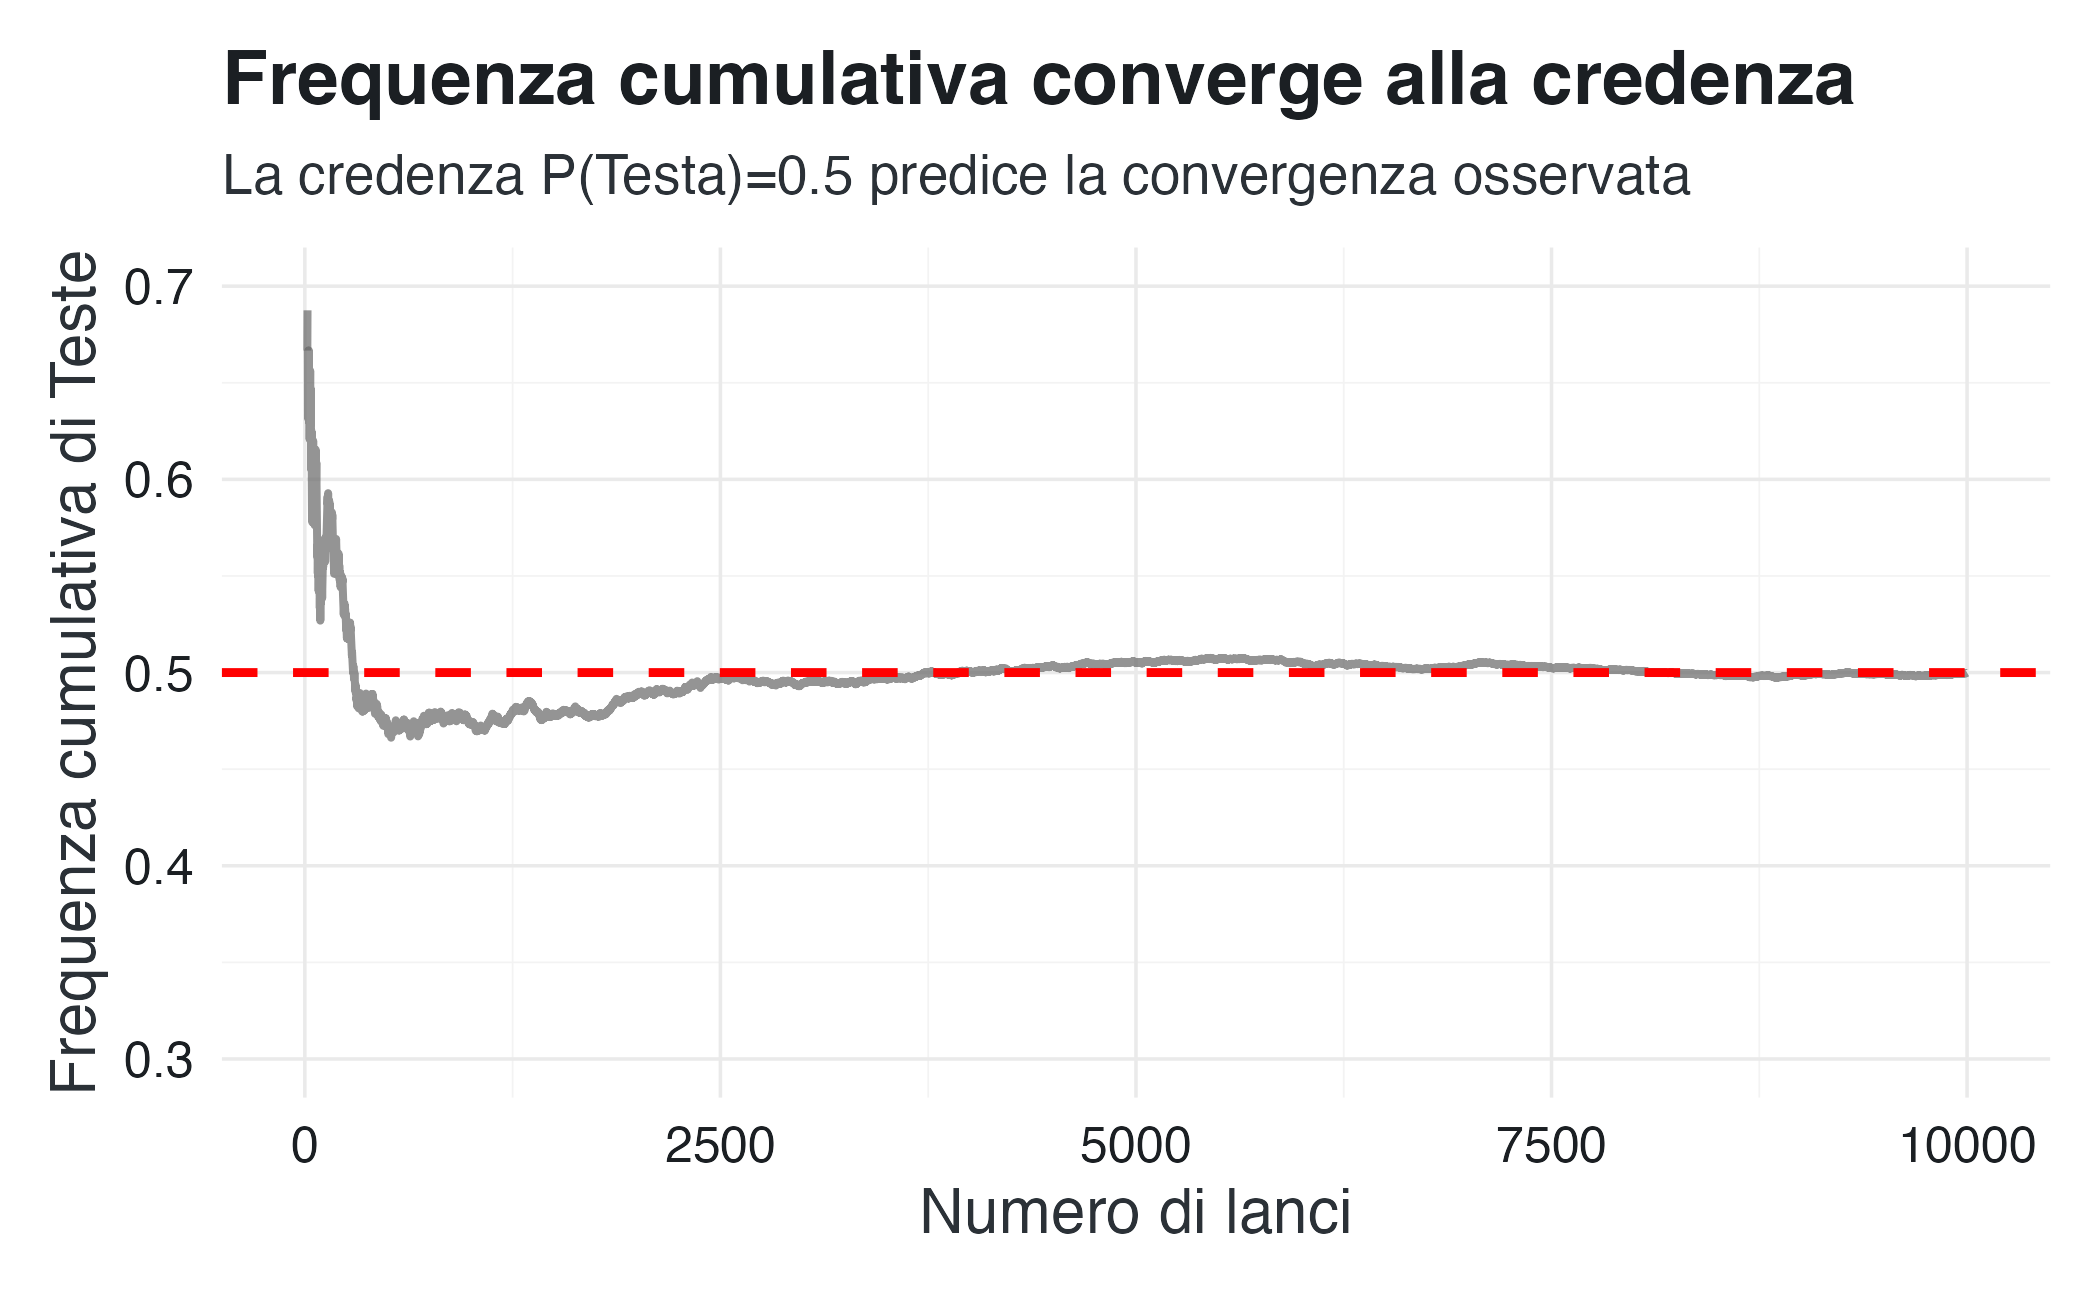
\includegraphics[width=0.85\linewidth,height=\textheight,keepaspectratio]{chapters/probability/01_intro_prob_bayesian_files/figure-pdf/unnamed-chunk-2-1.png}
\end{center}

L'interpretazione bayesiana di questa simulazione evidenzia che
l'assegnazione di \(P(\text{Testa}) = 0.5\) deriva da un principio di
simmetria epistemica, in assenza di informazioni che privilegino un
esito rispetto all'altro. La simulazione verifica la coerenza di questa
credenza con il comportamento empirico atteso. È importante notare che
la probabilità 0.5 non è definita dalla convergenza empirica, ma
rappresenta un'assegnazione a priori che la legge dei grandi numeri
successivamente conferma.

\section{Introduzione all'aggiornamento
bayesiano}\label{introduzione-allaggiornamento-bayesiano}

Un principio cardine dell'epistemologia bayesiana è che un agente
razionale possiede credenze di diversa intensità, soggette ai vincoli di
coerenza imposti dagli assiomi della probabilità. Sia lo stato attuale
di una credenza sia la sua evoluzione all'arrivo di nuove informazioni
possono essere rappresentati mediante distribuzioni di probabilità.

\subsection{Il principio di
condizionamento}\label{il-principio-di-condizionamento}

Il \textbf{principio di condizionamento} specifica come un agente
razionale debba rivedere le proprie credenze quando emergono nuove
evidenze. Esso traduce il concetto di probabilità condizionata in una
regola operativa: la probabilità iniziale (o \emph{a priori}) di
un'ipotesi \(H\) viene trasformata nella sua probabilità finale (o
\emph{a posteriori}) dopo l'osservazione di un dato \(E\) rilevante.

Più che un assioma, si tratta di una \textbf{prescrizione di coerenza
dinamica}: impone che il nuovo grado di fiducia in \(H\) coincida con la
probabilità che gli si attribuiva inizialmente, \emph{dato che} si è
verificato \(E\). L'informazione nuova viene così incorporata in modo
sistematico, evitando aggiustamenti arbitrari e garantendo che la
revisione rimanga ancorata allo stato di conoscenza precedente.

\subsection{Il teorema di Bayes: struttura
concettuale}\label{il-teorema-di-bayes-struttura-concettuale}

Il \textbf{teorema di Bayes} è lo strumento matematico che realizza il
principio di condizionamento, scomponendo la credenza aggiornata in tre
componenti essenziali:

\begin{enumerate}
\def\labelenumi{\arabic{enumi}.}
\tightlist
\item
  \textbf{Probabilità a priori} \(P(H)\): il grado di fiducia iniziale
  nell'ipotesi, prima di osservare i dati.
\item
  \textbf{Verosimiglianza} \(P(E \mid H)\): la plausibilità
  dell'evidenza \(E\) \emph{supponendo vera} l'ipotesi \(H\), ovvero
  quanto il dato osservato sia compatibile con l'ipotesi.
\item
  \textbf{Probabilità marginale dell'evidenza} \(P(E)\): un fattore di
  normalizzazione che assicura la coerenza, pari alla probabilità
  complessiva di osservare \(E\) sotto tutte le ipotesi considerate.
\end{enumerate}

Il teorema mostra come una credenza iniziale, \(P(H)\), venga modulata
dalla forza dell'evidenza, \(P(E \mid H)\), per generare una credenza
finale, \(P(H \mid E)\). È il nucleo matematico dell'apprendimento
dall'esperienza: l'aggiornamento sistematico e coerente delle opinioni
alla luce di nuovi dati.

\subsection{Un esempio anticipatorio: i test
diagnostici}\label{un-esempio-anticipatorio-i-test-diagnostici}

Un esempio paradigmatico di aggiornamento bayesiano è l'interpretazione
di un test diagnostico. Qui l'ipotesi \(H\) è la presenza di una
malattia, mentre l'evidenza \(E\) è un risultato positivo.

La probabilità a priori riflette la prevalenza della malattia nella
popolazione. La verosimiglianza è espressa dalla sensibilità del test
(probabilità di un positivo in un malato) e dal tasso di falsi positivi
(probabilità di un positivo in un sano). Combinando questi elementi, il
teorema restituisce la probabilità a posteriori di malattia dopo un
esito positivo.

L'esempio illustra un principio generale: \textbf{l'evidenza assume
significato solo alla luce delle conoscenze pregresse}. Un test anche
molto accurato può condurre a una probabilità a posteriori
sorprendentemente bassa se la malattia era inizialmente rara. Questa è
la radice della cosiddetta \emph{fallacia del tasso base}: la tendenza,
ben documentata in psicologia cognitiva, a sovrastimare
\(P(\text{malattia} \mid \text{positivo})\) trascurando la prevalenza.
Il teorema di Bayes non è quindi soltanto una regola di calcolo, ma un
correttivo normativo a una delle più robuste distorsioni del
ragionamento umano.

L'esempio verrà ripreso e sviluppato numericamente nei capitoli
successivi, dove mostreremo come la combinazione di \emph{prior} e
verosimiglianza possa produrre esiti controintuitivi ma logicamente
inattaccabili.

\subsection{Sintesi concettuale}\label{sintesi-concettuale}

L'aggiornamento bayesiano può essere rappresentato nella sua essenza
come:

\[
\underbrace{P(H)}_{\text{prior}}
\;\xrightarrow[\text{osservazione dei dati}]{\text{aggiornamento bayesiano}}\;
\underbrace{P(H \mid E)}_{\text{posterior}}.
\]

Questa sintesi visuale coglie il cuore dell'inferenza bayesiana: un
modello formale del ragionamento che integra nuove informazioni con le
conoscenze acquisite, senza né ignorare i dati né cedere a
sopravvalutazioni. Il teorema di Bayes, in questa prospettiva, si rivela
non solo uno strumento matematico, ma una guida razionale per orientarsi
e decidere in condizioni di incertezza.

\section{La probabilità bayesiana nella ricerca
psicologica}\label{la-probabilituxe0-bayesiana-nella-ricerca-psicologica}

La teoria bayesiana della probabilità si rivela particolarmente adatta
allo studio dei fenomeni psicologici, poiché fornisce strumenti
concettuali e metodologici per affrontare in modo esplicito e coerente
l'incertezza che caratterizza sia la ricerca empirica sia la pratica
clinica.

\subsection{Quantificare l'incertezza in ambito clinico e
cognitivo}\label{quantificare-lincertezza-in-ambito-clinico-e-cognitivo}

In ambito diagnostico, il framework bayesiano consente di integrare
sistematicamente fonti informative eterogenee --- anamnesi, osservazione
comportamentale, test psicometrici --- aggiornando le credenze del
clinico a ogni nuova evidenza. Un contributo particolarmente rilevante è
la possibilità di incorporare esplicitamente la prevalenza dei disturbi,
riducendo il rischio di errori dovuti alla negligenza dei tassi di base.

Nello studio dei processi cognitivi, un influente filone di ricerca
propone che molti aspetti del funzionamento mentale possano essere
descritti come approssimazioni di un ragionamento bayesiano ideale
(Griffiths et al., 2024). La percezione, ad esempio, può essere
modellata come integrazione tra aspettative pregresse e informazioni
sensoriali --- spiegando fenomeni come le illusioni percettive ---
mentre l'apprendimento e molti bias cognitivi trovano una loro
interpretazione naturale come aggiornamenti imperfetti o scostamenti
dall'ottimalità bayesiana.

Sul piano metodologico, l'inferenza bayesiana offre vantaggi concreti
nell'analisi dei dati psicologici: incorporazione formalizzata delle
conoscenze pregresse, quantificazione diretta dell'evidenza a favore di
ipotesi specifiche, gestione naturale di campioni ridotti e propagazione
coerente dell'incertezza attraverso modelli statistici complessi.

In ambito terapeutico, infine, l'approccio consente di aggiornare
sequenzialmente le stime di efficacia degli interventi, adattando i
protocolli alle risposte del singolo paziente e bilanciando probabilità
ed esiti attesi nelle scelte cliniche.

\subsection{Un quadro epistemologico
coerente}\label{un-quadro-epistemologico-coerente}

Diversamente dal frequentismo --- che definisce la probabilità come
frequenza relativa in una sequenza ideale infinita di prove ripetute e
considera i parametri come quantità fisse ma ignote --- l'approccio
bayesiano interpreta la probabilità come grado di credenza razionale,
tratta i parametri come variabili aleatorie che rappresentano
l'incertezza dell'osservatore e consente di formulare affermazioni del
tipo: ``La probabilità che l'effetto del trattamento sia positivo è pari
a 0.85''.

Ne deriva un'interpretazione diretta degli intervalli di stima: un
intervallo di credibilità al 95\% esprime, dati i risultati osservati e
il modello adottato, che esiste una probabilità del 95\% che il
parametro cada al suo interno. Un vantaggio operativo non trascurabile
per chi deve prendere decisioni cliniche o di policy.

L'approccio bayesiano non sostituisce l'inferenza frequentista, ma la
integra in un quadro epistemologico più ampio, in cui la soggettività
delle credenze iniziali viene resa esplicita e vincolata dalla coerenza
formale, e l'evidenza empirica modula le opinioni in modo trasparente e
verificabile.

\section*{Riflessioni conclusive}\label{riflessioni-conclusive}

\markright{Riflessioni conclusive}

Abbiamo iniziato questo capitolo con una domanda: perché la probabilità
bayesiana in psicologia? La risposta che abbiamo fornito è che la
probabilità, intesa come grado di credenza razionale, offre un
linguaggio unitario per quantificare l'incertezza, sia quella che deriva
dai limiti della nostra conoscenza, sia quella che sembra inerente ai
fenomeni stessi. Questa prospettiva, che affonda le proprie radici in
Bayes, Laplace e de Finetti, non è un tecnicismo matematico, ma una
\textbf{lente interpretativa} attraverso cui leggere il ragionamento
umano in condizioni di incertezza.

Abbiamo visto che gli assiomi della probabilità non sono mere
convenzioni formali, ma \textbf{principi di coerenza} che vincolano le
nostre credenze: violarli significa esporsi a contraddizioni interne e a
decisioni sistematicamente svantaggiose, come dimostrato dall'argomento
della scommessa olandese. Abbiamo anche compreso che, nel quadro
bayesiano, l'incertezza non è più una proprietà del mondo che emerge
solo in lunghe sequenze di prove, ma una misura della nostra conoscenza
imperfetta, applicabile anche a eventi singoli e non ripetibili, come la
prognosi di un paziente o l'esito di una decisione clinica.

Questo cambiamento di prospettiva ha implicazioni concrete per la
ricerca psicologica. L'approccio bayesiano rende esplicite le assunzioni
iniziali attraverso la scelta del prior, formalizza l'apprendimento dai
dati con il teorema di Bayes e fornisce strumenti per gestire la
complessità dei modelli statistici senza rinunciare alla trasparenza.
Non elimina l'incertezza --- che nella psicologia è una
\textbf{condizione strutturale}, non un'eccezione --- ma fornisce un
linguaggio per quantificarla, comunicarla e integrarla nelle decisioni.

Nei prossimi capitoli trasformeremo queste idee in strumenti operativi.
Scopriremo come costruire un modello bayesiano, come scegliere i
\emph{prior} e come interpretare i risultati. Inoltre, vedremo che
concetti come l'equiprobabilità, spesso considerati oggettivi,
riflettono in realtà simmetrie nel nostro stato informativo. L'obiettivo
non è eliminare l'incertezza --- compito impossibile, nella psicologia
--- ma imparare a ragionare con essa, trasformandola da ostacolo in
risorsa.

\section*{Punti chiave da ricordare}\label{punti-chiave-da-ricordare}
\addcontentsline{toc}{section}{Punti chiave da ricordare}

\markright{Punti chiave da ricordare}

\begin{tcolorbox}[enhanced jigsaw, arc=.35mm, bottomrule=.15mm, bottomtitle=1mm, breakable, colback=white, colbacktitle=quarto-callout-important-color!10!white, colframe=quarto-callout-important-color-frame, coltitle=black, left=2mm, leftrule=.75mm, opacityback=0, opacitybacktitle=0.6, rightrule=.15mm, title=\textcolor{quarto-callout-important-color}{\faExclamation}\hspace{0.5em}{Importante}, titlerule=0mm, toprule=.15mm, toptitle=1mm]

\textbf{Concetti essenziali di questo capitolo:}

\begin{enumerate}
\def\labelenumi{\arabic{enumi}.}
\tightlist
\item
  \textbf{Interpretazione soggettivista della probabilità}

  \begin{itemize}
  \tightlist
  \item
    La probabilità misura il grado di credenza razionale di un agente
    riguardo a un evento incerto
  \item
    È personale ma non arbitraria: deve rispettare regole di coerenza
  \end{itemize}
\item
  \textbf{Differenza con l'approccio frequentista}

  \begin{itemize}
  \tightlist
  \item
    Frequentista: probabilità come limite di frequenze relative
    (ripetibilità)
  \item
    Bayesiano: probabilità come quantificazione dell'incertezza
    epistemica
  \end{itemize}
\item
  \textbf{Applicabilità universale}

  \begin{itemize}
  \tightlist
  \item
    L'approccio bayesiano si applica a eventi non ripetibili (es.
    probabilità che piova domani, che un'ipotesi scientifica sia vera)
  \end{itemize}
\end{enumerate}

\textbf{Per il prossimo capitolo:}

Nel Capitolo~\ref{sec-prob-axioms-coherence} vedremo come le regole di
coerenza delle credenze si formalizzano negli assiomi della probabilità,
garantendo che i nostri gradi di credenza siano internamente
consistenti.

\end{tcolorbox}

\begin{tcolorbox}[enhanced jigsaw, arc=.35mm, bottomrule=.15mm, bottomtitle=1mm, breakable, colback=white, colbacktitle=quarto-callout-note-color!10!white, colframe=quarto-callout-note-color-frame, coltitle=black, left=2mm, leftrule=.75mm, opacityback=0, opacitybacktitle=0.6, rightrule=.15mm, title=\textcolor{quarto-callout-note-color}{\faInfo}\hspace{0.5em}{Informazioni sull'ambiente di sviluppo}, titlerule=0mm, toprule=.15mm, toptitle=1mm]

\begin{Shaded}
\begin{Highlighting}[]
\FunctionTok{sessionInfo}\NormalTok{()}
\CommentTok{\#\textgreater{} R version 4.6.1 (2026{-}06{-}24)}
\CommentTok{\#\textgreater{} Platform: aarch64{-}apple{-}darwin23}
\CommentTok{\#\textgreater{} Running under: macOS Tahoe 26.5.2}
\CommentTok{\#\textgreater{} }
\CommentTok{\#\textgreater{} Matrix products: default}
\CommentTok{\#\textgreater{} BLAS:   /Library/Frameworks/R.framework/Versions/4.6/Resources/lib/libRblas.0.dylib }
\CommentTok{\#\textgreater{} LAPACK: /Library/Frameworks/R.framework/Versions/4.6/Resources/lib/libRlapack.dylib;  LAPACK version 3.12.1}
\CommentTok{\#\textgreater{} }
\CommentTok{\#\textgreater{} locale:}
\CommentTok{\#\textgreater{} [1] C.UTF{-}8/UTF{-}8/C.UTF{-}8/C/C.UTF{-}8/C.UTF{-}8}
\CommentTok{\#\textgreater{} }
\CommentTok{\#\textgreater{} time zone: Europe/Rome}
\CommentTok{\#\textgreater{} tzcode source: internal}
\CommentTok{\#\textgreater{} }
\CommentTok{\#\textgreater{} attached base packages:}
\CommentTok{\#\textgreater{} [1] stats     graphics  grDevices utils     datasets  methods   base     }
\CommentTok{\#\textgreater{} }
\CommentTok{\#\textgreater{} other attached packages:}
\CommentTok{\#\textgreater{}  [1] ragg\_1.5.2            tinytable\_0.17.0      withr\_3.0.3          }
\CommentTok{\#\textgreater{}  [4] systemfonts\_1.3.2     patchwork\_1.3.2       ggdist\_3.3.3         }
\CommentTok{\#\textgreater{}  [7] tidybayes\_3.0.7       bayesplot\_1.15.0      ggplot2\_4.0.3        }
\CommentTok{\#\textgreater{} [10] reliabilitydiag\_0.2.1 priorsense\_1.2.0      posterior\_1.7.0      }
\CommentTok{\#\textgreater{} [13] loo\_2.10.0            rstan\_2.32.7          StanHeaders\_2.32.10  }
\CommentTok{\#\textgreater{} [16] brms\_2.23.0           Rcpp\_1.1.2            sessioninfo\_1.2.4    }
\CommentTok{\#\textgreater{} [19] conflicted\_1.2.0      janitor\_2.2.1         matrixStats\_1.5.0    }
\CommentTok{\#\textgreater{} [22] modelr\_0.1.11         tibble\_3.3.1          dplyr\_1.2.1          }
\CommentTok{\#\textgreater{} [25] tidyr\_1.3.2           rio\_1.3.0             here\_1.0.2           }
\CommentTok{\#\textgreater{} }
\CommentTok{\#\textgreater{} loaded via a namespace (and not attached):}
\CommentTok{\#\textgreater{}  [1] svUnit\_1.0.8          tidyselect\_1.2.1      farver\_2.1.2         }
\CommentTok{\#\textgreater{}  [4] S7\_0.2.2              fastmap\_1.2.0         tensorA\_0.36.2.1     }
\CommentTok{\#\textgreater{}  [7] digest\_0.6.39         timechange\_0.4.0      estimability\_2.0.0   }
\CommentTok{\#\textgreater{} [10] lifecycle\_1.0.5       magrittr\_2.0.5        compiler\_4.6.1       }
\CommentTok{\#\textgreater{} [13] rlang\_1.3.0           tools\_4.6.1           yaml\_2.3.12          }
\CommentTok{\#\textgreater{} [16] knitr\_1.51            labeling\_0.4.3        bridgesampling\_1.2{-}1 }
\CommentTok{\#\textgreater{} [19] pkgbuild\_1.4.8        curl\_7.1.0            RColorBrewer\_1.1{-}3   }
\CommentTok{\#\textgreater{} [22] abind\_1.4{-}8           purrr\_1.2.2           grid\_4.6.1           }
\CommentTok{\#\textgreater{} [25] stats4\_4.6.1          xtable\_1.8{-}8          inline\_0.3.21        }
\CommentTok{\#\textgreater{} [28] emmeans\_2.0.3         scales\_1.4.0          cli\_3.6.6            }
\CommentTok{\#\textgreater{} [31] mvtnorm\_1.4{-}1         rmarkdown\_2.31        generics\_0.1.4       }
\CommentTok{\#\textgreater{} [34] otel\_0.2.0            RcppParallel\_5.1.11{-}2 cachem\_1.1.0         }
\CommentTok{\#\textgreater{} [37] stringr\_1.6.0         parallel\_4.6.1        vctrs\_0.7.3          }
\CommentTok{\#\textgreater{} [40] V8\_8.2.0              Matrix\_1.7{-}5          jsonlite\_2.0.0       }
\CommentTok{\#\textgreater{} [43] arrayhelpers\_1.1{-}1    glue\_1.8.1            codetools\_0.2{-}20     }
\CommentTok{\#\textgreater{} [46] distributional\_0.8.1  lubridate\_1.9.5       stringi\_1.8.7        }
\CommentTok{\#\textgreater{} [49] gtable\_0.3.6          QuickJSR\_1.10.0       pillar\_1.11.1        }
\CommentTok{\#\textgreater{} [52] htmltools\_0.5.9       Brobdingnag\_1.2{-}9     R6\_2.6.1             }
\CommentTok{\#\textgreater{} [55] textshaping\_1.0.5     rprojroot\_2.1.1       evaluate\_1.0.5       }
\CommentTok{\#\textgreater{} [58] lattice\_0.22{-}9        backports\_1.5.1       memoise\_2.0.1        }
\CommentTok{\#\textgreater{} [61] broom\_1.0.13          snakecase\_0.11.1      rstantools\_2.6.0     }
\CommentTok{\#\textgreater{} [64] coda\_0.19{-}4.1         gridExtra\_2.3.1       nlme\_3.1{-}169         }
\CommentTok{\#\textgreater{} [67] checkmate\_2.3.4       xfun\_0.60             pkgconfig\_2.0.3}
\end{Highlighting}
\end{Shaded}

\end{tcolorbox}

\section*{Bibliografia}\label{bibliografia}

\markright{Bibliografia}

\chapter{Assiomi e coerenza delle
credenze}\label{sec-prob-axioms-coherence}

\section*{Introduzione}\label{introduzione-1}

\markright{Introduzione}

Nel capitolo precedente abbiamo visto che, nell'interpretazione
bayesiana, la probabilità non descrive frequenze oggettive, ma
\textbf{gradi di credenza razionale}. Questa idea, apparentemente
semplice, solleva immediatamente una domanda cruciale: cosa significa,
esattamente, che una credenza sia ``razionale''?

Non basta avere opinioni: tutti ne abbiamo. Non basta nemmeno avere
opinioni informate o ragionevoli. Il punto è più sottile e profondo: le
nostre credenze devono essere \textbf{internamente coerenti} tra loro.
Se, per esempio, credo che pioverà con probabilità 0.7 e che non pioverà
con probabilità 0.5, sto commettendo un errore logico, a prescindere da
quanto siano informate le mie valutazioni meteorologiche. La somma delle
mie credenze su eventi mutuamente esclusivi ed esaustivi deve essere 1,
non per una convenzione arbitraria, ma perché altrimenti il mio sistema
di credenze si contraddice.

Questo capitolo sviluppa il quadro matematico che rende espliciti e
controllabili questi vincoli di coerenza. Ma attenzione: non si tratta
di aggiungere un livello puramente formale alla discussione. La
matematica che introdurremo non è un semplice ornamento tecnico, ma il
\emph{linguaggio} attraverso cui possiamo esprimere con precisione il
significato di un ragionamento coerente in condizioni di incertezza.

\subsection*{Perché questo è importante per la
psicologia}\label{perchuxe9-questo-uxe8-importante-per-la-psicologia}

Per gli psicologi, questi assiomi definiscono lo standard normativo
contro cui valutare il ragionamento umano in condizioni di incertezza,
un tema centrale nella ricerca sui bias cognitivi a partire da Kahneman
e Tversky. Inoltre, quando costruiamo modelli statistici, la coerenza
probabilistica non è un optional: un modello incoerente è logicamente
impossibile, come un triangolo con quattro lati. Comprendere questi
vincoli ci rende ricercatori più consapevoli e clinici più competenti.

\begin{tcolorbox}[enhanced jigsaw, arc=.35mm, bottomrule=.15mm, bottomtitle=1mm, breakable, colback=white, colbacktitle=quarto-callout-tip-color!10!white, colframe=quarto-callout-tip-color-frame, coltitle=black, left=2mm, leftrule=.75mm, opacityback=0, opacitybacktitle=0.6, rightrule=.15mm, title=\textcolor{quarto-callout-tip-color}{\faLightbulb}\hspace{0.5em}{Prerequisiti}, titlerule=0mm, toprule=.15mm, toptitle=1mm]

Per seguire questo capitolo è necessario aver letto:

\begin{itemize}
\tightlist
\item
  Capitolo~\ref{sec-prob-interpretation}
\end{itemize}

Conoscenze matematiche richieste:

\begin{itemize}
\tightlist
\item
  Appendice~\ref{sec-apx-sums} - per comprendere le proprietà additive
\item
  Appendice~\ref{sec-apx-sets} - per operazioni su eventi (unione,
  intersezione, complemento)
\end{itemize}

\end{tcolorbox}

\subsection*{Panoramica del capitolo}\label{panoramica-del-capitolo}

Il percorso che seguiremo è questo:

\begin{enumerate}
\def\labelenumi{\arabic{enumi}.}
\item
  Reinterpreteremo lo \textbf{spazio campionario} non come l'insieme
  degli esiti fisicamente possibili, ma come l'insieme delle possibilità
  che \emph{noi} consideriamo date le nostre informazioni.
\item
  Vedremo come gli \textbf{eventi} diventino \emph{proposizioni} sul
  mondo a cui assegniamo gradi di credenza.
\item
  Introdurremo gli \textbf{assiomi di Kolmogorov} non come regole
  arbitrarie, ma come vincoli \emph{necessari} per evitare
  auto-contraddizioni.
\item
  Impareremo a \textbf{diagnosticare incoerenze} nelle assegnazioni
  probabilistiche.
\item
  Costruiremo \textbf{tabelle di probabilità congiunta}, lo strumento
  operativo fondamentale per rappresentare sistemi di credenze
  complessi.
\item
  Mostreremo come tutte le probabilità di interesse (marginali,
  condizionate) \textbf{derivino} dalla distribuzione congiunta.
\end{enumerate}

\begin{tcolorbox}[enhanced jigsaw, arc=.35mm, bottomrule=.15mm, bottomtitle=1mm, breakable, colback=white, colbacktitle=quarto-callout-caution-color!10!white, colframe=quarto-callout-caution-color-frame, coltitle=black, left=2mm, leftrule=.75mm, opacityback=0, opacitybacktitle=0.6, rightrule=.15mm, title=\textcolor{quarto-callout-caution-color}{\faFire}\hspace{0.5em}{Preparazione del Notebook}, titlerule=0mm, toprule=.15mm, toptitle=1mm]

\begin{Shaded}
\begin{Highlighting}[]
\NormalTok{here}\SpecialCharTok{::}\FunctionTok{here}\NormalTok{(}\StringTok{"code"}\NormalTok{, }\StringTok{"\_common.R"}\NormalTok{) }\SpecialCharTok{|\textgreater{}} 
  \FunctionTok{source}\NormalTok{()}

\CommentTok{\# Load packages}
\ControlFlowTok{if}\NormalTok{ (}\SpecialCharTok{!}\FunctionTok{requireNamespace}\NormalTok{(}\StringTok{"pacman"}\NormalTok{)) }\FunctionTok{install.packages}\NormalTok{(}\StringTok{"pacman"}\NormalTok{)}
\NormalTok{pacman}\SpecialCharTok{::}\FunctionTok{p\_load}\NormalTok{(viridis)}
\CommentTok{\# Riapplica il tema per sicurezza}
\FunctionTok{apply\_visual\_theme}\NormalTok{()}
\end{Highlighting}
\end{Shaded}

\end{tcolorbox}

\section{Spazio campionario come possibilità
epistemiche}\label{spazio-campionario-come-possibilituxe0-epistemiche}

Prima di addentrarci nelle definizioni formali, fermiamoci a riflettere
su cosa stiamo cercando di catturare.

Quando uno psicologo clinico valuta un paziente, non sta osservando un
``esperimento casuale'' nel senso fisico del termine. Non c'è un dado
che rotola, né una moneta che viene lanciata. Eppure, il clinico si
trova in una condizione di \emph{incertezza genuina}: sulla base delle
informazioni raccolte (anamnesi, colloquio, test), deve formarsi
un'opinione su quale sia la condizione del paziente tra diverse
possibilità.

Questa situazione, ovvero avere informazioni incomplete e dover
ragionare su possibilità alternative, è esattamente ciò che la teoria
della probabilità, nell'interpretazione bayesiana, è progettata per
gestire. Il primo passo è definire le possibilità che stiamo prendendo
in considerazione.

\begin{definition}[Spazio
campionario]\protect\hypertarget{def-sample-space-bayesian}{}\label{def-sample-space-bayesian}

Lo \emph{spazio campionario} \(\Omega\) rappresenta l'insieme delle
\emph{possibilità epistemiche} compatibili con lo stato informativo
corrente. Esso non descrive necessariamente tutto ciò che può accadere
fisicamente, ma piuttosto ciò che, dati i limiti della nostra
conoscenza, consideriamo logicamente possibile.

\end{definition}

\subsection{Un cambio di prospettiva
fondamentale}\label{un-cambio-di-prospettiva-fondamentale}

Questa definizione merita attenzione. Nella visione frequentista
tradizionale, lo spazio campionario è qualcosa di ``oggettivo'':
l'insieme di tutti gli esiti che un esperimento può produrre,
indipendentemente da chi lo osserva. Nell'approccio bayesiano, invece,
lo spazio campionario diventa \emph{epistemico}: dipende da ciò che
\emph{noi} sappiamo e dalle distinzioni che \emph{noi} riteniamo
rilevanti.

Questo cambiamento non è un dettaglio tecnico, ma un cambio di
prospettiva filosofica con conseguenze pratiche profonde. Ciò significa
che:

\begin{itemize}
\item
  \textbf{ricercatori diversi possono legittimamente usare spazi
  campionari diversi} per lo stesso fenomeno, se hanno informazioni
  diverse o interessi diversi;
\item
  \textbf{lo spazio campionario può cambiare} quando si acquisiscono
  nuove informazioni. Prima di un test diagnostico, consideriamo come
  possibili sia il risultato ``positivo'' che quello ``negativo''; dopo
  aver osservato il risultato, lo spazio delle possibilità rilevanti si
  restringe.
\item
  \textbf{la scelta dello spazio campionario è una decisione di
  modellazione}, non una scoperta empirica; richiede un giudizio su
  quale livello di dettaglio sia appropriato per il problema in esame.
\end{itemize}

\subsection{Caratteristiche dello spazio campionario
epistemico}\label{caratteristiche-dello-spazio-campionario-epistemico}

La composizione dello spazio campionario riflette dunque la natura
informazionale e soggettiva della probabilità bayesiana. Non esiste
``lo'' spazio campionario corretto in senso assoluto, ma esiste quello
appropriato, date le nostre informazioni e i nostri obiettivi.

\begin{tcolorbox}[enhanced jigsaw, arc=.35mm, bottomrule=.15mm, bottomtitle=1mm, breakable, colback=white, colbacktitle=quarto-callout-note-color!10!white, colframe=quarto-callout-note-color-frame, coltitle=black, left=2mm, leftrule=.75mm, opacityback=0, opacitybacktitle=0.6, rightrule=.15mm, title=\textcolor{quarto-callout-note-color}{\faInfo}\hspace{0.5em}{Esempio psicologico: livelli di granularità nella valutazione clinica}, titlerule=0mm, toprule=.15mm, toptitle=1mm]

Consideriamo la valutazione di un paziente per una possibile
depressione. Lo spazio campionario può essere definito a diversi
livelli, a seconda delle informazioni disponibili e degli obiettivi
clinici:

\textbf{Livello 1 (binario):}

\[\Omega_1 = \{\text{Depresso}, \text{Non depresso}\}.\]

Questo è il livello appropriato per una decisione sì/no: il paziente
necessita di trattamento per depressione?

\textbf{Livello 2 (severità):}

\[\Omega_2 = \{\text{Nessuna}, \text{Lieve}, \text{Moderata}, \text{Severa}\}.\]

Qui distinguiamo gradi di severità, che sono importanti quando dobbiamo
decidere \emph{quale tipo} di trattamento proporre.

\textbf{Livello 3 (combinazioni diagnostiche):}

\[\Omega_3 = \{\text{Depressione}, \text{Ansia}, \text{Comorbidità}, \text{Nessuna}\}.\]

Questo livello considera la possibilità di diagnosi multiple o
alternative.

Nessuno di questi spazi campionari è ``più corretto'' degli altri in
senso assoluto. La scelta dipende da:

\begin{itemize}
\tightlist
\item
  le \textbf{informazioni disponibili} (uno screening rapido vs.~una
  valutazione approfondita);
\item
  l'\textbf{obiettivo dell'analisi} (screening di popolazione
  vs.~diagnosi differenziale);
\item
  le \textbf{decisioni da prendere} (inviare a uno specialista o
  pianificare un trattamento specifico).
\end{itemize}

La consapevolezza che lo spazio campionario è una \emph{scelta} di
modellazione e non un dato di fatto è il primo passo verso un uso maturo
della probabilità.

\end{tcolorbox}

\section{Eventi come proposizioni sul
mondo}\label{eventi-come-proposizioni-sul-mondo}

Una volta definito lo spazio delle possibilità, il passo successivo è
considerare le \emph{affermazioni} su queste possibilità. Qui avviene
un'altra importante traduzione concettuale.

Nella teoria degli insiemi, un ``evento'' è semplicemente un
sottoinsieme dello spazio campionario. Tuttavia, nell'interpretazione
epistemica, un evento acquista un significato più ricco: diventa una
\emph{proposizione}, un'affermazione sul mondo che può essere vera o
falsa.

\begin{definition}[Evento]\protect\hypertarget{def-event-bayesian}{}\label{def-event-bayesian}

Un \emph{evento} \(A \subseteq \Omega\) è una \emph{proposizione} alla
quale possiamo assegnare un grado di credenza \(P(A)\), condizionato
allo stato informativo corrente.

\end{definition}

\subsection{La logica delle proposizioni
incerte}\label{la-logica-delle-proposizioni-incerte}

Questa interpretazione collega la teoria della probabilità alla logica
proposizionale. Le operazioni insiemistiche diventano operazioni
logiche:

\begin{itemize}
\tightlist
\item
  L'\textbf{unione} \(A \cup B\) corrisponde alla disgiunzione logica:
  ``\(A\) \emph{oppure} \(B\) è vera'' (o entrambe).
\item
  L'\textbf{intersezione} \(A \cap B\) corrisponde alla congiunzione
  logica: ``\(A\) \emph{e} \(B\) sono entrambe vere''.
\item
  Il \textbf{complemento} \(A^c\) corrisponde alla negazione: ``\(A\) è
  falsa''.
\end{itemize}

Questa corrispondenza non è casuale. La teoria della probabilità può
essere considerata come un'\emph{estensione} della logica classica al
caso dell'incertezza. Mentre la logica classica assegna solo valori
``vero'' (1) o ``falso'' (0) alle proposizioni, la probabilità assegna
valori intermedi che rappresentano \emph{gradi} di credenza.

L'\textbf{insieme vuoto} \(\varnothing\) corrisponde a una proposizione
logicamente contraddittoria, qualcosa che non può essere vero in nessuna
delle possibilità che prendiamo in considerazione. Al contrario, lo
\textbf{spazio campionario} \(\Omega\) corrisponde a una tautologia,
qualcosa che è necessariamente vero, dato che una delle possibilità deve
realizzarsi.

\begin{tcolorbox}[enhanced jigsaw, arc=.35mm, bottomrule=.15mm, bottomtitle=1mm, breakable, colback=white, colbacktitle=quarto-callout-note-color!10!white, colframe=quarto-callout-note-color-frame, coltitle=black, left=2mm, leftrule=.75mm, opacityback=0, opacitybacktitle=0.6, rightrule=.15mm, title=\textcolor{quarto-callout-note-color}{\faInfo}\hspace{0.5em}{Esempio: Eventi in un test psicometrico}, titlerule=0mm, toprule=.15mm, toptitle=1mm]

La \emph{Satisfaction with Life Scale} (SWLS) produce punteggi compresi
tra 5 e 35. Definiamo:

\begin{itemize}
\tightlist
\item
  \(\Omega = \{5, 6, 7, \ldots, 35\}\) (punteggi possibili);
\item
  \(A =\) ``Punteggio ≥ 25'' (alta soddisfazione)
  \(= \{25, 26, \ldots, 35\}\);
\item
  \(B =\) ``Punteggio ≤ 15'' (bassa soddisfazione)
  \(= \{5, 6, \ldots, 15\}\);
\item
  \(C =\) ``Punteggio tra 16 e 24'' (soddisfazione moderata)
  \(= \{16, 17, \ldots, 24\}\).
\end{itemize}

Alcune operazioni sugli eventi e il loro significato:

\begin{itemize}
\tightlist
\item
  \(A \cup B\): ``La persona ha soddisfazione alta \emph{oppure} bassa''
  (estremi).
\item
  \(A \cap B = \varnothing\): ``Alta \emph{e} bassa soddisfazione
  insieme''---impossibile per definizione.
\item
  \(A^c = B \cup C\): ``Non alta soddisfazione'' = ``soddisfazione bassa
  o moderata''.
\item
  \(A \cup B \cup C = \Omega\): le tre categorie esauriscono tutte le
  possibilità.
\end{itemize}

Quando assegniamo \(P(A) = 0.30\), stiamo dicendo: ``Dato ciò che so
della popolazione di riferimento e del contesto di valutazione, ritengo
plausibile che un individuo selezionato presenti un'alta soddisfazione
di vita con una probabilità del 30\%''

Questa è un'affermazione epistemica, non una frequenza oggettiva. Due
ricercatori con informazioni diverse potrebbero legittimamente assegnare
valori diversi.

\end{tcolorbox}

\section{Gli assiomi di Kolmogorov come vincoli di
coerenza}\label{gli-assiomi-di-kolmogorov-come-vincoli-di-coerenza}

Arriviamo ora al cuore concettuale del capitolo. Abbiamo visto che le
probabilità sono gradi di credenza su proposizioni. Ma quali valori
possiamo assegnare? Siamo liberi di scegliere qualsiasi numero ci
piaccia?

La risposta è no, e capire \emph{perché} è fondamentale.

\subsection{Il problema della
coerenza}\label{il-problema-della-coerenza}

Immaginiamo un clinico che, valutando un paziente, assegna le seguenti
probabilità a tre diagnosi mutualmente esclusive:

\begin{itemize}
\tightlist
\item
  \(P(\text{Schizofrenia}) = 0.6\)
\item
  \(P(\text{Disturbo Bipolare}) = 0.5\)
\item
  \(P(\text{Nessun disturbo psicotico}) = 0.2\)
\end{itemize}

La somma è 1.3. Cosa significa? Significa che il clinico sta assegnando
più certezza di quanta ne abbia a disposizione. È come se il clinico
dicesse: ``Sono sicuro al 130\% che una di queste tre cose sia vera'',
il che non ha senso.

Questo non è un errore di valutazione clinica (il clinico potrebbe avere
ottime ragioni per ciascuna stima individuale). Si tratta di un errore
\emph{logico}: le credenze sono in contraddizione tra loro. Come abbiamo
visto nel capitolo precedente, un sistema di credenze incoerente espone
a perdite certe (l'argomento della scommessa olandese).

Gli assiomi che introduciamo ora sono precisamente i vincoli che
\emph{impediscono} questo tipo di auto-contraddizioni.

\begin{definition}[Funzione di
probabilità]\protect\hypertarget{def-probability-measure}{}\label{def-probability-measure}

Una \emph{funzione di probabilità} è una funzione \[
P: \mathcal{F} \to [0,1],
\] che assegna a ogni evento \(A\) appartenente a una famiglia di eventi
\(\mathcal{F}\) il numero \(P(A)\), interpretabile come il grado di
credenza nell'affermazione \(A\), dato lo stato informativo corrente.

Per essere \emph{coerente}, la funzione \(P\) deve soddisfare i seguenti
\textbf{assiomi di coerenza}:

\begin{enumerate}
\def\labelenumi{\arabic{enumi}.}
\item
  \textbf{Non negatività}\\
  \[P(A) \geq 0 \quad \text{per ogni evento } A.\]
\item
  \textbf{Normalizzazione}\\
  \[P(\Omega) = 1.\]
\item
  \textbf{Additività}\\
  Se \(A\) e \(B\) sono eventi mutuamente esclusivi
  (\(A \cap B = \varnothing\)), allora \[P(A \cup B) = P(A) + P(B).\]

  Per spazi campionari infiniti, questo principio si estende a
  successioni numerabili di eventi: se \(A_1, A_2, \ldots\) sono a due a
  due disgiunti, allora
  \[P\!\left(\bigcup_{i=1}^{\infty} A_i\right) = \sum_{i=1}^{\infty} P(A_i).\]
  Nella pratica psicologica, tuttavia, lavoreremo quasi sempre con spazi
  finiti, per cui la versione finita è quella che utilizzeremo più
  spesso.
\end{enumerate}

\end{definition}

\subsection{Perché questi assiomi e non
altri?}\label{perchuxe9-questi-assiomi-e-non-altri}

Una domanda legittima è: perché proprio questi tre (o quattro) vincoli?
La risposta profonda a questa domanda viene dalla teoria della decisione
e dall'argomento della scommessa olandese, che abbiamo trattato nel
capitolo precedente. Tuttavia, è possibile fornire un'interpretazione
intuitiva di ciascun assioma.

\textbf{La non negatività} riflette un fatto semplice: non esiste un
grado di credenza ``meno che impossibile''. Zero significa ``sono certo
che non accadrà''; non c'è nulla al di sotto dello zero. Se qualcuno vi
dicesse: ``Credo che pioverà con probabilità -0.3'', non sapreste
nemmeno cosa intende.

\textbf{La normalizzazione} esprime la convinzione che \emph{qualcosa}
debba accadere. Per costruzione, lo spazio campionario contiene tutte le
possibilità che prendiamo in considerazione. Una di queste deve
realizzarsi. Assegnare \(P(\Omega) < 1\) significherebbe ammettere la
possibilità che nessuna delle alternative si verifichi, ma in tal caso
avremmo dimenticato qualche alternativa nel nostro spazio campionario.

\textbf{L'additività} è forse il vincolo più importante, e merita una
riflessione più approfondita. Dice che, se \(A\) e \(B\) non possono
verificarsi insieme, allora la mia credenza che ``si verifichi \(A\)
oppure \(B\)'' deve essere esattamente la somma delle mie credenze
separate in \(A\) e in \(B\).

Perché? Qualsiasi altra assegnazione sarebbe incoerente. Se assegnassi
\(P(A \cup B) < P(A) + P(B)\), direi che credo ``meno'' nella
disgiunzione rispetto alle due opzioni prese separatamente, ma la
disgiunzione include entrambe le opzioni! Viceversa, se assegnassi
\(P(A \cup B) > P(A) + P(B)\), starei ``contando due volte'' qualcosa.

L'\textbf{additività numerabile} estende questo ragionamento a sequenze
infinite di eventi, necessarie per trattare variabili continue, ma il
principio è lo stesso.

\begin{tcolorbox}[enhanced jigsaw, arc=.35mm, bottomrule=.15mm, bottomtitle=1mm, breakable, colback=white, colbacktitle=quarto-callout-note-color!10!white, colframe=quarto-callout-note-color-frame, coltitle=black, left=2mm, leftrule=.75mm, opacityback=0, opacitybacktitle=0.6, rightrule=.15mm, title=\textcolor{quarto-callout-note-color}{\faInfo}\hspace{0.5em}{Un'analogia utile: le aree}, titlerule=0mm, toprule=.15mm, toptitle=1mm]

Le proprietà della probabilità sono analoghe a quelle delle aree. Se due
regioni non si sovrappongono, la loro area totale è la somma delle due
aree. Se le regioni si sovrappongono, devo sottrarre l'area di
sovrapposizione per evitare di contarla due volte. L'area totale
disponibile (normalizzata a 1) non può essere superata. Nessuna regione
ha un'area negativa.

Questa analogia non è casuale: matematicamente, la probabilità è una
``misura'' e le misure generalizzano il concetto di area/volume.
Tuttavia, l'interpretazione è diversa: non stiamo misurando estensioni
spaziali, ma gradi di credenza.

\end{tcolorbox}

\subsection{Conseguenze immediate degli
assiomi}\label{conseguenze-immediate-degli-assiomi}

Una volta accettati questi vincoli fondamentali, molte altre proprietà
ne derivano come conseguenze logiche necessarie. Non si tratta di regole
aggiuntive da memorizzare, ma di teoremi che \emph{derivano} dagli
assiomi.

\begin{theorem}[Proprietà derivate della
probabilità]\protect\hypertarget{thm-probability-properties}{}\label{thm-probability-properties}

~

\begin{enumerate}
\def\labelenumi{\arabic{enumi}.}
\item
  \textbf{Probabilità del complemento}\\
  \[P(A^c) = 1 - P(A).\]
\item
  \textbf{Probabilità dell'insieme vuoto}\\
  \[P(\varnothing) = 0.\]
\item
  \textbf{Monotonia}\\
  Se \(A \subseteq B\), allora \[P(A) \leq P(B).\]
\item
  \textbf{Regola dell'unione} (eventi non disgiunti)\\
  \[P(A \cup B) = P(A) + P(B) - P(A \cap B).\]
\item
  \textbf{Principio di inclusione--esclusione} (caso generale)\\
  \[P(A_1 \cup A_2 \cup A_3)
  = \sum P(A_i)
  - \sum P(A_i \cap A_j)
  + P(A_1 \cap A_2 \cap A_3).\]
\end{enumerate}

\end{theorem}

La prima proprietà è particolarmente importante e vale la pena di
comprenderla bene: se credo che pioverà con probabilità 0.7, \emph{devo}
credere che non pioverà con probabilità 0.3. Non ho scelta. È una
conseguenza logica degli assiomi.

La quarta proprietà (regola dell'unione generale) merita attenzione, in
quanto mostra cosa accade quando gli eventi non sono disgiunti. La
sottrazione di \(P(A \cap B)\) corregge il ``doppio conteggio'' che si
verificherebbe sommando semplicemente le due probabilità.

\section{Diagnosi di incoerenze: casi
tipici}\label{diagnosi-di-incoerenze-casi-tipici}

La teoria è utile solo se ci permette di individuare e correggere gli
errori nella pratica. Vediamo alcuni pattern comuni di incoerenza e come
riconoscerli.

\subsection{Incoerenza 1: violazione
dell'additività}\label{incoerenza-1-violazione-delladditivituxe0}

Questo è l'errore più comune e l'abbiamo già visto nell'esempio
iniziale. Quando abbiamo eventi mutuamente esclusivi che insieme
esauriscono tutte le possibilità, le loro probabilità devono sommare a
1.

\begin{tcolorbox}[enhanced jigsaw, arc=.35mm, bottomrule=.15mm, bottomtitle=1mm, breakable, colback=white, colbacktitle=quarto-callout-warning-color!10!white, colframe=quarto-callout-warning-color-frame, coltitle=black, left=2mm, leftrule=.75mm, opacityback=0, opacitybacktitle=0.6, rightrule=.15mm, title=\textcolor{quarto-callout-warning-color}{\faExclamationTriangle}\hspace{0.5em}{Esempio di incoerenza clinica}, titlerule=0mm, toprule=.15mm, toptitle=1mm]

\subsubsection*{Sovrastima delle
probabilità}\label{sovrastima-delle-probabilituxe0}

Un clinico valuta un paziente con sintomi psicotici e assegna i seguenti
gradi di credenza a tre diagnosi mutualmente esclusive:

\begin{itemize}
\tightlist
\item
  \(P(\text{Schizofrenia}) = 0.6\);
\item
  \(P(\text{Disturbo Bipolare}) = 0.5\);\\
\item
  \(P(\text{Nessun disturbo psicotico}) = 0.2\).
\end{itemize}

La somma \(0.6 + 0.5 + 0.2 = 1.3\) eccede il valore massimo consentito
di 1.

\textbf{Diagnosi del problema}: il clinico ha probabilmente valutato
ciascuna ipotesi separatamente, chiedendosi ``quanto è plausibile questa
diagnosi?'' senza considerare il vincolo secondo cui le tre ipotesi
devono spartirsi il 100\% della credenza disponibile.

\textbf{Correzione}: il clinico deve riconsiderare le sue valutazioni
come un \emph{sistema}. Una possibilità è normalizzare i valori
(dividere ogni valore per 1.3), ma è meglio rivalutare criticamente
quale diagnosi sia stata sovrastimata. Forse la sicurezza sulla
schizofrenia (0.6) e sul disturbo bipolare (0.5) è eccessiva, data
l'evidenza disponibile.

\end{tcolorbox}

\subsection{Incoerenza 2: violazione dei vincoli di Fréchet per eventi
congiunti}\label{incoerenza-2-violazione-dei-vincoli-di-fruxe9chet-per-eventi-congiunti}

Un tipo più sottile di incoerenza emerge quando consideriamo la
probabilità che due eventi si verifichino \emph{insieme}. Anche qui
esistono vincoli logici che non possono essere violati.

Consideriamo un esempio. Sappiamo che il 60\% dei pazienti di un
determinato ambulatorio soffre di depressione e il 50\% di ansia. Qual è
la probabilità che un paziente soffra di \emph{entrambe} le condizioni?

La risposta non è libera. Non possiamo dire ``10\%'' perché la
matematica ci impone un valore minimo più alto. Non possiamo neanche
dire ``55\%'' perché supererebbe la probabilità dell'evento meno
probabile.

\begin{theorem}[Vincoli di
Fréchet]\protect\hypertarget{thm-frechet-bounds}{}\label{thm-frechet-bounds}

Per qualsiasi coppia di eventi \(A\) e \(B\) vale la disuguaglianza:

\[
\max\{0,\, P(A) + P(B) - 1\}
\;\leq\;
P(A \cap B)
\;\leq\;
\min\{P(A), P(B)\}.
\]

\textbf{Interpretazione intuitiva}

Il \emph{limite superiore} dice qualcosa di ovvio una volta che ci si
pensa: la probabilità che accadano \emph{sia A che B} non può essere
maggiore della probabilità che accada \emph{solo A} (né di quella che
accada \emph{solo B}). Se credo al 50\% che pioverà, non posso credere
che pioverà \emph{e} farà freddo con una probabilità del 60\%.

Il \emph{limite inferiore} è meno ovvio ma altrettanto importante: se
\(P(A) + P(B) > 1\), i due eventi \emph{devono} sovrapporsi almeno in
parte. Se il 60\% dei pazienti soffre di depressione e il 50\% di ansia,
allora almeno il 10\% deve soffrire di entrambe le patologie,
semplicemente perché altrimenti avremmo più del 100\% di pazienti!

\end{theorem}

\begin{tcolorbox}[enhanced jigsaw, arc=.35mm, bottomrule=.15mm, bottomtitle=1mm, breakable, colback=white, colbacktitle=quarto-callout-note-color!10!white, colframe=quarto-callout-note-color-frame, coltitle=black, left=2mm, leftrule=.75mm, opacityback=0, opacitybacktitle=0.6, rightrule=.15mm, title=\textcolor{quarto-callout-note-color}{\faInfo}\hspace{0.5em}{Applicazione alla comorbidità psicologica}, titlerule=0mm, toprule=.15mm, toptitle=1mm]

\subsubsection*{Definizione dello
scenario}\label{definizione-dello-scenario}

Torniamo all'esempio con \(P(\text{Depressione}) = 0.6\) e
\(P(\text{Ansia}) = 0.5\).

I vincoli di Fréchet determinano l'intervallo ammissibile per la
comorbidità:

\begin{itemize}
\tightlist
\item
  limite inferiore: \(\max(0, 0.6 + 0.5 - 1) = 0.1\);
\item
  limite superiore: \(\min(0.6, 0.5) = 0.5\).
\end{itemize}

Quindi la probabilità di comorbidità \textbf{deve} essere compresa tra
il 10\% e il 50\%.

\textbf{Implicazioni pratiche}: se un collega vi dicesse: ``Nella mia
esperienza, solo il 5\% dei pazienti presenta entrambe le condizioni'',
potreste rispondergli che questa stima è logicamente impossibile, date
le prevalenze di depressione e ansia riportate. O ha sbagliato le
prevalenze, o ha sbagliato la stima della comorbidità. Non c'è una terza
possibilità.

Viceversa, qualsiasi valore compreso tra il 10\% e il 50\% è
\emph{logicamente ammissibile}, il che non significa che sia corretto,
ma solo che non contraddice le altre assunzioni.

\textbf{Mappa dei valori ammissibili.}

\begin{Shaded}
\begin{Highlighting}[]
\CommentTok{\# Creare griglia di valori}
\NormalTok{grid }\OtherTok{\textless{}{-}} \FunctionTok{expand.grid}\NormalTok{(}
  \AttributeTok{P\_A =} \FunctionTok{seq}\NormalTok{(}\DecValTok{0}\NormalTok{, }\DecValTok{1}\NormalTok{, }\AttributeTok{by =} \FloatTok{0.02}\NormalTok{),}
  \AttributeTok{P\_B =} \FunctionTok{seq}\NormalTok{(}\DecValTok{0}\NormalTok{, }\DecValTok{1}\NormalTok{, }\AttributeTok{by =} \FloatTok{0.02}\NormalTok{)}
\NormalTok{)}

\CommentTok{\# Calcolare vincoli per ogni coppia}
\NormalTok{grid}\SpecialCharTok{$}\NormalTok{limite\_inferiore }\OtherTok{\textless{}{-}} \FunctionTok{pmax}\NormalTok{(}\DecValTok{0}\NormalTok{, grid}\SpecialCharTok{$}\NormalTok{P\_A }\SpecialCharTok{+}\NormalTok{ grid}\SpecialCharTok{$}\NormalTok{P\_B }\SpecialCharTok{{-}} \DecValTok{1}\NormalTok{)}
\NormalTok{grid}\SpecialCharTok{$}\NormalTok{limite\_superiore }\OtherTok{\textless{}{-}} \FunctionTok{pmin}\NormalTok{(grid}\SpecialCharTok{$}\NormalTok{P\_A, grid}\SpecialCharTok{$}\NormalTok{P\_B)}
\NormalTok{grid}\SpecialCharTok{$}\NormalTok{ampiezza\_lecita }\OtherTok{\textless{}{-}}\NormalTok{ grid}\SpecialCharTok{$}\NormalTok{limite\_superiore }\SpecialCharTok{{-}}\NormalTok{ grid}\SpecialCharTok{$}\NormalTok{limite\_inferiore}

\CommentTok{\# Visualizzazione}
\FunctionTok{ggplot}\NormalTok{(grid, }\FunctionTok{aes}\NormalTok{(}\AttributeTok{x =}\NormalTok{ P\_A, }\AttributeTok{y =}\NormalTok{ P\_B, }\AttributeTok{fill =}\NormalTok{ ampiezza\_lecita)) }\SpecialCharTok{+}
  \FunctionTok{geom\_tile}\NormalTok{() }\SpecialCharTok{+}
  \FunctionTok{scale\_fill\_viridis\_c}\NormalTok{(}
    \AttributeTok{name =} \StringTok{"Ampiezza dell\textquotesingle{}intervallo}\SpecialCharTok{\textbackslash{}n}\StringTok{ammissibile"}\NormalTok{,}
    \AttributeTok{option =} \StringTok{"plasma"}\NormalTok{,}
    \AttributeTok{limits =} \FunctionTok{c}\NormalTok{(}\DecValTok{0}\NormalTok{, }\DecValTok{1}\NormalTok{)}
\NormalTok{  ) }\SpecialCharTok{+}
  \FunctionTok{labs}\NormalTok{(}
    \AttributeTok{title =} \StringTok{"Vincoli di Fréchet:}\SpecialCharTok{\textbackslash{}n}\StringTok{intervalli ammissibili per P(A ∩ B)"}\NormalTok{,}
    \AttributeTok{subtitle =} \StringTok{"Per ogni coppia (P(A), P(B)), l\textquotesingle{}area colorata mostra}\SpecialCharTok{\textbackslash{}n}\StringTok{quanti valori di P(A ∩ B) sono logicamente possibili"}\NormalTok{,}
    \AttributeTok{x =} \StringTok{"P(A)"}\NormalTok{,}
    \AttributeTok{y =} \StringTok{"P(B)"}\NormalTok{,}
    \AttributeTok{caption =} \StringTok{"Colori più chiari = maggiore libertà nella scelta di P(A ∩ B)"}
\NormalTok{  ) }\SpecialCharTok{+}
  \FunctionTok{coord\_fixed}\NormalTok{()}
\end{Highlighting}
\end{Shaded}

\begin{figure}[H]

{\centering 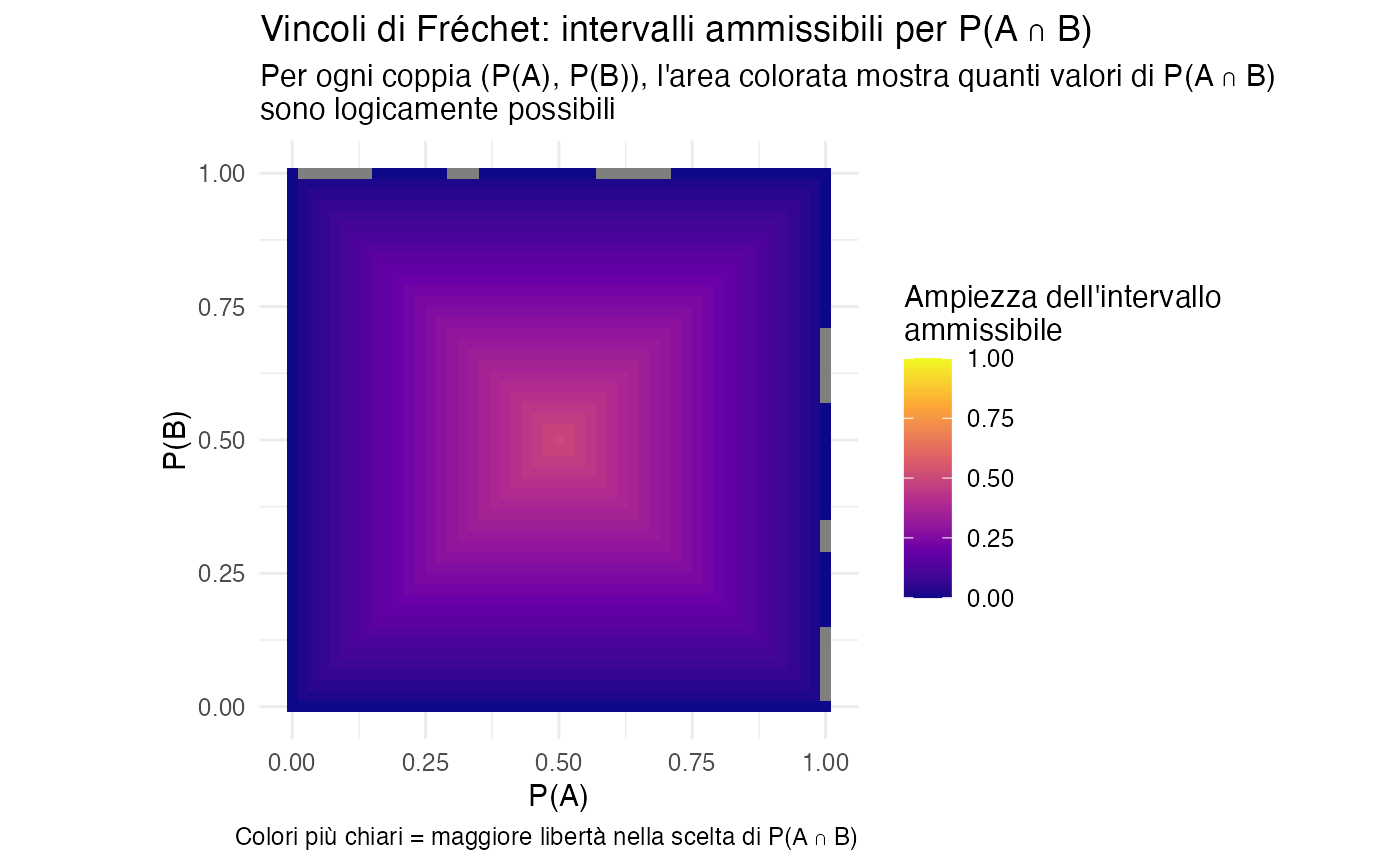
\includegraphics[width=1\linewidth,height=\textheight,keepaspectratio]{chapters/probability/02_axioms_coherence_bayesian_files/figure-pdf/unnamed-chunk-2-1.png}

}

\caption{Regione dei valori ammissibili per P(A ∩ B) in funzione di P(A)
e P(B).}

\end{figure}%

La mappa rivela pattern interessanti. Negli angoli, corrispondenti agli
eventi rari o quasi certi, i vincoli sono stringenti e c'è poca libertà
nella scelta della probabilità congiunta. Al centro, dove le probabilità
sono intermedie, c'è più libertà.

La regione in alto a destra, in cui \(P(A) + P(B) > 1\), impone una
sovrapposizione minima obbligatoria. La regione in basso a sinistra
permette una sovrapposizione nulla.

\end{tcolorbox}

\section{Tabelle di probabilità
congiunta}\label{tabelle-di-probabilituxe0-congiunta}

Passiamo ora dallo studio dei vincoli teorici alla costruzione di
rappresentazioni operative. Le \textbf{tabelle di probabilità congiunta}
sono lo strumento fondamentale per questo scopo.

\subsection{L'idea centrale: la distribuzione congiunta è la
``fonte''}\label{lidea-centrale-la-distribuzione-congiunta-uxe8-la-fonte}

Quando abbiamo due o più variabili, possiamo chiederci:

\begin{itemize}
\tightlist
\item
  Qual è la probabilità di ciascun valore della prima variabile?
  (\emph{marginale})
\item
  Qual è la probabilità di ciascuna \emph{combinazione} di valori?
  (\emph{congiunta})
\item
  Se conosco il valore di una variabile, qual è la probabilità dei
  valori dell'altra? (\emph{condizionata})
\end{itemize}

Queste domande non sono indipendenti. Se conosco la distribuzione
congiunta --- ovvero le probabilità di tutte le combinazioni --- posso
\textbf{derivare} tutte le altre. La distribuzione congiunta è come il
DNA del sistema: contiene tutte le informazioni; marginali e
condizionate sono caratteristiche che emergono da quel DNA.

\subsection{Struttura di una tabella
2×2}\label{struttura-di-una-tabella-22}

Consideriamo il caso più semplice: due eventi dicotomici \(A\) e \(B\).

{\def\LTcaptype{none} % do not increment counter
\begin{longtable}[]{@{}llll@{}}
\toprule\noalign{}
& \(B\) & \(B^c\) & Marginale \\
\midrule\noalign{}
\endhead
\bottomrule\noalign{}
\endlastfoot
\(A\) & \(P(A \cap B)\) & \(P(A \cap B^c)\) & \(P(A)\) \\
\(A^c\) & \(P(A^c \cap B)\) & \(P(A^c \cap B^c)\) & \(P(A^c)\) \\
\textbf{Marginale} & \(P(B)\) & \(P(B^c)\) & \(1\) \\
\end{longtable}
}

\begin{itemize}
\tightlist
\item
  Le \textbf{quattro celle interne} contengono le probabilità congiunte.
\item
  I \textbf{margini} contengono le probabilità marginali, ottenute
  sommando righe o colonne:
\end{itemize}

\[P(A) = P(A \cap B) + P(A \cap B^c), \qquad P(B) = P(A \cap B) + P(A^c \cap B).\]

\begin{itemize}
\tightlist
\item
  L'\textbf{angolo in basso a destra} deve valere 1: la somma di tutte
  le celle (e di tutte le marginali) è 1.
\end{itemize}

\subsection{Costruzione di una tabella
congiunta}\label{costruzione-di-una-tabella-congiunta}

Come si costruisce una tabella congiunta a partire dalle informazioni
disponibili? La regola fondamentale è il \textbf{principio del
prodotto}:

\[P(A \cap B) = P(A \mid B) \, P(B) = P(B \mid A) \, P(A).\]

Se conosciamo una probabilità marginale e una condizionata, possiamo
ricavare la congiunta.

\begin{tcolorbox}[enhanced jigsaw, arc=.35mm, bottomrule=.15mm, bottomtitle=1mm, breakable, colback=white, colbacktitle=quarto-callout-note-color!10!white, colframe=quarto-callout-note-color-frame, coltitle=black, left=2mm, leftrule=.75mm, opacityback=0, opacitybacktitle=0.6, rightrule=.15mm, title=\textcolor{quarto-callout-note-color}{\faInfo}\hspace{0.5em}{Esempio: test diagnostico per la depressione}, titlerule=0mm, toprule=.15mm, toptitle=1mm]

Consideriamo un test per la depressione con:

\begin{itemize}
\tightlist
\item
  \textbf{prevalenza}: \(P(D) = 0.15\);
\item
  \textbf{sensibilità}: \(P(T^+ \mid D) = 0.85\);
\item
  \textbf{tasso di falsi positivi}: \(P(T^+ \mid D^c) = 0.20\).
\end{itemize}

Costruiamo la tabella congiunta:

\begin{Shaded}
\begin{Highlighting}[]
\NormalTok{prevalenza }\OtherTok{\textless{}{-}} \FloatTok{0.15}
\NormalTok{sensibilita }\OtherTok{\textless{}{-}} \FloatTok{0.85}
\NormalTok{tasso\_falsi\_positivi }\OtherTok{\textless{}{-}} \FloatTok{0.20}

\NormalTok{p\_D\_pos }\OtherTok{\textless{}{-}}\NormalTok{ sensibilita }\SpecialCharTok{*}\NormalTok{ prevalenza          }\CommentTok{\# 0.1275}
\NormalTok{p\_D\_neg }\OtherTok{\textless{}{-}}\NormalTok{ (}\DecValTok{1} \SpecialCharTok{{-}}\NormalTok{ sensibilita) }\SpecialCharTok{*}\NormalTok{ prevalenza    }\CommentTok{\# 0.0225}
\NormalTok{p\_Dc\_pos }\OtherTok{\textless{}{-}}\NormalTok{ tasso\_falsi\_positivi }\SpecialCharTok{*}\NormalTok{ (}\DecValTok{1} \SpecialCharTok{{-}}\NormalTok{ prevalenza)   }\CommentTok{\# 0.1700}
\NormalTok{p\_Dc\_neg }\OtherTok{\textless{}{-}}\NormalTok{ (}\DecValTok{1} \SpecialCharTok{{-}}\NormalTok{ tasso\_falsi\_positivi) }\SpecialCharTok{*}\NormalTok{ (}\DecValTok{1} \SpecialCharTok{{-}}\NormalTok{ prevalenza) }\CommentTok{\# 0.6800}

\NormalTok{tabella\_congiunta }\OtherTok{\textless{}{-}} \FunctionTok{matrix}\NormalTok{(}
  \FunctionTok{c}\NormalTok{(p\_D\_pos, p\_D\_neg, p\_Dc\_pos, p\_Dc\_neg),}
  \AttributeTok{nrow =} \DecValTok{2}\NormalTok{, }\AttributeTok{byrow =} \ConstantTok{TRUE}\NormalTok{,}
  \AttributeTok{dimnames =} \FunctionTok{list}\NormalTok{(}
    \StringTok{"Stato reale"} \OtherTok{=} \FunctionTok{c}\NormalTok{(}\StringTok{"Depresso"}\NormalTok{, }\StringTok{"Non depresso"}\NormalTok{),}
    \StringTok{"Test"} \OtherTok{=} \FunctionTok{c}\NormalTok{(}\StringTok{"Positivo"}\NormalTok{, }\StringTok{"Negativo"}\NormalTok{)}
\NormalTok{  )}
\NormalTok{)}
\FunctionTok{round}\NormalTok{(tabella\_congiunta, }\DecValTok{4}\NormalTok{)}
\CommentTok{\#\textgreater{}               Test}
\CommentTok{\#\textgreater{} Stato reale    Positivo Negativo}
\CommentTok{\#\textgreater{}   Depresso        0.128   0.0225}
\CommentTok{\#\textgreater{}   Non depresso    0.170   0.6800}
\end{Highlighting}
\end{Shaded}

Ogni cella rappresenta la probabilità di una combinazione: veri positivi
(0.1275), falsi negativi (0.0225), falsi positivi (0.1700), veri
negativi (0.6800). La somma è 1.

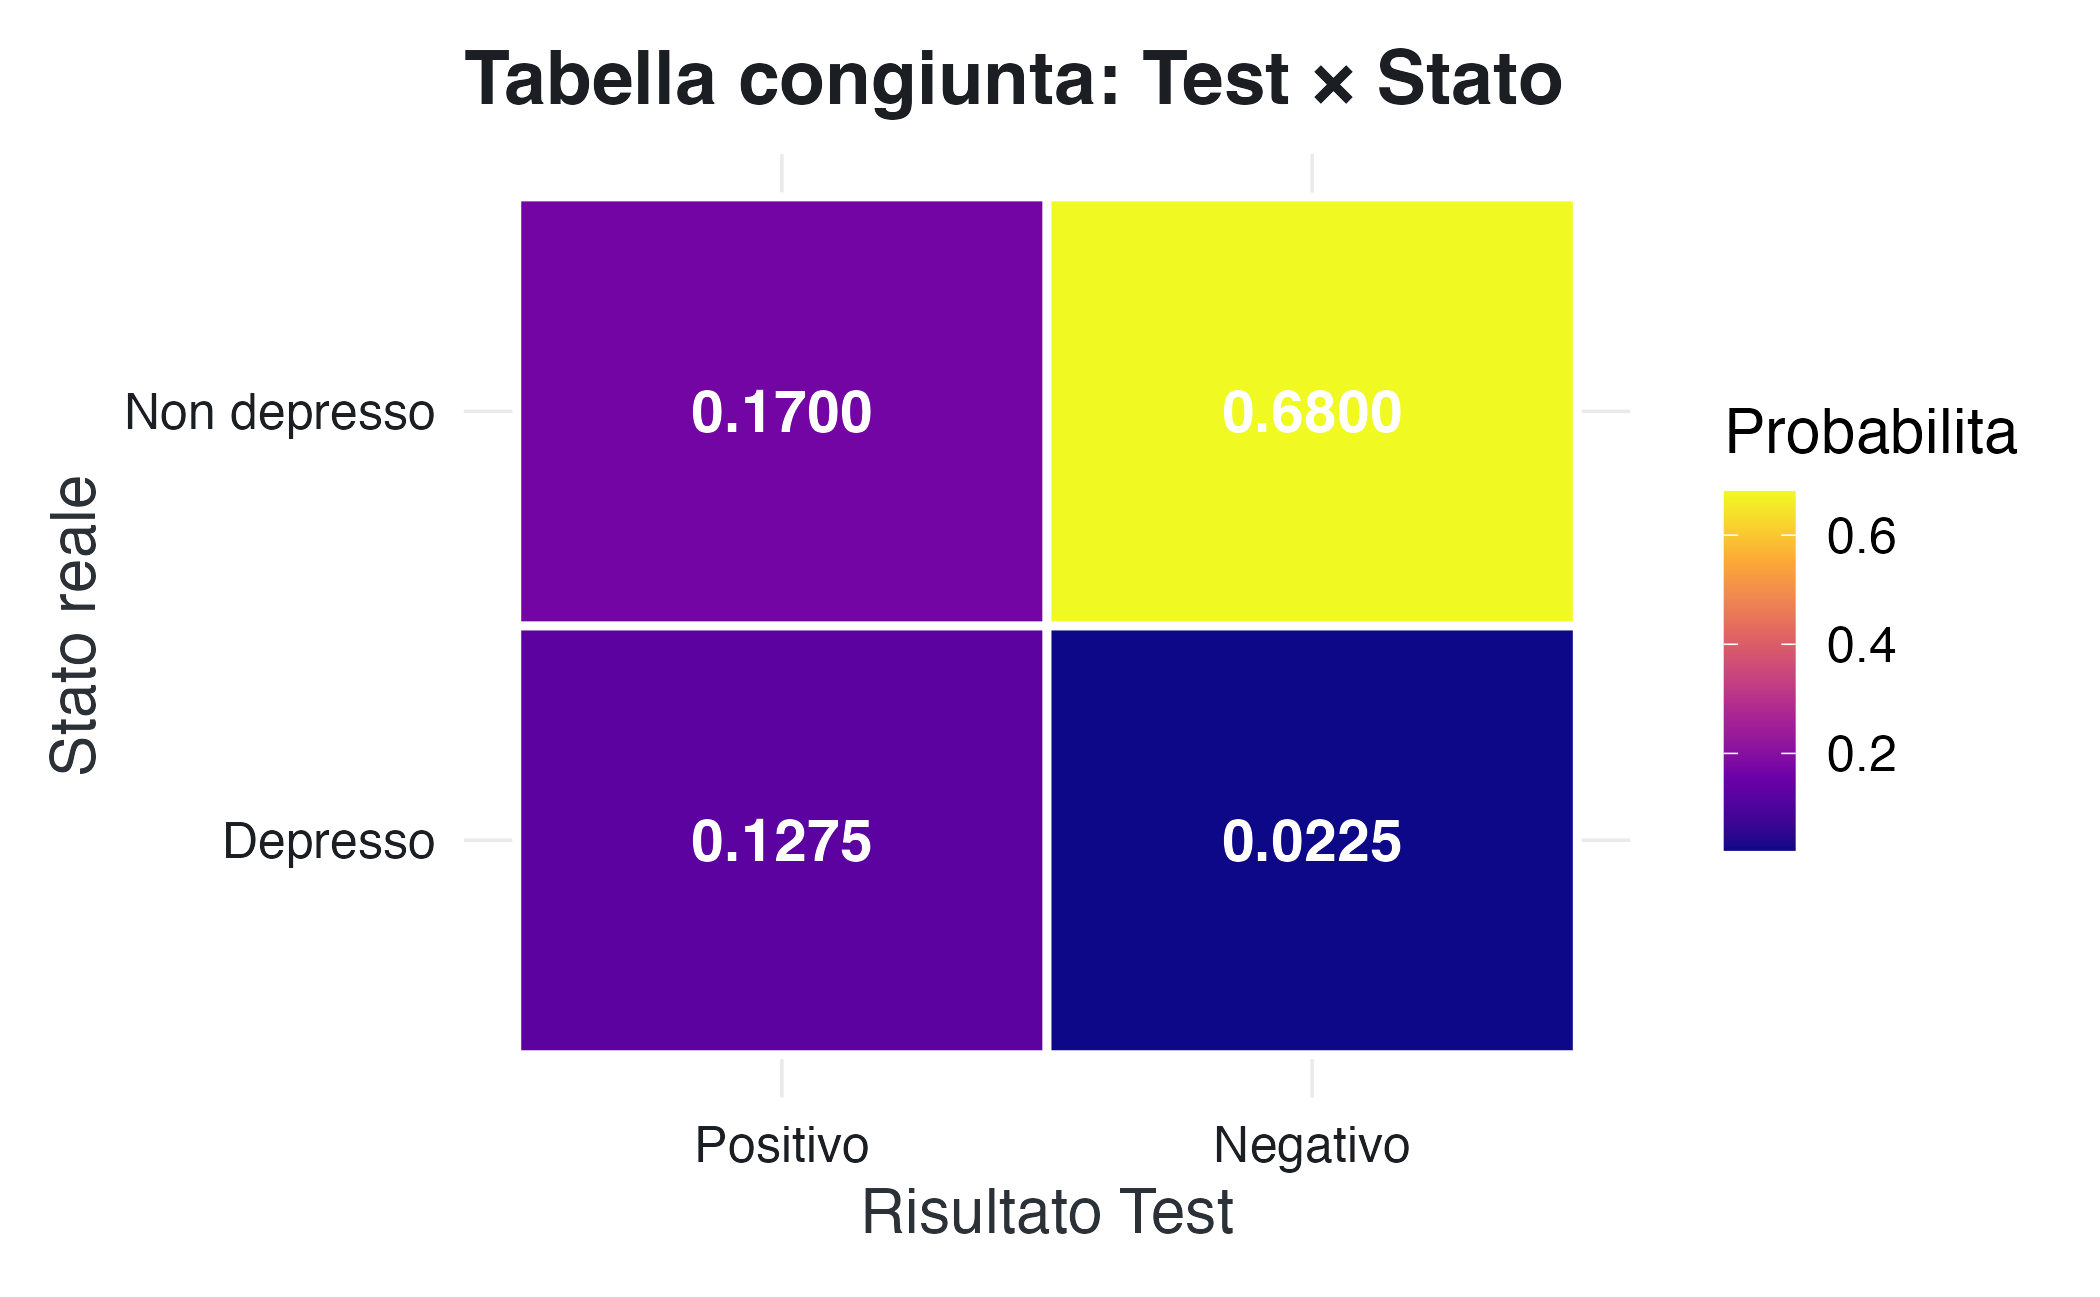
\includegraphics[width=0.85\linewidth,height=\textheight,keepaspectratio]{chapters/probability/02_axioms_coherence_bayesian_files/figure-pdf/unnamed-chunk-4-1.png}

\end{tcolorbox}

\subsection{Calcolo di marginali e
condizionate}\label{calcolo-di-marginali-e-condizionate}

Una volta costruita la tabella congiunta, tutto il resto si ottiene per
derivazione.

\subsubsection{Probabilità marginali}\label{probabilituxe0-marginali}

Si ottengono sommando lungo righe o colonne:

\begin{verbatim}
#> P(D)     = 0.15 (prevalenza)
#> P(T+)    = 0.297 (test positivo)
\end{verbatim}

Notiamo che \(P(T^+) \approx 0.30\) è molto più alta della prevalenza
(0.15), perché include sia i veri che i falsi positivi.

\subsubsection{Probabilità
condizionate}\label{probabilituxe0-condizionate}

Si ottengono come rapporto tra probabilità congiunta e marginale:

\[P(A \mid B) = \frac{P(A \cap B)}{P(B)}.\]

\textbf{Interpretazione epistemica}: condizionare significa
\emph{restringere} lo spazio delle possibilità a quelle compatibili con
l'informazione acquisita, ri-normalizzando le probabilità su questo
spazio ristretto.

\begin{tcolorbox}[enhanced jigsaw, arc=.35mm, bottomrule=.15mm, bottomtitle=1mm, breakable, colback=white, colbacktitle=quarto-callout-note-color!10!white, colframe=quarto-callout-note-color-frame, coltitle=black, left=2mm, leftrule=.75mm, opacityback=0, opacitybacktitle=0.6, rightrule=.15mm, title=\textcolor{quarto-callout-note-color}{\faInfo}\hspace{0.5em}{Esempio: valore predittivo positivo}, titlerule=0mm, toprule=.15mm, toptitle=1mm]

La domanda clinica cruciale: ``Se il test è positivo, qual è la
probabilità che il paziente sia depresso?''

\[P(D \mid T^+) = \frac{P(D \cap T^+)}{P(T^+)} = \frac{0.1275}{0.1275 + 0.1700} \approx 0.429.\]

\begin{verbatim}
#> P(D | T+) = 0.429
\end{verbatim}

Nonostante l'85\% di sensibilità, un test positivo indica depressione
solo nel 43\% dei casi. La ragione è la bassa prevalenza: la maggior
parte dei positivi è falsa. Questo fenomeno, il \emph{paradosso dei test
diagnostici}, è stato introdotto nel capitolo precedente e sarà ripreso
nel Capitolo~\ref{sec-prob-bayes-theorem}.

\end{tcolorbox}

\begin{tcolorbox}[enhanced jigsaw, arc=.35mm, bottomrule=.15mm, bottomtitle=1mm, breakable, colback=white, colbacktitle=quarto-callout-important-color!10!white, colframe=quarto-callout-important-color-frame, coltitle=black, left=2mm, leftrule=.75mm, opacityback=0, opacitybacktitle=0.6, rightrule=.15mm, title=\textcolor{quarto-callout-important-color}{\faExclamation}\hspace{0.5em}{Messaggio chiave}, titlerule=0mm, toprule=.15mm, toptitle=1mm]

Una volta specificata la tabella congiunta, marginali e condizionate
sono \textbf{determinate}. Non c'è libertà di scelta: specificare
separatamente \(P(A \mid B)\) e \(P(B \mid A)\) senza una congiunta
coerente quasi certamente introduce contraddizioni.

La regola è: \textbf{specificare la distribuzione congiunta, derivare
tutto il resto}.

\end{tcolorbox}

\subsection{Verifica empirica mediante
simulazione}\label{verifica-empirica-mediante-simulazione}

Un modo potente per verificare la coerenza di un sistema di credenze è
simulare dati secondo quella distribuzione e controllare che le
frequenze osservate convergano alle probabilità teoriche.

\begin{tcolorbox}[enhanced jigsaw, arc=.35mm, bottomrule=.15mm, bottomtitle=1mm, breakable, colback=white, colbacktitle=quarto-callout-note-color!10!white, colframe=quarto-callout-note-color-frame, coltitle=black, left=2mm, leftrule=.75mm, opacityback=0, opacitybacktitle=0.6, rightrule=.15mm, title=\textcolor{quarto-callout-note-color}{\faInfo}\hspace{0.5em}{Verifica Monte Carlo}, titlerule=0mm, toprule=.15mm, toptitle=1mm]

Simuliamo 100.000 osservazioni dalla tabella congiunta:

\begin{Shaded}
\begin{Highlighting}[]
\FunctionTok{set.seed}\NormalTok{(}\DecValTok{123}\NormalTok{)}
\NormalTok{N }\OtherTok{\textless{}{-}} \DecValTok{100000}
\NormalTok{probs }\OtherTok{\textless{}{-}} \FunctionTok{c}\NormalTok{(p\_D\_pos, p\_D\_neg, p\_Dc\_pos, p\_Dc\_neg)}
\NormalTok{outcomes }\OtherTok{\textless{}{-}} \FunctionTok{sample}\NormalTok{(}\DecValTok{1}\SpecialCharTok{:}\DecValTok{4}\NormalTok{, }\AttributeTok{size =}\NormalTok{ N, }\AttributeTok{replace =} \ConstantTok{TRUE}\NormalTok{, }\AttributeTok{prob =}\NormalTok{ probs)}
\NormalTok{freq\_empiriche }\OtherTok{\textless{}{-}} \FunctionTok{table}\NormalTok{(outcomes) }\SpecialCharTok{/}\NormalTok{ N}

\NormalTok{df\_verifica }\OtherTok{\textless{}{-}} \FunctionTok{data.frame}\NormalTok{(}
  \AttributeTok{Configurazione =} \FunctionTok{c}\NormalTok{(}\StringTok{"D∩T+"}\NormalTok{, }\StringTok{"D∩T{-}"}\NormalTok{, }\StringTok{"D\^{}c∩T+"}\NormalTok{, }\StringTok{"D\^{}c∩T{-}"}\NormalTok{),}
  \AttributeTok{Teorica =} \FunctionTok{round}\NormalTok{(probs, }\DecValTok{4}\NormalTok{),}
  \AttributeTok{Empirica =} \FunctionTok{round}\NormalTok{(}\FunctionTok{as.numeric}\NormalTok{(freq\_empiriche), }\DecValTok{4}\NormalTok{)}
\NormalTok{)}
\FunctionTok{print}\NormalTok{(df\_verifica)}
\CommentTok{\#\textgreater{}   Configurazione Teorica Empirica}
\CommentTok{\#\textgreater{} 1           D∩T+  0.1275   0.1266}
\CommentTok{\#\textgreater{} 2           D∩T{-}  0.0225   0.0226}
\CommentTok{\#\textgreater{} 3         D\^{}c∩T+  0.1700   0.1699}
\CommentTok{\#\textgreater{} 4         D\^{}c∩T{-}  0.6800   0.6809}
\end{Highlighting}
\end{Shaded}

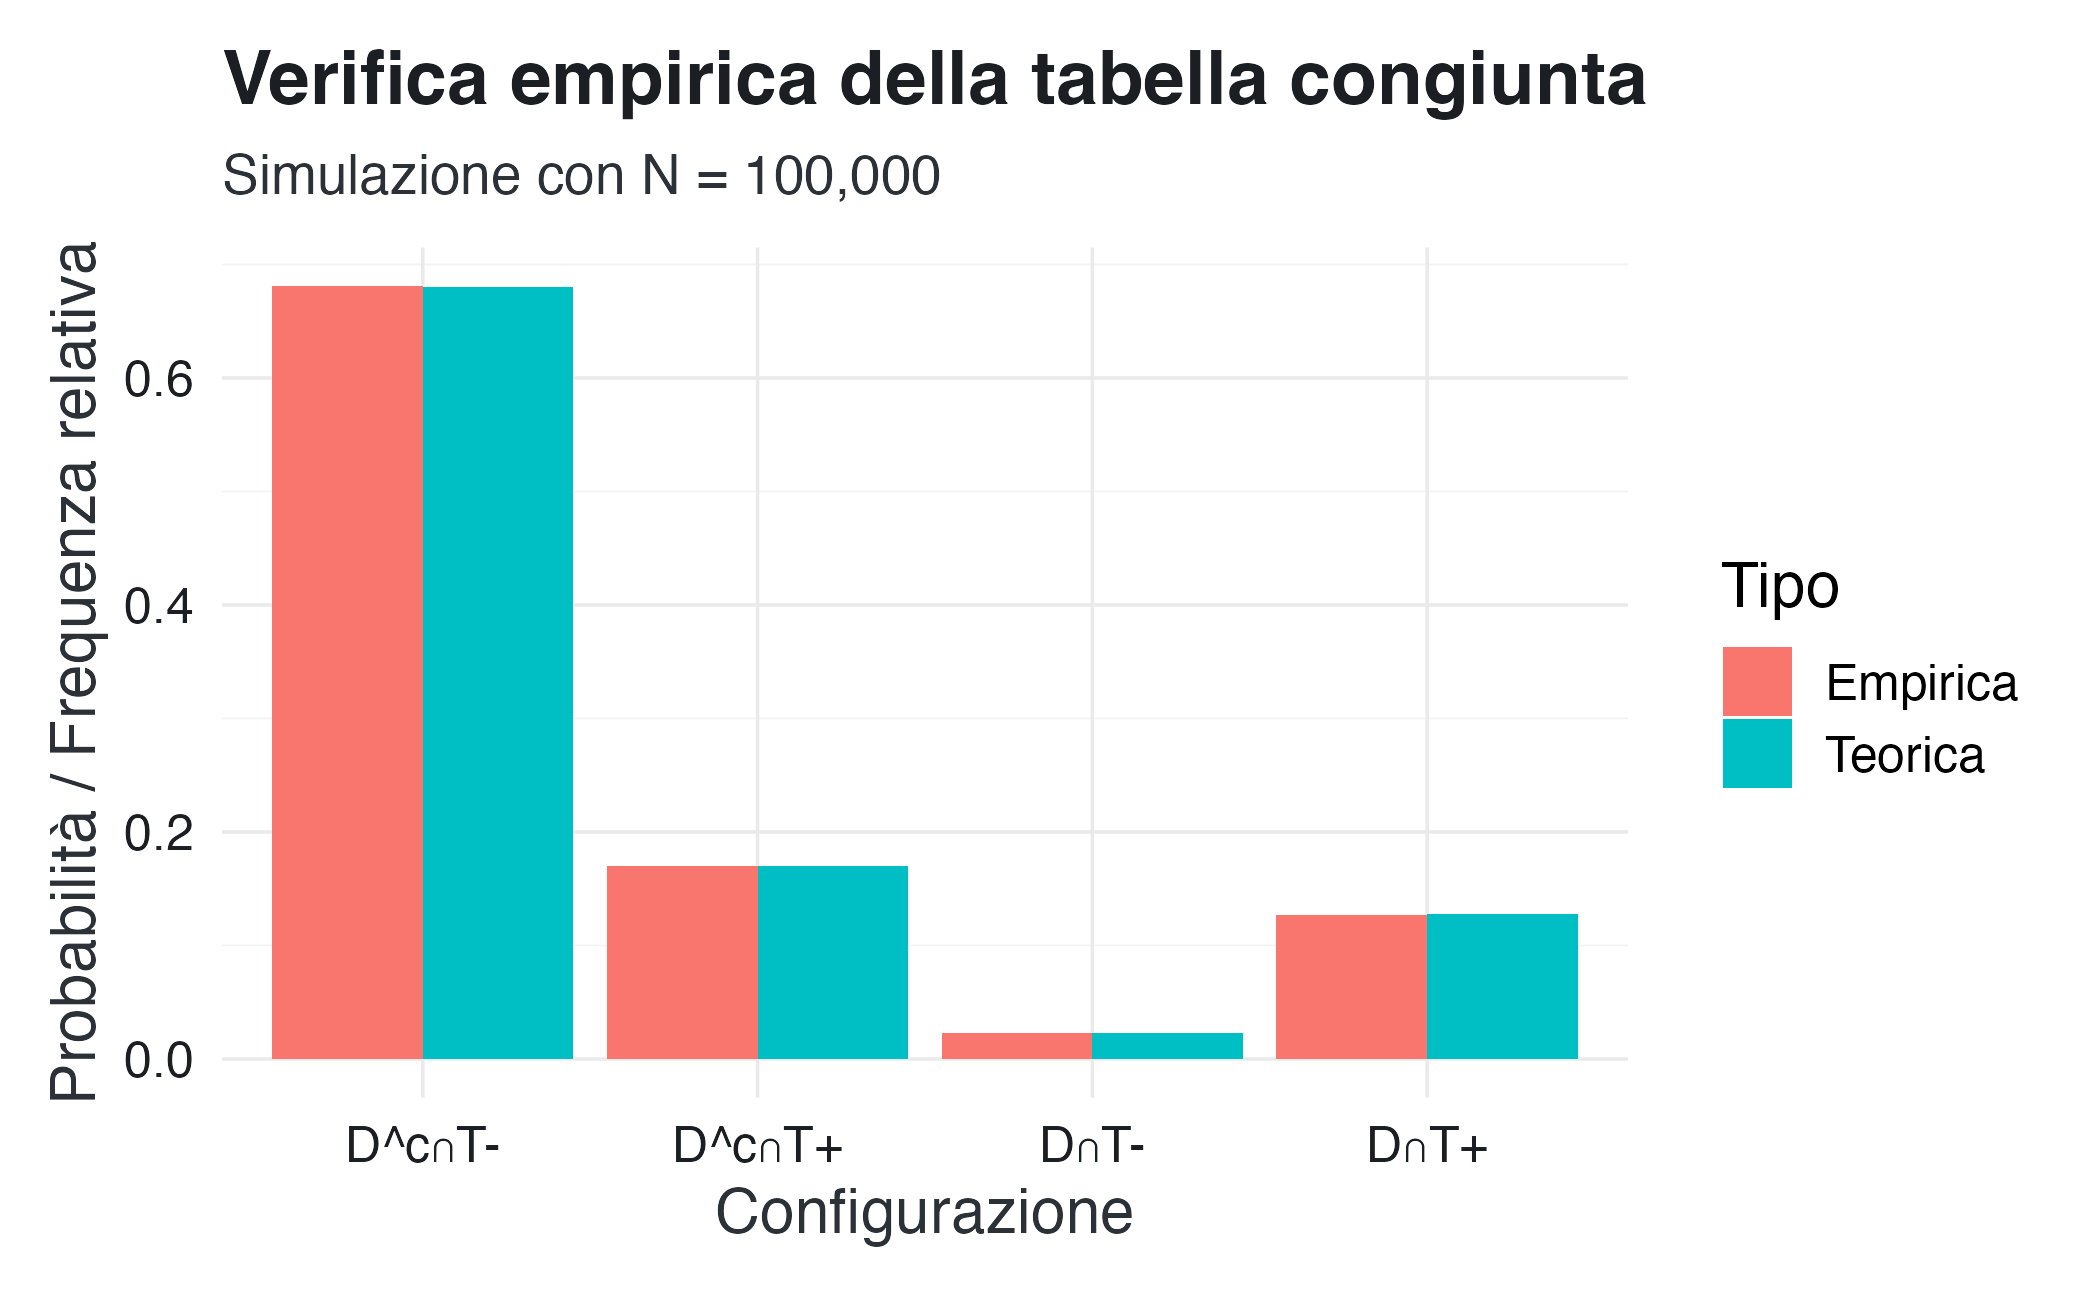
\includegraphics[width=0.85\linewidth,height=\textheight,keepaspectratio]{chapters/probability/02_axioms_coherence_bayesian_files/figure-pdf/unnamed-chunk-8-1.png}

La convergenza delle frequenze empiriche verso le probabilità teoriche
conferma che la distribuzione congiunta è un sistema coerente che
specifica un \emph{modello generativo} del mondo.

\end{tcolorbox}

\subsection{Estensione a tabelle
multidimensionali}\label{estensione-a-tabelle-multidimensionali}

Il framework si estende naturalmente a più variabili e più categorie. Il
principio è invariato: specificare le probabilità di tutte le
combinazioni, derivare tutto il resto.

\begin{tcolorbox}[enhanced jigsaw, arc=.35mm, bottomrule=.15mm, bottomtitle=1mm, breakable, colback=white, colbacktitle=quarto-callout-note-color!10!white, colframe=quarto-callout-note-color-frame, coltitle=black, left=2mm, leftrule=.75mm, opacityback=0, opacitybacktitle=0.6, rightrule=.15mm, title=\textcolor{quarto-callout-note-color}{\faInfo}\hspace{0.5em}{Esempio: depressione × ansia (tabella 2×3)}, titlerule=0mm, toprule=.15mm, toptitle=1mm]

\begin{Shaded}
\begin{Highlighting}[]
\NormalTok{tab\_2x3 }\OtherTok{\textless{}{-}} \FunctionTok{matrix}\NormalTok{(}
  \FunctionTok{c}\NormalTok{(}\FloatTok{0.15}\NormalTok{, }\FloatTok{0.20}\NormalTok{, }\FloatTok{0.15}\NormalTok{,  }\CommentTok{\# Depresso: ansia nessuna/lieve/grave}
    \FloatTok{0.35}\NormalTok{, }\FloatTok{0.10}\NormalTok{, }\FloatTok{0.05}\NormalTok{), }\CommentTok{\# Non depresso: ansia nessuna/lieve/grave}
  \AttributeTok{nrow =} \DecValTok{2}\NormalTok{, }\AttributeTok{byrow =} \ConstantTok{TRUE}\NormalTok{,}
  \AttributeTok{dimnames =} \FunctionTok{list}\NormalTok{(}
    \AttributeTok{Depressione =} \FunctionTok{c}\NormalTok{(}\StringTok{"D"}\NormalTok{, }\StringTok{"D\^{}c"}\NormalTok{),}
    \AttributeTok{Ansia =} \FunctionTok{c}\NormalTok{(}\StringTok{"Nessuna"}\NormalTok{, }\StringTok{"Lieve"}\NormalTok{, }\StringTok{"Grave"}\NormalTok{)}
\NormalTok{  )}
\NormalTok{)}
\FunctionTok{print}\NormalTok{(tab\_2x3)}
\CommentTok{\#\textgreater{}            Ansia}
\CommentTok{\#\textgreater{} Depressione Nessuna Lieve Grave}
\CommentTok{\#\textgreater{}         D      0.15   0.2  0.15}
\CommentTok{\#\textgreater{}         D\^{}c    0.35   0.1  0.05}
\FunctionTok{cat}\NormalTok{(}\StringTok{"}\SpecialCharTok{\textbackslash{}n}\StringTok{Marginali depressione:"}\NormalTok{, }\FunctionTok{rowSums}\NormalTok{(tab\_2x3), }\StringTok{"}\SpecialCharTok{\textbackslash{}n}\StringTok{"}\NormalTok{)}
\CommentTok{\#\textgreater{} }
\CommentTok{\#\textgreater{} Marginali depressione: 0.5 0.5}
\FunctionTok{cat}\NormalTok{(}\StringTok{"Marginali ansia:"}\NormalTok{, }\FunctionTok{colSums}\NormalTok{(tab\_2x3), }\StringTok{"}\SpecialCharTok{\textbackslash{}n}\StringTok{"}\NormalTok{)}
\CommentTok{\#\textgreater{} Marginali ansia: 0.5 0.3 0.2}
\end{Highlighting}
\end{Shaded}

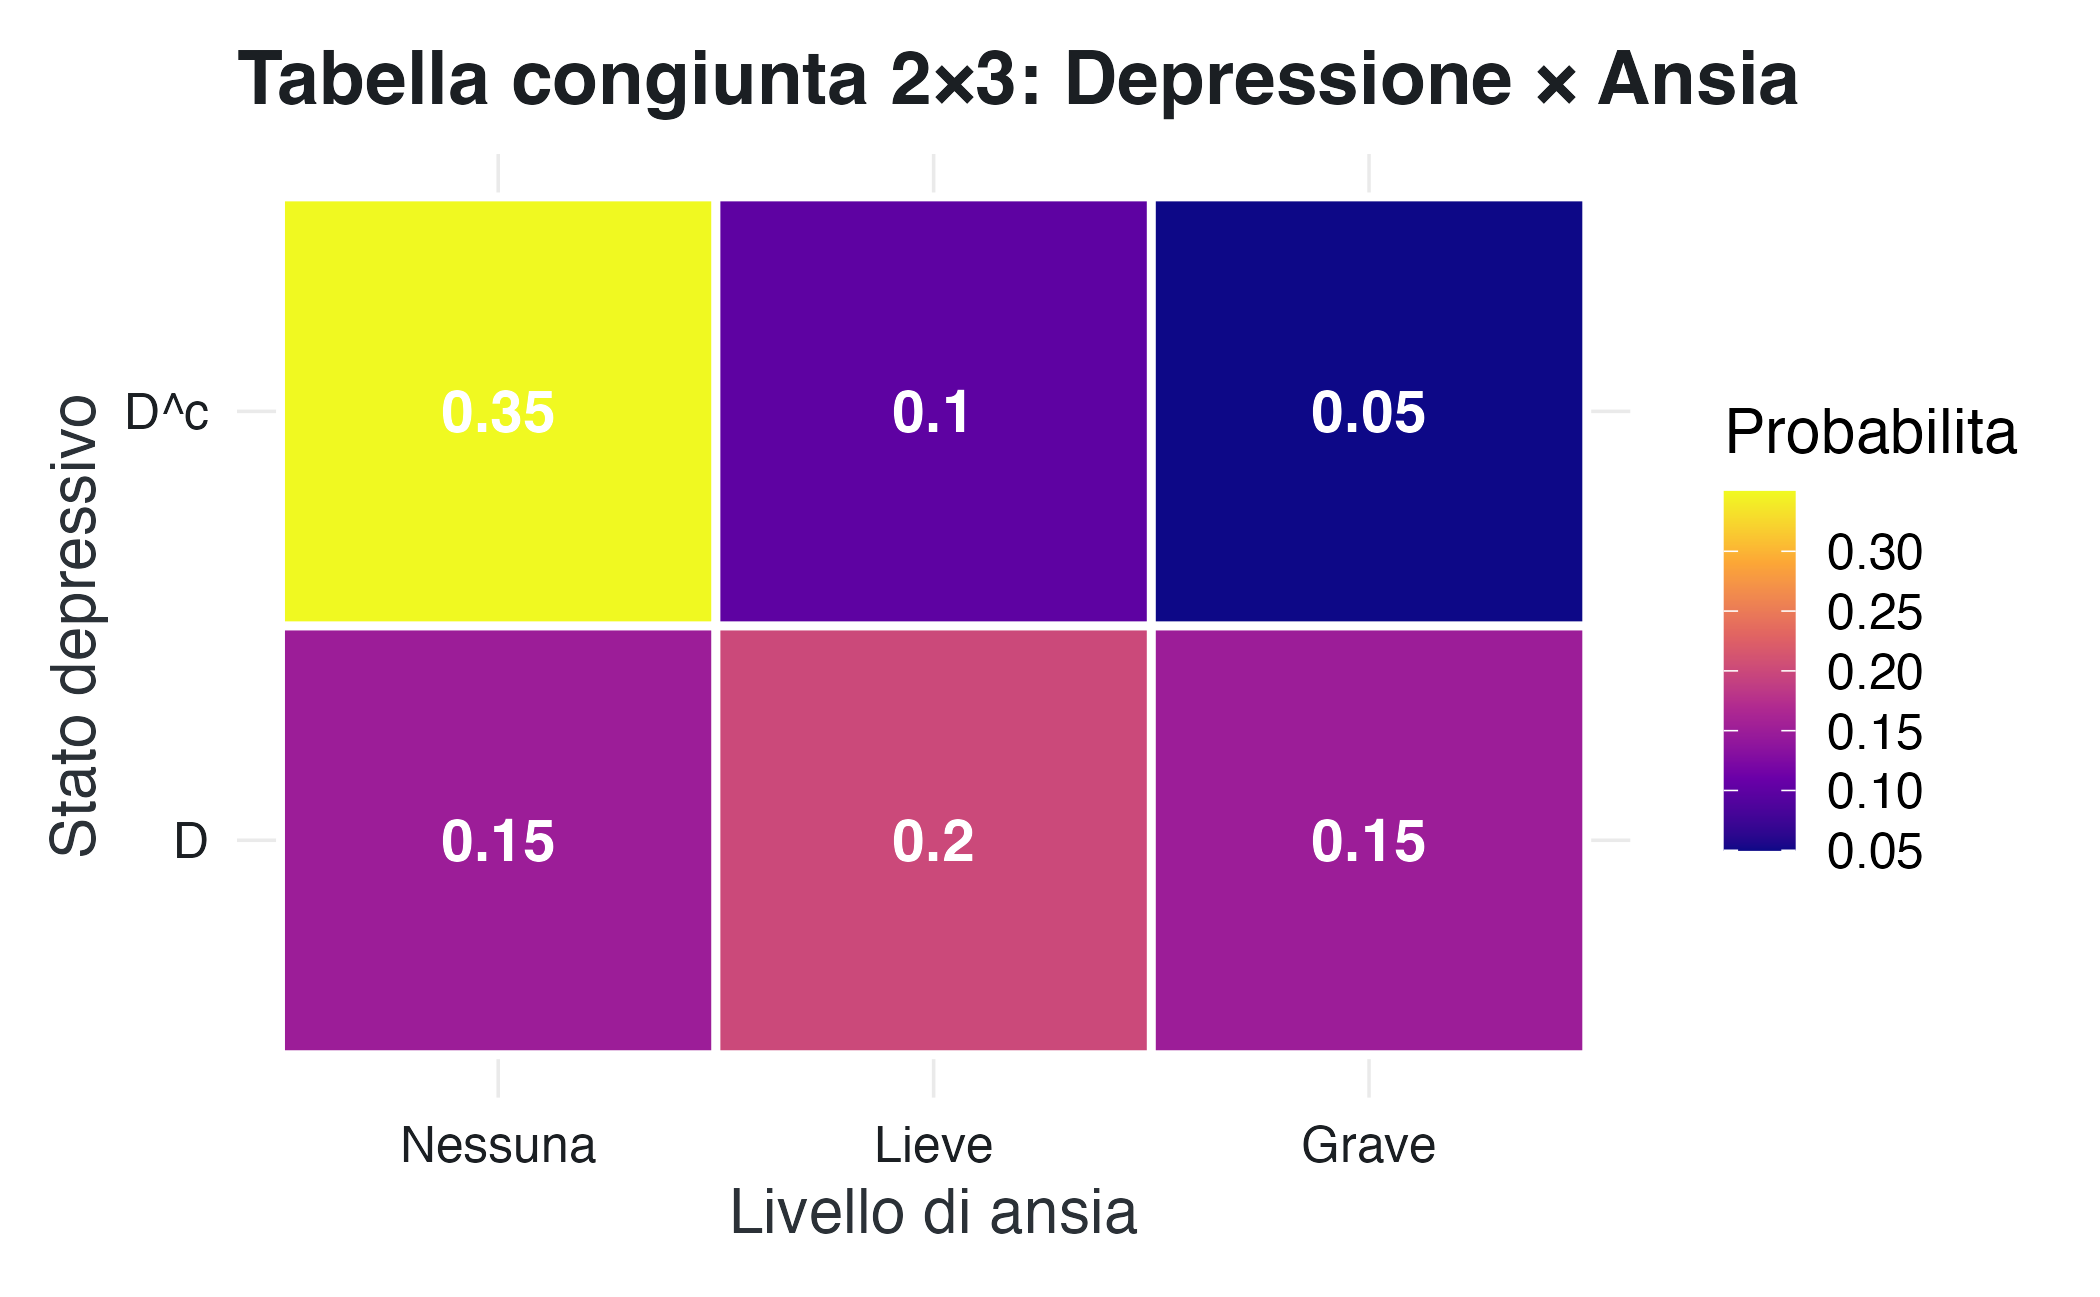
\includegraphics[width=0.85\linewidth,height=\textheight,keepaspectratio]{chapters/probability/02_axioms_coherence_bayesian_files/figure-pdf/unnamed-chunk-10-1.png}

\end{tcolorbox}

\section*{Riflessioni conclusive}\label{riflessioni-conclusive-1}

\markright{Riflessioni conclusive}

Siamo partiti da una domanda apparentemente astratta: cosa significa che
le credenze siano ``coerenti''? e siamo arrivati a strumenti concreti
per rappresentare e manipolare sistemi di credenze complessi.

Il percorso ha rivelato che la matematica della probabilità non è un
formalismo arbitrario, ma la \textbf{struttura logica necessaria} per
ragionare in modo coerente in situazioni di incertezza. Gli assiomi di
Kolmogorov non sono delle semplici convenzioni, ma dei vincoli che
\textbf{dobbiamo rispettare} se vogliamo evitare contraddizioni.

\subsection{Cosa abbiamo guadagnato}\label{cosa-abbiamo-guadagnato}

Per lo psicologo, questo framework offre diversi vantaggi:

\begin{enumerate}
\def\labelenumi{\arabic{enumi}.}
\item
  \textbf{Uno standard normativo}: ora sappiamo cosa significa che un
  giudizio probabilistico sia ``corretto'' dal punto di vista logico,
  anche se può essere sbagliato dal punto di vista empirico.
\item
  \textbf{Strumenti diagnostici}: possiamo identificare incoerenze nei
  ragionamenti (nostri e altrui) utilizzando criteri precisi, come i
  vincoli di Fréchet.
\item
  \textbf{Una rappresentazione unificata}: le tabelle di probabilità
  congiunta condensano in un'unica struttura tutte le informazioni
  probabilistiche rilevanti su un sistema.
\item
  \textbf{Un ponte verso i dati}: la connessione tra probabilità
  teoriche e simulazioni mostra come le nostre credenze si traducano in
  aspettative sui dati osservabili.
\end{enumerate}

\subsection{Cosa manca ancora}\label{cosa-manca-ancora}

Questo capitolo ha gettato le basi, ma restano ancora delle domande
senza risposta:

\begin{itemize}
\tightlist
\item
  Come assegnare le probabilità \emph{iniziali} quando non abbiamo dati?
  (Tema dell'equiprobabilità).
\item
  Come \emph{aggiorniamo} le nostre credenze quando osserviamo nuove
  evidenze? (Teorema di Bayes).
\item
  Come trattiamo variabili \emph{continue} che non rientrano in tabelle
  discrete? (Distribuzioni di probabilità).
\end{itemize}

Questi temi verranno sviluppati nei capitoli successivi. Tuttavia, la
struttura di coerenza che abbiamo costruito rimarrà la cornice di
riferimento.

\subsection{Un invito alla
riflessione}\label{un-invito-alla-riflessione}

Prima di procedere, è opportuno soffermarsi a considerare un punto
filosofico più profondo. Abbiamo visto che la coerenza è
\emph{necessaria} per evitare contraddizioni. Ma è \emph{sufficiente}
per ragionare bene?

La risposta è no. Un sistema di credenze può essere perfettamente
coerente ma completamente errato. Posso credere con certezza matematica
che domani pioveranno pesci dal cielo, e queste credenze possono essere
internamente coerenti, ma saranno smentite dalla realtà.

La coerenza è una condizione \emph{minima}, non una garanzia di verità.
Ci protegge dagli errori logici, ma non da quelli empirici. Per
avvicinarci alla verità, dobbiamo anche confrontare le nostre credenze
con i dati, e questo sarà il tema dell'\textbf{inferenza bayesiana}.

\section*{Punti chiave da ricordare}\label{punti-chiave-da-ricordare-1}
\addcontentsline{toc}{section}{Punti chiave da ricordare}

\markright{Punti chiave da ricordare}

\begin{tcolorbox}[enhanced jigsaw, arc=.35mm, bottomrule=.15mm, bottomtitle=1mm, breakable, colback=white, colbacktitle=quarto-callout-important-color!10!white, colframe=quarto-callout-important-color-frame, coltitle=black, left=2mm, leftrule=.75mm, opacityback=0, opacitybacktitle=0.6, rightrule=.15mm, title=\textcolor{quarto-callout-important-color}{\faExclamation}\hspace{0.5em}{Importante}, titlerule=0mm, toprule=.15mm, toptitle=1mm]

\textbf{Concetti essenziali di questo capitolo:}

\begin{enumerate}
\def\labelenumi{\arabic{enumi}.}
\item
  \textbf{I tre assiomi di Kolmogorov}

  \begin{itemize}
  \tightlist
  \item
    Non-negatività: \(P(A) \geq 0\) per ogni evento \(A\).
  \item
    Normalizzazione: \(P(\Omega) = 1\) (certezza per l'intero spazio
    campionario).
  \item
    Additività: \(P(A \cup B) = P(A) + P(B)\) se \(A\) e \(B\) sono
    disgiunti.
  \end{itemize}
\item
  \textbf{Principio di coerenza}

  \begin{itemize}
  \tightlist
  \item
    Le credenze probabilistiche devono essere internamente consistenti.
  \item
    Un sistema di credenze incoerente porta a perdite certe (Dutch book
    argument).
  \item
    Gli assiomi \emph{garantiscono} la coerenza razionale delle nostre
    valutazioni.
  \end{itemize}
\item
  \textbf{Conseguenze degli assiomi}

  \begin{itemize}
  \tightlist
  \item
    Probabilità del complemento: \(P(A^c) = 1 - P(A)\).
  \item
    Evento impossibile: \(P(\emptyset) = 0\).
  \item
    Regola dell'unione generale:
    \(P(A \cup B) = P(A) + P(B) - P(A \cap B)\).
  \end{itemize}
\item
  \textbf{Tabelle di probabilità congiunta}

  \begin{itemize}
  \tightlist
  \item
    Contengono l'informazione completa sul sistema.
  \item
    Marginali = somme di righe/colonne.
  \item
    Condizionate = rapporti (congiunta / marginale).
  \item
    Tutto deriva dalla distribuzione congiunta.
  \end{itemize}
\end{enumerate}

\textbf{Formule da ricordare:}

\[P(A^c) = 1 - P(A)\]

\[P(A \cup B) = P(A) + P(B) - P(A \cap B)\]

\[P(A \mid B) = \frac{P(A \cap B)}{P(B)}\]

\textbf{Per il prossimo capitolo:}

Nel Capitolo~\ref{sec-equiprobability-combinatorics} vedremo come
applicare questi assiomi a situazioni di equiprobabilità, introducendo
il calcolo combinatorio per contare i casi favorevoli e possibili.

\end{tcolorbox}

\section*{Esercizi}\label{esercizi}

\markright{Esercizi}

\begin{tcolorbox}[enhanced jigsaw, arc=.35mm, bottomrule=.15mm, bottomtitle=1mm, breakable, colback=white, colbacktitle=quarto-callout-important-color!10!white, colframe=quarto-callout-important-color-frame, coltitle=black, left=2mm, leftrule=.75mm, opacityback=0, opacitybacktitle=0.6, rightrule=.15mm, title=\textcolor{quarto-callout-important-color}{\faExclamation}\hspace{0.5em}{Problemi}, titlerule=0mm, toprule=.15mm, toptitle=1mm]

\subsection{Esercizi sulla coerenza}\label{esercizi-sulla-coerenza}

\begin{enumerate}
\def\labelenumi{\arabic{enumi}.}
\item
  Verifica se le seguenti assegnazioni per eventi mutuamente esclusivi
  sono coerenti:

  \begin{enumerate}
  \def\labelenumii{\alph{enumii}.}
  \tightlist
  \item
    \(P(A) = 0.3, P(B) = 0.4, P(C) = 0.3\)
  \item
    \(P(A) = 0.5, P(B) = 0.4, P(C) = 0.2\)
  \item
    \(P(A) = 0.25, P(B) = 0.25, P(C) = 0.25, P(D) = 0.25\)
  \end{enumerate}
\item
  Un ricercatore assegna \(P(A) = 0.7\) e \(P(A^c) = 0.4\). Identifica
  l'incoerenza e spiega perché viola gli assiomi.
\item
  Per eventi disgiunti \(A\) e \(B\) con \(P(A) = 0.6\) e
  \(P(B) = 0.3\), qualcuno afferma \(P(A \cup B) = 0.8\). È coerente? Se
  no, qual è il valore corretto?
\end{enumerate}

\subsection{Esercizi sui vincoli di
Fréchet}\label{esercizi-sui-vincoli-di-fruxe9chet}

\begin{enumerate}
\def\labelenumi{\arabic{enumi}.}
\setcounter{enumi}{3}
\item
  Dati \(P(A) = 0.4\) e \(P(B) = 0.7\):

  \begin{enumerate}
  \def\labelenumii{\alph{enumii}.}
  \tightlist
  \item
    Calcola i vincoli di Fréchet per \(P(A \cap B)\)
  \item
    Quali dei seguenti valori sono coerenti: 0.05, 0.1, 0.3, 0.5?
  \item
    Visualizza graficamente la regione ammissibile
  \end{enumerate}
\item
  In uno studio su depressione e insonnia:

  \begin{itemize}
  \tightlist
  \item
    \(P(\text{Depressione}) = 0.30\)
  \item
    \(P(\text{Insonnia}) = 0.45\)
  \end{itemize}

  Determina l'intervallo di valori plausibili per
  \(P(\text{Depressione} \cap \text{Insonnia})\).
\item
  Scrivi una funzione R che, dati \(P(A)\) e \(P(B)\), verifichi se un
  proposto \(P(A \cap B)\) rispetta i vincoli di Fréchet.
\end{enumerate}

\subsection{Esercizi su tabelle
congiunte}\label{esercizi-su-tabelle-congiunte}

\begin{enumerate}
\def\labelenumi{\arabic{enumi}.}
\setcounter{enumi}{6}
\item
  Completa la seguente tabella congiunta (alcune celle sono mancanti):

  {\def\LTcaptype{none} % do not increment counter
  \begin{longtable}[]{@{}llll@{}}
  \toprule\noalign{}
  & \(B\) & \(B^c\) & Marg. \\
  \midrule\noalign{}
  \endhead
  \bottomrule\noalign{}
  \endlastfoot
  \(A\) & 0.25 & ? & 0.40 \\
  \(A^c\) & ? & 0.45 & ? \\
  Marg. & ? & ? & 1 \\
  \end{longtable}
  }
\item
  Costruisci una tabella congiunta 2×2 per:

  \begin{itemize}
  \tightlist
  \item
    Test COVID: \(P(+) = 0.08\)
  \item
    Malattia: \(P(\text{COVID}) = 0.05\)
  \item
    Sensibilità: \(P(+ \mid \text{COVID}) = 0.90\)
  \end{itemize}

  Calcola poi:

  \begin{enumerate}
  \def\labelenumii{\alph{enumii}.}
  \tightlist
  \item
    \(P(\text{COVID} \mid +)\) (valore predittivo positivo)
  \item
    \(P(\text{COVID} \mid -)\) (probabilità dopo test negativo)
  \item
    Specificità del test
  \end{enumerate}
\item
  Verifica con simulazione Monte Carlo (N=100,000) che la tabella
  dell'esercizio 8 è coerente confrontando frequenze empiriche con
  probabilità teoriche.
\end{enumerate}

\subsection{Esercizi applicati
(psicologia)}\label{esercizi-applicati-psicologia}

\begin{enumerate}
\def\labelenumi{\arabic{enumi}.}
\setcounter{enumi}{9}
\item
  \textbf{Comorbidità}: In un campione clinico:

  \begin{itemize}
  \tightlist
  \item
    \(P(\text{Depressione}) = 0.55\)
  \item
    \(P(\text{PTSD}) = 0.30\)
  \item
    \(P(\text{PTSD} \mid \text{Depressione}) = 0.45\)
  \end{itemize}

  \begin{enumerate}
  \def\labelenumii{\alph{enumii}.}
  \tightlist
  \item
    Costruisci la tabella congiunta completa
  \item
    Calcola \(P(\text{Depressione} \mid \text{PTSD})\)
  \item
    Le due condizioni sono indipendenti?
  \item
    Qual è la probabilità di avere almeno una delle due condizioni?
  \end{enumerate}
\item
  \textbf{Test psicometrico}: Un test di ansia ha:

  \begin{itemize}
  \tightlist
  \item
    Sensibilità: 0.80
  \item
    Specificità: 0.85
  \item
    Prevalenza nell'ambulatorio: 0.25
  \end{itemize}

  \begin{enumerate}
  \def\labelenumii{\alph{enumii}.}
  \tightlist
  \item
    Costruisci la tabella 2×2 per (Ansia × Test)
  \item
    Un paziente ha test positivo. Quanto è probabile che sia ansioso?
  \item
    Se il test è negativo, quanto è probabile l'assenza di ansia?
  \end{enumerate}
\item
  \textbf{Tre diagnosi}: Un paziente può avere Depressione (D), Ansia
  (A), o Nessuna condizione (N). Assegnazioni:

  \begin{itemize}
  \tightlist
  \item
    \(P(D) = 0.40\)
  \item
    \(P(A) = 0.35\)
  \item
    \(P(N) = 0.30\)
  \end{itemize}

  Identifica e correggi l'incoerenza.
\end{enumerate}

\subsection{Esercizi di pensiero
critico}\label{esercizi-di-pensiero-critico}

\begin{enumerate}
\def\labelenumi{\arabic{enumi}.}
\setcounter{enumi}{12}
\item
  Spiega perché, nell'approccio bayesiano, specificare una tabella
  congiunta coerente è ``più fondamentale'' che specificare
  separatamente marginali e condizionate.
\item
  Un frequentista obietta: ``Le tabelle congiunte funzionano solo per
  spazi finiti. Come gestite il caso continuo?'' Rispondi dall'ottica
  bayesiana.
\item
  Due clinici costruiscono tabelle congiunte diverse per Depressione ×
  Test, partendo da prior diversi ma usando la stessa
  sensibilità/specificità. È un problema? Cosa succederebbe con molti
  dati?
\end{enumerate}

\subsection{Esercizi computazionali}\label{esercizi-computazionali}

\begin{enumerate}
\def\labelenumi{\arabic{enumi}.}
\setcounter{enumi}{15}
\item
  Scrivi una funzione R che:

  \begin{itemize}
  \tightlist
  \item
    Input: vettore di probabilità per eventi mutuamente esclusivi
  \item
    Output: TRUE se coerente, FALSE con messaggio di errore se
    incoerente
  \item
    Bonus: Se incoerente, proponi correzione per normalizzazione
  \end{itemize}
\item
  Crea una visualizzazione interattiva (Shiny app o plot animato) che
  mostri come variano i vincoli di Fréchet al variare di \(P(A)\) e
  \(P(B)\).
\item
  Simula 10,000 pazienti secondo la tabella dell'esercizio 10, poi:

  \begin{enumerate}
  \def\labelenumii{\alph{enumii}.}
  \tightlist
  \item
    Calcola frequenze empiriche delle 4 configurazioni
  \item
    Confronta con probabilità teoriche
  \item
    Visualizza convergenza all'aumentare di N
  \end{enumerate}
\end{enumerate}

\end{tcolorbox}

\begin{tcolorbox}[enhanced jigsaw, arc=.35mm, bottomrule=.15mm, bottomtitle=1mm, breakable, colback=white, colbacktitle=quarto-callout-tip-color!10!white, colframe=quarto-callout-tip-color-frame, coltitle=black, left=2mm, leftrule=.75mm, opacityback=0, opacitybacktitle=0.6, rightrule=.15mm, title=\textcolor{quarto-callout-tip-color}{\faLightbulb}\hspace{0.5em}{Soluzioni}, titlerule=0mm, toprule=.15mm, toptitle=1mm]

\subsection{Soluzioni esercizi sulla
coerenza}\label{soluzioni-esercizi-sulla-coerenza}

\begin{enumerate}
\def\labelenumi{\arabic{enumi}.}
\item
  \begin{enumerate}
  \def\labelenumii{\alph{enumii}.}
  \tightlist
  \item
    \(0.3 + 0.4 + 0.3 = 1.0\) ✓ Coerente\\
  \item
    \(0.5 + 0.4 + 0.2 = 1.1\) ✗ Incoerente (somma \textgreater{} 1)\\
  \item
    \(4 \times 0.25 = 1.0\) ✓ Coerente
  \end{enumerate}
\item
  Per l'assioma del complemento: \(P(A) + P(A^c) = 1\). Ma
  \(0.7 + 0.4 = 1.1 \neq 1\). Incoerente. Correzione: deve essere
  \(P(A^c) = 0.3\).
\item
  Per eventi disgiunti: \(P(A \cup B) = P(A) + P(B) = 0.6 + 0.3 = 0.9\).
  Il valore 0.8 è incoerente (troppo basso).
\end{enumerate}

\subsection{Soluzioni vincoli di
Fréchet}\label{soluzioni-vincoli-di-fruxe9chet}

\begin{enumerate}
\def\labelenumi{\arabic{enumi}.}
\setcounter{enumi}{3}
\item
  \begin{enumerate}
  \def\labelenumii{\alph{enumii}.}
  \item
    Lower: \(\max(0, 0.4 + 0.7 - 1) = 0.1\); Upper:
    \(\min(0.4, 0.7) = 0.4\)\\
    Intervallo: \([0.1, 0.4]\)
  \item
    Coerenti: 0.1 (al limite), 0.3 (interno), 0.5 (FUORI, troppo alto)\\
    Non coerente: 0.05 (troppo basso)
  \end{enumerate}
\item
  Lower: \(\max(0, 0.30 + 0.45 - 1) = 0\); Upper:
  \(\min(0.30, 0.45) = 0.30\)\\
  Intervallo plausibile: \([0, 0.30]\)
\item
\begin{Shaded}
\begin{Highlighting}[]
\NormalTok{check\_frechet }\OtherTok{\textless{}{-}} \ControlFlowTok{function}\NormalTok{(P\_A, P\_B, P\_AB) \{}
\NormalTok{  lower }\OtherTok{\textless{}{-}} \FunctionTok{max}\NormalTok{(}\DecValTok{0}\NormalTok{, P\_A }\SpecialCharTok{+}\NormalTok{ P\_B }\SpecialCharTok{{-}} \DecValTok{1}\NormalTok{)}
\NormalTok{  upper }\OtherTok{\textless{}{-}} \FunctionTok{min}\NormalTok{(P\_A, P\_B)}

  \ControlFlowTok{if}\NormalTok{ (P\_AB }\SpecialCharTok{\textgreater{}=}\NormalTok{ lower }\SpecialCharTok{\&\&}\NormalTok{ P\_AB }\SpecialCharTok{\textless{}=}\NormalTok{ upper) \{}
    \FunctionTok{cat}\NormalTok{(}\StringTok{"✓ Coerente: P(A∩B) ∈ ["}\NormalTok{, lower, }\StringTok{","}\NormalTok{, upper, }\StringTok{"]}\SpecialCharTok{\textbackslash{}n}\StringTok{"}\NormalTok{)}
    \FunctionTok{return}\NormalTok{(}\ConstantTok{TRUE}\NormalTok{)}
\NormalTok{  \} }\ControlFlowTok{else}\NormalTok{ \{}
    \FunctionTok{cat}\NormalTok{(}\StringTok{"✗ Incoerente: P(A∩B) ="}\NormalTok{, P\_AB, }
        \StringTok{"ma deve essere in ["}\NormalTok{, lower, }\StringTok{","}\NormalTok{, upper, }\StringTok{"]}\SpecialCharTok{\textbackslash{}n}\StringTok{"}\NormalTok{)}
    \FunctionTok{return}\NormalTok{(}\ConstantTok{FALSE}\NormalTok{)}
\NormalTok{  \}}
\NormalTok{\}}
\end{Highlighting}
\end{Shaded}
\end{enumerate}

\subsection{Soluzioni tabelle
congiunte}\label{soluzioni-tabelle-congiunte}

\begin{enumerate}
\def\labelenumi{\arabic{enumi}.}
\setcounter{enumi}{6}
\item
  Tabella completata:

  \begin{itemize}
  \tightlist
  \item
    \(P(A \cap B^c) = 0.40 - 0.25 = 0.15\)
  \item
    \(P(A^c \cap B) = P(B) - 0.25\) (serve calcolare \(P(B)\) da altre
    info)
  \item
    \(P(A^c) = 1 - 0.40 = 0.60\)
  \item
    \(P(A^c \cap B) = 0.60 - 0.45 = 0.15\)
  \item
    \(P(B) = 0.25 + 0.15 = 0.40\)
  \item
    \(P(B^c) = 0.15 + 0.45 = 0.60\)
  \end{itemize}

  {\def\LTcaptype{none} % do not increment counter
  \begin{longtable}[]{@{}llll@{}}
  \toprule\noalign{}
  & \(B\) & \(B^c\) & Marg. \\
  \midrule\noalign{}
  \endhead
  \bottomrule\noalign{}
  \endlastfoot
  \(A\) & 0.25 & 0.15 & 0.40 \\
  \(A^c\) & 0.15 & 0.45 & 0.60 \\
  Marg. & 0.40 & 0.60 & 1.00 \\
  \end{longtable}
  }
\item
\begin{Shaded}
\begin{Highlighting}[]
\NormalTok{P\_C }\OtherTok{\textless{}{-}} \FloatTok{0.05}
\NormalTok{P\_pos }\OtherTok{\textless{}{-}} \FloatTok{0.08}
\NormalTok{sens }\OtherTok{\textless{}{-}} \FloatTok{0.90}

\CommentTok{\# Congiunta}
\NormalTok{P\_C\_and\_pos }\OtherTok{\textless{}{-}}\NormalTok{ sens }\SpecialCharTok{*}\NormalTok{ P\_C  }\CommentTok{\# = 0.045}
\NormalTok{P\_C\_and\_neg }\OtherTok{\textless{}{-}}\NormalTok{ P\_C }\SpecialCharTok{{-}}\NormalTok{ P\_C\_and\_pos  }\CommentTok{\# = 0.005}
\NormalTok{P\_notC\_and\_pos }\OtherTok{\textless{}{-}}\NormalTok{ P\_pos }\SpecialCharTok{{-}}\NormalTok{ P\_C\_and\_pos  }\CommentTok{\# = 0.035}
\NormalTok{P\_notC\_and\_neg }\OtherTok{\textless{}{-}} \DecValTok{1} \SpecialCharTok{{-}}\NormalTok{ (P\_C\_and\_pos }\SpecialCharTok{+}\NormalTok{ P\_C\_and\_neg }\SpecialCharTok{+}\NormalTok{ P\_notC\_and\_pos)  }\CommentTok{\# = 0.915}

\CommentTok{\# a) P(C | +) = 0.045 / 0.08 = 0.5625}
\CommentTok{\# b) P(C | {-}) = 0.005 / 0.92 ≈ 0.0054}
\CommentTok{\# c) Specificità = P({-} | C\^{}c) = 0.915 / 0.95 ≈ 0.963}
\end{Highlighting}
\end{Shaded}
\end{enumerate}

\subsection{Soluzioni esercizi
applicati}\label{soluzioni-esercizi-applicati}

\begin{enumerate}
\def\labelenumi{\arabic{enumi}.}
\setcounter{enumi}{9}
\item
\begin{Shaded}
\begin{Highlighting}[]
\NormalTok{P\_D }\OtherTok{\textless{}{-}} \FloatTok{0.55}
\NormalTok{P\_P }\OtherTok{\textless{}{-}} \FloatTok{0.30}
\NormalTok{P\_P\_given\_D }\OtherTok{\textless{}{-}} \FloatTok{0.45}

\CommentTok{\# a) Tabella}
\NormalTok{P\_D\_and\_P }\OtherTok{\textless{}{-}}\NormalTok{ P\_P\_given\_D }\SpecialCharTok{*}\NormalTok{ P\_D  }\CommentTok{\# = 0.2475}
\NormalTok{P\_D\_and\_notP }\OtherTok{\textless{}{-}}\NormalTok{ P\_D }\SpecialCharTok{{-}}\NormalTok{ P\_D\_and\_P  }\CommentTok{\# = 0.3025}
\NormalTok{P\_notD\_and\_P }\OtherTok{\textless{}{-}}\NormalTok{ P\_P }\SpecialCharTok{{-}}\NormalTok{ P\_D\_and\_P  }\CommentTok{\# = 0.0525}
\NormalTok{P\_notD\_and\_notP }\OtherTok{\textless{}{-}} \DecValTok{1} \SpecialCharTok{{-}}\NormalTok{ (P\_D\_and\_P }\SpecialCharTok{+}\NormalTok{ P\_D\_and\_notP }\SpecialCharTok{+}\NormalTok{ P\_notD\_and\_P)  }\CommentTok{\# = 0.3975}

\CommentTok{\# b) P(D | P) = 0.2475 / 0.30 = 0.825}

\CommentTok{\# c) Test indipendenza: P(D) × P(P) = 0.55 × 0.30 = 0.165}
\CommentTok{\#    P(D ∩ P) = 0.2475 ≠ 0.165 → DIPENDENTI}

\CommentTok{\# d) P(D ∪ P) = 0.55 + 0.30 {-} 0.2475 = 0.6025}
\end{Highlighting}
\end{Shaded}
\item
\begin{Shaded}
\begin{Highlighting}[]
\CommentTok{\# Vedi soluzione 8, adattata con prevalenza 0.25}
\CommentTok{\# a) Tabella costruita con sens=0.80, spec=0.85, prev=0.25}
\CommentTok{\# b) P(A | +) = [0.80 × 0.25] / [0.80 × 0.25 + 0.15 × 0.75] ≈ 0.640}
\CommentTok{\# c) P(A\^{}c | {-}) = [0.85 × 0.75] / [0.20 × 0.25 + 0.85 × 0.75] ≈ 0.927}
\end{Highlighting}
\end{Shaded}
\item
  Somma = 1.05 \textgreater{} 1. Incoerente. Correzione
  (normalizzazione):

  \begin{itemize}
  \tightlist
  \item
    \(P(D) = 0.40 / 1.05 ≈ 0.381\)
  \item
    \(P(A) = 0.35 / 1.05 ≈ 0.333\)
  \item
    \(P(N) = 0.30 / 1.05 ≈ 0.286\)
  \end{itemize}
\end{enumerate}

\subsection{Soluzioni pensiero
critico}\label{soluzioni-pensiero-critico}

\begin{enumerate}
\def\labelenumi{\arabic{enumi}.}
\setcounter{enumi}{12}
\item
  La tabella congiunta è più fondamentale perché rappresenta lo stato di
  credenza \textbf{completo} sul sistema. Da essa derivano
  automaticamente (e coerentemente) tutte le marginali e condizionate.
  Specificare marginali e condizionate separatamente rischia incoerenze
  (es. \(P(A \mid B) P(B) \neq P(B \mid A) P(A)\)).
\item
  Nel continuo si usano \textbf{densità di probabilità congiunta}
  \(f(x, y)\). Il principio è identico: la densità congiunta determina
  tutto (marginali tramite integrazione, condizionate tramite rapporti
  di densità). La struttura di coerenza è preservata.
\item
  Non è un problema---riflette informazioni diverse. Con molti dati, la
  verosimiglianza dominerà e i posterior convergeranno, riducendo
  l'influenza dei prior diversi. È una caratteristica, non un bug: la
  soggettività è nelle assunzioni iniziali esplicite.
\end{enumerate}

\end{tcolorbox}

\begin{tcolorbox}[enhanced jigsaw, arc=.35mm, bottomrule=.15mm, bottomtitle=1mm, breakable, colback=white, colbacktitle=quarto-callout-note-color!10!white, colframe=quarto-callout-note-color-frame, coltitle=black, left=2mm, leftrule=.75mm, opacityback=0, opacitybacktitle=0.6, rightrule=.15mm, title=\textcolor{quarto-callout-note-color}{\faInfo}\hspace{0.5em}{Informazioni sull'ambiente di sviluppo}, titlerule=0mm, toprule=.15mm, toptitle=1mm]

\begin{Shaded}
\begin{Highlighting}[]
\FunctionTok{sessionInfo}\NormalTok{()}
\CommentTok{\#\textgreater{} R version 4.6.1 (2026{-}06{-}24)}
\CommentTok{\#\textgreater{} Platform: aarch64{-}apple{-}darwin23}
\CommentTok{\#\textgreater{} Running under: macOS Tahoe 26.5.2}
\CommentTok{\#\textgreater{} }
\CommentTok{\#\textgreater{} Matrix products: default}
\CommentTok{\#\textgreater{} BLAS:   /Library/Frameworks/R.framework/Versions/4.6/Resources/lib/libRblas.0.dylib }
\CommentTok{\#\textgreater{} LAPACK: /Library/Frameworks/R.framework/Versions/4.6/Resources/lib/libRlapack.dylib;  LAPACK version 3.12.1}
\CommentTok{\#\textgreater{} }
\CommentTok{\#\textgreater{} locale:}
\CommentTok{\#\textgreater{} [1] C.UTF{-}8/UTF{-}8/C.UTF{-}8/C/C.UTF{-}8/C.UTF{-}8}
\CommentTok{\#\textgreater{} }
\CommentTok{\#\textgreater{} time zone: Europe/Rome}
\CommentTok{\#\textgreater{} tzcode source: internal}
\CommentTok{\#\textgreater{} }
\CommentTok{\#\textgreater{} attached base packages:}
\CommentTok{\#\textgreater{} [1] stats     graphics  grDevices utils     datasets  methods   base     }
\CommentTok{\#\textgreater{} }
\CommentTok{\#\textgreater{} other attached packages:}
\CommentTok{\#\textgreater{}  [1] viridis\_0.6.5         viridisLite\_0.4.3     ragg\_1.5.2           }
\CommentTok{\#\textgreater{}  [4] tinytable\_0.17.0      withr\_3.0.3           systemfonts\_1.3.2    }
\CommentTok{\#\textgreater{}  [7] patchwork\_1.3.2       ggdist\_3.3.3          tidybayes\_3.0.7      }
\CommentTok{\#\textgreater{} [10] bayesplot\_1.15.0      ggplot2\_4.0.3         reliabilitydiag\_0.2.1}
\CommentTok{\#\textgreater{} [13] priorsense\_1.2.0      posterior\_1.7.0       loo\_2.10.0           }
\CommentTok{\#\textgreater{} [16] rstan\_2.32.7          StanHeaders\_2.32.10   brms\_2.23.0          }
\CommentTok{\#\textgreater{} [19] Rcpp\_1.1.2            sessioninfo\_1.2.4     conflicted\_1.2.0     }
\CommentTok{\#\textgreater{} [22] janitor\_2.2.1         matrixStats\_1.5.0     modelr\_0.1.11        }
\CommentTok{\#\textgreater{} [25] tibble\_3.3.1          dplyr\_1.2.1           tidyr\_1.3.2          }
\CommentTok{\#\textgreater{} [28] rio\_1.3.0             here\_1.0.2           }
\CommentTok{\#\textgreater{} }
\CommentTok{\#\textgreater{} loaded via a namespace (and not attached):}
\CommentTok{\#\textgreater{}  [1] svUnit\_1.0.8          tidyselect\_1.2.1      farver\_2.1.2         }
\CommentTok{\#\textgreater{}  [4] S7\_0.2.2              fastmap\_1.2.0         tensorA\_0.36.2.1     }
\CommentTok{\#\textgreater{}  [7] pacman\_0.5.1          digest\_0.6.39         timechange\_0.4.0     }
\CommentTok{\#\textgreater{} [10] estimability\_2.0.0    lifecycle\_1.0.5       magrittr\_2.0.5       }
\CommentTok{\#\textgreater{} [13] compiler\_4.6.1        rlang\_1.3.0           tools\_4.6.1          }
\CommentTok{\#\textgreater{} [16] yaml\_2.3.12           knitr\_1.51            labeling\_0.4.3       }
\CommentTok{\#\textgreater{} [19] bridgesampling\_1.2{-}1  pkgbuild\_1.4.8        curl\_7.1.0           }
\CommentTok{\#\textgreater{} [22] RColorBrewer\_1.1{-}3    abind\_1.4{-}8           purrr\_1.2.2          }
\CommentTok{\#\textgreater{} [25] grid\_4.6.1            stats4\_4.6.1          xtable\_1.8{-}8         }
\CommentTok{\#\textgreater{} [28] inline\_0.3.21         emmeans\_2.0.3         scales\_1.4.0         }
\CommentTok{\#\textgreater{} [31] cli\_3.6.6             mvtnorm\_1.4{-}1         rmarkdown\_2.31       }
\CommentTok{\#\textgreater{} [34] generics\_0.1.4        otel\_0.2.0            RcppParallel\_5.1.11{-}2}
\CommentTok{\#\textgreater{} [37] cachem\_1.1.0          stringr\_1.6.0         parallel\_4.6.1       }
\CommentTok{\#\textgreater{} [40] vctrs\_0.7.3           V8\_8.2.0              Matrix\_1.7{-}5         }
\CommentTok{\#\textgreater{} [43] jsonlite\_2.0.0        arrayhelpers\_1.1{-}1    glue\_1.8.1           }
\CommentTok{\#\textgreater{} [46] codetools\_0.2{-}20      distributional\_0.8.1  lubridate\_1.9.5      }
\CommentTok{\#\textgreater{} [49] stringi\_1.8.7         gtable\_0.3.6          QuickJSR\_1.10.0      }
\CommentTok{\#\textgreater{} [52] pillar\_1.11.1         htmltools\_0.5.9       Brobdingnag\_1.2{-}9    }
\CommentTok{\#\textgreater{} [55] R6\_2.6.1              textshaping\_1.0.5     rprojroot\_2.1.1      }
\CommentTok{\#\textgreater{} [58] evaluate\_1.0.5        lattice\_0.22{-}9        backports\_1.5.1      }
\CommentTok{\#\textgreater{} [61] memoise\_2.0.1         broom\_1.0.13          snakecase\_0.11.1     }
\CommentTok{\#\textgreater{} [64] rstantools\_2.6.0      coda\_0.19{-}4.1         gridExtra\_2.3.1      }
\CommentTok{\#\textgreater{} [67] nlme\_3.1{-}169          checkmate\_2.3.4       xfun\_0.60            }
\CommentTok{\#\textgreater{} [70] pkgconfig\_2.0.3}
\end{Highlighting}
\end{Shaded}

\end{tcolorbox}

\section*{Bibliografia}\label{bibliografia-1}

\markright{Bibliografia}

\chapter{Equiprobabilità e calcolo
combinatorio}\label{sec-equiprobability-combinatorics}

\section*{Introduzione}\label{introduzione-2}

\markright{Introduzione}

Qual è la probabilità di ottenere ``testa'' nel lancio di una moneta? La
risposta che viene spontanea, ``1/2'', sembra ovvia, quasi banale.
Eppure, dietro a questa apparente semplicità si nasconde una questione
epistemologica profonda.

La formula che abbiamo imparato,

\[
\text{Probabilità} = \frac{\text{casi favorevoli}}{\text{casi possibili}},
\] viene spesso presentata come \emph{la} definizione di probabilità. Ma
è davvero così? E soprattutto: quando possiamo utilizzarla in modo
legittimo?

La risposta è che questa formula vale solo in un contesto ben preciso:
quello in cui tutti gli esiti sono considerati \emph{a priori}
ugualmente plausibili. Questo capitolo esplora il significato di questa
assunzione, i suoi limiti e gli strumenti per andare oltre, dalla
combinatoria alla distribuzione Beta.

\subsection*{Il percorso del capitolo}\label{il-percorso-del-capitolo}

In questo capitolo faremo tre cose:

\begin{enumerate}
\def\labelenumi{\arabic{enumi}.}
\item
  \textbf{Capiremo quando l'equiprobabilità è giustificata} e cosa
  significa esattamente assumerla. Capiremo che non si tratta di una
  proprietà del mondo, ma di una scelta inferenziale basata sullo stato
  delle nostre informazioni.
\item
  \textbf{Impareremo le tecniche combinatorie} (permutazioni,
  disposizioni e combinazioni) come strumenti per \emph{contare} le
  configurazioni equiprobabili, riconoscendo che la combinatoria è
  un'ancella dell'equiprobabilità e non il suo fondamento.
\item
  \textbf{Introdurremo la distribuzione Beta} come generalizzazione
  continua che ci permette di rappresentare credenze \emph{non}
  uniformi, aprendo la strada a modelli più realistici per i fenomeni
  psicologici.
\end{enumerate}

\begin{tcolorbox}[enhanced jigsaw, arc=.35mm, bottomrule=.15mm, bottomtitle=1mm, breakable, colback=white, colbacktitle=quarto-callout-tip-color!10!white, colframe=quarto-callout-tip-color-frame, coltitle=black, left=2mm, leftrule=.75mm, opacityback=0, opacitybacktitle=0.6, rightrule=.15mm, title=\textcolor{quarto-callout-tip-color}{\faLightbulb}\hspace{0.5em}{Prerequisiti}, titlerule=0mm, toprule=.15mm, toptitle=1mm]

Per seguire questo capitolo è necessario aver letto:

\begin{itemize}
\tightlist
\item
  Capitolo~\ref{sec-prob-interpretation}
\item
  Capitolo~\ref{sec-prob-axioms-coherence}
\end{itemize}

Conoscenze matematiche richieste:

\begin{itemize}
\tightlist
\item
  Appendice~\ref{sec-apx-sets} - per operazioni su eventi
\item
  Appendice~\ref{sec-apx-combinatorics} - fondamentale per permutazioni,
  disposizioni e combinazioni
\end{itemize}

Competenze pratiche:

\begin{itemize}
\tightlist
\item
  familiarità di base con R per eseguire le simulazioni Monte Carlo
  presentate nel capitolo
\end{itemize}

\end{tcolorbox}

\subsection*{Panoramica del capitolo}\label{panoramica-del-capitolo-1}

\begin{itemize}
\tightlist
\item
  Il principio di indifferenza e la simmetria epistemica.
\item
  Formula classica come caso speciale bayesiano.
\item
  Tecniche di calcolo combinatorio: permutazioni, disposizioni,
  combinazioni.
\item
  Quando l'equiprobabilità NON si applica.
\item
  La distribuzione Beta come generalizzazione continua.
\item
  Applicazioni psicologiche.
\end{itemize}

\begin{tcolorbox}[enhanced jigsaw, arc=.35mm, bottomrule=.15mm, bottomtitle=1mm, breakable, colback=white, colbacktitle=quarto-callout-caution-color!10!white, colframe=quarto-callout-caution-color-frame, coltitle=black, left=2mm, leftrule=.75mm, opacityback=0, opacitybacktitle=0.6, rightrule=.15mm, title=\textcolor{quarto-callout-caution-color}{\faFire}\hspace{0.5em}{Preparazione del Notebook}, titlerule=0mm, toprule=.15mm, toptitle=1mm]

\begin{Shaded}
\begin{Highlighting}[]
\NormalTok{here}\SpecialCharTok{::}\FunctionTok{here}\NormalTok{(}\StringTok{"code"}\NormalTok{, }\StringTok{"\_common.R"}\NormalTok{) }\SpecialCharTok{|\textgreater{}} 
  \FunctionTok{source}\NormalTok{()}

\CommentTok{\# Load packages}
\ControlFlowTok{if}\NormalTok{ (}\SpecialCharTok{!}\FunctionTok{requireNamespace}\NormalTok{(}\StringTok{"pacman"}\NormalTok{)) }\FunctionTok{install.packages}\NormalTok{(}\StringTok{"pacman"}\NormalTok{)}
\NormalTok{pacman}\SpecialCharTok{::}\FunctionTok{p\_load}\NormalTok{(combinat, gtools)}
\CommentTok{\# Riapplica il tema per sicurezza}
\FunctionTok{apply\_visual\_theme}\NormalTok{()}
\end{Highlighting}
\end{Shaded}

\end{tcolorbox}

\section{Il principio di indifferenza}\label{sec-indifferenza}

Partiamo dalla domanda fondamentale: quando è legittimo assumere che
tutti gli esiti siano ugualmente probabili?

La risposta, secondo la prospettiva bayesiana, non riguarda le proprietà
fisiche degli oggetti, ma \emph{lo stato delle nostre conoscenze}. Il
principio che giustifica l'equiprobabilità è chiamato \textbf{principio
di indifferenza}.

\begin{definition}[Principio di
indifferenza]\protect\hypertarget{def-principle-indifference}{}\label{def-principle-indifference}

Se non abbiamo \emph{ragioni per distinguere} tra \(n\) possibilità
mutualmente esclusive ed esaustive, è razionalmente coerente assegnare a
ciascuna la stessa credenza, pari a \(1/n\).

\end{definition}

\subsection{L'equiprobabilità come simmetria
dell'ignoranza}\label{lequiprobabilituxe0-come-simmetria-dellignoranza}

Questa definizione merita una lettura attenta. Non dice che gli esiti
\emph{sono} equiprobabili. Dice che \emph{è razionale trattarli come
tali} quando non abbiamo informazioni che ci permettano di distinguerli.

In questa prospettiva, l'equiprobabilità non è una proprietà del mondo,
ma una proprietà della nostra relazione epistemica con esso. Riflette la
\textbf{simmetria della nostra ignoranza}: se non conosciamo nulla che
favorisca un esito rispetto a un altro, non abbiamo basi razionali per
assegnare probabilità diverse.

\subsection{Condizioni di
applicabilità}\label{condizioni-di-applicabilituxe0}

Il principio di indifferenza è potente ma non automatico. La sua
applicazione richiede che siano soddisfatte alcune condizioni:

\begin{enumerate}
\def\labelenumi{\arabic{enumi}.}
\tightlist
\item
  \textbf{Simmetria fisica rilevante}: il sistema non deve presentare
  differenze \emph{rilevanti} tra gli esiti.
\item
  \textbf{Ignoranza genuina}: non devono essere disponibili informazioni
  che permettano di distinguere razionalmente tra gli esiti.
\item
  \textbf{Assenza di struttura rilevante}: il processo non deve
  presentare pattern o vincoli che rendano alcuni risultati più
  probabili di altri.
\end{enumerate}

La parola chiave qui è \emph{giudizio}. L'equiprobabilità non si applica
in modo meccanico, ma richiede una valutazione esplicita del contesto.

\begin{tcolorbox}[enhanced jigsaw, arc=.35mm, bottomrule=.15mm, bottomtitle=1mm, breakable, colback=white, colbacktitle=quarto-callout-important-color!10!white, colframe=quarto-callout-important-color-frame, coltitle=black, left=2mm, leftrule=.75mm, opacityback=0, opacitybacktitle=0.6, rightrule=.15mm, title=\textcolor{quarto-callout-important-color}{\faExclamation}\hspace{0.5em}{Due modi di pensare all'equiprobabilità}, titlerule=0mm, toprule=.15mm, toptitle=1mm]

\textbf{Prospettiva frequentista}: «Il dado è equo, quindi ogni faccia
ha probabilità 1/6.»\\
\textbf{Prospettiva bayesiana}: «Non dispongo di informazioni che
favoriscano una faccia rispetto alle altre, quindi assegno a ciascuna
una probabilità di 1/6.»

La differenza è sostanziale: nel primo caso l'equiprobabilità è una
proprietà fisica; nel secondo è una proprietà dello stato informativo
dell'osservatore.

\end{tcolorbox}

\begin{tcolorbox}[enhanced jigsaw, arc=.35mm, bottomrule=.15mm, bottomtitle=1mm, breakable, colback=white, colbacktitle=quarto-callout-note-color!10!white, colframe=quarto-callout-note-color-frame, coltitle=black, left=2mm, leftrule=.75mm, opacityback=0, opacitybacktitle=0.6, rightrule=.15mm, title=\textcolor{quarto-callout-note-color}{\faInfo}\hspace{0.5em}{Il paradosso di Bertrand (approfondimento)}, titlerule=0mm, toprule=.15mm, toptitle=1mm]

L'applicazione ingenua del principio di indifferenza può condurre a
contraddizioni. Supponiamo che una fabbrica produca cubi con lato
compreso tra 0 e 1 metro. Qual è la probabilità che un cubo selezionato
a caso abbia lato \textgreater{} 0.5?

\begin{itemize}
\tightlist
\item
  Se assumiamo equiprobabilità rispetto alla \emph{lunghezza}, otteniamo
  0.5.
\item
  Se assumiamo equiprobabilità rispetto al \emph{volume}, il calcolo
  cambia.
\end{itemize}

Il paradosso non segnala un fallimento della teoria, ma
un'\textbf{ambiguità nella formulazione del problema}: la probabilità
non ha senso finché non specifichiamo \emph{rispetto a quale variabile}
assumiamo l'indifferenza.

\end{tcolorbox}

\section{La formula classica come caso
speciale}\label{sec-classical-formula}

Una volta compreso il principio di indifferenza, possiamo finalmente
dare una collocazione precisa alla formula classica della probabilità.
Non si tratta di una definizione fondamentale, ma di un \textbf{teorema
derivato} che vale sotto condizioni specifiche.

\begin{theorem}[Formula classica della
probabilità]\protect\hypertarget{thm-classical-formula}{}\label{thm-classical-formula}

Sia \(\Omega = \{\omega_1, \ldots, \omega_n\}\) uno spazio campionario
finito in cui, per \textbf{simmetria epistemica}, tutti gli esiti sono
ritenuti equiprobabili:

\[
P(\omega_i) = \frac{1}{n} \quad \text{per ogni } i.
\]

Allora, per qualsiasi evento \(A \subseteq \Omega\),

\[
P(A) = \frac{|A|}{|\Omega|}
= \frac{\text{casi favorevoli}}{\text{casi possibili}}.
\]

\end{theorem}

\begin{quote}
\textbf{Messaggio chiave}: la formula classica \textbf{non definisce}
che cosa sia una probabilità. È una \textbf{conseguenza} degli assiomi
di coerenza e vale solo quando l'ipotesi di equiprobabilità è
giustificata.
\end{quote}

\section{Tecniche di calcolo combinatorio}\label{sec-combinatorics}

Assumendo che l'equiprobabilità sia stata verificata, il calcolo
combinatorio fornisce gli strumenti per contare le configurazioni. La
scelta della tecnica appropriata dipende da due domande:

\begin{enumerate}
\def\labelenumi{\arabic{enumi}.}
\tightlist
\item
  L'ordine conta?
\item
  Selezioniamo tutti gli elementi o solo alcuni?
\end{enumerate}

\subsection{Principio della somma}\label{principio-della-somma}

Quando le possibilità si suddividono in categorie mutualmente esclusive,
il numero totale è la somma delle possibilità di ciascuna categoria.:

\[
n_{\text{totale}} = n_1 + n_2 + \dots + n_k.
\]

\begin{tcolorbox}[enhanced jigsaw, arc=.35mm, bottomrule=.15mm, bottomtitle=1mm, breakable, colback=white, colbacktitle=quarto-callout-note-color!10!white, colframe=quarto-callout-note-color-frame, coltitle=black, left=2mm, leftrule=.75mm, opacityback=0, opacitybacktitle=0.6, rightrule=.15mm, title=\textcolor{quarto-callout-note-color}{\faInfo}\hspace{0.5em}{Esempio psicologico}, titlerule=0mm, toprule=.15mm, toptitle=1mm]

Un paziente può accedere a:

\begin{itemize}
\tightlist
\item
  8 protocolli cognitivi,
\item
  6 protocolli comportamentali,
\item
  10 protocolli integrati.
\end{itemize}

Se non abbiamo informazioni che favoriscano un tipo di protocollo
rispetto agli altri, le opzioni equiprobabili sono:

\[
8 + 6 + 10 = 24,
\] con probabilità \(1/24\) per ciascun protocollo specifico.

\emph{Nota}: questa equiprobabilità presuppone che non ci siano
indicazioni cliniche che rendano alcuni protocolli più appropriati di
altri per questo specifico paziente. Se tali indicazioni esistono,
l'equiprobabilità non è più giustificata.

\end{tcolorbox}

\subsection{Principio del prodotto}\label{principio-del-prodotto}

Quando una configurazione è il risultato di scelte sequenziali
indipendenti, il numero totale è il prodotto delle possibilità di
ciascuna scelta.:

\[
n_{\text{totale}} = n_1 \times n_2 \times \dots \times n_k.
\]

\begin{tcolorbox}[enhanced jigsaw, arc=.35mm, bottomrule=.15mm, bottomtitle=1mm, breakable, colback=white, colbacktitle=quarto-callout-note-color!10!white, colframe=quarto-callout-note-color-frame, coltitle=black, left=2mm, leftrule=.75mm, opacityback=0, opacitybacktitle=0.6, rightrule=.15mm, title=\textcolor{quarto-callout-note-color}{\faInfo}\hspace{0.5em}{Esempio psicologico}, titlerule=0mm, toprule=.15mm, toptitle=1mm]

Nella progettazione di uno studio:

\begin{itemize}
\tightlist
\item
  3 metodi di valutazione,
\item
  4 frequenze di misurazione,
\item
  2 durate di follow-up,
\end{itemize}

producono:

\[
3 \times 4 \times 2 = 24
\] disegni possibili. Se non abbiamo ragioni teoriche per preferire un
disegno a un altro, ciascuno ha una probabilità \(1/24\) di essere
``quello giusto'' per il nostro scopo.

\emph{Nota}: nella pratica, quasi sempre abbiamo delle ragioni per
preferire alcuni disegni, come considerazioni sulla fattibilità, sul
costo e sulla validità. L'equiprobabilità è raramente la descrizione
corretta della nostra incertezza riguardo alla scelta del disegno.

\end{tcolorbox}

\subsection{\texorpdfstring{Permutazioni: tutti gli ordinamenti di \(n\)
elementi}{Permutazioni: tutti gli ordinamenti di n elementi}}\label{permutazioni-tutti-gli-ordinamenti-di-n-elementi}

Le \textbf{permutazioni} contano i modi di ordinare \(n\) oggetti
distinti quando l'ordine è rilevante:

\begin{equation}\protect\phantomsection\label{eq-permutations-def}{
P_n = n! = n \times (n-1) \times \cdots \times 1.
}\end{equation}

L'intuizione è semplice: il primo elemento può essere scelto in \(n\)
modi, il secondo in \(n-1\), e così via.

\begin{tcolorbox}[enhanced jigsaw, arc=.35mm, bottomrule=.15mm, bottomtitle=1mm, breakable, colback=white, colbacktitle=quarto-callout-note-color!10!white, colframe=quarto-callout-note-color-frame, coltitle=black, left=2mm, leftrule=.75mm, opacityback=0, opacitybacktitle=0.6, rightrule=.15mm, title=\textcolor{quarto-callout-note-color}{\faInfo}\hspace{0.5em}{Esempio psicologico}, titlerule=0mm, toprule=.15mm, toptitle=1mm]

In un esperimento sulla memoria, 5 parole vengono presentate in ordine
casuale. Quanti ordinamenti sono possibili?

\[
5! = 120.
\]

Se la randomizzazione è davvero casuale (equiprobabilità degli
ordinamenti), ogni sequenza specifica ha probabilità
\(1/120 \approx 0.008\).

\begin{Shaded}
\begin{Highlighting}[]
\NormalTok{parole }\OtherTok{\textless{}{-}} \FunctionTok{c}\NormalTok{(}\StringTok{"Tavolo"}\NormalTok{, }\StringTok{"Fiore"}\NormalTok{, }\StringTok{"Automobile"}\NormalTok{, }\StringTok{"Stella"}\NormalTok{, }\StringTok{"Libro"}\NormalTok{)}
\NormalTok{n\_perm }\OtherTok{\textless{}{-}} \FunctionTok{factorial}\NormalTok{(}\FunctionTok{length}\NormalTok{(parole))}

\FunctionTok{cat}\NormalTok{(}\StringTok{"Parole:"}\NormalTok{, }\FunctionTok{paste}\NormalTok{(parole, }\AttributeTok{collapse =} \StringTok{", "}\NormalTok{), }\StringTok{"}\SpecialCharTok{\textbackslash{}n}\StringTok{"}\NormalTok{)}
\CommentTok{\#\textgreater{} Parole: Tavolo, Fiore, Automobile, Stella, Libro}
\FunctionTok{cat}\NormalTok{(}\StringTok{"Ordini possibili:"}\NormalTok{, n\_perm, }\StringTok{"}\SpecialCharTok{\textbackslash{}n}\StringTok{"}\NormalTok{)}
\CommentTok{\#\textgreater{} Ordini possibili: 120}
\FunctionTok{cat}\NormalTok{(}\StringTok{"P(ordine specifico):"}\NormalTok{, }\FunctionTok{round}\NormalTok{(}\DecValTok{1}\SpecialCharTok{/}\NormalTok{n\_perm, }\DecValTok{5}\NormalTok{), }\StringTok{"}\SpecialCharTok{\textbackslash{}n\textbackslash{}n}\StringTok{"}\NormalTok{)}
\CommentTok{\#\textgreater{} P(ordine specifico): 0.00833}

\CommentTok{\# Esempi di sequenze}
\FunctionTok{set.seed}\NormalTok{(}\DecValTok{123}\NormalTok{)}
\FunctionTok{cat}\NormalTok{(}\StringTok{"Sequenze casuali:}\SpecialCharTok{\textbackslash{}n}\StringTok{"}\NormalTok{)}
\CommentTok{\#\textgreater{} Sequenze casuali:}
\ControlFlowTok{for}\NormalTok{(i }\ControlFlowTok{in} \DecValTok{1}\SpecialCharTok{:}\DecValTok{3}\NormalTok{) \{}
  \FunctionTok{cat}\NormalTok{(}\StringTok{" "}\NormalTok{, }\FunctionTok{paste}\NormalTok{(}\FunctionTok{sample}\NormalTok{(parole), }\AttributeTok{collapse =} \StringTok{" → "}\NormalTok{), }\StringTok{"}\SpecialCharTok{\textbackslash{}n}\StringTok{"}\NormalTok{)}
\NormalTok{\}}
\CommentTok{\#\textgreater{}   Automobile → Fiore → Libro → Stella → Tavolo }
\CommentTok{\#\textgreater{}   Automobile → Tavolo → Fiore → Libro → Stella }
\CommentTok{\#\textgreater{}   Fiore → Automobile → Tavolo → Stella → Libro}
\end{Highlighting}
\end{Shaded}

\emph{Nota psicologica}: l'equiprobabilità riguarda la selezione, non
gli effetti psicologici dell'ordine.

\end{tcolorbox}

\subsection{\texorpdfstring{Disposizioni: \(k\) elementi ordinati da
\(n\)}{Disposizioni: k elementi ordinati da n}}\label{disposizioni-k-elementi-ordinati-da-n}

Le \textbf{disposizioni} contano i modi di scegliere e ordinare \(k\)
oggetti distinti da un insieme di \(n\) elementi:

\begin{equation}\protect\phantomsection\label{eq-dispositions-def}{
D_{n,k} = \frac{n!}{(n-k)!}
       = n \times (n-1) \times \cdots \times (n-k+1).
}\end{equation}

\begin{tcolorbox}[enhanced jigsaw, arc=.35mm, bottomrule=.15mm, bottomtitle=1mm, breakable, colback=white, colbacktitle=quarto-callout-note-color!10!white, colframe=quarto-callout-note-color-frame, coltitle=black, left=2mm, leftrule=.75mm, opacityback=0, opacitybacktitle=0.6, rightrule=.15mm, title=\textcolor{quarto-callout-note-color}{\faInfo}\hspace{0.5em}{Esempio psicologico}, titlerule=0mm, toprule=.15mm, toptitle=1mm]

Con 8 partecipanti e 3 ruoli distinti (facilitatore, osservatore,
timekeeper), le assegnazioni possibili sono:

\[
D_{8,3} = \frac{8!}{5!} = 8 \times 7 \times 6 = 336.
\]

In assenza di informazioni sulle competenze, ogni assegnazione ha
probabilità \(1/336 \approx 0.003\).

\emph{Nota}: nella pratica, i ruoli si assegnano in base alle
competenze, quindi l'equiprobabilità è spesso inappropriata.

\end{tcolorbox}

\subsection{\texorpdfstring{Combinazioni: \(k\) elementi non ordinati da
\(n\)}{Combinazioni: k elementi non ordinati da n}}\label{combinazioni-k-elementi-non-ordinati-da-n}

Le \textbf{combinazioni} contano i sottoinsiemi di \(k\) elementi scelti
da \(n\), quando l'ordine non è rilevante:

\begin{equation}\protect\phantomsection\label{eq-combinations-def}{
C_{n,k} = \binom{n}{k} = \frac{n!}{k!(n-k)!}.
}\end{equation}

\begin{tcolorbox}[enhanced jigsaw, arc=.35mm, bottomrule=.15mm, bottomtitle=1mm, breakable, colback=white, colbacktitle=quarto-callout-note-color!10!white, colframe=quarto-callout-note-color-frame, coltitle=black, left=2mm, leftrule=.75mm, opacityback=0, opacitybacktitle=0.6, rightrule=.15mm, title=\textcolor{quarto-callout-note-color}{\faInfo}\hspace{0.5em}{Esempio psicologico}, titlerule=0mm, toprule=.15mm, toptitle=1mm]

Con 12 volontari per il peer counseling, le coppie possibili sono:

\[
\binom{12}{2} = \frac{12!}{2! \cdot 10!} = 66.
\]

Se non abbiamo informazioni sulla compatibilità, ogni coppia ha
probabilità \(1/66 \approx 0.015\).

\emph{Nota}: nella realtà, alcune coppie funzionano meglio di altre. Un
modello realistico dovrebbe assegnare probabilità diverse in base a
predittori di compatibilità.

\end{tcolorbox}

\begin{tcolorbox}[enhanced jigsaw, arc=.35mm, bottomrule=.15mm, bottomtitle=1mm, breakable, colback=white, colbacktitle=quarto-callout-tip-color!10!white, colframe=quarto-callout-tip-color-frame, coltitle=black, left=2mm, leftrule=.75mm, opacityback=0, opacitybacktitle=0.6, rightrule=.15mm, title=\textcolor{quarto-callout-tip-color}{\faLightbulb}\hspace{0.5em}{Riepilogo: quale tecnica usare?}, titlerule=0mm, toprule=.15mm, toptitle=1mm]

{\def\LTcaptype{none} % do not increment counter
\begin{longtable}[]{@{}
  >{\raggedright\arraybackslash}p{(\linewidth - 6\tabcolsep) * \real{0.1579}}
  >{\raggedright\arraybackslash}p{(\linewidth - 6\tabcolsep) * \real{0.2842}}
  >{\raggedright\arraybackslash}p{(\linewidth - 6\tabcolsep) * \real{0.3368}}
  >{\raggedright\arraybackslash}p{(\linewidth - 6\tabcolsep) * \real{0.2211}}@{}}
\toprule\noalign{}
\begin{minipage}[b]{\linewidth}\raggedright
Tecnica
\end{minipage} & \begin{minipage}[b]{\linewidth}\raggedright
Ordine conta?
\end{minipage} & \begin{minipage}[b]{\linewidth}\raggedright
Formula
\end{minipage} & \begin{minipage}[b]{\linewidth}\raggedright
Esempio psicologico
\end{minipage} \\
\midrule\noalign{}
\endhead
\bottomrule\noalign{}
\endlastfoot
Permutazioni & Sì (tutti gli elementi) & \(n!\) & Ordine di \(n\)
stimoli \\
Disposizioni & Sì (solo \(k\) elementi) & \(\frac{n!}{(n-k)!}\) &
Assegnazione di ruoli \\
Combinazioni & No & \(\binom{n}{k}\) & Formazione di gruppi \\
\end{longtable}
}

\end{tcolorbox}

\begin{tcolorbox}[enhanced jigsaw, arc=.35mm, bottomrule=.15mm, bottomtitle=1mm, breakable, colback=white, colbacktitle=quarto-callout-important-color!10!white, colframe=quarto-callout-important-color-frame, coltitle=black, left=2mm, leftrule=.75mm, opacityback=0, opacitybacktitle=0.6, rightrule=.15mm, title=\textcolor{quarto-callout-important-color}{\faExclamation}\hspace{0.5em}{Il punto fondamentale da non dimenticare}, titlerule=0mm, toprule=.15mm, toptitle=1mm]

Ogni formula combinatoria presuppone che tutte le configurazioni
elencate siano \textbf{equiprobabili}. La combinatoria ci dice
\emph{quante} configurazioni esistono, non \emph{quali} siano più
probabili.

\end{tcolorbox}

\section{Quando l'equiprobabilità non si
applica}\label{sec-limits-of-equiprobability}

Finora abbiamo trattato l'equiprobabilità come se fosse la norma. È il
momento di ribaltare la prospettiva: nella ricerca psicologica,
l'equiprobabilità è l'\emph{eccezione}, non la regola.

\subsection{La variabilità è la norma, non
l'anomalia}\label{la-variabilituxe0-uxe8-la-norma-non-lanomalia}

Quasi ogni fenomeno psicologico presenta una variabilità sistematica.
Gli item di un test hanno difficoltà diverse. Le persone hanno abilità
diverse. I trattamenti funzionano in modo diverso per pazienti diversi.
Ignorare questa variabilità assumendo equiprobabilità significa perdere
l'essenza del fenomeno.

\subsection{Esempio: difficoltà degli item nei
test}\label{esempio-difficoltuxe0-degli-item-nei-test}

Consideriamo un test con 5 item di difficoltà diversa:

\begin{Shaded}
\begin{Highlighting}[]
\NormalTok{item\_difficolta }\OtherTok{\textless{}{-}} \FunctionTok{c}\NormalTok{(}\FloatTok{0.9}\NormalTok{, }\FloatTok{0.7}\NormalTok{, }\FloatTok{0.5}\NormalTok{, }\FloatTok{0.3}\NormalTok{, }\FloatTok{0.1}\NormalTok{)}
\FunctionTok{cat}\NormalTok{(}\StringTok{"Probabilità di risposta corretta per item:}\SpecialCharTok{\textbackslash{}n}\StringTok{"}\NormalTok{)}
\CommentTok{\#\textgreater{} Probabilità di risposta corretta per item:}
\ControlFlowTok{for}\NormalTok{(i }\ControlFlowTok{in} \FunctionTok{seq\_along}\NormalTok{(item\_difficolta)) \{}
  \FunctionTok{cat}\NormalTok{(}\StringTok{"  Item"}\NormalTok{, i, }\StringTok{":"}\NormalTok{, item\_difficolta[i], }\StringTok{"}\SpecialCharTok{\textbackslash{}n}\StringTok{"}\NormalTok{)}
\NormalTok{\}}
\CommentTok{\#\textgreater{}   Item 1 : 0.9 }
\CommentTok{\#\textgreater{}   Item 2 : 0.7 }
\CommentTok{\#\textgreater{}   Item 3 : 0.5 }
\CommentTok{\#\textgreater{}   Item 4 : 0.3 }
\CommentTok{\#\textgreater{}   Item 5 : 0.1}
\FunctionTok{set.seed}\NormalTok{(}\DecValTok{123}\NormalTok{)}
\NormalTok{risposte }\OtherTok{\textless{}{-}} \FunctionTok{replicate}\NormalTok{(}\DecValTok{1000}\NormalTok{, }\FunctionTok{rbinom}\NormalTok{(}\DecValTok{5}\NormalTok{, }\DecValTok{1}\NormalTok{, item\_difficolta))}
\FunctionTok{cat}\NormalTok{(}\StringTok{"}\SpecialCharTok{\textbackslash{}n}\StringTok{Proporzioni osservate (simulate):"}\NormalTok{, }\FunctionTok{round}\NormalTok{(}\FunctionTok{rowMeans}\NormalTok{(risposte), }\DecValTok{2}\NormalTok{))}
\CommentTok{\#\textgreater{} }
\CommentTok{\#\textgreater{} Proporzioni osservate (simulate): 0.89 0.71 0.48 0.29 0.1}
\end{Highlighting}
\end{Shaded}

Assumere equiprobabilità (\(P = 0.5\) per ogni item) produrrebbe una
sottostima sugli item facili e una sovrastima su quelli difficili.
L'errore non è solo quantitativo: si ignorerebbe una proprietà
fondamentale degli item.

\subsection{La lezione più ampia}\label{la-lezione-piuxf9-ampia}

\textbf{L'equiprobabilità è un'ipotesi da verificare, non da assumere
per default}. Quando la rifiutiamo, riconosciamo che il mondo è più
ricco di quanto l'equiprobabilità possa rappresentare. La distribuzione
Beta, che vedremo ora, ci offre uno strumento per esprimere questa
ricchezza.

\section{La distribuzione Beta: dal discreto al
continuo}\label{sec-beta-distribution}

Finora abbiamo ragionato su spazi finiti. Ma in molti contesti
psicologici dobbiamo stimare dei \textbf{parametri sconosciuti} che
possono assumere qualsiasi valore in un intervallo continuo (ad esempio,
la probabilità di risposta a un trattamento).

La \textbf{distribuzione Beta} è lo strumento che ci permette di
rappresentare le nostre credenze su questi parametri.

\subsection{Intuizione: la Beta come ``memoria di
esperienze''}\label{intuizione-la-beta-come-memoria-di-esperienze}

La distribuzione \(\text{Beta}(\alpha, \beta)\) può essere pensata come
la \textbf{sintesi di esperienze passate} codificate sotto forma di
``conteggi virtuali'':

\begin{itemize}
\item
  \(\alpha - 1\) = numero di ``successi'' osservati (o immaginati);
\item
  \(\beta - 1\) = numero di ``insuccessi'' osservati (o immaginati).
\item
  \textbf{Beta(1,1)}: nessuna esperienza pregressa --- ogni valore è
  ugualmente plausibile (analogo continuo dell'equiprobabilità).
\item
  \textbf{Beta(5,5)}: come se avessimo osservato 4 successi e 4
  insuccessi --- credenza centrata, incertezza moderata.
\item
  \textbf{Beta(20,10)}: come se avessimo osservato 19 successi e 9
  insuccessi --- aspettativa elevata, maggiore certezza.
\end{itemize}

\begin{Shaded}
\begin{Highlighting}[]
\NormalTok{theta }\OtherTok{\textless{}{-}} \FunctionTok{seq}\NormalTok{(}\DecValTok{0}\NormalTok{, }\DecValTok{1}\NormalTok{, }\AttributeTok{length.out =} \DecValTok{500}\NormalTok{)}
\NormalTok{beta\_params }\OtherTok{\textless{}{-}} \FunctionTok{list}\NormalTok{(}
  \StringTok{"Beta(1,1): Ignoranza totale"} \OtherTok{=} \FunctionTok{c}\NormalTok{(}\DecValTok{1}\NormalTok{, }\DecValTok{1}\NormalTok{),}
  \StringTok{"Beta(5,5): Credenza centrale"} \OtherTok{=} \FunctionTok{c}\NormalTok{(}\DecValTok{5}\NormalTok{, }\DecValTok{5}\NormalTok{),}
  \StringTok{"Beta(20,10): Aspettativa alta"} \OtherTok{=} \FunctionTok{c}\NormalTok{(}\DecValTok{20}\NormalTok{, }\DecValTok{10}\NormalTok{),}
  \StringTok{"Beta(2,8): Aspettativa bassa"} \OtherTok{=} \FunctionTok{c}\NormalTok{(}\DecValTok{2}\NormalTok{, }\DecValTok{8}\NormalTok{)}
\NormalTok{)}
\NormalTok{df\_beta }\OtherTok{\textless{}{-}} \FunctionTok{data.frame}\NormalTok{()}
\ControlFlowTok{for}\NormalTok{(nome }\ControlFlowTok{in} \FunctionTok{names}\NormalTok{(beta\_params)) \{}
\NormalTok{  params }\OtherTok{\textless{}{-}}\NormalTok{ beta\_params[[nome]]}
\NormalTok{  df\_beta }\OtherTok{\textless{}{-}} \FunctionTok{rbind}\NormalTok{(df\_beta, }\FunctionTok{data.frame}\NormalTok{(}
    \AttributeTok{theta =}\NormalTok{ theta,}
    \AttributeTok{Densita =} \FunctionTok{dbeta}\NormalTok{(theta, params[}\DecValTok{1}\NormalTok{], params[}\DecValTok{2}\NormalTok{]),}
    \AttributeTok{Distribuzione =}\NormalTok{ nome}
\NormalTok{  ))}
\NormalTok{\}}
\FunctionTok{ggplot}\NormalTok{(df\_beta, }\FunctionTok{aes}\NormalTok{(}\AttributeTok{x =}\NormalTok{ theta, }\AttributeTok{y =}\NormalTok{ Densita, }\AttributeTok{color =}\NormalTok{ Distribuzione)) }\SpecialCharTok{+}
  \FunctionTok{geom\_line}\NormalTok{(}\AttributeTok{linewidth =} \FloatTok{1.2}\NormalTok{) }\SpecialCharTok{+}
  \FunctionTok{facet\_wrap}\NormalTok{(}\SpecialCharTok{\textasciitilde{}}\NormalTok{ Distribuzione, }\AttributeTok{scales =} \StringTok{"free\_y"}\NormalTok{, }\AttributeTok{ncol =} \DecValTok{2}\NormalTok{) }\SpecialCharTok{+}
  \FunctionTok{labs}\NormalTok{(}\AttributeTok{x =} \FunctionTok{expression}\NormalTok{(theta), }\AttributeTok{y =} \StringTok{"Densità"}\NormalTok{,}
       \AttributeTok{title =} \StringTok{"Forme della distribuzione Beta"}\NormalTok{) }\SpecialCharTok{+}
  \FunctionTok{theme}\NormalTok{(}\AttributeTok{legend.position =} \StringTok{"none"}\NormalTok{)}
\end{Highlighting}
\end{Shaded}

\begin{center}
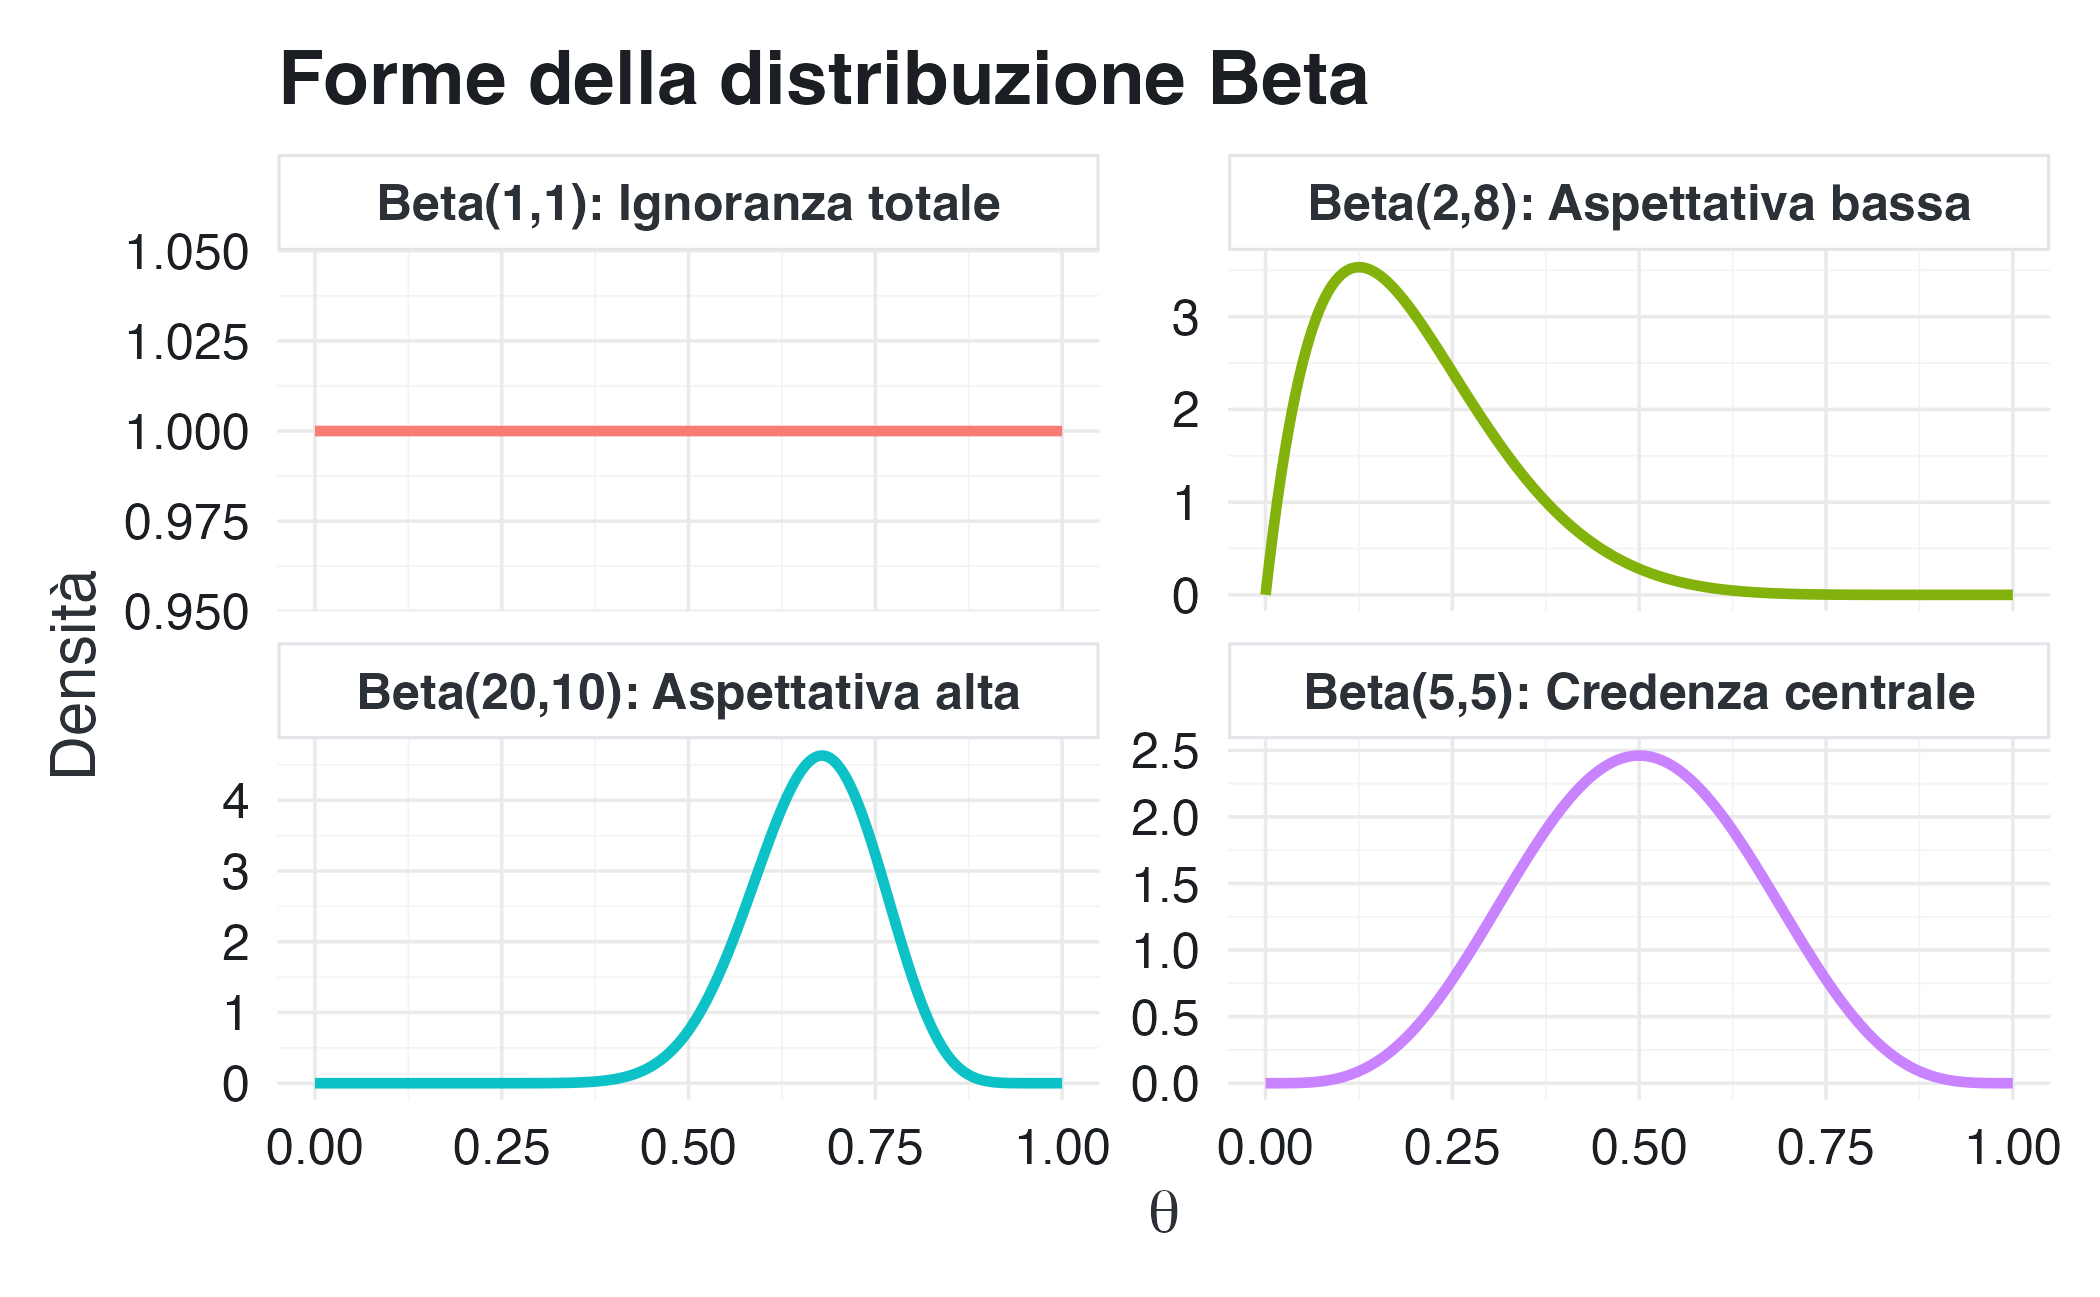
\includegraphics[width=0.85\linewidth,height=\textheight,keepaspectratio]{chapters/probability/03_equiprobability_combinatorics_bayesian_files/figure-pdf/unnamed-chunk-3-1.png}
\end{center}

\subsection{Due parametri, due
significati}\label{due-parametri-due-significati}

\begin{itemize}
\tightlist
\item
  \textbf{Posizione} (dove pensiamo che sia \(\theta\)):\\
  \[\mathbb{E}[\theta] = \frac{\alpha}{\alpha + \beta}\]
\item
  \textbf{Forza della convinzione} (quanto siamo sicuri):\\
  \(\alpha + \beta\) controlla la concentrazione. Valori alti →
  distribuzione stretta (sicurezza); valori bassi → distribuzione
  diffusa (incertezza).
\end{itemize}

\subsection{Beta(1,1): l'equiprobabilità
continua}\label{beta11-lequiprobabilituxe0-continua}

Beta(1,1) è semplicemente la \textbf{distribuzione uniforme} su
{[}0,1{]}: ogni valore è ugualmente plausibile. Rappresenta l'analogo
\emph{continuo} del principio di indifferenza:

\[
\text{Equiprobabilità discreta} \longleftrightarrow \text{Uniformità continua (Beta(1,1))}
\]

\subsection{Aggiornamento bayesiano: il modello
Beta-Binomiale}\label{aggiornamento-bayesiano-il-modello-beta-binomiale}

Se partiamo da \(\text{Beta}(\alpha, \beta)\) e osserviamo \(k\)
successi su \(n\) prove, la nuova credenza (posteriore) è:

\[
\theta \sim \text{Beta}(\alpha, \beta)
\;\xrightarrow{\text{osserviamo } k \text{ su } n}\;
\theta \mid k \sim \text{Beta}(\alpha + k, \beta + n - k).
\]

I successi osservati si ``aggiungono'' ad \(\alpha\), gli insuccessi a
\(\beta\). L'aggiornamento è intuitivo: la conoscenza precedente si
combina con i nuovi dati.

\begin{tcolorbox}[enhanced jigsaw, arc=.35mm, bottomrule=.15mm, bottomtitle=1mm, breakable, colback=white, colbacktitle=quarto-callout-note-color!10!white, colframe=quarto-callout-note-color-frame, coltitle=black, left=2mm, leftrule=.75mm, opacityback=0, opacitybacktitle=0.6, rightrule=.15mm, title=\textcolor{quarto-callout-note-color}{\faInfo}\hspace{0.5em}{Esempio: test a scelta multipla}, titlerule=0mm, toprule=.15mm, toptitle=1mm]

Uno studente risponde a 20 domande a scelta multipla (4 opzioni).
Adottiamo un prior Beta(1,3), che riflette l'ipotesi di risposte casuali
(media = 0.25). Se osserva 7 risposte corrette, la posterior diventa
Beta(8,16), con media \(8/24 \approx 0.33\).

\begin{Shaded}
\begin{Highlighting}[]
\NormalTok{prior }\OtherTok{\textless{}{-}} \FunctionTok{dbeta}\NormalTok{(theta, }\DecValTok{1}\NormalTok{, }\DecValTok{3}\NormalTok{)}
\NormalTok{posterior }\OtherTok{\textless{}{-}} \FunctionTok{dbeta}\NormalTok{(theta, }\DecValTok{8}\NormalTok{, }\DecValTok{16}\NormalTok{)}
\NormalTok{df }\OtherTok{\textless{}{-}} \FunctionTok{data.frame}\NormalTok{(}
  \AttributeTok{theta =} \FunctionTok{rep}\NormalTok{(theta, }\DecValTok{2}\NormalTok{),}
  \AttributeTok{Densita =} \FunctionTok{c}\NormalTok{(prior, posterior),}
  \AttributeTok{Tipo =} \FunctionTok{rep}\NormalTok{(}\FunctionTok{c}\NormalTok{(}\StringTok{"Prior Beta(1,3)"}\NormalTok{, }\StringTok{"Posterior Beta(8,16)"}\NormalTok{), }\AttributeTok{each =} \DecValTok{500}\NormalTok{)}
\NormalTok{)}
\FunctionTok{ggplot}\NormalTok{(df, }\FunctionTok{aes}\NormalTok{(}\AttributeTok{x =}\NormalTok{ theta, }\AttributeTok{y =}\NormalTok{ Densita, }\AttributeTok{color =}\NormalTok{ Tipo)) }\SpecialCharTok{+}
  \FunctionTok{geom\_line}\NormalTok{(}\AttributeTok{linewidth =} \FloatTok{1.3}\NormalTok{) }\SpecialCharTok{+}
  \FunctionTok{geom\_vline}\NormalTok{(}\AttributeTok{xintercept =} \FunctionTok{c}\NormalTok{(}\FloatTok{0.25}\NormalTok{, }\FloatTok{0.33}\NormalTok{), }\AttributeTok{linetype =} \StringTok{"dashed"}\NormalTok{, }\AttributeTok{alpha =} \FloatTok{0.5}\NormalTok{) }\SpecialCharTok{+}
  \FunctionTok{labs}\NormalTok{(}\AttributeTok{title =} \StringTok{"Aggiornamento bayesiano: prima e dopo 20 risposte"}\NormalTok{,}
       \AttributeTok{x =} \FunctionTok{expression}\NormalTok{(theta }\SpecialCharTok{\textasciitilde{}} \StringTok{"(probabilità di risposta corretta)"}\NormalTok{),}
       \AttributeTok{y =} \StringTok{"Densità"}\NormalTok{)}
\end{Highlighting}
\end{Shaded}

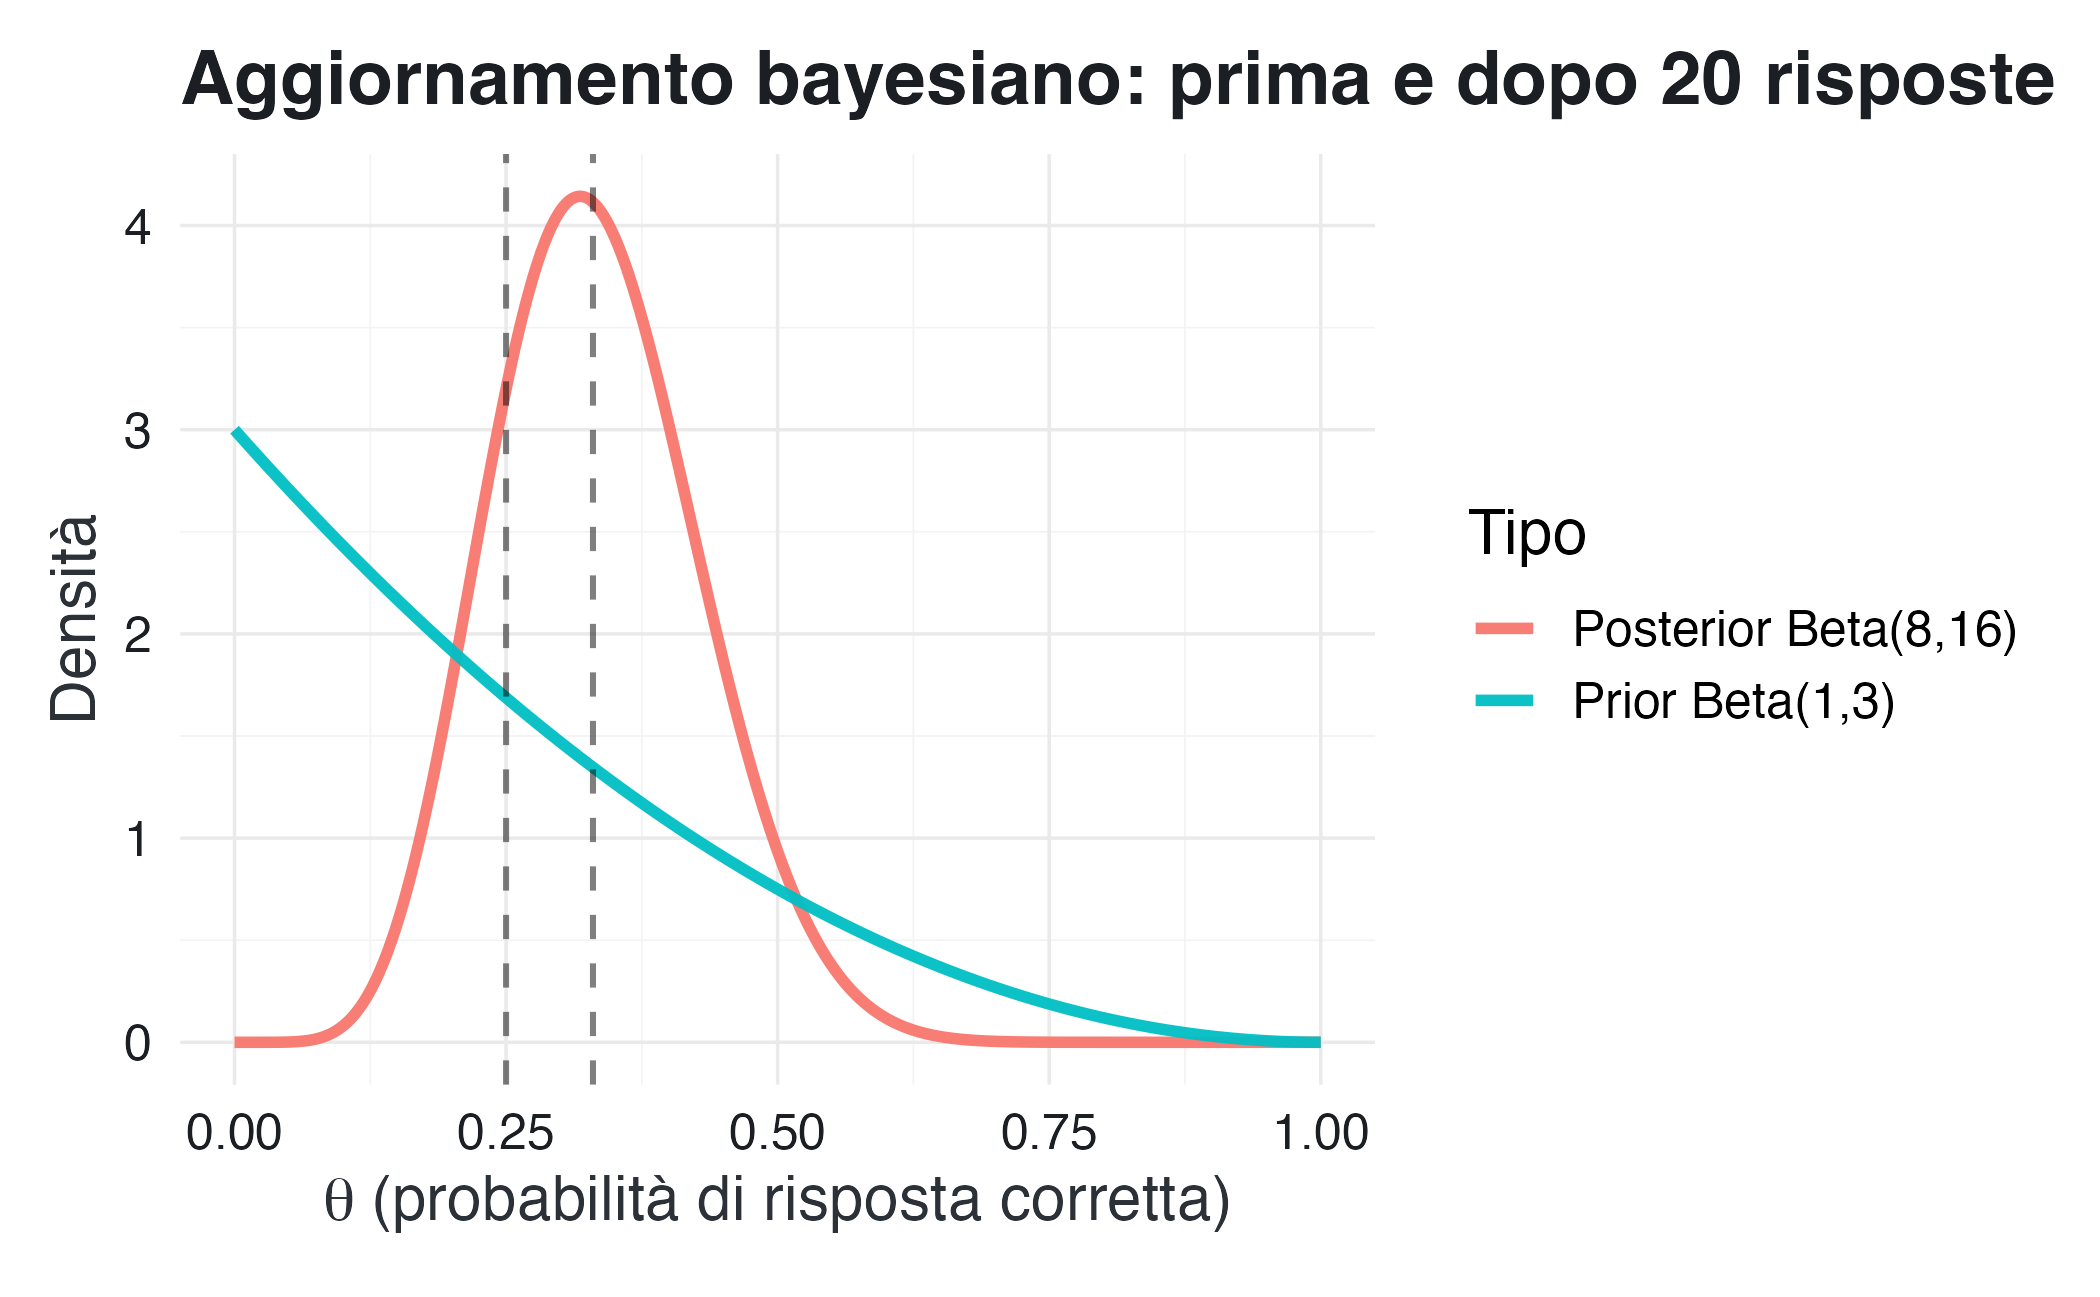
\includegraphics[width=0.85\linewidth,height=\textheight,keepaspectratio]{chapters/probability/03_equiprobability_combinatorics_bayesian_files/figure-pdf/unnamed-chunk-4-1.png}

\textbf{Intervallo di credibilità 95\%}:

\begin{Shaded}
\begin{Highlighting}[]
\NormalTok{alpha\_post }\OtherTok{\textless{}{-}} \DecValTok{8}\NormalTok{; beta\_post }\OtherTok{\textless{}{-}} \DecValTok{16}
\NormalTok{ci }\OtherTok{\textless{}{-}} \FunctionTok{qbeta}\NormalTok{(}\FunctionTok{c}\NormalTok{(}\FloatTok{0.025}\NormalTok{, }\FloatTok{0.975}\NormalTok{), alpha\_post, beta\_post)}
\FunctionTok{cat}\NormalTok{(}\StringTok{"Media posteriore:"}\NormalTok{, }\FunctionTok{round}\NormalTok{(alpha\_post}\SpecialCharTok{/}\NormalTok{(alpha\_post }\SpecialCharTok{+}\NormalTok{ beta\_post), }\DecValTok{3}\NormalTok{), }\StringTok{"}\SpecialCharTok{\textbackslash{}n}\StringTok{"}\NormalTok{)}
\CommentTok{\#\textgreater{} Media posteriore: 0.333}
\FunctionTok{cat}\NormalTok{(}\StringTok{"Intervallo 95\%: ["}\NormalTok{, }\FunctionTok{round}\NormalTok{(ci[}\DecValTok{1}\NormalTok{], }\DecValTok{2}\NormalTok{), }\StringTok{","}\NormalTok{, }\FunctionTok{round}\NormalTok{(ci[}\DecValTok{2}\NormalTok{], }\DecValTok{2}\NormalTok{), }\StringTok{"]"}\NormalTok{)}
\CommentTok{\#\textgreater{} Intervallo 95\%: [ 0.16 , 0.53 ]}
\end{Highlighting}
\end{Shaded}

L'intervallo {[}0.18, 0.52{]} esprime l'incertezza residua: siamo
ragionevolmente sicuri che la probabilità vera si trovi lì, ma
l'intervallo è ancora piuttosto ampio.

\end{tcolorbox}

\subsection{Aggiornamento sequenziale: la conoscenza si
accumula}\label{aggiornamento-sequenziale-la-conoscenza-si-accumula}

Una conseguenza pratica importante è che l'aggiornamento può avvenire
\textbf{man mano che si osservano nuovi dati}, senza ricalcolare tutto
da capo.

\begin{Shaded}
\begin{Highlighting}[]
\FunctionTok{set.seed}\NormalTok{(}\DecValTok{42}\NormalTok{)}
\NormalTok{theta\_vero }\OtherTok{\textless{}{-}} \FloatTok{0.4}
\NormalTok{n\_domande }\OtherTok{\textless{}{-}} \DecValTok{20}
\NormalTok{risposte }\OtherTok{\textless{}{-}} \FunctionTok{rbinom}\NormalTok{(n\_domande, }\DecValTok{1}\NormalTok{, theta\_vero)}
\NormalTok{alpha }\OtherTok{\textless{}{-}} \DecValTok{1}\NormalTok{; beta }\OtherTok{\textless{}{-}} \DecValTok{3}
\NormalTok{theta\_grid }\OtherTok{\textless{}{-}} \FunctionTok{seq}\NormalTok{(}\DecValTok{0}\NormalTok{, }\DecValTok{1}\NormalTok{, }\AttributeTok{length.out =} \DecValTok{200}\NormalTok{)}
\NormalTok{df\_evol }\OtherTok{\textless{}{-}} \FunctionTok{data.frame}\NormalTok{()}
\ControlFlowTok{for}\NormalTok{(i }\ControlFlowTok{in} \FunctionTok{c}\NormalTok{(}\DecValTok{0}\NormalTok{, }\DecValTok{5}\NormalTok{, }\DecValTok{10}\NormalTok{, }\DecValTok{20}\NormalTok{)) \{}
  \ControlFlowTok{if}\NormalTok{(i }\SpecialCharTok{==} \DecValTok{0}\NormalTok{) \{}
\NormalTok{    dens }\OtherTok{\textless{}{-}} \FunctionTok{dbeta}\NormalTok{(theta\_grid, alpha, beta)}
\NormalTok{    label }\OtherTok{\textless{}{-}} \StringTok{"Prior (n=0)"}
\NormalTok{  \} }\ControlFlowTok{else}\NormalTok{ \{}
\NormalTok{    a }\OtherTok{\textless{}{-}} \DecValTok{1} \SpecialCharTok{+} \FunctionTok{sum}\NormalTok{(risposte[}\DecValTok{1}\SpecialCharTok{:}\NormalTok{i])}
\NormalTok{    b }\OtherTok{\textless{}{-}} \DecValTok{3} \SpecialCharTok{+}\NormalTok{ i }\SpecialCharTok{{-}} \FunctionTok{sum}\NormalTok{(risposte[}\DecValTok{1}\SpecialCharTok{:}\NormalTok{i])}
\NormalTok{    dens }\OtherTok{\textless{}{-}} \FunctionTok{dbeta}\NormalTok{(theta\_grid, a, b)}
\NormalTok{    label }\OtherTok{\textless{}{-}} \FunctionTok{paste0}\NormalTok{(}\StringTok{"n = "}\NormalTok{, i)}
\NormalTok{  \}}
\NormalTok{  df\_evol }\OtherTok{\textless{}{-}} \FunctionTok{rbind}\NormalTok{(df\_evol, }\FunctionTok{data.frame}\NormalTok{(}
    \AttributeTok{theta =}\NormalTok{ theta\_grid, }\AttributeTok{Densita =}\NormalTok{ dens, }\AttributeTok{n =}\NormalTok{ label}
\NormalTok{  ))}
\NormalTok{\}}
\FunctionTok{ggplot}\NormalTok{(df\_evol, }\FunctionTok{aes}\NormalTok{(}\AttributeTok{x =}\NormalTok{ theta, }\AttributeTok{y =}\NormalTok{ Densita, }\AttributeTok{color =}\NormalTok{ n)) }\SpecialCharTok{+}
  \FunctionTok{geom\_line}\NormalTok{(}\AttributeTok{linewidth =} \FloatTok{1.2}\NormalTok{) }\SpecialCharTok{+}
  \FunctionTok{geom\_vline}\NormalTok{(}\AttributeTok{xintercept =}\NormalTok{ theta\_vero, }\AttributeTok{linetype =} \StringTok{"dashed"}\NormalTok{) }\SpecialCharTok{+}
  \FunctionTok{annotate}\NormalTok{(}\StringTok{"text"}\NormalTok{, }\AttributeTok{x =}\NormalTok{ theta\_vero }\SpecialCharTok{+} \FloatTok{0.05}\NormalTok{, }\AttributeTok{y =} \FunctionTok{max}\NormalTok{(df\_evol}\SpecialCharTok{$}\NormalTok{Densita) }\SpecialCharTok{*} \FloatTok{0.9}\NormalTok{,}
           \AttributeTok{label =} \FunctionTok{expression}\NormalTok{(theta}\SpecialCharTok{\textasciitilde{}}\StringTok{"vero"}\NormalTok{), }\AttributeTok{hjust =} \DecValTok{0}\NormalTok{) }\SpecialCharTok{+}
  \FunctionTok{labs}\NormalTok{(}\AttributeTok{title =} \StringTok{"Evoluzione delle credenze all\textquotesingle{}accumularsi dei dati"}\NormalTok{,}
       \AttributeTok{x =} \FunctionTok{expression}\NormalTok{(theta), }\AttributeTok{y =} \StringTok{"Densità"}\NormalTok{, }\AttributeTok{color =} \StringTok{"Osservazioni"}\NormalTok{)}
\end{Highlighting}
\end{Shaded}

\begin{center}
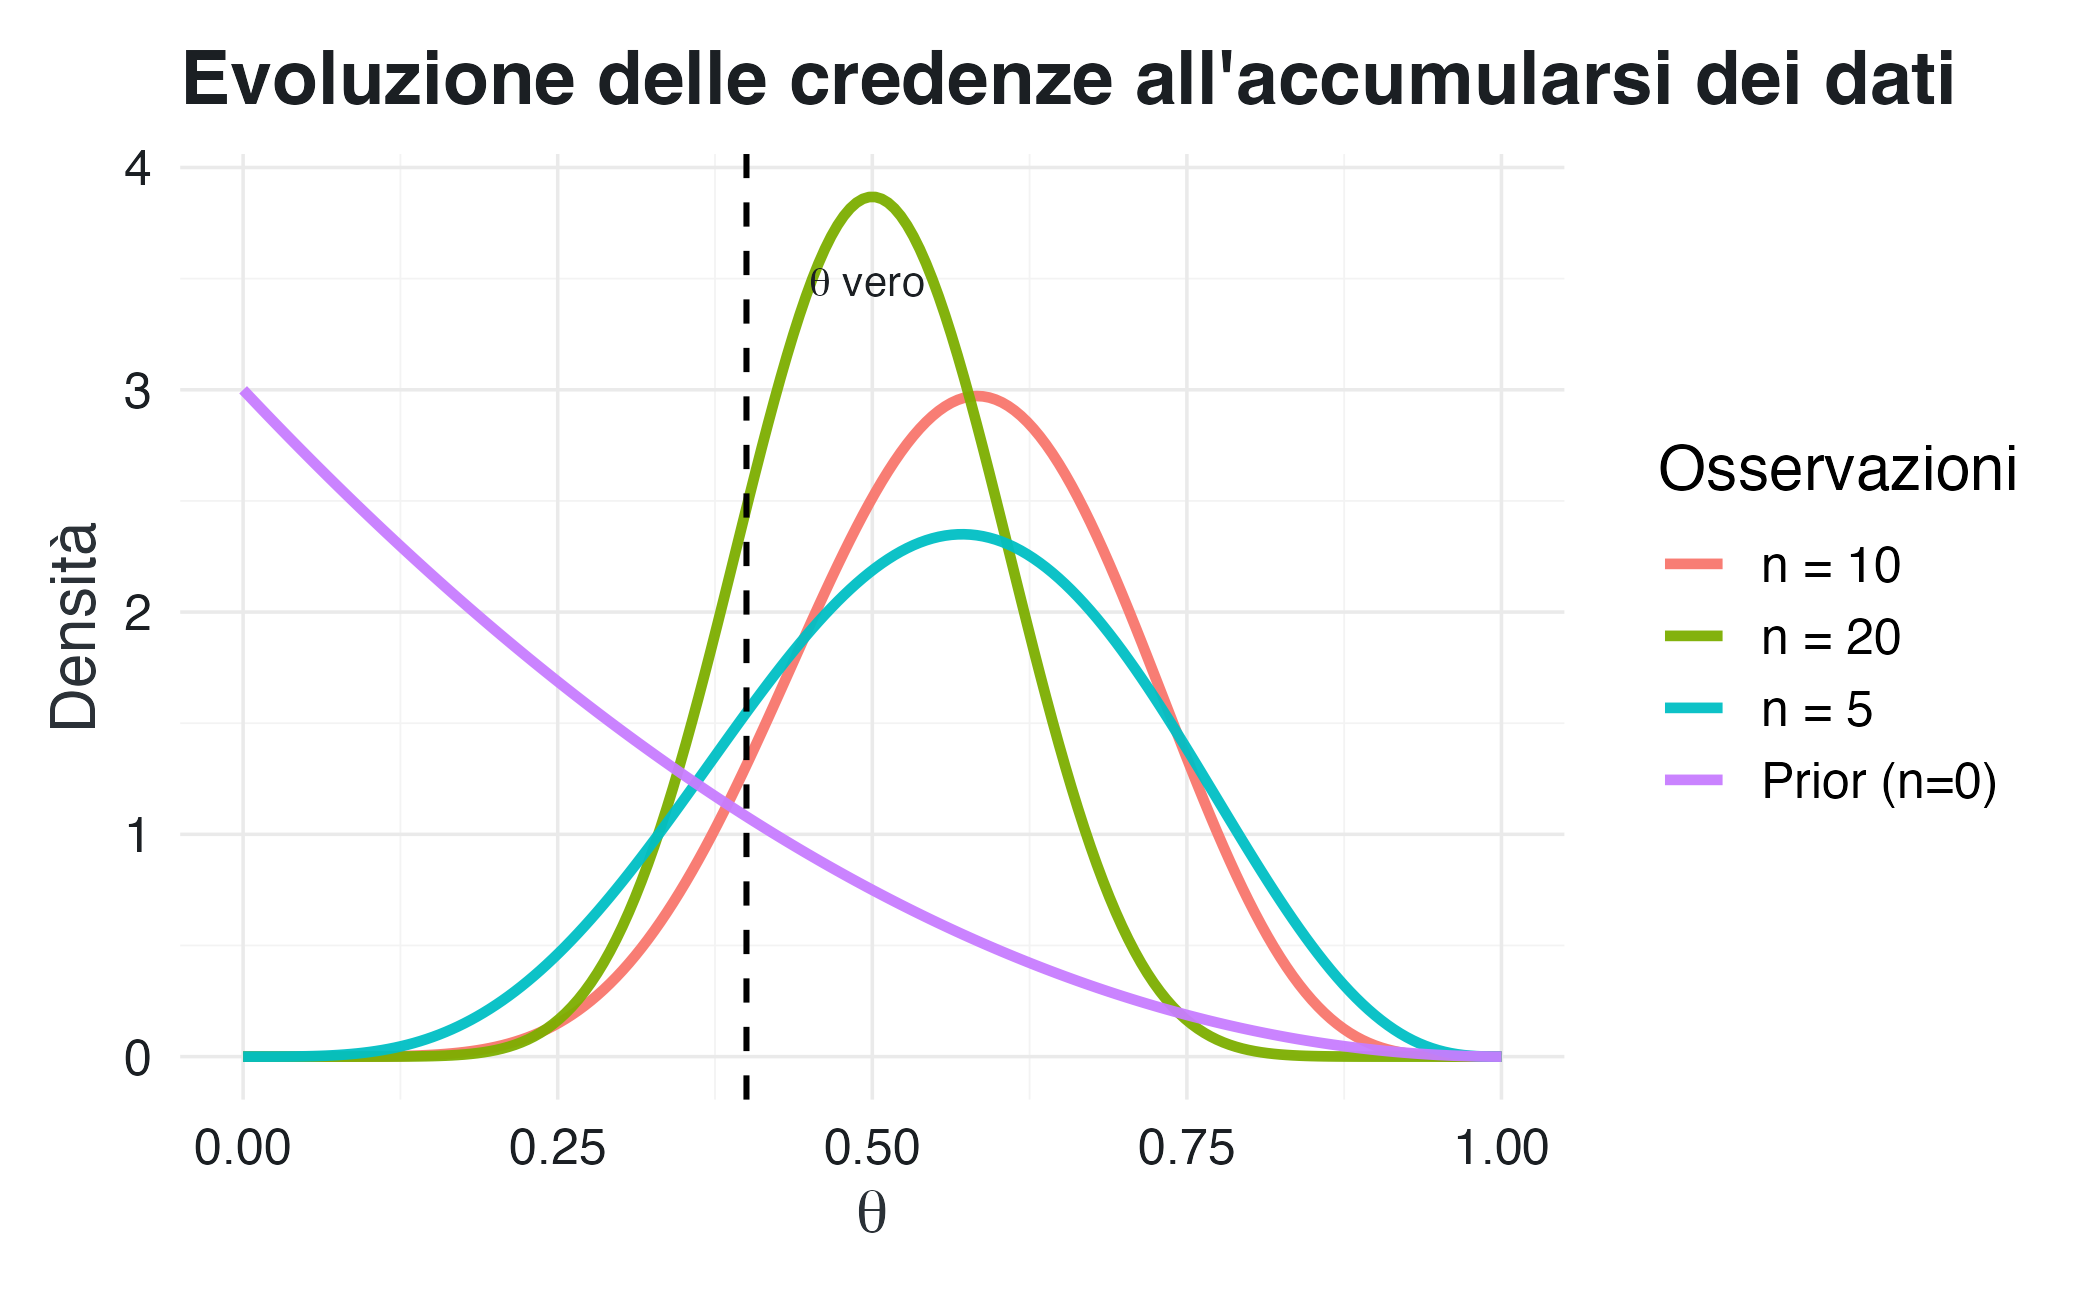
\includegraphics[width=0.85\linewidth,height=\textheight,keepaspectratio]{chapters/probability/03_equiprobability_combinatorics_bayesian_files/figure-pdf/unnamed-chunk-6-1.png}
\end{center}

La distribuzione si sposta gradualmente verso il valore vero
(\(\theta = 0.4\)) e si restringe, riflettendo una crescente certezza.

\section{Applicazioni psicologiche}\label{sec-applications-psychology}

Gli strumenti che abbiamo sviluppato trovano applicazione diretta in
contesti psicologici concreti.

\subsection{Item Response Theory (IRT)}\label{item-response-theory-irt}

La \textbf{teoria della risposta agli item} formalizza ciò che ogni
insegnante sa intuitivamente: la probabilità di rispondere correttamente
a una domanda dipende sia dallo studente che dalla domanda. Il modello
base è:

\[
P(\text{corretto} \mid \theta, b) = \frac{1}{1 + e^{-(\theta - b)}},
\]

dove \(\theta\) è l'abilità dello studente e \(b\) la difficoltà
dell'item. Questa formulazione \textbf{rifiuta esplicitamente}
l'equiprobabilità, riconoscendo che gli item hanno difficoltà diverse e
che la probabilità di risposta corretta varia sistematicamente.

\subsection{Bias di risposta nei
questionari}\label{bias-di-risposta-nei-questionari}

Le risposte ai questionari sono influenzate da fenomeni sistematici come
l'\textbf{acquiescenza} (tendenza a rispondere ``sì''), la
\textbf{desiderabilità sociale} o gli \textbf{effetti di posizione}.
Questi bias significano che le opzioni di risposta non sono
equiprobabili. Un modello adeguato deve esplicitare queste tendenze,
distinguendo la variabilità dovuta al costrutto misurato da quella
dovuta allo stile di risposta.

\subsection{Efficacia degli
interventi}\label{efficacia-degli-interventi}

Quando si valuta l'efficacia di un trattamento, l'equiprobabilità è
particolarmente inappropriata. Non tutti i pazienti rispondono allo
stesso modo. L'approccio bayesiano permette di:

\begin{enumerate}
\def\labelenumi{\arabic{enumi}.}
\tightlist
\item
  iniziare con prior informativi basati su studi precedenti;
\item
  aggiornare progressivamente man mano che i dati si accumulano;
\item
  rappresentare esplicitamente la variabilità interindividuale;
\item
  quantificare l'incertezza in modo interpretabile.
\end{enumerate}

Questo approccio produce stime che riconoscono la complessità del
fenomeno, invece di nasconderla sotto l'ipotesi di uniformità.

\section*{Riflessioni conclusive}\label{riflessioni-conclusive-2}

\markright{Riflessioni conclusive}

Siamo partiti da una domanda apparentemente ingenua --- ``Quando
possiamo dire che gli esiti sono `ugualmente probabili'?'' --- e abbiamo
scoperto che la risposta ci porta al cuore dell'epistemologia della
probabilità.

L'equiprobabilità non è un fatto del mondo. È una \textbf{scelta
inferenziale} che riflette uno stato particolare di conoscenza: quello
in cui non abbiamo ragioni per distinguere tra le varie possibilità. La
formula ``casi favorevoli su casi possibili'' è una conseguenza di
questa assunzione, non una legge universale.

Nella ricerca psicologica, l'equiprobabilità è quasi sempre violata.
Questa variabilità non è un fastidio da eliminare: è spesso la
\emph{sostanza} stessa di ciò che studiamo. La distribuzione Beta ci
offre un primo strumento per andare oltre, consentendo di rappresentare
credenze con forme e intensità diverse.

Nel prossimo capitolo vedremo come la \textbf{probabilità condizionata}
e il \textbf{teorema di Bayes} formalizzino il processo di apprendimento
dall'esperienza --- non solo quando partiamo dall'equiprobabilità, ma
anche quando disponiamo di informazioni strutturate.

\section*{Punti chiave da ricordare}\label{punti-chiave-da-ricordare-2}

\markright{Punti chiave da ricordare}

\begin{tcolorbox}[enhanced jigsaw, arc=.35mm, bottomrule=.15mm, bottomtitle=1mm, breakable, colback=white, colbacktitle=quarto-callout-important-color!10!white, colframe=quarto-callout-important-color-frame, coltitle=black, left=2mm, leftrule=.75mm, opacityback=0, opacitybacktitle=0.6, rightrule=.15mm, title=\textcolor{quarto-callout-important-color}{\faExclamation}\hspace{0.5em}{Importante}, titlerule=0mm, toprule=.15mm, toptitle=1mm]

\begin{enumerate}
\def\labelenumi{\arabic{enumi}.}
\item
  \textbf{Principio di indifferenza}: l'equiprobabilità riflette
  simmetria epistemica, non una proprietà fisica. Assegniamo
  \(P(\omega_i) = 1/n\) solo quando non abbiamo ragioni per preferire un
  esito.
\item
  \textbf{Formula classica come caso speciale}: \(P(A) = |A|/|\Omega|\)
  è una \emph{conseguenza} degli assiomi quando vale l'equiprobabilità,
  non una definizione universale.
\item
  \textbf{Tecniche combinatorie}:

  \begin{itemize}
  \tightlist
  \item
    Permutazioni: \(n!\) (ordine conta, tutti gli elementi)
  \item
    Disposizioni: \(n!/(n-k)!\) (ordine conta, \(k\) elementi)
  \item
    Combinazioni: \(\binom{n}{k}\) (ordine non conta)
  \end{itemize}
\item
  \textbf{Distribuzione Beta}:

  \begin{itemize}
  \tightlist
  \item
    Beta(1,1) = massima ignoranza (equiprobabilità continua).
  \item
    Aggiornamento:
    \(\text{Beta}(\alpha, \beta) \to \text{Beta}(\alpha+k, \beta+n-k)\).
  \end{itemize}
\item
  \textbf{Limiti dell'equiprobabilità in psicologia}: IRT, bias di
  risposta e variabilità interindividuale richiedono modelli flessibili
  che vadano oltre l'assunzione di uniformità.
\end{enumerate}

\end{tcolorbox}

\begin{tcolorbox}[enhanced jigsaw, arc=.35mm, bottomrule=.15mm, bottomtitle=1mm, breakable, colback=white, colbacktitle=quarto-callout-note-color!10!white, colframe=quarto-callout-note-color-frame, coltitle=black, left=2mm, leftrule=.75mm, opacityback=0, opacitybacktitle=0.6, rightrule=.15mm, title=\textcolor{quarto-callout-note-color}{\faInfo}\hspace{0.5em}{Informazioni sull'ambiente di sviluppo}, titlerule=0mm, toprule=.15mm, toptitle=1mm]

\begin{Shaded}
\begin{Highlighting}[]
\FunctionTok{sessionInfo}\NormalTok{()}
\CommentTok{\#\textgreater{} R version 4.6.1 (2026{-}06{-}24)}
\CommentTok{\#\textgreater{} Platform: aarch64{-}apple{-}darwin23}
\CommentTok{\#\textgreater{} Running under: macOS Tahoe 26.5.2}
\CommentTok{\#\textgreater{} }
\CommentTok{\#\textgreater{} Matrix products: default}
\CommentTok{\#\textgreater{} BLAS:   /Library/Frameworks/R.framework/Versions/4.6/Resources/lib/libRblas.0.dylib }
\CommentTok{\#\textgreater{} LAPACK: /Library/Frameworks/R.framework/Versions/4.6/Resources/lib/libRlapack.dylib;  LAPACK version 3.12.1}
\CommentTok{\#\textgreater{} }
\CommentTok{\#\textgreater{} locale:}
\CommentTok{\#\textgreater{} [1] C.UTF{-}8/UTF{-}8/C.UTF{-}8/C/C.UTF{-}8/C.UTF{-}8}
\CommentTok{\#\textgreater{} }
\CommentTok{\#\textgreater{} time zone: Europe/Rome}
\CommentTok{\#\textgreater{} tzcode source: internal}
\CommentTok{\#\textgreater{} }
\CommentTok{\#\textgreater{} attached base packages:}
\CommentTok{\#\textgreater{} [1] stats     graphics  grDevices utils     datasets  methods   base     }
\CommentTok{\#\textgreater{} }
\CommentTok{\#\textgreater{} other attached packages:}
\CommentTok{\#\textgreater{}  [1] gtools\_3.9.5          combinat\_0.0{-}8        ragg\_1.5.2           }
\CommentTok{\#\textgreater{}  [4] tinytable\_0.17.0      withr\_3.0.3           systemfonts\_1.3.2    }
\CommentTok{\#\textgreater{}  [7] patchwork\_1.3.2       ggdist\_3.3.3          tidybayes\_3.0.7      }
\CommentTok{\#\textgreater{} [10] bayesplot\_1.15.0      ggplot2\_4.0.3         reliabilitydiag\_0.2.1}
\CommentTok{\#\textgreater{} [13] priorsense\_1.2.0      posterior\_1.7.0       loo\_2.10.0           }
\CommentTok{\#\textgreater{} [16] rstan\_2.32.7          StanHeaders\_2.32.10   brms\_2.23.0          }
\CommentTok{\#\textgreater{} [19] Rcpp\_1.1.2            sessioninfo\_1.2.4     conflicted\_1.2.0     }
\CommentTok{\#\textgreater{} [22] janitor\_2.2.1         matrixStats\_1.5.0     modelr\_0.1.11        }
\CommentTok{\#\textgreater{} [25] tibble\_3.3.1          dplyr\_1.2.1           tidyr\_1.3.2          }
\CommentTok{\#\textgreater{} [28] rio\_1.3.0             here\_1.0.2           }
\CommentTok{\#\textgreater{} }
\CommentTok{\#\textgreater{} loaded via a namespace (and not attached):}
\CommentTok{\#\textgreater{}  [1] svUnit\_1.0.8          tidyselect\_1.2.1      farver\_2.1.2         }
\CommentTok{\#\textgreater{}  [4] S7\_0.2.2              fastmap\_1.2.0         tensorA\_0.36.2.1     }
\CommentTok{\#\textgreater{}  [7] pacman\_0.5.1          digest\_0.6.39         timechange\_0.4.0     }
\CommentTok{\#\textgreater{} [10] estimability\_2.0.0    lifecycle\_1.0.5       magrittr\_2.0.5       }
\CommentTok{\#\textgreater{} [13] compiler\_4.6.1        rlang\_1.3.0           tools\_4.6.1          }
\CommentTok{\#\textgreater{} [16] yaml\_2.3.12           knitr\_1.51            labeling\_0.4.3       }
\CommentTok{\#\textgreater{} [19] bridgesampling\_1.2{-}1  pkgbuild\_1.4.8        curl\_7.1.0           }
\CommentTok{\#\textgreater{} [22] RColorBrewer\_1.1{-}3    abind\_1.4{-}8           purrr\_1.2.2          }
\CommentTok{\#\textgreater{} [25] grid\_4.6.1            stats4\_4.6.1          xtable\_1.8{-}8         }
\CommentTok{\#\textgreater{} [28] inline\_0.3.21         emmeans\_2.0.3         scales\_1.4.0         }
\CommentTok{\#\textgreater{} [31] cli\_3.6.6             mvtnorm\_1.4{-}1         rmarkdown\_2.31       }
\CommentTok{\#\textgreater{} [34] generics\_0.1.4        otel\_0.2.0            RcppParallel\_5.1.11{-}2}
\CommentTok{\#\textgreater{} [37] cachem\_1.1.0          stringr\_1.6.0         parallel\_4.6.1       }
\CommentTok{\#\textgreater{} [40] vctrs\_0.7.3           V8\_8.2.0              Matrix\_1.7{-}5         }
\CommentTok{\#\textgreater{} [43] jsonlite\_2.0.0        arrayhelpers\_1.1{-}1    glue\_1.8.1           }
\CommentTok{\#\textgreater{} [46] codetools\_0.2{-}20      distributional\_0.8.1  lubridate\_1.9.5      }
\CommentTok{\#\textgreater{} [49] stringi\_1.8.7         gtable\_0.3.6          QuickJSR\_1.10.0      }
\CommentTok{\#\textgreater{} [52] pillar\_1.11.1         htmltools\_0.5.9       Brobdingnag\_1.2{-}9    }
\CommentTok{\#\textgreater{} [55] R6\_2.6.1              textshaping\_1.0.5     rprojroot\_2.1.1      }
\CommentTok{\#\textgreater{} [58] evaluate\_1.0.5        lattice\_0.22{-}9        backports\_1.5.1      }
\CommentTok{\#\textgreater{} [61] memoise\_2.0.1         broom\_1.0.13          snakecase\_0.11.1     }
\CommentTok{\#\textgreater{} [64] rstantools\_2.6.0      coda\_0.19{-}4.1         gridExtra\_2.3.1      }
\CommentTok{\#\textgreater{} [67] nlme\_3.1{-}169          checkmate\_2.3.4       xfun\_0.60            }
\CommentTok{\#\textgreater{} [70] pkgconfig\_2.0.3}
\end{Highlighting}
\end{Shaded}

\end{tcolorbox}

\chapter{Probabilità condizionata come
aggiornamento}\label{sec-prob-conditional-prob}

\section*{Introduzione}\label{introduzione-3}

\markright{Introduzione}

Immaginate di essere uno psicologo clinico che ha appena ricevuto
l'esito positivo di un test diagnostico per un paziente. Prima della
somministrazione, avevate formulato una stima della probabilità di
depressione. Ora il referto è sul tavolo. Cosa è cambiato?

\textbf{Tutto e niente.} I fatti oggettivi restano immutati: il paziente
era depresso, o non lo era, già prima che il test venisse eseguito. Ciò
che è radicalmente mutato è il vostro stato di conoscenza. Avete
acquisito un'informazione nuova che deve essere incorporata in modo
coerente, ristrutturando sistematicamente la valutazione iniziale.

Questo processo dinamico di revisione razionale delle credenze alla luce
dell'evidenza empirica costituisce l'essenza stessa del pensiero
bayesiano. Lo strumento formale che lo incarna è la \textbf{probabilità
condizionata}, il ponte matematico che collega le conoscenze precedenti
a quelle successive all'osservazione.

In questo capitolo esploreremo la probabilità condizionata da diverse
angolazioni:

\begin{itemize}
\tightlist
\item
  come \textbf{meccanismo di aggiornamento} epistemico;
\item
  come \textbf{fondamento dell'indipendenza};
\item
  come \textbf{strumento per costruire modelli complessi};
\item
  come \textbf{protezione dagli errori} di aggregazione.
\end{itemize}

Questi concetti preparano direttamente il terreno per il teorema di
Bayes che, nel prossimo capitolo, emergerà come la regola per
``invertire'' le probabilità condizionate.

\begin{tcolorbox}[enhanced jigsaw, arc=.35mm, bottomrule=.15mm, bottomtitle=1mm, breakable, colback=white, colbacktitle=quarto-callout-tip-color!10!white, colframe=quarto-callout-tip-color-frame, coltitle=black, left=2mm, leftrule=.75mm, opacityback=0, opacitybacktitle=0.6, rightrule=.15mm, title=\textcolor{quarto-callout-tip-color}{\faLightbulb}\hspace{0.5em}{Prerequisiti}, titlerule=0mm, toprule=.15mm, toptitle=1mm]

Per seguire questo capitolo è necessario aver letto:

\begin{itemize}
\tightlist
\item
  Capitolo~\ref{sec-prob-interpretation}
\item
  Capitolo~\ref{sec-prob-axioms-coherence}
\item
  Capitolo~\ref{sec-equiprobability-combinatorics}
\end{itemize}

Conoscenze matematiche richieste:

\begin{itemize}
\tightlist
\item
  Appendice~\ref{sec-apx-sets} - per operazioni su eventi (intersezione,
  unione);
\item
  Appendice~\ref{sec-apx-sums} - per la legge della probabilità totale.
\end{itemize}

Competenze pratiche:

\begin{itemize}
\tightlist
\item
  Familiarità con tabelle congiunte e rappresentazioni 2×2;
\item
  Nozioni base di R per eseguire le simulazioni presentate.
\end{itemize}

\end{tcolorbox}

\begin{tcolorbox}[enhanced jigsaw, arc=.35mm, bottomrule=.15mm, bottomtitle=1mm, breakable, colback=white, colbacktitle=quarto-callout-caution-color!10!white, colframe=quarto-callout-caution-color-frame, coltitle=black, left=2mm, leftrule=.75mm, opacityback=0, opacitybacktitle=0.6, rightrule=.15mm, title=\textcolor{quarto-callout-caution-color}{\faFire}\hspace{0.5em}{Preparazione del Notebook}, titlerule=0mm, toprule=.15mm, toptitle=1mm]

\begin{Shaded}
\begin{Highlighting}[]
\NormalTok{here}\SpecialCharTok{::}\FunctionTok{here}\NormalTok{(}\StringTok{"code"}\NormalTok{, }\StringTok{"\_common.R"}\NormalTok{) }\SpecialCharTok{|\textgreater{}} 
  \FunctionTok{source}\NormalTok{()}

\CommentTok{\# Load packages}
\ControlFlowTok{if}\NormalTok{ (}\SpecialCharTok{!}\FunctionTok{requireNamespace}\NormalTok{(}\StringTok{"pacman"}\NormalTok{)) }\FunctionTok{install.packages}\NormalTok{(}\StringTok{"pacman"}\NormalTok{)}
\NormalTok{pacman}\SpecialCharTok{::}\FunctionTok{p\_load}\NormalTok{(patchwork, ggforce)}
\CommentTok{\# Riapplica il tema per sicurezza}
\FunctionTok{apply\_visual\_theme}\NormalTok{()}
\end{Highlighting}
\end{Shaded}

\end{tcolorbox}

\section{Definizione e interpretazione
epistemica}\label{sec-conditional-definition}

Partiamo da una credenza iniziale in un evento \(A\). Poi apprendiamo
che si è verificato un altro evento \(B\). Come dovrebbe cambiare la
nostra credenza in \(A\)?

La risposta intuitiva è che dovremmo considerare solo le situazioni in
cui \(B\) è vero e vedere quanto spesso \(A\) è vero \emph{in quelle
situazioni}. La formula seguente traduce esattamente questa intuizione
in linguaggio matematico.

\begin{definition}[Probabilità
condizionata]\protect\hypertarget{def-conditional-probability}{}\label{def-conditional-probability}

Se \(P(B) > 0\), la \emph{probabilità condizionata} di \(A\) dato \(B\)
è definita come:

\begin{equation}\protect\phantomsection\label{eq-prob-cond-def}{
P(A \mid B) = \frac{P(A \cap B)}{P(B)}.
}\end{equation}

\textbf{Interpretazione epistemica}: \(P(A \mid B)\) quantifica il
nostro grado di credenza in \(A\) dopo aver appreso che \(B\) è vero,
tenendo conto del fatto che ora lo spazio delle possibilità si è
ristretto a quelle compatibili con \(B\).

\end{definition}

\subsection{Il meccanismo
dell'aggiornamento}\label{il-meccanismo-dellaggiornamento}

Apprendere che \(B\) è vero innesca un processo in due fasi:

\textbf{1. Riduzione epistemica} --- Lo spazio delle possibilità
\(\Omega\) viene ristretto al solo sottoinsieme \(B\). Tutte le
configurazioni in cui \(B\) è falso vengono eliminate, non perché siano
diventate ``impossibili'' in senso metafisico, ma perché sono diventate
\emph{irrilevanti} per il nostro ragionamento.

\textbf{2. Rinormalizzazione} --- Le probabilità delle configurazioni
rimanenti (quelle in cui \(B\) è vero) vengono riscalate in modo che
tornino a sommare a 1. Il fattore di scala è esattamente \(1/P(B)\).

Questo procedimento garantisce \textbf{coerenza}: se avessimo modellato
fin dall'inizio un mondo in cui \(B\) è l'unica possibilità, avremmo
ottenuto esattamente le stesse probabilità relative.

\subsection{Un'analogia: lo zoom
fotografico}\label{unanalogia-lo-zoom-fotografico}

Pensate alla distribuzione di probabilità congiunta come a una
fotografia. La probabilità condizionata è come fare uno \emph{zoom} su
una porzione dell'immagine (la regione \(B\)):

\begin{itemize}
\tightlist
\item
  perdiamo di vista tutto ciò che sta fuori dalla regione (riduzione);
\item
  i dettagli della regione riempiono ora tutto lo schermo
  (rinormalizzazione);
\item
  i rapporti tra gli elementi \emph{all'interno} della regione rimangono
  invariati.
\end{itemize}

\begin{center}
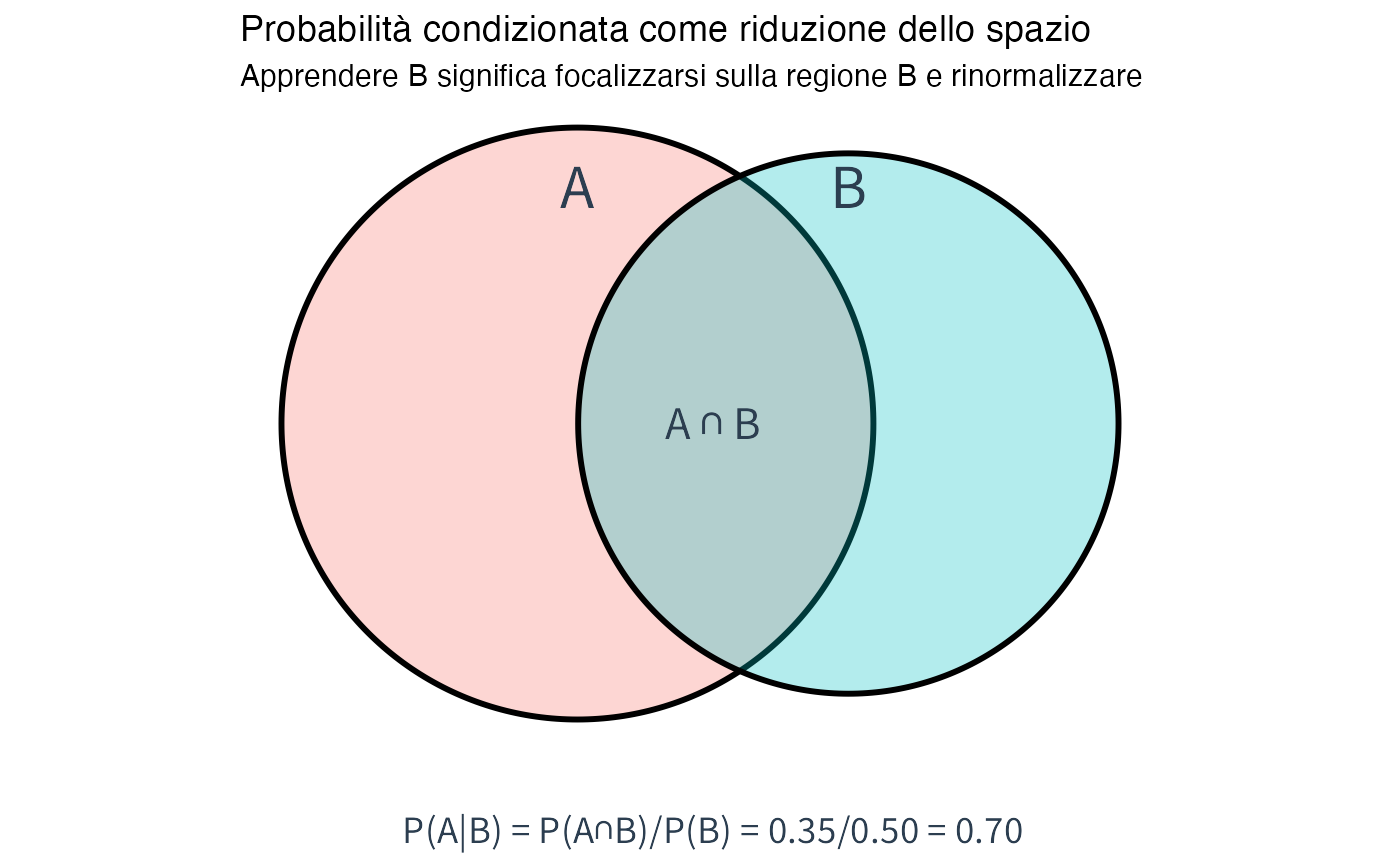
\includegraphics[width=0.85\linewidth,height=\textheight,keepaspectratio]{chapters/probability/04_conditional_prob_bayesian_files/figure-pdf/unnamed-chunk-2-1.png}
\end{center}

\subsection{Ogni probabilità è sempre
condizionata}\label{ogni-probabilituxe0-uxe8-sempre-condizionata}

C'è un punto filosofico importante da cogliere: dal punto di vista
bayesiano, \textbf{ogni probabilità è sempre condizionata}, anche quando
non lo scriviamo esplicitamente.

Quando diciamo ``\(P(A) = 0.3\)'', in realtà intendiamo
``\(P(A \mid \mathcal{I}) = 0.3\)'', dove \(\mathcal{I}\) rappresenta
tutto ciò che sappiamo: dati precedenti, teoria, contesto e assunzioni.
Non esistono probabilità assolute e prive di contesto.

Ciò significa che la notazione \(P(A)\) è un'abbreviazione comoda, non
una descrizione di una proprietà intrinseca del mondo.

\section{Proprietà della probabilità
condizionata}\label{sec-conditional-properties}

Un risultato importante è che le probabilità condizionate soddisfano
tutti gli assiomi della probabilità. In altre parole,
\(P(\cdot \mid B)\) è essa stessa una funzione di probabilità legittima.

\begin{theorem}[Proprietà della
condizionata]\protect\hypertarget{thm-conditional-properties}{}\label{thm-conditional-properties}

Fissato un evento \(B\) con \(P(B) > 0\), la funzione
\(P(\cdot \mid B)\) soddisfa:

\begin{enumerate}
\def\labelenumi{\arabic{enumi}.}
\item
  \textbf{Non-negatività}: \(P(A \mid B) \geq 0\) per ogni evento \(A\).
\item
  \textbf{Normalizzazione}: \(P(B \mid B) = 1\) (certezza di \(B\) dato
  \(B\)).
\item
  \textbf{Additività}: se \(A_1, A_2\) sono disgiunti,
  \[P(A_1 \cup A_2 \mid B) = P(A_1 \mid B) + P(A_2 \mid B).\]
\item
  \textbf{Complemento}: \(P(A^c \mid B) = 1 - P(A \mid B).\)
\item
  \textbf{Regola della catena}:
  \[P(A \cap B \mid C) = P(A \mid B \cap C) \cdot P(B \mid C).\]
\end{enumerate}

\end{theorem}

\textbf{Interpretazione epistemica}: queste proprietà ci dicono che il
ragionamento in condizioni di informazione parziale segue le stesse
regole del ragionamento in condizioni di informazione completa. Non
esistono ``leggi speciali'' per il condizionamento.

\begin{tcolorbox}[enhanced jigsaw, arc=.35mm, bottomrule=.15mm, bottomtitle=1mm, breakable, colback=white, colbacktitle=quarto-callout-note-color!10!white, colframe=quarto-callout-note-color-frame, coltitle=black, left=2mm, leftrule=.75mm, opacityback=0, opacitybacktitle=0.6, rightrule=.15mm, title=\textcolor{quarto-callout-note-color}{\faInfo}\hspace{0.5em}{Esempio clinico: test di screening per la depressione}, titlerule=0mm, toprule=.15mm, toptitle=1mm]

Uno psicologo utilizza un test di screening per il disturbo depressivo
maggiore in un contesto di comunità.

\textbf{Informazioni disponibili}:

\begin{itemize}
\tightlist
\item
  \textbf{prevalenza}: \(P(D) = 0.08\);
\item
  \textbf{sensibilità}: \(P(T^+ \mid D) = 0.85\);
\item
  \textbf{specificità}: \(P(T^- \mid D^c) = 0.90\).
\end{itemize}

\textbf{Costruzione della distribuzione congiunta}

\begin{Shaded}
\begin{Highlighting}[]
\CommentTok{\# Parametri epidemiologici}
\NormalTok{P\_D }\OtherTok{\textless{}{-}} \FloatTok{0.08}
\NormalTok{sens }\OtherTok{\textless{}{-}} \FloatTok{0.85}
\NormalTok{spec }\OtherTok{\textless{}{-}} \FloatTok{0.90}

\CommentTok{\# Tassi di classificazione errata}
\NormalTok{fp\_rate }\OtherTok{\textless{}{-}} \DecValTok{1} \SpecialCharTok{{-}}\NormalTok{ spec}

\CommentTok{\# Probabilità congiunte}
\NormalTok{P\_D\_and\_Tpos }\OtherTok{\textless{}{-}}\NormalTok{ sens }\SpecialCharTok{*}\NormalTok{ P\_D}
\NormalTok{P\_D\_and\_Tneg }\OtherTok{\textless{}{-}}\NormalTok{ (}\DecValTok{1} \SpecialCharTok{{-}}\NormalTok{ sens) }\SpecialCharTok{*}\NormalTok{ P\_D}
\NormalTok{P\_Dc\_and\_Tpos }\OtherTok{\textless{}{-}}\NormalTok{ fp\_rate }\SpecialCharTok{*}\NormalTok{ (}\DecValTok{1} \SpecialCharTok{{-}}\NormalTok{ P\_D)}
\NormalTok{P\_Dc\_and\_Tneg }\OtherTok{\textless{}{-}}\NormalTok{ spec }\SpecialCharTok{*}\NormalTok{ (}\DecValTok{1} \SpecialCharTok{{-}}\NormalTok{ P\_D)}

\CommentTok{\# Probabilità condizionate}
\NormalTok{P\_Tpos }\OtherTok{\textless{}{-}}\NormalTok{ P\_D\_and\_Tpos }\SpecialCharTok{+}\NormalTok{ P\_Dc\_and\_Tpos}
\NormalTok{P\_Tneg }\OtherTok{\textless{}{-}}\NormalTok{ P\_D\_and\_Tneg }\SpecialCharTok{+}\NormalTok{ P\_Dc\_and\_Tneg}
\NormalTok{P\_D\_given\_Tpos }\OtherTok{\textless{}{-}}\NormalTok{ P\_D\_and\_Tpos }\SpecialCharTok{/}\NormalTok{ P\_Tpos}
\NormalTok{P\_D\_given\_Tneg }\OtherTok{\textless{}{-}}\NormalTok{ P\_D\_and\_Tneg }\SpecialCharTok{/}\NormalTok{ P\_Tneg}
\end{Highlighting}
\end{Shaded}

\textbf{Valore predittivo positivo} (la domanda clinica cruciale):

\[P(D \mid T^+) = 0.43\]

Un test positivo indica depressione solo nel 42\% dei casi ---
nonostante l'85\% di sensibilità. La ragione è la bassa prevalenza: il
92\% della popolazione non è depresso, e anche un tasso di falsi
positivi del 10\% produce molti falsi positivi in termini assoluti.

\textbf{Valore predittivo negativo}:

\[P(D^c \mid T^-) = 1 - P(D \mid T^-) = 0.986\]

Un test negativo è molto più informativo: riduce la probabilità di
depressione a circa l'1\%.

\textbf{Visualizzazione dell'aggiornamento}

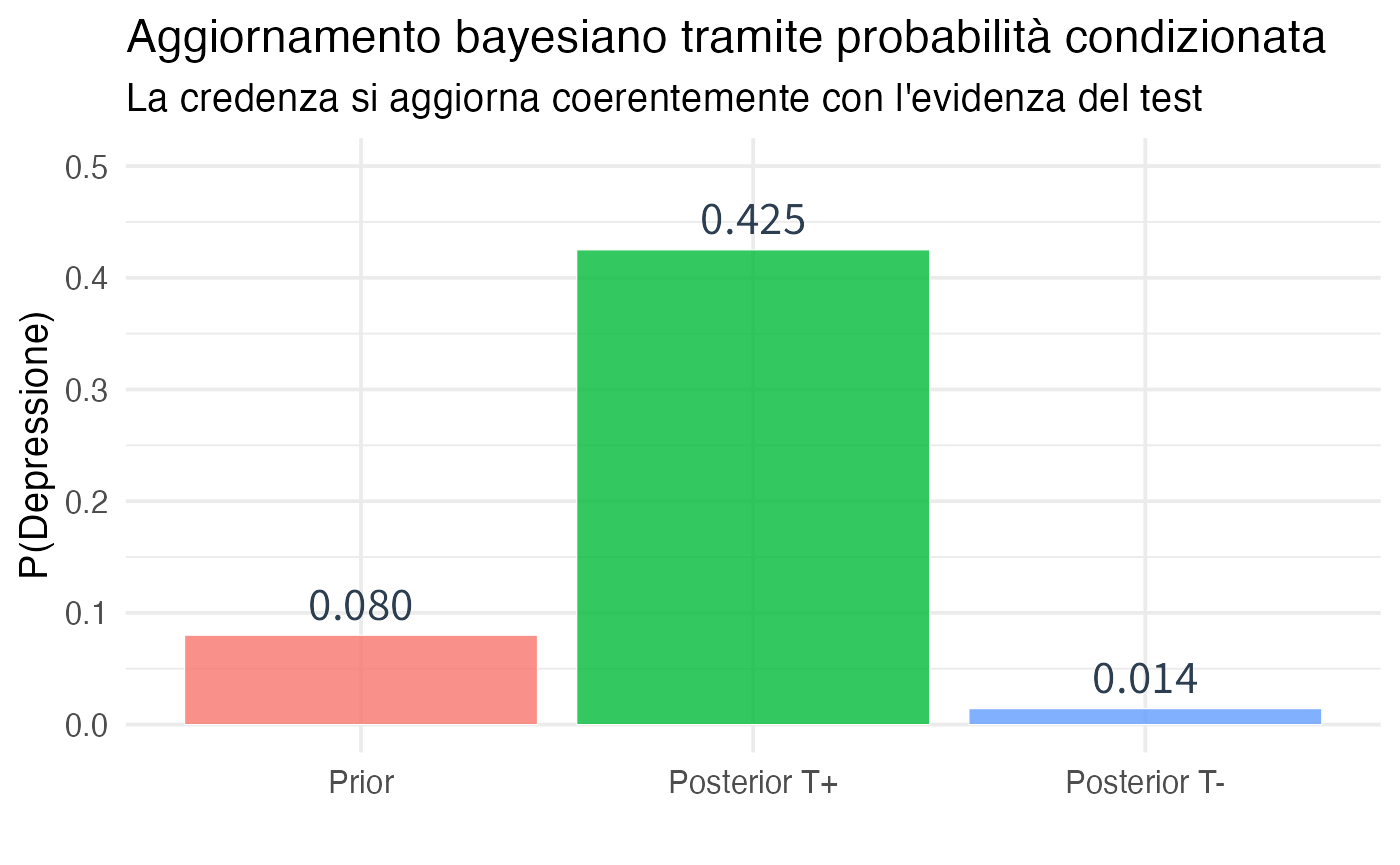
\includegraphics[width=0.85\linewidth,height=\textheight,keepaspectratio]{chapters/probability/04_conditional_prob_bayesian_files/figure-pdf/unnamed-chunk-4-1.png}

\textbf{La lezione epistemica}: lo stesso test può essere molto
informativo in un contesto ad alta prevalenza e quasi inutile in uno a
bassa prevalenza. L'informazione fornita da un test dipende non solo
dalle sue caratteristiche intrinseche, ma anche dal \emph{contesto} in
cui viene applicato.

\end{tcolorbox}

\section{Indipendenza stocastica}\label{sec-independence}

Abbiamo visto che la probabilità condizionata descrive come
l'informazione su un evento modifichi le credenze su un altro. Ma cosa
succede quando l'informazione \emph{non modifica nulla}? Esiste cioè una
situazione in cui apprendere che \(B\) si è verificato lascia inalterata
la nostra credenza in \(A\)?

La risposta è sì, e definisce il concetto di \textbf{indipendenza
stocastica}.

\begin{definition}[Indipendenza (definizione
epistemica)]\protect\hypertarget{def-independence}{}\label{def-independence}

Due eventi \(A\) e \(B\) sono detti \textbf{indipendenti} (notazione:
\(A \perp B\)) se l'informazione che uno dei due si è verificato non
modifica la credenza relativa all'altro:

\[
P(A \mid B) = P(A),
\] e, in modo equivalente,

\[
P(B \mid A) = P(B).
\]

\end{definition}

\subsection{L'indipendenza è epistemica, non
causale}\label{lindipendenza-uxe8-epistemica-non-causale}

È importante chiarire subito un potenziale fraintendimento.
L'indipendenza stocastica è un concetto \textbf{epistemico}, non
causale. Affermare che \(A\) e \(B\) sono indipendenti non significa che
non esistano relazioni causali tra loro, ma che, \textbf{date le
informazioni in nostro possesso}, sapere che uno si è verificato non
fornisce alcuna informazione sull'altro.

Un esempio classico è il lancio di due monete equilibrate. Sapere che la
prima è uscita testa non modifica la credenza che la seconda uscirà
testa. Ma questo non è un fatto ``della natura'' --- è una conseguenza
del nostro stato informativo: sappiamo che i lanci sono fisicamente
indipendenti e che non esistono informazioni nascoste che li colleghino.
Se sospettassimo che una delle monete sia truccata, l'indipendenza
verrebbe meno, perché l'esito della prima lancerebbe un'ombra
sull'affidabilità della seconda.

\subsection{La fattorizzazione come
conseguenza}\label{la-fattorizzazione-come-conseguenza}

Dalla definizione segue immediatamente una proprietà algebrica
fondamentale:

\begin{equation}\protect\phantomsection\label{eq-independence-factorization}{
P(A \cap B) = P(A) \cdot P(B).
}\end{equation}

Questa relazione è spesso presentata nei manuali come \emph{definizione}
di indipendenza, ma è più illuminante considerarla come una
\emph{conseguenza} della definizione epistemica. La fattorizzazione ci
dice che la probabilità congiunta si ``scompone'' nel prodotto delle
marginali: non c'è nulla nella distribuzione congiunta che non sia già
catturato dalle marginali separate. L'informazione non scorre tra i due
eventi.

\begin{tcolorbox}[enhanced jigsaw, arc=.35mm, bottomrule=.15mm, bottomtitle=1mm, breakable, colback=white, colbacktitle=quarto-callout-warning-color!10!white, colframe=quarto-callout-warning-color-frame, coltitle=black, left=2mm, leftrule=.75mm, opacityback=0, opacitybacktitle=0.6, rightrule=.15mm, title=\textcolor{quarto-callout-warning-color}{\faExclamationTriangle}\hspace{0.5em}{Un errore comune: confondere disgiunzione e indipendenza}, titlerule=0mm, toprule=.15mm, toptitle=1mm]

Due eventi \textbf{disgiunti} (mutualmente esclusivi) \textbf{non
possono essere indipendenti}, a meno che uno dei due abbia probabilità
zero.

\textbf{Perché?} Se \(A \cap B = \varnothing\) e \(P(A) > 0\),
\(P(B) > 0\), allora:

\[P(A \cap B) = 0, \quad\text{mentre}\quad P(A) \cdot P(B) > 0.\]

La fattorizzazione fallisce clamorosamente.

\textbf{Interpretazione epistemica}: eventi disgiunti sono
\emph{massimamente dipendenti}. Se so che si è verificato \(A\), so con
certezza che \(B\) non si è verificato. Non esiste informazione più
forte di questa. L'indipendenza, al contrario, è l'assenza totale di
informazione reciproca.

\textbf{Esempio clinico}: consideriamo due diagnosi mutualmente
esclusive, come ``Disturbo Bipolare'' e ``Schizofrenia''. Sapere che un
paziente ha ricevuto la prima diagnosi fornisce un'informazione decisiva
sulla seconda (non può averla, almeno in questo quadro nosologico). I
due eventi sono quindi \textbf{profondamente dipendenti}, non
indipendenti.

\end{tcolorbox}

\subsection{Un esempio: il test
diagnostico}\label{un-esempio-il-test-diagnostico}

Torniamo al test diagnostico per la depressione discusso nella sezione
precedente. Test e stato sono (fortunatamente!) dipendenti: un test che
fosse indipendente dallo stato sarebbe clinicamente inutile.

Verifichiamolo numericamente:

\begin{Shaded}
\begin{Highlighting}[]
\CommentTok{\# Parametri noti (dalla sezione precedente)}
\NormalTok{P\_D }\OtherTok{\textless{}{-}} \FloatTok{0.08}
\NormalTok{P\_Tpos }\OtherTok{\textless{}{-}} \FloatTok{0.216}   \CommentTok{\# calcolato in precedenza}
\NormalTok{P\_D\_and\_Tpos }\OtherTok{\textless{}{-}} \FloatTok{0.068}

\CommentTok{\# Se fossero indipendenti}
\NormalTok{P\_D\_indep }\OtherTok{\textless{}{-}}\NormalTok{ P\_D }\SpecialCharTok{*}\NormalTok{ P\_Tpos}

\FunctionTok{cat}\NormalTok{(}\StringTok{"P(D) × P(T+) ="}\NormalTok{, }\FunctionTok{round}\NormalTok{(P\_D\_indep, }\DecValTok{4}\NormalTok{), }\StringTok{"}\SpecialCharTok{\textbackslash{}n}\StringTok{"}\NormalTok{)}
\CommentTok{\#\textgreater{} P(D) × P(T+) = 0.0173}
\FunctionTok{cat}\NormalTok{(}\StringTok{"P(D ∩ T+) osservato ="}\NormalTok{, }\FunctionTok{round}\NormalTok{(P\_D\_and\_Tpos, }\DecValTok{4}\NormalTok{), }\StringTok{"}\SpecialCharTok{\textbackslash{}n}\StringTok{"}\NormalTok{)}
\CommentTok{\#\textgreater{} P(D ∩ T+) osservato = 0.068}
\FunctionTok{cat}\NormalTok{(}\StringTok{"Differenza:"}\NormalTok{, }\FunctionTok{round}\NormalTok{(P\_D\_and\_Tpos }\SpecialCharTok{{-}}\NormalTok{ P\_D\_indep, }\DecValTok{4}\NormalTok{), }\StringTok{"}\SpecialCharTok{\textbackslash{}n}\StringTok{"}\NormalTok{)}
\CommentTok{\#\textgreater{} Differenza: 0.0507}
\end{Highlighting}
\end{Shaded}

La differenza è sostanziale: \(P(D \cap T^+) = 0.068\), mentre il
prodotto delle marginali è \(0.08 \times 0.216 \approx 0.017\). Il test
e la depressione sono quindi \textbf{dipendenti} --- proprio come ci
aspettiamo da uno strumento diagnostico utile.

\subsection{Il test di indipendenza nella
pratica}\label{il-test-di-indipendenza-nella-pratica}

Quando disponiamo di una tabella di probabilità congiunta, possiamo
verificare l'indipendenza con un semplice confronto: calcoliamo la
probabilità congiunta osservata \(P(A \cap B)\) e la confrontiamo con il
prodotto delle marginali \(P(A) \cdot P(B)\). Se coincidono (o sono
molto vicine, nel caso di stime empiriche), gli eventi sono
indipendenti. In caso contrario, c'è informazione reciproca.

Nella pratica psicologica, tuttavia, è importante ricordare che
l'indipendenza è spesso un'\textbf{assunzione}, non un dato di fatto.
Quando costruiamo modelli statistici, assumiamo indipendenza tra
osservazioni, tra item di un test o tra errori di misurazione. Tali
assunzioni vanno giustificate teoricamente e verificate empiricamente,
perché la loro violazione può portare a stime distorte e a conclusioni
errate. L'indipendenza è uno strumento potente, ma va maneggiato con la
consapevolezza che, nei fenomeni psicologici, la dipendenza è spesso la
regola, non l'eccezione.

\section{Teorema del prodotto (regola della
catena)}\label{sec-product-rule}

Il \textbf{teorema del prodotto} ci permette di costruire probabilità
congiunte a partire da componenti più semplici.

\begin{theorem}[Teorema del
prodotto]\protect\hypertarget{thm-product-rule}{}\label{thm-product-rule}

Per due eventi \(A\) e \(B\) con \(P(B) > 0\):

\[
P(A \cap B) = P(A \mid B) \cdot P(B).
\]

Per simmetria:

\[
P(A \cap B) = P(B \mid A) \cdot P(A).
\]

\end{theorem}

\subsection{Interpretazione
sequenziale}\label{interpretazione-sequenziale}

Il teorema ci dice che la probabilità congiunta può essere pensata come
un processo \emph{sequenziale}:

\begin{enumerate}
\def\labelenumi{\arabic{enumi}.}
\tightlist
\item
  valutiamo la probabilità che \(B\) sia vero: \(P(B)\);
\item
  valutiamo la probabilità che \(A\) sia vero \emph{dato che} \(B\) è
  vero: \(P(A \mid B)\);
\item
  la probabilità che \emph{entrambi} siano veri è il prodotto.
\end{enumerate}

Questa scomposizione riflette un modo naturale di costruire modelli
complessi.

\subsection{La regola della catena:
generalizzazione}\label{la-regola-della-catena-generalizzazione}

Il teorema si estende a sequenze di eventi:

\[
\begin{aligned}
P(A_1 \cap A_2 \cap \cdots \cap A_n)
&= P(A_1)\, P(A_2 \mid A_1) \\
&\quad \cdot P(A_3 \mid A_1 \cap A_2) \cdots \\
&\quad \cdot P(A_n \mid A_1 \cap \cdots \cap A_{n-1}).
\end{aligned}
\]

Ogni fattore condiziona su tutto ciò che ``viene prima''. È il modo in
cui funziona l'aggiornamento sequenziale delle credenze.

\section{Legge della probabilità totale}\label{sec-total-probability}

La \textbf{legge della probabilità totale} risponde a una domanda
frequente: come calcolare la probabilità di un evento che può
verificarsi attraverso \emph{scenari alternativi}?

\begin{theorem}[Legge della probabilità
totale]\protect\hypertarget{thm-total-probability}{}\label{thm-total-probability}

Sia \(\{B_1, B_2, \ldots, B_n\}\) una \textbf{partizione} di \(\Omega\)
(eventi mutuamente esclusivi e collettivamente esaustivi). Allora:

\[
P(A) = \sum_{i=1}^{n} P(A \mid B_i) P(B_i).
\]

\end{theorem}

\subsection{Interpretazione
epistemica}\label{interpretazione-epistemica}

La formula racchiude un principio di ragionamento universale: \textbf{la
probabilità totale si ottiene considerando tutti i modi alternativi in
cui l'evento può verificarsi}.

\begin{itemize}
\tightlist
\item
  \(P(A \mid B_i)\): ``Se ci troviamo nello scenario \(B_i\), quanto è
  probabile \(A\)?'';
\item
  \(P(B_i)\): ``Qual è la probabilità che ci si trovi proprio nello
  scenario \(B_i\)?''.
\end{itemize}

È il modo matematicamente corretto di ``fare un passo indietro'' quando
la risposta diretta è ``Dipende dal contesto''.

\subsection{Applicazione: trattare popolazioni
eterogenee}\label{applicazione-trattare-popolazioni-eterogenee}

In contesti reali, i pazienti provengono spesso da sottopopolazioni con
rischi di base molto diversi. Immaginiamo un test per la depressione
somministrato a due gruppi:

{\def\LTcaptype{none} % do not increment counter
\begin{longtable}[]{@{}lll@{}}
\toprule\noalign{}
Fonte del Paziente & Proporzione & Prevalenza \\
\midrule\noalign{}
\endhead
\bottomrule\noalign{}
\endlastfoot
Clinica Specialistica & 30\% & 40\% \\
Popolazione Generale & 70\% & 5\% \\
\end{longtable}
}

Test: sensibilità = 0.85, specificità = 0.90.

\textbf{Calcolo del tasso di positività in ogni sottogruppo}:

\begin{itemize}
\tightlist
\item
  Clinica specialistica: \(0.85 \times 0.40 + 0.10 \times 0.60 = 0.40\)
\item
  Popolazione generale: \(0.85 \times 0.05 + 0.10 \times 0.95 = 0.1375\)
\end{itemize}

\textbf{Tasso complessivo} (legge della probabilità totale):

\[
P(T^+) = 0.40 \times 0.30 + 0.1375 \times 0.70 \approx 0.216
\]

\textbf{Implicazione clinica}: un test positivo in una clinica
specialistica (tasso 40\%) ha un significato predittivo molto diverso
rispetto a un test positivo nella popolazione generale (tasso 13.75\%).
La prevalenza è parte integrante del risultato.

\section{Paradosso di Simpson}\label{sec-simpsons-paradox}

Il \textbf{paradosso di Simpson} è uno degli esempi più istruttivi di
come un'aggregazione ingenua possa condurre a conclusioni opposte
rispetto a quelle valide a livello disaggregato.

\subsection{Il fenomeno}\label{il-fenomeno}

Il paradosso si manifesta quando una relazione statistica osservata tra
due variabili \textbf{si inverte} una volta che i dati vengono
analizzati separatamente all'interno di sottogruppi rilevanti.

\begin{tcolorbox}[enhanced jigsaw, arc=.35mm, bottomrule=.15mm, bottomtitle=1mm, breakable, colback=white, colbacktitle=quarto-callout-note-color!10!white, colframe=quarto-callout-note-color-frame, coltitle=black, left=2mm, leftrule=.75mm, opacityback=0, opacitybacktitle=0.6, rightrule=.15mm, title=\textcolor{quarto-callout-note-color}{\faInfo}\hspace{0.5em}{Esempio: efficacia di un trattamento per la depressione}, titlerule=0mm, toprule=.15mm, toptitle=1mm]

Due cliniche valutano un trattamento. La clinica A tratta casi lievi, la
B casi gravi.

\begin{Shaded}
\begin{Highlighting}[]
\CommentTok{\# Clinica A (casi lievi)}
\NormalTok{n\_A\_trattati }\OtherTok{\textless{}{-}} \DecValTok{90}
\NormalTok{n\_A\_guariti\_trattati }\OtherTok{\textless{}{-}} \DecValTok{81}
\NormalTok{n\_A\_controllo }\OtherTok{\textless{}{-}} \DecValTok{10}
\NormalTok{n\_A\_guariti\_controllo }\OtherTok{\textless{}{-}} \DecValTok{9}

\CommentTok{\# Clinica B (casi gravi)}
\NormalTok{n\_B\_trattati }\OtherTok{\textless{}{-}} \DecValTok{10}
\NormalTok{n\_B\_guariti\_trattati }\OtherTok{\textless{}{-}} \DecValTok{2}
\NormalTok{n\_B\_controllo }\OtherTok{\textless{}{-}} \DecValTok{90}
\NormalTok{n\_B\_guariti\_controllo }\OtherTok{\textless{}{-}} \DecValTok{27}

\CommentTok{\# Proporzioni per clinica}
\NormalTok{prop\_A\_trattati }\OtherTok{\textless{}{-}}\NormalTok{ n\_A\_guariti\_trattati }\SpecialCharTok{/}\NormalTok{ n\_A\_trattati}
\NormalTok{prop\_A\_controllo }\OtherTok{\textless{}{-}}\NormalTok{ n\_A\_guariti\_controllo }\SpecialCharTok{/}\NormalTok{ n\_A\_controllo}
\NormalTok{prop\_B\_trattati }\OtherTok{\textless{}{-}}\NormalTok{ n\_B\_guariti\_trattati }\SpecialCharTok{/}\NormalTok{ n\_B\_trattati}
\NormalTok{prop\_B\_controllo }\OtherTok{\textless{}{-}}\NormalTok{ n\_B\_guariti\_controllo }\SpecialCharTok{/}\NormalTok{ n\_B\_controllo}

\CommentTok{\# Aggregato}
\NormalTok{n\_tot\_trattati }\OtherTok{\textless{}{-}}\NormalTok{ n\_A\_trattati }\SpecialCharTok{+}\NormalTok{ n\_B\_trattati}
\NormalTok{n\_tot\_guariti\_trattati }\OtherTok{\textless{}{-}}\NormalTok{ n\_A\_guariti\_trattati }\SpecialCharTok{+}\NormalTok{ n\_B\_guariti\_trattati}
\NormalTok{n\_tot\_controllo }\OtherTok{\textless{}{-}}\NormalTok{ n\_A\_controllo }\SpecialCharTok{+}\NormalTok{ n\_B\_controllo}
\NormalTok{n\_tot\_guariti\_controllo }\OtherTok{\textless{}{-}}\NormalTok{ n\_A\_guariti\_controllo }\SpecialCharTok{+}\NormalTok{ n\_B\_guariti\_controllo}

\NormalTok{prop\_tot\_trattati }\OtherTok{\textless{}{-}}\NormalTok{ n\_tot\_guariti\_trattati }\SpecialCharTok{/}\NormalTok{ n\_tot\_trattati}
\NormalTok{prop\_tot\_controllo }\OtherTok{\textless{}{-}}\NormalTok{ n\_tot\_guariti\_controllo }\SpecialCharTok{/}\NormalTok{ n\_tot\_controllo}
\end{Highlighting}
\end{Shaded}

\textbf{Risultati per sottogruppo}:

\begin{itemize}
\tightlist
\item
  Clinica A: trattati 90\%, controllo 90\% → nessuna differenza.
\item
  Clinica B: trattati 20\%, controllo 30\% → trattamento
  \emph{peggiore}.
\end{itemize}

In \textbf{nessun sottogruppo} il trattamento risulta superiore.

\textbf{Risultato aggregato}:

\begin{itemize}
\tightlist
\item
  Trattati: 83\%.
\item
  Controllo: 36\%.
\end{itemize}

Nell'analisi aggregata, il trattamento appare \textbf{nettamente
migliore}!

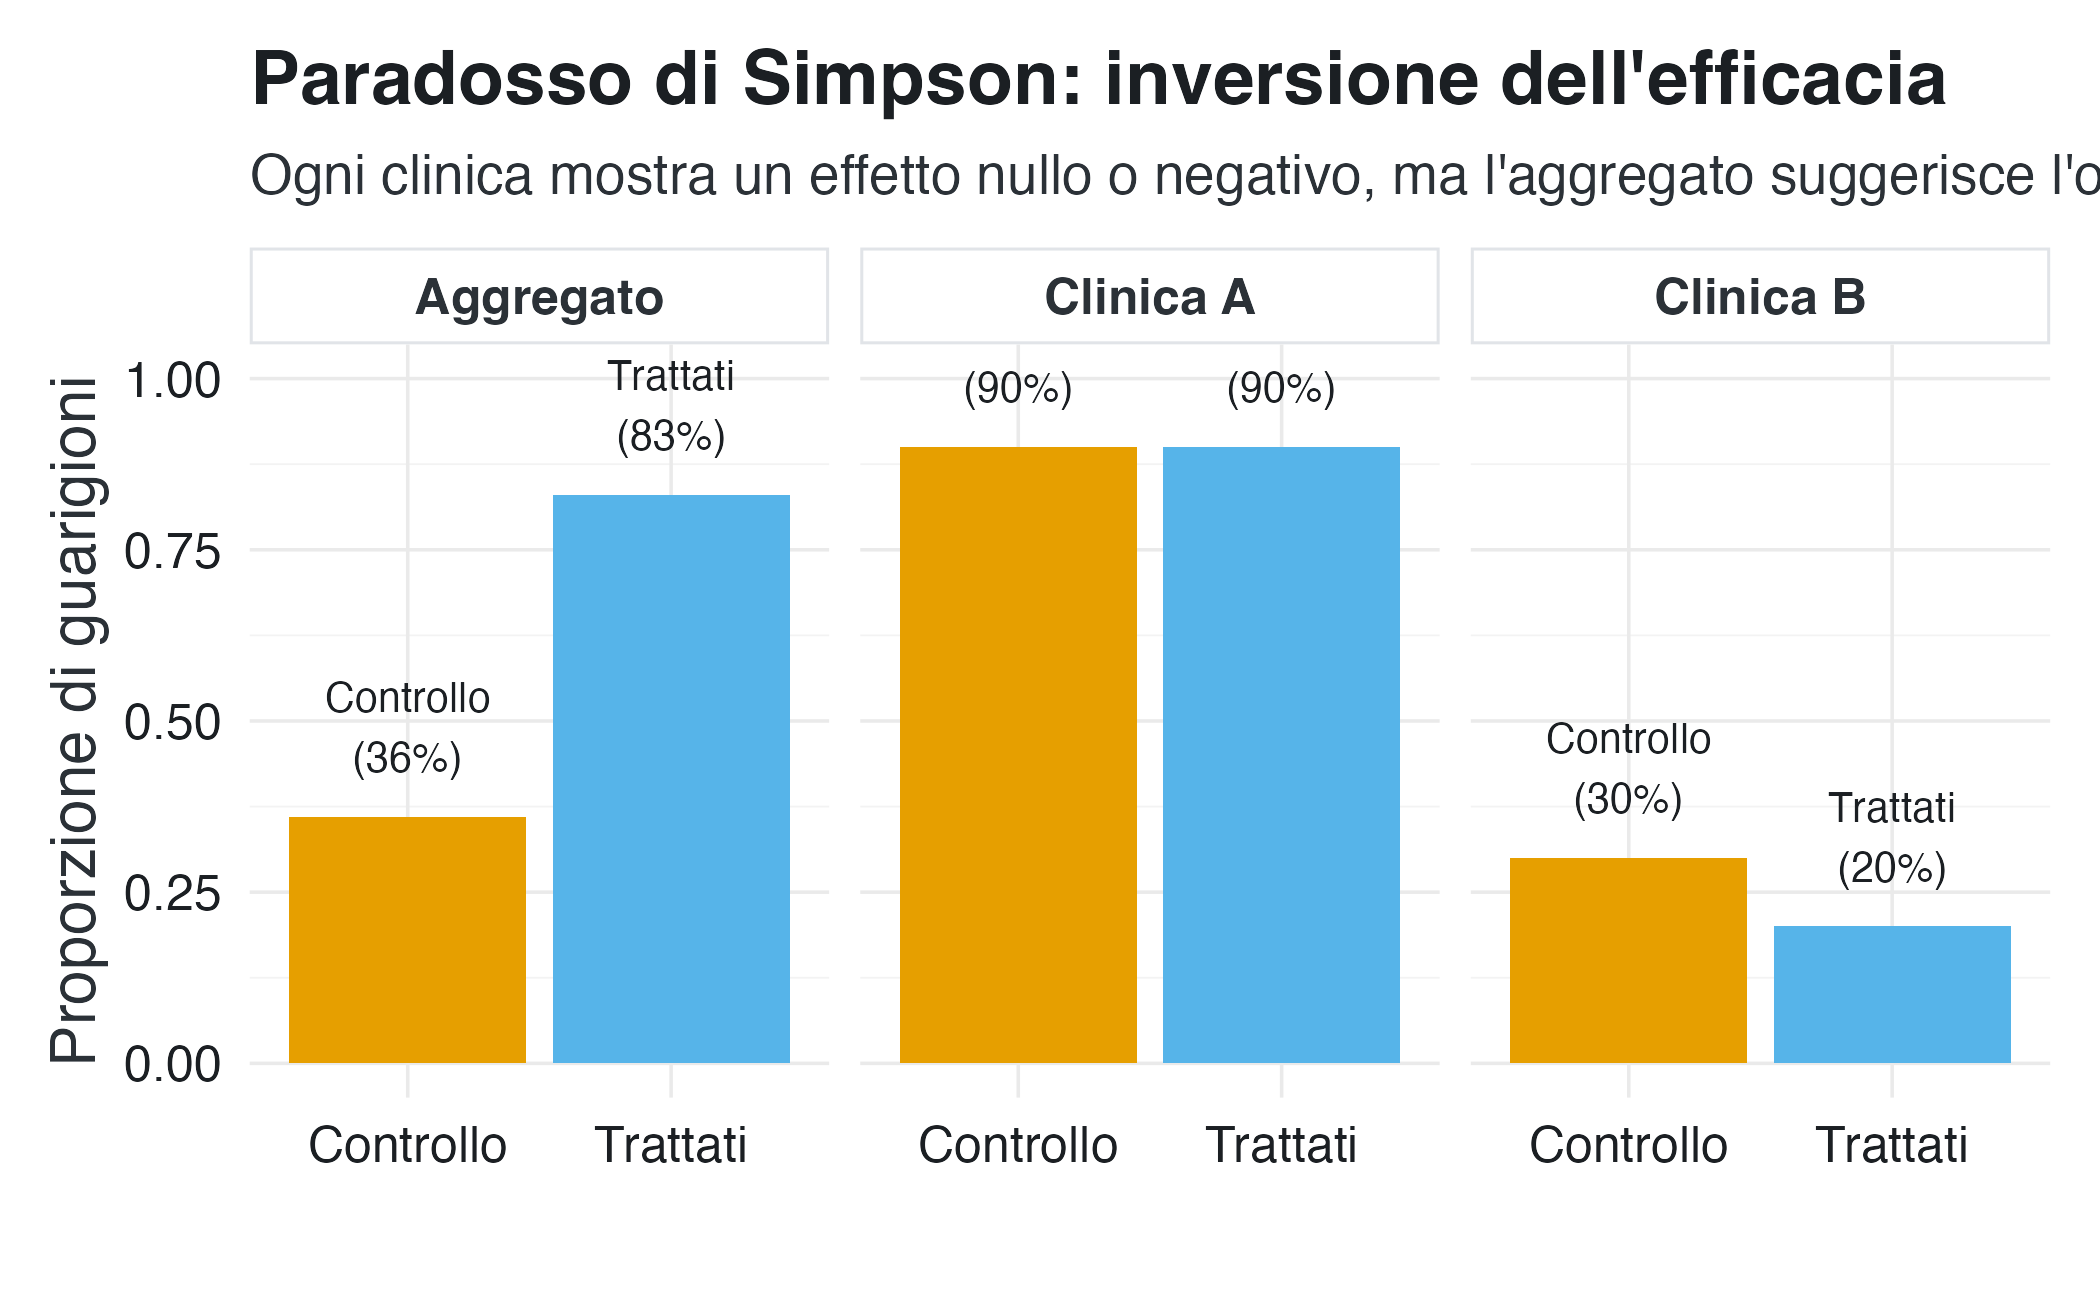
\includegraphics[width=0.85\linewidth,height=\textheight,keepaspectratio]{chapters/probability/04_conditional_prob_bayesian_files/figure-pdf/unnamed-chunk-7-1.png}

\subsection{Cosa sta succedendo?}\label{cosa-sta-succedendo}

La chiave è la \textbf{distribuzione diseguale dei casi}:

\begin{itemize}
\tightlist
\item
  la clinica B (casi gravi, bassa guarigione) contribuisce di più al
  gruppo \emph{trattato};
\item
  la clinica A (casi lievi, alta guarigione) contribuisce di più al
  gruppo \emph{di controllo}.
\end{itemize}

La variabile \emph{gravità} agisce da \textbf{confondente}: influenza
sia la probabilità di ricevere il trattamento sia l'esito.
L'aggregazione ignora questa struttura.

\subsection{La lezione epistemica}\label{la-lezione-epistemica}

L'errore consiste nel rispondere alla \textbf{domanda sbagliata}. Non
stiamo stimando \(P(\text{Guarigione} \mid \text{Trattamento})\), ma una
combinazione implicita di probabilità condizionate diverse. La domanda
corretta è:

\[
P(\text{Guarigione} \mid \text{Trattamento}, \text{Gravità}).
\]

\textbf{Quando è legittimo aggregare?} Solo quando:

\begin{enumerate}
\def\labelenumi{\arabic{enumi}.}
\tightlist
\item
  non esistono confondenti rilevanti;
\item
  i confondenti sono distribuiti uniformemente;
\item
  l'obiettivo è esplicitamente marginale (e non condizionato).
\end{enumerate}

\end{tcolorbox}

\section*{Riflessioni conclusive}\label{riflessioni-conclusive-3}

\markright{Riflessioni conclusive}

Siamo partiti da una domanda apparentemente semplice --- come cambiano
le nostre credenze quando apprendiamo qualcosa di nuovo? --- e abbiamo
scoperto che la risposta richiede un intero apparato concettuale.

\subsection{Cosa abbiamo imparato}\label{cosa-abbiamo-imparato}

La \textbf{probabilità condizionata} è il meccanismo fondamentale
attraverso cui l'informazione si trasforma in conoscenza. Ogni volta che
aggiorniamo le nostre credenze, stiamo implicitamente applicando le
regole che abbiamo studiato.

L'\textbf{indipendenza} rappresenta il caso limite in cui l'informazione
non fluisce. Riconoscere quando questa condizione è soddisfatta è
cruciale per costruire modelli corretti.

Il \textbf{teorema del prodotto} ci ha mostrato come costruire credenze
complesse a partire da componenti più semplici, scomponendo la
probabilità congiunta in una sequenza di aggiornamenti.

La \textbf{legge della probabilità totale} ci ha insegnato a ragionare
su scenari alternativi combinando le probabilità di ciascuno di essi in
una media ponderata.

Il \textbf{paradosso di Simpson} ci ha messo in guardia sui pericoli
dell'aggregazione incauta, mostrando come conclusioni apparentemente
solide possano essere ribaltate quando si svela la struttura nascosta
dei dati.

\subsection{Verso il teorema di Bayes}\label{verso-il-teorema-di-bayes}

Tutti questi strumenti preparano il terreno per il passo successivo.
Abbiamo visto come calcolare \(P(A \mid B)\), ovvero la probabilità di
\(A\) sapendo che si verifica \(B\). Spesso, però, la domanda che ci
interessa è l'inversa: abbiamo osservato un effetto e vogliamo risalire
alla causa.

Nel prossimo capitolo, il \textbf{teorema di Bayes} emergerà come la
regola per questa ``inversione'': passeremo da
\(P(\text{Dati} \mid \text{Ipotesi})\) a
\(P(\text{Ipotesi} \mid \text{Dati})\), il cuore dell'inferenza
scientifica.

\section*{Punti chiave da ricordare}\label{punti-chiave-da-ricordare-3}

\markright{Punti chiave da ricordare}

\begin{tcolorbox}[enhanced jigsaw, arc=.35mm, bottomrule=.15mm, bottomtitle=1mm, breakable, colback=white, colbacktitle=quarto-callout-important-color!10!white, colframe=quarto-callout-important-color-frame, coltitle=black, left=2mm, leftrule=.75mm, opacityback=0, opacitybacktitle=0.6, rightrule=.15mm, title=\textcolor{quarto-callout-important-color}{\faExclamation}\hspace{0.5em}{Importante}, titlerule=0mm, toprule=.15mm, toptitle=1mm]

\begin{enumerate}
\def\labelenumi{\arabic{enumi}.}
\tightlist
\item
  \textbf{Probabilità condizionata come aggiornamento epistemico}

  \begin{itemize}
  \tightlist
  \item
    \(P(A \mid B)\) quantifica la credenza in \(A\) dopo aver appreso
    \(B\).
  \item
    Meccanismo: riduzione dello spazio + rinormalizzazione.
  \item
    Ogni probabilità è sempre condizionata a uno sfondo informativo:
    \(P(A) = P(A \mid \mathcal{I})\).
  \end{itemize}
\item
  \textbf{Indipendenza come assenza di informazione}

  \begin{itemize}
  \tightlist
  \item
    \(A \perp B \iff P(A \mid B) = P(A)\).
  \item
    Equivalentemente: \(P(A \cap B) = P(A) \cdot P(B)\).
  \item
    Eventi disgiunti NON sono indipendenti (hanno informazione reciproca
    massima).
  \end{itemize}
\item
  \textbf{Teorema del prodotto}

  \begin{itemize}
  \tightlist
  \item
    \(P(A \cap B) = P(A \mid B) \cdot P(B) = P(B \mid A) \cdot P(A)\).
  \item
    Generalizzazione: regola della catena per sequenze di eventi.
  \end{itemize}
\item
  \textbf{Legge della probabilità totale}

  \begin{itemize}
  \tightlist
  \item
    \(P(A) = \sum_{i} P(A \mid B_i) P(B_i)\) per partizione \(\{B_i\}\).
  \item
    Fondamentale per ragionare su scenari alternativi.
  \end{itemize}
\item
  \textbf{Paradosso di Simpson}

  \begin{itemize}
  \tightlist
  \item
    Trend aggregati possono invertirsi rispetto a trend stratificati.
  \item
    Avvertimento: condiziona sui confondenti!
  \end{itemize}
\end{enumerate}

\textbf{Formule da ricordare:}

\[
P(A \mid B) = \frac{P(A \cap B)}{P(B)}
\]

\[
P(A \cap B) = P(A \mid B) \cdot P(B) = P(B \mid A) \cdot P(A)
\]

\[
P(A) = \sum_{i=1}^{n} P(A \mid B_i) P(B_i)
\]

\textbf{Per il prossimo capitolo:}

Nel Capitolo~\ref{sec-prob-bayes-theorem} vedremo come il teorema di
Bayes permetta di \textbf{invertire} le probabilità condizionate,
passando da \(P(\text{Dati} \mid \text{Ipotesi})\) a
\(P(\text{Ipotesi} \mid \text{Dati})\).

\end{tcolorbox}

\section*{Esercizi}\label{esercizi-1}

\markright{Esercizi}

\begin{tcolorbox}[enhanced jigsaw, arc=.35mm, bottomrule=.15mm, bottomtitle=1mm, breakable, colback=white, colbacktitle=quarto-callout-important-color!10!white, colframe=quarto-callout-important-color-frame, coltitle=black, left=2mm, leftrule=.75mm, opacityback=0, opacitybacktitle=0.6, rightrule=.15mm, title=\textcolor{quarto-callout-important-color}{\faExclamation}\hspace{0.5em}{Problemi}, titlerule=0mm, toprule=.15mm, toptitle=1mm]

\subsection*{Esercizi concettuali}\label{esercizi-concettuali}

\begin{enumerate}
\def\labelenumi{\arabic{enumi}.}
\item
  Spiega perché ``ogni probabilità è condizionata'' da una prospettiva
  bayesiana. Cosa significa \(P(A)\) implicitamente?
\item
  La formula \(P(A \mid B) = P(A \cap B) / P(B)\) può sembrare
  circolare. Spiega perché non lo è, e in quale ordine concettuale
  pensiamo queste quantità.
\item
  Quando due eventi sono disgiunti, possono essere indipendenti? Perché
  o perché no?
\item
  Il teorema del prodotto dice \(P(A \cap B) = P(A \mid B) P(B)\).
  Questo è simmetrico? Cioè, posso scrivere
  \(P(A \cap B) = P(B \mid A) P(A)\)? Cosa implica questa simmetria?
\item
  Il paradosso di Simpson dimostra che l'aggregazione è sempre
  sbagliata? Quando è legittimo aggregare dati?
\end{enumerate}

\subsection*{Esercizi su probabilità
condizionata}\label{esercizi-su-probabilituxe0-condizionata}

\begin{enumerate}
\def\labelenumi{\arabic{enumi}.}
\setcounter{enumi}{5}
\item
  Data una tabella congiunta: \textbar{} \textbar{} \(B\) \textbar{}
  \(B^c\) \textbar{}
  \textbar-------\textbar------\textbar-------\textbar{} \textbar{}
  \(A\) \textbar{} 0.20 \textbar{} 0.30 \textbar{} \textbar{} \(A^c\)
  \textbar{} 0.15 \textbar{} 0.35 \textbar{}

  Calcola:

  \begin{enumerate}
  \def\labelenumii{\alph{enumii}.}
  \tightlist
  \item
    \(P(A \mid B)\)
  \item
    \(P(B \mid A)\)
  \item
    \(P(A \mid B^c)\)
  \item
    Gli eventi sono indipendenti?
  \end{enumerate}
\item
  \(P(A) = 0.6\), \(P(B) = 0.5\), \(P(A \mid B) = 0.7\). Calcola:

  \begin{enumerate}
  \def\labelenumii{\alph{enumii}.}
  \tightlist
  \item
    \(P(A \cap B)\)
  \item
    \(P(B \mid A)\)
  \item
    \(P(A \cup B)\)
  \end{enumerate}
\item
  Test diagnostico: \(P(M) = 0.01\), sens = 0.95, spec = 0.98.

  \begin{enumerate}
  \def\labelenumii{\alph{enumii}.}
  \tightlist
  \item
    Costruisci tabella congiunta
  \item
    Calcola VPP e VPN
  \item
    Quanto deve essere alta la sensibilità per avere VPP \textgreater{}
    0.9?
  \end{enumerate}
\end{enumerate}

\subsection*{Esercizi
sull'indipendenza}\label{esercizi-sullindipendenza}

\begin{enumerate}
\def\labelenumi{\arabic{enumi}.}
\setcounter{enumi}{8}
\tightlist
\item
  Un dado viene lanciato. Siano:

  \begin{itemize}
  \tightlist
  \item
    \(A\) = ``Esce numero pari''
  \item
    \(B\) = ``Esce numero ≤ 3''
  \end{itemize}

  \begin{enumerate}
  \def\labelenumii{\alph{enumii}.}
  \tightlist
  \item
    \(A\) e \(B\) sono indipendenti?
  \item
    Calcola \(P(A \mid B)\) e confronta con \(P(A)\)
  \end{enumerate}
\item
  Due monete equilibrate vengono lanciate. Siano:

  \begin{itemize}
  \tightlist
  \item
    \(A\) = ``Prima moneta è testa''
  \item
    \(B\) = ``Almeno una testa''
  \end{itemize}

  \begin{enumerate}
  \def\labelenumii{\alph{enumii}.}
  \tightlist
  \item
    Costruisci tabella congiunta
  \item
    Calcola \(P(A \mid B)\)
  \item
    \(A\) e \(B\) sono indipendenti?
  \end{enumerate}
\item
  In una popolazione, \(P(\text{Depressione}) = 0.15\) e
  \(P(\text{Insonnia}) = 0.25\). Se fossero indipendenti, quanto sarebbe
  \(P(\text{Depressione} \cap \text{Insonnia})\)? È plausibile
  l'indipendenza?
\end{enumerate}

\subsection*{Esercizi sul teorema del
prodotto}\label{esercizi-sul-teorema-del-prodotto}

\begin{enumerate}
\def\labelenumi{\arabic{enumi}.}
\setcounter{enumi}{11}
\item
  \(P(A) = 0.5\), \(P(B \mid A) = 0.6\), \(P(C \mid A \cap B) = 0.7\).
  Calcola \(P(A \cap B \cap C)\).
\item
  Tre test sequenziali per ansia, ciascuno con sens = 0.80 (indipendenti
  dato stato). \(P(\text{Ansia}) = 0.20\). Calcola
  \(P(\text{Ansia} \cap T_1^+ \cap T_2^+ \cap T_3^+)\).
\item
  Usa la regola del prodotto per dimostrare che se \(A\) e \(B\) sono
  indipendenti, allora \(A\) e \(B^c\) sono indipendenti.
\end{enumerate}

\subsection*{Esercizi sulla probabilità
totale}\label{esercizi-sulla-probabilituxe0-totale}

\begin{enumerate}
\def\labelenumi{\arabic{enumi}.}
\setcounter{enumi}{14}
\item
  Una clinica riceve pazienti da due fonti:

  \begin{itemize}
  \tightlist
  \item
    60\% da medico di base (prevalenza depressione = 10\%)
  \item
    40\% da pronto soccorso (prevalenza depressione = 30\%)
  \end{itemize}

  Qual è la prevalenza complessiva nella clinica?
\item
  Un questionario ha due versioni (A e B), distribuite casualmente (50\%
  ciascuna). La versione A è più facile:

  \begin{itemize}
  \tightlist
  \item
    \(P(\text{punteggio} > 20 \mid \text{Versione A}) = 0.7\)
  \item
    \(P(\text{punteggio} > 20 \mid \text{Versione B}) = 0.4\)
  \end{itemize}

  Qual è \(P(\text{punteggio} > 20)\) complessivamente?
\item
  Dimostra che \(P(A) = P(A \mid B) P(B) + P(A \mid B^c) P(B^c)\) usando
  la legge della probabilità totale con partizione \(\{B, B^c\}\).
\end{enumerate}

\subsection*{Esercizi sul Paradosso di
Simpson}\label{esercizi-sul-paradosso-di-simpson}

\begin{enumerate}
\def\labelenumi{\arabic{enumi}.}
\setcounter{enumi}{17}
\item
  Considera questi dati su un farmaco antidepressivo:

  \textbf{Pazienti giovani} (N=200):

  \begin{itemize}
  \tightlist
  \item
    Farmaco: 70/100 migliorati (70\%)
  \item
    Placebo: 50/100 migliorati (50\%)
  \end{itemize}

  \textbf{Pazienti anziani} (N=200):

  \begin{itemize}
  \tightlist
  \item
    Farmaco: 60/100 migliorati (60\%)
  \item
    Placebo: 40/100 migliorati (40\%)
  \end{itemize}

  \begin{enumerate}
  \def\labelenumii{\alph{enumii}.}
  \tightlist
  \item
    In ciascun gruppo, il farmaco è migliore?
  \item
    Calcola le proporzioni aggregate (tutti i pazienti insieme)
  \item
    Costruisci uno scenario dove l'aggregato inverte la tendenza
  \end{enumerate}
\item
  Spiega in termini epistemici perché il paradosso di Simpson non è
  veramente un ``paradosso'' ma un avvertimento sull'importanza di
  condizionare correttamente.
\end{enumerate}

\subsection*{Esercizi applicati}\label{esercizi-applicati}

\begin{enumerate}
\def\labelenumi{\arabic{enumi}.}
\setcounter{enumi}{19}
\tightlist
\item
  \textbf{Test per disturbo d'ansia sociale}:

  \begin{itemize}
  \tightlist
  \item
    Prevalenza in popolazione universitaria: 5\%
  \item
    Sensibilità: 85\%
  \item
    Specificità: 92\%
  \end{itemize}

  \begin{enumerate}
  \def\labelenumii{\alph{enumii}.}
  \tightlist
  \item
    Costruisci tabella congiunta completa
  \item
    Uno studente risulta positivo. Qual è la probabilità che abbia
    davvero il disturbo?
  \item
    Quale prevalenza minima serve per avere VPP \textgreater{} 0.5?
  \end{enumerate}
\item
  \textbf{Comorbidità PTSD e Depressione}:

  \begin{itemize}
  \tightlist
  \item
    In un campione clinico: \(P(\text{PTSD}) = 0.30\),
    \(P(\text{Depressione}) = 0.45\)
  \item
    Osservi che \(P(\text{Depressione} \mid \text{PTSD}) = 0.70\)
  \end{itemize}

  \begin{enumerate}
  \def\labelenumii{\alph{enumii}.}
  \tightlist
  \item
    Calcola \(P(\text{PTSD} \cap \text{Depressione})\)
  \item
    Calcola \(P(\text{PTSD} \mid \text{Depressione})\)
  \item
    Sono indipendenti? Commenta il risultato clinicamente
  \end{enumerate}
\item
  \textbf{Due test per ADHD in un bambino}:

  \begin{itemize}
  \tightlist
  \item
    Prior: \(P(\text{ADHD}) = 0.08\) (popolazione generale)
  \item
    Test comportamentale: positivo (sens=0.80, spec=0.90)
  \item
    Test cognitivo: positivo (sens=0.75, spec=0.85)
  \item
    Assumendo indipendenza condizionale:
  \end{itemize}

  \begin{enumerate}
  \def\labelenumii{\alph{enumii}.}
  \tightlist
  \item
    Calcola \(P(\text{ADHD} \mid T_1^+)\) dopo primo test
  \item
    Calcola \(P(\text{ADHD} \mid T_1^+, T_2^+)\) dopo entrambi i test
  \item
    Visualizza l'aggiornamento sequenziale delle credenze
  \end{enumerate}
\end{enumerate}

\subsection*{Esercizi computazionali}\label{esercizi-computazionali-1}

\begin{enumerate}
\def\labelenumi{\arabic{enumi}.}
\setcounter{enumi}{22}
\tightlist
\item
  Scrivi una funzione R che:

  \begin{itemize}
  \tightlist
  \item
    Input: tabella congiunta 2×2
  \item
    Output: tutte le probabilità condizionate possibili e test di
    indipendenza
  \end{itemize}
\item
  Simula il paradosso di Simpson:

  \begin{itemize}
  \tightlist
  \item
    Genera dati per due gruppi con trend positivo in ciascuno
  \item
    Aggrega i dati mostrando inversione del trend
  \item
    Visualizza con ggplot
  \end{itemize}
\item
  Crea una visualizzazione interattiva (o animazione) che mostra come
  \(P(A \mid B)\) varia al variare della ``forza'' dell'associazione tra
  \(A\) e \(B\) (da indipendenza a dipendenza totale).
\end{enumerate}

\end{tcolorbox}

\begin{tcolorbox}[enhanced jigsaw, arc=.35mm, bottomrule=.15mm, bottomtitle=1mm, breakable, colback=white, colbacktitle=quarto-callout-tip-color!10!white, colframe=quarto-callout-tip-color-frame, coltitle=black, left=2mm, leftrule=.75mm, opacityback=0, opacitybacktitle=0.6, rightrule=.15mm, title=\textcolor{quarto-callout-tip-color}{\faLightbulb}\hspace{0.5em}{Soluzioni selezionate}, titlerule=0mm, toprule=.15mm, toptitle=1mm]

\subsection*{Soluzioni degli esercizi
concettuali}\label{soluzioni-degli-esercizi-concettuali}

\begin{enumerate}
\def\labelenumi{\arabic{enumi}.}
\item
  Da prospettiva bayesiana, ogni probabilità riflette uno stato di
  informazione. Scrivere \(P(A)\) è abbreviazione per
  \(P(A \mid \mathcal{I})\) dove \(\mathcal{I}\) è ``tutto ciò che
  sappiamo''. Non esistono probabilità ``incondizionate''---solo
  probabilità condizionate allo sfondo informativo corrente.
\item
  Non è circolare perché concettualmente partiamo dalla \textbf{tabella
  congiunta} \(P(A \cap B)\) (rappresentazione completa del nostro stato
  di credenza), poi \textbf{deriviamo} le condizionate come rapporti. La
  formula ci dice \emph{come calcolare} condizionate da congiunte, non
  \emph{come definire} le congiunte.
\item
  No (a meno che uno abbia probabilità zero). Eventi disgiunti hanno
  informazione reciproca \textbf{massima}: sapere che uno è vero implica
  certezza che l'altro è falso. Indipendenza richiede \emph{assenza} di
  informazione.
\item
  Sì, è simmetrico:
  \(P(A \cap B) = P(A \mid B) P(B) = P(B \mid A) P(A)\). Questa
  simmetria è il cuore del teorema di Bayes! Mostra che la congiunta può
  essere costruita in due modi equivalenti.
\item
  No, l'aggregazione è legittima quando non c'è confondente rilevante, o
  quando la confondente è distribuita uniformemente. Il paradosso
  avverte: \emph{esplicita le tue assunzioni di omogeneità prima di
  aggregare}.
\end{enumerate}

\subsection*{Soluzioni degli esercizi sulla probabilità
condizionata}\label{soluzioni-degli-esercizi-sulla-probabilituxe0-condizionata}

\begin{enumerate}
\def\labelenumi{\arabic{enumi}.}
\setcounter{enumi}{5}
\tightlist
\item
  \begin{enumerate}
  \def\labelenumii{\alph{enumii}.}
  \tightlist
  \item
    \(P(A \mid B) = 0.20 / (0.20 + 0.15) = 0.571\)
  \item
    \(P(B \mid A) = 0.20 / (0.20 + 0.30) = 0.400\)
  \item
    \(P(A \mid B^c) = 0.30 / (0.30 + 0.35) = 0.462\)
  \item
    Test: \(P(A) = 0.50\), \(P(B) = 0.35\),
    \(P(A) P(B) = 0.175 \neq P(A \cap B) = 0.20\). NON indipendenti.
  \end{enumerate}
\item
  \begin{enumerate}
  \def\labelenumii{\alph{enumii}.}
  \tightlist
  \item
    \(P(A \cap B) = P(A \mid B) P(B) = 0.7 \times 0.5 = 0.35\)
  \item
    \(P(B \mid A) = P(A \cap B) / P(A) = 0.35 / 0.6 \approx 0.583\)
  \item
    \(P(A \cup B) = 0.6 + 0.5 - 0.35 = 0.75\)
  \end{enumerate}
\item
  \begin{enumerate}
  \def\labelenumii{\alph{enumii}.}
  \tightlist
  \item
    Tabella: \(P(M \cap T^+) = 0.0095\), \(P(M \cap T^-) = 0.0005\),
    etc.
  \item
    VPP = \(0.0095 / (0.0095 + 0.0198) \approx 0.324\); VPN
    \(\approx 0.9995\)
  \item
    Per VPP \textgreater{} 0.9: serve sens \(\approx 0.998\) (quasi
    perfetta con prevalenza così bassa!)
  \end{enumerate}
\end{enumerate}

\subsection*{Soluzioni degli esercizi
sull'indipendenza}\label{soluzioni-degli-esercizi-sullindipendenza}

\begin{enumerate}
\def\labelenumi{\arabic{enumi}.}
\setcounter{enumi}{8}
\tightlist
\item
  \begin{enumerate}
  \def\labelenumii{\alph{enumii}.}
  \tightlist
  \item
    \(P(A) = 1/2\), \(P(B) = 1/2\), \(P(A \cap B) = P(\{2\}) = 1/6\)
    \(P(A) P(B) = 1/4 \neq 1/6\). NON indipendenti.
  \item
    \(P(A \mid B) = (1/6) / (1/2) = 1/3 \neq 1/2 = P(A)\)
  \end{enumerate}
\item
  Spazio: \{TT, TC, CT, CC\}, equiprobabili.

  \begin{enumerate}
  \def\labelenumii{\alph{enumii}.}
  \tightlist
  \item
    Tabella con \(A\) = \{TT, TC\}, \(B\) = \{TT, TC, CT\}
  \item
    \(P(A \mid B) = P(\{TT, TC\}) / P(B) = (1/2) / (3/4) = 2/3\)
  \item
    \(P(A) = 1/2 \neq 2/3 = P(A \mid B)\). NON indipendenti.
  \end{enumerate}
\item
  Se indipendenti: \(P(D \cap I) = 0.15 \times 0.25 = 0.0375\). Ma
  clinicamente sappiamo che depressione e insonnia sono altamente
  correlate, quindi l'indipendenza è \textbf{implausibile}.
\end{enumerate}

\subsection*{Soluzioni degli esercizi sul teorema del
prodotto}\label{soluzioni-degli-esercizi-sul-teorema-del-prodotto}

\begin{enumerate}
\def\labelenumi{\arabic{enumi}.}
\setcounter{enumi}{11}
\item
  \(P(A \cap B \cap C) = P(C \mid A \cap B) \cdot P(B \mid A) \cdot P(A) = 0.7 \times 0.6 \times 0.5 = 0.21\)
\item
  \(P(\text{Ansia} \cap \text{tutti +}) = 0.80^3 \times 0.20 = 0.512 \times 0.20 = 0.1024\)
\item
  Dimostrazione:

\begin{verbatim}
P(A ∩ B^c) = P(A) - P(A ∩ B)    [additività]
           = P(A) - P(A)P(B)     [indipendenza A,B]
           = P(A)(1 - P(B))
           = P(A)P(B^c)          [quindi A ⊥ B^c]
\end{verbatim}
\end{enumerate}

\subsection*{Soluzioni degli esercizi sulla probabilità
totale}\label{soluzioni-degli-esercizi-sulla-probabilituxe0-totale}

\begin{enumerate}
\def\labelenumi{\arabic{enumi}.}
\setcounter{enumi}{14}
\item
  \(P(D) = 0.10 \times 0.60 + 0.30 \times 0.40 = 0.06 + 0.12 = 0.18\)
  (18\%)
\item
  \(P(>20) = 0.7 \times 0.5 + 0.4 \times 0.5 = 0.35 + 0.20 = 0.55\)
\end{enumerate}

\subsection*{Soluzioni degli esercizi sulle applicazioni
psicologiche}\label{soluzioni-degli-esercizi-sulle-applicazioni-psicologiche}

\begin{enumerate}
\def\labelenumi{\arabic{enumi}.}
\setcounter{enumi}{19}
\tightlist
\item
  \begin{enumerate}
  \def\labelenumii{\alph{enumii}.}
  \tightlist
  \item
    \(P(A \cap T^+) = 0.85 \times 0.05 = 0.0425\), etc.
  \item
    VPP = \(0.0425 / (0.0425 + 0.076) = 0.359\) (solo 36\%!)
  \item
    Per VPP \textgreater{} 0.5, serve prev \(\geq 0.10\) (10\%)
  \end{enumerate}
\item
  \begin{enumerate}
  \def\labelenumii{\alph{enumii}.}
  \tightlist
  \item
    \(P(P \cap D) = P(D \mid P) \times P(P) = 0.70 \times 0.30 = 0.21\)
  \item
    \(P(P \mid D) = 0.21 / 0.45 \approx 0.467\)
  \item
    Se indipendenti: \(P(P) P(D) = 0.30 \times 0.45 = 0.135 \neq 0.21\).
    DIPENDENTI (comorbidità alta, clinicamente attesa)
  \end{enumerate}
\end{enumerate}

\end{tcolorbox}

\begin{tcolorbox}[enhanced jigsaw, arc=.35mm, bottomrule=.15mm, bottomtitle=1mm, breakable, colback=white, colbacktitle=quarto-callout-note-color!10!white, colframe=quarto-callout-note-color-frame, coltitle=black, left=2mm, leftrule=.75mm, opacityback=0, opacitybacktitle=0.6, rightrule=.15mm, title=\textcolor{quarto-callout-note-color}{\faInfo}\hspace{0.5em}{Informazioni sull'ambiente di sviluppo}, titlerule=0mm, toprule=.15mm, toptitle=1mm]

\begin{Shaded}
\begin{Highlighting}[]
\FunctionTok{sessionInfo}\NormalTok{()}
\CommentTok{\#\textgreater{} R version 4.6.1 (2026{-}06{-}24)}
\CommentTok{\#\textgreater{} Platform: aarch64{-}apple{-}darwin23}
\CommentTok{\#\textgreater{} Running under: macOS Tahoe 26.5.2}
\CommentTok{\#\textgreater{} }
\CommentTok{\#\textgreater{} Matrix products: default}
\CommentTok{\#\textgreater{} BLAS:   /Library/Frameworks/R.framework/Versions/4.6/Resources/lib/libRblas.0.dylib }
\CommentTok{\#\textgreater{} LAPACK: /Library/Frameworks/R.framework/Versions/4.6/Resources/lib/libRlapack.dylib;  LAPACK version 3.12.1}
\CommentTok{\#\textgreater{} }
\CommentTok{\#\textgreater{} locale:}
\CommentTok{\#\textgreater{} [1] C.UTF{-}8/UTF{-}8/C.UTF{-}8/C/C.UTF{-}8/C.UTF{-}8}
\CommentTok{\#\textgreater{} }
\CommentTok{\#\textgreater{} time zone: Europe/Rome}
\CommentTok{\#\textgreater{} tzcode source: internal}
\CommentTok{\#\textgreater{} }
\CommentTok{\#\textgreater{} attached base packages:}
\CommentTok{\#\textgreater{} [1] stats     graphics  grDevices utils     datasets  methods   base     }
\CommentTok{\#\textgreater{} }
\CommentTok{\#\textgreater{} other attached packages:}
\CommentTok{\#\textgreater{}  [1] ggforce\_0.5.0         ragg\_1.5.2            tinytable\_0.17.0     }
\CommentTok{\#\textgreater{}  [4] withr\_3.0.3           systemfonts\_1.3.2     patchwork\_1.3.2      }
\CommentTok{\#\textgreater{}  [7] ggdist\_3.3.3          tidybayes\_3.0.7       bayesplot\_1.15.0     }
\CommentTok{\#\textgreater{} [10] ggplot2\_4.0.3         reliabilitydiag\_0.2.1 priorsense\_1.2.0     }
\CommentTok{\#\textgreater{} [13] posterior\_1.7.0       loo\_2.10.0            rstan\_2.32.7         }
\CommentTok{\#\textgreater{} [16] StanHeaders\_2.32.10   brms\_2.23.0           Rcpp\_1.1.2           }
\CommentTok{\#\textgreater{} [19] sessioninfo\_1.2.4     conflicted\_1.2.0      janitor\_2.2.1        }
\CommentTok{\#\textgreater{} [22] matrixStats\_1.5.0     modelr\_0.1.11         tibble\_3.3.1         }
\CommentTok{\#\textgreater{} [25] dplyr\_1.2.1           tidyr\_1.3.2           rio\_1.3.0            }
\CommentTok{\#\textgreater{} [28] here\_1.0.2           }
\CommentTok{\#\textgreater{} }
\CommentTok{\#\textgreater{} loaded via a namespace (and not attached):}
\CommentTok{\#\textgreater{}  [1] svUnit\_1.0.8          tidyselect\_1.2.1      farver\_2.1.2         }
\CommentTok{\#\textgreater{}  [4] S7\_0.2.2              fastmap\_1.2.0         tensorA\_0.36.2.1     }
\CommentTok{\#\textgreater{}  [7] tweenr\_2.0.3          pacman\_0.5.1          digest\_0.6.39        }
\CommentTok{\#\textgreater{} [10] timechange\_0.4.0      estimability\_2.0.0    lifecycle\_1.0.5      }
\CommentTok{\#\textgreater{} [13] magrittr\_2.0.5        compiler\_4.6.1        rlang\_1.3.0          }
\CommentTok{\#\textgreater{} [16] tools\_4.6.1           yaml\_2.3.12           knitr\_1.51           }
\CommentTok{\#\textgreater{} [19] labeling\_0.4.3        bridgesampling\_1.2{-}1  pkgbuild\_1.4.8       }
\CommentTok{\#\textgreater{} [22] curl\_7.1.0            RColorBrewer\_1.1{-}3    abind\_1.4{-}8          }
\CommentTok{\#\textgreater{} [25] purrr\_1.2.2           polyclip\_1.10{-}7       grid\_4.6.1           }
\CommentTok{\#\textgreater{} [28] stats4\_4.6.1          xtable\_1.8{-}8          inline\_0.3.21        }
\CommentTok{\#\textgreater{} [31] MASS\_7.3{-}65           emmeans\_2.0.3         scales\_1.4.0         }
\CommentTok{\#\textgreater{} [34] cli\_3.6.6             mvtnorm\_1.4{-}1         rmarkdown\_2.31       }
\CommentTok{\#\textgreater{} [37] generics\_0.1.4        otel\_0.2.0            RcppParallel\_5.1.11{-}2}
\CommentTok{\#\textgreater{} [40] cachem\_1.1.0          stringr\_1.6.0         parallel\_4.6.1       }
\CommentTok{\#\textgreater{} [43] vctrs\_0.7.3           V8\_8.2.0              Matrix\_1.7{-}5         }
\CommentTok{\#\textgreater{} [46] jsonlite\_2.0.0        arrayhelpers\_1.1{-}1    glue\_1.8.1           }
\CommentTok{\#\textgreater{} [49] codetools\_0.2{-}20      distributional\_0.8.1  lubridate\_1.9.5      }
\CommentTok{\#\textgreater{} [52] stringi\_1.8.7         gtable\_0.3.6          QuickJSR\_1.10.0      }
\CommentTok{\#\textgreater{} [55] pillar\_1.11.1         htmltools\_0.5.9       Brobdingnag\_1.2{-}9    }
\CommentTok{\#\textgreater{} [58] R6\_2.6.1              textshaping\_1.0.5     rprojroot\_2.1.1      }
\CommentTok{\#\textgreater{} [61] evaluate\_1.0.5        lattice\_0.22{-}9        backports\_1.5.1      }
\CommentTok{\#\textgreater{} [64] memoise\_2.0.1         broom\_1.0.13          snakecase\_0.11.1     }
\CommentTok{\#\textgreater{} [67] rstantools\_2.6.0      coda\_0.19{-}4.1         gridExtra\_2.3.1      }
\CommentTok{\#\textgreater{} [70] nlme\_3.1{-}169          checkmate\_2.3.4       xfun\_0.60            }
\CommentTok{\#\textgreater{} [73] pkgconfig\_2.0.3}
\end{Highlighting}
\end{Shaded}

\end{tcolorbox}

\chapter{Il teorema di Bayes}\label{sec-prob-bayes-theorem}

\section*{Introduzione}\label{introduzione-4}

\markright{Introduzione}

Il \textbf{teorema di Bayes} rappresenta il punto di arrivo naturale del
percorso concettuale sviluppato nei capitoli precedenti. Dopo aver
interpretato la probabilità come \emph{grado di credenza razionale}
(Capitolo~\ref{sec-prob-interpretation}), chiarito il ruolo degli
assiomi come vincoli di coerenza
(Capitolo~\ref{sec-prob-axioms-coherence}), riconosciuto
l'equiprobabilità come caso particolare di simmetria epistemica
(Capitolo~\ref{sec-equiprobability-combinatorics}) e identificato la
probabilità condizionata come meccanismo generale di aggiornamento delle
credenze (Capitolo~\ref{sec-prob-conditional-prob}), il teorema di Bayes
emerge come la \textbf{formalizzazione matematica dell'apprendimento
dall'esperienza}.

In questo capitolo:

\begin{enumerate}
\def\labelenumi{\arabic{enumi}.}
\item
  \textbf{Deriveremo} il teorema dalla simmetria della probabilità
  congiunta, mostrando che non è una nuova assunzione ma una conseguenza
  inevitabile di ciò che abbiamo già stabilito.
\item
  \textbf{Interpreteremo} ciascuna componente (prior, verosimiglianza,
  evidenza, posterior) dal punto di vista epistemico.
\item
  \textbf{Esploreremo} la forma in odds, particolarmente utile per
  applicazioni diagnostiche.
\item
  \textbf{Applicheremo} il teorema a scenari clinici e di ricerca,
  mostrando sia il suo potere sia le insidie del ragionamento
  probabilistico.
\item
  \textbf{Estenderemo} l'aggiornamento bayesiano al caso di parametri
  continui, introducendo il modello Beta-Binomiale.
\end{enumerate}

\begin{tcolorbox}[enhanced jigsaw, arc=.35mm, bottomrule=.15mm, bottomtitle=1mm, breakable, colback=white, colbacktitle=quarto-callout-tip-color!10!white, colframe=quarto-callout-tip-color-frame, coltitle=black, left=2mm, leftrule=.75mm, opacityback=0, opacitybacktitle=0.6, rightrule=.15mm, title=\textcolor{quarto-callout-tip-color}{\faLightbulb}\hspace{0.5em}{Prerequisiti}, titlerule=0mm, toprule=.15mm, toptitle=1mm]

Per seguire questo capitolo è necessario aver letto:

\begin{itemize}
\tightlist
\item
  Capitolo~\ref{sec-prob-interpretation}
\item
  Capitolo~\ref{sec-prob-axioms-coherence}
\item
  Capitolo~\ref{sec-equiprobability-combinatorics}
\item
  Capitolo~\ref{sec-prob-conditional-prob} --- \textbf{fondamentale}
\end{itemize}

Conoscenze matematiche richieste:

\begin{itemize}
\tightlist
\item
  Appendice~\ref{sec-apx-sets} - per operazioni su eventi;
\item
  Appendice~\ref{sec-apx-sums} - per legge della probabilità totale.
\end{itemize}

Letture complementari consigliate:

\begin{itemize}
\tightlist
\item
  Chivers, T. (2024). \emph{Everything is Predictable: How Bayesian
  Statistics Explain Our World}
  (\citeproc{ref-chivers2024everything}{Chivers, 2024}), per una
  prospettiva divulgativa sul ragionamento bayesiano.
\end{itemize}

\end{tcolorbox}

\begin{tcolorbox}[enhanced jigsaw, arc=.35mm, bottomrule=.15mm, bottomtitle=1mm, breakable, colback=white, colbacktitle=quarto-callout-caution-color!10!white, colframe=quarto-callout-caution-color-frame, coltitle=black, left=2mm, leftrule=.75mm, opacityback=0, opacitybacktitle=0.6, rightrule=.15mm, title=\textcolor{quarto-callout-caution-color}{\faFire}\hspace{0.5em}{Preparazione del Notebook}, titlerule=0mm, toprule=.15mm, toptitle=1mm]

\begin{Shaded}
\begin{Highlighting}[]
\NormalTok{here}\SpecialCharTok{::}\FunctionTok{here}\NormalTok{(}\StringTok{"code"}\NormalTok{, }\StringTok{"\_common.R"}\NormalTok{) }\SpecialCharTok{|\textgreater{}} 
  \FunctionTok{source}\NormalTok{()}
\CommentTok{\# Riapplica il tema per sicurezza}
\FunctionTok{apply\_visual\_theme}\NormalTok{()}
\end{Highlighting}
\end{Shaded}

\end{tcolorbox}

\section{Il problema fondamentale della
conoscenza}\label{sec-inverse-problem}

Prima di introdurre la formula, è essenziale comprendere il problema
concettuale che il teorema di Bayes è chiamato a risolvere.

Immaginiamo di essere uno psicologo clinico. Un paziente si presenta con
sintomi che potrebbero indicare depressione. Si decide di somministrare
un test di screening e il risultato è positivo.

Che cosa sappiamo ora che non sapevamo prima?

La risposta intuitiva potrebbe essere: ``Ora so che il paziente è
probabilmente depresso.'' Ma questa conclusione è prematura. Il test ci
dice invece qualcosa di diverso: \textbf{quanto è probabile osservare un
risultato positivo \emph{se il paziente fosse depresso}}.

La domanda che realmente interessa il clinico è un'altra: quanto è
probabile che \textbf{questa persona specifica}, che ha appena ottenuto
un risultato positivo, sia \emph{effettivamente} depressa?

\subsection{L'asimmetria tra predizione e
inferenza}\label{lasimmetria-tra-predizione-e-inferenza}

L'esempio mette in luce una \textbf{asimmetria fondamentale del
ragionamento scientifico}:

{\def\LTcaptype{none} % do not increment counter
\begin{longtable}[]{@{}
  >{\raggedright\arraybackslash}p{(\linewidth - 6\tabcolsep) * \real{0.2500}}
  >{\raggedright\arraybackslash}p{(\linewidth - 6\tabcolsep) * \real{0.2500}}
  >{\raggedright\arraybackslash}p{(\linewidth - 6\tabcolsep) * \real{0.2500}}
  >{\raggedright\arraybackslash}p{(\linewidth - 6\tabcolsep) * \real{0.2500}}@{}}
\toprule\noalign{}
\begin{minipage}[b]{\linewidth}\raggedright
\end{minipage} & \begin{minipage}[b]{\linewidth}\raggedright
Domanda
\end{minipage} & \begin{minipage}[b]{\linewidth}\raggedright
Formula
\end{minipage} & \begin{minipage}[b]{\linewidth}\raggedright
Direzione
\end{minipage} \\
\midrule\noalign{}
\endhead
\bottomrule\noalign{}
\endlastfoot
\textbf{Predizione} & ``Se il paziente è depresso, quanto è probabile
che il test risulti positivo?'' & \(P(T^+ \mid D)\) & Dall'ipotesi ai
dati \\
\textbf{Inferenza} & ``Dato che il test è positivo, quanto è probabile
che il paziente sia depresso?'' & \(P(D \mid T^+)\) & Dai dati
all'ipotesi \\
\end{longtable}
}

I modelli scientifici sono quasi sempre costruiti nella direzione
predittiva. Conosciamo sensibilità e specificità dei test. Tuttavia,
l'informazione che riceviamo dal mondo procede nella direzione opposta:
osserviamo \textbf{esiti}, non \textbf{stati latenti}.

Il teorema di Bayes è precisamente lo strumento che consente di
\textbf{collegare queste due direzioni}, trasformando la conoscenza
predittiva in conoscenza inferenziale.

\subsection{Perché questo è il cuore della
scienza}\label{perchuxe9-questo-uxe8-il-cuore-della-scienza}

Questa ``inversione'' non è un dettaglio tecnico. È l'essenza stessa del
metodo scientifico.

Ogni esperimento produce dati. Ma i dati, da soli, non ci dicono quali
ipotesi siano vere. Ci dicono quanto sarebbero attesi sotto diverse
ipotesi. Il passaggio dai dati alle ipotesi richiede un'operazione
logica che il teorema di Bayes formalizza in modo preciso.

Nella ricerca psicologica questo problema si presenta continuamente:

\begin{itemize}
\tightlist
\item
  un questionario produce un certo punteggio: che cosa ci dice sul
  tratto latente?
\item
  un esperimento mostra una differenza tra gruppi: quanto è plausibile
  che esista un effetto reale?
\item
  un paziente risponde a un trattamento: in che misura possiamo
  generalizzare?
\end{itemize}

Il teorema di Bayes fornisce una risposta a questa esigenza
fondamentale: ci dice come integrare in modo razionalmente coerente le
nuove informazioni con ciò che già sappiamo.

\section{La simmetria fondamentale della probabilità
congiunta}\label{sec-bayes-derivation}

Il \textbf{teorema di Bayes} non introduce nuovi principi
probabilistici, ma emerge come una conseguenza algebrica inevitabile
della definizione di probabilità condizionata.

\subsection{L'uguaglianza che genera
tutto}\label{luguaglianza-che-genera-tutto}

Ricordiamo che la probabilità congiunta può essere scritta in due modi
equivalenti:

\begin{equation}\protect\phantomsection\label{eq-joint-symmetry}{
P(A \cap B) = P(A \mid B) \cdot P(B) = P(B \mid A) \cdot P(A).
}\end{equation}

Questa uguaglianza esprime un fatto profondo: la probabilità congiunta è
una struttura \emph{simmetrica}. Possiamo ``scomporla'' partendo da
\(A\) o partendo da \(B\), e otteniamo lo stesso risultato.

Uguagliando le due espressioni e risolvendo per \(P(A \mid B)\):

\[
P(A \mid B) = \frac{P(B \mid A) \cdot P(A)}{P(B)}.
\]

Questo è il teorema di Bayes. Non abbiamo introdotto nulla di nuovo:
abbiamo solo riorganizzato le stesse informazioni.

\begin{theorem}[Teorema di Bayes (forma
fondamentale)]\protect\hypertarget{thm-bayes-theorem}{}\label{thm-bayes-theorem}

Per eventi \(A\) e \(B\) con \(P(B) > 0\) vale:

\begin{equation}\protect\phantomsection\label{eq-bayes-basic}{
P(A \mid B) = \frac{P(B \mid A) \cdot P(A)}{P(B)}.
}\end{equation}

\end{theorem}

\subsection{Interpretazione epistemica dei
componenti}\label{interpretazione-epistemica-dei-componenti}

Ciascun termine del teorema di Bayes ha un'interpretazione precisa in
termini di credenze.

\begin{tcolorbox}[enhanced jigsaw, arc=.35mm, bottomrule=.15mm, bottomtitle=1mm, breakable, colback=white, colbacktitle=quarto-callout-important-color!10!white, colframe=quarto-callout-important-color-frame, coltitle=black, left=2mm, leftrule=.75mm, opacityback=0, opacitybacktitle=0.6, rightrule=.15mm, title=\textcolor{quarto-callout-important-color}{\faExclamation}\hspace{0.5em}{I quattro attori del teorema di Bayes}, titlerule=0mm, toprule=.15mm, toptitle=1mm]

\textbf{La distribuzione a priori: \(P(A)\)}

Rappresenta il grado di credenza nell'ipotesi \(A\) \emph{prima} di
osservare l'evidenza \(B\): studi precedenti, esperienza clinica,
prevalenze epidemiologiche, intuizioni teoriche.

Il prior non è un'invenzione arbitraria. È l'esplicitazione di
conoscenze che \emph{comunque} influenzano il nostro ragionamento.

\textbf{La verosimiglianza: \(P(B \mid A)\)}

Quantifica quanto l'evidenza osservata sia \emph{compatibile} con
l'ipotesi. Se \(A\) fosse vera, quanto sarebbe plausibile osservare
\(B\)?

In diagnostica, corrisponde alla sensibilità; in statistica, alla
funzione di verosimiglianza.

\textbf{L'evidenza marginale: \(P(B)\)}

Rappresenta la probabilità complessiva di osservare \(B\),
indipendentemente dalla verità di \(A\). Garantisce che il posterior sia
correttamente normalizzato.

\textbf{La distribuzione a posteriori: \(P(A \mid B)\)}

È la risposta alla nostra domanda inferenziale: quanto crediamo in \(A\)
\emph{dopo} aver osservato \(B\)? Sintesi razionale tra prior e dati.

\end{tcolorbox}

\subsection{La forma proporzionale}\label{la-forma-proporzionale}

Spesso è utile scrivere il teorema in forma proporzionale:

\[
P(A \mid B) \propto P(B \mid A) \cdot P(A).
\]

Il denominatore \(P(B)\) serve solo a normalizzare. Ciò che determina la
forma del posterior è il prodotto verosimiglianza × prior.

\section{Forma estesa con legge della probabilità
totale}\label{sec-bayes-expanded}

Nelle applicazioni pratiche, spesso non conosciamo direttamente
\(P(B)\), ma possiamo calcolarlo con la legge della probabilità totale:

\[
P(B) = P(B \mid A) \cdot P(A) + P(B \mid A^c) \cdot P(A^c).
\]

Sostituendo otteniamo la \textbf{forma estesa}:

\begin{equation}\protect\phantomsection\label{eq-bayes-expanded}{
P(A \mid B) = \frac{P(B \mid A) \cdot P(A)}{P(B \mid A) \cdot P(A) + P(B \mid A^c) \cdot P(A^c)}.
}\end{equation}

Questa formulazione è particolarmente utile in diagnostica, dove
conosciamo sensibilità e tasso di falsi positivi.

\begin{tcolorbox}[enhanced jigsaw, arc=.35mm, bottomrule=.15mm, bottomtitle=1mm, breakable, colback=white, colbacktitle=quarto-callout-note-color!10!white, colframe=quarto-callout-note-color-frame, coltitle=black, left=2mm, leftrule=.75mm, opacityback=0, opacitybacktitle=0.6, rightrule=.15mm, title=\textcolor{quarto-callout-note-color}{\faInfo}\hspace{0.5em}{Esempio: costruzione esplicita di una tabella diagnostica}, titlerule=0mm, toprule=.15mm, toptitle=1mm]

Consideriamo un test per la depressione con:

\[
P(D)=0.15,\quad
P(T^+ \mid D)=0.85,\quad
P(T^+ \mid D^c)=0.10.
\]

\textbf{Passo 1: Costruire la tabella congiunta}

\begin{Shaded}
\begin{Highlighting}[]
\NormalTok{P\_D }\OtherTok{\textless{}{-}} \FloatTok{0.15}
\NormalTok{sens }\OtherTok{\textless{}{-}} \FloatTok{0.85}
\NormalTok{fp\_rate }\OtherTok{\textless{}{-}} \FloatTok{0.10}

\CommentTok{\# Probabilità congiunte}
\NormalTok{P\_D\_and\_Tpos  }\OtherTok{\textless{}{-}}\NormalTok{ sens }\SpecialCharTok{*}\NormalTok{ P\_D}
\NormalTok{P\_D\_and\_Tneg  }\OtherTok{\textless{}{-}}\NormalTok{ (}\DecValTok{1} \SpecialCharTok{{-}}\NormalTok{ sens) }\SpecialCharTok{*}\NormalTok{ P\_D}
\NormalTok{P\_Dc\_and\_Tpos }\OtherTok{\textless{}{-}}\NormalTok{ fp\_rate }\SpecialCharTok{*}\NormalTok{ (}\DecValTok{1} \SpecialCharTok{{-}}\NormalTok{ P\_D)}
\NormalTok{P\_Dc\_and\_Tneg }\OtherTok{\textless{}{-}}\NormalTok{ (}\DecValTok{1} \SpecialCharTok{{-}}\NormalTok{ fp\_rate) }\SpecialCharTok{*}\NormalTok{ (}\DecValTok{1} \SpecialCharTok{{-}}\NormalTok{ P\_D)}

\NormalTok{tab }\OtherTok{\textless{}{-}} \FunctionTok{matrix}\NormalTok{(}
  \FunctionTok{c}\NormalTok{(P\_D\_and\_Tpos, P\_D\_and\_Tneg,}
\NormalTok{    P\_Dc\_and\_Tpos, P\_Dc\_and\_Tneg),}
  \AttributeTok{nrow =} \DecValTok{2}\NormalTok{, }\AttributeTok{byrow =} \ConstantTok{TRUE}\NormalTok{,}
  \AttributeTok{dimnames =} \FunctionTok{list}\NormalTok{(}\AttributeTok{Stato =} \FunctionTok{c}\NormalTok{(}\StringTok{"Depresso"}\NormalTok{, }\StringTok{"Non depresso"}\NormalTok{),}
                  \AttributeTok{Test  =} \FunctionTok{c}\NormalTok{(}\StringTok{"T+"}\NormalTok{, }\StringTok{"T{-}"}\NormalTok{))}
\NormalTok{)}
\FunctionTok{print}\NormalTok{(}\FunctionTok{round}\NormalTok{(tab, }\DecValTok{4}\NormalTok{))}
\CommentTok{\#\textgreater{}               Test}
\CommentTok{\#\textgreater{} Stato             T+     T{-}}
\CommentTok{\#\textgreater{}   Depresso     0.128 0.0225}
\CommentTok{\#\textgreater{}   Non depresso 0.085 0.7650}
\end{Highlighting}
\end{Shaded}

\textbf{Passo 2: Calcolare il posterior dalla tabella}

\begin{Shaded}
\begin{Highlighting}[]
\NormalTok{P\_Tpos }\OtherTok{\textless{}{-}} \FunctionTok{sum}\NormalTok{(tab[, }\DecValTok{1}\NormalTok{])}
\NormalTok{P\_D\_given\_Tpos }\OtherTok{\textless{}{-}}\NormalTok{ tab[}\DecValTok{1}\NormalTok{, }\DecValTok{1}\NormalTok{] }\SpecialCharTok{/}\NormalTok{ P\_Tpos}
\FunctionTok{cat}\NormalTok{(}\StringTok{"P(D | T+) ="}\NormalTok{, }\FunctionTok{round}\NormalTok{(P\_D\_given\_Tpos, }\DecValTok{4}\NormalTok{), }\StringTok{"}\SpecialCharTok{\textbackslash{}n}\StringTok{"}\NormalTok{)}
\CommentTok{\#\textgreater{} P(D | T+) = 0.6}
\end{Highlighting}
\end{Shaded}

\textbf{Passo 3: Verificare con la formula di Bayes}

\begin{Shaded}
\begin{Highlighting}[]
\NormalTok{posterior\_formula }\OtherTok{\textless{}{-}}\NormalTok{ (sens }\SpecialCharTok{*}\NormalTok{ P\_D) }\SpecialCharTok{/}\NormalTok{ P\_Tpos}
\FunctionTok{cat}\NormalTok{(}\StringTok{"Verifica con formula:"}\NormalTok{, }\FunctionTok{round}\NormalTok{(posterior\_formula, }\DecValTok{4}\NormalTok{), }\StringTok{"}\SpecialCharTok{\textbackslash{}n}\StringTok{"}\NormalTok{)}
\CommentTok{\#\textgreater{} Verifica con formula: 0.6}
\end{Highlighting}
\end{Shaded}

I due metodi danno lo stesso risultato, come deve essere.

\end{tcolorbox}

\section{Teorema di Bayes in forma di odds}\label{sec-bayes-odds}

In molte applicazioni, in particolare in ambito diagnostico, il teorema
di Bayes può essere espresso in una forma particolarmente elegante: la
\textbf{forma in \emph{odds}}.

\subsection{Dalle probabilità agli
odds}\label{dalle-probabilituxe0-agli-odds}

Le \emph{odds} associate a un'ipotesi \(H\) rappresentano il rapporto
tra la probabilità che l'ipotesi sia vera e la probabilità che sia
falsa:

\[
\text{Odds}(H) = \frac{P(H)}{1 - P(H)} = \frac{P(H)}{P(H^c)}.
\]

Ad esempio, se \(P(H) = 0.20\), gli \emph{odds} sono
\(0.20/0.80 = 0.25\), ovvero ``una possibilità favorevole contro quattro
contrarie'' (1:4).

\subsection{L'aggiornamento diventa
moltiplicativo}\label{laggiornamento-diventa-moltiplicativo}

In termini di \emph{odds}, il teorema di Bayes assume una forma
estremamente semplice:

\[
\text{Odds}(H \mid E) = \text{Odds}(H) \times \text{LR},
\]

dove \(\text{LR}\) è il \textbf{rapporto di verosimiglianza}
(\emph{Likelihood Ratio}):

\[
\text{LR} = \frac{P(E \mid H)}{P(E \mid H^c)}.
\]

L'aggiornamento si riduce a una \textbf{moltiplicazione}: gli
\emph{odds} a posteriori sono gli \emph{odds} a priori moltiplicati per
quanto l'evidenza favorisce l'ipotesi.

\subsection{Il significato del rapporto di
verosimiglianza}\label{il-significato-del-rapporto-di-verosimiglianza}

Il rapporto di verosimiglianza misura \textbf{quanto l'evidenza
osservata sia più compatibile con \(H\) rispetto a \(H^c\)}:

\begin{itemize}
\tightlist
\item
  \(\text{LR} > 1\): l'evidenza \emph{favorisce} \(H\);
\item
  \(\text{LR} < 1\): l'evidenza \emph{sfavorisce} \(H\);
\item
  \(\text{LR} = 1\): l'evidenza \emph{non è informativa}.
\end{itemize}

\subsection{Rapporti di verosimiglianza in
diagnostica}\label{rapporti-di-verosimiglianza-in-diagnostica}

In ambito diagnostico, si distinguono due rapporti:

\textbf{Rapporto di verosimiglianza positivo (\(\text{LR}^+\))}: \[
\text{LR}^+ = \frac{P(T^+ \mid M)}{P(T^+ \mid M^c)}
= \frac{\text{Sensibilità}}{1 - \text{Specificità}}.
\]

\textbf{Rapporto di verosimiglianza negativo (\(\text{LR}^-\))}: \[
\text{LR}^- = \frac{P(T^- \mid M)}{P(T^- \mid M^c)}
= \frac{1 - \text{Sensibilità}}{\text{Specificità}}.
\]

Un test ideale ha \(\text{LR}^+\) elevato e \(\text{LR}^-\) piccolo.

\begin{tcolorbox}[enhanced jigsaw, arc=.35mm, bottomrule=.15mm, bottomtitle=1mm, breakable, colback=white, colbacktitle=quarto-callout-tip-color!10!white, colframe=quarto-callout-tip-color-frame, coltitle=black, left=2mm, leftrule=.75mm, opacityback=0, opacitybacktitle=0.6, rightrule=.15mm, title=\textcolor{quarto-callout-tip-color}{\faLightbulb}\hspace{0.5em}{Interpretazione pratica dei rapporti di verosimiglianza}, titlerule=0mm, toprule=.15mm, toptitle=1mm]

{\def\LTcaptype{none} % do not increment counter
\begin{longtable}[]{@{}lll@{}}
\toprule\noalign{}
\(\text{LR}^+\) & \(\text{LR}^-\) & Impatto diagnostico \\
\midrule\noalign{}
\endhead
\bottomrule\noalign{}
\endlastfoot
\textgreater{} 10 & \textless{} 0.1 & Forte, spesso conclusivo \\
5-10 & 0.1-0.2 & Moderato \\
2-5 & 0.2-0.5 & Debole \\
1-2 & 0.5-1 & Trascurabile \\
\end{longtable}
}

\end{tcolorbox}

\begin{tcolorbox}[enhanced jigsaw, arc=.35mm, bottomrule=.15mm, bottomtitle=1mm, breakable, colback=white, colbacktitle=quarto-callout-note-color!10!white, colframe=quarto-callout-note-color-frame, coltitle=black, left=2mm, leftrule=.75mm, opacityback=0, opacitybacktitle=0.6, rightrule=.15mm, title=\textcolor{quarto-callout-note-color}{\faInfo}\hspace{0.5em}{Esempio: aggiornamento diagnostico passo per passo}, titlerule=0mm, toprule=.15mm, toptitle=1mm]

Consideriamo un test con sensibilità 85\% e specificità 90\%, in una
popolazione con prevalenza del 10\%.

\begin{Shaded}
\begin{Highlighting}[]
\NormalTok{prior\_prob }\OtherTok{\textless{}{-}} \FloatTok{0.10}
\NormalTok{sens }\OtherTok{\textless{}{-}} \FloatTok{0.85}
\NormalTok{spec }\OtherTok{\textless{}{-}} \FloatTok{0.90}

\NormalTok{LR\_pos }\OtherTok{\textless{}{-}}\NormalTok{ sens }\SpecialCharTok{/}\NormalTok{ (}\DecValTok{1} \SpecialCharTok{{-}}\NormalTok{ spec)}
\NormalTok{LR\_neg }\OtherTok{\textless{}{-}}\NormalTok{ (}\DecValTok{1} \SpecialCharTok{{-}}\NormalTok{ sens) }\SpecialCharTok{/}\NormalTok{ spec}

\NormalTok{prior\_odds }\OtherTok{\textless{}{-}}\NormalTok{ prior\_prob }\SpecialCharTok{/}\NormalTok{ (}\DecValTok{1} \SpecialCharTok{{-}}\NormalTok{ prior\_prob)}

\CommentTok{\# Test positivo}
\NormalTok{post\_odds\_pos }\OtherTok{\textless{}{-}}\NormalTok{ prior\_odds }\SpecialCharTok{*}\NormalTok{ LR\_pos}
\NormalTok{post\_prob\_pos }\OtherTok{\textless{}{-}}\NormalTok{ post\_odds\_pos }\SpecialCharTok{/}\NormalTok{ (}\DecValTok{1} \SpecialCharTok{+}\NormalTok{ post\_odds\_pos)}

\CommentTok{\# Test negativo}
\NormalTok{post\_odds\_neg }\OtherTok{\textless{}{-}}\NormalTok{ prior\_odds }\SpecialCharTok{*}\NormalTok{ LR\_neg}
\NormalTok{post\_prob\_neg }\OtherTok{\textless{}{-}}\NormalTok{ post\_odds\_neg }\SpecialCharTok{/}\NormalTok{ (}\DecValTok{1} \SpecialCharTok{+}\NormalTok{ post\_odds\_neg)}

\FunctionTok{data.frame}\NormalTok{(}
  \AttributeTok{Scenario =} \FunctionTok{c}\NormalTok{(}\StringTok{"Prima del test"}\NormalTok{, }\StringTok{"Dopo test positivo"}\NormalTok{, }\StringTok{"Dopo test negativo"}\NormalTok{),}
\NormalTok{  Probabilità }\OtherTok{=} \FunctionTok{paste0}\NormalTok{(}\FunctionTok{round}\NormalTok{(}\FunctionTok{c}\NormalTok{(prior\_prob, post\_prob\_pos, post\_prob\_neg) }\SpecialCharTok{*} \DecValTok{100}\NormalTok{, }\DecValTok{1}\NormalTok{), }\StringTok{"\%"}\NormalTok{),}
  \AttributeTok{Odds =} \FunctionTok{round}\NormalTok{(}\FunctionTok{c}\NormalTok{(prior\_odds, post\_odds\_pos, post\_odds\_neg), }\DecValTok{3}\NormalTok{)}
\NormalTok{)}
\CommentTok{\#\textgreater{}             Scenario Probabilità  Odds}
\CommentTok{\#\textgreater{} 1     Prima del test         10\% 0.111}
\CommentTok{\#\textgreater{} 2 Dopo test positivo       48.6\% 0.944}
\CommentTok{\#\textgreater{} 3 Dopo test negativo        1.8\% 0.019}
\end{Highlighting}
\end{Shaded}

Il test è più utile per \emph{escludere} la condizione che per
\emph{confermarla}.

\end{tcolorbox}

\section{La fallacia del tasso base}\label{sec-base-rate-fallacy}

Una delle applicazioni più importanti del teorema di Bayes è la
comprensione di un errore cognitivo sistematico: la \textbf{fallacia del
tasso base}. Consiste nel sottovalutare l'importanza della prevalenza
nell'interpretazione dei test diagnostici.

\subsection{Il problema}\label{il-problema}

Un test per una malattia rara ha sensibilità e specificità del 99\%. Un
paziente risulta positivo. Qual è la probabilità che sia realmente
malato?

La risposta intuitiva è ``circa il 99\%''. Ma questa risposta è errata
se la malattia è rara.

\subsection{L'aritmetica della
prevalenza}\label{laritmetica-della-prevalenza}

Supponiamo una prevalenza dello 0.1\% (1 persona su 1000).

\begin{Shaded}
\begin{Highlighting}[]
\NormalTok{prevalenza }\OtherTok{\textless{}{-}} \FloatTok{0.001}
\NormalTok{sens }\OtherTok{\textless{}{-}} \FloatTok{0.99}
\NormalTok{spec }\OtherTok{\textless{}{-}} \FloatTok{0.99}

\NormalTok{P\_Tpos }\OtherTok{\textless{}{-}}\NormalTok{ sens }\SpecialCharTok{*}\NormalTok{ prevalenza }\SpecialCharTok{+}\NormalTok{ (}\DecValTok{1} \SpecialCharTok{{-}}\NormalTok{ spec) }\SpecialCharTok{*}\NormalTok{ (}\DecValTok{1} \SpecialCharTok{{-}}\NormalTok{ prevalenza)}
\NormalTok{VPP }\OtherTok{\textless{}{-}}\NormalTok{ (sens }\SpecialCharTok{*}\NormalTok{ prevalenza) }\SpecialCharTok{/}\NormalTok{ P\_Tpos}

\FunctionTok{cat}\NormalTok{(}\StringTok{"Prevalenza:"}\NormalTok{, prevalenza }\SpecialCharTok{*} \DecValTok{100}\NormalTok{, }\StringTok{"\%}\SpecialCharTok{\textbackslash{}n}\StringTok{"}\NormalTok{)}
\CommentTok{\#\textgreater{} Prevalenza: 0.1 \%}
\FunctionTok{cat}\NormalTok{(}\StringTok{"Valore predittivo positivo:"}\NormalTok{, }\FunctionTok{round}\NormalTok{(VPP }\SpecialCharTok{*} \DecValTok{100}\NormalTok{, }\DecValTok{1}\NormalTok{), }\StringTok{"\%}\SpecialCharTok{\textbackslash{}n}\StringTok{"}\NormalTok{)}
\CommentTok{\#\textgreater{} Valore predittivo positivo: 9 \%}
\end{Highlighting}
\end{Shaded}

Il valore predittivo positivo è solo del 9\%! Nonostante l'eccellente
accuratezza, la maggior parte dei positivi è falsa.

\subsection{Perché succede?}\label{perchuxe9-succede}

Consideriamo 100.000 persone:

\begin{itemize}
\tightlist
\item
  \textbf{100 sono malate}: 99 positive, 1 falsa negativa.
\item
  \textbf{99.900 sono sane}: 98.901 negative, 999 false positive.
\end{itemize}

Totale positivi: 1.098. Proporzione di veri positivi: 99/1.098 ≈ 9\%.

Il problema è che anche un piccolo tasso di errore (1\%), applicato a un
gruppo molto grande (99.900 persone sane), produce più falsi positivi
che veri positivi.

\subsection{L'effetto della prevalenza}\label{leffetto-della-prevalenza}

\begin{Shaded}
\begin{Highlighting}[]
\NormalTok{VPP }\OtherTok{\textless{}{-}} \ControlFlowTok{function}\NormalTok{(prev, sens, spec) \{}
\NormalTok{  fp }\OtherTok{\textless{}{-}} \DecValTok{1} \SpecialCharTok{{-}}\NormalTok{ spec}
\NormalTok{  P\_Tpos }\OtherTok{\textless{}{-}}\NormalTok{ sens }\SpecialCharTok{*}\NormalTok{ prev }\SpecialCharTok{+}\NormalTok{ fp }\SpecialCharTok{*}\NormalTok{ (}\DecValTok{1} \SpecialCharTok{{-}}\NormalTok{ prev)}
\NormalTok{  (sens }\SpecialCharTok{*}\NormalTok{ prev) }\SpecialCharTok{/}\NormalTok{ P\_Tpos}
\NormalTok{\}}

\NormalTok{sens }\OtherTok{\textless{}{-}} \FloatTok{0.85}
\NormalTok{spec }\OtherTok{\textless{}{-}} \FloatTok{0.90}

\NormalTok{prevalences }\OtherTok{\textless{}{-}} \FunctionTok{seq}\NormalTok{(}\FloatTok{0.01}\NormalTok{, }\FloatTok{0.50}\NormalTok{, }\AttributeTok{by =} \FloatTok{0.01}\NormalTok{)}
\NormalTok{vpps }\OtherTok{\textless{}{-}} \FunctionTok{VPP}\NormalTok{(prevalences, sens, spec)}

\NormalTok{df\_baseRate }\OtherTok{\textless{}{-}} \FunctionTok{data.frame}\NormalTok{(}
  \AttributeTok{Prevalenza =}\NormalTok{ prevalences,}
  \AttributeTok{VPP =}\NormalTok{ vpps}
\NormalTok{)}

\FunctionTok{ggplot}\NormalTok{(df\_baseRate, }\FunctionTok{aes}\NormalTok{(}\AttributeTok{x =}\NormalTok{ Prevalenza, }\AttributeTok{y =}\NormalTok{ VPP)) }\SpecialCharTok{+}
  \FunctionTok{geom\_line}\NormalTok{(}\AttributeTok{linewidth =} \FloatTok{1.2}\NormalTok{) }\SpecialCharTok{+}
  \FunctionTok{geom\_hline}\NormalTok{(}\AttributeTok{yintercept =} \FloatTok{0.5}\NormalTok{, }\AttributeTok{linetype =} \StringTok{"dashed"}\NormalTok{, }\AttributeTok{alpha =} \FloatTok{0.7}\NormalTok{) }\SpecialCharTok{+}
  \FunctionTok{scale\_x\_continuous}\NormalTok{(}\AttributeTok{labels =}\NormalTok{ scales}\SpecialCharTok{::}\NormalTok{percent) }\SpecialCharTok{+}
  \FunctionTok{scale\_y\_continuous}\NormalTok{(}\AttributeTok{labels =}\NormalTok{ scales}\SpecialCharTok{::}\NormalTok{percent) }\SpecialCharTok{+}
  \FunctionTok{labs}\NormalTok{(}
    \AttributeTok{title =} \StringTok{"L\textquotesingle{}effetto del tasso base sul significato di un test positivo"}\NormalTok{,}
    \AttributeTok{subtitle =} \FunctionTok{paste0}\NormalTok{(}\StringTok{"Test: sensibilità "}\NormalTok{, sens}\SpecialCharTok{*}\DecValTok{100}\NormalTok{, }\StringTok{"\%, specificità "}\NormalTok{, spec}\SpecialCharTok{*}\DecValTok{100}\NormalTok{, }\StringTok{"\%"}\NormalTok{),}
    \AttributeTok{x =} \StringTok{"Prevalenza del disturbo"}\NormalTok{,}
    \AttributeTok{y =} \StringTok{"Valore Predittivo Positivo"}
\NormalTok{  )}
\end{Highlighting}
\end{Shaded}

\begin{figure}[H]

\centering{

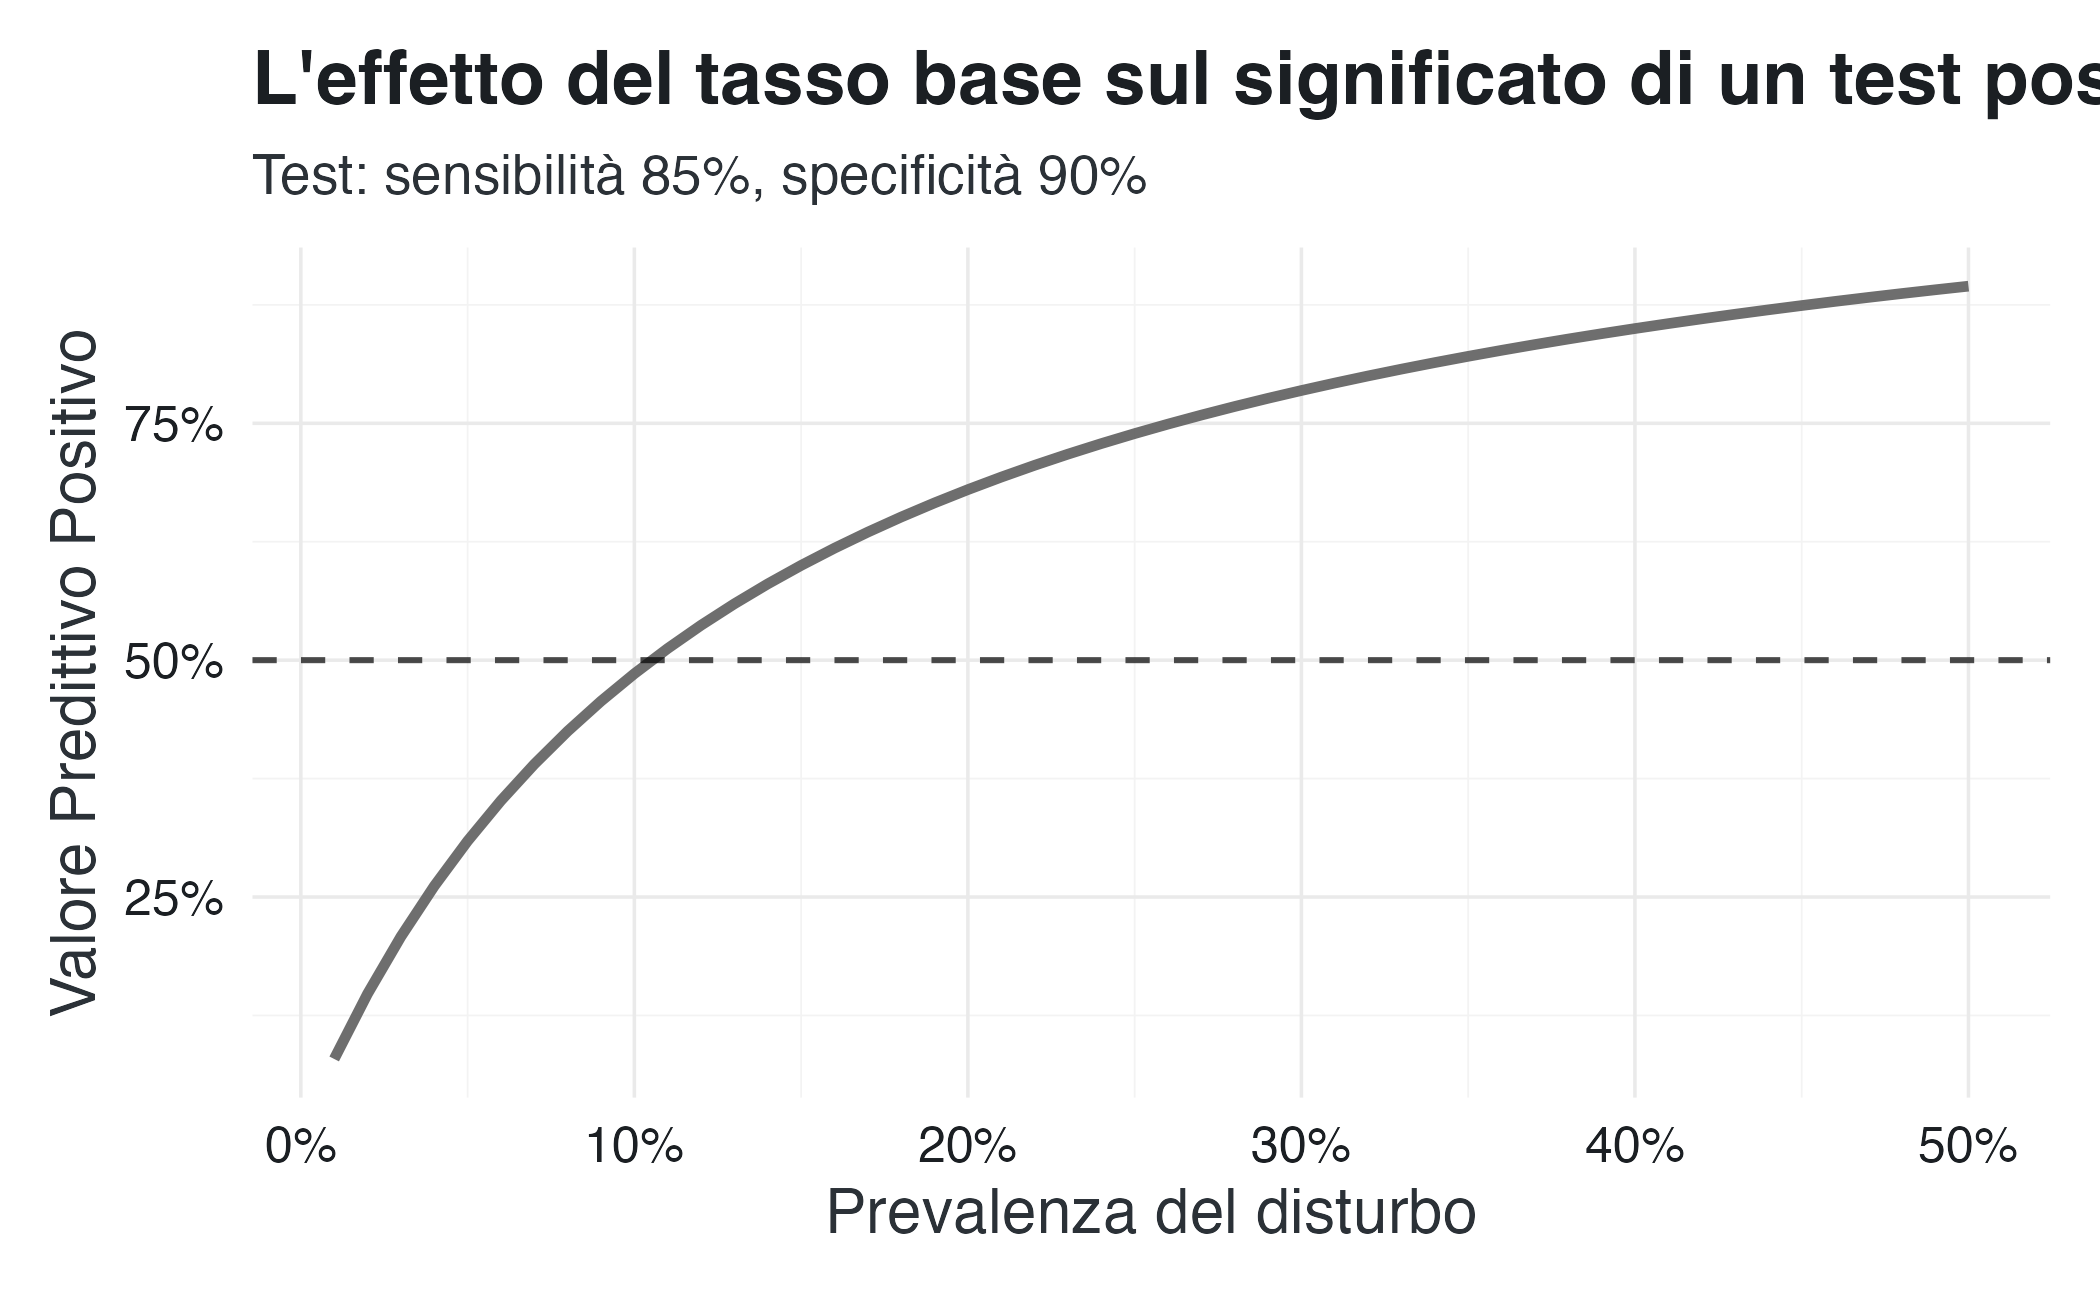
\includegraphics[width=0.85\linewidth,height=\textheight,keepaspectratio]{chapters/probability/05_bayes_theorem_files/figure-pdf/fig-base-rate-1.png}

}

\caption{\label{fig-base-rate}L'effetto della prevalenza sul valore
predittivo positivo. Lo stesso test produce interpretazioni radicalmente
diverse a seconda del contesto.}

\end{figure}%

\subsection{La lezione per la pratica}\label{la-lezione-per-la-pratica}

Il grafico illustra un principio fondamentale: \textbf{lo stesso test
può avere significati diversi in contesti diversi}.

\begin{itemize}
\tightlist
\item
  In medicina generale (prevalenza \textasciitilde8\%): un test positivo
  indica solo \textasciitilde43\% di probabilità.
\item
  In un ambulatorio specialistico (prevalenza \textasciitilde30\%): lo
  stesso test positivo indica \textasciitilde78\% di probabilità.
\end{itemize}

La differenza non sta nel test, ma nel contesto. Il teorema di Bayes ci
obbliga a considerare esplicitamente questo contesto.

\section{Applicazioni al ragionamento
clinico}\label{sec-clinical-applications}

Il teorema di Bayes non è solo uno strumento di calcolo, ma un modo di
\emph{pensare} al ragionamento clinico.

\begin{tcolorbox}[enhanced jigsaw, arc=.35mm, bottomrule=.15mm, bottomtitle=1mm, breakable, colback=white, colbacktitle=quarto-callout-note-color!10!white, colframe=quarto-callout-note-color-frame, coltitle=black, left=2mm, leftrule=.75mm, opacityback=0, opacitybacktitle=0.6, rightrule=.15mm, title=\textcolor{quarto-callout-note-color}{\faInfo}\hspace{0.5em}{Esempio: diagnostica sequenziale nell'ADHD}, titlerule=0mm, toprule=.15mm, toptitle=1mm]

Valutazione di un bambino per possibile ADHD utilizzando due strumenti
complementari.

\begin{Shaded}
\begin{Highlighting}[]
\CommentTok{\# Parametri iniziali}
\NormalTok{P\_ADHD }\OtherTok{\textless{}{-}} \FloatTok{0.05}       \CommentTok{\# Prevalenza}
\NormalTok{sens\_T1 }\OtherTok{\textless{}{-}} \FloatTok{0.80}
\NormalTok{spec\_T1 }\OtherTok{\textless{}{-}} \FloatTok{0.85}
\NormalTok{sens\_T2 }\OtherTok{\textless{}{-}} \FloatTok{0.75}
\NormalTok{spec\_T2 }\OtherTok{\textless{}{-}} \FloatTok{0.88}

\NormalTok{LR\_pos\_T1 }\OtherTok{\textless{}{-}}\NormalTok{ sens\_T1 }\SpecialCharTok{/}\NormalTok{ (}\DecValTok{1} \SpecialCharTok{{-}}\NormalTok{ spec\_T1)}
\NormalTok{LR\_pos\_T2 }\OtherTok{\textless{}{-}}\NormalTok{ sens\_T2 }\SpecialCharTok{/}\NormalTok{ (}\DecValTok{1} \SpecialCharTok{{-}}\NormalTok{ spec\_T2)}

\CommentTok{\# Aggiornamento sequenziale}
\NormalTok{prior\_odds }\OtherTok{\textless{}{-}}\NormalTok{ P\_ADHD }\SpecialCharTok{/}\NormalTok{ (}\DecValTok{1} \SpecialCharTok{{-}}\NormalTok{ P\_ADHD)}
\NormalTok{post\_odds\_T1 }\OtherTok{\textless{}{-}}\NormalTok{ prior\_odds }\SpecialCharTok{*}\NormalTok{ LR\_pos\_T1}
\NormalTok{post\_prob\_T1 }\OtherTok{\textless{}{-}}\NormalTok{ post\_odds\_T1 }\SpecialCharTok{/}\NormalTok{ (}\DecValTok{1} \SpecialCharTok{+}\NormalTok{ post\_odds\_T1)}
\NormalTok{post\_odds\_both }\OtherTok{\textless{}{-}}\NormalTok{ post\_odds\_T1 }\SpecialCharTok{*}\NormalTok{ LR\_pos\_T2}
\NormalTok{post\_prob\_both }\OtherTok{\textless{}{-}}\NormalTok{ post\_odds\_both }\SpecialCharTok{/}\NormalTok{ (}\DecValTok{1} \SpecialCharTok{+}\NormalTok{ post\_odds\_both)}

\FunctionTok{data.frame}\NormalTok{(}
  \AttributeTok{Fase =} \FunctionTok{c}\NormalTok{(}\StringTok{"Prevalenza iniziale"}\NormalTok{, }
           \StringTok{"Dopo questionario (+)"}\NormalTok{, }
           \StringTok{"Dopo osservazione (+)"}\NormalTok{),}
\NormalTok{  Probabilità }\OtherTok{=} \FunctionTok{paste0}\NormalTok{(}\FunctionTok{round}\NormalTok{(}\FunctionTok{c}\NormalTok{(P\_ADHD, post\_prob\_T1, post\_prob\_both) }\SpecialCharTok{*} \DecValTok{100}\NormalTok{, }\DecValTok{1}\NormalTok{), }\StringTok{"\%"}\NormalTok{)}
\NormalTok{)}
\CommentTok{\#\textgreater{}                    Fase Probabilità}
\CommentTok{\#\textgreater{} 1   Prevalenza iniziale          5\%}
\CommentTok{\#\textgreater{} 2 Dopo questionario (+)       21.9\%}
\CommentTok{\#\textgreater{} 3 Dopo osservazione (+)       63.7\%}
\end{Highlighting}
\end{Shaded}

\begin{Shaded}
\begin{Highlighting}[]
\NormalTok{df\_seq }\OtherTok{\textless{}{-}} \FunctionTok{data.frame}\NormalTok{(}
  \AttributeTok{Fase =} \FunctionTok{factor}\NormalTok{(}\FunctionTok{c}\NormalTok{(}\StringTok{"Prior"}\NormalTok{, }\StringTok{"Dopo T1 (+)"}\NormalTok{, }\StringTok{"Dopo T1 e T2 (+)"}\NormalTok{),}
                \AttributeTok{levels =} \FunctionTok{c}\NormalTok{(}\StringTok{"Prior"}\NormalTok{, }\StringTok{"Dopo T1 (+)"}\NormalTok{, }\StringTok{"Dopo T1 e T2 (+)"}\NormalTok{)),}
\NormalTok{  Probabilità }\OtherTok{=} \FunctionTok{c}\NormalTok{(P\_ADHD, post\_prob\_T1, post\_prob\_both)}
\NormalTok{)}

\FunctionTok{ggplot}\NormalTok{(df\_seq, }\FunctionTok{aes}\NormalTok{(}\AttributeTok{x =}\NormalTok{ Fase, }\AttributeTok{y =}\NormalTok{ Probabilità)) }\SpecialCharTok{+}
  \FunctionTok{geom\_col}\NormalTok{(}\AttributeTok{fill =} \StringTok{"\#4E79A7"}\NormalTok{, }\AttributeTok{alpha =} \FloatTok{0.8}\NormalTok{, }\AttributeTok{width =} \FloatTok{0.6}\NormalTok{) }\SpecialCharTok{+}
  \FunctionTok{geom\_text}\NormalTok{(}\FunctionTok{aes}\NormalTok{(}\AttributeTok{label =} \FunctionTok{sprintf}\NormalTok{(}\StringTok{"\%.1f\%\%"}\NormalTok{, Probabilità }\SpecialCharTok{*} \DecValTok{100}\NormalTok{)), }
            \AttributeTok{vjust =} \SpecialCharTok{{-}}\FloatTok{0.5}\NormalTok{, }\AttributeTok{size =} \FloatTok{4.5}\NormalTok{) }\SpecialCharTok{+}
  \FunctionTok{geom\_line}\NormalTok{(}\FunctionTok{aes}\NormalTok{(}\AttributeTok{group =} \DecValTok{1}\NormalTok{), }\AttributeTok{linewidth =} \DecValTok{1}\NormalTok{, }\AttributeTok{alpha =} \FloatTok{0.6}\NormalTok{) }\SpecialCharTok{+}
  \FunctionTok{geom\_point}\NormalTok{(}\AttributeTok{size =} \DecValTok{3}\NormalTok{) }\SpecialCharTok{+}
  \FunctionTok{scale\_y\_continuous}\NormalTok{(}\AttributeTok{labels =}\NormalTok{ scales}\SpecialCharTok{::}\NormalTok{percent, }\AttributeTok{limits =} \FunctionTok{c}\NormalTok{(}\DecValTok{0}\NormalTok{, }\FloatTok{0.75}\NormalTok{)) }\SpecialCharTok{+}
  \FunctionTok{labs}\NormalTok{(}
    \AttributeTok{title =} \StringTok{"Aggiornamento bayesiano sequenziale"}\NormalTok{,}
    \AttributeTok{subtitle =} \FunctionTok{paste0}\NormalTok{(}\StringTok{"LR+ T1 = "}\NormalTok{, }\FunctionTok{round}\NormalTok{(LR\_pos\_T1, }\DecValTok{1}\NormalTok{), }
                     \StringTok{", LR+ T2 = "}\NormalTok{, }\FunctionTok{round}\NormalTok{(LR\_pos\_T2, }\DecValTok{1}\NormalTok{)),}
    \AttributeTok{y =} \StringTok{"P(ADHD)"}
\NormalTok{  )}
\end{Highlighting}
\end{Shaded}

\begin{figure}[H]

\centering{

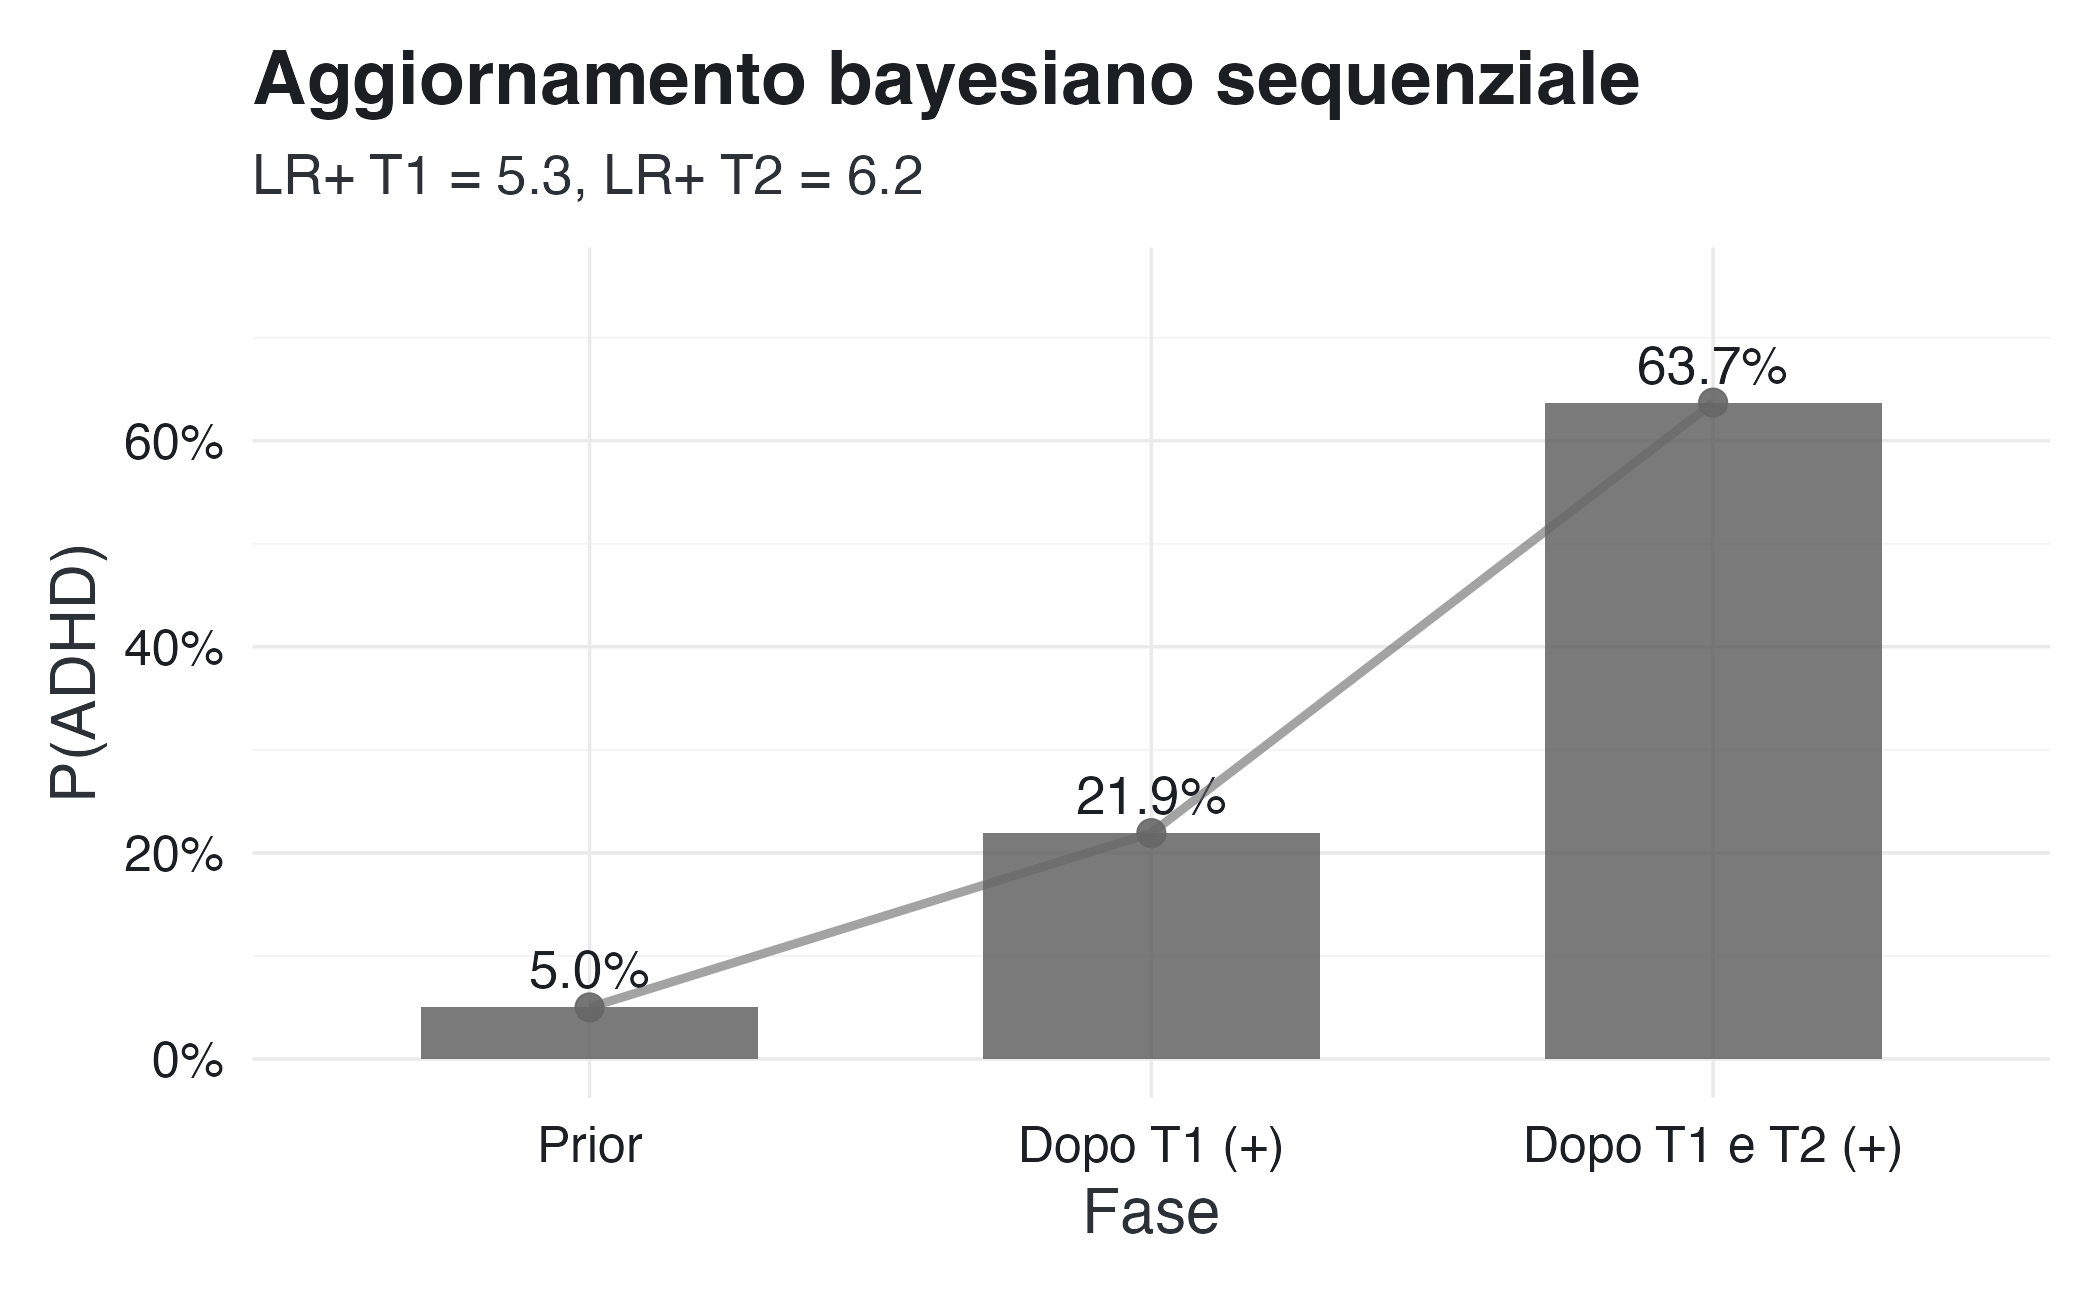
\includegraphics[width=0.85\linewidth,height=\textheight,keepaspectratio]{chapters/probability/05_bayes_theorem_files/figure-pdf/fig-sequential-adhd-1.png}

}

\caption{\label{fig-sequential-adhd}L'accumulo bayesiano di evidenze:
ogni test positivo incrementa la probabilità.}

\end{figure}%

\textbf{Principi illustrati}:

\begin{enumerate}
\def\labelenumi{\arabic{enumi}.}
\tightlist
\item
  L'evidenza si accumula: dal 5\% al 64\% dopo due test positivi.
\item
  I rapporti di verosimiglianza si moltiplicano.
\item
  Il prior conta: la stessa evidenza produrrebbe conclusioni diverse con
  un prior diverso.
\end{enumerate}

\end{tcolorbox}

\section{Come interpretare il risultato di un test
psicologico}\label{sec-interpreting-test-results}

Abbiamo discusso il teorema di Bayes attraverso esempi diagnostici. Ma
cosa significa questo \emph{concretamente} per uno psicologo che
somministra un test a un paziente?

\subsection{Lo scenario}\label{lo-scenario}

Immaginate di aver somministrato il Beck Depression Inventory (BDI-II) a
un paziente. Il punteggio è 22, che supera il cut-off clinico. Cosa
potete concludere?

La risposta \emph{non} è: ``Il paziente è depresso.'' E nemmeno: ``C'è
il 90\% di probabilità che il paziente sia depresso.''

\subsection{L'errore da evitare}\label{lerrore-da-evitare}

Confondere \(P(T^+ \mid D)\) con \(P(D \mid T^+)\). La sensibilità ci
dice quanto è probabile che il test sia positivo \emph{se} il paziente è
depresso. Noi vogliamo sapere quanto è probabile che il paziente sia
depresso \emph{dato che} il test è positivo.

\subsection{L'interpretazione corretta}\label{linterpretazione-corretta}

\textbf{1. La probabilità pre-test (il prior)}

Prima del test, avevate già informazioni sul paziente. Se il paziente si
presenta con sintomi di depressione da tre mesi, la probabilità pre-test
era già alta (60-70\%). Se il test è uno screening di routine, la
probabilità pre-test era bassa (5-10\%).

\textbf{2. L'evidenza fornita dal test (la verosimiglianza)}

Il test positivo modifica la credenza iniziale. Un test con alta
sensibilità e specificità fornisce un'evidenza forte.

\textbf{3. La probabilità post-test (il posterior)}

È la sintesi bayesiana di prior ed evidenza.

\subsection{Esempio numerico}\label{esempio-numerico}

Supponiamo che il BDI-II abbia sensibilità 0.85 e specificità 0.80.

\begin{Shaded}
\begin{Highlighting}[]
\NormalTok{sens }\OtherTok{\textless{}{-}} \FloatTok{0.85}
\NormalTok{spec }\OtherTok{\textless{}{-}} \FloatTok{0.80}
\NormalTok{LR\_pos }\OtherTok{\textless{}{-}}\NormalTok{ sens }\SpecialCharTok{/}\NormalTok{ (}\DecValTok{1} \SpecialCharTok{{-}}\NormalTok{ spec)  }\CommentTok{\# = 4.25}

\CommentTok{\# Due scenari}
\NormalTok{prior\_sintomatico }\OtherTok{\textless{}{-}} \FloatTok{0.65}
\NormalTok{prior\_screening }\OtherTok{\textless{}{-}} \FloatTok{0.08}

\NormalTok{calcola\_posterior }\OtherTok{\textless{}{-}} \ControlFlowTok{function}\NormalTok{(prior, LR) \{}
\NormalTok{  odds\_prior }\OtherTok{\textless{}{-}}\NormalTok{ prior }\SpecialCharTok{/}\NormalTok{ (}\DecValTok{1} \SpecialCharTok{{-}}\NormalTok{ prior)}
\NormalTok{  odds\_post }\OtherTok{\textless{}{-}}\NormalTok{ odds\_prior }\SpecialCharTok{*}\NormalTok{ LR}
\NormalTok{  odds\_post }\SpecialCharTok{/}\NormalTok{ (}\DecValTok{1} \SpecialCharTok{+}\NormalTok{ odds\_post)}
\NormalTok{\}}

\NormalTok{post\_sintomatico }\OtherTok{\textless{}{-}} \FunctionTok{calcola\_posterior}\NormalTok{(prior\_sintomatico, LR\_pos)}
\NormalTok{post\_screening }\OtherTok{\textless{}{-}} \FunctionTok{calcola\_posterior}\NormalTok{(prior\_screening, LR\_pos)}

\FunctionTok{cat}\NormalTok{(}\StringTok{"Paziente sintomatico: da"}\NormalTok{, prior\_sintomatico}\SpecialCharTok{*}\DecValTok{100}\NormalTok{, }\StringTok{"\% a"}\NormalTok{, }
    \FunctionTok{round}\NormalTok{(post\_sintomatico}\SpecialCharTok{*}\DecValTok{100}\NormalTok{, }\DecValTok{1}\NormalTok{), }\StringTok{"\%}\SpecialCharTok{\textbackslash{}n}\StringTok{"}\NormalTok{)}
\CommentTok{\#\textgreater{} Paziente sintomatico: da 65 \% a 88.8 \%}
\FunctionTok{cat}\NormalTok{(}\StringTok{"Screening aziendale: da"}\NormalTok{, prior\_screening}\SpecialCharTok{*}\DecValTok{100}\NormalTok{, }\StringTok{"\% a"}\NormalTok{, }
    \FunctionTok{round}\NormalTok{(post\_screening}\SpecialCharTok{*}\DecValTok{100}\NormalTok{, }\DecValTok{1}\NormalTok{), }\StringTok{"\%}\SpecialCharTok{\textbackslash{}n}\StringTok{"}\NormalTok{)}
\CommentTok{\#\textgreater{} Screening aziendale: da 8 \% a 27 \%}
\end{Highlighting}
\end{Shaded}

Lo stesso test positivo porta a conclusioni diverse: 88\% di probabilità
per il paziente sintomatico, solo 27\% per il dipendente in screening.

\subsection{Il messaggio per la
pratica}\label{il-messaggio-per-la-pratica}

\textbf{Un test non vi dice se il paziente ha una determinata
condizione. Vi dice quanto dovreste aggiornare la vostra credenza, sulla
base della vostra valutazione iniziale.} Questa distinzione ha
conseguenze profonde per la qualità del ragionamento clinico.

\section{Aggiornamento bayesiano con distribuzioni
continue}\label{sec-bayes-continuous}

Quando il parametro di interesse è continuo, l'aggiornamento bayesiano
opera su \emph{distribuzioni di probabilità}.

\subsection{Il modello Beta-Binomiale}\label{il-modello-beta-binomiale}

Quando \(\theta \in [0,1]\) e i dati sono binari, la distribuzione
\textbf{Beta} offre un framework elegante:

\begin{tcolorbox}[enhanced jigsaw, arc=.35mm, bottomrule=.15mm, bottomtitle=1mm, breakable, colback=white, colbacktitle=quarto-callout-important-color!10!white, colframe=quarto-callout-important-color-frame, coltitle=black, left=2mm, leftrule=.75mm, opacityback=0, opacitybacktitle=0.6, rightrule=.15mm, title=\textcolor{quarto-callout-important-color}{\faExclamation}\hspace{0.5em}{Coniugazione Beta-Binomiale}, titlerule=0mm, toprule=.15mm, toptitle=1mm]

\begin{itemize}
\tightlist
\item
  \textbf{Prior}: \(\theta \sim \text{Beta}(\alpha, \beta)\).
\item
  \textbf{Dati}: \(k\) successi su \(n\) prove.
\item
  \textbf{Posterior}:
  \(\theta \mid k \sim \text{Beta}(\alpha + k, \beta + n - k)\).
\end{itemize}

\end{tcolorbox}

\subsection{Esempio: valutazione di uno
studente}\label{esempio-valutazione-di-uno-studente}

Consideriamo un test a scelta multipla con 4 opzioni. Prior:
\(\text{Beta}(1,3)\), che riflette l'ipotesi di risposta casuale (media
= 0.25). Osserviamo 12 risposte corrette su 30.

\begin{Shaded}
\begin{Highlighting}[]
\NormalTok{alpha\_prior }\OtherTok{\textless{}{-}} \DecValTok{1}
\NormalTok{beta\_prior }\OtherTok{\textless{}{-}} \DecValTok{3}
\NormalTok{n\_obs }\OtherTok{\textless{}{-}} \DecValTok{30}
\NormalTok{k\_success }\OtherTok{\textless{}{-}} \DecValTok{12}

\NormalTok{alpha\_post }\OtherTok{\textless{}{-}}\NormalTok{ alpha\_prior }\SpecialCharTok{+}\NormalTok{ k\_success}
\NormalTok{beta\_post }\OtherTok{\textless{}{-}}\NormalTok{ beta\_prior }\SpecialCharTok{+}\NormalTok{ (n\_obs }\SpecialCharTok{{-}}\NormalTok{ k\_success)}

\NormalTok{theta\_seq }\OtherTok{\textless{}{-}} \FunctionTok{seq}\NormalTok{(}\DecValTok{0}\NormalTok{, }\DecValTok{1}\NormalTok{, }\AttributeTok{length.out =} \DecValTok{500}\NormalTok{)}
\NormalTok{prior\_dens }\OtherTok{\textless{}{-}} \FunctionTok{dbeta}\NormalTok{(theta\_seq, alpha\_prior, beta\_prior)}
\NormalTok{posterior\_dens }\OtherTok{\textless{}{-}} \FunctionTok{dbeta}\NormalTok{(theta\_seq, alpha\_post, beta\_post)}

\CommentTok{\# Verosimiglianza (normalizzata per visualizzazione)}
\NormalTok{lik\_dens }\OtherTok{\textless{}{-}} \FunctionTok{dbinom}\NormalTok{(k\_success, n\_obs, theta\_seq)}
\NormalTok{lik\_dens }\OtherTok{\textless{}{-}}\NormalTok{ lik\_dens }\SpecialCharTok{/} \FunctionTok{max}\NormalTok{(lik\_dens) }\SpecialCharTok{*} \FunctionTok{max}\NormalTok{(posterior\_dens)}

\NormalTok{df\_beta }\OtherTok{\textless{}{-}} \FunctionTok{data.frame}\NormalTok{(}
  \AttributeTok{theta =} \FunctionTok{rep}\NormalTok{(theta\_seq, }\DecValTok{3}\NormalTok{),}
\NormalTok{  Densità }\OtherTok{=} \FunctionTok{c}\NormalTok{(prior\_dens, lik\_dens, posterior\_dens),}
  \AttributeTok{Componente =} \FunctionTok{rep}\NormalTok{(}\FunctionTok{c}\NormalTok{(}\StringTok{"Prior"}\NormalTok{, }\StringTok{"Verosimiglianza"}\NormalTok{, }\StringTok{"Posterior"}\NormalTok{), }\AttributeTok{each =} \DecValTok{500}\NormalTok{)}
\NormalTok{)}

\FunctionTok{ggplot}\NormalTok{(df\_beta, }\FunctionTok{aes}\NormalTok{(}\AttributeTok{x =}\NormalTok{ theta, }\AttributeTok{y =}\NormalTok{ Densità, }\AttributeTok{color =}\NormalTok{ Componente, }\AttributeTok{linetype =}\NormalTok{ Componente)) }\SpecialCharTok{+}
  \FunctionTok{geom\_line}\NormalTok{(}\AttributeTok{linewidth =} \FloatTok{1.2}\NormalTok{) }\SpecialCharTok{+}
  \FunctionTok{geom\_vline}\NormalTok{(}\AttributeTok{xintercept =} \FloatTok{0.25}\NormalTok{, }\AttributeTok{linetype =} \StringTok{"dotted"}\NormalTok{, }\AttributeTok{alpha =} \FloatTok{0.5}\NormalTok{) }\SpecialCharTok{+}
  \FunctionTok{geom\_vline}\NormalTok{(}\AttributeTok{xintercept =}\NormalTok{ k\_success}\SpecialCharTok{/}\NormalTok{n\_obs, }\AttributeTok{linetype =} \StringTok{"dotted"}\NormalTok{, }\AttributeTok{alpha =} \FloatTok{0.5}\NormalTok{) }\SpecialCharTok{+}
  \FunctionTok{scale\_linetype\_manual}\NormalTok{(}\AttributeTok{values =} \FunctionTok{c}\NormalTok{(}\StringTok{"Prior"} \OtherTok{=} \StringTok{"dashed"}\NormalTok{, }
                                   \StringTok{"Verosimiglianza"} \OtherTok{=} \StringTok{"dotted"}\NormalTok{, }
                                   \StringTok{"Posterior"} \OtherTok{=} \StringTok{"solid"}\NormalTok{)) }\SpecialCharTok{+}
  \FunctionTok{labs}\NormalTok{(}
    \AttributeTok{title =} \StringTok{"Aggiornamento bayesiano: 12 corrette su 30 domande"}\NormalTok{,}
    \AttributeTok{x =} \FunctionTok{expression}\NormalTok{(theta }\SpecialCharTok{\textasciitilde{}} \StringTok{"(probabilità di risposta corretta)"}\NormalTok{),}
    \AttributeTok{y =} \StringTok{"Densità"}
\NormalTok{  )}
\end{Highlighting}
\end{Shaded}

\begin{figure}[H]

\centering{

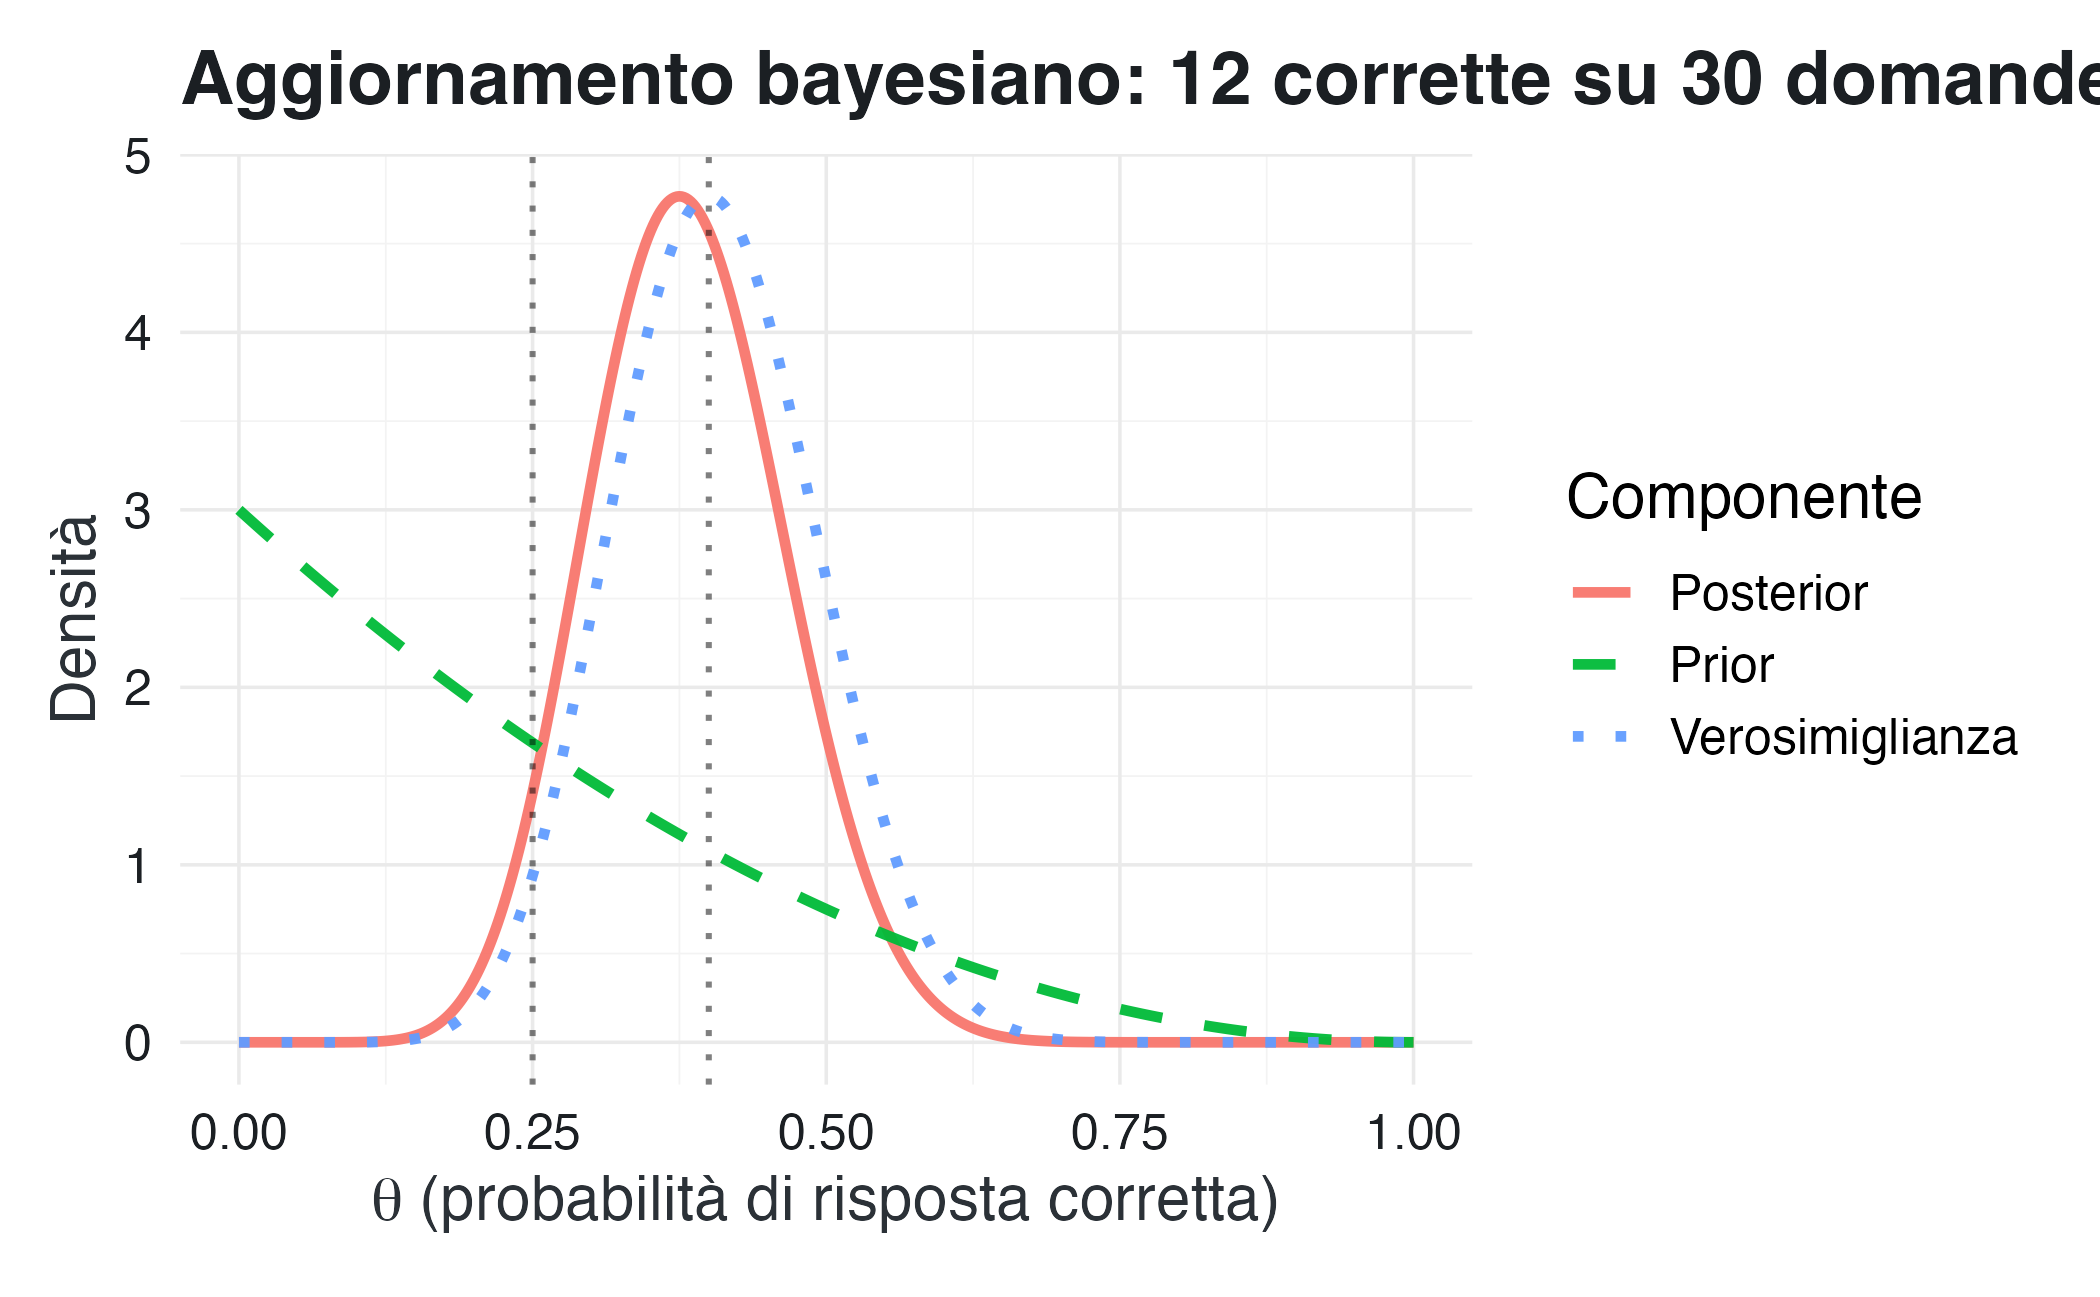
\includegraphics[width=0.85\linewidth,height=\textheight,keepaspectratio]{chapters/probability/05_bayes_theorem_files/figure-pdf/fig-beta-update-1.png}

}

\caption{\label{fig-beta-update}L'aggiornamento bayesiano nel modello
Beta-Binomiale: il posterior è un compromesso tra prior e
verosimiglianza.}

\end{figure}%

Il posterior è un \emph{compromesso} tra prior e dati. La media a
posteriori si colloca tra il prior (0.25) e i dati (0.40).

\subsection{Intervalli di
credibilità}\label{intervalli-di-credibilituxe0}

A differenza degli intervalli di confidenza, gli intervalli di
credibilità bayesiani forniscono affermazioni dirette sulla probabilità
che il parametro cada in un certo intervallo.

\begin{Shaded}
\begin{Highlighting}[]
\NormalTok{ci\_lower }\OtherTok{\textless{}{-}} \FunctionTok{qbeta}\NormalTok{(}\FloatTok{0.025}\NormalTok{, alpha\_post, beta\_post)}
\NormalTok{ci\_upper }\OtherTok{\textless{}{-}} \FunctionTok{qbeta}\NormalTok{(}\FloatTok{0.975}\NormalTok{, alpha\_post, beta\_post)}

\NormalTok{df\_post }\OtherTok{\textless{}{-}} \FunctionTok{data.frame}\NormalTok{(}\AttributeTok{theta =}\NormalTok{ theta\_seq, densità }\OtherTok{=}\NormalTok{ posterior\_dens)}

\FunctionTok{ggplot}\NormalTok{(df\_post, }\FunctionTok{aes}\NormalTok{(}\AttributeTok{x =}\NormalTok{ theta, }\AttributeTok{y =}\NormalTok{ densità)) }\SpecialCharTok{+}
  \FunctionTok{geom\_line}\NormalTok{(}\AttributeTok{linewidth =} \FloatTok{1.2}\NormalTok{) }\SpecialCharTok{+}
  \FunctionTok{geom\_area}\NormalTok{(}\AttributeTok{data =}\NormalTok{ df\_post }\SpecialCharTok{\%\textgreater{}\%} \FunctionTok{filter}\NormalTok{(theta }\SpecialCharTok{\textgreater{}=}\NormalTok{ ci\_lower }\SpecialCharTok{\&}\NormalTok{ theta }\SpecialCharTok{\textless{}=}\NormalTok{ ci\_upper),}
            \AttributeTok{alpha =} \FloatTok{0.3}\NormalTok{) }\SpecialCharTok{+}
  \FunctionTok{geom\_vline}\NormalTok{(}\AttributeTok{xintercept =} \FunctionTok{c}\NormalTok{(ci\_lower, ci\_upper), }\AttributeTok{linetype =} \StringTok{"dashed"}\NormalTok{) }\SpecialCharTok{+}
  \FunctionTok{geom\_vline}\NormalTok{(}\AttributeTok{xintercept =}\NormalTok{ alpha\_post}\SpecialCharTok{/}\NormalTok{(alpha\_post }\SpecialCharTok{+}\NormalTok{ beta\_post), }\AttributeTok{linewidth =} \DecValTok{1}\NormalTok{) }\SpecialCharTok{+}
  \FunctionTok{annotate}\NormalTok{(}\StringTok{"text"}\NormalTok{, }\AttributeTok{x =}\NormalTok{ (ci\_lower }\SpecialCharTok{+}\NormalTok{ ci\_upper)}\SpecialCharTok{/}\DecValTok{2}\NormalTok{, }\AttributeTok{y =} \FunctionTok{max}\NormalTok{(posterior\_dens) }\SpecialCharTok{*} \FloatTok{0.4}\NormalTok{,}
           \AttributeTok{label =} \FunctionTok{paste0}\NormalTok{(}\StringTok{"IC 95\%}\SpecialCharTok{\textbackslash{}n}\StringTok{["}\NormalTok{, }\FunctionTok{round}\NormalTok{(ci\_lower, }\DecValTok{2}\NormalTok{), }\StringTok{", "}\NormalTok{, }\FunctionTok{round}\NormalTok{(ci\_upper, }\DecValTok{2}\NormalTok{), }\StringTok{"]"}\NormalTok{)) }\SpecialCharTok{+}
  \FunctionTok{labs}\NormalTok{(}
    \AttributeTok{title =} \StringTok{"Quantificazione dell\textquotesingle{}incertezza su θ"}\NormalTok{,}
    \AttributeTok{x =} \FunctionTok{expression}\NormalTok{(theta),}
    \AttributeTok{y =} \StringTok{"Densità a posteriori"}
\NormalTok{  )}
\end{Highlighting}
\end{Shaded}

\begin{figure}[H]

\centering{

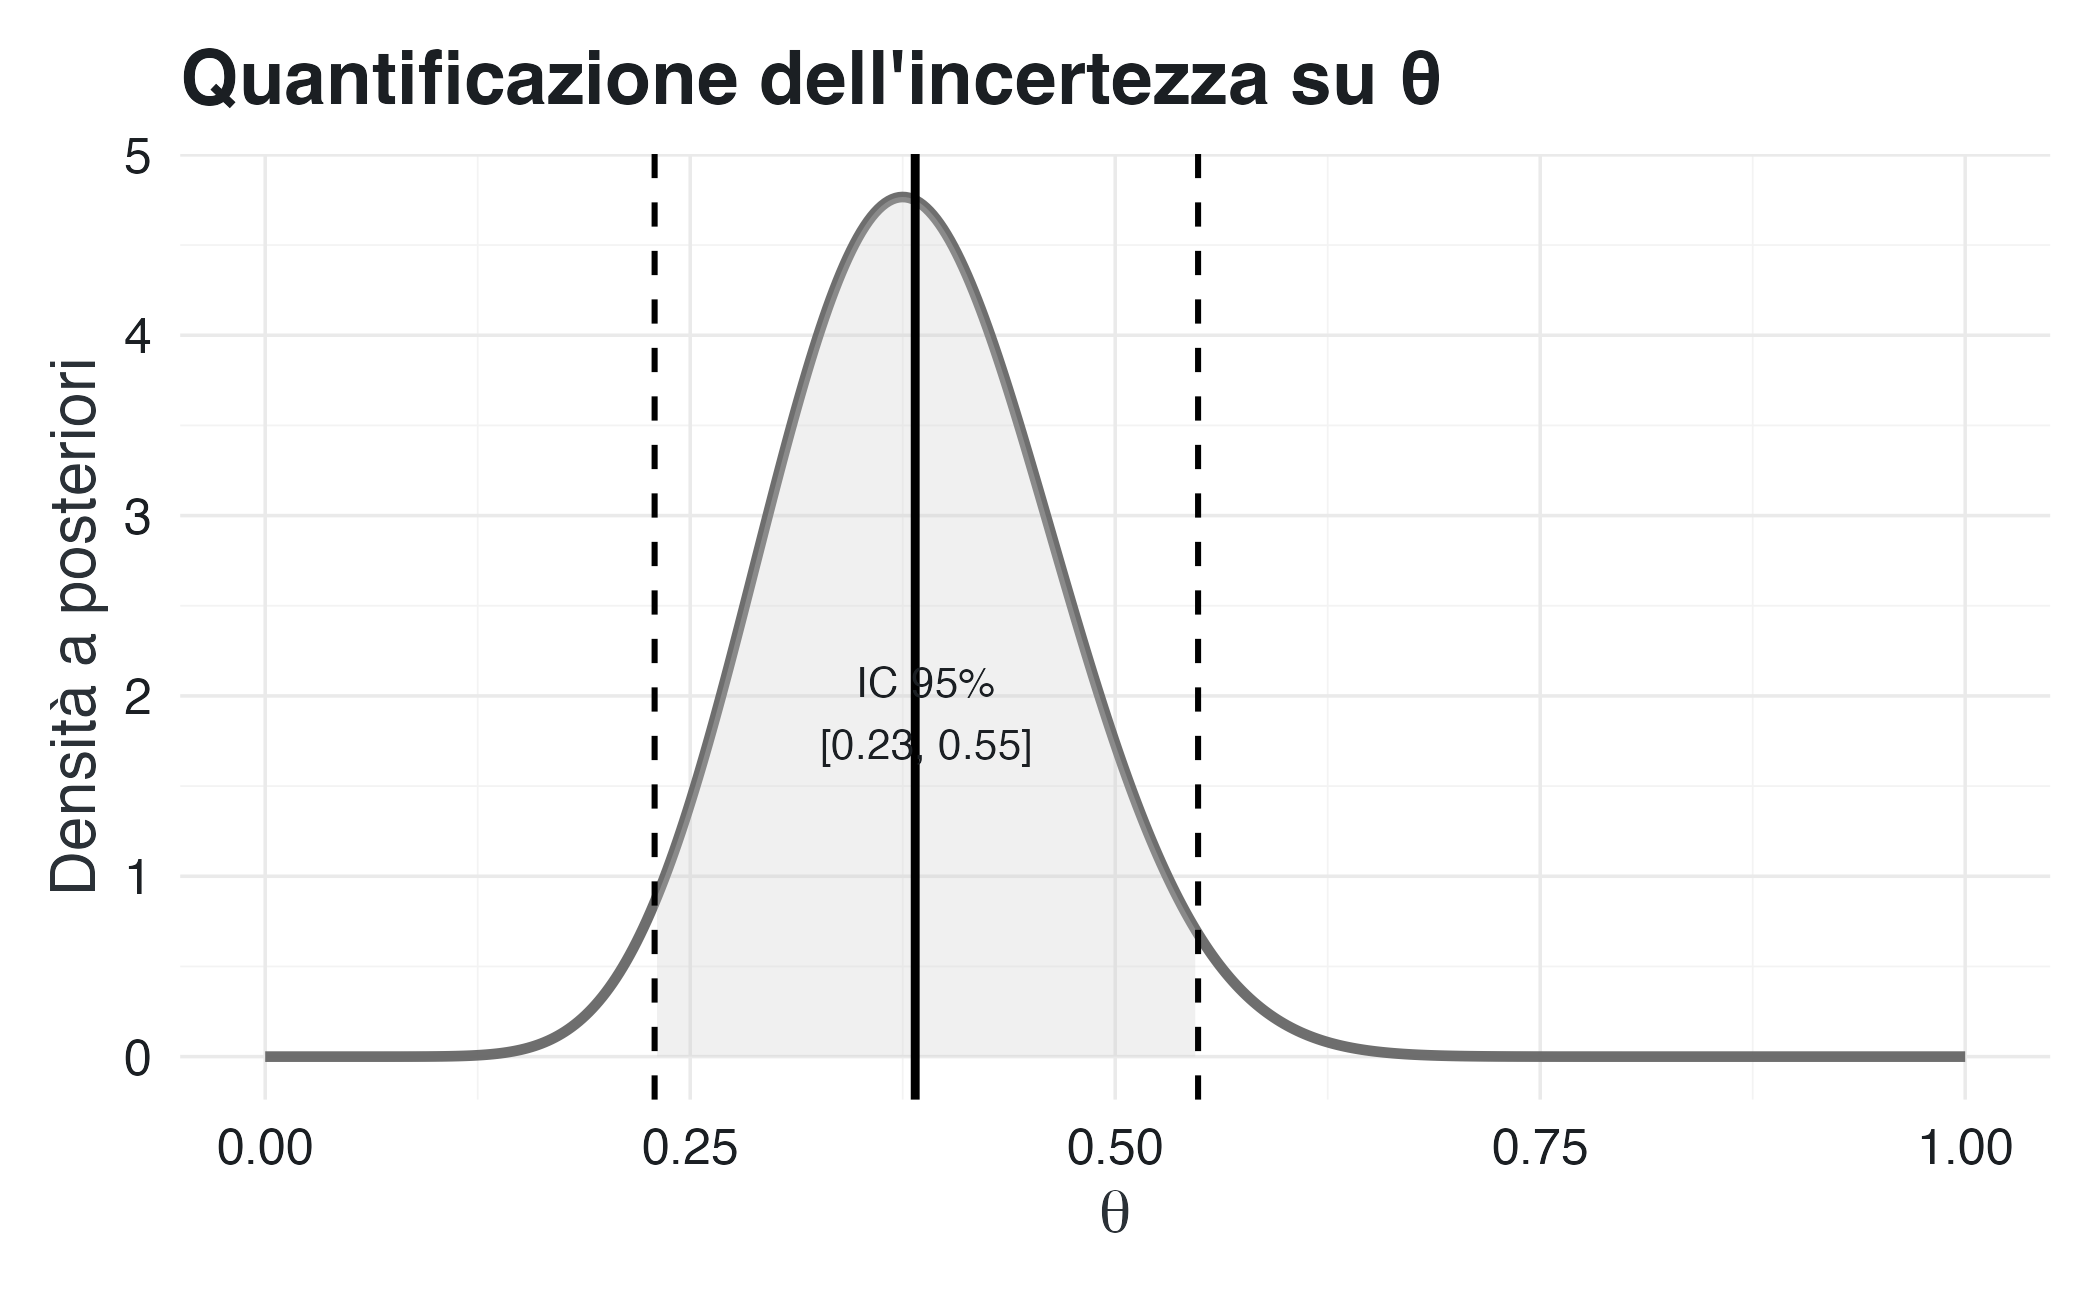
\includegraphics[width=0.85\linewidth,height=\textheight,keepaspectratio]{chapters/probability/05_bayes_theorem_files/figure-pdf/fig-credible-interval-1.png}

}

\caption{\label{fig-credible-interval}Distribuzione a posteriori con
intervallo di credibilità al 95\%.}

\end{figure}%

\begin{tcolorbox}[enhanced jigsaw, arc=.35mm, bottomrule=.15mm, bottomtitle=1mm, breakable, colback=white, colbacktitle=quarto-callout-important-color!10!white, colframe=quarto-callout-important-color-frame, coltitle=black, left=2mm, leftrule=.75mm, opacityback=0, opacitybacktitle=0.6, rightrule=.15mm, title=\textcolor{quarto-callout-important-color}{\faExclamation}\hspace{0.5em}{Interpretazione degli intervalli di credibilità}, titlerule=0mm, toprule=.15mm, toptitle=1mm]

\textbf{Intervallo di credibilità bayesiano (95\%)}: ``C'è una
probabilità del 95\% che il vero valore del parametro sia compreso tra
0.23 e 0.55, date le nostre informazioni.''

\textbf{Intervallo di confidenza frequentista (95\%)}: ``Se ripetessimo
questo esperimento infinite volte, il 95\% degli intervalli conterrebbe
il vero parametro.''

La prima interpretazione è diretta e intuitiva; la seconda riguarda le
proprietà della procedura.

\end{tcolorbox}

\section*{Riflessioni conclusive}\label{riflessioni-conclusive-4}

\markright{Riflessioni conclusive}

Siamo arrivati al termine del percorso che ha costruito le fondamenta
del ragionamento bayesiano. Il teorema di Bayes non è stato presentato
come una formula da memorizzare, ma come l'espressione matematica di un
principio epistemologico profondo: \textbf{l'apprendimento razionale
dall'esperienza}.

\subsection{Cosa abbiamo compreso}\label{cosa-abbiamo-compreso}

La derivazione del teorema dalla simmetria della probabilità congiunta
ha mostrato che l'aggiornamento bayesiano non è una scelta metodologica
arbitraria. È una \emph{necessità logica} per chiunque accetti i vincoli
di coerenza della teoria della probabilità.

L'interpretazione epistemica dei componenti ha rivelato una struttura
del ragionamento che è al tempo stesso rigorosa e intuitiva.

Le applicazioni diagnostiche hanno illustrato sia il potere del teorema
sia i pericoli dell'intuizione non guidata. La fallacia del tasso base è
una delle scoperte più robuste della psicologia del giudizio.

\subsection{Il messaggio fondamentale}\label{il-messaggio-fondamentale}

Se dovessimo condensare tutto in un'unica idea, sarebbe questa:
\textbf{la razionalità è coerenza, e la coerenza richiede Bayes}.

Questo non significa che l'approccio bayesiano sia l'unico valido.
Significa che, una volta accettata l'interpretazione della probabilità
come grado di credenza, l'aggiornamento bayesiano segue come conseguenza
inevitabile.

\subsection{Verso il futuro}\label{verso-il-futuro}

Questo capitolo conclude la trattazione dei fondamenti. I concetti
stabiliti --- prior, verosimiglianza, posterior, aggiornamento
sequenziale, quantificazione dell'incertezza --- costituiranno la base
per tutto ciò che seguirà.

Come scrisse Laplace oltre due secoli fa, il calcolo delle probabilità
non è altro che ``il buon senso ridotto a calcolo''. Il teorema di Bayes
è il motore che rende possibile questa riduzione.

\section*{Punti chiave da ricordare}\label{punti-chiave-da-ricordare-4}

\markright{Punti chiave da ricordare}

\begin{tcolorbox}[enhanced jigsaw, arc=.35mm, bottomrule=.15mm, bottomtitle=1mm, breakable, colback=white, colbacktitle=quarto-callout-important-color!10!white, colframe=quarto-callout-important-color-frame, coltitle=black, left=2mm, leftrule=.75mm, opacityback=0, opacitybacktitle=0.6, rightrule=.15mm, title=\textcolor{quarto-callout-important-color}{\faExclamation}\hspace{0.5em}{Importante}, titlerule=0mm, toprule=.15mm, toptitle=1mm]

\begin{enumerate}
\def\labelenumi{\arabic{enumi}.}
\tightlist
\item
  \textbf{Il teorema di Bayes come inversione probabilistica}

  \begin{itemize}
  \tightlist
  \item
    Deriva dalla simmetria della probabilità congiunta.
  \item
    Permette di passare da \(P(E \mid H)\) a \(P(H \mid E)\).
  \item
    Non è un'assunzione aggiuntiva, ma una conseguenza degli assiomi.
  \end{itemize}
\item
  \textbf{Interpretazione epistemica dei componenti}

  \begin{itemize}
  \tightlist
  \item
    \textbf{Prior} \(P(H)\): credenza prima dei dati.
  \item
    \textbf{Verosimiglianza} \(P(E \mid H)\): compatibilità
    dati-ipotesi.
  \item
    \textbf{Evidenza} \(P(E)\): normalizzazione.
  \item
    \textbf{Posterior} \(P(H \mid E)\): credenza aggiornata.
  \end{itemize}
\item
  \textbf{Forma in odds}

  \begin{itemize}
  \tightlist
  \item
    Odds posteriori = LR × Odds a priori.
  \item
    Il rapporto di verosimiglianza quantifica la forza dell'evidenza.
  \item
    Aggiornamenti sequenziali: i LR si moltiplicano.
  \end{itemize}
\item
  \textbf{La fallacia del tasso base}

  \begin{itemize}
  \tightlist
  \item
    Ignorare la prevalenza porta a sovrastimare il VPP.
  \item
    Lo stesso test ha significati diversi in contesti diversi.
  \item
    Il teorema di Bayes costringe a considerare il contesto.
  \end{itemize}
\item
  \textbf{Aggiornamento con distribuzioni continue}

  \begin{itemize}
  \tightlist
  \item
    Beta-Binomiale:
    \(\text{Beta}(\alpha, \beta) \to \text{Beta}(\alpha+k, \beta+n-k)\).
  \item
    Intervalli di credibilità: interpretazione probabilistica diretta.
  \end{itemize}
\end{enumerate}

\textbf{Formule da ricordare:}

\[P(H \mid E) = \frac{P(E \mid H) \cdot P(H)}{P(E)}\]

\[\text{Odds}(H \mid E) = \text{LR} \times \text{Odds}(H)\]

\[\text{LR}^+ = \frac{\text{Sensibilità}}{1 - \text{Specificità}}\]

\textbf{Per il prossimo capitolo:}

Nel Capitolo~\ref{sec-prob-random-var} inizieremo lo studio delle
\textbf{variabili casuali}, formalizzando il passaggio da eventi
discreti a quantità numeriche.

\end{tcolorbox}

\begin{tcolorbox}[enhanced jigsaw, arc=.35mm, bottomrule=.15mm, bottomtitle=1mm, breakable, colback=white, colbacktitle=quarto-callout-note-color!10!white, colframe=quarto-callout-note-color-frame, coltitle=black, left=2mm, leftrule=.75mm, opacityback=0, opacitybacktitle=0.6, rightrule=.15mm, title=\textcolor{quarto-callout-note-color}{\faInfo}\hspace{0.5em}{Informazioni sull'ambiente di sviluppo}, titlerule=0mm, toprule=.15mm, toptitle=1mm]

\begin{Shaded}
\begin{Highlighting}[]
\FunctionTok{sessionInfo}\NormalTok{()}
\CommentTok{\#\textgreater{} R version 4.6.1 (2026{-}06{-}24)}
\CommentTok{\#\textgreater{} Platform: aarch64{-}apple{-}darwin23}
\CommentTok{\#\textgreater{} Running under: macOS Tahoe 26.5.2}
\CommentTok{\#\textgreater{} }
\CommentTok{\#\textgreater{} Matrix products: default}
\CommentTok{\#\textgreater{} BLAS:   /Library/Frameworks/R.framework/Versions/4.6/Resources/lib/libRblas.0.dylib }
\CommentTok{\#\textgreater{} LAPACK: /Library/Frameworks/R.framework/Versions/4.6/Resources/lib/libRlapack.dylib;  LAPACK version 3.12.1}
\CommentTok{\#\textgreater{} }
\CommentTok{\#\textgreater{} locale:}
\CommentTok{\#\textgreater{} [1] C.UTF{-}8/UTF{-}8/C.UTF{-}8/C/C.UTF{-}8/C.UTF{-}8}
\CommentTok{\#\textgreater{} }
\CommentTok{\#\textgreater{} time zone: Europe/Rome}
\CommentTok{\#\textgreater{} tzcode source: internal}
\CommentTok{\#\textgreater{} }
\CommentTok{\#\textgreater{} attached base packages:}
\CommentTok{\#\textgreater{} [1] stats     graphics  grDevices utils     datasets  methods   base     }
\CommentTok{\#\textgreater{} }
\CommentTok{\#\textgreater{} other attached packages:}
\CommentTok{\#\textgreater{}  [1] ragg\_1.5.2            tinytable\_0.17.0      withr\_3.0.3          }
\CommentTok{\#\textgreater{}  [4] systemfonts\_1.3.2     patchwork\_1.3.2       ggdist\_3.3.3         }
\CommentTok{\#\textgreater{}  [7] tidybayes\_3.0.7       bayesplot\_1.15.0      ggplot2\_4.0.3        }
\CommentTok{\#\textgreater{} [10] reliabilitydiag\_0.2.1 priorsense\_1.2.0      posterior\_1.7.0      }
\CommentTok{\#\textgreater{} [13] loo\_2.10.0            rstan\_2.32.7          StanHeaders\_2.32.10  }
\CommentTok{\#\textgreater{} [16] brms\_2.23.0           Rcpp\_1.1.2            sessioninfo\_1.2.4    }
\CommentTok{\#\textgreater{} [19] conflicted\_1.2.0      janitor\_2.2.1         matrixStats\_1.5.0    }
\CommentTok{\#\textgreater{} [22] modelr\_0.1.11         tibble\_3.3.1          dplyr\_1.2.1          }
\CommentTok{\#\textgreater{} [25] tidyr\_1.3.2           rio\_1.3.0             here\_1.0.2           }
\CommentTok{\#\textgreater{} }
\CommentTok{\#\textgreater{} loaded via a namespace (and not attached):}
\CommentTok{\#\textgreater{}  [1] svUnit\_1.0.8          tidyselect\_1.2.1      farver\_2.1.2         }
\CommentTok{\#\textgreater{}  [4] S7\_0.2.2              fastmap\_1.2.0         tensorA\_0.36.2.1     }
\CommentTok{\#\textgreater{}  [7] digest\_0.6.39         timechange\_0.4.0      estimability\_2.0.0   }
\CommentTok{\#\textgreater{} [10] lifecycle\_1.0.5       magrittr\_2.0.5        compiler\_4.6.1       }
\CommentTok{\#\textgreater{} [13] rlang\_1.3.0           tools\_4.6.1           yaml\_2.3.12          }
\CommentTok{\#\textgreater{} [16] knitr\_1.51            labeling\_0.4.3        bridgesampling\_1.2{-}1 }
\CommentTok{\#\textgreater{} [19] pkgbuild\_1.4.8        curl\_7.1.0            RColorBrewer\_1.1{-}3   }
\CommentTok{\#\textgreater{} [22] abind\_1.4{-}8           purrr\_1.2.2           grid\_4.6.1           }
\CommentTok{\#\textgreater{} [25] stats4\_4.6.1          xtable\_1.8{-}8          inline\_0.3.21        }
\CommentTok{\#\textgreater{} [28] emmeans\_2.0.3         scales\_1.4.0          cli\_3.6.6            }
\CommentTok{\#\textgreater{} [31] mvtnorm\_1.4{-}1         rmarkdown\_2.31        generics\_0.1.4       }
\CommentTok{\#\textgreater{} [34] otel\_0.2.0            RcppParallel\_5.1.11{-}2 cachem\_1.1.0         }
\CommentTok{\#\textgreater{} [37] stringr\_1.6.0         parallel\_4.6.1        vctrs\_0.7.3          }
\CommentTok{\#\textgreater{} [40] V8\_8.2.0              Matrix\_1.7{-}5          jsonlite\_2.0.0       }
\CommentTok{\#\textgreater{} [43] arrayhelpers\_1.1{-}1    glue\_1.8.1            codetools\_0.2{-}20     }
\CommentTok{\#\textgreater{} [46] distributional\_0.8.1  lubridate\_1.9.5       stringi\_1.8.7        }
\CommentTok{\#\textgreater{} [49] gtable\_0.3.6          QuickJSR\_1.10.0       pillar\_1.11.1        }
\CommentTok{\#\textgreater{} [52] htmltools\_0.5.9       Brobdingnag\_1.2{-}9     R6\_2.6.1             }
\CommentTok{\#\textgreater{} [55] textshaping\_1.0.5     rprojroot\_2.1.1       evaluate\_1.0.5       }
\CommentTok{\#\textgreater{} [58] lattice\_0.22{-}9        backports\_1.5.1       memoise\_2.0.1        }
\CommentTok{\#\textgreater{} [61] broom\_1.0.13          snakecase\_0.11.1      rstantools\_2.6.0     }
\CommentTok{\#\textgreater{} [64] coda\_0.19{-}4.1         gridExtra\_2.3.1       nlme\_3.1{-}169         }
\CommentTok{\#\textgreater{} [67] checkmate\_2.3.4       xfun\_0.60             pkgconfig\_2.0.3}
\end{Highlighting}
\end{Shaded}

\end{tcolorbox}

\section*{Bibliografia}\label{bibliografia-2}

\markright{Bibliografia}

\part{PARTE 2: Variabili casuali e distribuzioni}

\chapter{Variabili casuali}\label{sec-prob-random-var}

\section*{Introduzione}\label{introduzione-5}

\markright{Introduzione}

Si consideri uno scenario ricorrente nella pratica clinica in cui il
clinico intende valutare l'efficacia di un intervento per il disturbo
d'ansia sociale. A tale scopo, somministra la \emph{Liebowitz Social
Anxiety Scale} (LSAS) a un campione di 50 pazienti, rilevando le
misurazioni prima e dopo un ciclo di 12 sedute.

Il quesito metodologico non si esaurisce in una semplice dicotomia,
ovvero nel capire se l'intervento funzioni o meno, ma verte sulla stima
dell'entità attesa del miglioramento, sulla distribuzione di probabilità
che caratterizza i potenziali effetti e sulla misura di incertezza da
associare a tali stime.

Per rispondere a questi quesiti, è necessario compiere un salto
concettuale e passare dallo studio di eventi discreti a quello di
grandezze continue. È in questo ambito che si colloca la nozione di
\emph{variabile casuale} che funge da ponte teorico tra il calcolo delle
probabilità e i modelli statistici dell'approccio bayesiano.

In questo capitolo:

\begin{enumerate}
\def\labelenumi{\arabic{enumi}.}
\tightlist
\item
  \textbf{Definiremo} formalmente la variabile casuale come funzione
  dallo spazio campionario ai numeri reali.
\item
  \textbf{Distingueremo} tra variabili casuali discrete e continue.
\item
  \textbf{Introdurremo} la funzione di massa di probabilità (PMF) per
  variabili discrete.
\item
  \textbf{Introdurremo} la funzione di densità di probabilità (PDF) per
  variabili continue.
\item
  \textbf{Presenteremo} la funzione di distribuzione cumulativa (CDF)
  come rappresentazione unificata.
\item
  \textbf{Estenderemo} il quadro a variabili casuali multiple e alla
  nozione di indipendenza.
\end{enumerate}

\begin{tcolorbox}[enhanced jigsaw, arc=.35mm, bottomrule=.15mm, bottomtitle=1mm, breakable, colback=white, colbacktitle=quarto-callout-tip-color!10!white, colframe=quarto-callout-tip-color-frame, coltitle=black, left=2mm, leftrule=.75mm, opacityback=0, opacitybacktitle=0.6, rightrule=.15mm, title=\textcolor{quarto-callout-tip-color}{\faLightbulb}\hspace{0.5em}{Prerequisiti}, titlerule=0mm, toprule=.15mm, toptitle=1mm]

Per seguire questo capitolo è necessario aver letto:

\begin{itemize}
\tightlist
\item
  Capitolo~\ref{sec-prob-interpretation}
\item
  Capitolo~\ref{sec-prob-axioms-coherence}
\item
  Capitolo~\ref{sec-equiprobability-combinatorics}
\item
  Capitolo~\ref{sec-prob-conditional-prob}
\item
  Capitolo~\ref{sec-prob-bayes-theorem}
\end{itemize}

Conoscenze matematiche richieste:

\begin{itemize}
\tightlist
\item
  Appendice~\ref{sec-apx-calculus} --- per comprendere le PDF e le
  variabili continue.
\item
  Appendice~\ref{sec-apx-sums} - per marginalizzazione di variabili
  discrete.
\end{itemize}

Competenze pratiche:

\begin{itemize}
\tightlist
\item
  Familiarità con R e operazioni vettoriali di base.
\end{itemize}

\end{tcolorbox}

\begin{tcolorbox}[enhanced jigsaw, arc=.35mm, bottomrule=.15mm, bottomtitle=1mm, breakable, colback=white, colbacktitle=quarto-callout-caution-color!10!white, colframe=quarto-callout-caution-color-frame, coltitle=black, left=2mm, leftrule=.75mm, opacityback=0, opacitybacktitle=0.6, rightrule=.15mm, title=\textcolor{quarto-callout-caution-color}{\faFire}\hspace{0.5em}{Preparazione del Notebook}, titlerule=0mm, toprule=.15mm, toptitle=1mm]

\begin{Shaded}
\begin{Highlighting}[]
\NormalTok{here}\SpecialCharTok{::}\FunctionTok{here}\NormalTok{(}\StringTok{"code"}\NormalTok{, }\StringTok{"\_common.R"}\NormalTok{) }\SpecialCharTok{|\textgreater{}} 
  \FunctionTok{source}\NormalTok{()}
\CommentTok{\# Riapplica il tema per sicurezza}
\FunctionTok{apply\_visual\_theme}\NormalTok{()}
\end{Highlighting}
\end{Shaded}

\end{tcolorbox}

\section{Dalla probabilità degli eventi ai valori
numerici}\label{sec-from-events-to-numbers}

Nel framework bayesiano sviluppato nei capitoli precedenti, abbiamo
assegnato probabilità a \emph{eventi}, ovvero proposizioni sul mondo.
Quando un clinico afferma \(P(\text{Depressione maggiore}) = 0.3\), sta
quantificando la propria credenza in una proposizione binaria.

Questa struttura è potente per molte domande, ma risulta insufficiente
quando l'oggetto dell'incertezza non è un evento sì/no, bensì un
\emph{valore numerico}. Consideriamo alcune domande tipiche:

\begin{itemize}
\tightlist
\item
  \emph{Quale sarà il punteggio di questo paziente al BDI-II tra sei
  mesi?}
\item
  \emph{Quanto tempo impiegherà un partecipante in un compito di
  decisione lessicale?}
\item
  \emph{Quanti sintomi depressivi riporterà il paziente nella prossima
  settimana?}
\end{itemize}

In tutti questi casi, l'incertezza non riguarda il verificarsi di un
evento, ma l'ampiezza, la durata o l'intensità di un fenomeno. Per
modellare questo tipo di incertezza, dobbiamo passare dagli eventi alle
\emph{variabili casuali}.

\subsection{L'idea fondamentale}\label{lidea-fondamentale}

Il passaggio concettuale consiste nel riconoscere che molti esperimenti
producono naturalmente risultati numerici. Un test psicometrico
restituisce un punteggio, una misurazione fisiologica produce un valore
continuo, un compito cognitivo genera un tempo di reazione. Anche quando
gli esiti originari non sono numerici, è sempre possibile
\emph{codificarli} come tali, assegnando 1 al successo e 0 al fallimento
o utilizzando codifiche ordinali per le categorie diagnostiche.

La traduzione sistematica degli esiti in numeri è realizzata tramite una
\emph{variabile casuale}. La ``casualità'' non risiede nella funzione,
che è perfettamente deterministica, ma nell'incertezza relativa
all'esito che si verificherà nello spazio campionario.

\section{Definizione formale di variabile
casuale}\label{sec-random-variable-definition}

\begin{definition}[Variabile
casuale]\protect\hypertarget{def-random-variable}{}\label{def-random-variable}

Sia \(\Omega\) uno spazio campionario. Una \emph{variabile casuale} è
una funzione

\[
X : \Omega \longrightarrow \mathbb{R}
\] che associa a ogni esito \(\omega \in \Omega\) un unico numero reale
\(X(\omega)\).

\end{definition}

La variabile casuale traduce ciascuna possibilità in un numero, rendendo
possibile l'applicazione dell'analisi matematica allo studio
dell'incertezza.

Per convenzione, le variabili casuali sono indicate con lettere
maiuscole (\(X\), \(Y\), \(Z\)), mentre i valori numerici che possono
assumere sono indicati con lettere minuscole (\(x\), \(y\), \(z\)).
Questa distinzione permette di scrivere espressioni come \(P(X = x)\) o
\(P(X \leq x)\).

\begin{tcolorbox}[enhanced jigsaw, arc=.35mm, bottomrule=.15mm, bottomtitle=1mm, breakable, colback=white, colbacktitle=quarto-callout-note-color!10!white, colframe=quarto-callout-note-color-frame, coltitle=black, left=2mm, leftrule=.75mm, opacityback=0, opacitybacktitle=0.6, rightrule=.15mm, title=\textcolor{quarto-callout-note-color}{\faInfo}\hspace{0.5em}{Esempio: punteggio in un test a scelta multipla}, titlerule=0mm, toprule=.15mm, toptitle=1mm]

Consideriamo un test di memoria di lavoro composto da 5 item. Ogni item
può essere risolto correttamente (C) o erroneamente (E). Lo spazio
campionario è costituito da tutte le possibili sequenze di risposte:

\[
\Omega = \{CCCCC, CCCCE, CCCEC, \ldots, EEEEE\}.
\]

Poiché ogni item ha due esiti possibili e gli item sono 5, lo spazio
campionario contiene \(2^5 = 32\) elementi.

Definiamo la variabile casuale \(X\) che associa a ogni sequenza di
risposte il numero totale di risposte corrette:

\[
X(\omega) = \text{numero di C in } \omega.
\]

Per l'esito \(\omega = CCECE\), il valore è \(X(CCECE) = 3\). La
funzione è deterministica: data la sequenza, il punteggio è univoco.
L'incertezza riguarda solo \emph{quale} sequenza verrà osservata.

L'evento \(\{X = 3\}\) rappresenta l'insieme di tutti gli esiti che
producono esattamente 3 risposte corrette, che contiene
\(\binom{5}{3} = 10\) elementi.

Se assumiamo che ciascuna risposta sia corretta con probabilità
\(p = 0.6\) indipendentemente dalle altre:

\[
P(X = 3) = \binom{5}{3} (0.6)^3 (0.4)^2 = 10 \times 0.216 \times 0.16 = 0.3456.
\]

\end{tcolorbox}

\subsection{Perché questo passaggio è cruciale per l'inferenza
bayesiana}\label{perchuxe9-questo-passaggio-uxe8-cruciale-per-linferenza-bayesiana}

Nell'inferenza bayesiana, i parametri dei modelli, come la probabilità
di successo \(\theta\) o la media \(\mu\), sono trattati essi stessi
come variabili casuali. La distribuzione a priori \(p(\theta)\) esprime
l'incertezza iniziale sul parametro, mentre la distribuzione a
posteriori \(p(\theta \mid \text{dati})\) esprime l'incertezza
aggiornata.

Senza il concetto di variabile casuale, non sarebbe possibile formulare
domande come: ``Qual è la probabilità che l'efficacia del trattamento
superi una certa soglia clinicamente rilevante?''

\section{Variabili casuali
discrete}\label{sec-discrete-random-variables}

Una variabile casuale è detta \emph{discreta} quando l'insieme dei
valori possibili è finito o numerabile.

\begin{definition}[Variabile casuale
discreta]\protect\hypertarget{def-discrete-rv}{}\label{def-discrete-rv}

Una variabile casuale \(X\) è \emph{discreta} se esiste un insieme
finito o numerabile \(\mathcal{X} = \{x_1, x_2, \ldots\}\) tale che
\(P(X \in \mathcal{X}) = 1\).

\end{definition}

\subsection{Esempi in psicologia}\label{esempi-in-psicologia}

\begin{itemize}
\tightlist
\item
  \textbf{Punteggi grezzi nei test}: numero di risposte corrette (da 0 a
  \(n\)).
\item
  \textbf{Scale Likert}: punteggi da 1 a 5 o da 1 a 7.
\item
  \textbf{Conteggi di comportamenti}: episodi di abbuffata, risvegli
  notturni.
\item
  \textbf{Categorie diagnostiche codificate}: 0 = assente, 1 = lieve, 2
  = moderato, 3 = grave.
\item
  \textbf{Numero di criteri soddisfatti} in una valutazione diagnostica.
\end{itemize}

La caratteristica distintiva delle variabili discrete è che tra due
valori consecutivi \textbf{non esistono valori intermedi}.

\section{Funzione di massa di probabilità}\label{sec-pmf}

Per descrivere completamente una variabile casuale discreta, è
sufficiente specificare la probabilità associata a ciascun valore
possibile.

\begin{definition}[Funzione di massa di probabilità
(PMF)]\protect\hypertarget{def-pmf}{}\label{def-pmf}

La \emph{funzione di massa di probabilità} di una variabile casuale
discreta \(X\) è la funzione

\[
p_X : \mathcal{X} \to [0,1]
\] definita da \(p_X(x) = P(X = x)\) per ogni \(x \in \mathcal{X}\).

\end{definition}

La PMF deve soddisfare due condizioni:

\begin{enumerate}
\def\labelenumi{\arabic{enumi}.}
\tightlist
\item
  \textbf{Non-negatività}: \(p_X(x) \geq 0\) per ogni
  \(x \in \mathcal{X}\).
\item
  \textbf{Normalizzazione}: \(\sum_{x \in \mathcal{X}} p_X(x) = 1\).
\end{enumerate}

Una volta nota la PMF, per un sottoinsieme \(B \subseteq \mathcal{X}\)
vale:

\[
P(X \in B) = \sum_{x \in B} p_X(x).
\]

\subsection{Ponte applicativo: la PMF nella pratica
clinica}\label{ponte-applicativo-la-pmf-nella-pratica-clinica}

Quando uno psicologo riporta che ``il 15\% dei pazienti mostra
remissione completa (4), il 35\% miglioramento sostanziale (3), il 30\%
miglioramento parziale (2), il 15\% nessun cambiamento (1) e il 5\%
peggioramento (0)'', sta descrivendo una PMF:

{\def\LTcaptype{none} % do not increment counter
\begin{longtable}[]{@{}llllll@{}}
\toprule\noalign{}
\(x\) (esito) & 0 & 1 & 2 & 3 & 4 \\
\midrule\noalign{}
\endhead
\bottomrule\noalign{}
\endlastfoot
\(p_X(x)\) & 0.05 & 0.15 & 0.30 & 0.35 & 0.15 \\
\end{longtable}
}

Da questa PMF possiamo calcolare, ad esempio, la probabilità di un esito
positivo (miglioramento parziale o superiore):

\[
P(X \geq 2) = 0.30 + 0.35 + 0.15 = 0.80.
\]

\begin{tcolorbox}[enhanced jigsaw, arc=.35mm, bottomrule=.15mm, bottomtitle=1mm, breakable, colback=white, colbacktitle=quarto-callout-note-color!10!white, colframe=quarto-callout-note-color-frame, coltitle=black, left=2mm, leftrule=.75mm, opacityback=0, opacitybacktitle=0.6, rightrule=.15mm, title=\textcolor{quarto-callout-note-color}{\faInfo}\hspace{0.5em}{Esempio: PMF del punteggio in un test a 5 item}, titlerule=0mm, toprule=.15mm, toptitle=1mm]

Riprendiamo il test a 5 item con \(p = 0.7\). La variabile \(X\) (numero
di risposte corrette) può assumere valori tra 0 e 5:

\[
p_X(x) = \binom{5}{x} (0.7)^x (0.3)^{5-x}.
\]

La distribuzione completa:

{\def\LTcaptype{none} % do not increment counter
\begin{longtable}[]{@{}lllllll@{}}
\toprule\noalign{}
\(x\) & 0 & 1 & 2 & 3 & 4 & 5 \\
\midrule\noalign{}
\endhead
\bottomrule\noalign{}
\endlastfoot
\(p_X(x)\) & 0.0024 & 0.0284 & 0.1323 & 0.3087 & 0.3601 & 0.1681 \\
\end{longtable}
}

La probabilità di ottenere almeno 3 risposte corrette è:

\[
P(X \geq 3) = 0.3087 + 0.3601 + 0.1681 = 0.8369.
\]

\end{tcolorbox}

\subsection{Connessione con il percorso
bayesiano}\label{connessione-con-il-percorso-bayesiano}

La PMF che abbiamo appena costruito è la \emph{funzione di
verosimiglianza} del modello binomiale. Quando osserviamo \(k\) successi
su \(n\) prove e vogliamo stimare \(\theta\), la verosimiglianza è:

\[
L(\theta \mid k) = \binom{n}{k} \theta^k (1-\theta)^{n-k}.
\]

Comprendere la PMF significa comprendere una delle due componenti
essenziali dell'inferenza bayesiana.

\section{Variabili casuali
continue}\label{sec-continuous-random-variables}

Molte grandezze psicologiche non possono essere rappresentate da
variabili discrete. Tempi di reazione, livelli di cortisolo, punteggi su
scale psicometriche trattati come misure continue --- tutte possono
assumere, almeno in linea di principio, \emph{qualsiasi valore} in un
intervallo continuo.

\begin{definition}[Variabile casuale
continua]\protect\hypertarget{def-continuous-rv}{}\label{def-continuous-rv}

Una variabile casuale \(X\) è \emph{continua} se esiste una funzione non
negativa \(f_X : \mathbb{R} \to [0, +\infty)\), detta \emph{funzione di
densità di probabilità} (PDF), tale che per ogni intervallo \([a,b]\):

\[
P(a \leq X \leq b) = \int_a^b f_X(x)\,dx.
\]

\end{definition}

La probabilità non è più assegnata a singoli valori, ma a
\emph{intervalli} della retta reale.

\subsection{Esempi in psicologia}\label{esempi-in-psicologia-1}

\begin{itemize}
\tightlist
\item
  \textbf{Tempi di reazione}: latenza in compiti cognitivi, tipicamente
  in millisecondi.
\item
  \textbf{Misure fisiologiche}: livelli di cortisolo, frequenza
  cardiaca, conduttanza cutanea.
\item
  \textbf{Punteggi standardizzati}: z-score, T-score, percentili.
\item
  \textbf{Variabili latenti}: costrutti come intelligenza, ansia di
  tratto, apertura mentale.
\item
  \textbf{Effetti stimati}: dimensioni dell'effetto, coefficienti di
  regressione.
\end{itemize}

\section{Funzione di densità di probabilità}\label{sec-pdf}

La funzione di densità di probabilità svolge per le variabili continue
un ruolo analogo a quello della PMF per le variabili discrete, ma con
una differenza cruciale: \(f_X(x)\) \emph{non rappresenta} la
probabilità che la variabile assuma esattamente il valore \(x\).

Infatti, per una variabile casuale continua:

\[
P(X = x_0) = \int_{x_0}^{x_0} f_X(x)\,dx = 0.
\]

La probabilità non è concentrata nei punti, ma \emph{distribuita sugli
intervalli}.

\subsection{Come interpretare la
densità}\label{come-interpretare-la-densituxe0}

La densità \(f_X(x)\) misura la \emph{concentrazione della probabilità}.
Valori elevati di \(f_X(x)\) indicano le regioni in cui la variabile è
più probabile, nel senso che gli intervalli di piccole dimensioni
attorno a quei punti hanno una probabilità relativamente maggiore.

Un'analogia: se la probabilità fosse acqua e la retta reale un
contenitore, la densità indicherebbe l'altezza dell'acqua. La quantità
totale è sempre 1, ma può essere distribuita in modo più o meno
concentrato.

\begin{theorem}[Proprietà delle
PDF]\protect\hypertarget{thm-pdf-properties}{}\label{thm-pdf-properties}

Una funzione \(f_X(x)\) è una valida densità se e solo se:

\begin{enumerate}
\def\labelenumi{\arabic{enumi}.}
\tightlist
\item
  \textbf{Non-negatività}: \(f_X(x) \geq 0\) per ogni \(x\).
\item
  \textbf{Normalizzazione}: \(\int_{-\infty}^{+\infty} f_X(x)\,dx = 1\).
\end{enumerate}

\end{theorem}

È importante notare che \(f_X(x)\) può superare 1: ciò non viola alcun
principio, poiché \(f_X(x)\) non è una probabilità. Solo
l'\emph{integrale} della densità restituisce una probabilità.

\subsection{Ponte applicativo: la PDF nella valutazione
clinica}\label{ponte-applicativo-la-pdf-nella-valutazione-clinica}

Quando un clinico afferma che ``i punteggi del BDI-II nella popolazione
generale seguono approssimativamente una distribuzione normale con media
10 e deviazione standard 8'', sta specificando una PDF. Da questa
distribuzione è possibile calcolare:

\begin{itemize}
\tightlist
\item
  la probabilità che un individuo abbia un punteggio superiore a 20;
\item
  l'intervallo entro cui cade il 95\% centrale della popolazione;
\item
  la probabilità di osservare un punteggio estremo.
\end{itemize}

\begin{tcolorbox}[enhanced jigsaw, arc=.35mm, bottomrule=.15mm, bottomtitle=1mm, breakable, colback=white, colbacktitle=quarto-callout-note-color!10!white, colframe=quarto-callout-note-color-frame, coltitle=black, left=2mm, leftrule=.75mm, opacityback=0, opacitybacktitle=0.6, rightrule=.15mm, title=\textcolor{quarto-callout-note-color}{\faInfo}\hspace{0.5em}{Esempio: tempo di reazione in un compito cognitivo}, titlerule=0mm, toprule=.15mm, toptitle=1mm]

Consideriamo una variabile \(T\) che rappresenta il tempo di reazione
(in ms). I tempi di reazione sono spesso modellati con distribuzioni
asimmetriche positive, come la \emph{log-normale}.

Supponiamo \(\ln(T) \sim N(5.7, 0.3^2)\). La PDF è:

\[
f_T(t) = \frac{1}{t \sigma \sqrt{2\pi}} \exp\left(-\frac{(\ln(t) - \mu)^2}{2\sigma^2}\right) \quad \text{per } t > 0.
\]

\begin{Shaded}
\begin{Highlighting}[]
\NormalTok{mu }\OtherTok{\textless{}{-}} \FloatTok{5.7}
\NormalTok{sigma }\OtherTok{\textless{}{-}} \FloatTok{0.3}

\NormalTok{t\_vals }\OtherTok{\textless{}{-}} \FunctionTok{seq}\NormalTok{(}\DecValTok{150}\NormalTok{, }\DecValTok{600}\NormalTok{, }\AttributeTok{length.out =} \DecValTok{500}\NormalTok{)}
\NormalTok{df\_rt }\OtherTok{\textless{}{-}} \FunctionTok{data.frame}\NormalTok{(}
  \AttributeTok{t =}\NormalTok{ t\_vals,}
  \AttributeTok{densita =} \FunctionTok{dlnorm}\NormalTok{(t\_vals, }\AttributeTok{meanlog =}\NormalTok{ mu, }\AttributeTok{sdlog =}\NormalTok{ sigma)}
\NormalTok{)}

\FunctionTok{ggplot}\NormalTok{(df\_rt, }\FunctionTok{aes}\NormalTok{(}\AttributeTok{x =}\NormalTok{ t, }\AttributeTok{y =}\NormalTok{ densita)) }\SpecialCharTok{+}
  \FunctionTok{geom\_line}\NormalTok{(}\AttributeTok{linewidth =} \FloatTok{1.2}\NormalTok{) }\SpecialCharTok{+}
  \FunctionTok{labs}\NormalTok{(}
    \AttributeTok{x =} \StringTok{"Tempo di reazione (ms)"}\NormalTok{,}
    \AttributeTok{y =} \StringTok{"Densità di probabilità"}\NormalTok{,}
    \AttributeTok{title =} \StringTok{"Distribuzione log{-}normale dei tempi di reazione"}
\NormalTok{  )}
\end{Highlighting}
\end{Shaded}

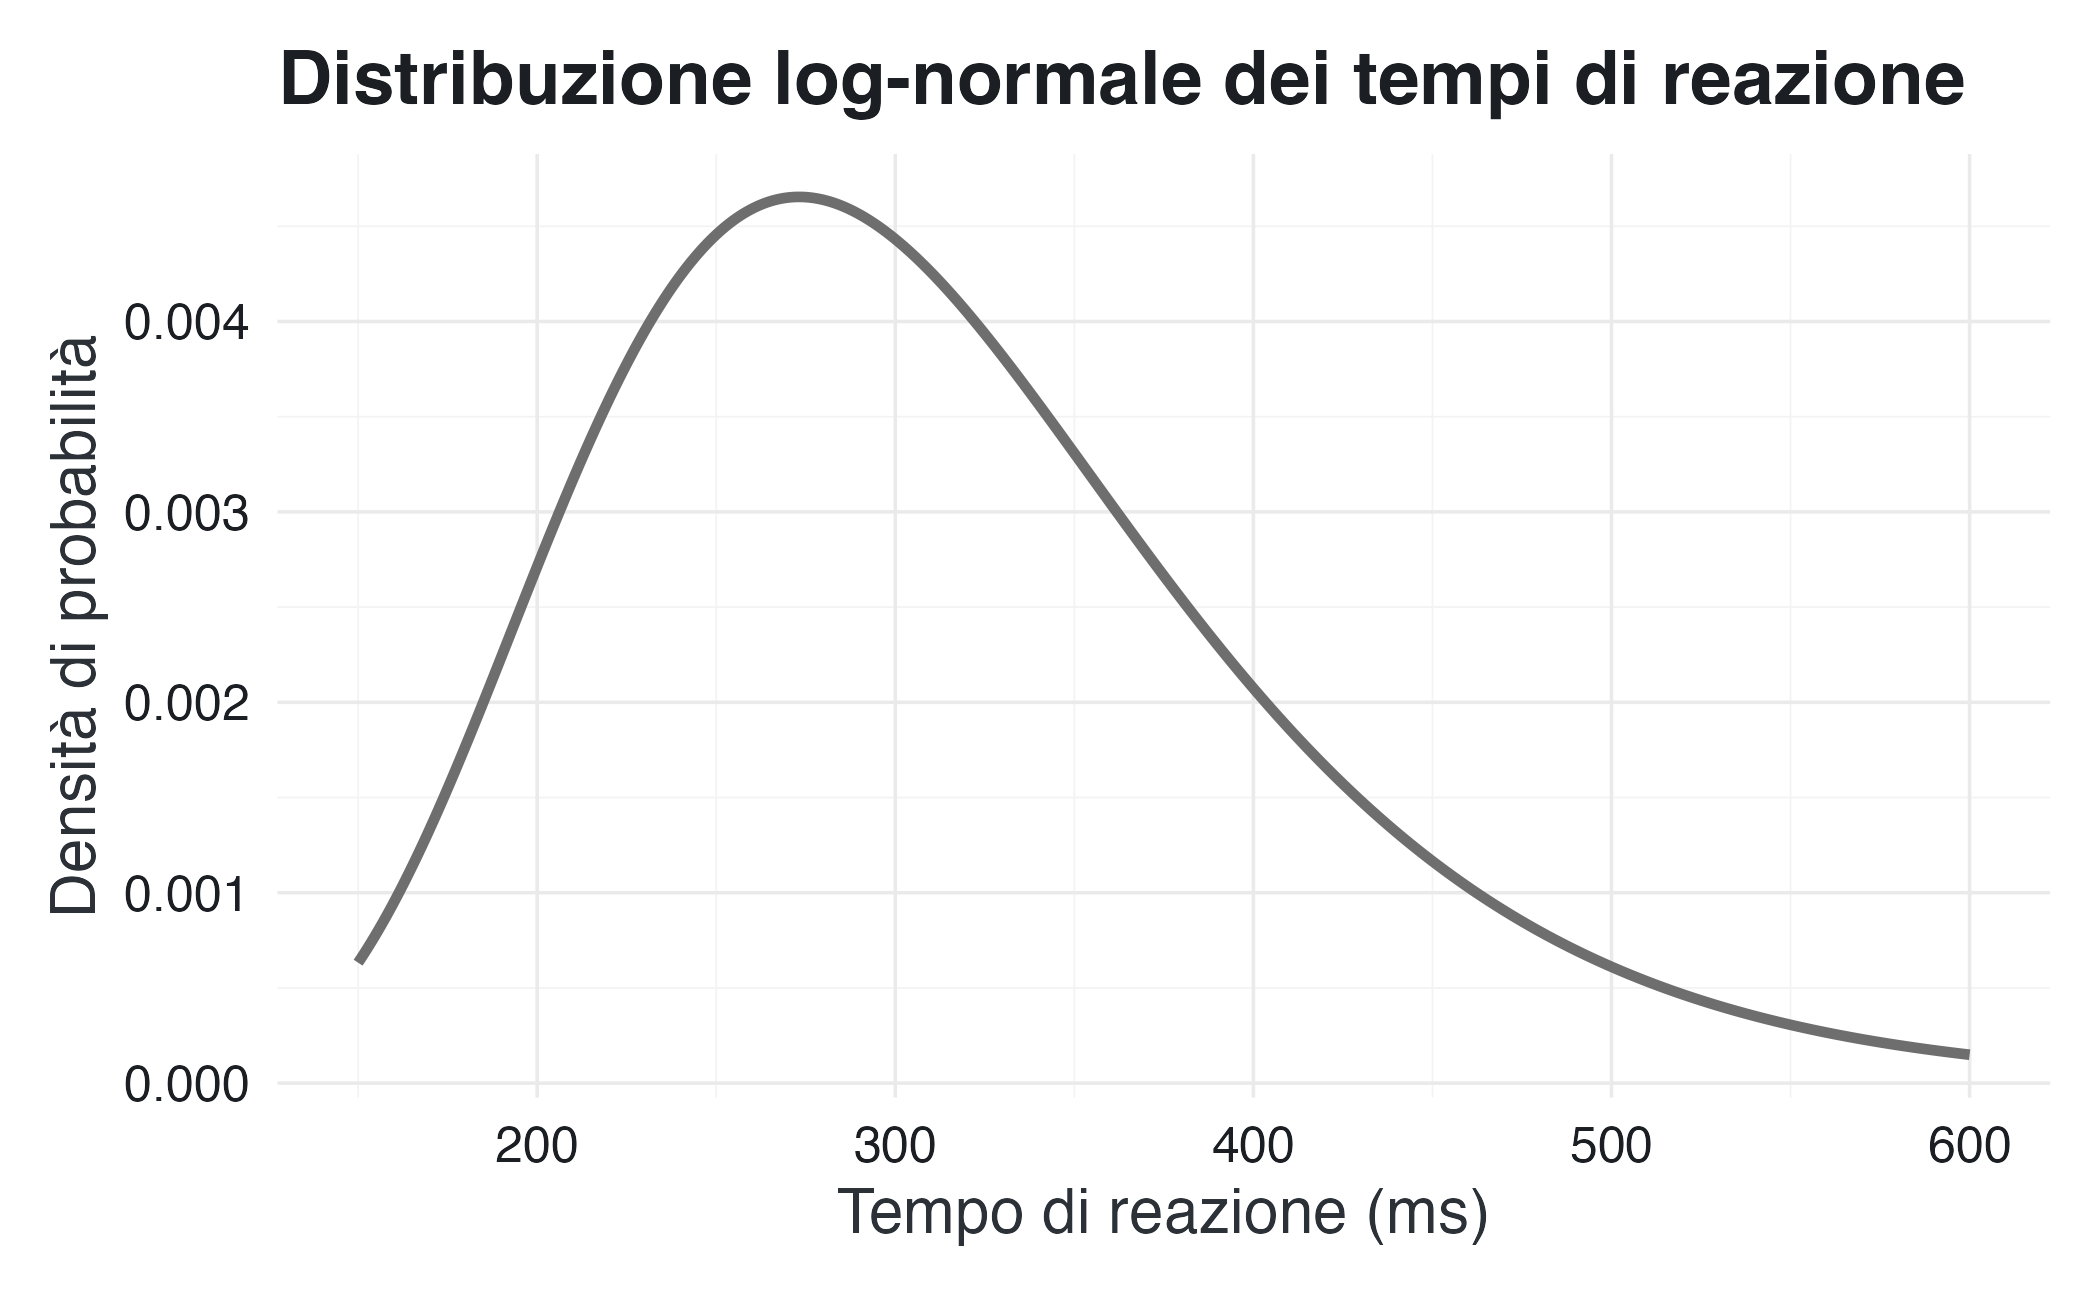
\includegraphics[width=0.85\linewidth,height=\textheight,keepaspectratio]{chapters/probability/06_random_var_files/figure-pdf/unnamed-chunk-2-1.png}

La probabilità che il tempo di reazione cada tra 300 e 400 ms è l'area
sotto la curva in quell'intervallo:

\begin{Shaded}
\begin{Highlighting}[]
\NormalTok{prob\_300\_400 }\OtherTok{\textless{}{-}} \FunctionTok{plnorm}\NormalTok{(}\DecValTok{400}\NormalTok{, }\AttributeTok{meanlog =}\NormalTok{ mu, }\AttributeTok{sdlog =}\NormalTok{ sigma) }\SpecialCharTok{{-}} 
                \FunctionTok{plnorm}\NormalTok{(}\DecValTok{300}\NormalTok{, }\AttributeTok{meanlog =}\NormalTok{ mu, }\AttributeTok{sdlog =}\NormalTok{ sigma)}
\FunctionTok{cat}\NormalTok{(}\StringTok{"P(300 ≤ T ≤ 400):"}\NormalTok{, }\FunctionTok{round}\NormalTok{(prob\_300\_400, }\DecValTok{3}\NormalTok{), }\StringTok{"}\SpecialCharTok{\textbackslash{}n}\StringTok{"}\NormalTok{)}
\CommentTok{\#\textgreater{} P(300 ≤ T ≤ 400): 0.329}
\end{Highlighting}
\end{Shaded}

\end{tcolorbox}

\section{Funzione di distribuzione cumulativa}\label{sec-cdf}

Esiste una descrizione che vale \emph{sia per le variabili discrete che
per quelle continue}: la \emph{funzione di distribuzione cumulativa}.

\begin{definition}[Funzione di distribuzione cumulativa
(CDF)]\protect\hypertarget{def-cdf}{}\label{def-cdf}

La \emph{funzione di distribuzione cumulativa} di una variabile casuale
\(X\) è la funzione

\[
F_X : \mathbb{R} \to [0,1]
\] definita da \(F_X(x) = P(X \leq x)\).

\end{definition}

Dal punto di vista epistemico, \(F_X(x)\) rappresenta il grado di
credenza che il valore di \(X\) non superi la soglia \(x\).

\subsection{Relazione con PMF e PDF}\label{relazione-con-pmf-e-pdf}

\begin{itemize}
\tightlist
\item
  \textbf{Per variabili continue}:
  \(F_X(x) = \int_{-\infty}^{x} f_X(t)\,dt\), e
  \(f_X(x) = \frac{d}{dx} F_X(x)\).
\item
  \textbf{Per variabili discrete}:
  \(F_X(x) = \sum_{x_i \leq x} p_X(x_i)\).
\end{itemize}

\begin{theorem}[Proprietà della
CDF]\protect\hypertarget{thm-cdf-properties}{}\label{thm-cdf-properties}

~

\begin{enumerate}
\def\labelenumi{\arabic{enumi}.}
\tightlist
\item
  \textbf{Monotonia non decrescente}: \(F_X(a) \leq F_X(b)\) per
  \(a < b\).
\item
  \textbf{Comportamento asintotico}:
  \(\lim_{x \to -\infty} F_X(x) = 0\),
  \(\lim_{x \to +\infty} F_X(x) = 1\).
\item
  \textbf{Continuità da destra}:
  \(\lim_{h \to 0^+} F_X(x + h) = F_X(x)\).
\end{enumerate}

\end{theorem}

\subsection{Ponte applicativo: uso della CDF per i cut-off
clinici}\label{ponte-applicativo-uso-della-cdf-per-i-cut-off-clinici}

La CDF è lo strumento naturale per calcolare la proporzione di individui
che cadono sotto una certa soglia. Se il punteggio \(X\) al PHQ-9 nella
popolazione clinica segue una certa distribuzione:

\begin{itemize}
\tightlist
\item
  \(F_X(9)\) = probabilità di punteggio ≤ 9 (depressione minima);
\item
  \(1 - F_X(19)\) = probabilità di depressione grave;
\item
  \(F_X(14) - F_X(9)\) = probabilità di depressione moderata.
\end{itemize}

\subsection{Connessione con il percorso
bayesiano}\label{connessione-con-il-percorso-bayesiano-1}

La CDF è lo strumento fondamentale per calcolare gli \emph{intervalli di
credibilità}. Se il parametro \(\theta\) ha distribuzione a posteriori
\(p(\theta \mid \text{dati})\):

\begin{itemize}
\tightlist
\item
  il \textbf{quantile} \(q_\alpha\) tale che
  \(F_\theta(q_\alpha) = \alpha\);
\item
  l'\textbf{intervallo di credibilità al 95\%} è
  \([q_{0.025}, q_{0.975}]\);
\item
  la \textbf{probabilità a posteriori} che \(\theta\) superi una soglia
  \(\theta_0\) è \(1 - F_\theta(\theta_0)\).
\end{itemize}

\section{Variabili casuali
multiple}\label{sec-multiple-random-variables}

In molti contesti è necessario modellare \emph{più fenomeni aleatori
simultaneamente}. Nello studio della comorbilità, ad esempio, è
necessario rappresentare congiuntamente ansia e depressione.

\subsection{Distribuzione congiunta}\label{distribuzione-congiunta}

\begin{definition}[Distribuzione
congiunta]\protect\hypertarget{def-joint-distribution}{}\label{def-joint-distribution}

Siano \(X\) e \(Y\) due variabili casuali discrete. La \emph{funzione di
massa di probabilità congiunta} è:

\[
p_{X,Y}(x,y) = P(X = x, Y = y).
\]

Essa assegna una probabilità a ciascuna coppia di valori \((x,y)\).

\end{definition}

\subsection{Esempio: ansia e
depressione}\label{esempio-ansia-e-depressione}

{\def\LTcaptype{none} % do not increment counter
\begin{longtable}[]{@{}llll@{}}
\toprule\noalign{}
& Depr. bassa & Depr. media & Depr. alta \\
\midrule\noalign{}
\endhead
\bottomrule\noalign{}
\endlastfoot
\textbf{Ansia bassa} & 0.25 & 0.10 & 0.05 \\
\textbf{Ansia media} & 0.08 & 0.15 & 0.07 \\
\textbf{Ansia alta} & 0.02 & 0.08 & 0.20 \\
\end{longtable}
}

La somma di tutte le celle è 1.
\(p_{X,Y}(\text{alta}, \text{alta}) = 0.20\).

\subsection{Distribuzioni marginali}\label{distribuzioni-marginali}

Le \emph{distribuzioni marginali} si ottengono sommando sulla variabile
da eliminare:

\[
p_X(x) = \sum_y p_{X,Y}(x,y), \qquad p_Y(y) = \sum_x p_{X,Y}(x,y).
\]

Nell'esempio: \(p_X(\text{ansia alta}) = 0.02 + 0.08 + 0.20 = 0.30\).

\subsection{Indipendenza stocastica}\label{indipendenza-stocastica}

Le variabili \(X\) e \(Y\) sono \emph{indipendenti} se:

\[
p_{X,Y}(x,y) = p_X(x) \cdot p_Y(y) \quad \text{per ogni } (x,y).
\]

Nell'esempio, ansia e depressione \emph{non} sono indipendenti:
\(0.20 \neq 0.30 \times 0.32 = 0.096\). Le due condizioni tendono a
co-occorrere più di quanto ci si aspetterebbe per caso.

\subsection{Ponte applicativo}\label{ponte-applicativo}

Nella pratica clinica, le relazioni tra ansia e depressione, tra sintomi
e funzionamento, richiedono tutte di modellare distribuzioni congiunte.
Nell'inferenza bayesiana, quando abbiamo più parametri, la distribuzione
a posteriori è una distribuzione congiunta su tutti i parametri.

\section*{Riflessioni conclusive}\label{riflessioni-conclusive-5}

\markright{Riflessioni conclusive}

Il concetto di \emph{variabile casuale} rappresenta il ponte
fondamentale tra la teoria della probabilità e l'analisi quantitativa
dei fenomeni psicologici. Ogni risultato, che si tratti di un punteggio,
di un tempo o di un conteggio, può essere tradotto in un oggetto
matematico sul quale è possibile applicare gli strumenti del calcolo
delle probabilità.

Le due principali classi di variabili casuali, \emph{discrete} e
\emph{continue}, richiedono formalizzazioni tecniche differenti (somme
vs integrali), ma si basano sullo stesso principio: descrivere la
distribuzione della credenza nello spazio dei possibili valori.

Per chi si avvicina all'inferenza bayesiana, questi concetti
costituiscono il \emph{vocabolario necessario} per:

\begin{itemize}
\tightlist
\item
  specificare le distribuzioni a priori sui parametri;
\item
  comprendere la funzione di verosimiglianza;
\item
  interpretare le distribuzioni a posteriori e gli intervalli di
  credibilità;
\item
  formulare domande probabilistiche sui fenomeni psicologici.
\end{itemize}

Nei capitoli successivi studieremo le \emph{famiglie parametriche di
distribuzioni}, come la distribuzione Beta, la distribuzione Normale, la
distribuzione Binomiale, la distribuzione di Poisson e altre, che
costituiscono i mattoni elementari della modellazione bayesiana.

\section*{Punti chiave da ricordare}\label{punti-chiave-da-ricordare-5}
\addcontentsline{toc}{section}{Punti chiave da ricordare}

\markright{Punti chiave da ricordare}

\begin{tcolorbox}[enhanced jigsaw, arc=.35mm, bottomrule=.15mm, bottomtitle=1mm, breakable, colback=white, colbacktitle=quarto-callout-important-color!10!white, colframe=quarto-callout-important-color-frame, coltitle=black, left=2mm, leftrule=.75mm, opacityback=0, opacitybacktitle=0.6, rightrule=.15mm, title=\textcolor{quarto-callout-important-color}{\faExclamation}\hspace{0.5em}{Importante}, titlerule=0mm, toprule=.15mm, toptitle=1mm]

\begin{enumerate}
\def\labelenumi{\arabic{enumi}.}
\tightlist
\item
  \textbf{Variabile casuale come funzione}

  \begin{itemize}
  \tightlist
  \item
    \(X: \Omega \to \mathbb{R}\) associa a ogni esito un valore
    numerico.
  \item
    La funzione è deterministica; l'incertezza riguarda quale esito si
    realizzerà.
  \item
    Permette di passare da eventi qualitativi a quantità analizzabili.
  \end{itemize}
\item
  \textbf{Discrete vs Continue}

  \begin{itemize}
  \tightlist
  \item
    Discrete: valori numerabili (punteggi, conteggi).
  \item
    Continue: valori in intervalli (tempi, misure fisiologiche).
  \item
    Strumenti diversi: somme vs integrali.
  \end{itemize}
\item
  \textbf{PMF per variabili discrete}

  \begin{itemize}
  \tightlist
  \item
    \(p_X(x) = P(X = x)\) è una probabilità.
  \item
    \(\sum_x p_X(x) = 1\).
  \end{itemize}
\item
  \textbf{PDF per variabili continue}

  \begin{itemize}
  \tightlist
  \item
    \(f_X(x)\) è una densità, non una probabilità.
  \item
    \(P(a \leq X \leq b) = \int_a^b f_X(x) \, dx\).
  \item
    \(P(X = x) = 0\) per ogni \(x\).
  \end{itemize}
\item
  \textbf{CDF come rappresentazione unificata}

  \begin{itemize}
  \tightlist
  \item
    \(F_X(x) = P(X \leq x)\) funziona per entrambi i tipi.
  \item
    Fondamentale per quantili e intervalli di credibilità.
  \end{itemize}
\item
  \textbf{Variabili multiple}

  \begin{itemize}
  \tightlist
  \item
    La distribuzione congiunta descrive l'incertezza su combinazioni.
  \item
    Marginalizzazione: eliminare una variabile sommando/integrando.
  \item
    Indipendenza: \(p_{X,Y}(x,y) = p_X(x) \cdot p_Y(y)\).
  \end{itemize}
\end{enumerate}

\textbf{Formule essenziali:}

\[
\text{PMF: } p_X(x) = P(X = x), \quad \sum_x p_X(x) = 1
\]

\[
\text{PDF: } P(a \leq X \leq b) = \int_a^b f_X(x) \, dx, \quad \int_{-\infty}^{+\infty} f_X(x) \, dx = 1
\]

\[
\text{CDF: } F_X(x) = P(X \leq x)
\]

\[
\text{Marginale: } p_X(x) = \sum_y p_{X,Y}(x,y)
\]

\end{tcolorbox}

\begin{tcolorbox}[enhanced jigsaw, arc=.35mm, bottomrule=.15mm, bottomtitle=1mm, breakable, colback=white, colbacktitle=quarto-callout-note-color!10!white, colframe=quarto-callout-note-color-frame, coltitle=black, left=2mm, leftrule=.75mm, opacityback=0, opacitybacktitle=0.6, rightrule=.15mm, title=\textcolor{quarto-callout-note-color}{\faInfo}\hspace{0.5em}{Informazioni sull'ambiente di sviluppo}, titlerule=0mm, toprule=.15mm, toptitle=1mm]

\begin{Shaded}
\begin{Highlighting}[]
\FunctionTok{sessionInfo}\NormalTok{()}
\CommentTok{\#\textgreater{} R version 4.6.1 (2026{-}06{-}24)}
\CommentTok{\#\textgreater{} Platform: aarch64{-}apple{-}darwin23}
\CommentTok{\#\textgreater{} Running under: macOS Tahoe 26.5.2}
\CommentTok{\#\textgreater{} }
\CommentTok{\#\textgreater{} Matrix products: default}
\CommentTok{\#\textgreater{} BLAS:   /Library/Frameworks/R.framework/Versions/4.6/Resources/lib/libRblas.0.dylib }
\CommentTok{\#\textgreater{} LAPACK: /Library/Frameworks/R.framework/Versions/4.6/Resources/lib/libRlapack.dylib;  LAPACK version 3.12.1}
\CommentTok{\#\textgreater{} }
\CommentTok{\#\textgreater{} locale:}
\CommentTok{\#\textgreater{} [1] C.UTF{-}8/UTF{-}8/C.UTF{-}8/C/C.UTF{-}8/C.UTF{-}8}
\CommentTok{\#\textgreater{} }
\CommentTok{\#\textgreater{} time zone: Europe/Zagreb}
\CommentTok{\#\textgreater{} tzcode source: internal}
\CommentTok{\#\textgreater{} }
\CommentTok{\#\textgreater{} attached base packages:}
\CommentTok{\#\textgreater{} [1] stats     graphics  grDevices utils     datasets  methods   base     }
\CommentTok{\#\textgreater{} }
\CommentTok{\#\textgreater{} other attached packages:}
\CommentTok{\#\textgreater{}  [1] ragg\_1.5.2            tinytable\_0.17.0      withr\_3.0.3          }
\CommentTok{\#\textgreater{}  [4] systemfonts\_1.3.2     patchwork\_1.3.2       ggdist\_3.3.3         }
\CommentTok{\#\textgreater{}  [7] tidybayes\_3.0.7       bayesplot\_1.15.0      ggplot2\_4.0.3        }
\CommentTok{\#\textgreater{} [10] reliabilitydiag\_0.2.1 priorsense\_1.2.0      posterior\_1.7.0      }
\CommentTok{\#\textgreater{} [13] loo\_2.10.0            rstan\_2.32.7          StanHeaders\_2.32.10  }
\CommentTok{\#\textgreater{} [16] brms\_2.23.0           Rcpp\_1.1.2            sessioninfo\_1.2.4    }
\CommentTok{\#\textgreater{} [19] conflicted\_1.2.0      janitor\_2.2.1         matrixStats\_1.5.0    }
\CommentTok{\#\textgreater{} [22] modelr\_0.1.11         tibble\_3.3.1          dplyr\_1.2.1          }
\CommentTok{\#\textgreater{} [25] tidyr\_1.3.2           rio\_1.3.0             here\_1.0.2           }
\CommentTok{\#\textgreater{} }
\CommentTok{\#\textgreater{} loaded via a namespace (and not attached):}
\CommentTok{\#\textgreater{}  [1] svUnit\_1.0.8          tidyselect\_1.2.1      farver\_2.1.2         }
\CommentTok{\#\textgreater{}  [4] S7\_0.2.2              fastmap\_1.2.0         tensorA\_0.36.2.1     }
\CommentTok{\#\textgreater{}  [7] digest\_0.6.39         timechange\_0.4.0      estimability\_2.0.0   }
\CommentTok{\#\textgreater{} [10] lifecycle\_1.0.5       magrittr\_2.0.5        compiler\_4.6.1       }
\CommentTok{\#\textgreater{} [13] rlang\_1.3.0           tools\_4.6.1           yaml\_2.3.12          }
\CommentTok{\#\textgreater{} [16] knitr\_1.51            labeling\_0.4.3        bridgesampling\_1.2{-}1 }
\CommentTok{\#\textgreater{} [19] pkgbuild\_1.4.8        curl\_7.1.0            RColorBrewer\_1.1{-}3   }
\CommentTok{\#\textgreater{} [22] abind\_1.4{-}8           purrr\_1.2.2           grid\_4.6.1           }
\CommentTok{\#\textgreater{} [25] stats4\_4.6.1          xtable\_1.8{-}8          inline\_0.3.21        }
\CommentTok{\#\textgreater{} [28] emmeans\_2.0.4         scales\_1.4.0          cli\_3.6.6            }
\CommentTok{\#\textgreater{} [31] mvtnorm\_1.4{-}2         rmarkdown\_2.31        generics\_0.1.4       }
\CommentTok{\#\textgreater{} [34] otel\_0.2.0            RcppParallel\_5.1.11{-}2 cachem\_1.1.0         }
\CommentTok{\#\textgreater{} [37] stringr\_1.6.0         parallel\_4.6.1        vctrs\_0.7.3          }
\CommentTok{\#\textgreater{} [40] V8\_8.2.0              Matrix\_1.7{-}5          jsonlite\_2.0.0       }
\CommentTok{\#\textgreater{} [43] arrayhelpers\_1.1{-}1    glue\_1.8.1            codetools\_0.2{-}20     }
\CommentTok{\#\textgreater{} [46] distributional\_0.8.1  lubridate\_1.9.5       stringi\_1.8.7        }
\CommentTok{\#\textgreater{} [49] gtable\_0.3.6          QuickJSR\_1.10.0       pillar\_1.11.1        }
\CommentTok{\#\textgreater{} [52] htmltools\_0.5.9       Brobdingnag\_1.2{-}9     R6\_2.6.1             }
\CommentTok{\#\textgreater{} [55] textshaping\_1.0.5     rprojroot\_2.1.1       evaluate\_1.0.5       }
\CommentTok{\#\textgreater{} [58] lattice\_0.22{-}9        backports\_1.5.1       memoise\_2.0.1        }
\CommentTok{\#\textgreater{} [61] broom\_1.0.13          snakecase\_0.11.1      rstantools\_2.6.0     }
\CommentTok{\#\textgreater{} [64] coda\_0.19{-}4.1         gridExtra\_2.3.1       nlme\_3.1{-}170         }
\CommentTok{\#\textgreater{} [67] checkmate\_2.3.4       xfun\_0.60             pkgconfig\_2.0.3}
\end{Highlighting}
\end{Shaded}

\end{tcolorbox}

\chapter{Distribuzioni di massa e di densità}\label{sec-prob-distr}

\section*{Introduzione}\label{introduzione-6}

\markright{Introduzione}

Nel capitolo precedente (Capitolo~\ref{sec-prob-random-var}) abbiamo
introdotto le \textbf{variabili casuali} come funzioni che associano
valori numerici agli esiti di un esperimento aleatorio. Abbiamo distinto
tra variabili casuali \textbf{discrete}, che assumono un insieme finito
o numerabile di valori, e variabili casuali \textbf{continue}, che
possono assumere qualsiasi valore all'interno di un intervallo. Per
ciascun caso, abbiamo definito formalmente la \emph{funzione di massa di
probabilità} (PMF) e la \emph{funzione di densità di probabilità} (PDF)
come strumenti fondamentali per descrivere l'incertezza sui valori
assunti dalla variabile.

Questo capitolo ha lo scopo di approfondire la \textbf{comprensione
intuitiva, geometrica e operativa} di tali concetti. Vedremo come la PMF
assegni ``pesi'' discreti a singoli valori, mentre la PDF distribuisca
la probabilità in modo continuo lungo la retta reale, rendendo
necessario l'uso dell'integrazione per calcolare la probabilità
associata a intervalli di valori. In questo contesto affronteremo anche
il noto ``paradosso'' secondo cui, per una variabile casuale continua,
la probabilità di osservare un valore esatto è sempre pari a zero,
mostrando come questa proprietà non sia affatto paradossale, ma una
conseguenza naturale della struttura matematica del continuo.

Un aspetto centrale della trattazione riguarda inoltre la
\textbf{distinzione interpretativa} tra l'approccio frequentista e
quello bayesiano alle distribuzioni di probabilità. Nel paradigma
frequentista, la funzione di densità descrive il comportamento dei dati
in ipotetiche ripetizioni dell'esperimento. Nell'approccio bayesiano,
invece, la PDF rappresenta il \textbf{grado di credenza} assegnato ai
possibili valori di una quantità incerta, come un parametro o una
grandezza latente. Questa differenza concettuale, apparentemente
sottile, ha implicazioni profonde per il modo in cui interpretiamo le
distribuzioni, calcoliamo le probabilità e traiamo conclusioni
inferenziali.

\begin{tcolorbox}[enhanced jigsaw, arc=.35mm, bottomrule=.15mm, bottomtitle=1mm, breakable, colback=white, colbacktitle=quarto-callout-tip-color!10!white, colframe=quarto-callout-tip-color-frame, coltitle=black, left=2mm, leftrule=.75mm, opacityback=0, opacitybacktitle=0.6, rightrule=.15mm, title=\textcolor{quarto-callout-tip-color}{\faLightbulb}\hspace{0.5em}{Prerequisiti}, titlerule=0mm, toprule=.15mm, toptitle=1mm]

Per seguire questo capitolo è necessario aver letto:

\begin{itemize}
\tightlist
\item
  Capitolo~\ref{sec-prob-random-var} --- \textbf{fondamentale}
\end{itemize}

Questo capitolo approfondisce i concetti di PMF e PDF introdotti nel
Capitolo 6, fornendo una comprensione intuitiva, geometrica e operativa.

Conoscenze matematiche richieste:

\begin{itemize}
\tightlist
\item
  Appendice~\ref{sec-apx-calculus} - per comprendere l'integrale come
  area sotto una curva
\item
  Familiarità con il concetto di limite per capire il passaggio da
  istogrammi a densità continue
\end{itemize}

Letture complementari consigliate:

\begin{itemize}
\tightlist
\item
  Blitzstein, J. K., \& Hwang, J. (2019). \emph{Introduction to
  Probability} (2nd ed.), capitolo ``Random variables and their
  distributions'' (\citeproc{ref-blitzstein2019introduction}{Blitzstein
  \& Hwang, 2019})
\end{itemize}

\end{tcolorbox}

\subsection*{Panoramica del capitolo}\label{panoramica-del-capitolo-2}

\begin{itemize}
\tightlist
\item
  Distinzione operativa tra massa di probabilità e densità di
  probabilità.
\item
  Dagli istogrammi alle funzioni di densità: il limite continuo.
\item
  Il ``paradosso'' della probabilità zero per valori esatti.
\item
  La funzione di distribuzione cumulativa come rappresentazione
  unificata.
\item
  Interpretazioni bayesiana e frequentista delle distribuzioni.
\end{itemize}

\begin{tcolorbox}[enhanced jigsaw, arc=.35mm, bottomrule=.15mm, bottomtitle=1mm, breakable, colback=white, colbacktitle=quarto-callout-caution-color!10!white, colframe=quarto-callout-caution-color-frame, coltitle=black, left=2mm, leftrule=.75mm, opacityback=0, opacitybacktitle=0.6, rightrule=.15mm, title=\textcolor{quarto-callout-caution-color}{\faFire}\hspace{0.5em}{Preparazione del Notebook}, titlerule=0mm, toprule=.15mm, toptitle=1mm]

\begin{Shaded}
\begin{Highlighting}[]
\NormalTok{here}\SpecialCharTok{::}\FunctionTok{here}\NormalTok{(}\StringTok{"code"}\NormalTok{, }\StringTok{"\_common.R"}\NormalTok{) }\SpecialCharTok{|\textgreater{}} 
  \FunctionTok{source}\NormalTok{()}
\CommentTok{\# Riapplica il tema per sicurezza}
\FunctionTok{apply\_visual\_theme}\NormalTok{()}
\end{Highlighting}
\end{Shaded}

\end{tcolorbox}

\section{Dalla massa alla densità di
probabilità}\label{dalla-massa-alla-densituxe0-di-probabilituxe0}

La distinzione tra variabili casuali \textbf{discrete} e
\textbf{continue} non è solo tecnica: riflette due modi profondamente
diversi in cui la probabilità si distribuisce sui valori possibili. Nel
caso discreto, si può assegnare una probabilità positiva a ogni singolo
valore; nel caso continuo, invece, la probabilità non si concentra su
punti isolati ma si \textbf{distribuisce su un continuum}, per cui sono
assegnabili solo le probabilità associate a intervalli.

Questa differenza concettuale è cruciale per comprendere correttamente
il ruolo delle funzioni di massa e di densità di probabilità.

\section{La funzione di massa di
probabilità}\label{la-funzione-di-massa-di-probabilituxe0}

Per una variabile casuale discreta \(X\) che assume valori nell'insieme
\[
\mathcal{X} = {x_1, x_2, \ldots},
\] la \textbf{funzione di massa di probabilità} (PMF) associa a ciascun
valore possibile la probabilità corrispondente: \[
p_X(x) = P(X = x).
\]

Il termine \emph{massa} evoca una metafora fisica appropriata: la
probabilità può essere immaginata come una collezione di \textbf{pesi
discreti} collocati sui valori possibili della variabile. Ogni valore
\(x_i\) è associato a una quantità \(p_X(x_i)\) e la somma totale delle
masse deve essere pari a 1. In questo contesto, è perfettamente lecito
``concentrare'' una parte rilevante della probabilità in pochi punti
specifici.

\begin{tcolorbox}[enhanced jigsaw, arc=.35mm, bottomrule=.15mm, bottomtitle=1mm, breakable, colback=white, colbacktitle=quarto-callout-note-color!10!white, colframe=quarto-callout-note-color-frame, coltitle=black, left=2mm, leftrule=.75mm, opacityback=0, opacitybacktitle=0.6, rightrule=.15mm, title=\textcolor{quarto-callout-note-color}{\faInfo}\hspace{0.5em}{Esempio: soddisfazione lavorativa su scala Likert}, titlerule=0mm, toprule=.15mm, toptitle=1mm]

\subsubsection*{Distribuzione tipica delle
risposte}\label{distribuzione-tipica-delle-risposte}

Consideriamo le risposte a un item sulla soddisfazione lavorativa,
misurata su una scala Likert a 5 punti (1 = ``molto insoddisfatto'', 5 =
``molto soddisfatto''). In molte popolazioni lavorative, le risposte
tendono a concentrarsi sui valori centrali e moderatamente positivi, con
una distribuzione asimmetrica:

{\def\LTcaptype{none} % do not increment counter
\begin{longtable}[]{@{}cccccc@{}}
\toprule\noalign{}
Risposta & 1 (molto insod.) & 2 & 3 & 4 & 5 (molto sodd.) \\
\midrule\noalign{}
\endhead
\bottomrule\noalign{}
\endlastfoot
\(p_X(x)\) & 0.05 & 0.10 & 0.25 & 0.40 & 0.20 \\
\end{longtable}
}

Questa PMF riflette un pattern tipico: pochi lavoratori dichiarano una
forte insoddisfazione, la maggior parte si colloca su livelli moderati o
buoni, e una minoranza esprime una piena soddisfazione. La coerenza
della distribuzione è immediatamente verificabile:

\[
\sum_{x=1}^{5} p_X(x) = 0.05 + 0.10 + 0.25 + 0.40 + 0.20 = 1.
\]

Simulando 10,000 risposte secondo questa distribuzione e confrontando le
frequenze empiriche con la PMF teorica, osserviamo una chiara
convergenza:

\begin{Shaded}
\begin{Highlighting}[]
\FunctionTok{set.seed}\NormalTok{(}\DecValTok{123}\NormalTok{)}
\NormalTok{prob\_teoriche }\OtherTok{\textless{}{-}} \FunctionTok{c}\NormalTok{(}\FloatTok{0.05}\NormalTok{, }\FloatTok{0.10}\NormalTok{, }\FloatTok{0.25}\NormalTok{, }\FloatTok{0.40}\NormalTok{, }\FloatTok{0.20}\NormalTok{)}
\NormalTok{n\_risposte }\OtherTok{\textless{}{-}} \DecValTok{10000}

\NormalTok{risposte }\OtherTok{\textless{}{-}} \FunctionTok{sample}\NormalTok{(}\DecValTok{1}\SpecialCharTok{:}\DecValTok{5}\NormalTok{, }\AttributeTok{size =}\NormalTok{ n\_risposte, }\AttributeTok{replace =} \ConstantTok{TRUE}\NormalTok{, }\AttributeTok{prob =}\NormalTok{ prob\_teoriche)}
\NormalTok{freq\_rel }\OtherTok{\textless{}{-}} \FunctionTok{table}\NormalTok{(risposte) }\SpecialCharTok{/}\NormalTok{ n\_risposte}

\NormalTok{df }\OtherTok{\textless{}{-}} \FunctionTok{data.frame}\NormalTok{(}
  \AttributeTok{valore =} \DecValTok{1}\SpecialCharTok{:}\DecValTok{5}\NormalTok{,}
  \AttributeTok{empirica =} \FunctionTok{as.numeric}\NormalTok{(freq\_rel),}
  \AttributeTok{teorica =}\NormalTok{ prob\_teoriche}
\NormalTok{)}

\FunctionTok{ggplot}\NormalTok{(df, }\FunctionTok{aes}\NormalTok{(}\AttributeTok{x =} \FunctionTok{factor}\NormalTok{(valore))) }\SpecialCharTok{+}
  \FunctionTok{geom\_col}\NormalTok{(}\FunctionTok{aes}\NormalTok{(}\AttributeTok{y =}\NormalTok{ empirica), }\AttributeTok{alpha =} \FloatTok{0.7}\NormalTok{, }\AttributeTok{width =} \FloatTok{0.6}\NormalTok{) }\SpecialCharTok{+}
  \FunctionTok{geom\_point}\NormalTok{(}\FunctionTok{aes}\NormalTok{(}\AttributeTok{y =}\NormalTok{ teorica), }\AttributeTok{size =} \DecValTok{4}\NormalTok{) }\SpecialCharTok{+}
  \FunctionTok{scale\_fill\_binary}\NormalTok{() }\SpecialCharTok{+}
  \FunctionTok{labs}\NormalTok{(}
    \AttributeTok{x =} \StringTok{"Livello di soddisfazione"}\NormalTok{, }
    \AttributeTok{y =} \StringTok{"Probabilità / Frequenza relativa"}\NormalTok{,}
    \AttributeTok{title =} \StringTok{"PMF della soddisfazione lavorativa (scala Likert 1{-}5)"}
\NormalTok{  ) }
\end{Highlighting}
\end{Shaded}

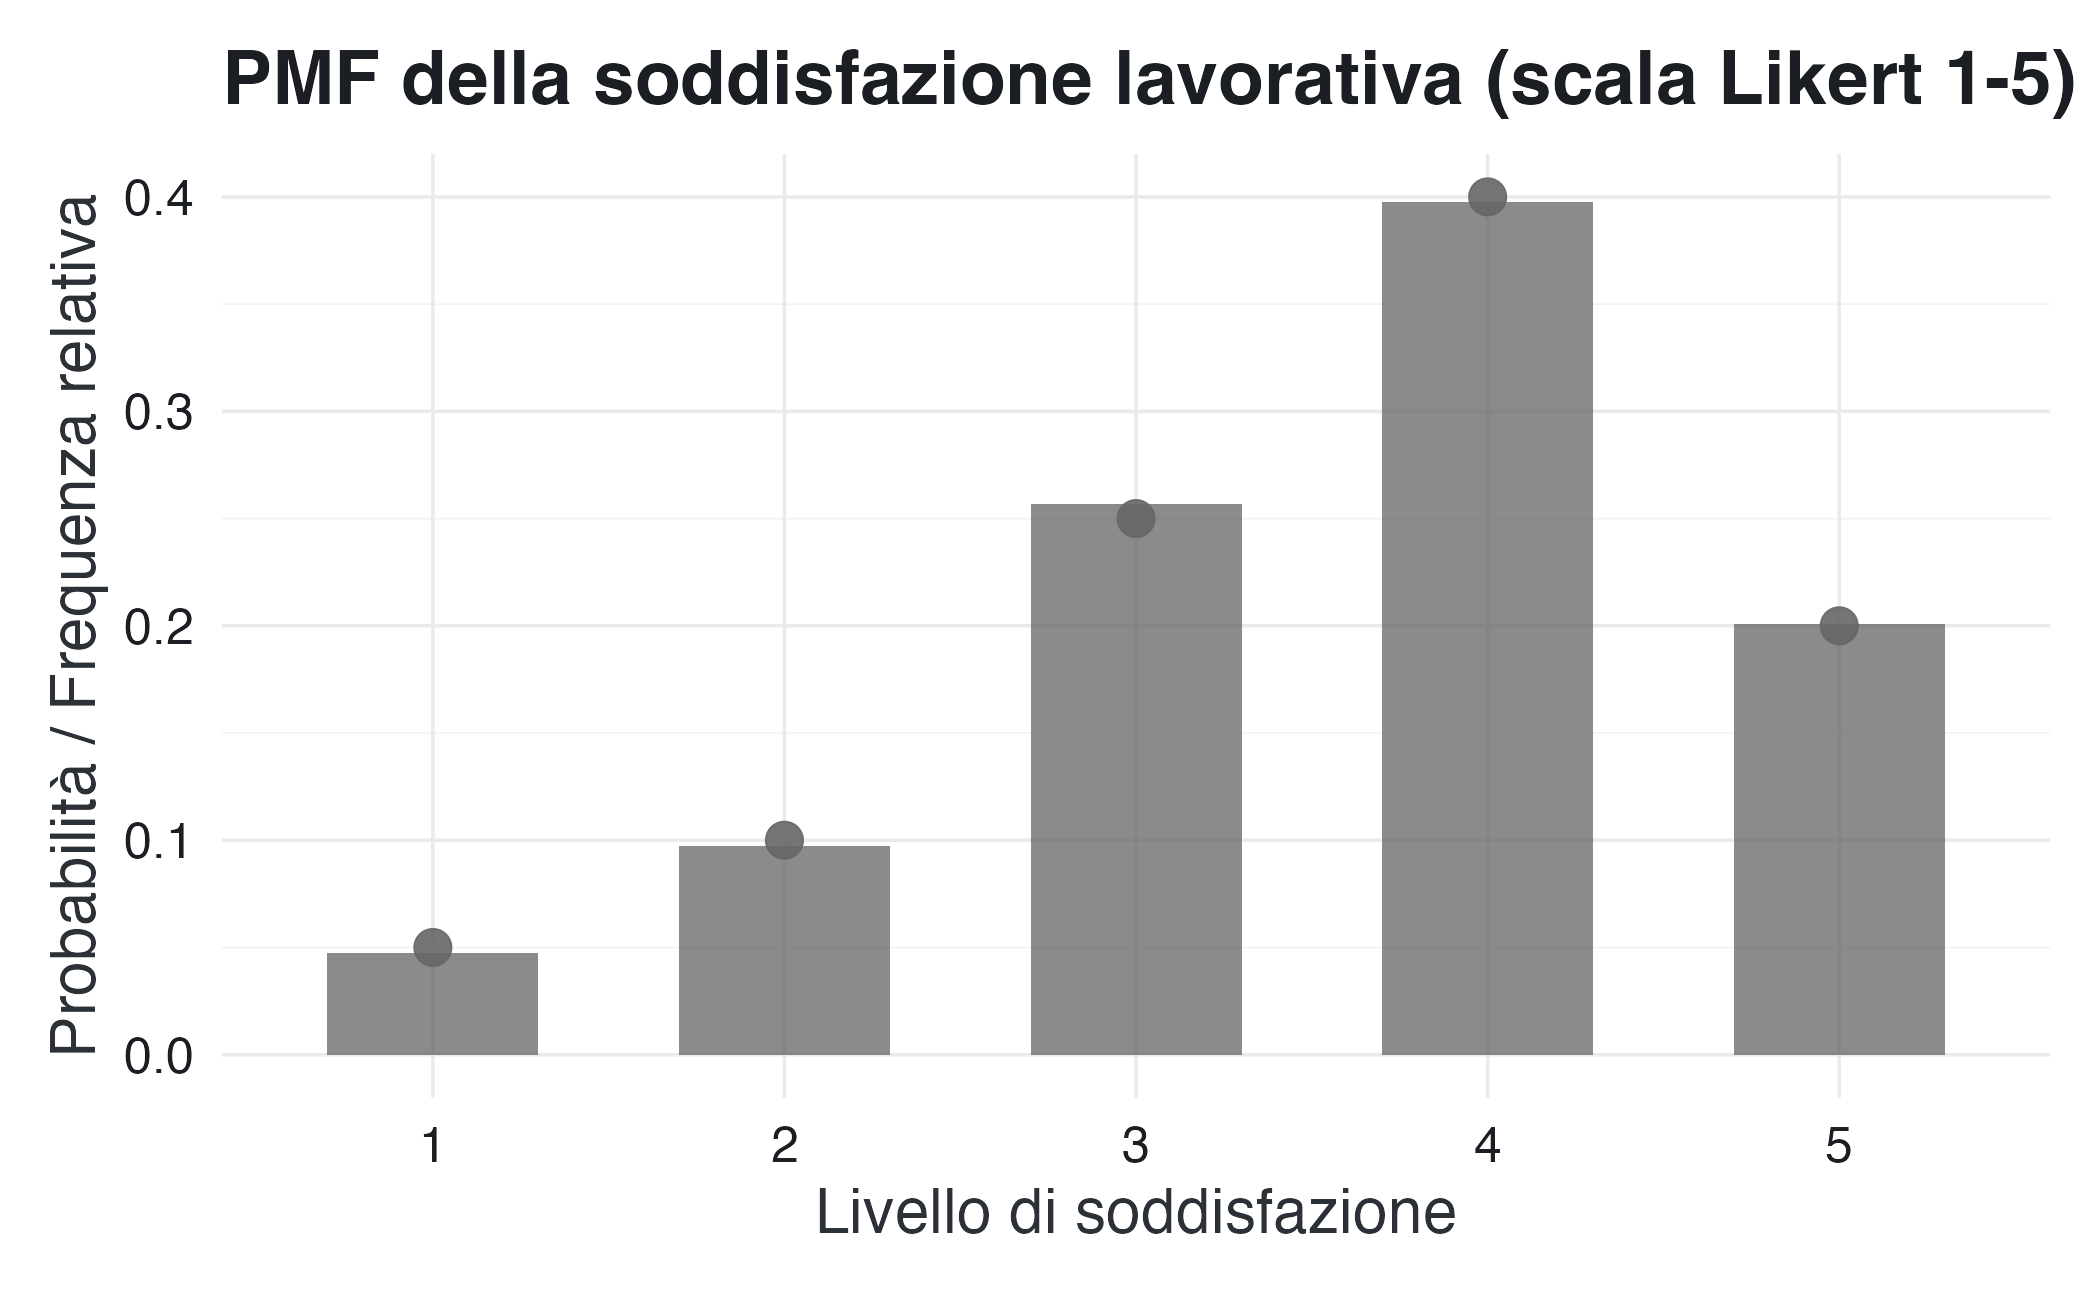
\includegraphics[width=0.85\linewidth,height=\textheight,keepaspectratio]{chapters/probability/07_prob_distributions_files/figure-pdf/unnamed-chunk-2-1.png}

Da questa distribuzione possiamo calcolare probabilità di interesse
pratico. Ad esempio, la probabilità che un lavoratore riporti almeno un
livello di soddisfazione ``buono'' (4 o 5) è:

\[
P(X \geq 4) = p_X(4) + p_X(5) = 0.40 + 0.20 = 0.60.
\]

La probabilità di insoddisfazione (1 o 2) è invece: \[
P(X \leq 2) = p_X(1) + p_X(2) = 0.05 + 0.10 = 0.15.
\]

Questa convergenza tra frequenze empiriche e probabilità teoriche non
\textbf{definisce} le probabilità, ma ne verifica la coerenza: un
sistema di credenze coerente produce il comportamento empirico atteso
quando viene sottoposto a prove ripetute.

\end{tcolorbox}

\section{La funzione di densità di
probabilità}\label{la-funzione-di-densituxe0-di-probabilituxe0}

Nel caso delle variabili casuali continue, questo approccio non è più
possibile. Non è possibile assegnare probabilità positive ai singoli
valori, in quanto i punti sono infiniti e la somma delle probabilità
divergerebbe. La soluzione concettuale consiste nel passare dalla
``massa'' alla ``densità''.

Invece di chiederci quanta probabilità c'è \emph{in} un punto, ci
chiediamo quanta probabilità c'è \emph{attorno} a un punto per unità di
lunghezza.

\begin{definition}[Funzione di densità di
probabilità]\protect\hypertarget{def-pdf}{}\label{def-pdf}

Una funzione

\[
f_X : \mathbb{R} \to [0, +\infty)
\]\\
è una \emph{funzione di densità di probabilità} (PDF) per una variabile
casuale continua \(X\) se, per ogni intervallo
\([a,b] \subseteq \mathbb{R}\),

\[
P(a \leq X \leq b) = \int_a^b f_X(x)\,dx,
\] e se soddisfa la condizione di normalizzazione

\[
\int_{-\infty}^{+\infty} f_X(x)\,dx = 1.
\]

La densità \(f_X(x)\) misura la \textbf{concentrazione locale della
probabilità} in prossimità del punto \(x\). Un valore elevato di
\(f_X(x)\) indica che, in un intorno molto piccolo di \(x\), si
concentra una probabilità relativamente maggiore rispetto alle regioni
con densità inferiore.

È importante notare che la densità non rappresenta una probabilità
puntuale: per una variabile continua la probabilità che \(X\) assuma
esattamente un singolo valore è sempre zero, \(P(X = x) = 0\). La
probabilità è un'area sotto la curva della PDF, non un'altezza.

\section{Dagli istogrammi alle
densità}\label{dagli-istogrammi-alle-densituxe0}

Un modo particolarmente intuitivo per comprendere la PDF consiste nel
considerarla come il \textbf{limite ideale di un istogramma}:
all'aumentare delle osservazioni e al ridursi della larghezza delle
classi, il profilo dell'istogramma delle frequenze relative tende a una
curva liscia che approssima la funzione di densità teorica.

Per illustrare questo concetto, consideriamo la distribuzione del
quoziente intellettivo (QI) nella popolazione generale. Il QI è
convenzionalmente definito con una media \(\mu = 100\) e una deviazione
standard \(\sigma = 15\), e segue approssimativamente una distribuzione
normale. Osserviamo come l'istogramma tenda alla PDF teorica
all'aumentare della dimensione campionaria:

\begin{Shaded}
\begin{Highlighting}[]
\FunctionTok{set.seed}\NormalTok{(}\DecValTok{42}\NormalTok{)}
\NormalTok{mu }\OtherTok{\textless{}{-}} \DecValTok{100}
\NormalTok{sigma }\OtherTok{\textless{}{-}} \DecValTok{15}

\NormalTok{n\_piccolo }\OtherTok{\textless{}{-}} \DecValTok{50}
\NormalTok{n\_grande }\OtherTok{\textless{}{-}} \DecValTok{20000}

\NormalTok{x\_piccolo }\OtherTok{\textless{}{-}} \FunctionTok{rnorm}\NormalTok{(n\_piccolo, }\AttributeTok{mean =}\NormalTok{ mu, }\AttributeTok{sd =}\NormalTok{ sigma)}
\NormalTok{x\_grande }\OtherTok{\textless{}{-}} \FunctionTok{rnorm}\NormalTok{(n\_grande, }\AttributeTok{mean =}\NormalTok{ mu, }\AttributeTok{sd =}\NormalTok{ sigma)}

\NormalTok{x\_seq }\OtherTok{\textless{}{-}} \FunctionTok{seq}\NormalTok{(}\DecValTok{40}\NormalTok{, }\DecValTok{160}\NormalTok{, }\AttributeTok{length.out =} \DecValTok{200}\NormalTok{)}
\NormalTok{y\_teorica }\OtherTok{\textless{}{-}} \FunctionTok{dnorm}\NormalTok{(x\_seq, }\AttributeTok{mean =}\NormalTok{ mu, }\AttributeTok{sd =}\NormalTok{ sigma)}
\NormalTok{df\_teorica }\OtherTok{\textless{}{-}} \FunctionTok{data.frame}\NormalTok{(}\AttributeTok{x =}\NormalTok{ x\_seq, }\AttributeTok{y =}\NormalTok{ y\_teorica)}

\NormalTok{p1 }\OtherTok{\textless{}{-}} \FunctionTok{ggplot}\NormalTok{(}\FunctionTok{data.frame}\NormalTok{(}\AttributeTok{x =}\NormalTok{ x\_piccolo), }\FunctionTok{aes}\NormalTok{(}\AttributeTok{x =}\NormalTok{ x)) }\SpecialCharTok{+}
  \FunctionTok{geom\_histogram}\NormalTok{(}\FunctionTok{aes}\NormalTok{(}\AttributeTok{y =} \FunctionTok{after\_stat}\NormalTok{(density)), }\AttributeTok{bins =} \DecValTok{15}\NormalTok{,}
                 \AttributeTok{color =} \StringTok{"white"}\NormalTok{, }\AttributeTok{alpha =} \FloatTok{0.7}\NormalTok{) }\SpecialCharTok{+}
  \FunctionTok{geom\_line}\NormalTok{(}\AttributeTok{data =}\NormalTok{ df\_teorica, }\FunctionTok{aes}\NormalTok{(}\AttributeTok{x =}\NormalTok{ x, }\AttributeTok{y =}\NormalTok{ y),}
            \AttributeTok{linewidth =} \DecValTok{1}\NormalTok{) }\SpecialCharTok{+}
  \FunctionTok{labs}\NormalTok{(}\AttributeTok{title =} \FunctionTok{paste}\NormalTok{(}\StringTok{"n ="}\NormalTok{, n\_piccolo, }\StringTok{"individui"}\NormalTok{), }
       \AttributeTok{x =} \StringTok{"QI"}\NormalTok{, }\AttributeTok{y =} \StringTok{"Densità"}\NormalTok{) }

\NormalTok{p2 }\OtherTok{\textless{}{-}} \FunctionTok{ggplot}\NormalTok{(}\FunctionTok{data.frame}\NormalTok{(}\AttributeTok{x =}\NormalTok{ x\_grande), }\FunctionTok{aes}\NormalTok{(}\AttributeTok{x =}\NormalTok{ x)) }\SpecialCharTok{+}
  \FunctionTok{geom\_histogram}\NormalTok{(}\FunctionTok{aes}\NormalTok{(}\AttributeTok{y =} \FunctionTok{after\_stat}\NormalTok{(density)), }\AttributeTok{bins =} \DecValTok{50}\NormalTok{,}
                 \AttributeTok{color =} \StringTok{"white"}\NormalTok{, }\AttributeTok{alpha =} \FloatTok{0.7}\NormalTok{) }\SpecialCharTok{+}
  \FunctionTok{geom\_line}\NormalTok{(}\AttributeTok{data =}\NormalTok{ df\_teorica, }\FunctionTok{aes}\NormalTok{(}\AttributeTok{x =}\NormalTok{ x, }\AttributeTok{y =}\NormalTok{ y),}
            \AttributeTok{linewidth =} \DecValTok{1}\NormalTok{) }\SpecialCharTok{+}
  \FunctionTok{labs}\NormalTok{(}
    \AttributeTok{title =} \FunctionTok{paste}\NormalTok{(}\StringTok{"n ="}\NormalTok{, }\FunctionTok{format}\NormalTok{(n\_grande, }\AttributeTok{big.mark =} \StringTok{","}\NormalTok{), }\StringTok{"individui"}\NormalTok{), }
    \AttributeTok{x =} \StringTok{"QI"}\NormalTok{, }\AttributeTok{y =} \StringTok{"Densità"}\NormalTok{) }

\NormalTok{gridExtra}\SpecialCharTok{::}\FunctionTok{grid.arrange}\NormalTok{(p1, p2, }\AttributeTok{ncol =} \DecValTok{2}\NormalTok{)}
\end{Highlighting}
\end{Shaded}

\begin{center}
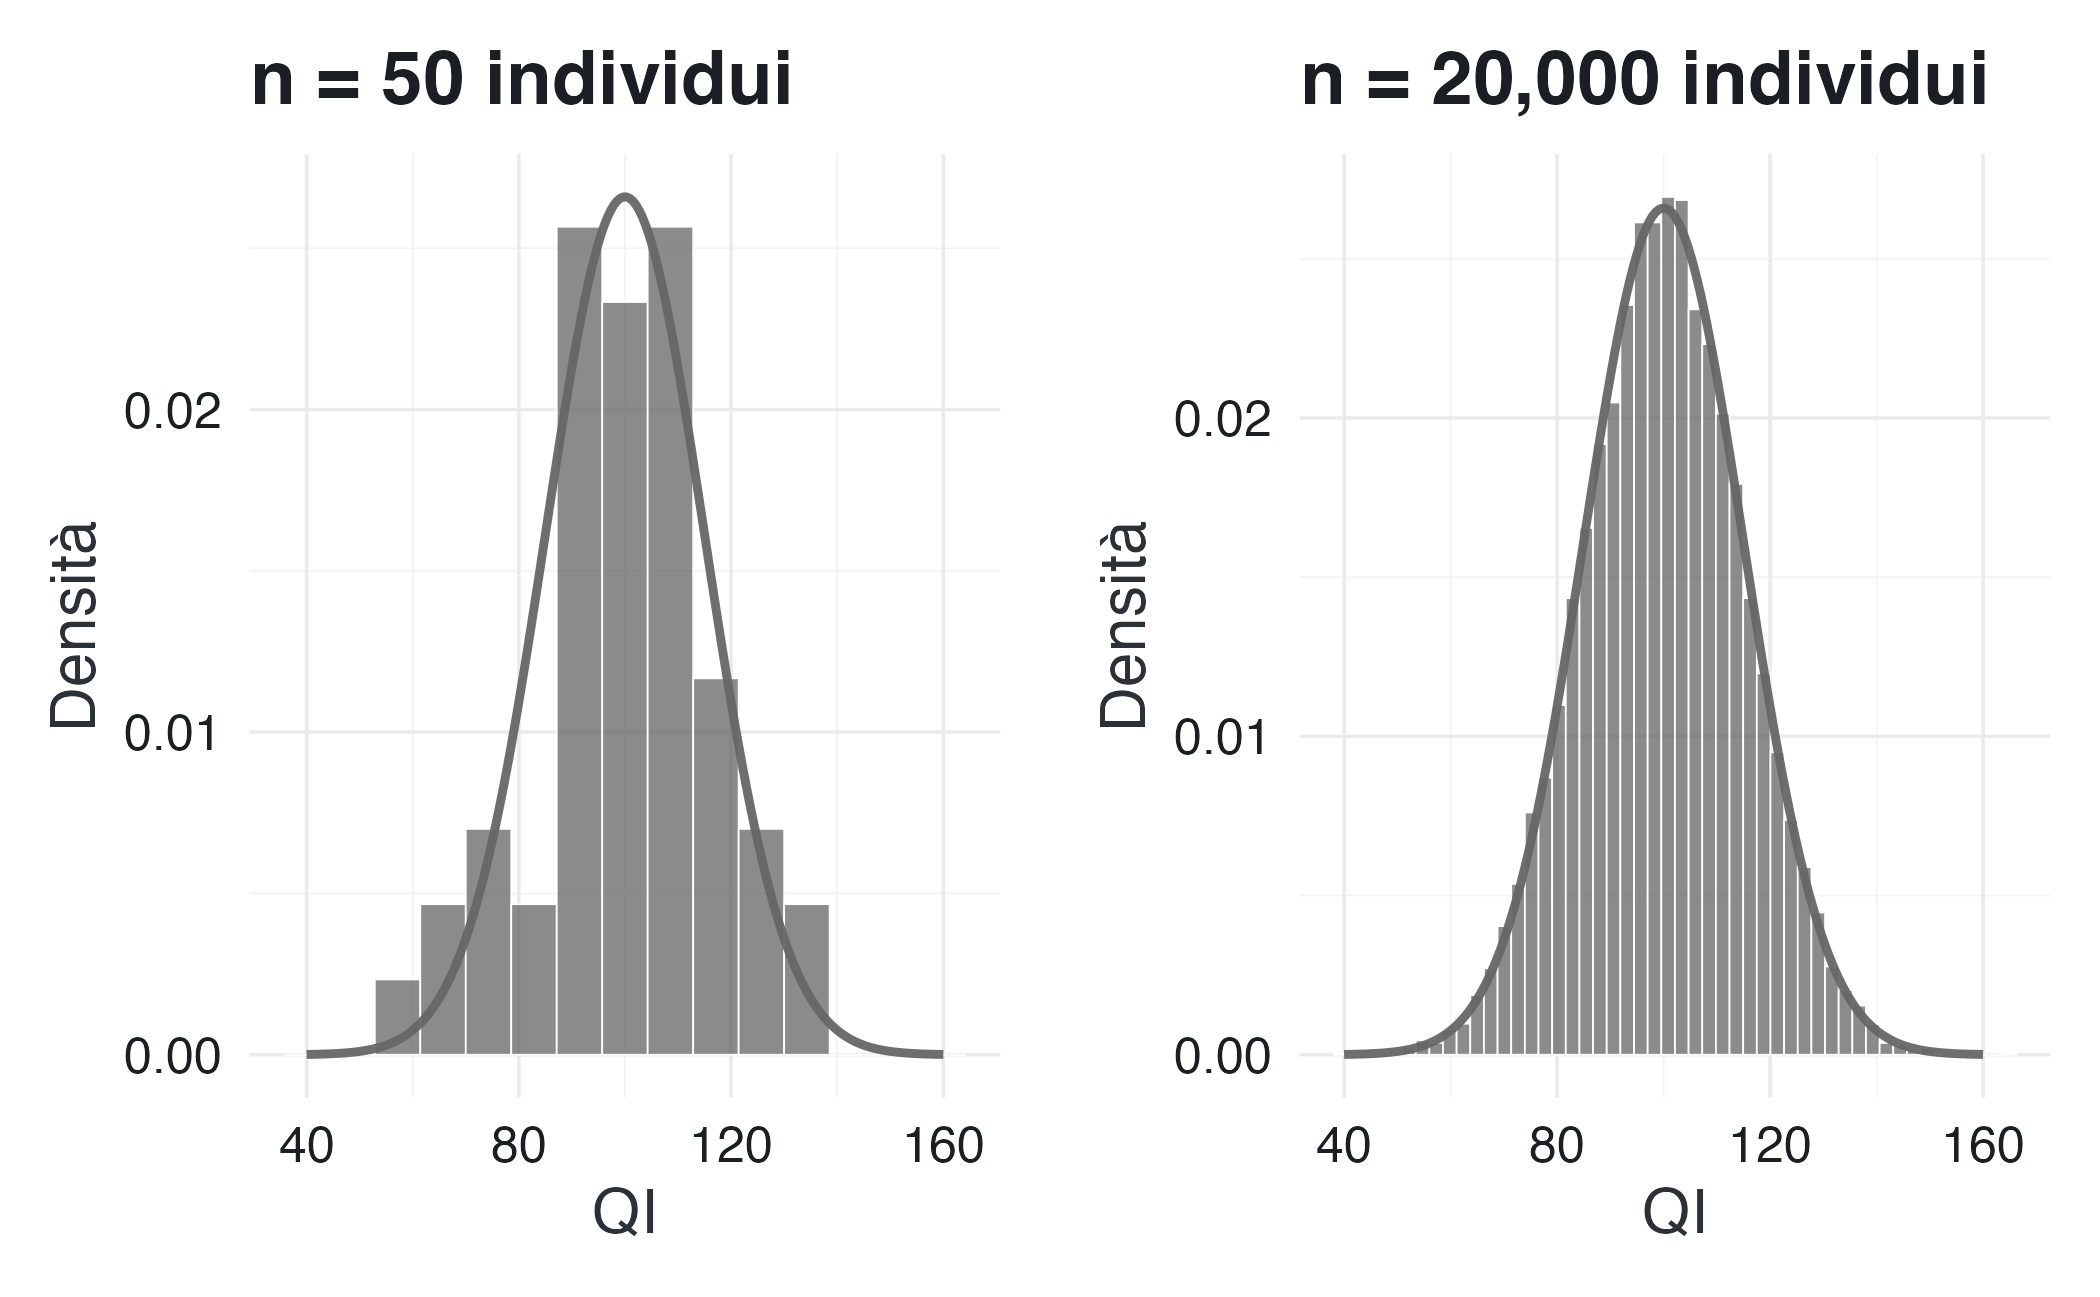
\includegraphics[width=0.85\linewidth,height=\textheight,keepaspectratio]{chapters/probability/07_prob_distributions_files/figure-pdf/unnamed-chunk-3-1.png}
\end{center}

Con soli 50 individui (pannello di sinistra), l'istogramma mostra delle
irregolarità dovute alla variabilità campionaria. Con 20.000 individui
(pannello di destra), l'istogramma aderisce quasi perfettamente alla
curva normale teorica. Questo passaggio dal discreto al continuo mostra
visivamente come la PDF emerga come modello ideale della distribuzione
dei dati nella popolazione.

La PDF non descrive i dettagli di ogni singola osservazione, ma il
\textbf{pattern probabilistico sottostante} che emerge quando si aggrega
un gran numero di dati. Essa rappresenta quindi un \textbf{modello
idealizzato} della popolazione che, sacrificando il rumore individuale,
permette di ottenere un maggiore potere descrittivo, predittivo e
inferenziale.

\subsection{Punto chiave da ricordare}\label{punto-chiave-da-ricordare}

\begin{itemize}
\tightlist
\item
  La PMF assegna probabilità a \textbf{punti}.
\item
  La PDF assegna densità a \textbf{regioni}.
\item
  Solo \textbf{intervalli} hanno probabilità non nulla nel continuo.
\item
  Le densità sono modelli di credenza, non frequenze puntuali.
\end{itemize}

\section{Il paradosso della probabilità
nulla}\label{il-paradosso-della-probabilituxe0-nulla}

Una delle proprietà più controintuitive delle variabili casuali continue
è che la probabilità di osservare \emph{esattamente} un valore specifico
è sempre nulla:

\[
P(X = x_0) = 0 \quad \text{per ogni } x_0 \in \mathbb{R}.
\]

A prima vista, ciò sembra generare un paradosso: se ogni valore puntuale
ha probabilità zero, com'è possibile osservare empiricamente un valore
qualunque? Quando misuriamo un'altezza di 170 cm, non stiamo forse
registrando un evento che la teoria considera impossibile?

\subsection{Perché la probabilità di un punto è
zero}\label{perchuxe9-la-probabilituxe0-di-un-punto-uxe8-zero}

La risposta risiede nel significato geometrico della densità di
probabilità. Per una variabile continua, la probabilità si ottiene come
l'\textbf{area sottostante la curva} su un intervallo. Un singolo punto
corrisponde a un intervallo di ampiezza nulla e, quindi, a un'area
nulla:

\[
P(X = x_0) = \int_{x_0}^{x_0} f_X(x) \, dx = 0.
\]

Questa non è una lacuna della teoria, bensì una proprietà logica del
continuo matematico: qualsiasi area calcolata su un intervallo di
lunghezza zero è necessariamente pari a zero. Se a ogni singolo punto
fosse assegnata una probabilità positiva, l'accumulo su un insieme non
numerabile di punti violerebbe la condizione di normalizzazione, secondo
cui l'area totale sottostante alla densità deve essere pari a 1.

\subsection{Perché allora osserviamo un
valore?}\label{perchuxe9-allora-osserviamo-un-valore}

L'apparente paradosso si dissolve ricordando che una misura empirica non
fornisce mai un punto matematico ``perfetto'', bensì un valore con una
\textbf{risoluzione finita}. Dire ``170 cm'' significa, in pratica, ``un
valore in un piccolo intervallo attorno a 170'', determinato dalla
precisione dello strumento e dal processo di arrotondamento. La teoria
continua descrive proprio questo: le probabilità su intervalli, non su
singoli punti.

\subsection{Implicazioni pratiche}\label{implicazioni-pratiche}

Per le variabili continue non ha senso chiedersi: ``Qual è la
probabilità che il tempo di reazione sia \emph{esattamente} 250 ms?''.
La domanda operativa corretta è: ``Qual è la probabilità che il tempo di
reazione sia compreso tra 245 e 255 ms?''. Le probabilità si calcolano
sempre su \textbf{intervalli}, mai su punti singoli.

Un corollario importante è che, per le variabili continue, includere o
escludere gli estremi di un intervallo non modifica la probabilità:

\[
P(a < X < b) = P(a \leq X < b) = P(a < X \leq b) = P(a \leq X \leq b).
\]

Questo perché i singoli punti \(a\) e \(b\) hanno probabilità zero.

\subsection{Conseguenze per la valutazione
psicologica}\label{conseguenze-per-la-valutazione-psicologica}

Questa proprietà matematica ha implicazioni dirette sull'interpretazione
dei punteggi nei test psicologici. Consideriamo la valutazione del QI:
non ha senso chiedersi ``qual è la probabilità che il QI di questo
bambino sia esattamente 115?'' -- la risposta sarebbe sempre zero, a
prescindere dal bambino.

Le domande clinicamente rilevanti riguardano invece gli intervalli:

\begin{itemize}
\tightlist
\item
  ``Qual è la probabilità che il QI rientri nell'intervallo 110-120?''
  (nella media superiore).
\item
  ``Qual è la probabilità che il QI sia inferiore a 70?'' (soglia per la
  disabilità intellettiva).
\item
  ``Qual è la probabilità che il QI superi 130?'' (soglia per alto
  potenziale).
\end{itemize}

Questo principio si applica a tutte le misurazioni continue in
psicologia: punteggi di ansia, tempi di reazione, livelli di cortisolo e
indici di benessere. La teoria delle variabili continue ci insegna a
formulare le domande nel modo corretto, sempre in termini di intervalli
e mai di valori puntuali.

\section{La funzione di distribuzione
cumulativa}\label{la-funzione-di-distribuzione-cumulativa}

La funzione di distribuzione cumulativa (CDF) fornisce una
rappresentazione unificata delle distribuzioni di probabilità, valida
sia per le variabili discrete che per quelle continue.

\begin{definition}[Funzione di distribuzione
cumulativa]\protect\hypertarget{def-cdf-unified}{}\label{def-cdf-unified}

La \emph{funzione di distribuzione cumulativa} di una variabile casuale
\(X\) è definita come

\[
F_X(x) = P(X \leq x).
\]

\end{definition}

Questa definizione è universale: la CDF ``accumula'' probabilità da
\(-\infty\) fino al valore \(x\), e quantifica la credenza che la
variabile non superi la soglia \(x\).

\subsection{Proprietà fondamentali della
CDF}\label{proprietuxe0-fondamentali-della-cdf}

Ogni CDF soddisfa tre proprietà strutturali.

\begin{theorem}[Proprietà della
CDF]\protect\hypertarget{thm-cdf-properties-detail}{}\label{thm-cdf-properties-detail}

Per qualsiasi variabile casuale \(X\), la CDF \(F_X\) soddisfa:

\begin{enumerate}
\def\labelenumi{\arabic{enumi}.}
\tightlist
\item
  \textbf{Monotonia non decrescente}: se \(a < b\), allora
  \(F_X(a) \leq F_X(b)\).
\item
  \textbf{Limiti agli estremi}: \(\lim_{x \to -\infty} F_X(x) = 0\) e
  \(\lim_{x \to +\infty} F_X(x) = 1\).
\item
  \textbf{Continuità a destra}: \(\lim_{h \to 0^+} F_X(x+h) = F_X(x)\)
  per ogni \(x\).
\end{enumerate}

\end{theorem}

La monotonia riflette l'ovvio: ampliando l'intervallo \((-\infty,x]\)
non si può perdere probabilità. I limiti garantiscono la normalizzazione
globale. La continuità a destra è una convenzione tecnica necessaria
soprattutto per le variabili discrete, in cui la CDF presenta salti.

\subsection{CDF per variabili discrete e
continue}\label{cdf-per-variabili-discrete-e-continue}

Per variabili \textbf{discrete}, la CDF è una funzione a gradini: è
costante tra due valori possibili e cresce a salti. L'altezza del salto
nel punto \(x_i\) è esattamente \(p_X(x_i)\).

Per le variabili \textbf{continue}, invece, la CDF è continua e spesso
derivabile. In questo caso, la densità si ottiene come derivata: \[
f_X(x) = \frac{d}{dx} F_X(x),
\] e reciprocamente la CDF si ottiene integrando la densità: \[
F_X(x) = \int_{-\infty}^{x} f_X(t)\,dt.
\]

\begin{Shaded}
\begin{Highlighting}[]
\CommentTok{\# CDF discreta (soddisfazione lavorativa 1{-}5)}
\NormalTok{valori\_disc }\OtherTok{\textless{}{-}} \DecValTok{1}\SpecialCharTok{:}\DecValTok{5}
\NormalTok{prob\_disc }\OtherTok{\textless{}{-}} \FunctionTok{c}\NormalTok{(}\FloatTok{0.05}\NormalTok{, }\FloatTok{0.10}\NormalTok{, }\FloatTok{0.25}\NormalTok{, }\FloatTok{0.40}\NormalTok{, }\FloatTok{0.20}\NormalTok{)}
\NormalTok{cdf\_disc }\OtherTok{\textless{}{-}} \FunctionTok{cumsum}\NormalTok{(prob\_disc)}

\NormalTok{df\_disc }\OtherTok{\textless{}{-}} \FunctionTok{data.frame}\NormalTok{(}
  \AttributeTok{x\_start =} \FunctionTok{c}\NormalTok{(}\DecValTok{0}\NormalTok{, valori\_disc), }
  \AttributeTok{x\_end =} \FunctionTok{c}\NormalTok{(valori\_disc, }\DecValTok{6}\NormalTok{), }
  \AttributeTok{y =} \FunctionTok{c}\NormalTok{(}\DecValTok{0}\NormalTok{, cdf\_disc)}
\NormalTok{)}

\NormalTok{p1 }\OtherTok{\textless{}{-}} \FunctionTok{ggplot}\NormalTok{() }\SpecialCharTok{+}
  \FunctionTok{geom\_segment}\NormalTok{(}\AttributeTok{data =}\NormalTok{ df\_disc, }\FunctionTok{aes}\NormalTok{(}\AttributeTok{x =}\NormalTok{ x\_start, }\AttributeTok{xend =}\NormalTok{ x\_end, }\AttributeTok{y =}\NormalTok{ y, }\AttributeTok{yend =}\NormalTok{ y),}
               \AttributeTok{linewidth =} \DecValTok{1}\NormalTok{) }\SpecialCharTok{+}
  \FunctionTok{geom\_point}\NormalTok{(}\AttributeTok{data =} \FunctionTok{data.frame}\NormalTok{(}\AttributeTok{x =}\NormalTok{ valori\_disc, }\AttributeTok{y =}\NormalTok{ cdf\_disc),}
             \FunctionTok{aes}\NormalTok{(}\AttributeTok{x =}\NormalTok{ x, }\AttributeTok{y =}\NormalTok{ y), }\AttributeTok{size =} \DecValTok{3}\NormalTok{) }\SpecialCharTok{+}
  \FunctionTok{geom\_point}\NormalTok{(}\AttributeTok{data =} \FunctionTok{data.frame}\NormalTok{(}\AttributeTok{x =}\NormalTok{ valori\_disc, }\AttributeTok{y =} \FunctionTok{c}\NormalTok{(}\DecValTok{0}\NormalTok{, cdf\_disc[}\SpecialCharTok{{-}}\DecValTok{5}\NormalTok{])),}
             \FunctionTok{aes}\NormalTok{(}\AttributeTok{x =}\NormalTok{ x, }\AttributeTok{y =}\NormalTok{ y), }\AttributeTok{size =} \DecValTok{3}\NormalTok{, }\AttributeTok{shape =} \DecValTok{1}\NormalTok{) }\SpecialCharTok{+}
  \FunctionTok{scale\_x\_continuous}\NormalTok{(}\AttributeTok{breaks =} \DecValTok{0}\SpecialCharTok{:}\DecValTok{6}\NormalTok{, }\AttributeTok{limits =} \FunctionTok{c}\NormalTok{(}\DecValTok{0}\NormalTok{, }\DecValTok{6}\NormalTok{)) }\SpecialCharTok{+}
  \FunctionTok{scale\_y\_continuous}\NormalTok{(}\AttributeTok{breaks =} \FunctionTok{seq}\NormalTok{(}\DecValTok{0}\NormalTok{, }\DecValTok{1}\NormalTok{, }\FloatTok{0.2}\NormalTok{)) }\SpecialCharTok{+}
  \FunctionTok{scale\_fill\_qualitative}\NormalTok{() }\SpecialCharTok{+}
  \FunctionTok{labs}\NormalTok{(}\AttributeTok{title =} \StringTok{"CDF discreta (soddisfazione lavorativa)"}\NormalTok{, }
       \AttributeTok{x =} \StringTok{"Livello di soddisfazione"}\NormalTok{, }\AttributeTok{y =} \FunctionTok{expression}\NormalTok{(F[X](x))) }

\CommentTok{\# CDF continua (QI, normale con mu=100, sigma=15)}
\NormalTok{x\_cont }\OtherTok{\textless{}{-}} \FunctionTok{seq}\NormalTok{(}\DecValTok{40}\NormalTok{, }\DecValTok{160}\NormalTok{, }\AttributeTok{length.out =} \DecValTok{200}\NormalTok{)}
\NormalTok{cdf\_cont }\OtherTok{\textless{}{-}} \FunctionTok{pnorm}\NormalTok{(x\_cont, }\AttributeTok{mean =} \DecValTok{100}\NormalTok{, }\AttributeTok{sd =} \DecValTok{15}\NormalTok{)}

\NormalTok{p2 }\OtherTok{\textless{}{-}} \FunctionTok{ggplot}\NormalTok{(}\FunctionTok{data.frame}\NormalTok{(}\AttributeTok{x =}\NormalTok{ x\_cont, }\AttributeTok{y =}\NormalTok{ cdf\_cont), }\FunctionTok{aes}\NormalTok{(}\AttributeTok{x =}\NormalTok{ x, }\AttributeTok{y =}\NormalTok{ y)) }\SpecialCharTok{+}
  \FunctionTok{geom\_line}\NormalTok{(}\AttributeTok{linewidth =} \DecValTok{1}\NormalTok{) }\SpecialCharTok{+}
  \FunctionTok{scale\_y\_continuous}\NormalTok{(}\AttributeTok{breaks =} \FunctionTok{seq}\NormalTok{(}\DecValTok{0}\NormalTok{, }\DecValTok{1}\NormalTok{, }\FloatTok{0.2}\NormalTok{)) }\SpecialCharTok{+}
  \FunctionTok{scale\_fill\_qualitative}\NormalTok{() }\SpecialCharTok{+}
  \FunctionTok{labs}\NormalTok{(}\AttributeTok{title =} \StringTok{"CDF continua (QI)"}\NormalTok{, }
       \AttributeTok{x =} \StringTok{"QI"}\NormalTok{, }\AttributeTok{y =} \FunctionTok{expression}\NormalTok{(F[X](x))) }

\NormalTok{gridExtra}\SpecialCharTok{::}\FunctionTok{grid.arrange}\NormalTok{(p1, p2, }\AttributeTok{ncol =} \DecValTok{2}\NormalTok{)}
\end{Highlighting}
\end{Shaded}

\begin{figure}[H]

\centering{

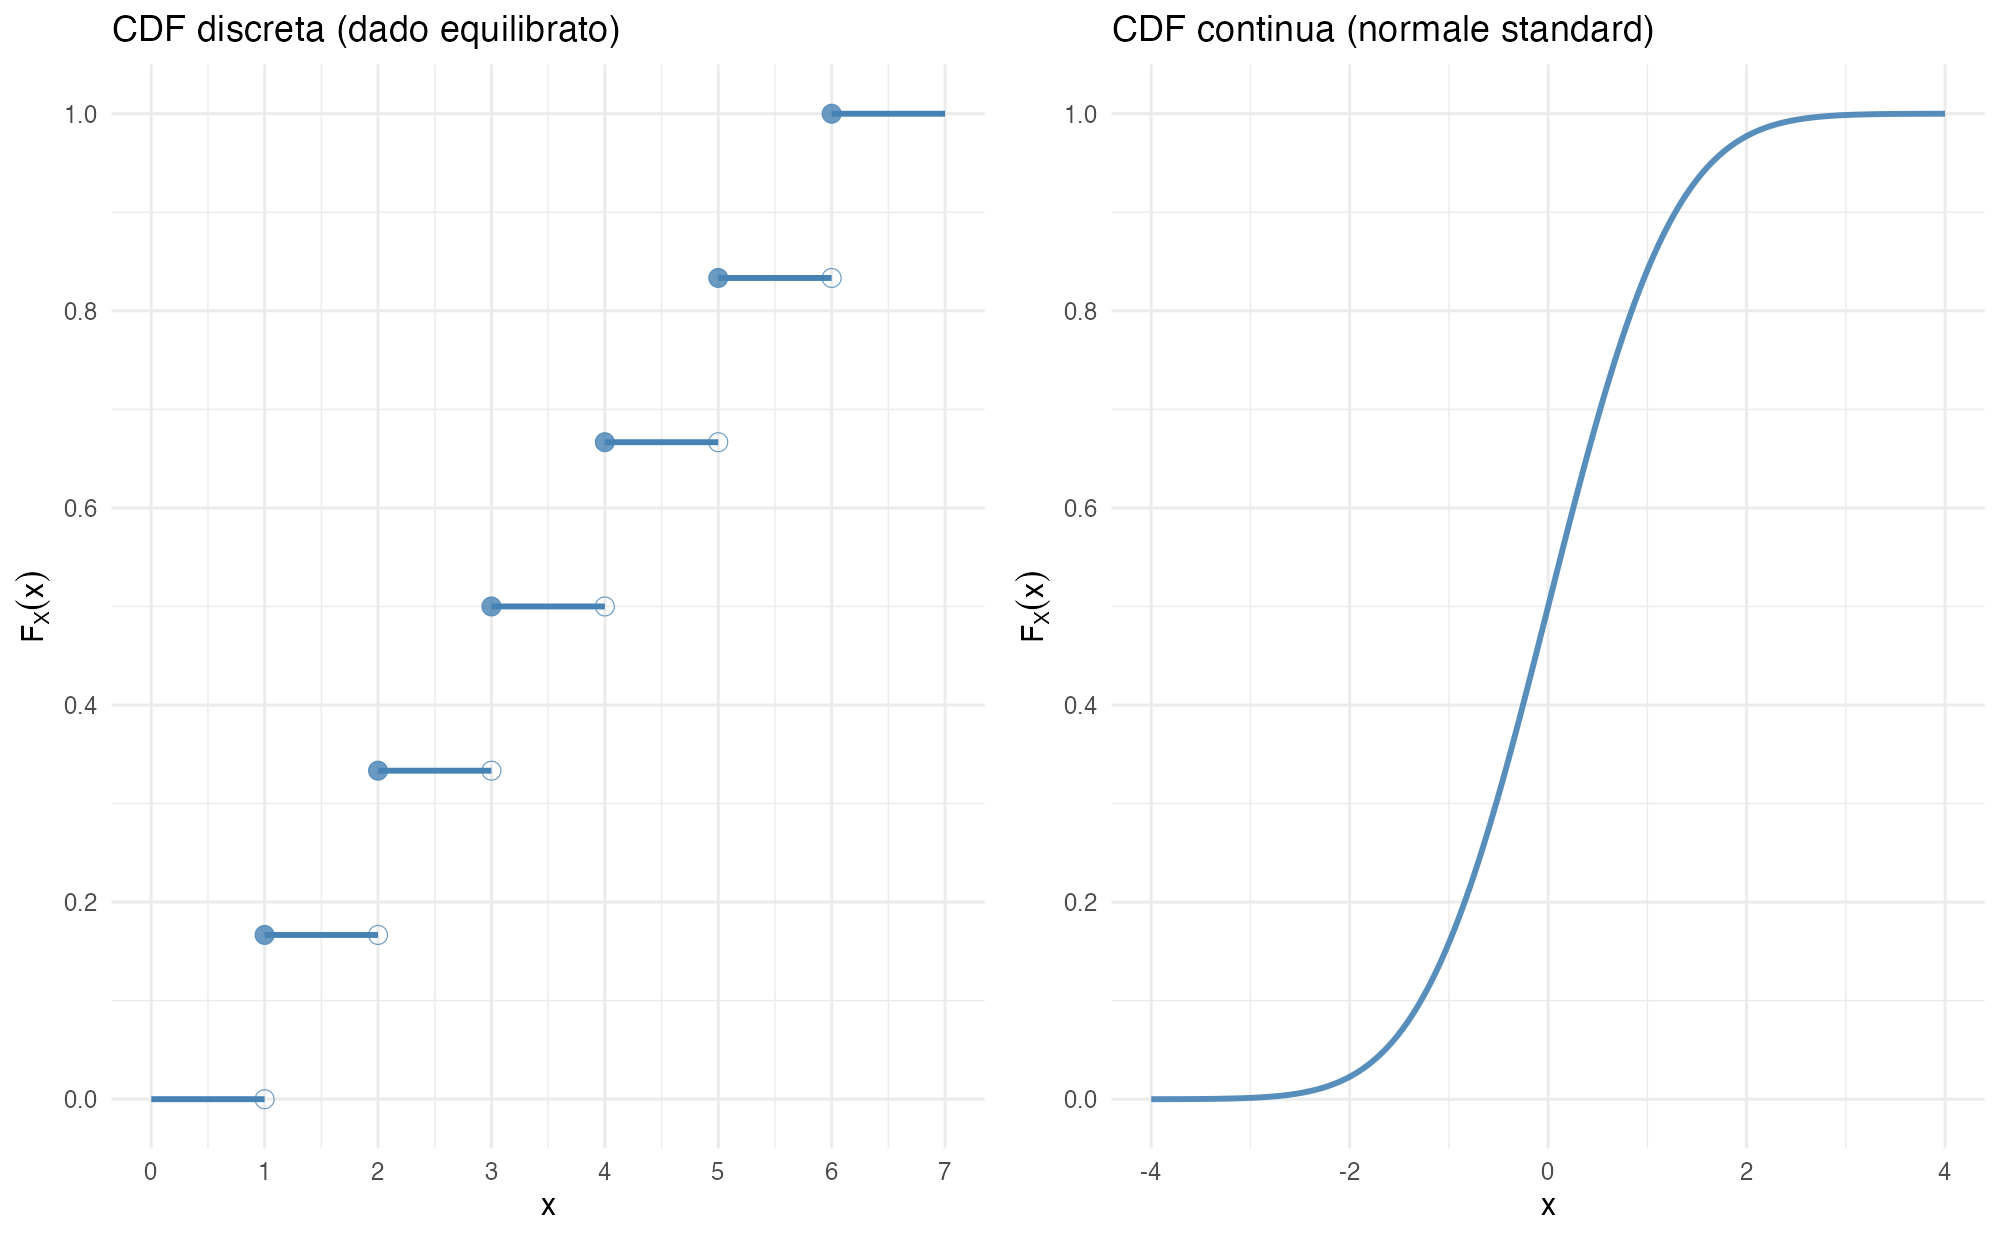
\includegraphics[width=0.85\linewidth,height=\textheight,keepaspectratio]{chapters/probability/07_prob_distributions_files/figure-pdf/fig-cdf-comparison-1.png}

}

\caption{\label{fig-cdf-comparison}CDF di una variabile discreta
(sinistra, a gradini) e di una variabile continua (destra, curva
liscia). Per la variabile discreta, i salti corrispondono ai valori con
massa positiva; per la variabile continua, la CDF è derivabile ovunque.}

\end{figure}%

\subsection{Calcolo di probabilità mediante la
CDF}\label{calcolo-di-probabilituxe0-mediante-la-cdf}

Uno dei principali vantaggi principali della CDF è che permette di
calcolare la probabilità di qualsiasi intervallo come differenza di due
valori: \[
P(a < X \leq b) = F_X(b) - F_X(a).
\] Questa relazione è valida sia per le variabili discrete che per
quelle continue ed è uno strumento computazionale fondamentale in
statistica.

\begin{tcolorbox}[enhanced jigsaw, arc=.35mm, bottomrule=.15mm, bottomtitle=1mm, breakable, colback=white, colbacktitle=quarto-callout-note-color!10!white, colframe=quarto-callout-note-color-frame, coltitle=black, left=2mm, leftrule=.75mm, opacityback=0, opacitybacktitle=0.6, rightrule=.15mm, title=\textcolor{quarto-callout-note-color}{\faInfo}\hspace{0.5em}{Esempio: calcoli con la CDF normale}, titlerule=0mm, toprule=.15mm, toptitle=1mm]

\subsubsection*{Probabilità per la distribuzione del
QI}\label{probabilituxe0-per-la-distribuzione-del-qi}

Consideriamo il quoziente intellettivo (QI) come variabile normale con
media \(\mu = 100\) e deviazione standard \(\sigma = 15\). Calcoliamo
alcune probabilità di interesse clinico.

\begin{Shaded}
\begin{Highlighting}[]
\NormalTok{mu }\OtherTok{\textless{}{-}} \DecValTok{100}
\NormalTok{sigma }\OtherTok{\textless{}{-}} \DecValTok{15}

\CommentTok{\# P(QI \textgreater{} 130) {-} QI molto elevato (gifted)}
\NormalTok{p\_alto }\OtherTok{\textless{}{-}} \DecValTok{1} \SpecialCharTok{{-}} \FunctionTok{pnorm}\NormalTok{(}\DecValTok{130}\NormalTok{, }\AttributeTok{mean =}\NormalTok{ mu, }\AttributeTok{sd =}\NormalTok{ sigma)}
\FunctionTok{cat}\NormalTok{(}\StringTok{"P(QI \textgreater{} 130) ="}\NormalTok{, }\FunctionTok{round}\NormalTok{(p\_alto, }\DecValTok{4}\NormalTok{), }\StringTok{"}\SpecialCharTok{\textbackslash{}n}\StringTok{"}\NormalTok{)}
\CommentTok{\#\textgreater{} P(QI \textgreater{} 130) = 0.0228}

\CommentTok{\# P(85 \textless{} QI \textless{} 115) {-} QI nella norma (±1 SD)}
\NormalTok{p\_norma }\OtherTok{\textless{}{-}} \FunctionTok{pnorm}\NormalTok{(}\DecValTok{115}\NormalTok{, }\AttributeTok{mean =}\NormalTok{ mu, }\AttributeTok{sd =}\NormalTok{ sigma) }\SpecialCharTok{{-}} \FunctionTok{pnorm}\NormalTok{(}\DecValTok{85}\NormalTok{, }\AttributeTok{mean =}\NormalTok{ mu, }\AttributeTok{sd =}\NormalTok{ sigma)}
\FunctionTok{cat}\NormalTok{(}\StringTok{"P(85 \textless{} QI \textless{} 115) ="}\NormalTok{, }\FunctionTok{round}\NormalTok{(p\_norma, }\DecValTok{4}\NormalTok{), }\StringTok{"}\SpecialCharTok{\textbackslash{}n}\StringTok{"}\NormalTok{)}
\CommentTok{\#\textgreater{} P(85 \textless{} QI \textless{} 115) = 0.683}

\CommentTok{\# P(QI \textless{} 70) {-} disabilità intellettiva}
\NormalTok{p\_basso }\OtherTok{\textless{}{-}} \FunctionTok{pnorm}\NormalTok{(}\DecValTok{70}\NormalTok{, }\AttributeTok{mean =}\NormalTok{ mu, }\AttributeTok{sd =}\NormalTok{ sigma)}
\FunctionTok{cat}\NormalTok{(}\StringTok{"P(QI \textless{} 70) ="}\NormalTok{, }\FunctionTok{round}\NormalTok{(p\_basso, }\DecValTok{4}\NormalTok{), }\StringTok{"}\SpecialCharTok{\textbackslash{}n}\StringTok{"}\NormalTok{)}
\CommentTok{\#\textgreater{} P(QI \textless{} 70) = 0.0228}

\CommentTok{\# Percentile 95}
\NormalTok{q95 }\OtherTok{\textless{}{-}} \FunctionTok{qnorm}\NormalTok{(}\FloatTok{0.95}\NormalTok{, }\AttributeTok{mean =}\NormalTok{ mu, }\AttributeTok{sd =}\NormalTok{ sigma)}
\FunctionTok{cat}\NormalTok{(}\StringTok{"95° percentile:"}\NormalTok{, }\FunctionTok{round}\NormalTok{(q95, }\DecValTok{1}\NormalTok{), }\StringTok{"}\SpecialCharTok{\textbackslash{}n}\StringTok{"}\NormalTok{)}
\CommentTok{\#\textgreater{} 95° percentile: 125}
\end{Highlighting}
\end{Shaded}

Questi calcoli mostrano come la CDF (implementata in R da
\texttt{pnorm}) consenta di tradurre le domande cliniche in operazioni
matematiche dirette:

\begin{itemize}
\tightlist
\item
  solo circa il 2.3\% della popolazione ha un QI superiore a 130
  (comunemente utilizzato per definire un ``alto potenziale
  cognitivo'');
\item
  circa il 68\% della popolazione ha un QI compreso tra 85 e 115
  (all'interno di una deviazione standard dalla media);
\item
  circa il 2.3\% ha un QI inferiore a 70 (soglia tradizionale per la
  disabilità intellettiva);
\item
  il 95° percentile corrisponde a un QI di circa 125.
\end{itemize}

\end{tcolorbox}

\section{Interpretazioni bayesiana e
frequentista}\label{interpretazioni-bayesiana-e-frequentista}

Le distribuzioni di probabilità assumono significati diversi nei due
principali paradigmi dell'inferenza statistica. Questa distinzione non è
soltanto filosofica, ma ha un impatto diretto sul modo in cui
interpretiamo i risultati, formuliamo i modelli e comunichiamo
l'incertezza.

\subsection{L'interpretazione
frequentista}\label{linterpretazione-frequentista}

Eccola rivista per migliorare la struttura logica, la precisione
terminologica e il flusso del discorso.

Nel paradigma frequentista, la probabilità è definita come
\textbf{frequenza relativa limite} in una lunga serie ideale di
ripetizioni indipendenti dello stesso esperimento, eseguite in
condizioni identiche. Per un evento del tipo \(a \leq X \leq b\), questa
interpretazione implica:

\[
P(a \leq X \leq b) = \lim_{n \to \infty} \frac{\#\{X_i \in [a,b]\}}{n},
\] dove \(X_1, X_2, \ldots, X_n\) sono realizzazioni indipendenti dello
stesso processo stocastico.

In questa prospettiva, la funzione di densità (PDF) non è una misura di
credenza soggettiva, ma una \textbf{descrizione del meccanismo
generativo dei dati}: essa rappresenta la forma limite alla quale
converge l'istogramma delle osservazioni man mano che il campione si
espande e gli intervalli di classizzazione diventano arbitrariamente
fini. La variabile casuale \(X\) modella l'esito di un esperimento
ripetibile, e la sua PDF descrive la variabilità osservabile
\textbf{tra} le diverse ripetizioni.

Un esempio classico è la distribuzione dell'altezza nella popolazione
adulta. Un modello normale con media \(\mu = 170\) cm e deviazione
standard \(\sigma = 10\) cm descrive quale proporzione di individui ci
aspetteremmo di osservare in ogni intervallo di altezza, se potessimo
campionare ripetutamente e a caso da una popolazione di riferimento
molto ampia e stabile.

\subsection{L'interpretazione
bayesiana}\label{linterpretazione-bayesiana}

Nel paradigma bayesiano, la probabilità quantifica un \textbf{grado di
credenza razionale}, ovvero una misura della plausibilità assegnata a
diverse possibilità alla luce delle informazioni disponibili. Non è
necessario immaginare delle ripetizioni ipotetiche: la probabilità è una
proprietà dello stato informativo dell'osservatore.

\begin{definition}[Interpretazione bayesiana della
PDF]\protect\hypertarget{def-bayesian-pdf}{}\label{def-bayesian-pdf}

Dal punto di vista bayesiano, la funzione di densità \(f_X(x)\)
rappresenta la \textbf{distribuzione della nostra incertezza} sul valore
di una quantità \(X\), che è considerata fissa ma ignota. L'integrale
\(\int_a^b f_X(x)\,dx\) non misura una frequenza, ma il \textbf{grado di
credenza} che il valore effettivo di \(X\) appartenga all'intervallo
\([a,b]\).

\end{definition}

Ne deriva un'implicazione cruciale: il paradigma bayesiano permette di
descrivere con distribuzioni di probabilità non solo i dati osservabili,
ma anche quelle quantità che nel frequentismo sono considerate parametri
fissi, come l'effetto medio di un trattamento, la prevalenza di una
malattia o la probabilità soggettiva di risposta alla terapia.

In questa logica, una funzione di densità bayesiana rappresenta una
mappa di plausibilità: le regioni con densità più alta corrispondono a
valori che riteniamo più credibili, mentre quelle con densità bassa
riflettono ipotesi meno plausibili. La forma stessa della distribuzione,
la sua simmetria o asimmetria, l'estensione delle code e il grado di
concentrazione esprimono esplicitamente ciò che sappiamo e, soprattutto,
ciò che ignoriamo sulla quantità di interesse.

\subsection{Confronto tra le due
prospettive}\label{confronto-tra-le-due-prospettive}

Le differenze metodologiche emergono in modo netto in un esempio
elementare. Supponiamo di voler stimare l'altezza media di una
popolazione, denotata con \(\theta\).

\begin{itemize}
\item
  \textbf{Nel paradigma frequentista}, \(\theta\) è un \textbf{parametro
  fisso ma sconosciuto}. La probabilità si applica alle statistiche
  calcolate dai campioni, come la media campionaria \(\bar{X}\). La PDF
  di \(\bar{X}\) descrive come quest'ultima varierebbe se ripetessimo
  infinite volte il campionamento dalla stessa popolazione. Di
  conseguenza, un intervallo di confidenza al 95\% \textbf{non} afferma
  che il valore di \(\theta\) abbia una probabilità dello 0.95 di cadere
  in quell'intervallo (dal momento che \(\theta\) non è una variabile
  casuale), ma piuttosto che il \emph{metodo} utilizzato per costruire
  l'intervallo lo conterrebbe nel 95\% delle ripetizioni sperimentali.
\item
  \textbf{Nel paradigma bayesiano}, invece, è possibile assegnare
  direttamente una distribuzione di probabilità a \(\theta\),
  quantificando la nostra incertezza su di esso. La distribuzione
  \emph{a priori} formalizza le conoscenze iniziali, mentre quella
  \emph{a posteriori} aggiorna tali conoscenze con le informazioni
  provenienti dai dati. Pertanto, un intervallo di credibilità al 95\%
  dichiara esattamente ciò che suggerisce: alla luce dei dati osservati
  e della prior, la probabilità soggettiva che il valore di \(\theta\)
  si trovi in quell'intervallo è 0.95.
\end{itemize}

\begin{Shaded}
\begin{Highlighting}[]
\FunctionTok{set.seed}\NormalTok{(}\DecValTok{123}\NormalTok{)}

\CommentTok{\# Frequentista: distribuzione dei dati}
\NormalTok{x\_freq }\OtherTok{\textless{}{-}} \FunctionTok{rnorm}\NormalTok{(}\DecValTok{1000}\NormalTok{, }\AttributeTok{mean =} \DecValTok{170}\NormalTok{, }\AttributeTok{sd =} \DecValTok{10}\NormalTok{)}
\NormalTok{x\_seq }\OtherTok{\textless{}{-}} \FunctionTok{seq}\NormalTok{(}\DecValTok{140}\NormalTok{, }\DecValTok{200}\NormalTok{, }\AttributeTok{length.out =} \DecValTok{200}\NormalTok{)}
\NormalTok{y\_teorica }\OtherTok{\textless{}{-}} \FunctionTok{dnorm}\NormalTok{(x\_seq, }\AttributeTok{mean =} \DecValTok{170}\NormalTok{, }\AttributeTok{sd =} \DecValTok{10}\NormalTok{)}

\NormalTok{p1 }\OtherTok{\textless{}{-}} \FunctionTok{ggplot}\NormalTok{() }\SpecialCharTok{+}
  \FunctionTok{geom\_histogram}\NormalTok{(}\AttributeTok{data =} \FunctionTok{data.frame}\NormalTok{(}\AttributeTok{x =}\NormalTok{ x\_freq), }\FunctionTok{aes}\NormalTok{(}\AttributeTok{x =}\NormalTok{ x, }\AttributeTok{y =} \FunctionTok{after\_stat}\NormalTok{(density)),}
                 \AttributeTok{bins =} \DecValTok{30}\NormalTok{, }\AttributeTok{alpha =} \FloatTok{0.5}\NormalTok{, }\AttributeTok{color =} \StringTok{"white"}\NormalTok{) }\SpecialCharTok{+}
  \FunctionTok{geom\_line}\NormalTok{(}\AttributeTok{data =} \FunctionTok{data.frame}\NormalTok{(}\AttributeTok{x =}\NormalTok{ x\_seq, }\AttributeTok{y =}\NormalTok{ y\_teorica), }
            \FunctionTok{aes}\NormalTok{(}\AttributeTok{x =}\NormalTok{ x, }\AttributeTok{y =}\NormalTok{ y), }\AttributeTok{linewidth =} \FloatTok{1.2}\NormalTok{) }\SpecialCharTok{+}
  \FunctionTok{scale\_fill\_qualitative}\NormalTok{() }\SpecialCharTok{+}
  \FunctionTok{labs}\NormalTok{(}\AttributeTok{title =} \StringTok{"Frequentista:}\SpecialCharTok{\textbackslash{}n}\StringTok{distribuzione dei dati"}\NormalTok{,}
       \AttributeTok{subtitle =} \StringTok{"PDF come istogramma limite di ripetizioni"}\NormalTok{,}
       \AttributeTok{x =} \StringTok{"Altezza (cm)"}\NormalTok{, }\AttributeTok{y =} \StringTok{"Densità"}\NormalTok{) }

\CommentTok{\# Bayesiano: distribuzione della credenza su un parametro}
\NormalTok{theta\_seq }\OtherTok{\textless{}{-}} \FunctionTok{seq}\NormalTok{(}\DecValTok{165}\NormalTok{, }\DecValTok{175}\NormalTok{, }\AttributeTok{length.out =} \DecValTok{200}\NormalTok{)}
\NormalTok{prior }\OtherTok{\textless{}{-}} \FunctionTok{dnorm}\NormalTok{(theta\_seq, }\AttributeTok{mean =} \DecValTok{170}\NormalTok{, }\AttributeTok{sd =} \DecValTok{2}\NormalTok{)}

\NormalTok{p2 }\OtherTok{\textless{}{-}} \FunctionTok{ggplot}\NormalTok{() }\SpecialCharTok{+}
  \FunctionTok{geom\_ribbon}\NormalTok{(}\AttributeTok{data =} \FunctionTok{data.frame}\NormalTok{(}\AttributeTok{x =}\NormalTok{ theta\_seq, }\AttributeTok{y =}\NormalTok{ prior),}
              \FunctionTok{aes}\NormalTok{(}\AttributeTok{x =}\NormalTok{ x, }\AttributeTok{ymin =} \DecValTok{0}\NormalTok{, }\AttributeTok{ymax =}\NormalTok{ y), }
              \AttributeTok{alpha =} \FloatTok{0.3}\NormalTok{) }\SpecialCharTok{+}
  \FunctionTok{geom\_line}\NormalTok{(}\AttributeTok{data =} \FunctionTok{data.frame}\NormalTok{(}\AttributeTok{x =}\NormalTok{ theta\_seq, }\AttributeTok{y =}\NormalTok{ prior),}
            \FunctionTok{aes}\NormalTok{(}\AttributeTok{x =}\NormalTok{ x, }\AttributeTok{y =}\NormalTok{ y), }\AttributeTok{linewidth =} \FloatTok{1.2}\NormalTok{) }\SpecialCharTok{+}
  \FunctionTok{geom\_point}\NormalTok{(}\FunctionTok{aes}\NormalTok{(}\AttributeTok{x =} \DecValTok{170}\NormalTok{, }\AttributeTok{y =} \DecValTok{0}\NormalTok{), }\AttributeTok{size =} \DecValTok{3}\NormalTok{, }\AttributeTok{color =} \StringTok{"black"}\NormalTok{) }\SpecialCharTok{+}
  \FunctionTok{annotate}\NormalTok{(}\StringTok{"text"}\NormalTok{, }\AttributeTok{x =} \DecValTok{170}\NormalTok{, }\AttributeTok{y =} \SpecialCharTok{{-}}\FloatTok{0.02}\NormalTok{, }\AttributeTok{label =} \StringTok{"θ (valore vero ignoto)"}\NormalTok{, }\AttributeTok{size =} \DecValTok{3}\NormalTok{) }\SpecialCharTok{+}
  \FunctionTok{scale\_fill\_qualitative}\NormalTok{() }\SpecialCharTok{+}
  \FunctionTok{labs}\NormalTok{(}\AttributeTok{title =} \StringTok{"Bayesiano:}\SpecialCharTok{\textbackslash{}n}\StringTok{distribuzione della credenza"}\NormalTok{,}
       \AttributeTok{subtitle =} \StringTok{"PDF come mappa di plausibilità sul parametro"}\NormalTok{,}
       \AttributeTok{x =} \FunctionTok{expression}\NormalTok{(theta }\SpecialCharTok{\textasciitilde{}} \StringTok{"(altezza media)"}\NormalTok{), }\AttributeTok{y =} \StringTok{"Densità"}\NormalTok{) }

\NormalTok{gridExtra}\SpecialCharTok{::}\FunctionTok{grid.arrange}\NormalTok{(p1, p2, }\AttributeTok{ncol =} \DecValTok{2}\NormalTok{)}
\end{Highlighting}
\end{Shaded}

\begin{figure}[H]

\centering{

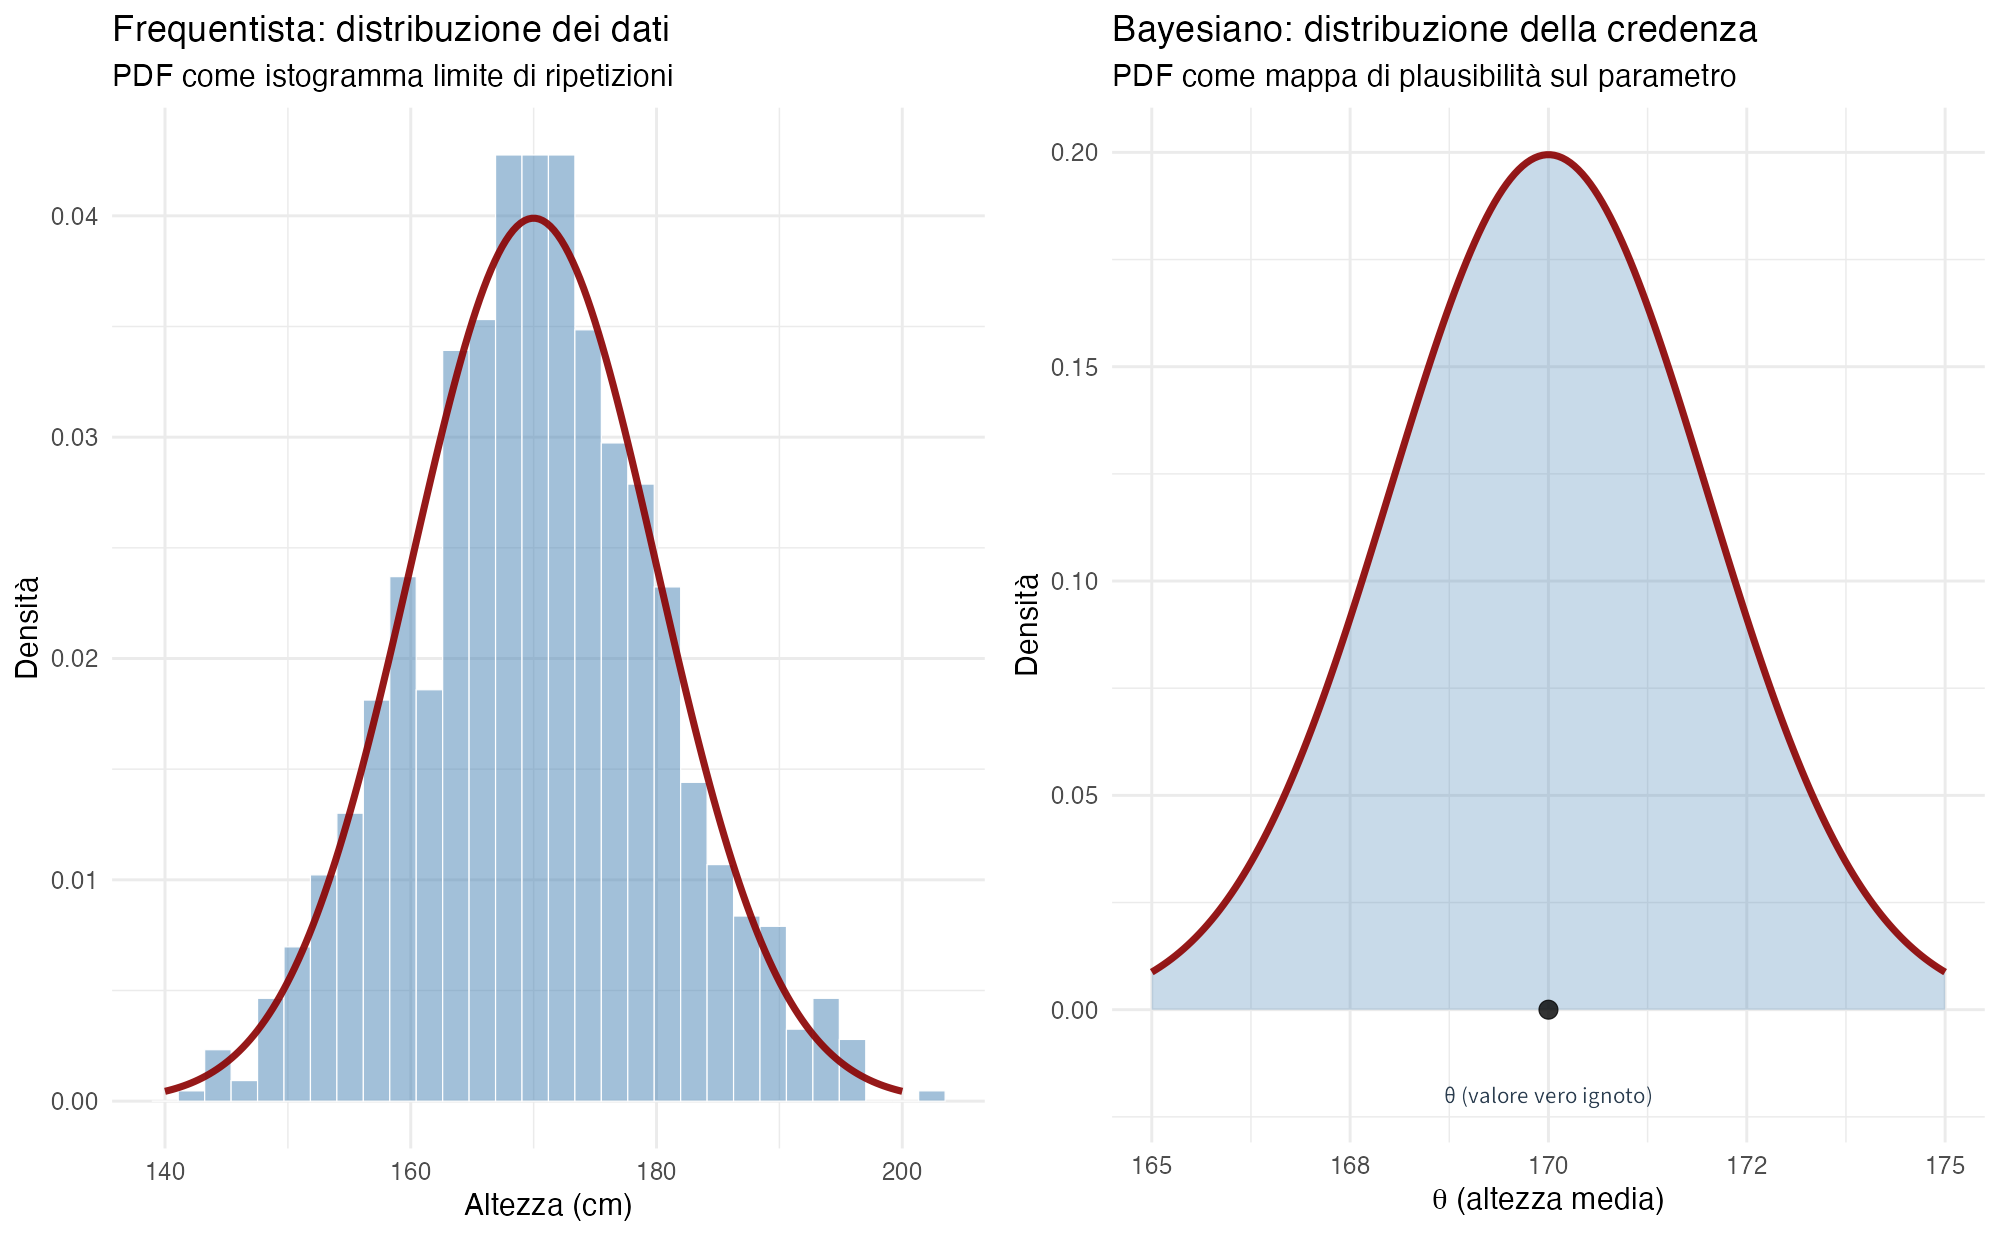
\includegraphics[width=0.85\linewidth,height=\textheight,keepaspectratio]{chapters/probability/07_prob_distributions_files/figure-pdf/fig-freq-vs-bayes-1.png}

}

\caption{\label{fig-freq-vs-bayes}Confronto tra interpretazioni
frequentista e bayesiana. A sinistra: la PDF descrive la distribuzione
dei dati (istogramma) in ripetizioni dell'esperimento. A destra: la PDF
rappresenta la credenza sul valore di un parametro, con l'incertezza
`spalmata' sui valori possibili.}

\end{figure}%

La CDF rimane in entrambi i paradigmi lo strumento fondamentale per
calcolare le probabilità degli intervalli. A cambiare è \textbf{il
significato} che attribuiamo a queste probabilità: nel paradigma
frequentista essa rappresenta una \textbf{frequenza limite} di un evento
su ripetizioni ideali dell'esperimento; nel paradigma bayesiana, essa
esprime il \textbf{grado di credenza} soggettiva che una proposizione
sia vera, sulla base delle informazioni disponibili.

\section*{Riflessioni conclusive}\label{riflessioni-conclusive-6}

\markright{Riflessioni conclusive}

La distinzione tra \textbf{massa} e \textbf{densità} di probabilità
evidenzia una differenza strutturale fondamentale tra variabili casuali
discrete e continue. Per le variabili casuali discrete, la probabilità è
concentrata in punti isolati, mentre per quelle continue è distribuita
in modo continuo e misurabile solo integrando su intervalli di valori.

Il cosiddetto ``paradosso'' della probabilità nulla per punti esatti
nelle distribuzioni continue si dissolve quando si riconosce che, in
questo ambito, la probabilità è intrinsecamente una proprietà degli
\textbf{intervalli}, non dei \textbf{punti}. Ogni singolo valore
contribuisce con probabilità nulla, ma l'integrazione su un continuum di
valori produce quantità probabilisticamente significative. Per lo
psicologo, ciò si traduce in una prassi operativa: formulare domande
come ``Qual è la probabilità che il punteggio cada in \emph{questo
intervallo}?'', anziché chiedersi ``Qual è la probabilità di ottenere
\emph{esattamente questo} punteggio?''.

In questo contesto, la \textbf{funzione di distribuzione cumulativa}
(CDF) si rivela uno strumento unificante. Essa offre una
rappresentazione coerente delle distribuzioni sia per variabili discrete
che continue, consente il calcolo diretto delle probabilità su
intervalli arbitrari e chiarisce sistematicamente il legame tra la
funzione di massa, la funzione di densità e le probabilità osservabili.

Infine, la differenza tra l'interpretazione \textbf{frequentista} e
\textbf{bayesiana} delle distribuzioni non è un dibattito puramente
filosofico, ma implica scelte metodologiche concrete nella costruzione e
nell'interpretazione dei modelli statistici. Poiché l'obiettivo di
questo corso è l'inferenza in condizioni di incertezza, ci concentreremo
sul paradigma bayesiano, il cui formalismo è appositamente concepito per
rappresentare, e aggiornare in modo logicamente coerente, lo stato delle
nostre conoscenze alla luce dell'evidenza empirica.

\section*{Punti chiave da ricordare}\label{punti-chiave-da-ricordare-6}
\addcontentsline{toc}{section}{Punti chiave da ricordare}

\markright{Punti chiave da ricordare}

\begin{tcolorbox}[enhanced jigsaw, arc=.35mm, bottomrule=.15mm, bottomtitle=1mm, breakable, colback=white, colbacktitle=quarto-callout-important-color!10!white, colframe=quarto-callout-important-color-frame, coltitle=black, left=2mm, leftrule=.75mm, opacityback=0, opacitybacktitle=0.6, rightrule=.15mm, title=\textcolor{quarto-callout-important-color}{\faExclamation}\hspace{0.5em}{Importante}, titlerule=0mm, toprule=.15mm, toptitle=1mm]

\textbf{Concetti essenziali di questo capitolo:}

\begin{enumerate}
\def\labelenumi{\arabic{enumi}.}
\tightlist
\item
  \textbf{Massa vs densità: due modi profondamente diversi di
  distribuire probabilità}

  \begin{itemize}
  \tightlist
  \item
    \textbf{Massa (PMF)}: probabilità concentrata in punti discreti,
    come ``pesi'' su una bilancia.
  \item
    \textbf{Densità (PDF)}: probabilità distribuita su un continuum,
    come massa in un fluido.
  \item
    La distinzione non è solo tecnica ma riflette strutture matematiche
    diverse (somme vs integrali).
  \end{itemize}
\item
  \textbf{La PMF assegna probabilità dirette a valori specifici}

  \begin{itemize}
  \tightlist
  \item
    \(p_X(x) = P(X = x)\) è la probabilità \emph{del} punto \(x\).
  \item
    Diagramma a barre: l'altezza rappresenta direttamente la
    probabilità.
  \item
    Somma delle probabilità: \(\sum_x p_X(x) = 1\).
  \end{itemize}
\item
  \textbf{La PDF misura concentrazione locale, non probabilità diretta}

  \begin{itemize}
  \tightlist
  \item
    \(f_X(x)\) indica ``quanta probabilità c'è per unità di lunghezza''
    attorno a \(x\).
  \item
    \(f_X(x)\) può essere maggiore di 1 (non è una probabilità!).
  \item
    Probabilità tramite integrazione:
    \(P(a \leq X \leq b) = \int_a^b f_X(x) \, dx\).
  \end{itemize}
\item
  \textbf{Il ``paradosso'' P(X = x) = 0 per variabili continue}

  \begin{itemize}
  \tightlist
  \item
    Non è un paradosso: un singolo punto ha ``misura zero'' nel
    continuo.
  \item
    Come la ``massa di un punto'' in un filo: zero, ma il punto esiste.
  \item
    Differenza cruciale: probabilità zero ≠ impossibilità logica.
  \item
    Solo intervalli (anche infinitesimi) hanno probabilità positiva.
  \end{itemize}
\item
  \textbf{Dagli istogrammi alle densità: il limite continuo}

  \begin{itemize}
  \tightlist
  \item
    All'aumentare di \(n\) e al diminuire della larghezza dei bin, gli
    istogrammi convergono alla PDF.
  \item
    La PDF è il limite ideale quando bin → 0 e \(n\) → ∞.
  \item
    Illustra visivamente come la densità emerga naturalmente dai dati.
  \end{itemize}
\item
  \textbf{CDF come rappresentazione unificata}

  \begin{itemize}
  \tightlist
  \item
    \(F_X(x) = P(X \leq x)\) vale sia per discrete che per continue.
  \item
    Discrete: funzione a gradini con salti in corrispondenza dei valori
    possibili.
  \item
    Continue: funzione liscia e crescente.
  \item
    Proprietà universali: monotona non decrescente, \(F(-\infty) = 0\),
    \(F(+\infty) = 1\).
  \end{itemize}
\item
  \textbf{Interpretazioni bayesiana vs frequentista delle distribuzioni}

  \begin{itemize}
  \tightlist
  \item
    \textbf{Frequentista}: la PDF descrive il comportamento dei dati in
    ripetizioni ipotetiche.
  \item
    \textbf{Bayesiano}: la PDF rappresenta il grado di credenza sui
    possibili valori (anche parametri!).
  \item
    Stessa forma matematica, interpretazione epistemica profondamente
    diversa.
  \item
    Per il bayesiano, distribuzioni di parametri sono naturali; per il
    frequentista no.
  \end{itemize}
\end{enumerate}

\textbf{Formule da ricordare:}

\textbf{PMF (discrete):} \[
p_X(x) = P(X = x), \quad \sum_{x} p_X(x) = 1
\]

\textbf{PDF (continue):} \[
P(a \leq X \leq b) = \int_a^b f_X(x) \, dx, \quad \int_{-\infty}^{+\infty} f_X(x) \, dx = 1
\]

\textbf{CDF (universale):} \[
F_X(x) = P(X \leq x) = \begin{cases}
\sum_{x_i \leq x} p_X(x_i) & \text{(discreta)} \\
\int_{-\infty}^x f_X(t) \, dt & \text{(continua)}
\end{cases}
\]

\textbf{Relazione PDF-CDF per variabili continue:} \[
f_X(x) = \frac{d}{dx} F_X(x) \quad \text{(la densità è la derivata della CDF)}
\]

\textbf{Calcolo di probabilità da CDF:} \[
P(a \leq X \leq b) = F_X(b) - F_X(a)
\]

\textbf{Proprietà chiave:}

\begin{itemize}
\tightlist
\item
  \textbf{Discrete}: \(P(X = x) = p_X(x) > 0\) è possibile.
\item
  \textbf{Continue}: \(P(X = x) = 0\) sempre (ma \(f_X(x)\) può essere
  \textgreater{} 0).
\item
  \textbf{PDF può essere \textgreater{} 1}: non è una probabilità ma una
  densità!
\item
  \textbf{CDF sempre ∈ {[}0,1{]}}: rappresenta una probabilità
  cumulativa.
\end{itemize}

\textbf{Per il prossimo capitolo:}

Nel Capitolo~\ref{sec-prob-random-var-properties} le \textbf{proprietà
delle variabili casuali}: valore atteso (centro di gravità
probabilistico), varianza (dispersione), e le loro proprietà algebriche.
Questi strumenti di sintesi ci permetteranno di caratterizzare
distribuzioni complesse con pochi numeri e di propagare l'incertezza
attraverso trasformazioni matematiche, preparando il terreno per
l'inferenza bayesiana parametrica.

\end{tcolorbox}

\begin{tcolorbox}[enhanced jigsaw, arc=.35mm, bottomrule=.15mm, bottomtitle=1mm, breakable, colback=white, colbacktitle=quarto-callout-important-color!10!white, colframe=quarto-callout-important-color-frame, coltitle=black, left=2mm, leftrule=.75mm, opacityback=0, opacitybacktitle=0.6, rightrule=.15mm, title=\textcolor{quarto-callout-important-color}{\faExclamation}\hspace{0.5em}{Esercizi}, titlerule=0mm, toprule=.15mm, toptitle=1mm]

\subsection*{Esercizi concettuali}\label{esercizi-concettuali-1}

\begin{enumerate}
\def\labelenumi{\arabic{enumi}.}
\item
  Spiega perché il termine ``massa'' è appropriato per le distribuzioni
  discrete e ``densità'' per quelle continue. Quale proprietà fisica
  richiamano queste metafore?
\item
  Un collega afferma: ``Se \(P(X = 170) = 0\), allora è impossibile
  osservare \(X = 170\).'' Correggi questo fraintendimento e spiega la
  distinzione tra ``probabilità zero'' e ``impossibilità''.
\item
  Nel paradigma bayesiano, ha senso assegnare una distribuzione di
  probabilità a una costante fisica come la velocità della luce? Perché
  sì o perché no?
\end{enumerate}

\subsection*{Esercizi sulla PMF}\label{esercizi-sulla-pmf}

\begin{enumerate}
\def\labelenumi{\arabic{enumi}.}
\setcounter{enumi}{3}
\item
  Un test psicometrico produce punteggi interi da 1 a 5 secondo la
  distribuzione:

  {\def\LTcaptype{none} % do not increment counter
  \begin{longtable}[]{@{}cccccc@{}}
  \toprule\noalign{}
  Punteggio & 1 & 2 & 3 & 4 & 5 \\
  \midrule\noalign{}
  \endhead
  \bottomrule\noalign{}
  \endlastfoot
  \(p_X(x)\) & 0.10 & 0.20 & 0.35 & 0.25 & 0.10 \\
  \end{longtable}
  }

  \begin{enumerate}
  \def\labelenumii{\alph{enumii}.}
  \tightlist
  \item
    Calcola \(P(X \geq 3)\).
  \item
    Calcola \(P(2 \leq X \leq 4)\).
  \item
    Calcola il valore atteso \(\mathbb{E}[X]\).
  \item
    Costruisci la CDF e rappresentala graficamente.
  \end{enumerate}
\item
  Nella scala LSNS-6 (Lubben Social Network Scale), il numero di amici
  intimi segue approssimativamente questa distribuzione:

  {\def\LTcaptype{none} % do not increment counter
  \begin{longtable}[]{@{}ccccccc@{}}
  \toprule\noalign{}
  Amici & 0 & 1 & 2 & 3 & 4 & 5+ \\
  \midrule\noalign{}
  \endhead
  \bottomrule\noalign{}
  \endlastfoot
  \(p_X(x)\) & 0.05 & 0.15 & 0.25 & 0.30 & 0.15 & 0.10 \\
  \end{longtable}
  }

  \begin{enumerate}
  \def\labelenumii{\alph{enumii}.}
  \tightlist
  \item
    Qual è la probabilità di avere almeno 3 amici intimi?
  \item
    Qual è la probabilità di avere meno di 2 amici intimi?
  \item
    Calcola valore atteso e varianza.
  \end{enumerate}
\end{enumerate}

\subsection*{Esercizi sulla PDF e CDF}\label{esercizi-sulla-pdf-e-cdf}

\begin{enumerate}
\def\labelenumi{\arabic{enumi}.}
\setcounter{enumi}{5}
\item
  Il punteggio alla Satisfaction with Life Scale (SWLS) può essere
  approssimato da una distribuzione normale con \(\mu = 20\) e
  \(\sigma = 5\).

  \begin{enumerate}
  \def\labelenumii{\alph{enumii}.}
  \tightlist
  \item
    Qual è la probabilità di un punteggio superiore a 25?
  \item
    Qual è la probabilità di un punteggio tra 15 e 25?
  \item
    Quale punteggio delimita il 10\% superiore della distribuzione?
  \item
    Verifica i calcoli con le funzioni R \texttt{pnorm} e
    \texttt{qnorm}.
  \end{enumerate}
\item
  Il tempo di reazione in un compito cognitivo segue una distribuzione
  normale con \(\mu = 350\) ms e \(\sigma = 50\) ms.

  \begin{enumerate}
  \def\labelenumii{\alph{enumii}.}
  \tightlist
  \item
    Qual è la probabilità che un tempo di reazione sia inferiore a 300
    ms?
  \item
    Entro quale intervallo simmetrico attorno alla media cade il 95\%
    dei tempi?
  \item
    Un tempo di 450 ms è ``anomalo''? Calcola la probabilità di
    osservare un tempo così estremo o più.
  \end{enumerate}
\end{enumerate}

\subsection*{Esercizi sulle
interpretazioni}\label{esercizi-sulle-interpretazioni}

\begin{enumerate}
\def\labelenumi{\arabic{enumi}.}
\setcounter{enumi}{7}
\item
  \textbf{Legge della probabilità totale}: Il 60\% degli studenti ha un
  forte supporto sociale, il 40\% ha un supporto limitato. La
  probabilità di SWLS \textgreater{} 20 è 0.75 per chi ha forte supporto
  e 0.50 per chi ha supporto limitato. Calcola \(P(\text{SWLS} > 20)\)
  per uno studente scelto a caso.
\item
  \textbf{Teorema di Bayes}: Usando i dati dell'esercizio 8, calcola la
  probabilità che uno studente abbia forte supporto sociale \emph{dato}
  che il suo punteggio SWLS è superiore a 20.
\item
  Un frequentista e un bayesiano osservano lo stesso dataset e calcolano
  la stessa PDF normale come modello per i dati. In che senso le loro
  \emph{interpretazioni} differiscono, pur concordando sulla forma
  matematica?
\end{enumerate}

\subsection*{Esercizi computazionali}\label{esercizi-computazionali-2}

\begin{enumerate}
\def\labelenumi{\arabic{enumi}.}
\setcounter{enumi}{10}
\item
  Scrivi una funzione R che, data una PMF (vettori di valori e
  probabilità), generi un grafico con la PMF (diagramma a barre) e la
  CDF (funzione a gradini) affiancati.
\item
  Simula 10,000 osservazioni da una distribuzione normale con
  \(\mu = 100\) e \(\sigma = 15\). Confronta:

  \begin{enumerate}
  \def\labelenumii{\alph{enumii}.}
  \tightlist
  \item
    Media e varianza empiriche con quelle teoriche.
  \item
    Proporzione di valori in \([\mu - \sigma, \mu + \sigma]\) con la
    proporzione teorica (≈ 68.3\%).
  \item
    Proporzione di valori in \([\mu - 2\sigma, \mu + 2\sigma]\) con la
    proporzione teorica (≈ 95.4\%).
  \end{enumerate}
\end{enumerate}

\end{tcolorbox}

\begin{tcolorbox}[enhanced jigsaw, arc=.35mm, bottomrule=.15mm, bottomtitle=1mm, breakable, colback=white, colbacktitle=quarto-callout-tip-color!10!white, colframe=quarto-callout-tip-color-frame, coltitle=black, left=2mm, leftrule=.75mm, opacityback=0, opacitybacktitle=0.6, rightrule=.15mm, title=\textcolor{quarto-callout-tip-color}{\faLightbulb}\hspace{0.5em}{Soluzioni}, titlerule=0mm, toprule=.15mm, toptitle=1mm]

\subsection*{Soluzioni esercizi
concettuali}\label{soluzioni-esercizi-concettuali}

\begin{enumerate}
\def\labelenumi{\arabic{enumi}.}
\item
  ``Massa'' evoca l'idea di pesi discreti concentrati in punti
  specifici, come pesi su una bilancia. ``Densità'' richiama la
  distribuzione continua di materia nello spazio: non chiediamo ``quanta
  massa c'è \emph{in} questo punto'' (sarebbe zero), ma ``quanta massa
  c'è \emph{per unità di volume} attorno a questo punto''. Analogamente,
  la PDF misura la ``concentrazione'' della probabilità per unità di
  lunghezza.
\item
  ``Probabilità zero'' significa che l'evento ha misura nulla
  nell'insieme delle possibilità, non che sia logicamente escluso. È
  come chiedere la massa di un singolo punto in un filo: la risposta è
  zero, ma il punto esiste. L'impossibilità logica (come ottenere 7 con
  un dado) è diversa dalla probabilità zero (come \(X = 170\) esatto in
  una distribuzione continua).
\item
  Dal punto di vista bayesiano, sì: la distribuzione rappresenta la
  nostra \emph{incertezza} sul valore, non una variabilità intrinseca.
  Prima delle misurazioni di Michelson-Morley, un bayesiano avrebbe
  assegnato una distribuzione che rifletteva l'ignoranza sul valore
  esatto. Oggi, con misure estremamente precise, la distribuzione
  sarebbe concentratissima attorno al valore noto, ma tecnicamente
  ancora una distribuzione.
\end{enumerate}

\subsection*{Soluzioni esercizi PMF}\label{soluzioni-esercizi-pmf}

\begin{enumerate}
\def\labelenumi{\arabic{enumi}.}
\setcounter{enumi}{3}
\item
  \begin{enumerate}
  \def\labelenumii{\alph{enumii}.}
  \item
    \(P(X \geq 3) = 0.35 + 0.25 + 0.10 = 0.70\)
  \item
    \(P(2 \leq X \leq 4) = 0.20 + 0.35 + 0.25 = 0.80\)
  \item
    \(\mathbb{E}[X] = 1(0.10) + 2(0.20) + 3(0.35) + 4(0.25) + 5(0.10) = 3.05\)
  \item
    CDF: \(F(1) = 0.10\), \(F(2) = 0.30\), \(F(3) = 0.65\),
    \(F(4) = 0.90\), \(F(5) = 1.00\)
  \end{enumerate}
\item
  \begin{enumerate}
  \def\labelenumii{\alph{enumii}.}
  \item
    \(P(X \geq 3) = 0.30 + 0.15 + 0.10 = 0.55\)
  \item
    \(P(X < 2) = 0.05 + 0.15 = 0.20\)
  \item
    \(\mathbb{E}[X] = 0(0.05) + 1(0.15) + 2(0.25) + 3(0.30) + 4(0.15) + 5(0.10) = 2.65\)

    \(\mathbb{E}[X^2] = 0 + 0.15 + 1.00 + 2.70 + 2.40 + 2.50 = 8.75\)

    \(\text{Var}(X) = 8.75 - 2.65^2 = 1.7275\)
  \end{enumerate}
\end{enumerate}

\subsection*{Soluzioni esercizi PDF e
CDF}\label{soluzioni-esercizi-pdf-e-cdf}

\begin{enumerate}
\def\labelenumi{\arabic{enumi}.}
\setcounter{enumi}{5}
\item
  \begin{enumerate}
  \def\labelenumii{\alph{enumii}.}
  \item
    \(P(X > 25) = 1 - \Phi\left(\frac{25-20}{5}\right) = 1 - \Phi(1) = 1 - 0.8413 = 0.1587\)
  \item
    \(P(15 < X < 25) = \Phi(1) - \Phi(-1) = 0.8413 - 0.1587 = 0.6826\)
  \item
    \(z_{0.90} = 1.28\), quindi \(x = 20 + 1.28 \times 5 = 26.4\)
  \item
    Verifica R:
  \end{enumerate}

\begin{Shaded}
\begin{Highlighting}[]
\DecValTok{1} \SpecialCharTok{{-}} \FunctionTok{pnorm}\NormalTok{(}\DecValTok{25}\NormalTok{, }\AttributeTok{mean =} \DecValTok{20}\NormalTok{, }\AttributeTok{sd =} \DecValTok{5}\NormalTok{)  }\CommentTok{\# 0.1587}
\FunctionTok{pnorm}\NormalTok{(}\DecValTok{25}\NormalTok{, }\DecValTok{20}\NormalTok{, }\DecValTok{5}\NormalTok{) }\SpecialCharTok{{-}} \FunctionTok{pnorm}\NormalTok{(}\DecValTok{15}\NormalTok{, }\DecValTok{20}\NormalTok{, }\DecValTok{5}\NormalTok{)  }\CommentTok{\# 0.6827}
\FunctionTok{qnorm}\NormalTok{(}\FloatTok{0.90}\NormalTok{, }\AttributeTok{mean =} \DecValTok{20}\NormalTok{, }\AttributeTok{sd =} \DecValTok{5}\NormalTok{)  }\CommentTok{\# 26.41}
\end{Highlighting}
\end{Shaded}
\item
  \begin{enumerate}
  \def\labelenumii{\alph{enumii}.}
  \item
    \(P(X < 300) = \Phi\left(\frac{300-350}{50}\right) = \Phi(-1) = 0.1587\)
  \item
    Intervallo al 95\%: \(350 \pm 1.96 \times 50 = [252, 448]\) ms
  \item
    \(P(X > 450) = 1 - \Phi(2) = 0.0228\). Bilaterale:
    \(P(|X - 350| > 100) = 2 \times 0.0228 = 0.0456\). È inusuale (circa
    5\% di probabilità).
  \end{enumerate}
\end{enumerate}

\subsection*{Soluzioni esercizi
interpretazioni}\label{soluzioni-esercizi-interpretazioni}

\begin{enumerate}
\def\labelenumi{\arabic{enumi}.}
\setcounter{enumi}{7}
\item
  Per la legge della probabilità totale:
  \[P(\text{SWLS} > 20) = 0.75 \times 0.60 + 0.50 \times 0.40 = 0.45 + 0.20 = 0.65\]
\item
  Per il teorema di Bayes:
  \[P(\text{Forte} \mid \text{SWLS} > 20) = \frac{0.75 \times 0.60}{0.65} = \frac{0.45}{0.65} = 0.692\]
\item
  Entrambi descrivono la stessa PDF, ma il frequentista la interpreta
  come la distribuzione dei dati in ripetizioni ipotetiche
  dell'esperimento, mentre il bayesiano la vede come una distribuzione
  predittiva che incorpora le sue credenze sui parametri. Se la PDF è
  usata per descrivere l'incertezza su un parametro, il frequentista
  rifiuterebbe questa interpretazione (i parametri sono fissi, non
  casuali), mentre il bayesiano la considererebbe naturale.
\end{enumerate}

\subsection*{Soluzioni esercizi
computazionali}\label{soluzioni-esercizi-computazionali}

\begin{enumerate}
\def\labelenumi{\arabic{enumi}.}
\setcounter{enumi}{10}
\item
\begin{Shaded}
\begin{Highlighting}[]
\NormalTok{plot\_pmf\_cdf }\OtherTok{\textless{}{-}} \ControlFlowTok{function}\NormalTok{(valori, prob) \{}
\NormalTok{  df }\OtherTok{\textless{}{-}} \FunctionTok{data.frame}\NormalTok{(}\AttributeTok{x =}\NormalTok{ valori, }\AttributeTok{pmf =}\NormalTok{ prob, }\AttributeTok{cdf =} \FunctionTok{cumsum}\NormalTok{(prob))}

\NormalTok{  p1 }\OtherTok{\textless{}{-}} \FunctionTok{ggplot}\NormalTok{(df, }\FunctionTok{aes}\NormalTok{(}\AttributeTok{x =} \FunctionTok{factor}\NormalTok{(x), }\AttributeTok{y =}\NormalTok{ pmf)) }\SpecialCharTok{+}
    \FunctionTok{geom\_col}\NormalTok{(}\AttributeTok{fill =} \StringTok{"steelblue"}\NormalTok{) }\SpecialCharTok{+}
    \FunctionTok{labs}\NormalTok{(}\AttributeTok{x =} \StringTok{"x"}\NormalTok{, }\AttributeTok{y =} \StringTok{"P(X = x)"}\NormalTok{, }\AttributeTok{title =} \StringTok{"PMF"}\NormalTok{)}

  \CommentTok{\# CDF a gradini}
\NormalTok{  df\_cdf }\OtherTok{\textless{}{-}} \FunctionTok{data.frame}\NormalTok{(}
    \AttributeTok{x\_start =} \FunctionTok{c}\NormalTok{(}\FunctionTok{min}\NormalTok{(valori) }\SpecialCharTok{{-}} \DecValTok{1}\NormalTok{, valori),}
    \AttributeTok{x\_end =} \FunctionTok{c}\NormalTok{(valori, }\FunctionTok{max}\NormalTok{(valori) }\SpecialCharTok{+} \DecValTok{1}\NormalTok{),}
    \AttributeTok{y =} \FunctionTok{c}\NormalTok{(}\DecValTok{0}\NormalTok{, }\FunctionTok{cumsum}\NormalTok{(prob))}
\NormalTok{  )}

\NormalTok{  p2 }\OtherTok{\textless{}{-}} \FunctionTok{ggplot}\NormalTok{() }\SpecialCharTok{+}
    \FunctionTok{geom\_segment}\NormalTok{(}\AttributeTok{data =}\NormalTok{ df\_cdf, }
                 \FunctionTok{aes}\NormalTok{(}\AttributeTok{x =}\NormalTok{ x\_start, }\AttributeTok{xend =}\NormalTok{ x\_end, }\AttributeTok{y =}\NormalTok{ y, }\AttributeTok{yend =}\NormalTok{ y)) }\SpecialCharTok{+}
    \FunctionTok{labs}\NormalTok{(}\AttributeTok{x =} \StringTok{"x"}\NormalTok{, }\AttributeTok{y =} \StringTok{"F(x)"}\NormalTok{, }\AttributeTok{title =} \StringTok{"CDF"}\NormalTok{)}

\NormalTok{  gridExtra}\SpecialCharTok{::}\FunctionTok{grid.arrange}\NormalTok{(p1, p2, }\AttributeTok{ncol =} \DecValTok{2}\NormalTok{)}
\NormalTok{\}}
\end{Highlighting}
\end{Shaded}
\item
\begin{Shaded}
\begin{Highlighting}[]
\FunctionTok{set.seed}\NormalTok{(}\DecValTok{42}\NormalTok{)}
\NormalTok{x }\OtherTok{\textless{}{-}} \FunctionTok{rnorm}\NormalTok{(}\DecValTok{10000}\NormalTok{, }\AttributeTok{mean =} \DecValTok{100}\NormalTok{, }\AttributeTok{sd =} \DecValTok{15}\NormalTok{)}

\CommentTok{\# a) Media e varianza}
\FunctionTok{cat}\NormalTok{(}\StringTok{"Media empirica:"}\NormalTok{, }\FunctionTok{mean}\NormalTok{(x), }\StringTok{"(teorica: 100)}\SpecialCharTok{\textbackslash{}n}\StringTok{"}\NormalTok{)}
\FunctionTok{cat}\NormalTok{(}\StringTok{"Varianza empirica:"}\NormalTok{, }\FunctionTok{var}\NormalTok{(x), }\StringTok{"(teorica: 225)}\SpecialCharTok{\textbackslash{}n}\StringTok{"}\NormalTok{)}

\CommentTok{\# b) ±1 SD}
\NormalTok{prop\_1sd }\OtherTok{\textless{}{-}} \FunctionTok{mean}\NormalTok{(x }\SpecialCharTok{\textgreater{}=} \DecValTok{85} \SpecialCharTok{\&}\NormalTok{ x }\SpecialCharTok{\textless{}=} \DecValTok{115}\NormalTok{)}
\FunctionTok{cat}\NormalTok{(}\StringTok{"Proporzione in [μ{-}σ, μ+σ]:"}\NormalTok{, prop\_1sd, }\StringTok{"(teorica: 0.683)}\SpecialCharTok{\textbackslash{}n}\StringTok{"}\NormalTok{)}

\CommentTok{\# c) ±2 SD}
\NormalTok{prop\_2sd }\OtherTok{\textless{}{-}} \FunctionTok{mean}\NormalTok{(x }\SpecialCharTok{\textgreater{}=} \DecValTok{70} \SpecialCharTok{\&}\NormalTok{ x }\SpecialCharTok{\textless{}=} \DecValTok{130}\NormalTok{)}
\FunctionTok{cat}\NormalTok{(}\StringTok{"Proporzione in [μ{-}2σ, μ+2σ]:"}\NormalTok{, prop\_2sd, }\StringTok{"(teorica: 0.954)}\SpecialCharTok{\textbackslash{}n}\StringTok{"}\NormalTok{)}
\end{Highlighting}
\end{Shaded}
\end{enumerate}

\end{tcolorbox}

\begin{tcolorbox}[enhanced jigsaw, arc=.35mm, bottomrule=.15mm, bottomtitle=1mm, breakable, colback=white, colbacktitle=quarto-callout-note-color!10!white, colframe=quarto-callout-note-color-frame, coltitle=black, left=2mm, leftrule=.75mm, opacityback=0, opacitybacktitle=0.6, rightrule=.15mm, title=\textcolor{quarto-callout-note-color}{\faInfo}\hspace{0.5em}{Informazioni sull'ambiente di sviluppo}, titlerule=0mm, toprule=.15mm, toptitle=1mm]

\begin{Shaded}
\begin{Highlighting}[]
\FunctionTok{sessionInfo}\NormalTok{()}
\CommentTok{\#\textgreater{} R version 4.6.1 (2026{-}06{-}24)}
\CommentTok{\#\textgreater{} Platform: aarch64{-}apple{-}darwin23}
\CommentTok{\#\textgreater{} Running under: macOS Tahoe 26.5.2}
\CommentTok{\#\textgreater{} }
\CommentTok{\#\textgreater{} Matrix products: default}
\CommentTok{\#\textgreater{} BLAS:   /Library/Frameworks/R.framework/Versions/4.6/Resources/lib/libRblas.0.dylib }
\CommentTok{\#\textgreater{} LAPACK: /Library/Frameworks/R.framework/Versions/4.6/Resources/lib/libRlapack.dylib;  LAPACK version 3.12.1}
\CommentTok{\#\textgreater{} }
\CommentTok{\#\textgreater{} locale:}
\CommentTok{\#\textgreater{} [1] C.UTF{-}8/UTF{-}8/C.UTF{-}8/C/C.UTF{-}8/C.UTF{-}8}
\CommentTok{\#\textgreater{} }
\CommentTok{\#\textgreater{} time zone: Europe/Rome}
\CommentTok{\#\textgreater{} tzcode source: internal}
\CommentTok{\#\textgreater{} }
\CommentTok{\#\textgreater{} attached base packages:}
\CommentTok{\#\textgreater{} [1] stats     graphics  grDevices utils     datasets  methods   base     }
\CommentTok{\#\textgreater{} }
\CommentTok{\#\textgreater{} other attached packages:}
\CommentTok{\#\textgreater{}  [1] ragg\_1.5.2            tinytable\_0.17.0      withr\_3.0.3          }
\CommentTok{\#\textgreater{}  [4] systemfonts\_1.3.2     patchwork\_1.3.2       ggdist\_3.3.3         }
\CommentTok{\#\textgreater{}  [7] tidybayes\_3.0.7       bayesplot\_1.15.0      ggplot2\_4.0.3        }
\CommentTok{\#\textgreater{} [10] reliabilitydiag\_0.2.1 priorsense\_1.2.0      posterior\_1.7.0      }
\CommentTok{\#\textgreater{} [13] loo\_2.10.0            rstan\_2.32.7          StanHeaders\_2.32.10  }
\CommentTok{\#\textgreater{} [16] brms\_2.23.0           Rcpp\_1.1.2            sessioninfo\_1.2.4    }
\CommentTok{\#\textgreater{} [19] conflicted\_1.2.0      janitor\_2.2.1         matrixStats\_1.5.0    }
\CommentTok{\#\textgreater{} [22] modelr\_0.1.11         tibble\_3.3.1          dplyr\_1.2.1          }
\CommentTok{\#\textgreater{} [25] tidyr\_1.3.2           rio\_1.3.0             here\_1.0.2           }
\CommentTok{\#\textgreater{} }
\CommentTok{\#\textgreater{} loaded via a namespace (and not attached):}
\CommentTok{\#\textgreater{}  [1] svUnit\_1.0.8          tidyselect\_1.2.1      farver\_2.1.2         }
\CommentTok{\#\textgreater{}  [4] S7\_0.2.2              fastmap\_1.2.0         tensorA\_0.36.2.1     }
\CommentTok{\#\textgreater{}  [7] digest\_0.6.39         timechange\_0.4.0      estimability\_2.0.0   }
\CommentTok{\#\textgreater{} [10] lifecycle\_1.0.5       magrittr\_2.0.5        compiler\_4.6.1       }
\CommentTok{\#\textgreater{} [13] rlang\_1.3.0           tools\_4.6.1           yaml\_2.3.12          }
\CommentTok{\#\textgreater{} [16] knitr\_1.51            labeling\_0.4.3        bridgesampling\_1.2{-}1 }
\CommentTok{\#\textgreater{} [19] pkgbuild\_1.4.8        curl\_7.1.0            RColorBrewer\_1.1{-}3   }
\CommentTok{\#\textgreater{} [22] abind\_1.4{-}8           purrr\_1.2.2           grid\_4.6.1           }
\CommentTok{\#\textgreater{} [25] stats4\_4.6.1          xtable\_1.8{-}8          inline\_0.3.21        }
\CommentTok{\#\textgreater{} [28] emmeans\_2.0.3         scales\_1.4.0          cli\_3.6.6            }
\CommentTok{\#\textgreater{} [31] mvtnorm\_1.4{-}1         rmarkdown\_2.31        generics\_0.1.4       }
\CommentTok{\#\textgreater{} [34] otel\_0.2.0            RcppParallel\_5.1.11{-}2 cachem\_1.1.0         }
\CommentTok{\#\textgreater{} [37] stringr\_1.6.0         parallel\_4.6.1        vctrs\_0.7.3          }
\CommentTok{\#\textgreater{} [40] V8\_8.2.0              Matrix\_1.7{-}5          jsonlite\_2.0.0       }
\CommentTok{\#\textgreater{} [43] arrayhelpers\_1.1{-}1    glue\_1.8.1            codetools\_0.2{-}20     }
\CommentTok{\#\textgreater{} [46] distributional\_0.8.1  lubridate\_1.9.5       stringi\_1.8.7        }
\CommentTok{\#\textgreater{} [49] gtable\_0.3.6          QuickJSR\_1.10.0       pillar\_1.11.1        }
\CommentTok{\#\textgreater{} [52] htmltools\_0.5.9       Brobdingnag\_1.2{-}9     R6\_2.6.1             }
\CommentTok{\#\textgreater{} [55] textshaping\_1.0.5     rprojroot\_2.1.1       evaluate\_1.0.5       }
\CommentTok{\#\textgreater{} [58] lattice\_0.22{-}9        backports\_1.5.1       memoise\_2.0.1        }
\CommentTok{\#\textgreater{} [61] broom\_1.0.13          snakecase\_0.11.1      rstantools\_2.6.0     }
\CommentTok{\#\textgreater{} [64] coda\_0.19{-}4.1         gridExtra\_2.3.1       nlme\_3.1{-}169         }
\CommentTok{\#\textgreater{} [67] checkmate\_2.3.4       xfun\_0.60             pkgconfig\_2.0.3}
\end{Highlighting}
\end{Shaded}

\end{tcolorbox}

\section*{Bibliografia}\label{bibliografia-3}

\markright{Bibliografia}

\chapter{Proprietà delle variabili
casuali}\label{sec-prob-random-var-properties}

\section*{Introduzione}\label{introduzione-7}

\markright{Introduzione}

Immaginiamo uno scenario comune nella pratica clinica. Una psicologa
deve decidere se raccomandare a un paziente affetto da depressione
moderata un nuovo protocollo di intervento cognitivo-comportamentale. I
dati disponibili indicano che, in media, i pazienti trattati mostrano un
miglioramento di 8 punti nel BDI-II dopo 12 settimane.

Un miglioramento medio di 8 punti potrebbe derivare da situazioni molto
diverse: potrebbe significare che quasi tutti i pazienti migliorano di
circa 8 punti, oppure che la metà dei pazienti migliora di 16 punti
mentre l'altra metà non mostra alcun cambiamento. Nel primo caso, il
trattamento è prevedibilmente efficace; nel secondo, l'esito per il
singolo paziente è molto più incerto.

Questo capitolo introduce i due indicatori fondamentali che rispondono a
queste domande: il \textbf{valore atteso}, che individua il ``centro di
gravità'' della distribuzione, e la \textbf{varianza}, che ne quantifica
la dispersione. Questi concetti possiedono un significato teorico
profondo: in una prospettiva bayesiana, il valore atteso rappresenta la
nostra \textbf{aspettativa razionale} data l'informazione disponibile,
mentre la varianza quantifica l'\textbf{incertezza residua}.

In questo capitolo:

\begin{enumerate}
\def\labelenumi{\arabic{enumi}.}
\tightlist
\item
  \textbf{Definiremo} il valore atteso come centro di massa
  probabilistico.
\item
  \textbf{Esploreremo} le proprietà algebriche del valore atteso:
  linearità e additività.
\item
  \textbf{Introdurremo} la varianza come misura della dispersione e
  dell'incertezza.
\item
  \textbf{Deriveremo} le proprietà della varianza e la formula
  computazionale alternativa.
\item
  \textbf{Discuteremo} deviazione standard e standardizzazione.
\item
  \textbf{Presenteremo} il teorema di Chebyshev e i momenti di una
  distribuzione.
\end{enumerate}

\begin{tcolorbox}[enhanced jigsaw, arc=.35mm, bottomrule=.15mm, bottomtitle=1mm, breakable, colback=white, colbacktitle=quarto-callout-tip-color!10!white, colframe=quarto-callout-tip-color-frame, coltitle=black, left=2mm, leftrule=.75mm, opacityback=0, opacitybacktitle=0.6, rightrule=.15mm, title=\textcolor{quarto-callout-tip-color}{\faLightbulb}\hspace{0.5em}{Prerequisiti}, titlerule=0mm, toprule=.15mm, toptitle=1mm]

Per seguire questo capitolo è necessario aver letto:

\begin{itemize}
\tightlist
\item
  Capitolo~\ref{sec-prob-random-var} --- \textbf{fondamentale}.
\item
  Capitolo~\ref{sec-prob-distr} --- per le distribuzioni parametriche.
\end{itemize}

Questo capitolo introduce gli strumenti di sintesi numerica per
caratterizzare le distribuzioni di probabilità.

Conoscenze matematiche richieste:

\begin{itemize}
\tightlist
\item
  Appendice~\ref{sec-apx-sums} - per il calcolo del valore atteso
  discreto.
\item
  Appendice~\ref{sec-apx-calculus} - per il calcolo del valore atteso
  continuo.
\end{itemize}

Competenze pratiche:

\begin{itemize}
\tightlist
\item
  Familiarità con R e operazioni vettoriali per verificare le proprietà
  attraverso simulazioni.
\end{itemize}

\end{tcolorbox}

\begin{tcolorbox}[enhanced jigsaw, arc=.35mm, bottomrule=.15mm, bottomtitle=1mm, breakable, colback=white, colbacktitle=quarto-callout-caution-color!10!white, colframe=quarto-callout-caution-color-frame, coltitle=black, left=2mm, leftrule=.75mm, opacityback=0, opacitybacktitle=0.6, rightrule=.15mm, title=\textcolor{quarto-callout-caution-color}{\faFire}\hspace{0.5em}{Preparazione del Notebook}, titlerule=0mm, toprule=.15mm, toptitle=1mm]

\begin{Shaded}
\begin{Highlighting}[]
\NormalTok{here}\SpecialCharTok{::}\FunctionTok{here}\NormalTok{(}\StringTok{"code"}\NormalTok{, }\StringTok{"\_common.R"}\NormalTok{) }\SpecialCharTok{|\textgreater{}} 
  \FunctionTok{source}\NormalTok{()}
\CommentTok{\# Riapplica il tema per sicurezza}
\FunctionTok{apply\_visual\_theme}\NormalTok{()}
\end{Highlighting}
\end{Shaded}

\end{tcolorbox}

\section{Il valore atteso come centro di
gravità}\label{sec-expected-value}

Il \textbf{valore atteso} di una variabile casuale rappresenta il suo
\emph{baricentro probabilistico}, ovvero il punto attorno al quale la
probabilità si bilancia. In una prospettiva bayesiana, il valore atteso
formalizza la nostra \textbf{aspettativa razionale}, ovvero la migliore
previsione puntuale che possiamo fare alla luce dello stato informativo
corrente.

\begin{definition}[Valore atteso (speranza
matematica)]\protect\hypertarget{def-expected-value}{}\label{def-expected-value}

Il \emph{valore atteso} (o \emph{media} o \emph{speranza matematica}) di
una variabile casuale \(X\) è definito come segue.

Per variabili \textbf{discrete} con funzione di massa di probabilità
\(p_X\):

\[
\mathbb{E}[X] = \sum_{x \in \mathcal{X}} x \cdot p_X(x).
\]

Per variabili \textbf{continue} con funzione di densità di probabilità
\(f_X\):

\[
\mathbb{E}[X] = \int_{-\infty}^{+\infty} x \cdot f_X(x)\,dx.
\]

\end{definition}

In entrambi i casi, il valore atteso è una \textbf{media ponderata} dei
valori possibili, in cui i pesi sono dati dalle probabilità o dalla
densità.

È importante sottolineare che il valore atteso \textbf{non deve
necessariamente coincidere con un valore osservabile}. Questo punto è
particolarmente rilevante in psicologia, dove molte scale forniscono
solo valori interi.

\begin{tcolorbox}[enhanced jigsaw, arc=.35mm, bottomrule=.15mm, bottomtitle=1mm, breakable, colback=white, colbacktitle=quarto-callout-note-color!10!white, colframe=quarto-callout-note-color-frame, coltitle=black, left=2mm, leftrule=.75mm, opacityback=0, opacitybacktitle=0.6, rightrule=.15mm, title=\textcolor{quarto-callout-note-color}{\faInfo}\hspace{0.5em}{Esempio: risposta a un item dicotomico}, titlerule=0mm, toprule=.15mm, toptitle=1mm]

Consideriamo un singolo item di un test cognitivo. Definiamo \(X = 1\)
se la risposta è corretta, \(X = 0\) se è errata.

Se la probabilità di risposta corretta è \(p = 0.7\):

\[
\mathbb{E}[X] = 0 \cdot 0.3 + 1 \cdot 0.7 = 0.7.
\]

Il valore 0.7 non è un esito possibile. Tuttavia, rappresenta
correttamente il \textbf{centro di gravità} della distribuzione: se
somministrassimo questo item a molti soggetti, la proporzione di
risposte corrette tenderebbe a 0.7.

In termini bayesiani, 0.7 è la nostra \textbf{aspettativa razionale}: se
dovessimo scommettere sul risultato prima di osservarlo, 0.7
rappresenterebbe la previsione ottimale in termini di minimizzazione
dell'errore quadratico medio.

\end{tcolorbox}

\section{Il valore atteso come limite di
frequenze}\label{sec-expected-value-as-limit}

Un'interpretazione operativa del valore atteso è fornita dalla
\textbf{legge dei grandi numeri}. Se ripetiamo un esperimento molte
volte e calcoliamo la media aritmetica dei risultati, questa media tende
al valore atteso teorico.

Formalmente, se \(X_1, X_2, \ldots, X_n\) sono realizzazioni
indipendenti della stessa variabile casuale \(X\):

\[
\bar{X}_n = \frac{X_1 + X_2 + \cdots + X_n}{n}
\;\xrightarrow{n \to \infty}\;
\mathbb{E}[X].
\]

Questa convergenza \textbf{non definisce} il valore atteso, che resta
una media ponderata secondo la definizione formale, ma ne fornisce una
giustificazione empirica.

\begin{tcolorbox}[enhanced jigsaw, arc=.35mm, bottomrule=.15mm, bottomtitle=1mm, breakable, colback=white, colbacktitle=quarto-callout-note-color!10!white, colframe=quarto-callout-note-color-frame, coltitle=black, left=2mm, leftrule=.75mm, opacityback=0, opacitybacktitle=0.6, rightrule=.15mm, title=\textcolor{quarto-callout-note-color}{\faInfo}\hspace{0.5em}{Esempio: punteggio totale su due subscale}, titlerule=0mm, toprule=.15mm, toptitle=1mm]

Consideriamo un questionario composto da due sottoscale, ciascuna con
punteggi da 1 a 6. La distribuzione di ciascuna sottoscala è:

{\def\LTcaptype{none} % do not increment counter
\begin{longtable}[]{@{}ccccccc@{}}
\toprule\noalign{}
Punteggio & 1 & 2 & 3 & 4 & 5 & 6 \\
\midrule\noalign{}
\endhead
\bottomrule\noalign{}
\endlastfoot
Probabilità & 0.05 & 0.10 & 0.15 & 0.25 & 0.30 & 0.15 \\
\end{longtable}
}

Il valore atteso di ciascuna sottoscala è:

\[
\mathbb{E}[S] = 1(0.05) + 2(0.10) + 3(0.15) + 4(0.25) + 5(0.30) + 6(0.15) = 4.10.
\]

Per la somma delle due sottoscale (assumendo indipendenza):

\$\$ \mathbb{E}{[}X{]} = \mathbb{E}{[}S\_1{]} + \mathbb{E}{[}S\_2{]} =
4.10 + 4.10 = 8.20.

\begin{verbatim}


::: {.cell layout-align="center"}

```{.r .cell-code}
set.seed(123)
valori_subscala <- 1:6
prob_subscala <- c(0.05, 0.10, 0.15, 0.25, 0.30, 0.15)
E_subscala <- sum(valori_subscala * prob_subscala)

n_sim <- 100000
subscala1 <- sample(valori_subscala, n_sim, replace = TRUE, prob = prob_subscala)
subscala2 <- sample(valori_subscala, n_sim, replace = TRUE, prob = prob_subscala)
punteggio_totale <- subscala1 + subscala2

cat("Valore atteso teorico:", 2 * E_subscala, "\n")
#> Valore atteso teorico: 8.2
cat("Media empirica:", round(mean(punteggio_totale), 3), "\n")
#> Media empirica: 8.2
\end{verbatim}

\end{tcolorbox}

La convergenza della media empirica al valore teorico illustra la legge
dei grandi numeri.

\end{definition}

\subsection{Ponte applicativo: il punteggio atteso di una
scala}\label{ponte-applicativo-il-punteggio-atteso-di-una-scala}

Il risultato appena visto ha un'implicazione pratica immediata:
\textbf{il punteggio atteso di una scala psicometrica} equivale alla
somma dei valori attesi dei suoi singoli item. Ad esempio, se una scala
è composta da 20 item, ciascuno con valore atteso 3.5 (su scala 1-5), il
punteggio totale atteso sarà \(20 \times 3.5 = 70\).

Questa proprietà, che formalizzeremo come \emph{linearità del valore
atteso}, semplifica notevolmente i calcoli e permette di ragionare sulle
proprietà aggregate di scale composite.

\section{La linearità del valore
atteso}\label{sec-expected-value-linearity}

Il valore atteso possiede un'importante proprietà algebrica: la
\textbf{linearità}. Per qualunque coppia di variabili casuali \(X\) e
\(Y\) e per qualunque costante \(a\):

\[
\mathbb{E}[X + Y] = \mathbb{E}[X] + \mathbb{E}[Y],
\qquad
\mathbb{E}[aX] = a\,\mathbb{E}[X].
\]

Questa proprietà \textbf{non richiede alcuna assunzione di
indipendenza}: vale sempre, anche quando le variabili sono correlate.

\begin{theorem}[Linearità]\protect\hypertarget{thm-expected-value-linearity}{}\label{thm-expected-value-linearity}

Per qualsiasi variabile casuale \(X\) e per qualunque costanti
\(a,b \in \mathbb{R}\):

\[
\mathbb{E}[aX + b] = a\,\mathbb{E}[X] + b.
\]

\end{theorem}

\begin{theorem}[Additività]\protect\hypertarget{thm-expected-value-additivity}{}\label{thm-expected-value-additivity}

Per qualsiasi coppia di variabili casuali \(X\) e \(Y\):

\[
\mathbb{E}[X + Y] = \mathbb{E}[X] + \mathbb{E}[Y].
\]

Questa proprietà è valida \textbf{sempre}, sia che \(X\) e \(Y\) siano
indipendenti o dipendenti.

\end{theorem}

\begin{tcolorbox}[enhanced jigsaw, arc=.35mm, bottomrule=.15mm, bottomtitle=1mm, breakable, colback=white, colbacktitle=quarto-callout-note-color!10!white, colframe=quarto-callout-note-color-frame, coltitle=black, left=2mm, leftrule=.75mm, opacityback=0, opacitybacktitle=0.6, rightrule=.15mm, title=\textcolor{quarto-callout-note-color}{\faInfo}\hspace{0.5em}{Esempio: Punteggio composito di ansia e depressione}, titlerule=0mm, toprule=.15mm, toptitle=1mm]

Consideriamo una valutazione psicometrica che combina due scale:

\begin{itemize}
\tightlist
\item
  punteggio di ansia \(A\) (scala 0--21, es. GAD-7) con
  \(\mathbb{E}[A] = 12\);
\item
  punteggio di depressione \(D\) (scala 0--27, es. PHQ-9) con
  \(\mathbb{E}[D] = 14\).
\end{itemize}

Un indice composito di \emph{distress psicologico} può essere definito
come \(\text{Distress} = A + D\). Per linearità:

\[
\mathbb{E}[\text{Distress}] = \mathbb{E}[A] + \mathbb{E}[D] = 12 + 14 = 26.
\]

Il calcolo rimane valido \textbf{anche se ansia e depressione sono
correlate}, come tipicamente accade in caso di comorbidità.

Se volessimo un indice ponderato \(\text{Distress}_w = 0.4A + 0.6D\):

\$\$ \mathbb{E}{[}\text{Distress}\_w{]} = 0.4 \cdot 12 + 0.6 \cdot 14 =
13.2.

\begin{verbatim}


::: {.cell layout-align="center"}

```{.r .cell-code}
# Verifica con simulazione (correlazione moderata tra A e D)
set.seed(42)
library(MASS)

n <- 10000
Sigma <- matrix(c(25, 18, 18, 36), 2, 2)
dati <- mvrnorm(n, mu = c(12, 14), Sigma = Sigma)
A <- pmax(0, pmin(21, round(dati[,1])))
D <- pmax(0, pmin(27, round(dati[,2])))

cat("E[Distress] empirica:", round(mean(A + D), 2), "\n")
#> E[Distress] empirica: 25.8
cat("E[Distress_w] empirica:", round(mean(0.4*A + 0.6*D), 2), "\n")
#> E[Distress_w] empirica: 13.1
\end{verbatim}

\end{tcolorbox}

Nonostante la correlazione, il valore atteso del punteggio composito
coincide con il calcolo analitico. :::

\subsection{Prodotto di variabili
casuali}\label{prodotto-di-variabili-casuali}

\begin{theorem}[Prodotto di variabili
indipendenti]\protect\hypertarget{thm-expected-value-product}{}\label{thm-expected-value-product}

Se \(X\) e \(Y\) sono variabili casuali \textbf{indipendenti}:

\[
\mathbb{E}[XY] = \mathbb{E}[X]\cdot \mathbb{E}[Y].
\]

\end{theorem}

A differenza dell'additività, questa proprietà \textbf{richiede}
l'indipendenza. Questa distinzione sarà cruciale quando introdurremo
covarianza e correlazione.

\subsection{Valore atteso della media
campionaria}\label{valore-atteso-della-media-campionaria}

Se \(X_1, \ldots, X_n\) sono i.i.d. con \(\mathbb{E}[X_i] = \mu\), la
media campionaria

\[
\bar{X} = \frac{1}{n}\sum_{i=1}^{n} X_i
\]

ha valore atteso:

\[
\mathbb{E}[\bar{X}] = \frac{1}{n}\sum_{i=1}^{n} \mathbb{E}[X_i] = \frac{1}{n} \cdot n \cdot \mu = \mu.
\]

Questo risultato mostra che la media campionaria è uno stimatore non
distorto del valore atteso della popolazione.

\subsection{Ponte applicativo: perché la media campionaria è uno
stimatore
coerente}\label{ponte-applicativo-perchuxe9-la-media-campionaria-uxe8-uno-stimatore-coerente}

Quando calcoliamo la media dei punteggi BDI-II in un campione,
utilizziamo la \textbf{media campionaria} come stimatore del valore
atteso. La proprietà \(\mathbb{E}[\bar{X}] = \mu\) ci garantisce che, in
media su infiniti campioni, questa procedura ``centra il bersaglio''.

Tuttavia, la media campionaria è soggetta a variabilità. Per
quantificare \textbf{quanto possa oscillare}, introduciamo il concetto
di varianza.

\section{La varianza come misura di dispersione e
incertezza}\label{sec-variance}

Il valore atteso identifica il centro di una distribuzione, ma da solo
non fornisce informazioni su quanto i valori reali tendano a
discostarsene.

Dal punto di vista epistemico, la varianza quantifica
l'\textbf{incertezza residua} su una quantità, anche dopo averne stimato
il valore centrale.

\subsection{Perché non usare la media degli
scarti?}\label{perchuxe9-non-usare-la-media-degli-scarti}

Consideriamo gli scarti dalla media \(X - \mathbb{E}[X]\). Per la
definizione di valore atteso:

\[
\mathbb{E}[X - \mathbb{E}[X]] = \mathbb{E}[X] - \mathbb{E}[X] = 0.
\]

La media degli scarti è sempre zero: gli scarti positivi e negativi si
compensano. Per ottenere una misura che sia sempre non negativa, si
utilizza il \textbf{quadrato degli scarti}.

\begin{definition}[Varianza]\protect\hypertarget{def-variance}{}\label{def-variance}

La \emph{varianza} di una variabile casuale \(X\) è definita come il
\textbf{valore atteso del quadrato degli scarti dalla media}:

\[
\operatorname{Var}(X) = \mathbb{E}\!\left[(X - \mathbb{E}[X])^2\right].
\]

Denotando \(\mu = \mathbb{E}[X]\):

\begin{itemize}
\tightlist
\item
  \textbf{Caso discreto}:
  \(\operatorname{Var}(X) = \sum_i (x_i - \mu)^2 \; p_X(x_i)\).
\item
  \textbf{Caso continuo}:
  \(\operatorname{Var}(X) = \int_{-\infty}^{+\infty} (x - \mu)^2 \; f_X(x) \, dx\).
\end{itemize}

La varianza è \textbf{non negativa} e vale \(\operatorname{Var}(X)=0\)
se e solo se \(X\) assume un unico valore con probabilità 1.

\end{definition}

\subsection{Interpretazione
epistemica}\label{interpretazione-epistemica-1}

La varianza può essere interpretata come la \textbf{perdita attesa}
quando si utilizza il valore atteso \(\mu\) come previsione e si misura
l'errore con una \emph{funzione di perdita quadratica}:

\[
\mathbb{E}\big[(X - \mu)^2\big] = \operatorname{Var}(X).
\]

La varianza quantifica \textbf{quanto, in media, la nostra previsione si
discosta} dal valore effettivo.

\begin{tcolorbox}[enhanced jigsaw, arc=.35mm, bottomrule=.15mm, bottomtitle=1mm, breakable, colback=white, colbacktitle=quarto-callout-note-color!10!white, colframe=quarto-callout-note-color-frame, coltitle=black, left=2mm, leftrule=.75mm, opacityback=0, opacitybacktitle=0.6, rightrule=.15mm, title=\textcolor{quarto-callout-note-color}{\faInfo}\hspace{0.5em}{Esempio: confronto tra due trattamenti}, titlerule=0mm, toprule=.15mm, toptitle=1mm]

Due trattamenti producono lo stesso miglioramento medio di 8 punti al
BDI-II, ma con distribuzioni diverse:

\textbf{Trattamento A} (esiti prevedibili): \textbar{} Miglioramento
\textbar{} 6 \textbar{} 7 \textbar{} 8 \textbar{} 9 \textbar{} 10
\textbar{}
\textbar:-------------:\textbar:-:\textbar:-:\textbar:-:\textbar:-:\textbar:--:\textbar{}
\textbar{} Probabilità \textbar{} 0.10 \textbar{} 0.25 \textbar{} 0.30
\textbar{} 0.25 \textbar{} 0.10 \textbar{}

\textbf{Trattamento B} (esiti variabili): \textbar{} Miglioramento
\textbar{} 0 \textbar{} 4 \textbar{} 8 \textbar{} 12 \textbar{} 16
\textbar{}
\textbar:-------------:\textbar:-:\textbar:-:\textbar:-:\textbar:--:\textbar:--:\textbar{}
\textbar{} Probabilità \textbar{} 0.10 \textbar{} 0.25 \textbar{} 0.30
\textbar{} 0.25 \textbar{} 0.10 \textbar{}

\begin{Shaded}
\begin{Highlighting}[]
\NormalTok{valori\_A }\OtherTok{\textless{}{-}} \FunctionTok{c}\NormalTok{(}\DecValTok{6}\NormalTok{, }\DecValTok{7}\NormalTok{, }\DecValTok{8}\NormalTok{, }\DecValTok{9}\NormalTok{, }\DecValTok{10}\NormalTok{)}
\NormalTok{prob\_A }\OtherTok{\textless{}{-}} \FunctionTok{c}\NormalTok{(}\FloatTok{0.10}\NormalTok{, }\FloatTok{0.25}\NormalTok{, }\FloatTok{0.30}\NormalTok{, }\FloatTok{0.25}\NormalTok{, }\FloatTok{0.10}\NormalTok{)}
\NormalTok{E\_A }\OtherTok{\textless{}{-}} \FunctionTok{sum}\NormalTok{(valori\_A }\SpecialCharTok{*}\NormalTok{ prob\_A)}
\NormalTok{Var\_A }\OtherTok{\textless{}{-}} \FunctionTok{sum}\NormalTok{((valori\_A }\SpecialCharTok{{-}}\NormalTok{ E\_A)}\SpecialCharTok{\^{}}\DecValTok{2} \SpecialCharTok{*}\NormalTok{ prob\_A)}

\NormalTok{valori\_B }\OtherTok{\textless{}{-}} \FunctionTok{c}\NormalTok{(}\DecValTok{0}\NormalTok{, }\DecValTok{4}\NormalTok{, }\DecValTok{8}\NormalTok{, }\DecValTok{12}\NormalTok{, }\DecValTok{16}\NormalTok{)}
\NormalTok{prob\_B }\OtherTok{\textless{}{-}} \FunctionTok{c}\NormalTok{(}\FloatTok{0.10}\NormalTok{, }\FloatTok{0.25}\NormalTok{, }\FloatTok{0.30}\NormalTok{, }\FloatTok{0.25}\NormalTok{, }\FloatTok{0.10}\NormalTok{)}
\NormalTok{E\_B }\OtherTok{\textless{}{-}} \FunctionTok{sum}\NormalTok{(valori\_B }\SpecialCharTok{*}\NormalTok{ prob\_B)}
\NormalTok{Var\_B }\OtherTok{\textless{}{-}} \FunctionTok{sum}\NormalTok{((valori\_B }\SpecialCharTok{{-}}\NormalTok{ E\_B)}\SpecialCharTok{\^{}}\DecValTok{2} \SpecialCharTok{*}\NormalTok{ prob\_B)}

\FunctionTok{cat}\NormalTok{(}\StringTok{"Trattamento A: E[X] ="}\NormalTok{, E\_A, }\StringTok{", Var(X) ="}\NormalTok{, Var\_A, }\StringTok{"}\SpecialCharTok{\textbackslash{}n}\StringTok{"}\NormalTok{)}
\CommentTok{\#\textgreater{} Trattamento A: E[X] = 8 , Var(X) = 1.3}
\FunctionTok{cat}\NormalTok{(}\StringTok{"Trattamento B: E[X] ="}\NormalTok{, E\_B, }\StringTok{", Var(X) ="}\NormalTok{, Var\_B, }\StringTok{"}\SpecialCharTok{\textbackslash{}n}\StringTok{"}\NormalTok{)}
\CommentTok{\#\textgreater{} Trattamento B: E[X] = 8 , Var(X) = 20.8}
\end{Highlighting}
\end{Shaded}

Entrambi hanno lo stesso valore atteso, ma la varianza del Trattamento B
è 16 volte maggiore. Con il Trattamento A possiamo prevedere con
ragionevole confidenza il risultato; con il Trattamento B, l'esito è
molto più incerto.

\end{tcolorbox}

\section{Formula alternativa della
varianza}\label{sec-variance-alternative}

Spesso, dal punto di vista computazionale, è più conveniente utilizzare
una forma equivalente.

\begin{theorem}[Formula
alternativa]\protect\hypertarget{thm-variance-formula}{}\label{thm-variance-formula}

\[
\text{Var}(X) = \mathbb{E}[X^2] - \bigl(\mathbb{E}[X]\bigr)^2.
\]

\end{theorem}

\begin{proof}
Sia \(\mu = \mathbb{E}[X]\):

\begin{align*}
\text{Var}(X)
&= \mathbb{E}[(X - \mu)^2] \\
&= \mathbb{E}[X^2 - 2\mu X + \mu^2] \\
&= \mathbb{E}[X^2] - 2\mu^2 + \mu^2 \\
&= \mathbb{E}[X^2] - \mu^2.
\end{align*}
\end{proof}

Questa formulazione mostra che la varianza dipende da due
\textbf{momenti} della distribuzione: \(\mathbb{E}[X]\) e
\(\mathbb{E}[X^2]\).

\section{Proprietà algebriche della
varianza}\label{sec-variance-properties}

La varianza presenta proprietà algebriche simili a quelle del valore
atteso, ma con differenze cruciali.

\subsection{Trasformazioni lineari}\label{trasformazioni-lineari}

Per qualsiasi variabile casuale \(X\) e per costanti \(a\) e \(b\):

\[
\text{Var}(aX + b) = a^2 \text{Var}(X).
\]

Una traslazione (l'addizione di una costante \(b\)) \textbf{non
modifica} la varianza: spostare tutti i valori non cambia la loro
dispersione. La moltiplicazione per una costante \(a\), invece,
amplifica o riduce la varianza proporzionalmente a \(a^2\).

\subsection{Ponte applicativo: conversione tra
scale}\label{ponte-applicativo-conversione-tra-scale}

Convertendo un punteggio grezzo \(X\) in un T-score del tipo
\(T = 10X + 50\):

\[
\operatorname{Var}(T) = 10^2 \cdot \operatorname{Var}(X) = 100 \cdot \operatorname{Var}(X).
\]

Il termine additivo (50) non ha effetto sulla dispersione; solo il
coefficiente moltiplicativo (10) la amplifica.

\subsection{Additività della varianza per variabili
indipendenti}\label{additivituxe0-della-varianza-per-variabili-indipendenti}

Se \(X\) e \(Y\) sono variabili casuali \textbf{indipendenti}:

\[
\text{Var}(X + Y) = \text{Var}(X) + \text{Var}(Y).
\]

Questa è una differenza fondamentale rispetto al valore atteso:
l'additività della varianza \textbf{richiede l'indipendenza}. In
presenza di correlazione, la varianza della somma può essere maggiore o
minore della somma delle varianze.

\begin{tcolorbox}[enhanced jigsaw, arc=.35mm, bottomrule=.15mm, bottomtitle=1mm, breakable, colback=white, colbacktitle=quarto-callout-note-color!10!white, colframe=quarto-callout-note-color-frame, coltitle=black, left=2mm, leftrule=.75mm, opacityback=0, opacitybacktitle=0.6, rightrule=.15mm, title=\textcolor{quarto-callout-note-color}{\faInfo}\hspace{0.5em}{Esempio: perché l'indipendenza conta}, titlerule=0mm, toprule=.15mm, toptitle=1mm]

Riprendiamo l'esempio di ansia (\(A\)) e depressione (\(D\)) con
\(\text{Var}(A) = 25\) e \(\text{Var}(D) = 36\).

\textbf{Se fossero indipendenti}: \(\text{Var}(A + D) = 25 + 36 = 61\).

\textbf{Con correlazione positiva} (\(\rho = 0.6\)):

\[
\text{Var}(A + D) = \text{Var}(A) + \text{Var}(D) + 2\text{Cov}(A, D).
\]

\(\text{Cov}(A, D) = \rho \cdot \sigma_A \cdot \sigma_D = 0.6 \cdot 5 \cdot 6 = 18\),
quindi:

\[
\text{Var}(A + D) = 25 + 36 + 2(18) = 97.
\]

La correlazione positiva \textbf{aumenta} la varianza della somma:
quando una variabile è alta, l'altra tende a esserlo, amplificando la
dispersione complessiva.

\end{tcolorbox}

\subsection{Varianza della media
campionaria}\label{varianza-della-media-campionaria}

Siano \(X_1, X_2, \ldots, X_n\) i.i.d. con \(\mathbb{E}[X_i] = \mu\) e
\(\text{Var}(X_i) = \sigma^2\). La media campionaria \(\bar{X}\) ha
varianza:

\[
\text{Var}(\bar{X}) = \frac{\sigma^2}{n}.
\]

\subsection{Ponte applicativo: perché campioni più grandi danno stime
più
precise}\label{ponte-applicativo-perchuxe9-campioni-piuxf9-grandi-danno-stime-piuxf9-precise}

La varianza della media campionaria decresce con l'inverso della
numerosità campionaria:

\begin{itemize}
\tightlist
\item
  con \(n = 25\) pazienti,
  \(\operatorname{Var}(\bar{X}) = \sigma^2/25\);
\item
  con \(n = 100\) pazienti,
  \(\operatorname{Var}(\bar{X}) = \sigma^2/100\).
\end{itemize}

Quadruplicando il campione, la varianza si riduce a un quarto. In
termini di deviazione standard:

\[
\operatorname{SE}(\bar{X}) = \frac{\sigma}{\sqrt{n}}.
\]

Per dimezzare l'errore standard è necessario \emph{quadruplicare} il
campione.

\begin{Shaded}
\begin{Highlighting}[]
\FunctionTok{set.seed}\NormalTok{(}\DecValTok{123}\NormalTok{)}
\NormalTok{sigma2 }\OtherTok{\textless{}{-}} \DecValTok{100}
\NormalTok{n\_values }\OtherTok{\textless{}{-}} \FunctionTok{c}\NormalTok{(}\DecValTok{5}\NormalTok{, }\DecValTok{10}\NormalTok{, }\DecValTok{25}\NormalTok{, }\DecValTok{50}\NormalTok{, }\DecValTok{100}\NormalTok{, }\DecValTok{200}\NormalTok{)}
\NormalTok{n\_rep }\OtherTok{\textless{}{-}} \DecValTok{1000}

\NormalTok{risultati }\OtherTok{\textless{}{-}} \FunctionTok{data.frame}\NormalTok{(}
  \AttributeTok{n =} \FunctionTok{integer}\NormalTok{(),}
  \AttributeTok{var\_media =} \FunctionTok{numeric}\NormalTok{()}
\NormalTok{)}

\ControlFlowTok{for}\NormalTok{ (n }\ControlFlowTok{in}\NormalTok{ n\_values) \{}
\NormalTok{  medie }\OtherTok{\textless{}{-}} \FunctionTok{replicate}\NormalTok{(n\_rep, }\FunctionTok{mean}\NormalTok{(}\FunctionTok{rnorm}\NormalTok{(n, }\AttributeTok{mean =} \DecValTok{50}\NormalTok{, }\AttributeTok{sd =} \FunctionTok{sqrt}\NormalTok{(sigma2))))}
\NormalTok{  risultati }\OtherTok{\textless{}{-}} \FunctionTok{rbind}\NormalTok{(risultati, }\FunctionTok{data.frame}\NormalTok{(}
    \AttributeTok{n =}\NormalTok{ n,}
    \AttributeTok{var\_media =} \FunctionTok{var}\NormalTok{(medie),}
    \AttributeTok{var\_teorica =}\NormalTok{ sigma2 }\SpecialCharTok{/}\NormalTok{ n}
\NormalTok{  ))}
\NormalTok{\}}

\FunctionTok{ggplot}\NormalTok{(risultati, }\FunctionTok{aes}\NormalTok{(}\AttributeTok{x =}\NormalTok{ n)) }\SpecialCharTok{+}
  \FunctionTok{geom\_point}\NormalTok{(}\FunctionTok{aes}\NormalTok{(}\AttributeTok{y =}\NormalTok{ var\_media), }\AttributeTok{size =} \DecValTok{3}\NormalTok{) }\SpecialCharTok{+}
  \FunctionTok{geom\_line}\NormalTok{(}\FunctionTok{aes}\NormalTok{(}\AttributeTok{y =}\NormalTok{ var\_teorica), }\AttributeTok{linewidth =} \DecValTok{1}\NormalTok{) }\SpecialCharTok{+}
  \FunctionTok{scale\_x\_continuous}\NormalTok{(}\AttributeTok{breaks =}\NormalTok{ n\_values) }\SpecialCharTok{+}
  \FunctionTok{labs}\NormalTok{(}
    \AttributeTok{x =} \StringTok{"Dimensione campionaria (n)"}\NormalTok{,}
    \AttributeTok{y =} \StringTok{"Varianza della media campionaria"}\NormalTok{,}
    \AttributeTok{title =} \FunctionTok{expression}\NormalTok{(}\FunctionTok{Var}\NormalTok{(}\FunctionTok{bar}\NormalTok{(X)) }\SpecialCharTok{==}\NormalTok{ sigma}\SpecialCharTok{\^{}}\DecValTok{2} \SpecialCharTok{/}\NormalTok{ n)}
\NormalTok{  )}
\end{Highlighting}
\end{Shaded}

\begin{figure}[H]

\centering{

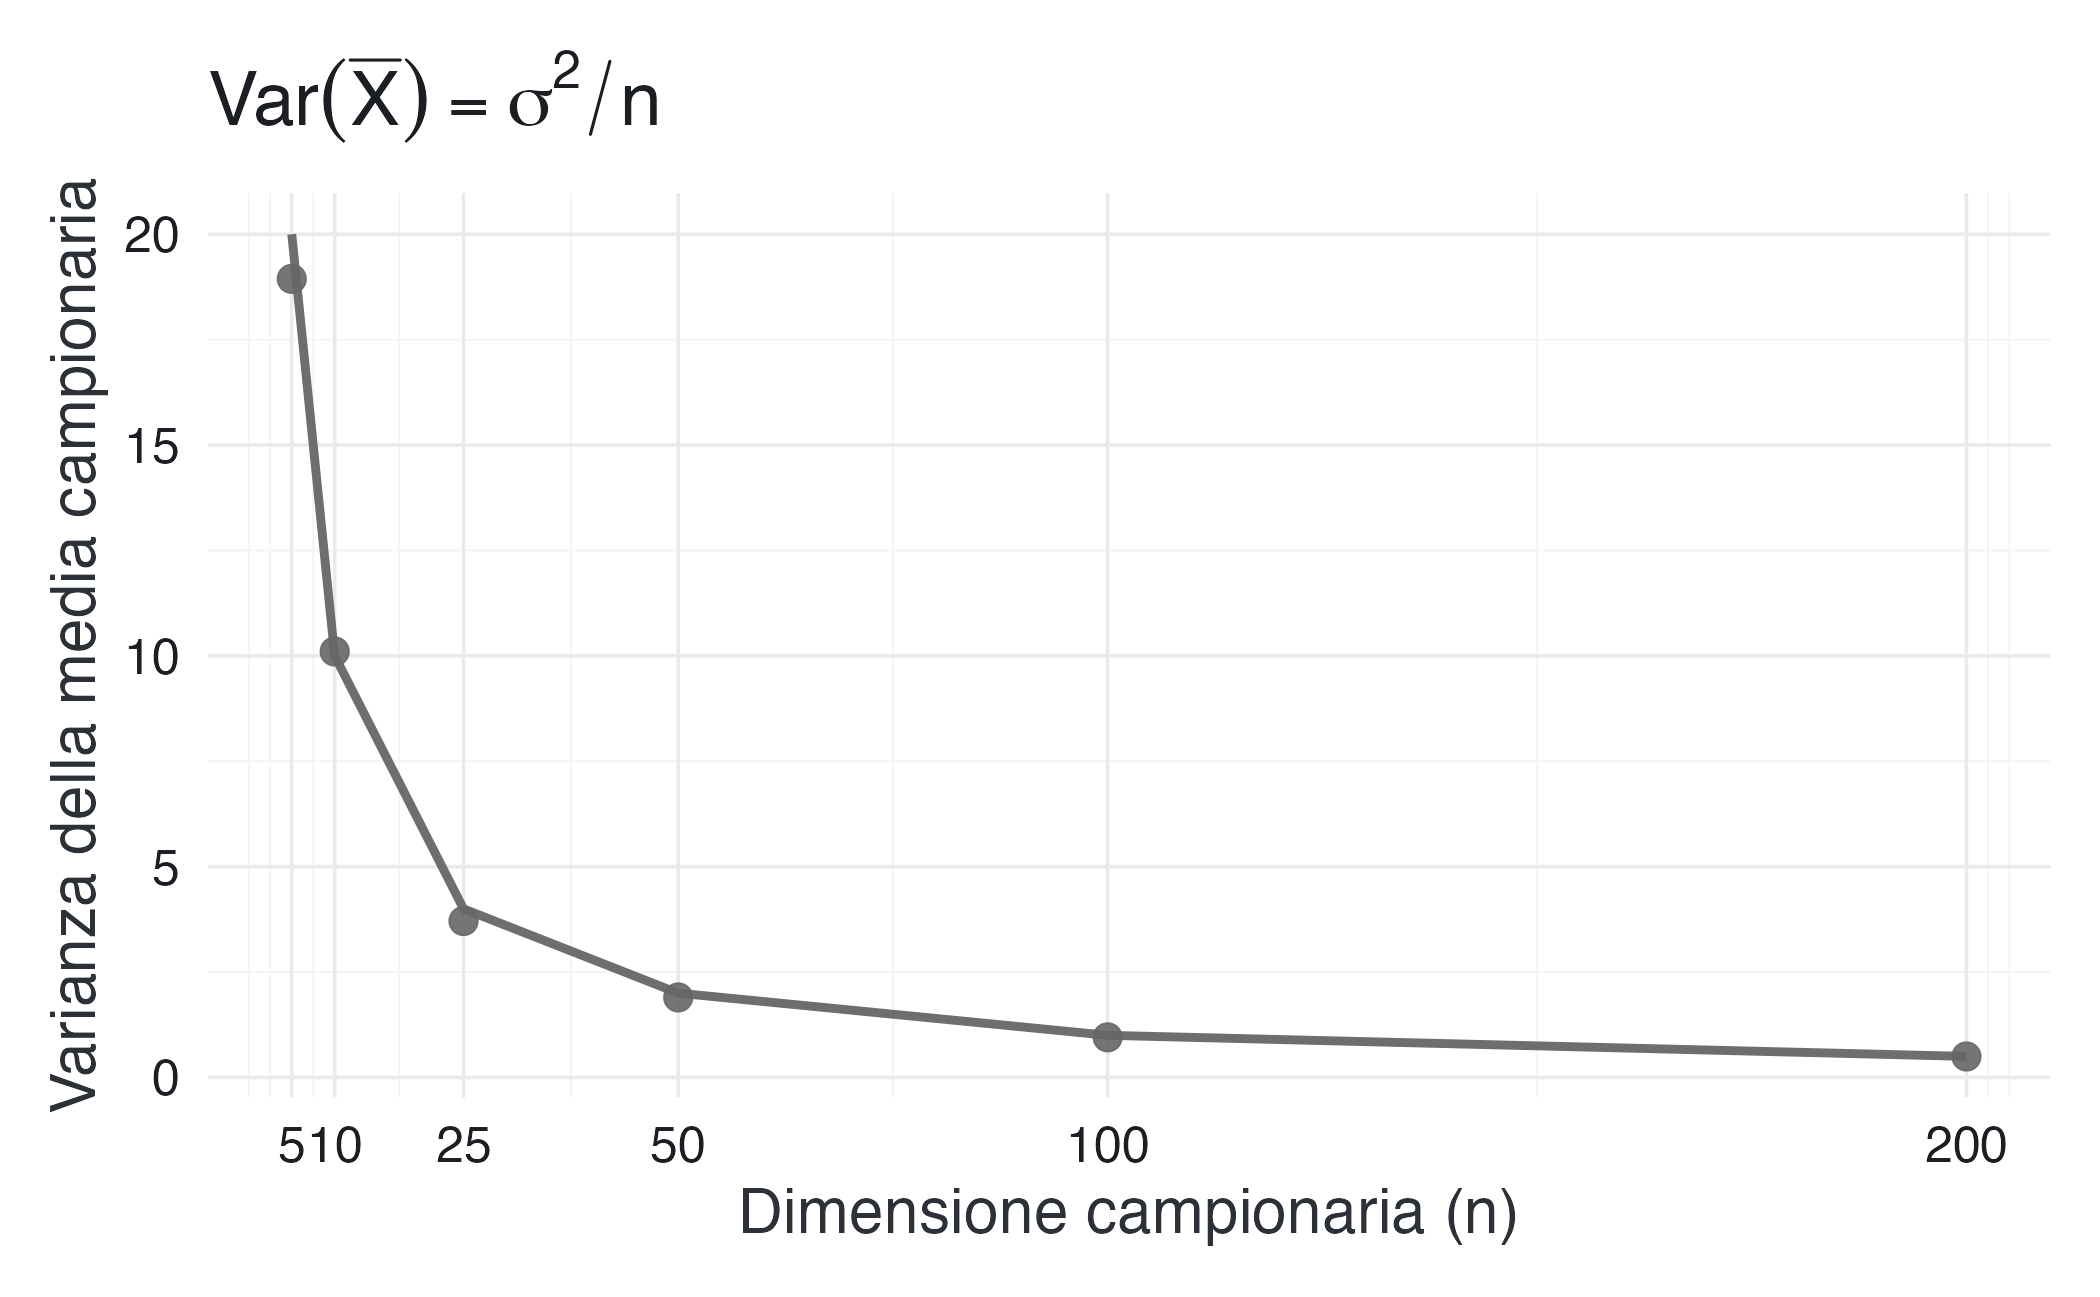
\includegraphics[width=0.85\linewidth,height=\textheight,keepaspectratio]{chapters/probability/08_expval_var_files/figure-pdf/fig-varianza-media-1.png}

}

\caption{\label{fig-varianza-media}La varianza della media campionaria
decresce con la dimensione del campione.}

\end{figure}%

\section{Deviazione standard e
standardizzazione}\label{sec-standard-deviation}

La varianza è espressa nel \textbf{quadrato} dell'unità di misura
originale. Per ottenere una misura di dispersione \textbf{nella stessa
scala} dei dati, si introduce la \emph{deviazione standard}.

\begin{definition}[Deviazione
standard]\protect\hypertarget{def-standard-deviation}{}\label{def-standard-deviation}

La \emph{deviazione standard} di una variabile casuale \(X\) è:

\[
\sigma_X = \text{SD}(X) = \sqrt{\text{Var}(X)}.
\]

\end{definition}

\subsection{Standardizzazione}\label{standardizzazione}

\begin{definition}[Variabile
standardizzata]\protect\hypertarget{def-standardization}{}\label{def-standardization}

Data \(X\) con \(\mathbb{E}[X] = \mu\) e \(\text{SD}(X) = \sigma\), la
\emph{variabile standardizzata} è:

\[
Z = \frac{X - \mu}{\sigma}.
\]

\end{definition}

La variabile standardizzata \(Z\) ha sempre \(\mathbb{E}[Z] = 0\) e
\(\text{Var}(Z) = 1\), indipendentemente dalla distribuzione originaria.

\begin{tcolorbox}[enhanced jigsaw, arc=.35mm, bottomrule=.15mm, bottomtitle=1mm, breakable, colback=white, colbacktitle=quarto-callout-note-color!10!white, colframe=quarto-callout-note-color-frame, coltitle=black, left=2mm, leftrule=.75mm, opacityback=0, opacitybacktitle=0.6, rightrule=.15mm, title=\textcolor{quarto-callout-note-color}{\faInfo}\hspace{0.5em}{Esempio: confronto tra scale psicometriche diverse}, titlerule=0mm, toprule=.15mm, toptitle=1mm]

\textbf{Paziente A}: BDI-II = 28 (\(\mu = 14\), \(\sigma = 10\)).
\textbf{Paziente B}: PHQ-9 = 18 (\(\mu = 10\), \(\sigma = 6\)).

\begin{Shaded}
\begin{Highlighting}[]
\NormalTok{z\_A }\OtherTok{\textless{}{-}}\NormalTok{ (}\DecValTok{28} \SpecialCharTok{{-}} \DecValTok{14}\NormalTok{) }\SpecialCharTok{/} \DecValTok{10}
\NormalTok{z\_B }\OtherTok{\textless{}{-}}\NormalTok{ (}\DecValTok{18} \SpecialCharTok{{-}} \DecValTok{10}\NormalTok{) }\SpecialCharTok{/} \DecValTok{6}

\FunctionTok{cat}\NormalTok{(}\StringTok{"Paziente A (BDI{-}II = 28): z ="}\NormalTok{, z\_A, }\StringTok{"}\SpecialCharTok{\textbackslash{}n}\StringTok{"}\NormalTok{)}
\CommentTok{\#\textgreater{} Paziente A (BDI{-}II = 28): z = 1.4}
\FunctionTok{cat}\NormalTok{(}\StringTok{"Paziente B (PHQ{-}9 = 18): z ="}\NormalTok{, }\FunctionTok{round}\NormalTok{(z\_B, }\DecValTok{2}\NormalTok{), }\StringTok{"}\SpecialCharTok{\textbackslash{}n\textbackslash{}n}\StringTok{"}\NormalTok{)}
\CommentTok{\#\textgreater{} Paziente B (PHQ{-}9 = 18): z = 1.33}

\FunctionTok{cat}\NormalTok{(}\StringTok{"Interpretazione: Il Paziente A mostra sintomi più gravi in termini relativi,}\SpecialCharTok{\textbackslash{}n}\StringTok{"}\NormalTok{)}
\CommentTok{\#\textgreater{} Interpretazione: Il Paziente A mostra sintomi più gravi in termini relativi,}
\FunctionTok{cat}\NormalTok{(}\StringTok{"essendo più lontano dalla media della sua distribuzione di riferimento.}\SpecialCharTok{\textbackslash{}n}\StringTok{"}\NormalTok{)}
\CommentTok{\#\textgreater{} essendo più lontano dalla media della sua distribuzione di riferimento.}
\end{Highlighting}
\end{Shaded}

\textbf{Conversione in T-score (media 50, SD 10):}

\begin{Shaded}
\begin{Highlighting}[]
\NormalTok{T\_A }\OtherTok{\textless{}{-}} \DecValTok{50} \SpecialCharTok{+} \DecValTok{10} \SpecialCharTok{*}\NormalTok{ z\_A}
\NormalTok{T\_B }\OtherTok{\textless{}{-}} \DecValTok{50} \SpecialCharTok{+} \DecValTok{10} \SpecialCharTok{*}\NormalTok{ z\_B}

\FunctionTok{cat}\NormalTok{(}\StringTok{"T{-}score Paziente A:"}\NormalTok{, T\_A, }\StringTok{"}\SpecialCharTok{\textbackslash{}n}\StringTok{"}\NormalTok{)}
\CommentTok{\#\textgreater{} T{-}score Paziente A: 64}
\FunctionTok{cat}\NormalTok{(}\StringTok{"T{-}score Paziente B:"}\NormalTok{, }\FunctionTok{round}\NormalTok{(T\_B, }\DecValTok{1}\NormalTok{), }\StringTok{"}\SpecialCharTok{\textbackslash{}n}\StringTok{"}\NormalTok{)}
\CommentTok{\#\textgreater{} T{-}score Paziente B: 63.3}
\end{Highlighting}
\end{Shaded}

I T-score permettono un confronto immediato su una scala comune.

\end{tcolorbox}

\subsection{Ponte applicativo: la standardizzazione nella pratica
clinica}\label{ponte-applicativo-la-standardizzazione-nella-pratica-clinica}

La trasformazione in punti z è uno strumento essenziale in psicometria
per:

\begin{enumerate}
\def\labelenumi{\arabic{enumi}.}
\tightlist
\item
  \textbf{Confrontare punteggi provenienti da scale diverse},
  neutralizzando le differenze di media e dispersione.
\item
  \textbf{Interpretare la posizione di un individuo} all'interno della
  distribuzione di riferimento.
\item
  \textbf{Identificare punteggi estremi}: convenzionalmente, \(|z| > 2\)
  è atipico, \(|z| > 3\) è molto raro.
\item
  \textbf{Costruire indicatori compositi} integrando misure con unità di
  misura differenti.
\end{enumerate}

\section{Il teorema di Chebyshev e i
momenti}\label{sec-chebyshev-moments}

\begin{tcolorbox}[enhanced jigsaw, arc=.35mm, bottomrule=.15mm, bottomtitle=1mm, breakable, colback=white, colbacktitle=quarto-callout-note-color!10!white, colframe=quarto-callout-note-color-frame, coltitle=black, left=2mm, leftrule=.75mm, opacityback=0, opacitybacktitle=0.6, rightrule=.15mm, title=\textcolor{quarto-callout-note-color}{\faInfo}\hspace{0.5em}{Approfondimento: il teorema di Chebyshev}, titlerule=0mm, toprule=.15mm, toptitle=1mm]

Una domanda che sorge naturalmente: \textbf{quanta probabilità si
concentra entro un certo numero di deviazioni standard dalla media?} Il
\emph{teorema di Chebyshev} fornisce una risposta universale,
applicabile a \textbf{qualsiasi distribuzione} con media e varianza
finite.

\begin{theorem}[]\protect\hypertarget{thm-chebyshev}{}\label{thm-chebyshev}

\textbf{Teorema di Chebyshev}

Sia \(X\) una variabile casuale con media \(\mu\) e deviazione standard
\(\sigma\). Per ogni \(k > 0\):

\[
P(|X - \mu| \geq k\sigma) \leq \frac{1}{k^2}.
\]

Equivalentemente:

\[
P(|X - \mu| < k\sigma) \geq 1 - \frac{1}{k^2}.
\]

\end{theorem}

{\def\LTcaptype{none} % do not increment counter
\begin{longtable}[]{@{}cc@{}}
\toprule\noalign{}
\(k\) & \(P(|X - \mu| < k\sigma) \geq\) \\
\midrule\noalign{}
\endhead
\bottomrule\noalign{}
\endlastfoot
2 & 75\% \\
3 & 88.9\% (\textasciitilde89\%) \\
4 & 93.75\% (\textasciitilde94\%) \\
\end{longtable}
}

Questi limiti sono \textbf{molto conservativi}. Per una distribuzione
normale, le probabilità effettive sono 68.3\%, 95.4\% e 99.7\% per
\(k = 1, 2, 3\).

\textbf{Applicazione clinica}

Immaginiamo che un test cognitivo abbia media 100 e deviazione standard
15, ma che nulla sia noto sulla forma della sua distribuzione. Grazie a
Chebyshev possiamo affermare che \textbf{almeno il 75\%} dei punteggi si
trova nell'intervallo \([70, 130]\), indipendentemente dalla
distribuzione.

\end{tcolorbox}

\begin{tcolorbox}[enhanced jigsaw, arc=.35mm, bottomrule=.15mm, bottomtitle=1mm, breakable, colback=white, colbacktitle=quarto-callout-note-color!10!white, colframe=quarto-callout-note-color-frame, coltitle=black, left=2mm, leftrule=.75mm, opacityback=0, opacitybacktitle=0.6, rightrule=.15mm, title=\textcolor{quarto-callout-note-color}{\faInfo}\hspace{0.5em}{Approfondimento: i momenti di una distribuzione}, titlerule=0mm, toprule=.15mm, toptitle=1mm]

\textbf{Momenti di una distribuzione}

Il valore atteso e la varianza possono essere visti come i primi due
\textbf{momenti} di una distribuzione.

\begin{definition}[]\protect\hypertarget{def-moments}{}\label{def-moments}

\textbf{Momenti}

Il \emph{momento di ordine \(r\)} di una variabile casuale \(X\) è:

\[
\mathbb{E}[X^r] =
\begin{cases}
\sum_i x_i^r \cdot p_X(x_i) & \text{(discreto)} \\
\int_{-\infty}^{+\infty} x^r \cdot f_X(x)\,dx & \text{(continuo)}
\end{cases}
\]

Il \emph{momento centrale di ordine \(r\)} è
\(\mathbb{E}[(X - \mu)^r]\), dove \(\mu = \mathbb{E}[X]\).

\end{definition}

\begin{itemize}
\tightlist
\item
  Il \textbf{momento di ordine 1} è il valore atteso (centro).
\item
  Il \textbf{momento centrale di ordine 2} è la varianza (dispersione).
\item
  Il \textbf{momento centrale di ordine 3} (normalizzato) è la
  \textbf{skewness} (asimmetria).
\item
  Il \textbf{momento centrale di ordine 4} (normalizzato) è la
  \textbf{kurtosis} (pesantezza delle code).
\end{itemize}

Questi concetti diventano rilevanti nella validazione di scale
psicometriche e nella scelta di modelli statistici appropriati.

\end{tcolorbox}

\section*{Riflessioni conclusive}\label{riflessioni-conclusive-7}

\markright{Riflessioni conclusive}

Il \textbf{valore atteso} e la \textbf{varianza} rappresentano i due
strumenti fondamentali per sintetizzare una distribuzione di
probabilità. Il primo identifica il centro della distribuzione; il
secondo misura la dispersione, quantificando l'\textbf{incertezza
residua}.

Per lo psicologo clinico, questi concetti sono strumenti operativi
quotidiani. Quando comunichiamo che ``il miglioramento atteso è di circa
8 punti'', ci riferiamo al valore atteso. Se aggiungiamo che ``la
maggior parte dei pazienti mostra un miglioramento compreso tra 4 e 12
punti'', stiamo descrivendo la varianza. Entrambi sono essenziali per
una comunicazione clinica completa.

La \textbf{linearità del valore atteso} permette di calcolare le medie
di somme e combinazioni lineari --- ecco perché il punteggio atteso di
una scala è la somma dei punteggi attesi dei suoi item. Il comportamento
della \textbf{varianza} sottolinea il ruolo cruciale dell'indipendenza:
soltanto in assenza di dipendenza la varianza di una somma coincide con
la somma delle varianze.

Il risultato \(\text{Var}(\bar{X}) = \sigma^2/n\) fornisce il
\textbf{fondamento matematico della precisione statistica}: maggiore è
il numero di osservazioni, minore è l'incertezza. Questo principio guida
la progettazione degli studi clinici.

Nel quadro bayesiano, questi concetti assumono una valenza pienamente
\textbf{inferenziale}. Il valore atteso della distribuzione \emph{a
posteriori} fungerà da \textbf{stima puntuale razionale}, mentre la sua
varianza misurerà l'incertezza residua dopo aver osservato i dati.

\section*{Punti chiave da ricordare}\label{punti-chiave-da-ricordare-7}
\addcontentsline{toc}{section}{Punti chiave da ricordare}

\markright{Punti chiave da ricordare}

\begin{tcolorbox}[enhanced jigsaw, arc=.35mm, bottomrule=.15mm, bottomtitle=1mm, breakable, colback=white, colbacktitle=quarto-callout-important-color!10!white, colframe=quarto-callout-important-color-frame, coltitle=black, left=2mm, leftrule=.75mm, opacityback=0, opacitybacktitle=0.6, rightrule=.15mm, title=\textcolor{quarto-callout-important-color}{\faExclamation}\hspace{0.5em}{Importante}, titlerule=0mm, toprule=.15mm, toptitle=1mm]

\begin{enumerate}
\def\labelenumi{\arabic{enumi}.}
\tightlist
\item
  \textbf{Valore atteso come centro di gravità probabilistico}

  \begin{itemize}
  \tightlist
  \item
    Media ponderata dei valori possibili con pesi probabilistici.
  \item
    Non deve necessariamente coincidere con un valore osservabile.
  \item
    Legge dei grandi numeri: la media campionaria converge al valore
    atteso.
  \end{itemize}
\item
  \textbf{Linearità del valore atteso}

  \begin{itemize}
  \tightlist
  \item
    \(\mathbb{E}[X + Y] = \mathbb{E}[X] + \mathbb{E}[Y]\)
    \textbf{sempre} (anche con dipendenza).
  \item
    \(\mathbb{E}[aX + b] = a\mathbb{E}[X] + b\).
  \item
    Applicazione: il punteggio atteso di una scala è la somma dei valori
    attesi degli item.
  \end{itemize}
\item
  \textbf{Varianza come misura di dispersione e incertezza}

  \begin{itemize}
  \tightlist
  \item
    \(\text{Var}(X) = \mathbb{E}[(X - \mu)^2]\) quantifica la
    dispersione.
  \item
    Interpretazione epistemica: perdita attesa usando il valore atteso
    come previsione.
  \item
    Formula computazionale:
    \(\text{Var}(X) = \mathbb{E}[X^2] - (\mathbb{E}[X])^2\).
  \end{itemize}
\item
  \textbf{Proprietà della varianza}

  \begin{itemize}
  \tightlist
  \item
    \(\text{Var}(aX + b) = a^2 \text{Var}(X)\).
  \item
    \(\text{Var}(X + Y) = \text{Var}(X) + \text{Var}(Y)\) \textbf{solo
    se} \(X \perp Y\).
  \item
    \(\text{Var}(\bar{X}) = \sigma^2/n\) (fondamento della precisione
    statistica).
  \end{itemize}
\item
  \textbf{Deviazione standard e standardizzazione}

  \begin{itemize}
  \tightlist
  \item
    \(\sigma = \sqrt{\text{Var}(X)}\) riporta la dispersione nelle unità
    originali.
  \item
    \(Z = (X - \mu)/\sigma\) ha media 0 e varianza 1.
  \item
    Permette confronti tra scale diverse.
  \end{itemize}
\end{enumerate}

\textbf{Formule da ricordare:}

\[
\mathbb{E}[X] = \sum_x x \cdot p_X(x) \quad \text{o} \quad \int x \cdot f_X(x)\,dx
\]

\[
\text{Var}(X) = \mathbb{E}[X^2] - (\mathbb{E}[X])^2
\]

\[
\text{Var}(\bar{X}_n) = \frac{\sigma^2}{n}
\]

\textbf{Per il prossimo capitolo:}

Nel Capitolo~\ref{sec-prob-cov-cor} studieremo come quantificare la
\textbf{dipendenza stocastica} tra due variabili attraverso covarianza e
correlazione, concetti essenziali per comprendere quando l'additività
della varianza fallisce e per costruire modelli che catturano le
relazioni tra variabili psicologiche.

\end{tcolorbox}

\begin{tcolorbox}[enhanced jigsaw, arc=.35mm, bottomrule=.15mm, bottomtitle=1mm, breakable, colback=white, colbacktitle=quarto-callout-note-color!10!white, colframe=quarto-callout-note-color-frame, coltitle=black, left=2mm, leftrule=.75mm, opacityback=0, opacitybacktitle=0.6, rightrule=.15mm, title=\textcolor{quarto-callout-note-color}{\faInfo}\hspace{0.5em}{Informazioni sull'ambiente di sviluppo}, titlerule=0mm, toprule=.15mm, toptitle=1mm]

\begin{Shaded}
\begin{Highlighting}[]
\FunctionTok{sessionInfo}\NormalTok{()}
\CommentTok{\#\textgreater{} R version 4.6.1 (2026{-}06{-}24)}
\CommentTok{\#\textgreater{} Platform: aarch64{-}apple{-}darwin23}
\CommentTok{\#\textgreater{} Running under: macOS Tahoe 26.5.2}
\CommentTok{\#\textgreater{} }
\CommentTok{\#\textgreater{} Matrix products: default}
\CommentTok{\#\textgreater{} BLAS:   /Library/Frameworks/R.framework/Versions/4.6/Resources/lib/libRblas.0.dylib }
\CommentTok{\#\textgreater{} LAPACK: /Library/Frameworks/R.framework/Versions/4.6/Resources/lib/libRlapack.dylib;  LAPACK version 3.12.1}
\CommentTok{\#\textgreater{} }
\CommentTok{\#\textgreater{} locale:}
\CommentTok{\#\textgreater{} [1] C.UTF{-}8/UTF{-}8/C.UTF{-}8/C/C.UTF{-}8/C.UTF{-}8}
\CommentTok{\#\textgreater{} }
\CommentTok{\#\textgreater{} time zone: Europe/Rome}
\CommentTok{\#\textgreater{} tzcode source: internal}
\CommentTok{\#\textgreater{} }
\CommentTok{\#\textgreater{} attached base packages:}
\CommentTok{\#\textgreater{} [1] stats     graphics  grDevices utils     datasets  methods   base     }
\CommentTok{\#\textgreater{} }
\CommentTok{\#\textgreater{} other attached packages:}
\CommentTok{\#\textgreater{}  [1] MASS\_7.3{-}65           ragg\_1.5.2            tinytable\_0.17.0     }
\CommentTok{\#\textgreater{}  [4] withr\_3.0.3           systemfonts\_1.3.2     patchwork\_1.3.2      }
\CommentTok{\#\textgreater{}  [7] ggdist\_3.3.3          tidybayes\_3.0.7       bayesplot\_1.15.0     }
\CommentTok{\#\textgreater{} [10] ggplot2\_4.0.3         reliabilitydiag\_0.2.1 priorsense\_1.2.0     }
\CommentTok{\#\textgreater{} [13] posterior\_1.7.0       loo\_2.10.0            rstan\_2.32.7         }
\CommentTok{\#\textgreater{} [16] StanHeaders\_2.32.10   brms\_2.23.0           Rcpp\_1.1.2           }
\CommentTok{\#\textgreater{} [19] sessioninfo\_1.2.4     conflicted\_1.2.0      janitor\_2.2.1        }
\CommentTok{\#\textgreater{} [22] matrixStats\_1.5.0     modelr\_0.1.11         tibble\_3.3.1         }
\CommentTok{\#\textgreater{} [25] dplyr\_1.2.1           tidyr\_1.3.2           rio\_1.3.0            }
\CommentTok{\#\textgreater{} [28] here\_1.0.2           }
\CommentTok{\#\textgreater{} }
\CommentTok{\#\textgreater{} loaded via a namespace (and not attached):}
\CommentTok{\#\textgreater{}  [1] svUnit\_1.0.8          tidyselect\_1.2.1      farver\_2.1.2         }
\CommentTok{\#\textgreater{}  [4] S7\_0.2.2              fastmap\_1.2.0         tensorA\_0.36.2.1     }
\CommentTok{\#\textgreater{}  [7] digest\_0.6.39         timechange\_0.4.0      estimability\_2.0.0   }
\CommentTok{\#\textgreater{} [10] lifecycle\_1.0.5       magrittr\_2.0.5        compiler\_4.6.1       }
\CommentTok{\#\textgreater{} [13] rlang\_1.3.0           tools\_4.6.1           yaml\_2.3.12          }
\CommentTok{\#\textgreater{} [16] knitr\_1.51            labeling\_0.4.3        bridgesampling\_1.2{-}1 }
\CommentTok{\#\textgreater{} [19] pkgbuild\_1.4.8        curl\_7.1.0            RColorBrewer\_1.1{-}3   }
\CommentTok{\#\textgreater{} [22] abind\_1.4{-}8           purrr\_1.2.2           grid\_4.6.1           }
\CommentTok{\#\textgreater{} [25] stats4\_4.6.1          xtable\_1.8{-}8          inline\_0.3.21        }
\CommentTok{\#\textgreater{} [28] emmeans\_2.0.3         scales\_1.4.0          cli\_3.6.6            }
\CommentTok{\#\textgreater{} [31] mvtnorm\_1.4{-}1         rmarkdown\_2.31        generics\_0.1.4       }
\CommentTok{\#\textgreater{} [34] otel\_0.2.0            RcppParallel\_5.1.11{-}2 cachem\_1.1.0         }
\CommentTok{\#\textgreater{} [37] stringr\_1.6.0         parallel\_4.6.1        vctrs\_0.7.3          }
\CommentTok{\#\textgreater{} [40] V8\_8.2.0              Matrix\_1.7{-}5          jsonlite\_2.0.0       }
\CommentTok{\#\textgreater{} [43] arrayhelpers\_1.1{-}1    glue\_1.8.1            codetools\_0.2{-}20     }
\CommentTok{\#\textgreater{} [46] distributional\_0.8.1  lubridate\_1.9.5       stringi\_1.8.7        }
\CommentTok{\#\textgreater{} [49] gtable\_0.3.6          QuickJSR\_1.10.0       pillar\_1.11.1        }
\CommentTok{\#\textgreater{} [52] htmltools\_0.5.9       Brobdingnag\_1.2{-}9     R6\_2.6.1             }
\CommentTok{\#\textgreater{} [55] textshaping\_1.0.5     rprojroot\_2.1.1       evaluate\_1.0.5       }
\CommentTok{\#\textgreater{} [58] lattice\_0.22{-}9        backports\_1.5.1       memoise\_2.0.1        }
\CommentTok{\#\textgreater{} [61] broom\_1.0.13          snakecase\_0.11.1      rstantools\_2.6.0     }
\CommentTok{\#\textgreater{} [64] coda\_0.19{-}4.1         gridExtra\_2.3.1       nlme\_3.1{-}169         }
\CommentTok{\#\textgreater{} [67] checkmate\_2.3.4       xfun\_0.60             pkgconfig\_2.0.3}
\end{Highlighting}
\end{Shaded}

\end{tcolorbox}

\chapter{Covarianza e correlazione}\label{sec-prob-cov-cor}

\section*{Introduzione}\label{introduzione-8}

\markright{Introduzione}

Un ricercatore sta analizzando i dati di uno studio sulla relazione tra
ansia e prestazione cognitiva negli studenti universitari. I risultati
preliminari mostrano che, in media, livelli più alti di ansia si
associano a punteggi più bassi nei test di memoria di lavoro. Ma quanto
è robusta questa associazione? È clinicamente o teoricamente rilevante?
E come possiamo comunicare questo risultato in modo che sia
confrontabile con altri studi?

Queste domande richiedono strumenti che vadano oltre la descrizione di
tendenze generali. La \textbf{covarianza} quantifica la tendenza di due
variabili a variare insieme in modo sistematico, mentre la
\textbf{correlazione} standardizza tale misura su una scala universale,
permettendo confronti trasversali.

Dal punto di vista bayesiano, covarianza e correlazione possono essere
interpretate come \textbf{riassunti quantitativi della struttura delle
nostre credenze}, codificata nella distribuzione congiunta. Quando
affermiamo che due variabili sono correlate negativamente con
\(\rho = -0.40\), stiamo esprimendo una proprietà specifica di come
crediamo che queste variabili si comportino congiuntamente.

In questo capitolo:

\begin{enumerate}
\def\labelenumi{\arabic{enumi}.}
\tightlist
\item
  \textbf{Estenderemo} il framework delle distribuzioni congiunte al
  caso continuo.
\item
  \textbf{Definiremo} la covarianza come misura della co-variazione
  lineare.
\item
  \textbf{Introdurremo} la correlazione come versione standardizzata.
\item
  \textbf{Discuteremo} le proprietà matematiche e il loro significato
  pratico.
\item
  \textbf{Chiariremo} la distinzione tra incorrelazione e indipendenza.
\item
  \textbf{Accenneremo} al ruolo della covarianza nell'inferenza
  bayesiana.
\end{enumerate}

\begin{tcolorbox}[enhanced jigsaw, arc=.35mm, bottomrule=.15mm, bottomtitle=1mm, breakable, colback=white, colbacktitle=quarto-callout-tip-color!10!white, colframe=quarto-callout-tip-color-frame, coltitle=black, left=2mm, leftrule=.75mm, opacityback=0, opacitybacktitle=0.6, rightrule=.15mm, title=\textcolor{quarto-callout-tip-color}{\faLightbulb}\hspace{0.5em}{Prerequisiti}, titlerule=0mm, toprule=.15mm, toptitle=1mm]

Per seguire questo capitolo è necessario aver letto:

\begin{itemize}
\tightlist
\item
  Capitolo~\ref{sec-prob-random-var} --- per il concetto di variabili
  casuali multiple.
\item
  Capitolo~\ref{sec-prob-random-var-properties} ---
  \textbf{fondamentale} per valore atteso e varianza.
\end{itemize}

Conoscenze matematiche richieste:

\begin{itemize}
\tightlist
\item
  Appendice~\ref{sec-apx-sums} - per calcoli con distribuzioni discrete
  congiunte.
\item
  Appendice~\ref{sec-apx-calculus} - per densità congiunte continue.
\end{itemize}

Competenze pratiche:

\begin{itemize}
\tightlist
\item
  Familiarità con R e visualizzazione di distribuzioni bivariate.
\end{itemize}

\end{tcolorbox}

\begin{tcolorbox}[enhanced jigsaw, arc=.35mm, bottomrule=.15mm, bottomtitle=1mm, breakable, colback=white, colbacktitle=quarto-callout-caution-color!10!white, colframe=quarto-callout-caution-color-frame, coltitle=black, left=2mm, leftrule=.75mm, opacityback=0, opacitybacktitle=0.6, rightrule=.15mm, title=\textcolor{quarto-callout-caution-color}{\faFire}\hspace{0.5em}{Preparazione del Notebook}, titlerule=0mm, toprule=.15mm, toptitle=1mm]

\begin{Shaded}
\begin{Highlighting}[]
\NormalTok{here}\SpecialCharTok{::}\FunctionTok{here}\NormalTok{(}\StringTok{"code"}\NormalTok{, }\StringTok{"\_common.R"}\NormalTok{) }\SpecialCharTok{|\textgreater{}}
  \FunctionTok{source}\NormalTok{()}

\FunctionTok{library}\NormalTok{(MASS)}
\FunctionTok{library}\NormalTok{(viridis)}
\FunctionTok{library}\NormalTok{(ggExtra)}

\CommentTok{\# Riapplica il tema per sicurezza}
\FunctionTok{apply\_visual\_theme}\NormalTok{()}
\end{Highlighting}
\end{Shaded}

\end{tcolorbox}

\section{Dalle tabelle discrete alle densità
continue}\label{sec-from-discrete-to-continuous}

Nel capitolo sugli assiomi (Capitolo~\ref{sec-prob-axioms-coherence})
abbiamo utilizzato tabelle congiunte per rappresentare le nostre
credenze su coppie di variabili binarie. Gli stessi principi si
estendono a situazioni più complesse: tabelle con più categorie e
densità congiunte per variabili continue.

\subsection{Tabelle con più
categorie}\label{tabelle-con-piuxf9-categorie}

Consideriamo la relazione tra ansia e prestazione cognitiva. Numerosi
studi suggeriscono una relazione negativa tra questi fattori
(\citeproc{ref-eysenck2007anxiety}{Eysenck et al., 2007}). Supponiamo di
codificare l'ansia in tre livelli (bassa, media, alta) e la prestazione
in tre livelli (insufficiente, sufficiente, buona).

Una possibile distribuzione congiunta che rappresenta le nostre
credenze, informate dalla letteratura:

{\def\LTcaptype{none} % do not increment counter
\begin{longtable}[]{@{}lllll@{}}
\toprule\noalign{}
& Ansia Bassa & Ansia Media & Ansia Alta & Marginale \\
\midrule\noalign{}
\endhead
\bottomrule\noalign{}
\endlastfoot
\textbf{Insufficiente} & 0.05 & 0.10 & 0.15 & 0.30 \\
\textbf{Sufficiente} & 0.15 & 0.20 & 0.10 & 0.45 \\
\textbf{Buona} & 0.10 & 0.10 & 0.05 & 0.25 \\
\textbf{Marginale} & 0.30 & 0.40 & 0.30 & 1.00 \\
\end{longtable}
}

Ogni cella rappresenta il nostro grado di credenza in una specifica
configurazione. I principi di costruzione sono gli stessi visti per le
tabelle 2×2: le marginali si ottengono sommando, le condizionate
dividendo per la marginale appropriata.

\subsection{Il caso continuo: densità
congiunte}\label{il-caso-continuo-densituxe0-congiunte}

Quando le variabili assumono valori continui, la distribuzione congiunta
viene descritta mediante una \textbf{densità congiunta} \(f(x,y)\).

\begin{definition}[]\protect\hypertarget{def-joint-density}{}\label{def-joint-density}

Una \emph{densità congiunta} \(f(x,y)\) assegna a ogni configurazione
\((x,y)\) un valore che rappresenta la concentrazione della credenza in
quella regione. Per essere coerente, deve soddisfare:

\begin{enumerate}
\def\labelenumi{\arabic{enumi}.}
\tightlist
\item
  \textbf{Non negatività}: \(f(x,y) \geq 0\) per ogni \((x,y)\);
\item
  \textbf{Normalizzazione}:
  \(\int_{-\infty}^{+\infty} \int_{-\infty}^{+\infty} f(x,y)\,dx\,dy = 1\).
\end{enumerate}

\end{definition}

Le densità marginali si ottengono integrando rispetto a una delle
variabili:

\[
f_X(x) = \int_{-\infty}^{+\infty} f(x,y)\,dy,
\qquad
f_Y(y) = \int_{-\infty}^{+\infty} f(x,y)\,dx.
\]

Le densità condizionate si ottengono dividendo la densità congiunta per
la marginale appropriata:

\[
f_{X \mid Y}(x \mid y) = \frac{f(x,y)}{f_Y(y)}.
\]

\subsection{Regole di somma e prodotto per le densità
congiunte}\label{regole-di-somma-e-prodotto-per-le-densituxe0-congiunte}

Le regole si applicano senza modifiche concettuali, sostituendo le somme
con gli integrali.

\begin{itemize}
\tightlist
\item
  \textbf{Regola di somma (marginalizzazione)}:
  \(f_Y(y) = \int_{-\infty}^{+\infty} f_{X,Y}(x,y)\,dx\).
\item
  \textbf{Regola di prodotto}:
  \(f_{X,Y}(x,y) = f_{Y \mid X}(y \mid x) f_X(x) = f_{X \mid Y}(x \mid y) f_Y(y)\).
\end{itemize}

Queste relazioni mostrano che conoscere la distribuzione congiunta
equivale a conoscere tutte le marginali e condizionate.

\subsection{Visualizzazione di una distribuzione congiunta
continua}\label{visualizzazione-di-una-distribuzione-congiunta-continua}

Modelliamo la relazione ansia-prestazione come una distribuzione
continua.

\begin{center}
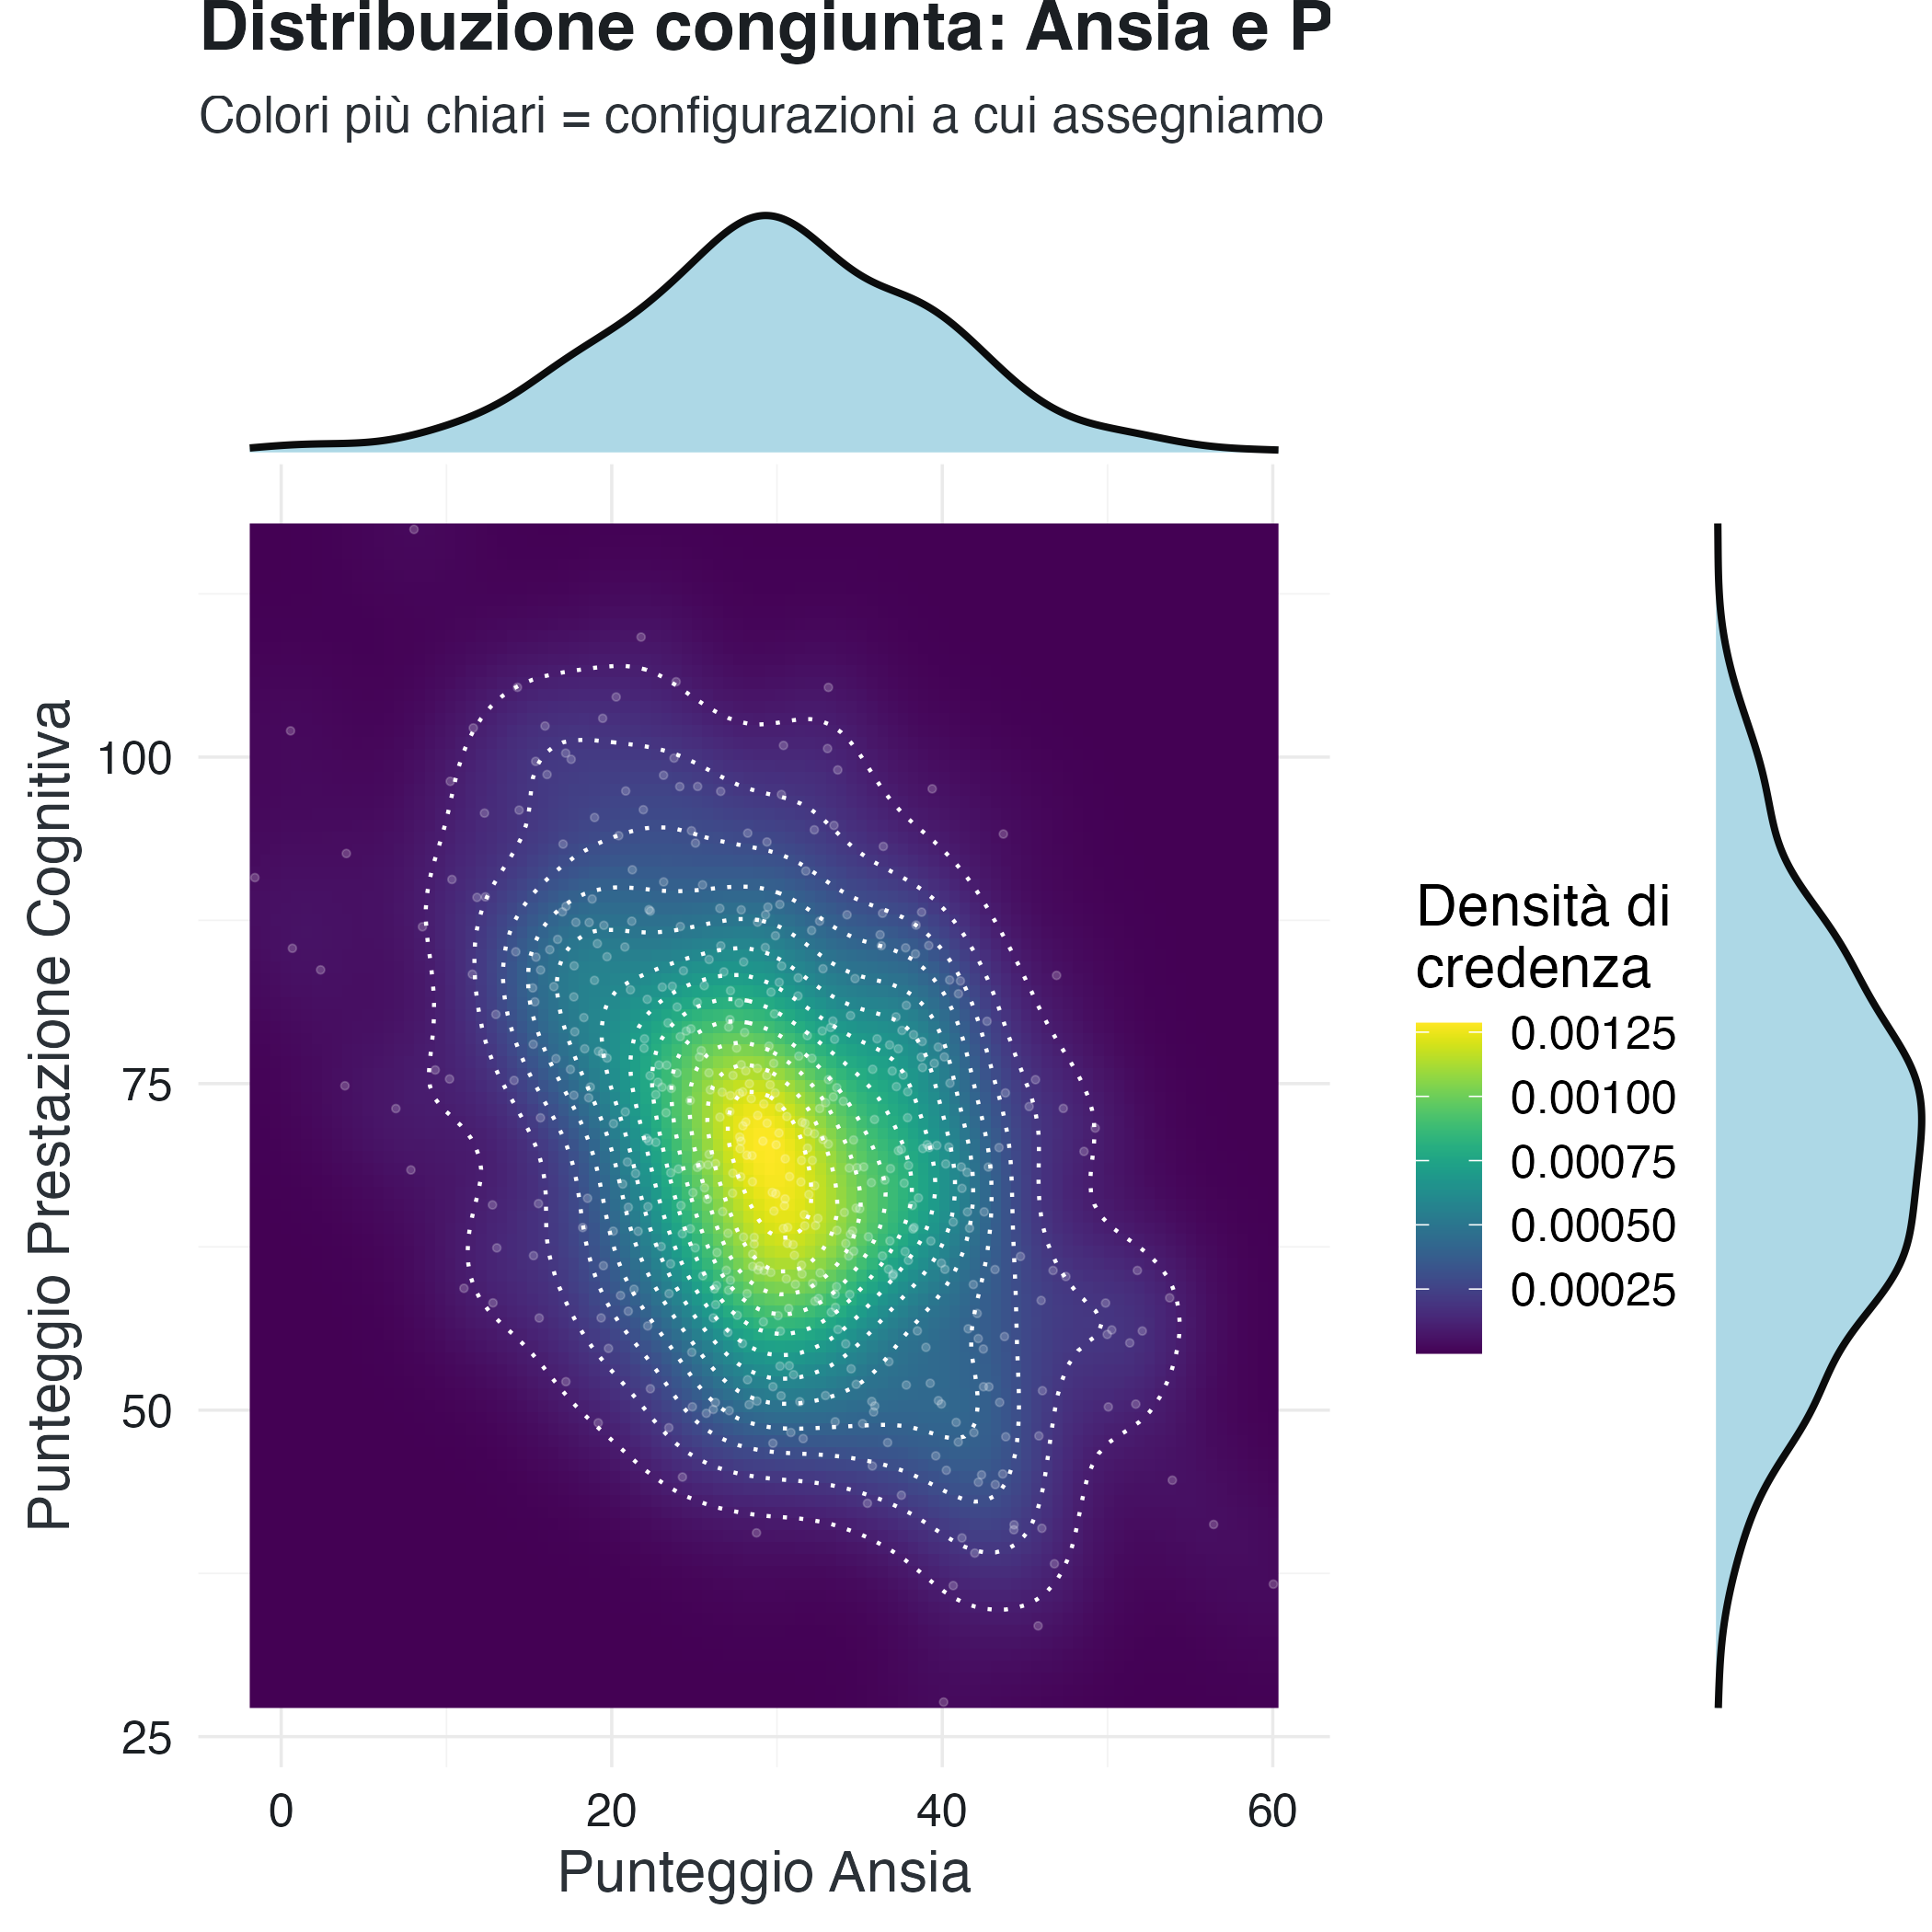
\includegraphics[width=0.85\linewidth,height=\textheight,keepaspectratio]{chapters/probability/09_cov_cor_files/figure-pdf/unnamed-chunk-2-1.png}
\end{center}

La regione più chiara (bassa ansia, buona prestazione) rappresenta le
configurazioni a cui attribuiamo la massima credibilità. L'orientamento
ellittico, inclinato verso il basso, riflette la correlazione negativa.

\begin{tcolorbox}[enhanced jigsaw, arc=.35mm, bottomrule=.15mm, bottomtitle=1mm, breakable, colback=white, colbacktitle=quarto-callout-important-color!10!white, colframe=quarto-callout-important-color-frame, coltitle=black, left=2mm, leftrule=.75mm, opacityback=0, opacitybacktitle=0.6, rightrule=.15mm, title=\textcolor{quarto-callout-important-color}{\faExclamation}\hspace{0.5em}{Dalla distribuzione congiunta ai riassunti numerici}, titlerule=0mm, toprule=.15mm, toptitle=1mm]

La distribuzione congiunta contiene tutta l'informazione sulle relazioni
tra le variabili. Tuttavia, comunicare un'intera distribuzione può
risultare complesso.

La covarianza e la correlazione sono riassunti numerici che:

\begin{itemize}
\tightlist
\item
  catturano l'aspetto \emph{lineare} della relazione;
\item
  condensano l'informazione in un singolo numero;
\item
  comportano una perdita di informazione: dipendenze non lineari possono
  esistere anche in presenza di correlazione nulla.
\end{itemize}

Questi indici sono strumenti utili ma parziali: la distribuzione
congiunta resta la fonte primaria dell'informazione.

\end{tcolorbox}

\section{Covarianza: misura della co-variazione
lineare}\label{sec-covariance}

\subsection{La domanda fondamentale}\label{la-domanda-fondamentale}

Quando diciamo che due variabili ``co-variano'', intendiamo che tendono
a muoversi insieme in modo sistematico:

\begin{itemize}
\tightlist
\item
  Quando l'ansia è sopra la sua media, la prestazione tende a essere
  sotto la sua media?
\item
  Quando il supporto sociale è elevato, il benessere tende a essere
  elevato?
\end{itemize}

La covarianza formalizza questa intuizione.

\begin{definition}[Covarianza]\protect\hypertarget{def-covariance}{}\label{def-covariance}

La \emph{covarianza} tra due variabili casuali \(X\) e \(Y\) è:

\[
\text{Cov}(X, Y) = \mathbb{E}\left[(X - \mathbb{E}[X])(Y - \mathbb{E}[Y])\right].
\]

Per variabili discrete con distribuzione congiunta \(p(x,y)\):

\[
\text{Cov}(X, Y) = \sum_{x}\sum_{y}(x - \mu_X)(y - \mu_Y)\,p(x, y).
\]

\end{definition}

L'interpretazione emerge dalla struttura del prodotto
\((X - \mu_X)(Y - \mu_Y)\):

\begin{itemize}
\tightlist
\item
  quando \textbf{entrambe} sono sopra le medie, il prodotto è
  \textbf{positivo};
\item
  quando \textbf{entrambe} sono sotto, il prodotto è \textbf{positivo};
\item
  quando una è sopra e l'altra sotto, il prodotto è \textbf{negativo}.
\end{itemize}

La covarianza è la media di questi prodotti:

\begin{itemize}
\tightlist
\item
  \textbf{positiva}: le variabili tendono a muoversi nella stessa
  direzione;
\item
  \textbf{negativa}: tendono a muoversi in direzioni opposte;
\item
  \textbf{nulla}: assenza di tendenza \emph{lineare} sistematica.
\end{itemize}

\subsection{Formula computazionale}\label{formula-computazionale}

\[
\text{Cov}(X, Y) = \mathbb{E}[XY] - \mathbb{E}[X]\mathbb{E}[Y].
\]

Questa espressione confronta il valore atteso del prodotto \(XY\) sotto
la distribuzione congiunta effettiva con il valore che si otterrebbe se
le variabili fossero \textbf{indipendenti}. La differenza misura quanto
la distribuzione congiunta si discosti dall'indipendenza.

\begin{tcolorbox}[enhanced jigsaw, arc=.35mm, bottomrule=.15mm, bottomtitle=1mm, breakable, colback=white, colbacktitle=quarto-callout-note-color!10!white, colframe=quarto-callout-note-color-frame, coltitle=black, left=2mm, leftrule=.75mm, opacityback=0, opacitybacktitle=0.6, rightrule=.15mm, title=\textcolor{quarto-callout-note-color}{\faInfo}\hspace{0.5em}{Esempio: calcolo dalla tabella congiunta}, titlerule=0mm, toprule=.15mm, toptitle=1mm]

Applichiamo i concetti alla tabella ansia-prestazione con codifica
numerica: prestazione \(X \in \{0,1,2\}\) e ansia \(Y \in \{0,1,2\}\).

\begin{Shaded}
\begin{Highlighting}[]
\NormalTok{tab\_joint }\OtherTok{\textless{}{-}} \FunctionTok{matrix}\NormalTok{(}
  \FunctionTok{c}\NormalTok{(}\FloatTok{0.05}\NormalTok{, }\FloatTok{0.10}\NormalTok{, }\FloatTok{0.15}\NormalTok{,}
    \FloatTok{0.15}\NormalTok{, }\FloatTok{0.20}\NormalTok{, }\FloatTok{0.10}\NormalTok{,}
    \FloatTok{0.10}\NormalTok{, }\FloatTok{0.10}\NormalTok{, }\FloatTok{0.05}\NormalTok{),}
  \AttributeTok{nrow =} \DecValTok{3}\NormalTok{, }\AttributeTok{byrow =} \ConstantTok{TRUE}\NormalTok{,}
  \AttributeTok{dimnames =} \FunctionTok{list}\NormalTok{(}
    \AttributeTok{Prestazione =} \FunctionTok{c}\NormalTok{(}\StringTok{"Insufficiente (0)"}\NormalTok{, }\StringTok{"Sufficiente (1)"}\NormalTok{, }\StringTok{"Buona (2)"}\NormalTok{),}
    \AttributeTok{Ansia =} \FunctionTok{c}\NormalTok{(}\StringTok{"Bassa (0)"}\NormalTok{, }\StringTok{"Media (1)"}\NormalTok{, }\StringTok{"Alta (2)"}\NormalTok{)}
\NormalTok{  )}
\NormalTok{)}

\NormalTok{val\_prest }\OtherTok{\textless{}{-}} \DecValTok{0}\SpecialCharTok{:}\DecValTok{2}
\NormalTok{val\_ansia }\OtherTok{\textless{}{-}} \DecValTok{0}\SpecialCharTok{:}\DecValTok{2}
\NormalTok{marg\_prest }\OtherTok{\textless{}{-}} \FunctionTok{rowSums}\NormalTok{(tab\_joint)}
\NormalTok{marg\_ansia }\OtherTok{\textless{}{-}} \FunctionTok{colSums}\NormalTok{(tab\_joint)}

\NormalTok{E\_X }\OtherTok{\textless{}{-}} \FunctionTok{sum}\NormalTok{(val\_prest }\SpecialCharTok{*}\NormalTok{ marg\_prest)}
\NormalTok{E\_Y }\OtherTok{\textless{}{-}} \FunctionTok{sum}\NormalTok{(val\_ansia }\SpecialCharTok{*}\NormalTok{ marg\_ansia)}

\NormalTok{E\_XY }\OtherTok{\textless{}{-}} \DecValTok{0}
\ControlFlowTok{for}\NormalTok{ (i }\ControlFlowTok{in} \DecValTok{1}\SpecialCharTok{:}\DecValTok{3}\NormalTok{) \{}
  \ControlFlowTok{for}\NormalTok{ (j }\ControlFlowTok{in} \DecValTok{1}\SpecialCharTok{:}\DecValTok{3}\NormalTok{) \{}
\NormalTok{    E\_XY }\OtherTok{\textless{}{-}}\NormalTok{ E\_XY }\SpecialCharTok{+}\NormalTok{ val\_prest[i] }\SpecialCharTok{*}\NormalTok{ val\_ansia[j] }\SpecialCharTok{*}\NormalTok{ tab\_joint[i, j]}
\NormalTok{  \}}
\NormalTok{\}}

\NormalTok{Cov\_XY }\OtherTok{\textless{}{-}}\NormalTok{ E\_XY }\SpecialCharTok{{-}}\NormalTok{ E\_X }\SpecialCharTok{*}\NormalTok{ E\_Y}

\FunctionTok{cat}\NormalTok{(}\StringTok{"Cov(X,Y) ="}\NormalTok{, }\FunctionTok{round}\NormalTok{(Cov\_XY, }\DecValTok{3}\NormalTok{), }\StringTok{"}\SpecialCharTok{\textbackslash{}n}\StringTok{"}\NormalTok{)}
\CommentTok{\#\textgreater{} Cov(X,Y) = {-}0.15}
\end{Highlighting}
\end{Shaded}

La covarianza negativa riflette la struttura delle nostre credenze: alta
ansia si accompagna a bassa prestazione.

\end{tcolorbox}

\section{Correlazione: covarianza standardizzata}\label{sec-correlation}

\subsection{Il problema delle unità di
misura}\label{il-problema-delle-unituxe0-di-misura}

La covarianza dipende dalle unità di misura. Se misurassimo l'ansia su
una scala da 0 a 100 anziché da 0 a 2, la covarianza cambierebbe, anche
se la relazione rimanesse invariata.

La \textbf{correlazione} risolve questo problema standardizzando la
covarianza.

\begin{definition}[Coefficiente di
correlazione]\protect\hypertarget{def-correlation}{}\label{def-correlation}

Il \emph{coefficiente di correlazione} (o correlazione di Pearson) tra
\(X\) e \(Y\) è:

\[
\rho(X,Y) = \frac{\text{Cov}(X,Y)}{\sqrt{\mathbb{V}(X)\,\mathbb{V}(Y)}} = \frac{\text{Cov}(X,Y)}{\sigma_X \sigma_Y}.
\]

\end{definition}

\subsection{Proprietà fondamentali}\label{proprietuxe0-fondamentali}

\begin{enumerate}
\def\labelenumi{\arabic{enumi}.}
\item
  \textbf{Limitatezza}: \(-1 \leq \rho(X,Y) \leq 1\).
\item
  \textbf{Invarianza rispetto a trasformazioni lineari}: se \(a > 0\) e
  \(b > 0\), \(\rho(aX + c, bY + d) = \rho(X,Y)\).
\item
  \textbf{Valori estremi}:

  \begin{itemize}
  \tightlist
  \item
    \(\rho = +1\): relazione lineare perfetta positiva;
  \item
    \(\rho = -1\): relazione lineare perfetta negativa;
  \item
    \(\rho = 0\): assenza di relazione \emph{lineare}.
  \end{itemize}
\end{enumerate}

\subsection{Ponte applicativo: perché usiamo la
correlazione}\label{ponte-applicativo-perchuxe9-usiamo-la-correlazione}

La correlazione si è affermata come linguaggio comune per comunicare
l'intensità delle associazioni in psicologia per motivi precisi:

\begin{enumerate}
\def\labelenumi{\arabic{enumi}.}
\item
  \textbf{Comparabilità}: \(\rho = -0.40\) ha lo stesso significato
  indipendentemente dalle scale specifiche.
\item
  \textbf{Interpretabilità intuitiva}: \(\rho^2\) rappresenta la
  \textbf{proporzione di varianza condivisa}. Con \(\rho = -0.40\), il
  16\% della variabilità nella prestazione è associato alla variabilità
  dell'ansia.
\item
  \textbf{Sintesi per la meta-analisi}: essendo standardizzata, può
  essere aggregata tra studi.
\end{enumerate}

\begin{tcolorbox}[enhanced jigsaw, arc=.35mm, bottomrule=.15mm, bottomtitle=1mm, breakable, colback=white, colbacktitle=quarto-callout-note-color!10!white, colframe=quarto-callout-note-color-frame, coltitle=black, left=2mm, leftrule=.75mm, opacityback=0, opacitybacktitle=0.6, rightrule=.15mm, title=\textcolor{quarto-callout-note-color}{\faInfo}\hspace{0.5em}{Esempio: correlazione ansia-prestazione}, titlerule=0mm, toprule=.15mm, toptitle=1mm]

\begin{Shaded}
\begin{Highlighting}[]
\NormalTok{Var\_X }\OtherTok{\textless{}{-}} \FunctionTok{sum}\NormalTok{(val\_prest}\SpecialCharTok{\^{}}\DecValTok{2} \SpecialCharTok{*}\NormalTok{ marg\_prest) }\SpecialCharTok{{-}}\NormalTok{ E\_X}\SpecialCharTok{\^{}}\DecValTok{2}
\NormalTok{Var\_Y }\OtherTok{\textless{}{-}} \FunctionTok{sum}\NormalTok{(val\_ansia}\SpecialCharTok{\^{}}\DecValTok{2} \SpecialCharTok{*}\NormalTok{ marg\_ansia) }\SpecialCharTok{{-}}\NormalTok{ E\_Y}\SpecialCharTok{\^{}}\DecValTok{2}
\NormalTok{rho\_XY }\OtherTok{\textless{}{-}}\NormalTok{ Cov\_XY }\SpecialCharTok{/} \FunctionTok{sqrt}\NormalTok{(Var\_X }\SpecialCharTok{*}\NormalTok{ Var\_Y)}

\FunctionTok{cat}\NormalTok{(}\StringTok{"Correlazione ρ ="}\NormalTok{, }\FunctionTok{round}\NormalTok{(rho\_XY, }\DecValTok{3}\NormalTok{), }\StringTok{"}\SpecialCharTok{\textbackslash{}n}\StringTok{"}\NormalTok{)}
\CommentTok{\#\textgreater{} Correlazione ρ = {-}0.262}
\FunctionTok{cat}\NormalTok{(}\StringTok{"Varianza condivisa ρ² ="}\NormalTok{, }\FunctionTok{round}\NormalTok{(rho\_XY}\SpecialCharTok{\^{}}\DecValTok{2}\NormalTok{, }\DecValTok{3}\NormalTok{), }\StringTok{"}\SpecialCharTok{\textbackslash{}n}\StringTok{"}\NormalTok{)}
\CommentTok{\#\textgreater{} Varianza condivisa ρ² = 0.068}
\end{Highlighting}
\end{Shaded}

Il valore \(\rho \approx -0.26\) indica una relazione lineare negativa
di entità modesta. Circa il 7\% della variabilità di una variabile è
associato all'altra.

\end{tcolorbox}

\subsection{Linee guida
interpretative}\label{linee-guida-interpretative}

Le convenzioni di Cohen (\citeproc{ref-cohen1988statistical}{1988})
forniscono un punto di riferimento:

{\def\LTcaptype{none} % do not increment counter
\begin{longtable}[]{@{}cl@{}}
\toprule\noalign{}
\(|\rho|\) & Interpretazione \\
\midrule\noalign{}
\endhead
\bottomrule\noalign{}
\endlastfoot
\(< 0.3\) & Modesta (``small'') \\
\(0.3 - 0.5\) & Moderata (``medium'') \\
\(\geq 0.5\) & Sostanziale (``large'') \\
\end{longtable}
}

Tuttavia, queste soglie vanno valutate nel \textbf{contesto specifico}:

{\def\LTcaptype{none} % do not increment counter
\begin{longtable}[]{@{}
  >{\raggedright\arraybackslash}p{(\linewidth - 4\tabcolsep) * \real{0.3125}}
  >{\centering\arraybackslash}p{(\linewidth - 4\tabcolsep) * \real{0.1562}}
  >{\raggedright\arraybackslash}p{(\linewidth - 4\tabcolsep) * \real{0.5312}}@{}}
\toprule\noalign{}
\begin{minipage}[b]{\linewidth}\raggedright
Contesto
\end{minipage} & \begin{minipage}[b]{\linewidth}\centering
Correlazione tipica
\end{minipage} & \begin{minipage}[b]{\linewidth}\raggedright
Interpretazione
\end{minipage} \\
\midrule\noalign{}
\endhead
\bottomrule\noalign{}
\endlastfoot
Affidabilità test-retest & 0.70 - 0.90 & Necessaria per scale
affidabili \\
Validità convergente & 0.40 - 0.70 & Costrutti simili \\
Validità discriminante & \(< 0.30\) & Costrutti distinti \\
Predittori comportamentali & 0.20 - 0.40 & Tipico in psicologia
sociale \\
\end{longtable}
}

\section{Proprietà matematiche della
covarianza}\label{sec-cov-properties}

Le proprietà della covarianza hanno conseguenze pratiche rilevanti.

\begin{theorem}[Proprietà della
covarianza]\protect\hypertarget{thm-cov-properties}{}\label{thm-cov-properties}

Siano \(X\), \(Y\) e \(Z\) variabili casuali e \(a\), \(b\), \(c\)
costanti reali.

\begin{enumerate}
\def\labelenumi{\arabic{enumi}.}
\tightlist
\item
  \textbf{Simmetria}: \(\text{Cov}(X, Y) = \text{Cov}(Y, X)\).
\item
  \textbf{Covarianza con una costante}: \(\text{Cov}(c, X) = 0\).
\item
  \textbf{Linearità rispetto a moltiplicazione}:
  \(\text{Cov}(aX, bY) = ab \cdot \text{Cov}(X, Y)\).
\item
  \textbf{Additività}:
  \(\text{Cov}(X + Y, Z) = \text{Cov}(X, Z) + \text{Cov}(Y, Z)\).
\item
  \textbf{Varianza della somma}: \[
  \mathbb{V}(X + Y) = \mathbb{V}(X) + \mathbb{V}(Y) + 2\,\text{Cov}(X, Y).
  \]
\end{enumerate}

\end{theorem}

La proprietà della \textbf{varianza di una somma} è cruciale:

\begin{itemize}
\tightlist
\item
  covarianza positiva: fluttuazioni vanno nella stessa direzione,
  amplificando la variabilità;
\item
  covarianza negativa: fluttuazioni si compensano, riducendo la
  variabilità;
\item
  covarianza nulla: varianza della somma = somma delle varianze.
\end{itemize}

\subsection{Ponte applicativo: affidabilità delle scale
composite}\label{ponte-applicativo-affidabilituxe0-delle-scale-composite}

Questa proprietà spiega perché le scale psicometriche composte da più
item sono più affidabili dei singoli item. Quando gli item misurano lo
stesso costrutto, sono \textbf{positivamente correlati}. Nella varianza
del punteggio totale, le covarianze positive si sommano, amplificando la
componente di varianza comune (il ``segnale'') e riducendo l'impatto
dell'errore casuale.

\section{Incorrelazione e
indipendenza}\label{sec-uncorrelated-vs-independent}

\subsection{Definizione di
incorrelazione}\label{definizione-di-incorrelazione}

Due variabili sono \emph{incorrelate} quando la loro covarianza è nulla:
\(\text{Cov}(X, Y) = 0\).

\subsection{La distinzione cruciale}\label{la-distinzione-cruciale}

\begin{tcolorbox}[enhanced jigsaw, arc=.35mm, bottomrule=.15mm, bottomtitle=1mm, breakable, colback=white, colbacktitle=quarto-callout-important-color!10!white, colframe=quarto-callout-important-color-frame, coltitle=black, left=2mm, leftrule=.75mm, opacityback=0, opacitybacktitle=0.6, rightrule=.15mm, title=\textcolor{quarto-callout-important-color}{\faExclamation}\hspace{0.5em}{Relazione asimmetrica}, titlerule=0mm, toprule=.15mm, toptitle=1mm]

\begin{itemize}
\tightlist
\item
  \textbf{L'indipendenza implica l'incorrelazione}: se \(X\) e \(Y\)
  sono indipendenti, \(\text{Cov}(X,Y) = 0\).
\item
  \textbf{L'incorrelazione NON implica l'indipendenza}:
  \(\text{Cov}(X,Y) = 0\) non esclude dipendenze non lineari.
\end{itemize}

\end{tcolorbox}

Questa asimmetria nasce dal fatto che la correlazione cattura
esclusivamente la \emph{componente lineare} della relazione.

\subsection{Un esempio psicologico: la legge di
Yerkes-Dodson}\label{un-esempio-psicologico-la-legge-di-yerkes-dodson}

La legge di Yerkes-Dodson descrive una relazione a \textbf{U rovesciata}
tra arousal e prestazione: la prestazione migliora fino a un punto
ottimale, poi declina.

\begin{Shaded}
\begin{Highlighting}[]
\FunctionTok{set.seed}\NormalTok{(}\DecValTok{42}\NormalTok{)}
\NormalTok{n }\OtherTok{\textless{}{-}} \DecValTok{500}
\NormalTok{arousal }\OtherTok{\textless{}{-}} \FunctionTok{runif}\NormalTok{(n, }\DecValTok{0}\NormalTok{, }\DecValTok{10}\NormalTok{)}
\NormalTok{prestazione }\OtherTok{\textless{}{-}} \SpecialCharTok{{-}}\FloatTok{0.4} \SpecialCharTok{*}\NormalTok{ (arousal }\SpecialCharTok{{-}} \DecValTok{5}\NormalTok{)}\SpecialCharTok{\^{}}\DecValTok{2} \SpecialCharTok{+} \DecValTok{10} \SpecialCharTok{+} \FunctionTok{rnorm}\NormalTok{(n, }\DecValTok{0}\NormalTok{, }\DecValTok{1}\NormalTok{)}
\NormalTok{r\_lineare }\OtherTok{\textless{}{-}} \FunctionTok{cor}\NormalTok{(arousal, prestazione)}

\NormalTok{df\_yd }\OtherTok{\textless{}{-}} \FunctionTok{data.frame}\NormalTok{(}\AttributeTok{arousal =}\NormalTok{ arousal, }\AttributeTok{prestazione =}\NormalTok{ prestazione)}

\FunctionTok{ggplot}\NormalTok{(df\_yd, }\FunctionTok{aes}\NormalTok{(}\AttributeTok{x =}\NormalTok{ arousal, }\AttributeTok{y =}\NormalTok{ prestazione)) }\SpecialCharTok{+}
  \FunctionTok{geom\_point}\NormalTok{(}\AttributeTok{alpha =} \FloatTok{0.4}\NormalTok{, }\AttributeTok{size =} \FloatTok{1.5}\NormalTok{) }\SpecialCharTok{+}
  \FunctionTok{geom\_smooth}\NormalTok{(}\AttributeTok{method =} \StringTok{"lm"}\NormalTok{, }\AttributeTok{se =} \ConstantTok{FALSE}\NormalTok{, }\AttributeTok{color =} \StringTok{"red"}\NormalTok{, }
              \AttributeTok{linetype =} \StringTok{"dashed"}\NormalTok{, }\AttributeTok{linewidth =} \DecValTok{1}\NormalTok{) }\SpecialCharTok{+}
  \FunctionTok{geom\_smooth}\NormalTok{(}\AttributeTok{method =} \StringTok{"loess"}\NormalTok{, }\AttributeTok{se =} \ConstantTok{FALSE}\NormalTok{, }\AttributeTok{color =} \StringTok{"blue"}\NormalTok{, }\AttributeTok{linewidth =} \FloatTok{1.2}\NormalTok{) }\SpecialCharTok{+}
  \FunctionTok{annotate}\NormalTok{(}\StringTok{"text"}\NormalTok{, }\AttributeTok{x =} \DecValTok{8}\NormalTok{, }\AttributeTok{y =} \DecValTok{12}\NormalTok{, }
           \AttributeTok{label =} \FunctionTok{paste0}\NormalTok{(}\StringTok{"r = "}\NormalTok{, }\FunctionTok{round}\NormalTok{(r\_lineare, }\DecValTok{3}\NormalTok{)), }
           \AttributeTok{size =} \DecValTok{4}\NormalTok{, }\AttributeTok{color =} \StringTok{"red"}\NormalTok{) }\SpecialCharTok{+}
  \FunctionTok{labs}\NormalTok{(}
    \AttributeTok{title =} \StringTok{"Legge di Yerkes{-}Dodson: arousal e prestazione"}\NormalTok{,}
    \AttributeTok{subtitle =} \StringTok{"Linea blu: relazione vera (curvilinea) | Linea rossa: regressione lineare"}\NormalTok{,}
    \AttributeTok{x =} \StringTok{"Livello di arousal"}\NormalTok{,}
    \AttributeTok{y =} \StringTok{"Prestazione"}
\NormalTok{  )}
\end{Highlighting}
\end{Shaded}

\begin{figure}[H]

{\centering 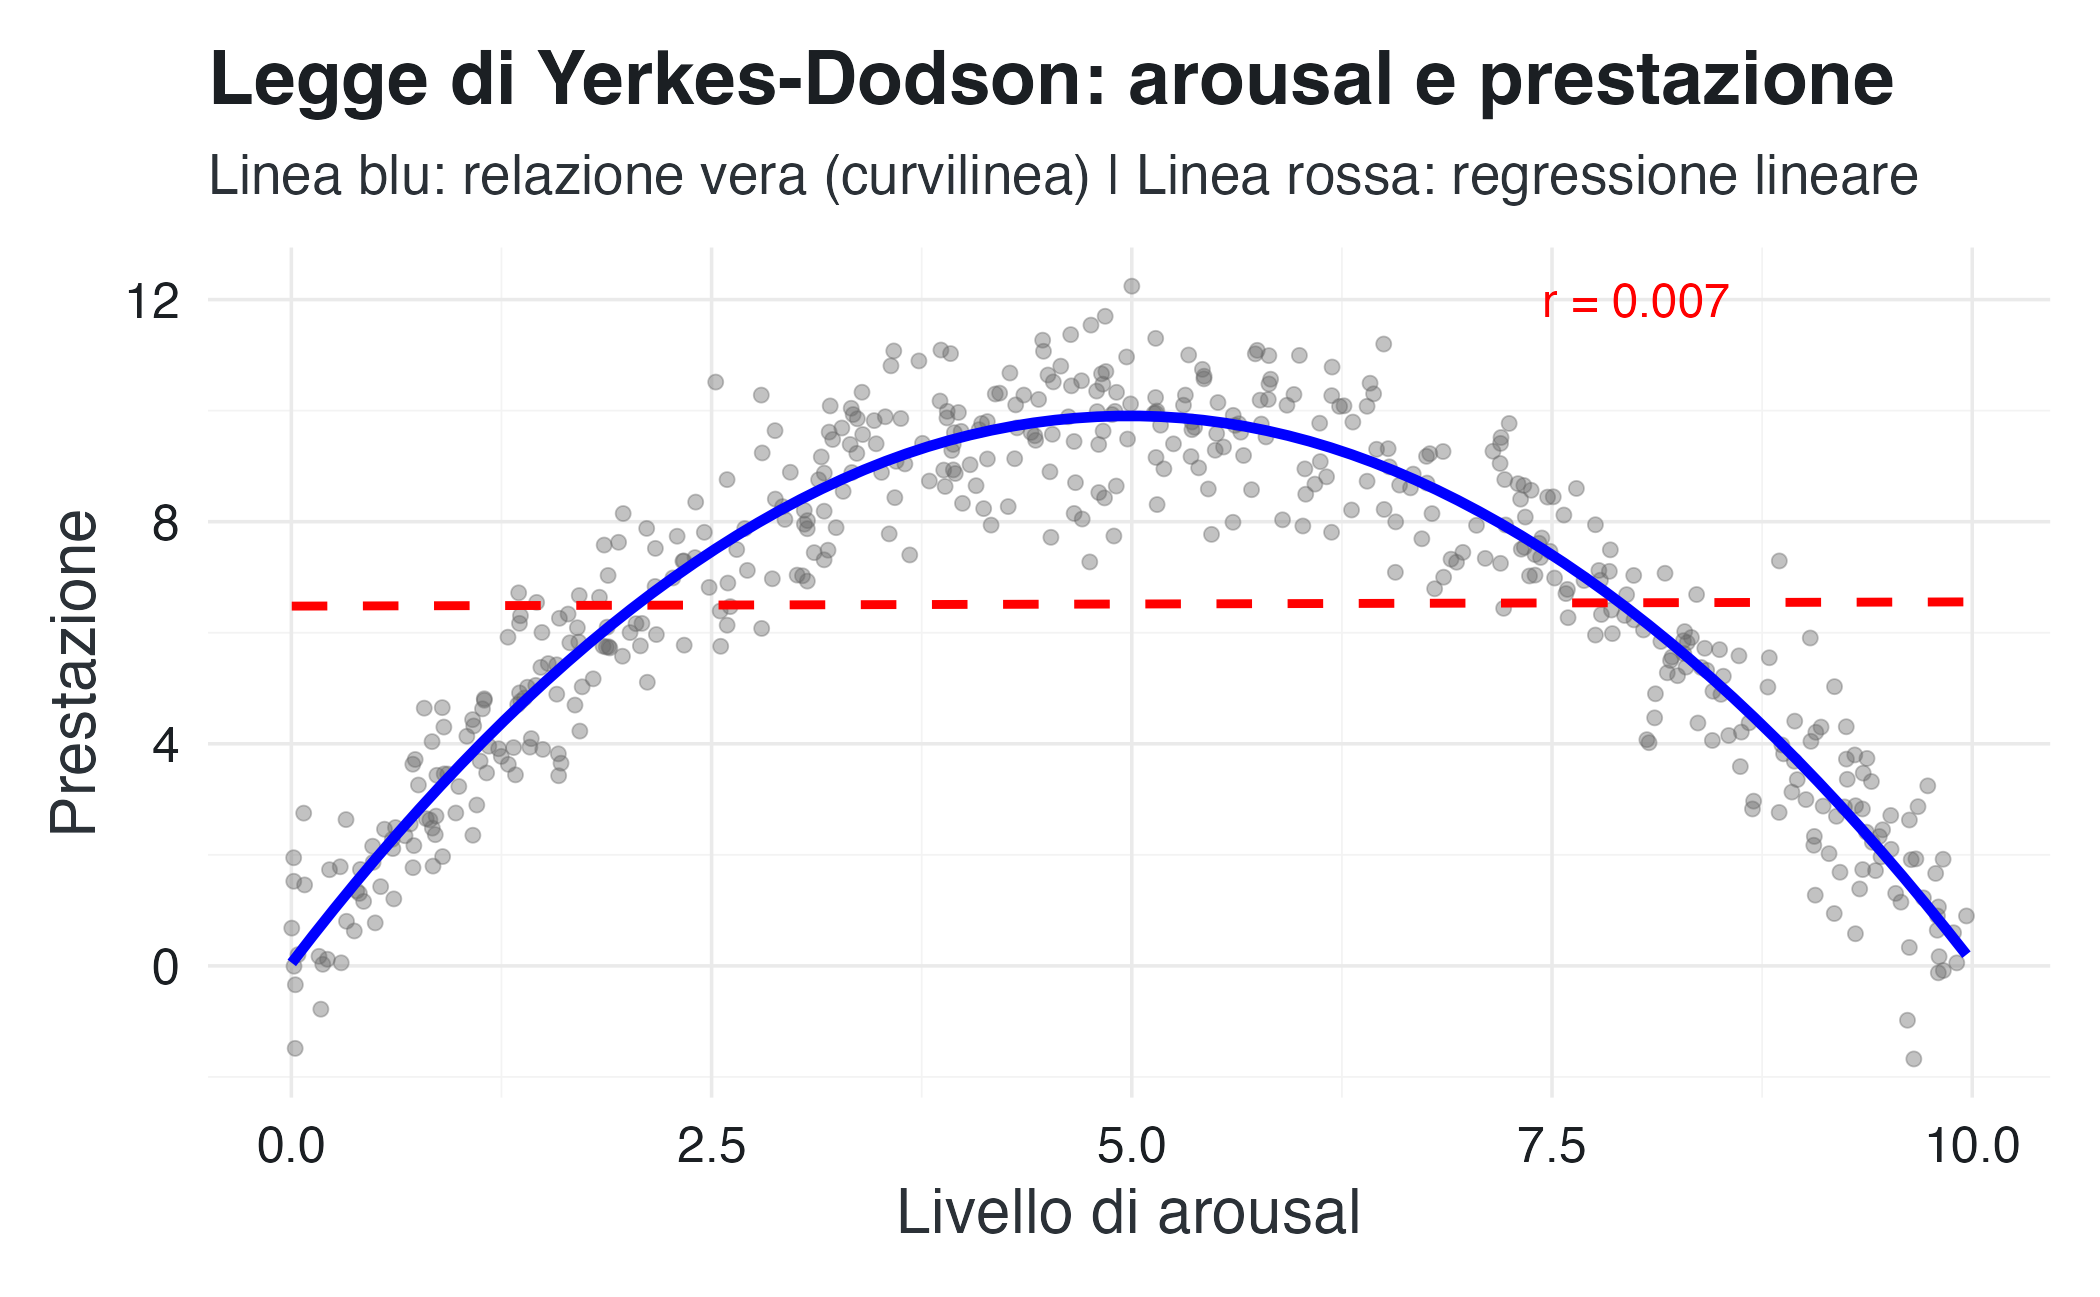
\includegraphics[width=0.85\linewidth,height=\textheight,keepaspectratio]{chapters/probability/09_cov_cor_files/figure-pdf/unnamed-chunk-5-1.png}

}

\caption{Legge di Yerkes-Dodson: relazione curvilinea tra arousal e
prestazione. La correlazione lineare è quasi nulla nonostante la forte
dipendenza.}

\end{figure}%

\begin{Shaded}
\begin{Highlighting}[]
\FunctionTok{cat}\NormalTok{(}\StringTok{"Correlazione lineare (Pearson): r ="}\NormalTok{, }\FunctionTok{round}\NormalTok{(r\_lineare, }\DecValTok{3}\NormalTok{), }\StringTok{"}\SpecialCharTok{\textbackslash{}n}\StringTok{"}\NormalTok{)}
\CommentTok{\#\textgreater{} Correlazione lineare (Pearson): r = 0.007}
\FunctionTok{cat}\NormalTok{(}\StringTok{"Correlazione non lineare (Spearman): ρ ="}\NormalTok{, }\FunctionTok{round}\NormalTok{(}\FunctionTok{cor}\NormalTok{(arousal, prestazione, }\AttributeTok{method =} \StringTok{"spearman"}\NormalTok{), }\DecValTok{3}\NormalTok{), }\StringTok{"}\SpecialCharTok{\textbackslash{}n}\StringTok{"}\NormalTok{)}
\CommentTok{\#\textgreater{} Correlazione non lineare (Spearman): ρ = 0.028}
\end{Highlighting}
\end{Shaded}

\textbf{Interpretazione clinica}: un terapeuta che valutasse solo la
correlazione lineare potrebbe concludere erroneamente che ``non vi sia
alcuna relazione''. In realtà, la relazione è forte ma curvilinea: sia
livelli troppo bassi che troppo alti di ansia compromettono la
prestazione. L'obiettivo non è eliminare l'ansia, ma modularla.

\section{Covarianza nell'inferenza
bayesiana}\label{sec-covariance-in-bayes}

Nell'inferenza bayesiana, la covarianza diventa parte integrante della
rappresentazione delle nostre credenze sui parametri.

\subsection{Covarianza a priori}\label{covarianza-a-priori}

Prima di osservare i dati, possiamo specificare una distribuzione a
priori che includa una struttura di covarianza, riflettendo assunzioni
teoriche sulle relazioni tra i parametri.

\begin{Shaded}
\begin{Highlighting}[]
\NormalTok{mu\_prior }\OtherTok{\textless{}{-}} \FunctionTok{c}\NormalTok{(}\DecValTok{0}\NormalTok{, }\DecValTok{0}\NormalTok{)}
\NormalTok{Sigma\_prior }\OtherTok{\textless{}{-}} \FunctionTok{matrix}\NormalTok{(}\FunctionTok{c}\NormalTok{(}\DecValTok{1}\NormalTok{, }\FloatTok{0.7}\NormalTok{, }\FloatTok{0.7}\NormalTok{, }\DecValTok{1}\NormalTok{), }\AttributeTok{nrow =} \DecValTok{2}\NormalTok{)}

\FunctionTok{set.seed}\NormalTok{(}\DecValTok{123}\NormalTok{)}
\NormalTok{samples\_prior }\OtherTok{\textless{}{-}} \FunctionTok{mvrnorm}\NormalTok{(}\DecValTok{1000}\NormalTok{, mu\_prior, Sigma\_prior)}

\FunctionTok{ggplot}\NormalTok{(}\FunctionTok{as.data.frame}\NormalTok{(samples\_prior), }\FunctionTok{aes}\NormalTok{(}\AttributeTok{x =}\NormalTok{ V1, }\AttributeTok{y =}\NormalTok{ V2)) }\SpecialCharTok{+}
  \FunctionTok{geom\_point}\NormalTok{(}\AttributeTok{alpha =} \FloatTok{0.4}\NormalTok{) }\SpecialCharTok{+}
  \FunctionTok{labs}\NormalTok{(}
    \AttributeTok{title =} \StringTok{"Prior multivariata con correlazione 0.7"}\NormalTok{,}
    \AttributeTok{subtitle =} \StringTok{"Credenze iniziali sulla relazione tra parametri"}\NormalTok{,}
    \AttributeTok{x =} \FunctionTok{expression}\NormalTok{(theta[}\DecValTok{1}\NormalTok{]),}
    \AttributeTok{y =} \FunctionTok{expression}\NormalTok{(theta[}\DecValTok{2}\NormalTok{])}
\NormalTok{  )}
\end{Highlighting}
\end{Shaded}

\begin{center}
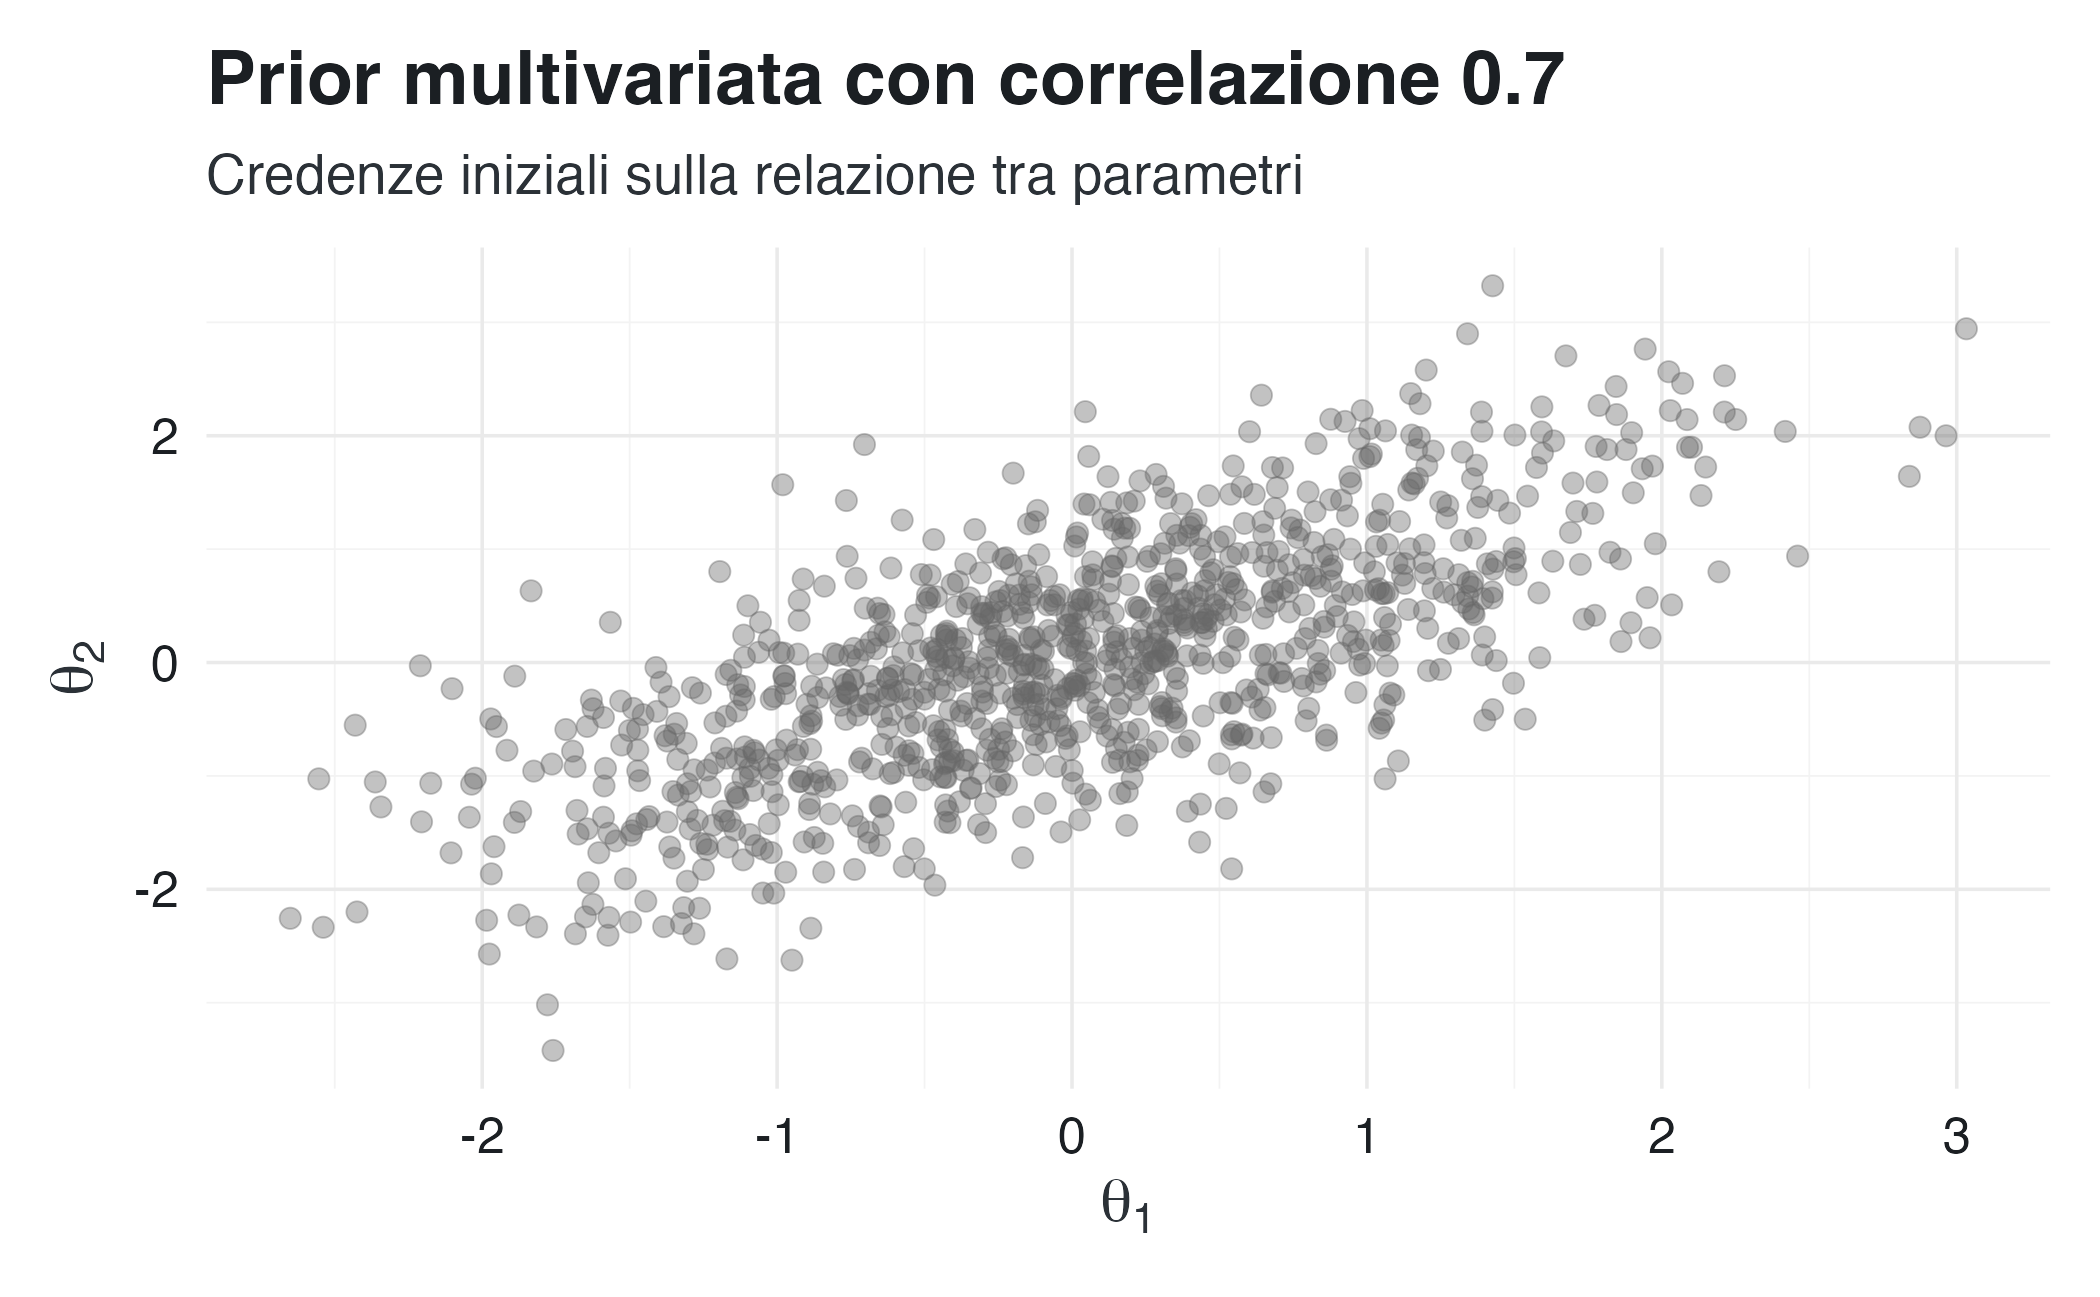
\includegraphics[width=0.85\linewidth,height=\textheight,keepaspectratio]{chapters/probability/09_cov_cor_files/figure-pdf/unnamed-chunk-7-1.png}
\end{center}

Specificare una correlazione positiva nella prior equivale ad affermare
che valori elevati di un parametro tendono ad accompagnarsi a valori
elevati dell'altro.

\subsection{Covarianza a posteriori}\label{covarianza-a-posteriori}

Dopo l'osservazione dei dati, la distribuzione a posteriori presenta una
propria struttura di covarianza che rappresenta lo stato aggiornato
delle credenze.

\subsection{Ponte applicativo}\label{ponte-applicativo-1}

In un modello di regressione, la covarianza \emph{a posteriori} tra i
parametri (ad esempio, intercetta e pendenza) rivela come le incertezze
sui singoli parametri sono correlate. Una covarianza negativa (comune
quando il predittore non è centrato) indica che una sovrastima
dell'intercetta tende ad associarsi a una sottostima della pendenza.

Questa informazione è essenziale per:

\begin{itemize}
\tightlist
\item
  costruire intervalli di credibilità congiunti;
\item
  propagare correttamente l'incertezza nelle previsioni;
\item
  valutare l'identificabilità del modello.
\end{itemize}

\section*{Riflessioni conclusive}\label{riflessioni-conclusive-8}

\markright{Riflessioni conclusive}

La covarianza e la correlazione sono strumenti fondamentali per
quantificare la relazione lineare tra due variabili. Emergono
naturalmente dalla distribuzione congiunta e ne forniscono una sintesi
numerica utile, ma inevitabilmente parziale.

Per lo psicologo clinico e il ricercatore, questi concetti hanno utilità
pratica immediata:

\begin{itemize}
\tightlist
\item
  \textbf{validazione degli strumenti}: correlazioni misurano validità
  convergente e discriminante;
\item
  \textbf{studio delle differenze individuali}: quantificano
  associazioni tra tratti e comportamenti;
\item
  \textbf{pratica clinica}: informano sulle aspettative di comorbidità;
\item
  \textbf{modellazione statistica}: la matrice di covarianza è il cuore
  di regressione, analisi fattoriale e modelli a equazioni strutturali.
\end{itemize}

Un avvertimento cruciale: covarianza e correlazione catturano
\textbf{soltanto la componente lineare} della relazione. L'esempio di
Yerkes-Dodson mostra come associazioni psicologicamente significative
possano rimanere nascoste. Per un'analisi solida, l'esplorazione
numerica deve sempre essere affiancata da un'attenta
\textbf{visualizzazione dei dati}.

\section*{Punti chiave da ricordare}\label{punti-chiave-da-ricordare-8}
\addcontentsline{toc}{section}{Punti chiave da ricordare}

\markright{Punti chiave da ricordare}

\begin{tcolorbox}[enhanced jigsaw, arc=.35mm, bottomrule=.15mm, bottomtitle=1mm, breakable, colback=white, colbacktitle=quarto-callout-important-color!10!white, colframe=quarto-callout-important-color-frame, coltitle=black, left=2mm, leftrule=.75mm, opacityback=0, opacitybacktitle=0.6, rightrule=.15mm, title=\textcolor{quarto-callout-important-color}{\faExclamation}\hspace{0.5em}{Importante}, titlerule=0mm, toprule=.15mm, toptitle=1mm]

\begin{enumerate}
\def\labelenumi{\arabic{enumi}.}
\tightlist
\item
  \textbf{Dalle tabelle discrete alle densità congiunte}

  \begin{itemize}
  \tightlist
  \item
    \(f(x,y)\) è la densità congiunta per variabili continue.
  \item
    Regole di somma e prodotto: somme sostituite da integrali.
  \item
    La distribuzione congiunta contiene tutta l'informazione.
  \end{itemize}
\item
  \textbf{Covarianza come misura della co-variazione lineare}

  \begin{itemize}
  \tightlist
  \item
    \(\text{Cov}(X,Y) = \mathbb{E}[(X-\mu_X)(Y-\mu_Y)]\).
  \item
    Positiva: valori alti insieme, bassi insieme.
  \item
    Negativa: valori alti con bassi.
  \item
    Nulla: assenza di relazione lineare.
  \end{itemize}
\item
  \textbf{Formula computazionale}

  \begin{itemize}
  \tightlist
  \item
    \(\text{Cov}(X,Y) = \mathbb{E}[XY] - \mathbb{E}[X]\mathbb{E}[Y]\).
  \end{itemize}
\item
  \textbf{Correlazione come standardizzazione}

  \begin{itemize}
  \tightlist
  \item
    \(\rho(X,Y) = \text{Cov}(X,Y)/(\sigma_X \sigma_Y)\).
  \item
    Sempre \(-1 \leq \rho \leq 1\).
  \item
    Permette confronti tra scale diverse.
  \end{itemize}
\item
  \textbf{Incorrelazione ≠ indipendenza}

  \begin{itemize}
  \tightlist
  \item
    Indipendenza \(\Rightarrow\) incorrelazione.
  \item
    Incorrelazione \(\not\Rightarrow\) indipendenza.
  \item
    Esempio: legge di Yerkes-Dodson.
  \end{itemize}
\item
  \textbf{Varianza della somma}

  \begin{itemize}
  \tightlist
  \item
    \(\text{Var}(X+Y) = \text{Var}(X) + \text{Var}(Y) + 2\text{Cov}(X,Y)\).
  \item
    Spiega perché le scale composite sono più affidabili.
  \end{itemize}
\end{enumerate}

\textbf{Formule da ricordare:}

\[
\text{Cov}(X,Y) = \mathbb{E}[XY] - \mathbb{E}[X]\mathbb{E}[Y]
\]

\[
\rho(X,Y) = \frac{\text{Cov}(X,Y)}{\sigma_X \sigma_Y}
\]

\[
\text{Var}(X + Y) = \text{Var}(X) + \text{Var}(Y) + 2\text{Cov}(X,Y)
\]

\textbf{Per il prossimo capitolo:}

Nel Capitolo~\ref{sec-prob-inference-uncertainty} passeremo
all'\textbf{inferenza statistica}, presentando la distribuzione
campionaria, l'errore standard e il teorema del limite centrale. Questi
concetti rappresentano il ponte tra la probabilità e l'inferenza
bayesiana.

\end{tcolorbox}

\begin{tcolorbox}[enhanced jigsaw, arc=.35mm, bottomrule=.15mm, bottomtitle=1mm, breakable, colback=white, colbacktitle=quarto-callout-note-color!10!white, colframe=quarto-callout-note-color-frame, coltitle=black, left=2mm, leftrule=.75mm, opacityback=0, opacitybacktitle=0.6, rightrule=.15mm, title=\textcolor{quarto-callout-note-color}{\faInfo}\hspace{0.5em}{Informazioni sull'ambiente di sviluppo}, titlerule=0mm, toprule=.15mm, toptitle=1mm]

\begin{Shaded}
\begin{Highlighting}[]
\FunctionTok{sessionInfo}\NormalTok{()}
\CommentTok{\#\textgreater{} R version 4.6.1 (2026{-}06{-}24)}
\CommentTok{\#\textgreater{} Platform: aarch64{-}apple{-}darwin23}
\CommentTok{\#\textgreater{} Running under: macOS Tahoe 26.5.2}
\CommentTok{\#\textgreater{} }
\CommentTok{\#\textgreater{} Matrix products: default}
\CommentTok{\#\textgreater{} BLAS:   /Library/Frameworks/R.framework/Versions/4.6/Resources/lib/libRblas.0.dylib }
\CommentTok{\#\textgreater{} LAPACK: /Library/Frameworks/R.framework/Versions/4.6/Resources/lib/libRlapack.dylib;  LAPACK version 3.12.1}
\CommentTok{\#\textgreater{} }
\CommentTok{\#\textgreater{} locale:}
\CommentTok{\#\textgreater{} [1] C.UTF{-}8/UTF{-}8/C.UTF{-}8/C/C.UTF{-}8/C.UTF{-}8}
\CommentTok{\#\textgreater{} }
\CommentTok{\#\textgreater{} time zone: Europe/Rome}
\CommentTok{\#\textgreater{} tzcode source: internal}
\CommentTok{\#\textgreater{} }
\CommentTok{\#\textgreater{} attached base packages:}
\CommentTok{\#\textgreater{} [1] stats     graphics  grDevices utils     datasets  methods   base     }
\CommentTok{\#\textgreater{} }
\CommentTok{\#\textgreater{} other attached packages:}
\CommentTok{\#\textgreater{}  [1] ggExtra\_0.11.0        viridis\_0.6.5         viridisLite\_0.4.3    }
\CommentTok{\#\textgreater{}  [4] MASS\_7.3{-}65           ragg\_1.5.2            tinytable\_0.17.0     }
\CommentTok{\#\textgreater{}  [7] withr\_3.0.3           systemfonts\_1.3.2     patchwork\_1.3.2      }
\CommentTok{\#\textgreater{} [10] ggdist\_3.3.3          tidybayes\_3.0.7       bayesplot\_1.15.0     }
\CommentTok{\#\textgreater{} [13] ggplot2\_4.0.3         reliabilitydiag\_0.2.1 priorsense\_1.2.0     }
\CommentTok{\#\textgreater{} [16] posterior\_1.7.0       loo\_2.10.0            rstan\_2.32.7         }
\CommentTok{\#\textgreater{} [19] StanHeaders\_2.32.10   brms\_2.23.0           Rcpp\_1.1.2           }
\CommentTok{\#\textgreater{} [22] sessioninfo\_1.2.4     conflicted\_1.2.0      janitor\_2.2.1        }
\CommentTok{\#\textgreater{} [25] matrixStats\_1.5.0     modelr\_0.1.11         tibble\_3.3.1         }
\CommentTok{\#\textgreater{} [28] dplyr\_1.2.1           tidyr\_1.3.2           rio\_1.3.0            }
\CommentTok{\#\textgreater{} [31] here\_1.0.2           }
\CommentTok{\#\textgreater{} }
\CommentTok{\#\textgreater{} loaded via a namespace (and not attached):}
\CommentTok{\#\textgreater{}  [1] gridExtra\_2.3.1       inline\_0.3.21         rlang\_1.3.0          }
\CommentTok{\#\textgreater{}  [4] magrittr\_2.0.5        snakecase\_0.11.1      otel\_0.2.0           }
\CommentTok{\#\textgreater{}  [7] compiler\_4.6.1        mgcv\_1.9{-}4            vctrs\_0.7.3          }
\CommentTok{\#\textgreater{} [10] stringr\_1.6.0         pkgconfig\_2.0.3       arrayhelpers\_1.1{-}1   }
\CommentTok{\#\textgreater{} [13] fastmap\_1.2.0         backports\_1.5.1       labeling\_0.4.3       }
\CommentTok{\#\textgreater{} [16] promises\_1.5.0        rmarkdown\_2.31        purrr\_1.2.2          }
\CommentTok{\#\textgreater{} [19] xfun\_0.60             cachem\_1.1.0          jsonlite\_2.0.0       }
\CommentTok{\#\textgreater{} [22] later\_1.4.8           broom\_1.0.13          parallel\_4.6.1       }
\CommentTok{\#\textgreater{} [25] R6\_2.6.1              stringi\_1.8.7         RColorBrewer\_1.1{-}3   }
\CommentTok{\#\textgreater{} [28] lubridate\_1.9.5       estimability\_2.0.0    knitr\_1.51           }
\CommentTok{\#\textgreater{} [31] splines\_4.6.1         httpuv\_1.6.17         Matrix\_1.7{-}5         }
\CommentTok{\#\textgreater{} [34] timechange\_0.4.0      tidyselect\_1.2.1      abind\_1.4{-}8          }
\CommentTok{\#\textgreater{} [37] yaml\_2.3.12           codetools\_0.2{-}20      miniUI\_0.1.2         }
\CommentTok{\#\textgreater{} [40] curl\_7.1.0            pkgbuild\_1.4.8        lattice\_0.22{-}9       }
\CommentTok{\#\textgreater{} [43] shiny\_1.14.0          bridgesampling\_1.2{-}1  S7\_0.2.2             }
\CommentTok{\#\textgreater{} [46] coda\_0.19{-}4.1         evaluate\_1.0.5        isoband\_0.3.0        }
\CommentTok{\#\textgreater{} [49] RcppParallel\_5.1.11{-}2 pillar\_1.11.1         tensorA\_0.36.2.1     }
\CommentTok{\#\textgreater{} [52] checkmate\_2.3.4       stats4\_4.6.1          distributional\_0.8.1 }
\CommentTok{\#\textgreater{} [55] generics\_0.1.4        rprojroot\_2.1.1       rstantools\_2.6.0     }
\CommentTok{\#\textgreater{} [58] scales\_1.4.0          xtable\_1.8{-}8          glue\_1.8.1           }
\CommentTok{\#\textgreater{} [61] emmeans\_2.0.3         tools\_4.6.1           mvtnorm\_1.4{-}1        }
\CommentTok{\#\textgreater{} [64] grid\_4.6.1            QuickJSR\_1.10.0       nlme\_3.1{-}169         }
\CommentTok{\#\textgreater{} [67] cli\_3.6.6             textshaping\_1.0.5     svUnit\_1.0.8         }
\CommentTok{\#\textgreater{} [70] Brobdingnag\_1.2{-}9     V8\_8.2.0              gtable\_0.3.6         }
\CommentTok{\#\textgreater{} [73] digest\_0.6.39         farver\_2.1.2          memoise\_2.0.1        }
\CommentTok{\#\textgreater{} [76] htmltools\_0.5.9       lifecycle\_1.0.5       mime\_0.13}
\end{Highlighting}
\end{Shaded}

\end{tcolorbox}

\part{PARTE 3: Distribuzioni specifiche}

\chapter{Introduzione alle distribuzioni di
probabilità}\label{sec-prob-intro-distr}

\section*{Introduzione}\label{introduzione-9}

\markright{Introduzione}

Uno psicologo sta progettando uno studio sui tempi di reazione in un
compito di decisione lessicale. Sa che i tempi di reazione sono sempre
positivi, spesso asimmetrici verso destra e talvolta presentano valori
estremi. Se usasse una distribuzione normale, assegnerebbe densità anche
a tempi negativi, che sono impossibili. Una distribuzione gamma, invece,
rispetterebbe il vincolo di positività e permetterebbe l'asimmetria.

In un altro contesto, una ricercatrice clinica vuole ragionare sulla
probabilità che un paziente raggiunga la remissione dopo un trattamento.
In questo caso, la quantità di interesse è una probabilità, quindi deve
essere compresa tra 0 e 1. Una distribuzione beta è progettata proprio
per rappresentare l'incertezza su quantità di questo tipo.

Questi esempi mostrano perché le distribuzioni di probabilità sono
necessarie. Una distribuzione non è soltanto una curva da disegnare su
un grafico, ma un modo compatto per indicare quali valori sono
possibili, quali sono più plausibili, quanta variabilità ci si può
aspettare e quali assunzioni si fanno sul fenomeno.

Nei capitoli precedenti abbiamo introdotto le variabili casuali, le
funzioni di probabilità e densità, il valore atteso, la varianza, la
covarianza e la correlazione. In questo capitolo facciamo un passo
ulteriore: introduciamo le \textbf{famiglie parametriche di
distribuzioni}, ovvero il vocabolario standard con cui costruire modelli
probabilistici.

Lo scopo del capitolo è soprattutto orientativo. Non studieremo ancora
nel dettaglio ogni distribuzione: questo sarà il compito dei capitoli
successivi. In questo capitolo impareremo a riconoscere il ruolo
generale delle distribuzioni, a distinguere le distribuzioni discrete da
quelle continue e a scegliere, in modo ragionato, la famiglia di
distribuzioni più appropriata per una determinata domanda di ricerca.

\begin{tcolorbox}[enhanced jigsaw, arc=.35mm, bottomrule=.15mm, bottomtitle=1mm, breakable, colback=white, colbacktitle=quarto-callout-tip-color!10!white, colframe=quarto-callout-tip-color-frame, coltitle=black, left=2mm, leftrule=.75mm, opacityback=0, opacitybacktitle=0.6, rightrule=.15mm, title=\textcolor{quarto-callout-tip-color}{\faLightbulb}\hspace{0.5em}{Prerequisiti}, titlerule=0mm, toprule=.15mm, toptitle=1mm]

Per seguire questo capitolo è necessario aver letto:

\begin{itemize}
\tightlist
\item
  Capitolo~\ref{sec-prob-random-var};
\item
  Capitolo~\ref{sec-prob-distr};
\item
  Capitolo~\ref{sec-prob-random-var-properties};
\item
  Capitolo~\ref{sec-prob-cov-cor}, almeno per l'idea che le variabili
  casuali possano variare insieme.
\end{itemize}

Questo capitolo apre la Parte 3 di questo modulo di richiamo. Il suo
ruolo è preparare lo studio delle distribuzioni discrete nel 2 e delle
distribuzioni continue nel Capitolo~\ref{sec-prob-cont-distr}.

Conoscenze matematiche utili:

\begin{itemize}
\tightlist
\item
  Appendice~\ref{sec-apx-combinatorics}, per le distribuzioni discrete
  basate su conteggi;
\item
  Appendice~\ref{sec-apx-calculus}, per comprendere le densità continue
  e l'integrazione.
\end{itemize}

\end{tcolorbox}

\begin{tcolorbox}[enhanced jigsaw, arc=.35mm, bottomrule=.15mm, bottomtitle=1mm, breakable, colback=white, colbacktitle=quarto-callout-caution-color!10!white, colframe=quarto-callout-caution-color-frame, coltitle=black, left=2mm, leftrule=.75mm, opacityback=0, opacitybacktitle=0.6, rightrule=.15mm, title=\textcolor{quarto-callout-caution-color}{\faFire}\hspace{0.5em}{Preparazione del Notebook}, titlerule=0mm, toprule=.15mm, toptitle=1mm]

\begin{Shaded}
\begin{Highlighting}[]
\NormalTok{here}\SpecialCharTok{::}\FunctionTok{here}\NormalTok{(}\StringTok{"code"}\NormalTok{, }\StringTok{"\_common.R"}\NormalTok{) }\SpecialCharTok{|\textgreater{}} 
  \FunctionTok{source}\NormalTok{()}
\FunctionTok{apply\_visual\_theme}\NormalTok{()}
\end{Highlighting}
\end{Shaded}

\end{tcolorbox}

\section{Perché servono le distribuzioni}\label{sec-why-distributions}

\subsection{Dalle variabili casuali alle famiglie di
distribuzioni}\label{dalle-variabili-casuali-alle-famiglie-di-distribuzioni}

Una variabile casuale rappresenta una quantità incerta, come una
risposta corretta o errata, il numero di sintomi riportati, il tempo di
reazione o il punteggio ottenuto su una scala psicometrica. La
distribuzione di probabilità specifica come la probabilità o la densità
sono assegnate ai valori possibili di quella variabile.

Tuttavia, nella pratica scientifica non costruiamo ogni distribuzione da
zero. Utilizziamo famiglie già note, ciascuna con proprietà matematiche
e interpretative ben comprese. La distribuzione normale, la binomiale,
la Poisson, la beta e la gamma sono esempi di \textbf{famiglie
parametriche}.

Una famiglia parametrica è un insieme di distribuzioni accomunate dalla
stessa forma generale, ma differenziate da uno o più \textbf{parametri}.
Ad esempio:

\begin{itemize}
\tightlist
\item
  la famiglia normale è determinata da una media \(\mu\) e da una
  deviazione standard \(\sigma\);
\item
  la famiglia binomiale è determinata dal numero di prove \(n\) e dalla
  probabilità di successo \(p\);
\item
  la famiglia beta è determinata da due parametri di forma, spesso
  indicati con \(\alpha\) e \(\beta\);
\item
  la famiglia di Poisson è determinata da un tasso medio \(\lambda\).
\end{itemize}

Specificare una famiglia significa decidere la \textbf{forma generale}
del modello. Specificare i valori dei parametri significa scegliere una
distribuzione particolare all'interno di quella famiglia.

\begin{tcolorbox}[enhanced jigsaw, arc=.35mm, bottomrule=.15mm, bottomtitle=1mm, breakable, colback=white, colbacktitle=quarto-callout-note-color!10!white, colframe=quarto-callout-note-color-frame, coltitle=black, left=2mm, leftrule=.75mm, opacityback=0, opacitybacktitle=0.6, rightrule=.15mm, title=\textcolor{quarto-callout-note-color}{\faInfo}\hspace{0.5em}{Parametro della distribuzione e parametro inferenziale}, titlerule=0mm, toprule=.15mm, toptitle=1mm]

Nei capitoli sulle distribuzioni, un parametro può essere considerato
come un dato numerico, ad esempio una distribuzione normale con
\(\mu = 100\) e \(\sigma = 15\). Questo permette di studiare le
proprietà della distribuzione.

Nell'inferenza bayesiana, invece, molti parametri sono quantità ignote
su cui abbiamo incertezza. Ad esempio, la probabilità di remissione
\(\theta\) può essere il parametro di un modello binomiale, ma anche una
quantità su cui vogliamo costruire una distribuzione a priori e, dopo i
dati, una distribuzione a posteriori. Questa distinzione sarà centrale
nella Parte 4.

\end{tcolorbox}

\subsection{Le distribuzioni come rappresentazioni
dell'incertezza}\label{le-distribuzioni-come-rappresentazioni-dellincertezza}

Nel ragionamento bayesiano, una distribuzione di probabilità è prima di
tutto uno strumento per rappresentare l'incertezza. Può rappresentare
l'incertezza relativa a un'osservazione futura, a un parametro
sconosciuto o a una quantità derivata da un modello.

Consideriamo, ad esempio, la proporzione \(\theta\) di studenti
universitari con sintomi d'ansia clinicamente rilevanti. Dire ``credo
che sia il 25\%'' è una credenza puntuale. Spesso, però, non vogliamo
attribuire tutta la nostra credenza a un singolo valore. Potremmo
ritenere plausibili valori compresi tra 0.20 e 0.30, meno plausibili
valori intorno a 0.10 o 0.45, e quasi impossibili valori superiori a
0.70. Una distribuzione su \(\theta\) rende esplicita questa struttura
graduata di credenze.

Questa rappresentazione è più informativa di una stima puntuale, in
quanto comunica anche la \textbf{dispersione} della nostra incertezza.
Due ricercatori possono avere la stessa stima centrale, ad esempio 0.25,
ma gradi di incertezza molto diversi: uno potrebbe essere quasi certo
che il valore sia vicino a 0.25, mentre l'altro potrebbe considerare
plausibile un intervallo molto ampio di valori.

\subsection{Le distribuzioni come modelli della
variabilità}\label{le-distribuzioni-come-modelli-della-variabilituxe0}

Le distribuzioni servono anche a rappresentare la variabilità dei dati.
In psicologia, la variabilità è spesso una componente essenziale del
fenomeno: le persone rispondono in modo diverso allo stesso trattamento,
lo stesso individuo può cambiare nel tempo e contesti diversi possono
influenzare il comportamento osservato.

Per questo motivo, modellare soltanto la media può non essere
sufficiente. Una distribuzione permette di rappresentare non solo il
centro dei dati, ma anche la dispersione, l'asimmetria, le code e,
quando necessario, la presenza di sottogruppi. In questo senso, la
variabilità non è semplicemente rumore, ma informazione.

Come discusso da Segal et al. (\citeproc{ref-segal2025embracing}{2025}),
molti fenomeni psicologici e psicopatologici sono caratterizzati da
un'eterogeneità sostanziale. Le distribuzioni di probabilità forniscono
un linguaggio per rendere visibile e modellabile questa eterogeneità.

\section{Tre domande per scegliere una
distribuzione}\label{sec-three-questions-distributions}

La scelta di una distribuzione non dovrebbe partire dalla domanda
``Quale curva assomiglia al mio istogramma?''. Questa domanda può essere
utile, ma viene dopo. Prima è necessario chiarire che cosa si sta
modellando e quali valori sono logicamente possibili.

\subsection{1. Che tipo di quantità sto
modellando?}\label{che-tipo-di-quantituxe0-sto-modellando}

La prima distinzione riguarda la natura della quantità:

\begin{itemize}
\tightlist
\item
  un \textbf{evento binario}, come risposta corretta/errata o remissione
  sì/no;
\item
  un \textbf{conteggio}, come numero di sintomi, errori o episodi;
\item
  una \textbf{proporzione} o probabilità, vincolata tra 0 e 1;
\item
  una \textbf{misura continua}, come un tempo di reazione o un punteggio
  psicometrico;
\item
  un \textbf{tasso}, come il numero medio di eventi per unità di tempo;
\item
  una \textbf{varianza} o una deviazione standard, sempre non negativa.
\end{itemize}

Questa classificazione restringe subito l'insieme delle distribuzioni
plausibili.

\subsection{2. Qual è il supporto della
quantità?}\label{qual-uxe8-il-supporto-della-quantituxe0}

Il \textbf{supporto} è l'insieme dei valori che una variabile può
assumere. Una distribuzione appropriata deve assegnare probabilità solo
ai valori compatibili con il fenomeno.

{\def\LTcaptype{none} % do not increment counter
\begin{longtable}[]{@{}
  >{\raggedright\arraybackslash}p{(\linewidth - 6\tabcolsep) * \real{0.2500}}
  >{\raggedright\arraybackslash}p{(\linewidth - 6\tabcolsep) * \real{0.2500}}
  >{\raggedright\arraybackslash}p{(\linewidth - 6\tabcolsep) * \real{0.2500}}
  >{\raggedright\arraybackslash}p{(\linewidth - 6\tabcolsep) * \real{0.2500}}@{}}
\toprule\noalign{}
\begin{minipage}[b]{\linewidth}\raggedright
Quantità da modellare
\end{minipage} & \begin{minipage}[b]{\linewidth}\raggedright
Supporto
\end{minipage} & \begin{minipage}[b]{\linewidth}\raggedright
Famiglie candidate
\end{minipage} & \begin{minipage}[b]{\linewidth}\raggedright
Esempio psicologico
\end{minipage} \\
\midrule\noalign{}
\endhead
\bottomrule\noalign{}
\endlastfoot
Evento binario & \(\{0,1\}\) & Bernoulli & Risposta corretta/errata \\
Numero di successi su \(n\) prove & \(\{0,1,\ldots,n\}\) & Binomiale &
Item corretti su 20 \\
Conteggio non limitato superiormente & \(\{0,1,2,\ldots\}\) & Poisson &
Attacchi di panico in un mese \\
Proporzione o probabilità & \([0,1]\) & Beta & Tasso di remissione \\
Misura continua su tutta la retta & \(\mathbb{R}\) & Normale, \(t\) di
Student, Cauchy & Punteggi standardizzati \\
Quantità positiva continua & \(\mathbb{R}^+\) & Esponenziale, Gamma &
Tempi di reazione, latenze \\
Varianza o precisione & \(\mathbb{R}^+\) & Gamma, chi-quadrato &
Variabilità tra soggetti \\
\end{longtable}
}

Il supporto è un criterio di esclusione molto forte. Se una quantità non
può assumere valori negativi, una distribuzione che assegna densità a
valori negativi deve essere utilizzata con estrema cautela o sostituita
da una famiglia di distribuzioni più adatta.

\subsection{3. Quale forma mi aspetto?}\label{quale-forma-mi-aspetto}

Dopo aver considerato il supporto, si valuta la forma attesa della
distribuzione:

\begin{itemize}
\tightlist
\item
  simmetrica o asimmetrica;
\item
  concentrata o dispersa;
\item
  con code leggere o pesanti;
\item
  con valori estremi frequenti o rari;
\item
  con un solo picco o con più sottogruppi plausibili.
\end{itemize}

La forma non è un dettaglio estetico. Esprime ipotesi sostantive sul
processo che genera i dati o sulla struttura delle nostre credenze. Ad
esempio, l'uso di una distribuzione gamma per i tempi di reazione
suggerisce che i tempi siano positivi e asimmetrici, mentre l'uso di una
distribuzione normale per un punteggio standardizzato suggerisce una
variabilità approssimativamente simmetrica attorno a un centro.

\section{Famiglie parametriche e interpretazione dei
parametri}\label{sec-parametric-families}

\subsection{Posizione, scala e forma}\label{posizione-scala-e-forma}

I parametri di una distribuzione possono avere ruoli diversi. Una
distinzione utile è quella tra parametri di \textbf{posizione},
\textbf{scala} e \textbf{forma}.

Un parametro di posizione indica dove si concentra la distribuzione.
Nella distribuzione normale, il parametro \(\mu\) sposta la curva verso
sinistra o verso destra. Un parametro di scala controlla la dispersione:
nella distribuzione normale, per esempio, \(\sigma\) determina quanto la
distribuzione è ampia. I parametri di forma, infine, modificano
l'asimmetria, le code o la concentrazione: nella distribuzione beta, per
esempio, i parametri \(\alpha\) e \(\beta\) possono produrre
distribuzioni simmetriche, asimmetriche, a U o fortemente concentrate.

\begin{Shaded}
\begin{Highlighting}[]
\NormalTok{x }\OtherTok{\textless{}{-}} \FunctionTok{seq}\NormalTok{(}\SpecialCharTok{{-}}\DecValTok{4}\NormalTok{, }\DecValTok{4}\NormalTok{, }\AttributeTok{length.out =} \DecValTok{400}\NormalTok{)}
\NormalTok{curve\_normali }\OtherTok{\textless{}{-}} \FunctionTok{rbind}\NormalTok{(}
  \FunctionTok{data.frame}\NormalTok{(}\AttributeTok{x =}\NormalTok{ x, }\AttributeTok{density =} \FunctionTok{dnorm}\NormalTok{(x, }\AttributeTok{mean =} \DecValTok{0}\NormalTok{, }\AttributeTok{sd =} \DecValTok{1}\NormalTok{), }\AttributeTok{modello =} \StringTok{"Normale(0, 1)"}\NormalTok{),}
  \FunctionTok{data.frame}\NormalTok{(}\AttributeTok{x =}\NormalTok{ x, }\AttributeTok{density =} \FunctionTok{dnorm}\NormalTok{(x, }\AttributeTok{mean =} \FloatTok{1.5}\NormalTok{, }\AttributeTok{sd =} \DecValTok{1}\NormalTok{), }\AttributeTok{modello =} \StringTok{"Normale(1.5, 1)"}\NormalTok{),}
  \FunctionTok{data.frame}\NormalTok{(}\AttributeTok{x =}\NormalTok{ x, }\AttributeTok{density =} \FunctionTok{dnorm}\NormalTok{(x, }\AttributeTok{mean =} \DecValTok{0}\NormalTok{, }\AttributeTok{sd =} \FloatTok{1.8}\NormalTok{), }\AttributeTok{modello =} \StringTok{"Normale(0, 1.8)"}\NormalTok{)}
\NormalTok{)}

\FunctionTok{ggplot}\NormalTok{(curve\_normali, }\FunctionTok{aes}\NormalTok{(}\AttributeTok{x =}\NormalTok{ x, }\AttributeTok{y =}\NormalTok{ density, }\AttributeTok{linetype =}\NormalTok{ modello)) }\SpecialCharTok{+}
  \FunctionTok{geom\_line}\NormalTok{(}\AttributeTok{linewidth =} \FloatTok{1.1}\NormalTok{) }\SpecialCharTok{+}
  \FunctionTok{labs}\NormalTok{(}
    \AttributeTok{title =} \StringTok{"Effetto dei parametri in una famiglia parametrica"}\NormalTok{,}
    \AttributeTok{subtitle =} \StringTok{"La media modifica la posizione; la deviazione standard modifica la dispersione"}\NormalTok{,}
    \AttributeTok{x =} \StringTok{"Valore"}\NormalTok{,}
    \AttributeTok{y =} \StringTok{"Densità"}\NormalTok{,}
    \AttributeTok{linetype =} \StringTok{"Distribuzione"}
\NormalTok{  )}
\end{Highlighting}
\end{Shaded}

\begin{center}
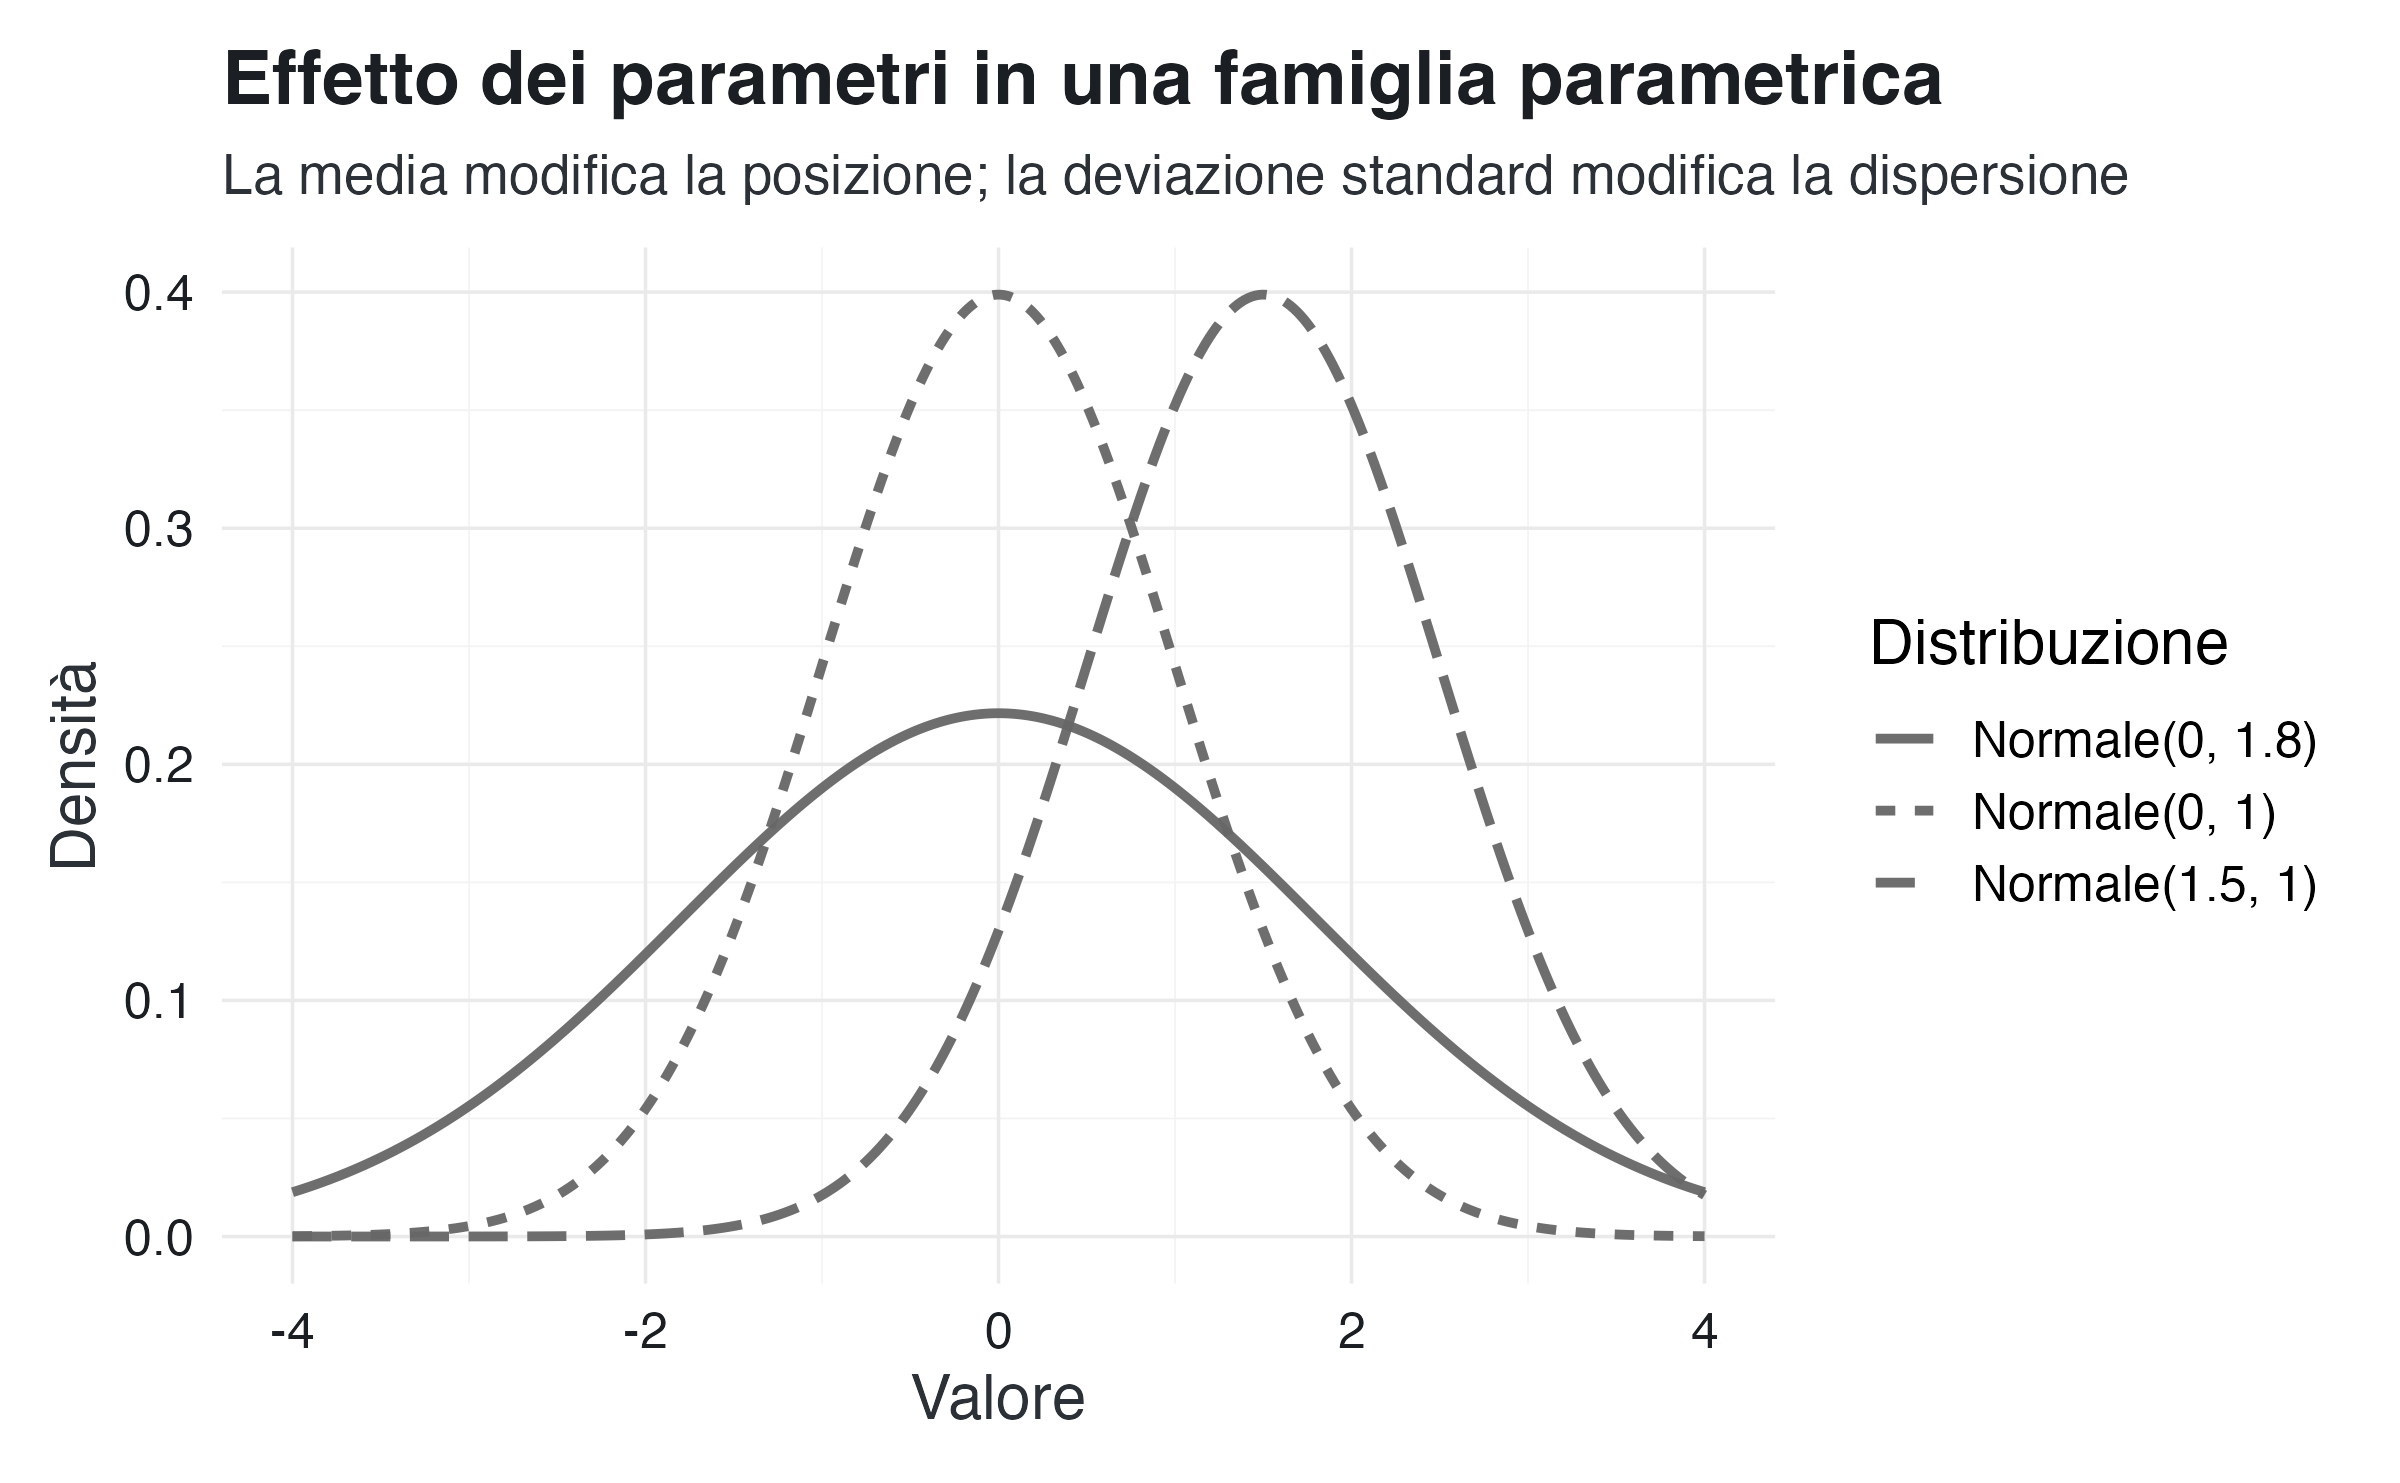
\includegraphics[width=1\linewidth,height=\textheight,keepaspectratio]{chapters/probability/10_intro_distributions_files/figure-pdf/unnamed-chunk-2-1.png}
\end{center}

Lo stesso principio si applica a tutte le famiglie: i parametri non sono
simboli arbitrari, ma strumenti per codificare le assunzioni sulla
quantità che stiamo modellando.

\subsection{Un piccolo lessico
operativo}\label{un-piccolo-lessico-operativo}

Nel seguito del modulo incontreremo spesso le seguenti parole. Conviene
fissarle subito.

\textbf{Supporto}: l'insieme dei valori possibili. Una distribuzione
Beta ha supporto \([0,1]\), mentre una distribuzione di Poisson ha
supporto \(\{0,1,2,\ldots\}\).

\textbf{Massa di probabilità}: per le variabili discrete, è la
probabilità assegnata a ciascun valore specifico, come \(P(X = 3)\).

\textbf{Densità}: per le variabili continue, è una funzione che permette
di calcolare le probabilità su intervalli. Per una variabile continua,
la probabilità che assuma un valore esatto è nulla; ciò che ha senso è
la probabilità che assuma valori compresi tra \(a\) e \(b\).

\textbf{Funzione di distribuzione cumulativa}: la funzione che
restituisce \(P(X \leq x)\).

\textbf{Quantile}: il valore sotto il quale cade una certa probabilità.
Ad esempio, il quantile 0.95 è il valore sotto il quale si trova il 95\%
della distribuzione.

Questi concetti sono già stati introdotti nei capitoli precedenti, ma
diventeranno operativi nei capitoli 11 e 12, in cui useremo anche le
funzioni R associate alle principali distribuzioni.

\section{Il ruolo delle distribuzioni in un modello
bayesiano}\label{sec-distribution-roles-bayes}

Anche se la verosimiglianza e l'aggiornamento bayesiano verranno
trattati in modo sistematico nella Parte 4, è utile anticipare il ruolo
che le distribuzioni avranno in quel contesto.

Un modello bayesiano semplice può essere schematizzato nel modo
seguente:

\[
\theta \sim p(\theta),
\qquad
Y \mid \theta \sim p(y \mid \theta).
\]

La prima riga rappresenta l'incertezza sul parametro \(\theta\) prima
dell'osservazione dei dati. La seconda riga rappresenta il modello
probabilistico dei dati condizionato a un valore del parametro. In
questa forma compatta sono già presenti due usi diversi delle
distribuzioni.

\subsection{Distribuzioni per i parametri:
prior}\label{distribuzioni-per-i-parametri-prior}

Una distribuzione può rappresentare ciò che sappiamo o ciò che non
sappiamo riguardo a un parametro. Per esempio, se \(\theta\) rappresenta
una probabilità di remissione, una distribuzione beta può esprimere le
credenze preliminari su valori compresi tra 0 e 1.

In questa funzione, la distribuzione risponde alla domanda:

\begin{quote}
Quali valori del parametro ritengo plausibili prima di osservare questi
dati?
\end{quote}

\subsection{Distribuzioni per i dati: modello
generativo}\label{distribuzioni-per-i-dati-modello-generativo}

Una distribuzione può anche descrivere come potrebbero essere generati i
dati, a partire da un determinato valore del parametro. Se osserviamo il
numero di remissioni su \(n\) pazienti, una distribuzione binomiale può
rappresentare il numero di successi attesi per un determinato valore di
\(\theta\).

In questa funzione, la distribuzione risponde alla domanda:

\begin{quote}
Se il parametro assumesse questo valore, quali dati mi aspetterei di
osservare?
\end{quote}

\subsection{Distribuzioni predittive}\label{distribuzioni-predittive}

Infine, una distribuzione può descrivere ciò che ci aspettiamo di
osservare in futuro. Nel quadro bayesiano, la previsione tiene conto sia
della variabilità dei dati sia dell'incertezza residua sui parametri.

Questa terza funzione sarà importante più avanti, ma è utile
riconoscerla fin da ora: un modello probabilistico non serve solo a
spiegare dati già osservati, ma anche a formulare aspettative
controllabili su dati futuri.

\begin{tcolorbox}[enhanced jigsaw, arc=.35mm, bottomrule=.15mm, bottomtitle=1mm, breakable, colback=white, colbacktitle=quarto-callout-important-color!10!white, colframe=quarto-callout-important-color-frame, coltitle=black, left=2mm, leftrule=.75mm, opacityback=0, opacitybacktitle=0.6, rightrule=.15mm, title=\textcolor{quarto-callout-important-color}{\faExclamation}\hspace{0.5em}{Idea guida}, titlerule=0mm, toprule=.15mm, toptitle=1mm]

Nel manuale useremo le distribuzioni in tre modi complementari:

\begin{enumerate}
\def\labelenumi{\arabic{enumi}.}
\tightlist
\item
  per descrivere quantità osservabili;
\item
  per rappresentare incertezza sui parametri;
\item
  per prevedere osservazioni future.
\end{enumerate}

La Parte 3 costruisce il vocabolario. La Parte 4 mostrerà come questo
vocabolario diventa inferenza.

\end{tcolorbox}

\section{Mappa delle principali
famiglie}\label{sec-map-distribution-families}

\subsection{Distribuzioni discrete}\label{distribuzioni-discrete}

Le distribuzioni discrete assegnano probabilità a valori separati e
numerabili. Sono naturali quando gli esiti sono categorie, successi,
errori o conteggi.

{\def\LTcaptype{none} % do not increment counter
\begin{longtable}[]{@{}
  >{\raggedright\arraybackslash}p{(\linewidth - 6\tabcolsep) * \real{0.2500}}
  >{\raggedright\arraybackslash}p{(\linewidth - 6\tabcolsep) * \real{0.2500}}
  >{\raggedright\arraybackslash}p{(\linewidth - 6\tabcolsep) * \real{0.2500}}
  >{\raggedright\arraybackslash}p{(\linewidth - 6\tabcolsep) * \real{0.2500}}@{}}
\toprule\noalign{}
\begin{minipage}[b]{\linewidth}\raggedright
Famiglia
\end{minipage} & \begin{minipage}[b]{\linewidth}\raggedright
Quantità modellata
\end{minipage} & \begin{minipage}[b]{\linewidth}\raggedright
Parametri principali
\end{minipage} & \begin{minipage}[b]{\linewidth}\raggedright
Capitolo
\end{minipage} \\
\midrule\noalign{}
\endhead
\bottomrule\noalign{}
\endlastfoot
Uniforme discreta & valori discreti equiprobabili & numero di valori
possibili & 2 \\
Bernoulli & singolo evento binario & probabilità \(p\) & 2 \\
Binomiale & numero di successi in \(n\) prove & \(n\), \(p\) & 2 \\
Poisson & conteggio di eventi in un intervallo & tasso \(\lambda\) &
2 \\
\end{longtable}
}

Esempi psicologici tipici sono la risposta corretta a un item, il numero
di item superati, il numero di comportamenti osservati in una sessione o
il numero di episodi registrati in un periodo.

\subsection{Distribuzioni continue}\label{distribuzioni-continue}

Le distribuzioni continue assegnano densità su intervalli di valori.
Sono naturali per tempi, punteggi, misure fisiologiche, probabilità,
tassi e parametri continui.

{\def\LTcaptype{none} % do not increment counter
\begin{longtable}[]{@{}
  >{\raggedright\arraybackslash}p{(\linewidth - 6\tabcolsep) * \real{0.2500}}
  >{\raggedright\arraybackslash}p{(\linewidth - 6\tabcolsep) * \real{0.2500}}
  >{\raggedright\arraybackslash}p{(\linewidth - 6\tabcolsep) * \real{0.2500}}
  >{\raggedright\arraybackslash}p{(\linewidth - 6\tabcolsep) * \real{0.2500}}@{}}
\toprule\noalign{}
\begin{minipage}[b]{\linewidth}\raggedright
Famiglia
\end{minipage} & \begin{minipage}[b]{\linewidth}\raggedright
Quantità modellata
\end{minipage} & \begin{minipage}[b]{\linewidth}\raggedright
Parametri principali
\end{minipage} & \begin{minipage}[b]{\linewidth}\raggedright
Capitolo
\end{minipage} \\
\midrule\noalign{}
\endhead
\bottomrule\noalign{}
\endlastfoot
Uniforme continua & valori equiplausibili in un intervallo & estremi
\(a\), \(b\) & Capitolo~\ref{sec-prob-cont-distr} \\
Esponenziale & tempi di attesa & tasso \(\lambda\) &
Capitolo~\ref{sec-prob-cont-distr} \\
Normale & misure simmetriche su \(\mathbb{R}\) & \(\mu\), \(\sigma\) &
Capitolo~\ref{sec-prob-cont-distr} \\
Chi-quadrato & somme di quadrati, varianze & gradi di libertà &
Capitolo~\ref{sec-prob-cont-distr} \\
\(t\) di Student & quantità continue con code più pesanti & gradi di
libertà & Capitolo~\ref{sec-prob-cont-distr} \\
Cauchy & distribuzioni molto robuste e a code pesanti & posizione, scala
& Capitolo~\ref{sec-prob-cont-distr} \\
Beta & proporzioni e probabilità & \(\alpha\), \(\beta\) &
Capitolo~\ref{sec-prob-cont-distr} \\
Gamma & tassi, tempi positivi, varianze & forma, tasso o scala &
Capitolo~\ref{sec-prob-cont-distr} \\
\end{longtable}
}

Questa mappa non deve essere memorizzata come una lista chiusa. Serve
piuttosto a sviluppare un'abitudine: prima si guarda alla natura della
quantità, poi al supporto, poi alla forma, infine al ruolo che la
distribuzione deve svolgere nel modello.

\section{Esempi di scelta della
distribuzione}\label{sec-choosing-examples}

\subsection{Remissione clinica: evento binario e
probabilità}\label{remissione-clinica-evento-binario-e-probabilituxe0}

Supponiamo di voler studiare se un paziente raggiunge la remissione dopo
un intervento psicoterapeutico. Per ogni paziente osserviamo un esito
binario: remissione sì/no. La distribuzione naturale per una singola
osservazione è la Bernoulli.

Se invece osserviamo \(y\) remissioni su \(n\) pazienti, la
distribuzione naturale per il conteggio dei successi è la binomiale. Se
vogliamo poi rappresentare l'incertezza sulla probabilità di remissione
\(\theta\), una candidata naturale è la distribuzione Beta, perché
\(\theta\) deve appartenere all'intervallo \([0,1]\).

Qui compaiono tre livelli:

\begin{itemize}
\tightlist
\item
  osservazione singola: Bernoulli;
\item
  conteggio aggregato: Binomiale;
\item
  incertezza sulla probabilità: Beta.
\end{itemize}

La relazione tra questi livelli verrà ripresa nei capitoli successivi.

\subsection{Tempi di reazione: quantità positive e
asimmetriche}\label{tempi-di-reazione-quantituxe0-positive-e-asimmetriche}

I tempi di reazione non possono essere negativi e spesso presentano una
coda lunga verso destra. Per questo motivo, una distribuzione normale
potrebbe non essere adeguata, soprattutto in presenza di un'asimmetria
marcata. Distribuzioni come la gamma o, in altri contesti, la
log-normale rispettano il vincolo di positività e permettono
l'asimmetria.

La scelta non dipende solo dal grafico dei dati. Dipende anche da ciò
che si ritiene plausibile riguardo al processo: un tempo di reazione può
essere considerato come una durata positiva influenzata da molteplici
componenti cognitive, motorie e attentive.

\subsection{Conteggi di eventi: frequenze in un
intervallo}\label{conteggi-di-eventi-frequenze-in-un-intervallo}

Se si conta il numero di attacchi di panico in un mese, il numero di
errori in un compito o il numero di comportamenti osservati in una
sessione, la variabile assume valori interi non negativi. Una
distribuzione naturale è quella di Poisson, soprattutto quando gli
eventi sono relativamente rari e l'intervallo di osservazione è
definito.

Tuttavia, se il tasso medio di eventi varia molto da un individuo
all'altro, la semplice distribuzione di Poisson può risultare troppo
rigida. In seguito vedremo che introdurre incertezza o variabilità nel
tasso può produrre modelli più flessibili.

\subsection{Punteggi psicometrici: continui o quasi
continui?}\label{punteggi-psicometrici-continui-o-quasi-continui}

Molti punteggi psicometrici derivano dalla somma di item discreti, ma
sono spesso trattati come quantità continue quando il numero di
possibili valori è elevato e la distribuzione è approssimativamente
regolare. In questi casi, la normalità può essere una buona
approssimazione operativa.

Tuttavia, la normalità non dovrebbe essere assunta automaticamente. Se
il punteggio è fortemente asimmetrico, limitato inferiormente o
superiormente o presenta accumuli agli estremi, potrebbe essere
necessario un modello diverso.

\begin{tcolorbox}[enhanced jigsaw, arc=.35mm, bottomrule=.15mm, bottomtitle=1mm, breakable, colback=white, colbacktitle=quarto-callout-warning-color!10!white, colframe=quarto-callout-warning-color-frame, coltitle=black, left=2mm, leftrule=.75mm, opacityback=0, opacitybacktitle=0.6, rightrule=.15mm, title=\textcolor{quarto-callout-warning-color}{\faExclamationTriangle}\hspace{0.5em}{Un errore comune}, titlerule=0mm, toprule=.15mm, toptitle=1mm]

Non esiste una distribuzione ``giusta'' in assoluto. Esistono
distribuzioni più o meno coerenti con il supporto della quantità, con la
forma attesa, con il processo generativo ipotizzato e con lo scopo
dell'analisi.

Una distribuzione è una scelta modellistica: deve essere motivata,
controllata e, quando necessario, confrontata con alternative
plausibili.

\end{tcolorbox}

\section{Distribuzioni e variabilità nei fenomeni
psicologici}\label{sec-psychological-variability}

La ricerca psicologica si occupa di fenomeni altamente variabili. Le
persone possono rispondere in modo diverso allo stesso trattamento, lo
stesso costrutto può manifestarsi con configurazioni sintomatiche
diverse e le misure possono variare da una sessione all'altra.

Tale variabilità non deve essere considerata solo come un ostacolo. Può
indicare eterogeneità clinica, differenze individuali, sensibilità al
contesto o sottogruppi teoricamente rilevanti. Rappresentare la
variabilità mediante distribuzioni consente di porre domande più ricche:

\begin{itemize}
\tightlist
\item
  Quanto sono dispersi i punteggi?
\item
  Ci sono code pesanti o valori estremi?
\item
  La media è un riassunto adeguato?
\item
  Una sola distribuzione è sufficiente o servono sottogruppi?
\item
  L'incertezza riguarda i dati osservabili, i parametri o entrambi?
\end{itemize}

In una prospettiva bayesiana, queste domande diventano parte integrante
del modello. Non ci limitiamo a stimare un valore centrale, ma
specifichiamo una struttura probabilistica che rende esplicita la nostra
rappresentazione del fenomeno.

\section{Verso i capitoli
successivi}\label{sec-towards-specific-distributions}

Il resto della Parte 3 applicherà queste idee a famiglie specifiche.

Nel 2 studieremo le distribuzioni discrete: la distribuzione uniforme
discreta, la distribuzione di Bernoulli, la distribuzione binomiale e la
distribuzione di Poisson. Queste distribuzioni sono fondamentali per
eventi binari, conteggi e frequenze.

Nel Capitolo~\ref{sec-prob-cont-distr} studieremo le distribuzioni
continue: uniforme continua, esponenziale, normale, chi-quadrato, \(t\)
di Student, Cauchy, beta e gamma. Queste distribuzioni sono fondamentali
per le misure continue, i tempi, le proporzioni, i tassi e i parametri
positivi.

Dopo aver costruito questo vocabolario, la Parte 4 mostrerà come
utilizzarlo per passare dai dati all'evidenza: prima, si comprenderà
quanto un campione sia informativo; poi, si formalizzerà questa
informazione con la verosimiglianza; infine, si aggiorneranno le
credenze attraverso la distribuzione a posteriori.

\section*{Riflessioni conclusive}\label{riflessioni-conclusive-9}

\markright{Riflessioni conclusive}

Le distribuzioni di probabilità sono il linguaggio con cui
rappresentiamo in modo esplicito l'incertezza e la variabilità. Ogni
distribuzione porta con sé delle assunzioni sui valori possibili, sulla
forma attesa, sulla dispersione, sulle code e sul processo che ha
generato i dati.

Nel quadro bayesiano, questo linguaggio è particolarmente importante,
perché le distribuzioni compaiono a più livelli: descrivono i dati
osservabili, rappresentano le credenze sui parametri e permettono di
formulare previsioni. La scelta di una famiglia parametrica non è quindi
un passaggio tecnico secondario, ma una parte sostanziale della
costruzione del modello.

Per gli studenti che si avvicinano a questi temi per la prima volta,
l'obiettivo non è memorizzare molte formule. L'obiettivo è sviluppare
una domanda guida: \emph{Quale distribuzione è coerente con la quantità
che sto modellando e con ciò che so del fenomeno?} I capitoli successivi
forniranno gli strumenti matematici e computazionali per rispondere in
modo sempre più preciso a questa domanda.

\section*{Punti chiave da ricordare}\label{punti-chiave-da-ricordare-9}
\addcontentsline{toc}{section}{Punti chiave da ricordare}

\markright{Punti chiave da ricordare}

\begin{tcolorbox}[enhanced jigsaw, arc=.35mm, bottomrule=.15mm, bottomtitle=1mm, breakable, colback=white, colbacktitle=quarto-callout-important-color!10!white, colframe=quarto-callout-important-color-frame, coltitle=black, left=2mm, leftrule=.75mm, opacityback=0, opacitybacktitle=0.6, rightrule=.15mm, title=\textcolor{quarto-callout-important-color}{\faExclamation}\hspace{0.5em}{Importante}, titlerule=0mm, toprule=.15mm, toptitle=1mm]

\textbf{Concetti essenziali di questo capitolo:}

\begin{enumerate}
\def\labelenumi{\arabic{enumi}.}
\tightlist
\item
  \textbf{Una distribuzione rappresenta incertezza e variabilità}

  \begin{itemize}
  \tightlist
  \item
    Può descrivere osservazioni, parametri o previsioni.
  \item
    Non è una fotografia perfetta della realtà, ma una scelta
    modellistica esplicita.
  \end{itemize}
\item
  \textbf{Una famiglia parametrica è un vocabolario di forme}

  \begin{itemize}
  \tightlist
  \item
    La famiglia definisce la forma generale.
  \item
    I parametri selezionano una distribuzione specifica all'interno
    della famiglia.
  \end{itemize}
\item
  \textbf{Il supporto è il primo criterio di scelta}

  \begin{itemize}
  \tightlist
  \item
    Eventi binari: Bernoulli.
  \item
    Conteggi di successi: Binomiale.
  \item
    Conteggi non negativi: Poisson.
  \item
    Proporzioni: Beta.
  \item
    Misure continue simmetriche: Normale.
  \item
    Quantità positive e asimmetriche: Gamma o famiglie simili.
  \end{itemize}
\item
  \textbf{I parametri hanno interpretazioni diverse}

  \begin{itemize}
  \tightlist
  \item
    Posizione: dove si concentra la distribuzione.
  \item
    Scala: quanto è dispersa.
  \item
    Forma: asimmetria, code, concentrazione.
  \end{itemize}
\item
  \textbf{Nel modello bayesiano le distribuzioni hanno ruoli diversi}

  \begin{itemize}
  \tightlist
  \item
    Prior: incertezza sui parametri.
  \item
    Modello generativo: distribuzione dei dati condizionata ai
    parametri.
  \item
    Predittiva: aspettative su dati futuri.
  \end{itemize}
\item
  \textbf{La scelta della distribuzione è una scelta scientifica}

  \begin{itemize}
  \tightlist
  \item
    Dipende dal supporto, dalla forma, dal processo generativo e dallo
    scopo dell'analisi.
  \item
    Deve essere motivata e controllata, non automatica.
  \end{itemize}
\end{enumerate}

\textbf{Domande guida:}

{\def\LTcaptype{none} % do not increment counter
\begin{longtable}[]{@{}
  >{\raggedright\arraybackslash}p{(\linewidth - 2\tabcolsep) * \real{0.5000}}
  >{\raggedright\arraybackslash}p{(\linewidth - 2\tabcolsep) * \real{0.5000}}@{}}
\toprule\noalign{}
\begin{minipage}[b]{\linewidth}\raggedright
Domanda
\end{minipage} & \begin{minipage}[b]{\linewidth}\raggedright
Perché è importante
\end{minipage} \\
\midrule\noalign{}
\endhead
\bottomrule\noalign{}
\endlastfoot
Quale quantità sto modellando? & Distingue eventi, conteggi,
proporzioni, tempi, punteggi e parametri. \\
Quali valori sono possibili? & Determina il supporto e permette di
escludere distribuzioni inadatte. \\
Che forma mi aspetto? & Aiuta a scegliere tra famiglie con lo stesso
supporto. \\
Che ruolo ha la distribuzione nel modello? & Chiarisce se serve per
dati, parametri o previsioni. \\
Quali assunzioni sto facendo? & Rende il modello interpretabile e
criticabile. \\
\end{longtable}
}

\textbf{Per i prossimi capitoli:}

Nel 2 e nel Capitolo~\ref{sec-prob-cont-distr} studieremo le principali
famiglie di distribuzioni. L'obiettivo sarà imparare a leggerne la
forma, interpretarne i parametri e usarle in modo coerente nella
modellizzazione psicologica e bayesiana.

\end{tcolorbox}

\begin{tcolorbox}[enhanced jigsaw, arc=.35mm, bottomrule=.15mm, bottomtitle=1mm, breakable, colback=white, colbacktitle=quarto-callout-note-color!10!white, colframe=quarto-callout-note-color-frame, coltitle=black, left=2mm, leftrule=.75mm, opacityback=0, opacitybacktitle=0.6, rightrule=.15mm, title=\textcolor{quarto-callout-note-color}{\faInfo}\hspace{0.5em}{Esercizi di autovalutazione}, titlerule=0mm, toprule=.15mm, toptitle=1mm]

\begin{enumerate}
\def\labelenumi{\arabic{enumi}.}
\item
  Per ciascuna quantità, indica una famiglia distributiva plausibile e
  motiva la scelta in base al supporto:

  \begin{itemize}
  \tightlist
  \item
    risposta corretta/errata a un item;
  \item
    numero di ricadute in sei mesi;
  \item
    tempo di reazione;
  \item
    probabilità di remissione;
  \item
    punteggio standardizzato a una scala.
  \end{itemize}
\item
  Spiega perché una distribuzione normale può essere inadatta per tempi
  di reazione fortemente asimmetrici.
\item
  Fai un esempio in cui la stessa famiglia distributiva potrebbe essere
  usata come prior in un modello e come distribuzione dei dati in un
  altro modello.
\item
  Scegli un costrutto psicologico che conosci e descrivi quali aspetti
  della sua variabilità vorresti rappresentare con una distribuzione.
\end{enumerate}

\end{tcolorbox}

\begin{tcolorbox}[enhanced jigsaw, arc=.35mm, bottomrule=.15mm, bottomtitle=1mm, breakable, colback=white, colbacktitle=quarto-callout-note-color!10!white, colframe=quarto-callout-note-color-frame, coltitle=black, left=2mm, leftrule=.75mm, opacityback=0, opacitybacktitle=0.6, rightrule=.15mm, title=\textcolor{quarto-callout-note-color}{\faInfo}\hspace{0.5em}{Informazioni sull'ambiente di sviluppo}, titlerule=0mm, toprule=.15mm, toptitle=1mm]

\begin{Shaded}
\begin{Highlighting}[]
\FunctionTok{sessionInfo}\NormalTok{()}
\CommentTok{\#\textgreater{} R version 4.6.1 (2026{-}06{-}24)}
\CommentTok{\#\textgreater{} Platform: aarch64{-}apple{-}darwin23}
\CommentTok{\#\textgreater{} Running under: macOS Tahoe 26.5.2}
\CommentTok{\#\textgreater{} }
\CommentTok{\#\textgreater{} Matrix products: default}
\CommentTok{\#\textgreater{} BLAS:   /Library/Frameworks/R.framework/Versions/4.6/Resources/lib/libRblas.0.dylib }
\CommentTok{\#\textgreater{} LAPACK: /Library/Frameworks/R.framework/Versions/4.6/Resources/lib/libRlapack.dylib;  LAPACK version 3.12.1}
\CommentTok{\#\textgreater{} }
\CommentTok{\#\textgreater{} locale:}
\CommentTok{\#\textgreater{} [1] C.UTF{-}8/UTF{-}8/C.UTF{-}8/C/C.UTF{-}8/C.UTF{-}8}
\CommentTok{\#\textgreater{} }
\CommentTok{\#\textgreater{} time zone: Europe/Rome}
\CommentTok{\#\textgreater{} tzcode source: internal}
\CommentTok{\#\textgreater{} }
\CommentTok{\#\textgreater{} attached base packages:}
\CommentTok{\#\textgreater{} [1] stats     graphics  grDevices utils     datasets  methods   base     }
\CommentTok{\#\textgreater{} }
\CommentTok{\#\textgreater{} other attached packages:}
\CommentTok{\#\textgreater{}  [1] ragg\_1.5.2            tinytable\_0.17.0      withr\_3.0.3          }
\CommentTok{\#\textgreater{}  [4] systemfonts\_1.3.2     patchwork\_1.3.2       ggdist\_3.3.3         }
\CommentTok{\#\textgreater{}  [7] tidybayes\_3.0.7       bayesplot\_1.15.0      ggplot2\_4.0.3        }
\CommentTok{\#\textgreater{} [10] reliabilitydiag\_0.2.1 priorsense\_1.2.0      posterior\_1.7.0      }
\CommentTok{\#\textgreater{} [13] loo\_2.10.0            rstan\_2.32.7          StanHeaders\_2.32.10  }
\CommentTok{\#\textgreater{} [16] brms\_2.23.0           Rcpp\_1.1.2            sessioninfo\_1.2.4    }
\CommentTok{\#\textgreater{} [19] conflicted\_1.2.0      janitor\_2.2.1         matrixStats\_1.5.0    }
\CommentTok{\#\textgreater{} [22] modelr\_0.1.11         tibble\_3.3.1          dplyr\_1.2.1          }
\CommentTok{\#\textgreater{} [25] tidyr\_1.3.2           rio\_1.3.0             here\_1.0.2           }
\CommentTok{\#\textgreater{} }
\CommentTok{\#\textgreater{} loaded via a namespace (and not attached):}
\CommentTok{\#\textgreater{}  [1] svUnit\_1.0.8          tidyselect\_1.2.1      farver\_2.1.2         }
\CommentTok{\#\textgreater{}  [4] S7\_0.2.2              fastmap\_1.2.0         tensorA\_0.36.2.1     }
\CommentTok{\#\textgreater{}  [7] digest\_0.6.39         timechange\_0.4.0      estimability\_2.0.0   }
\CommentTok{\#\textgreater{} [10] lifecycle\_1.0.5       magrittr\_2.0.5        compiler\_4.6.1       }
\CommentTok{\#\textgreater{} [13] rlang\_1.3.0           tools\_4.6.1           yaml\_2.3.12          }
\CommentTok{\#\textgreater{} [16] knitr\_1.51            labeling\_0.4.3        bridgesampling\_1.2{-}1 }
\CommentTok{\#\textgreater{} [19] pkgbuild\_1.4.8        curl\_7.1.0            RColorBrewer\_1.1{-}3   }
\CommentTok{\#\textgreater{} [22] abind\_1.4{-}8           purrr\_1.2.2           grid\_4.6.1           }
\CommentTok{\#\textgreater{} [25] stats4\_4.6.1          xtable\_1.8{-}8          inline\_0.3.21        }
\CommentTok{\#\textgreater{} [28] emmeans\_2.0.3         scales\_1.4.0          cli\_3.6.6            }
\CommentTok{\#\textgreater{} [31] mvtnorm\_1.4{-}1         rmarkdown\_2.31        generics\_0.1.4       }
\CommentTok{\#\textgreater{} [34] otel\_0.2.0            RcppParallel\_5.1.11{-}2 cachem\_1.1.0         }
\CommentTok{\#\textgreater{} [37] stringr\_1.6.0         parallel\_4.6.1        vctrs\_0.7.3          }
\CommentTok{\#\textgreater{} [40] V8\_8.2.0              Matrix\_1.7{-}5          jsonlite\_2.0.0       }
\CommentTok{\#\textgreater{} [43] arrayhelpers\_1.1{-}1    glue\_1.8.1            codetools\_0.2{-}20     }
\CommentTok{\#\textgreater{} [46] distributional\_0.8.1  lubridate\_1.9.5       stringi\_1.8.7        }
\CommentTok{\#\textgreater{} [49] gtable\_0.3.6          QuickJSR\_1.10.0       pillar\_1.11.1        }
\CommentTok{\#\textgreater{} [52] htmltools\_0.5.9       Brobdingnag\_1.2{-}9     R6\_2.6.1             }
\CommentTok{\#\textgreater{} [55] textshaping\_1.0.5     rprojroot\_2.1.1       evaluate\_1.0.5       }
\CommentTok{\#\textgreater{} [58] lattice\_0.22{-}9        backports\_1.5.1       memoise\_2.0.1        }
\CommentTok{\#\textgreater{} [61] broom\_1.0.13          snakecase\_0.11.1      rstantools\_2.6.0     }
\CommentTok{\#\textgreater{} [64] coda\_0.19{-}4.1         gridExtra\_2.3.1       nlme\_3.1{-}169         }
\CommentTok{\#\textgreater{} [67] checkmate\_2.3.4       xfun\_0.60             pkgconfig\_2.0.3}
\end{Highlighting}
\end{Shaded}

\end{tcolorbox}

\section*{Bibliografia}\label{bibliografia-4}

\markright{Bibliografia}

\chapter{Distribuzioni di variabili casuali
discrete}\label{sec-prob-discr-distr}

\section*{Introduzione}\label{introduzione-10}

\markright{Introduzione}

Nel capitolo precedente abbiamo introdotto l'idea generale di
\textbf{distribuzione di probabilita}: un modo formale per assegnare una
probabilita ai valori possibili di una variabile casuale. In questo
capitolo ci concentriamo sulle \textbf{distribuzioni discrete}, ovvero
sulle distribuzioni che descrivono variabili con valori numerabili, come
le risposte corrette o errate, i sintomi presenti o assenti, il numero
di successi o il numero di eventi osservati in un intervallo.

Per gli studenti di psicologia, queste distribuzioni sono
particolarmente importanti perché molti dati psicologici nascono in
forma discreta: un item può essere corretto o errato, un sintomo può
essere presente o assente, un partecipante può scegliere una tra più
alternative e un comportamento può verificarsi un certo numero di volte.

La prospettiva adottata è bayesiana, ma lo scopo di questo capitolo non
è ancora quello di svolgere l'inferenza completa. Il nostro obiettivo è
più preliminare: imparare a riconoscere le principali \textbf{famiglie
di modelli generativi discreti}. Una distribuzione discreta risponde
alla domanda:

\begin{quote}
Se un certo modello fosse appropriato, quali dati ci aspetteremmo di
osservare?
\end{quote}

Questa domanda prepara i capitoli successivi. Nel
Capitolo~\ref{sec-prob-inference-uncertainty} useremo questi modelli per
capire quanta informazione può contenere un campione; nel capitolo sulla
verosimiglianza vedremo come, una volta osservati i dati, gli stessi
modelli permettano di confrontare valori diversi dei parametri.

\begin{tcolorbox}[enhanced jigsaw, arc=.35mm, bottomrule=.15mm, bottomtitle=1mm, breakable, colback=white, colbacktitle=quarto-callout-note-color!10!white, colframe=quarto-callout-note-color-frame, coltitle=black, left=2mm, leftrule=.75mm, opacityback=0, opacitybacktitle=0.6, rightrule=.15mm, title=\textcolor{quarto-callout-note-color}{\faInfo}\hspace{0.5em}{Ruolo bayesiano delle distribuzioni discrete}, titlerule=0mm, toprule=.15mm, toptitle=1mm]

Nel percorso bayesiano, le distribuzioni discrete svolgono tre ruoli
distinti:

\begin{enumerate}
\def\labelenumi{\arabic{enumi}.}
\tightlist
\item
  \textbf{Modelli per i dati osservabili}: ad esempio, una risposta
  corretta/errata puo essere modellata con una Bernoulli.
\item
  \textbf{Componenti della verosimiglianza}: una volta osservati i dati,
  la stessa distribuzione diventa una funzione dei parametri.
\item
  \textbf{Distribuzioni predittive}: quando integriamo l'incertezza sui
  parametri, otteniamo probabilita per dati futuri.
\end{enumerate}

In questo capitolo ci concentriamo soprattutto sul primo ruolo, con
alcuni brevi richiami agli altri due.

\end{tcolorbox}

In questo capitolo:

\begin{enumerate}
\def\labelenumi{\arabic{enumi}.}
\tightlist
\item
  \textbf{distingueremo} il \textbf{supporto} di una variabile discreta
  dalla sua funzione di massa;
\item
  \textbf{introdurremo} le funzioni R standard per lavorare con le
  distribuzioni;
\item
  \textbf{studieremo} la distribuzione uniforme discreta;
\item
  \textbf{studieremo} le distribuzioni di Bernoulli e binomiale;
\item
  \textbf{studieremo} la distribuzione di Poisson per dati di conteggio;
\item
  \textbf{discuteremo} brevemente cosa fare quando le assunzioni dei
  modelli discreti sono troppo rigide.
\end{enumerate}

\begin{tcolorbox}[enhanced jigsaw, arc=.35mm, bottomrule=.15mm, bottomtitle=1mm, breakable, colback=white, colbacktitle=quarto-callout-tip-color!10!white, colframe=quarto-callout-tip-color-frame, coltitle=black, left=2mm, leftrule=.75mm, opacityback=0, opacitybacktitle=0.6, rightrule=.15mm, title=\textcolor{quarto-callout-tip-color}{\faLightbulb}\hspace{0.5em}{Prerequisiti}, titlerule=0mm, toprule=.15mm, toptitle=1mm]

Per seguire questo capitolo e utile aver letto:

\begin{itemize}
\tightlist
\item
  Capitolo~\ref{sec-prob-random-var};
\item
  Capitolo~\ref{sec-prob-distr};
\item
  Capitolo~\ref{sec-prob-random-var-properties};
\item
  \begin{enumerate}
  \def\labelenumi{\arabic{enumi}.}
  \tightlist
  \item
  \end{enumerate}
\end{itemize}

Il richiamo più importante è quello alle variabili casuali discrete e
alla funzione di massa di probabilita.

\end{tcolorbox}

\begin{tcolorbox}[enhanced jigsaw, arc=.35mm, bottomrule=.15mm, bottomtitle=1mm, breakable, colback=white, colbacktitle=quarto-callout-caution-color!10!white, colframe=quarto-callout-caution-color-frame, coltitle=black, left=2mm, leftrule=.75mm, opacityback=0, opacitybacktitle=0.6, rightrule=.15mm, title=\textcolor{quarto-callout-caution-color}{\faFire}\hspace{0.5em}{Preparazione del Notebook}, titlerule=0mm, toprule=.15mm, toptitle=1mm]

\begin{Shaded}
\begin{Highlighting}[]
\NormalTok{here}\SpecialCharTok{::}\FunctionTok{here}\NormalTok{(}\StringTok{"code"}\NormalTok{, }\StringTok{"\_common.R"}\NormalTok{) }\SpecialCharTok{|\textgreater{}}
  \FunctionTok{source}\NormalTok{()}

\FunctionTok{suppressPackageStartupMessages}\NormalTok{(\{}
  \FunctionTok{library}\NormalTok{(ggplot2)}
\NormalTok{\})}
\end{Highlighting}
\end{Shaded}

\end{tcolorbox}

\section{Che cosa descrive una distribuzione
discreta?}\label{sec-discrete-distribution-meaning}

Una distribuzione discreta associa probabilità a valori separati e
numerabili. Se \(X\) e una variabile casuale discreta, la sua
distribuzione e descritta dalla \textbf{funzione di massa di
probabilità}:

\[
p_X(x) = P(X = x).
\]

Le probabilità assegnate ai valori possibili devono soddisfare due
condizioni:

\[
p_X(x) \geq 0, \qquad \sum_x p_X(x) = 1.
\]

Il \textbf{supporto} della distribuzione è l'insieme dei valori che la
variabile può assumere. Ad esempio:

\begin{itemize}
\tightlist
\item
  una variabile Bernoulli ha supporto \(\{0,1\}\);
\item
  una variabile binomiale con \(n\) prove ha supporto
  \(\{0,1,\ldots,n\}\);
\item
  una variabile di Poisson ha supporto \(\{0,1,2,\ldots\}\).
\end{itemize}

\begin{tcolorbox}[enhanced jigsaw, arc=.35mm, bottomrule=.15mm, bottomtitle=1mm, breakable, colback=white, colbacktitle=quarto-callout-important-color!10!white, colframe=quarto-callout-important-color-frame, coltitle=black, left=2mm, leftrule=.75mm, opacityback=0, opacitybacktitle=0.6, rightrule=.15mm, title=\textcolor{quarto-callout-important-color}{\faExclamation}\hspace{0.5em}{Modello condizionale, non certezza sul parametro}, titlerule=0mm, toprule=.15mm, toptitle=1mm]

Quando scriviamo

\[
Y \mid \theta \sim p(y \mid \theta),
\] non stiamo dicendo che \(\theta\) sia noto con certezza. Stiamo
dicendo: \textbf{Se il parametro assumesse un certo valore, quale
distribuzione avrebbero i dati?}

Questa distinzione è cruciale nella prospettiva bayesiana. Il modello
dei dati è condizionato al parametro e l'incertezza sul parametro è
rappresentata separatamente da una distribuzione a priori e, dopo avere
osservato i dati, da una distribuzione a posteriori.

\end{tcolorbox}

\section{Le funzioni R per le
distribuzioni}\label{sec-r-discrete-functions}

R utilizza una convenzione molto comoda per lavorare con le
distribuzioni di probabilità. Ogni distribuzione ha quattro funzioni
principali, identificate da una lettera iniziale:

{\def\LTcaptype{none} % do not increment counter
\begin{longtable}[]{@{}lll@{}}
\toprule\noalign{}
Prefisso & Significato & Esempio con la binomiale \\
\midrule\noalign{}
\endhead
\bottomrule\noalign{}
\endlastfoot
\texttt{d} & funzione di massa o densita &
\texttt{dbinom(k,\ size,\ prob)} \\
\texttt{p} & funzione di ripartizione &
\texttt{pbinom(k,\ size,\ prob)} \\
\texttt{q} & quantile & \texttt{qbinom(q,\ size,\ prob)} \\
\texttt{r} & generazione casuale & \texttt{rbinom(n,\ size,\ prob)} \\
\end{longtable}
}

Esempio: consideriamo \(Y \sim \mathrm{Binomiale}(10, 0.60)\).

\begin{Shaded}
\begin{Highlighting}[]
\CommentTok{\# Probabilità di osservare esattamente 7 successi}
\NormalTok{p\_esatto }\OtherTok{\textless{}{-}} \FunctionTok{dbinom}\NormalTok{(}\DecValTok{7}\NormalTok{, }\AttributeTok{size =} \DecValTok{10}\NormalTok{, }\AttributeTok{prob =} \FloatTok{0.60}\NormalTok{)}

\CommentTok{\# Probabilità di osservare al massimo 7 successi}
\NormalTok{p\_cumulato }\OtherTok{\textless{}{-}} \FunctionTok{pbinom}\NormalTok{(}\DecValTok{7}\NormalTok{, }\AttributeTok{size =} \DecValTok{10}\NormalTok{, }\AttributeTok{prob =} \FloatTok{0.60}\NormalTok{)}

\CommentTok{\# Soglia che lascia sotto di se circa il 95\% della distribuzione}
\NormalTok{q\_95 }\OtherTok{\textless{}{-}} \FunctionTok{qbinom}\NormalTok{(}\FloatTok{0.95}\NormalTok{, }\AttributeTok{size =} \DecValTok{10}\NormalTok{, }\AttributeTok{prob =} \FloatTok{0.60}\NormalTok{)}

\CommentTok{\# Cinque campioni simulati dalla distribuzione}
\NormalTok{simulazioni }\OtherTok{\textless{}{-}} \FunctionTok{rbinom}\NormalTok{(}\DecValTok{5}\NormalTok{, }\AttributeTok{size =} \DecValTok{10}\NormalTok{, }\AttributeTok{prob =} \FloatTok{0.60}\NormalTok{)}

\NormalTok{p\_esatto}
\CommentTok{\#\textgreater{} [1] 0.215}
\NormalTok{p\_cumulato}
\CommentTok{\#\textgreater{} [1] 0.833}
\NormalTok{q\_95}
\CommentTok{\#\textgreater{} [1] 8}
\NormalTok{simulazioni}
\CommentTok{\#\textgreater{} [1] 8 6 7 7 5}
\end{Highlighting}
\end{Shaded}

Nel linguaggio dell'inferenza, le funzioni \texttt{d} sono
particolarmente importanti perché valutano la probabilità dei dati in
relazione a valori specifici dei parametri. Le funzioni \texttt{r},
invece, sono utili per simulare i dati del modello e, quindi, per
verificare se il modello produce osservazioni plausibili.

\section{Distribuzione uniforme discreta}\label{sec-discrete-uniform}

\subsection{Definizione}\label{definizione}

\begin{definition}[]\protect\hypertarget{def-uniform-discrete}{}\label{def-uniform-discrete}

Una variabile casuale \(X\) segue una distribuzione uniforme discreta su
\(\{1,\ldots,N\}\) se assegna la stessa probabilità a ciascuno dei
valori possibili:

\[
X \sim \mathrm{Uniforme\ discreta}(1,N),
\qquad
P(X=x) = \frac{1}{N}, \quad x = 1,\ldots,N.
\]

I suoi momenti principali sono:

\[
\mathbb{E}(X) = \frac{N+1}{2},
\qquad
\mathbb{V}(X) = \frac{N^2 - 1}{12}.
\]

\end{definition}

La distribuzione uniforme discreta rappresenta una situazione di
\textbf{simmetria informativa}: all'interno del modello, non abbiamo
ragioni per preferire un esito rispetto agli altri.

\subsection{Esempio: assegnazione casuale a condizioni
sperimentali}\label{esempio-assegnazione-casuale-a-condizioni-sperimentali}

Supponiamo di assegnare partecipanti a quattro condizioni sperimentali
con uguale probabilità. Il gruppo assegnato a un partecipante può essere
modellato come:

\[
G \sim \mathrm{Uniforme\ discreta}(1,4).
\]

\begin{Shaded}
\begin{Highlighting}[]
\FunctionTok{set.seed}\NormalTok{(}\DecValTok{42}\NormalTok{)}
\NormalTok{N }\OtherTok{\textless{}{-}} \DecValTok{4}
\NormalTok{n\_partecipanti }\OtherTok{\textless{}{-}} \DecValTok{400}
\NormalTok{condizione }\OtherTok{\textless{}{-}} \FunctionTok{sample}\NormalTok{(}\DecValTok{1}\SpecialCharTok{:}\NormalTok{N, }\AttributeTok{size =}\NormalTok{ n\_partecipanti, }\AttributeTok{replace =} \ConstantTok{TRUE}\NormalTok{)}

\NormalTok{df\_uniforme }\OtherTok{\textless{}{-}} \FunctionTok{data.frame}\NormalTok{(}\AttributeTok{condizione =} \FunctionTok{factor}\NormalTok{(condizione))}

\FunctionTok{ggplot}\NormalTok{(df\_uniforme, }\FunctionTok{aes}\NormalTok{(}\AttributeTok{x =}\NormalTok{ condizione)) }\SpecialCharTok{+}
  \FunctionTok{geom\_bar}\NormalTok{(}\FunctionTok{aes}\NormalTok{(}\AttributeTok{y =} \FunctionTok{after\_stat}\NormalTok{(prop), }\AttributeTok{group =} \DecValTok{1}\NormalTok{)) }\SpecialCharTok{+}
  \FunctionTok{geom\_hline}\NormalTok{(}\AttributeTok{yintercept =} \DecValTok{1} \SpecialCharTok{/}\NormalTok{ N, }\AttributeTok{linetype =} \StringTok{"dashed"}\NormalTok{) }\SpecialCharTok{+}
  \FunctionTok{scale\_y\_continuous}\NormalTok{(}\AttributeTok{labels =}\NormalTok{ scales}\SpecialCharTok{::}\FunctionTok{percent\_format}\NormalTok{()) }\SpecialCharTok{+}
  \FunctionTok{labs}\NormalTok{(}
    \AttributeTok{title =} \StringTok{"Assegnazione casuale a quattro condizioni"}\NormalTok{,}
    \AttributeTok{subtitle =} \StringTok{"La linea tratteggiata indica la probabilita teorica 1/4"}\NormalTok{,}
    \AttributeTok{x =} \StringTok{"Condizione sperimentale"}\NormalTok{,}
    \AttributeTok{y =} \StringTok{"Frequenza relativa"}
\NormalTok{  )}
\end{Highlighting}
\end{Shaded}

\begin{center}
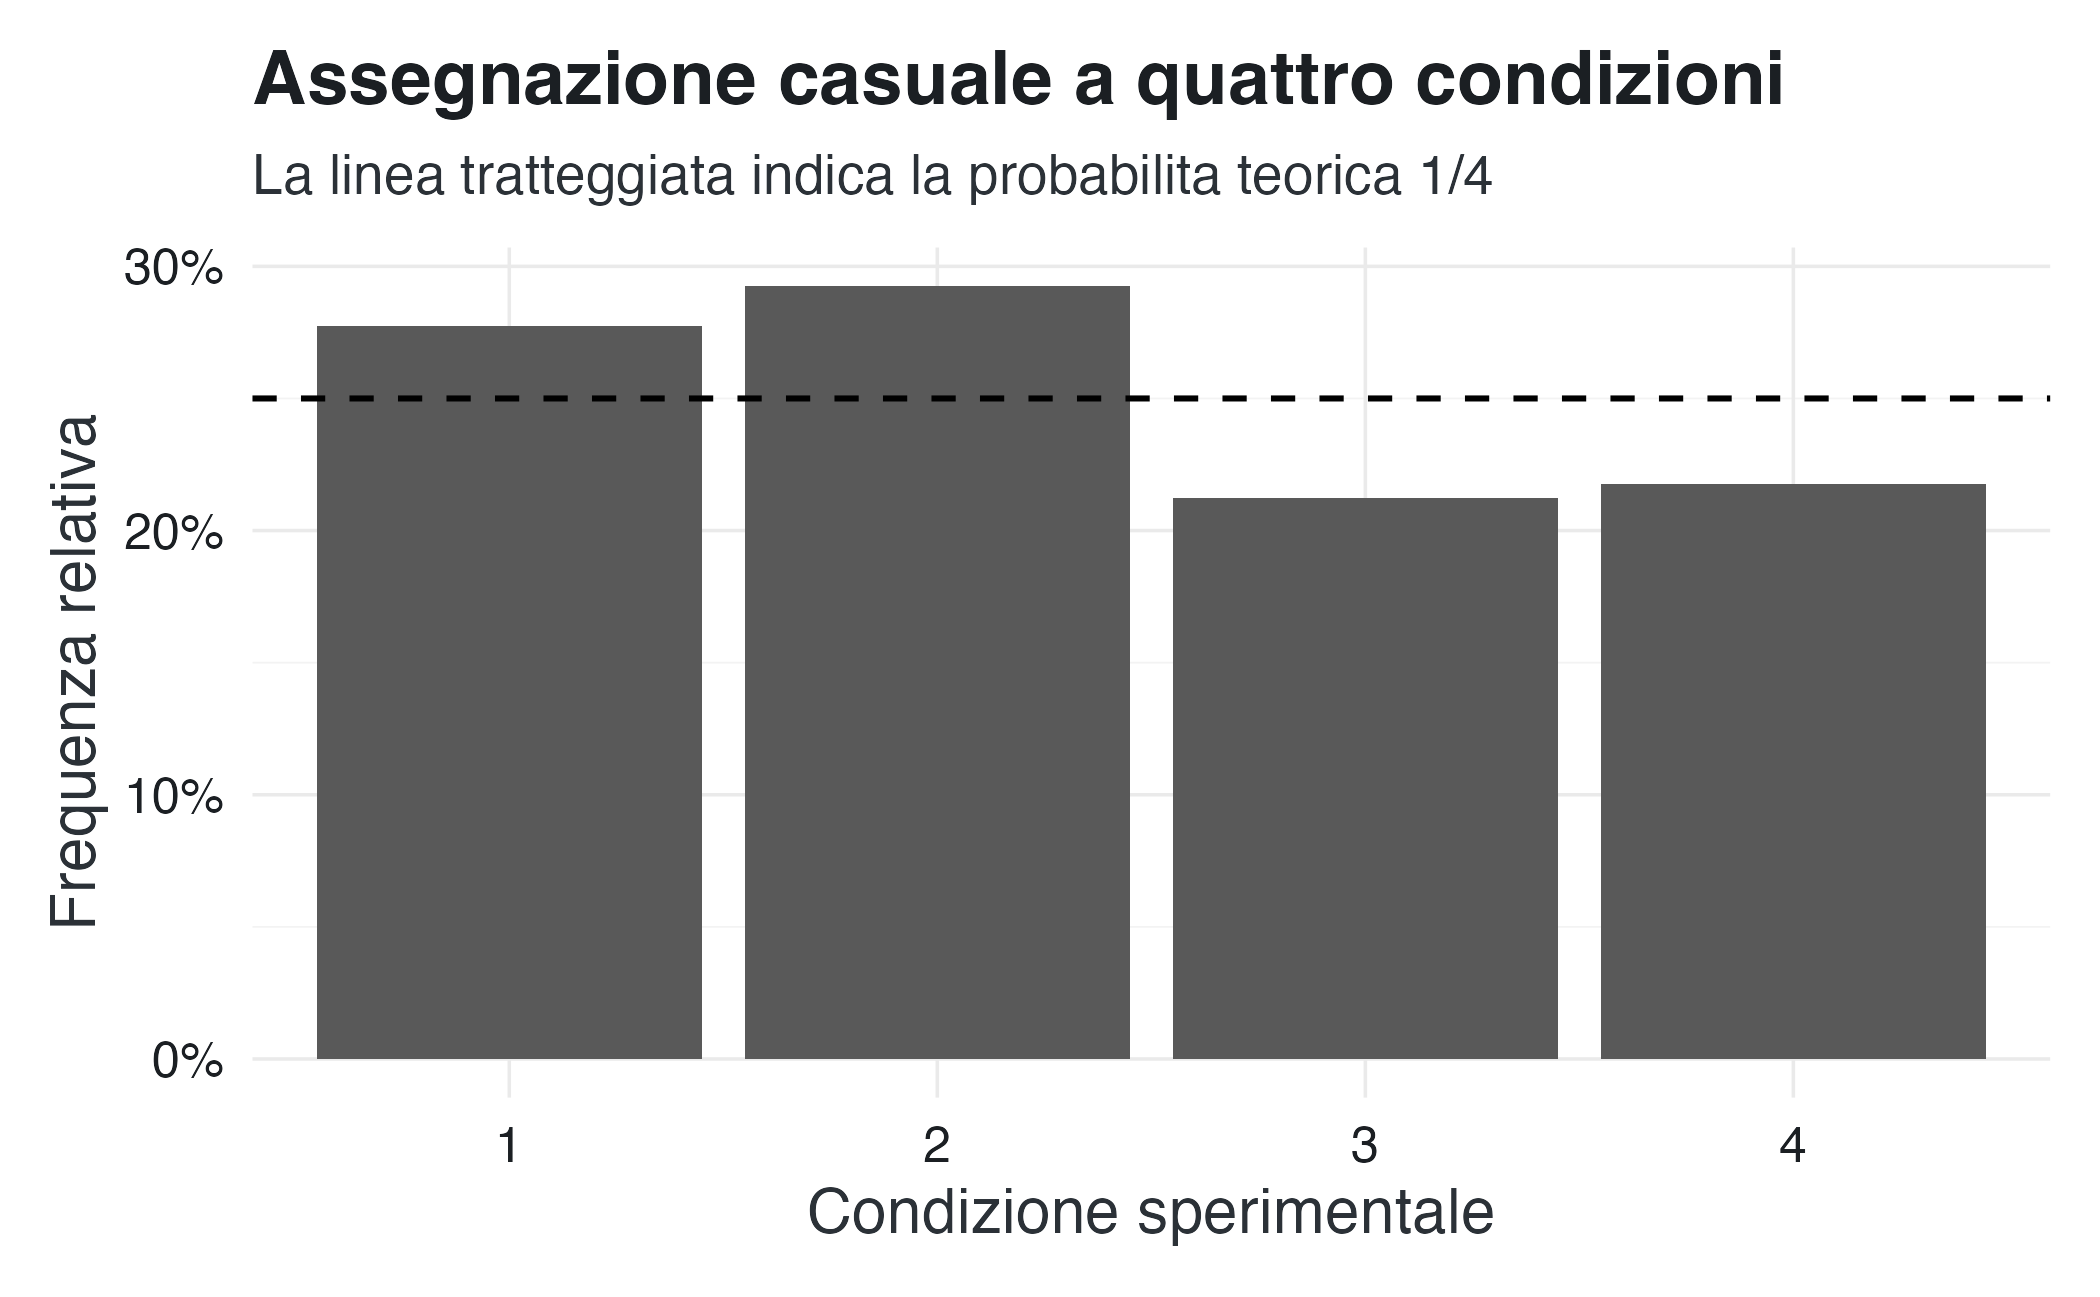
\includegraphics[width=0.85\linewidth,height=\textheight,keepaspectratio]{chapters/probability/11_discr_rv_distr_files/figure-pdf/unnamed-chunk-3-1.png}
\end{center}

\begin{tcolorbox}[enhanced jigsaw, arc=.35mm, bottomrule=.15mm, bottomtitle=1mm, breakable, colback=white, colbacktitle=quarto-callout-note-color!10!white, colframe=quarto-callout-note-color-frame, coltitle=black, left=2mm, leftrule=.75mm, opacityback=0, opacitybacktitle=0.6, rightrule=.15mm, title=\textcolor{quarto-callout-note-color}{\faInfo}\hspace{0.5em}{Interpretazione bayesiana}, titlerule=0mm, toprule=.15mm, toptitle=1mm]

Una distribuzione uniforme su un insieme finito puo anche rappresentare
una prior simmetrica su ipotesi o modelli alternativi:

\[
P(M_1)=P(M_2)=\cdots=P(M_K)=\frac{1}{K}.
\]

Questa scelta non significa che i modelli siano tutti ugualmente validi,
ma che prima di analizzare i dati non introduciamo alcuna preferenza tra
di essi.

\end{tcolorbox}

\section{Distribuzione di Bernoulli}\label{sec-bernoulli-distribution}

\subsection{Definizione}\label{definizione-1}

\begin{definition}[]\protect\hypertarget{def-bernoulli}{}\label{def-bernoulli}

Una variabile casuale \(X\) segue una distribuzione di Bernoulli se può
assumere solo due valori, convenzionalmente codificati come 1 e 0:

\[
X \sim \mathrm{Bernoulli}(p),
\qquad
P(X=x) = p^x(1-p)^{1-x},
\quad x \in \{0,1\}.
\]

I suoi momenti principali sono:

\[
\mathbb{E}(X) = p,
\qquad
\mathbb{V}(X) = p(1-p).
\]

\end{definition}

Il modello di Bernoulli è il più semplice per un dato binario. Il valore
1 non deve essere interpretato come un successo in senso stretto: è solo
l'esito che abbiamo scelto di codificare come tale. In psicologia può
indicare una risposta corretta, la presenza di un sintomo, l'adesione a
un trattamento o una scelta tra due alternative.

\subsection{Esempio: risposta corretta a un
item}\label{esempio-risposta-corretta-a-un-item}

Un partecipante risponde a un item di memoria. Se la probabilità di
risposta corretta è \(p = 0.70\), la risposta \(X\) può essere modellata
come:

\[
X \mid p = 0.70 \sim \mathrm{Bernoulli}(0.70).
\]

\begin{Shaded}
\begin{Highlighting}[]
\NormalTok{p }\OtherTok{\textless{}{-}} \FloatTok{0.70}
\NormalTok{bern\_df }\OtherTok{\textless{}{-}} \FunctionTok{data.frame}\NormalTok{(}
  \AttributeTok{esito =} \FunctionTok{factor}\NormalTok{(}\FunctionTok{c}\NormalTok{(}\DecValTok{0}\NormalTok{, }\DecValTok{1}\NormalTok{), }\AttributeTok{labels =} \FunctionTok{c}\NormalTok{(}\StringTok{"Errata"}\NormalTok{, }\StringTok{"Corretta"}\NormalTok{)),}
  \AttributeTok{probabilita =} \FunctionTok{c}\NormalTok{(}\DecValTok{1} \SpecialCharTok{{-}}\NormalTok{ p, p)}
\NormalTok{)}

\FunctionTok{ggplot}\NormalTok{(bern\_df, }\FunctionTok{aes}\NormalTok{(}\AttributeTok{x =}\NormalTok{ esito, }\AttributeTok{y =}\NormalTok{ probabilita)) }\SpecialCharTok{+}
  \FunctionTok{geom\_col}\NormalTok{() }\SpecialCharTok{+}
  \FunctionTok{scale\_y\_continuous}\NormalTok{(}\AttributeTok{labels =}\NormalTok{ scales}\SpecialCharTok{::}\FunctionTok{percent\_format}\NormalTok{()) }\SpecialCharTok{+}
  \FunctionTok{labs}\NormalTok{(}
    \AttributeTok{title =} \StringTok{"Distribuzione di Bernoulli"}\NormalTok{,}
    \AttributeTok{subtitle =} \StringTok{"Probabilita di risposta corretta p = 0.70"}\NormalTok{,}
    \AttributeTok{x =} \StringTok{"Esito"}\NormalTok{,}
    \AttributeTok{y =} \StringTok{"Probabilita"}
\NormalTok{  )}
\end{Highlighting}
\end{Shaded}

\begin{center}
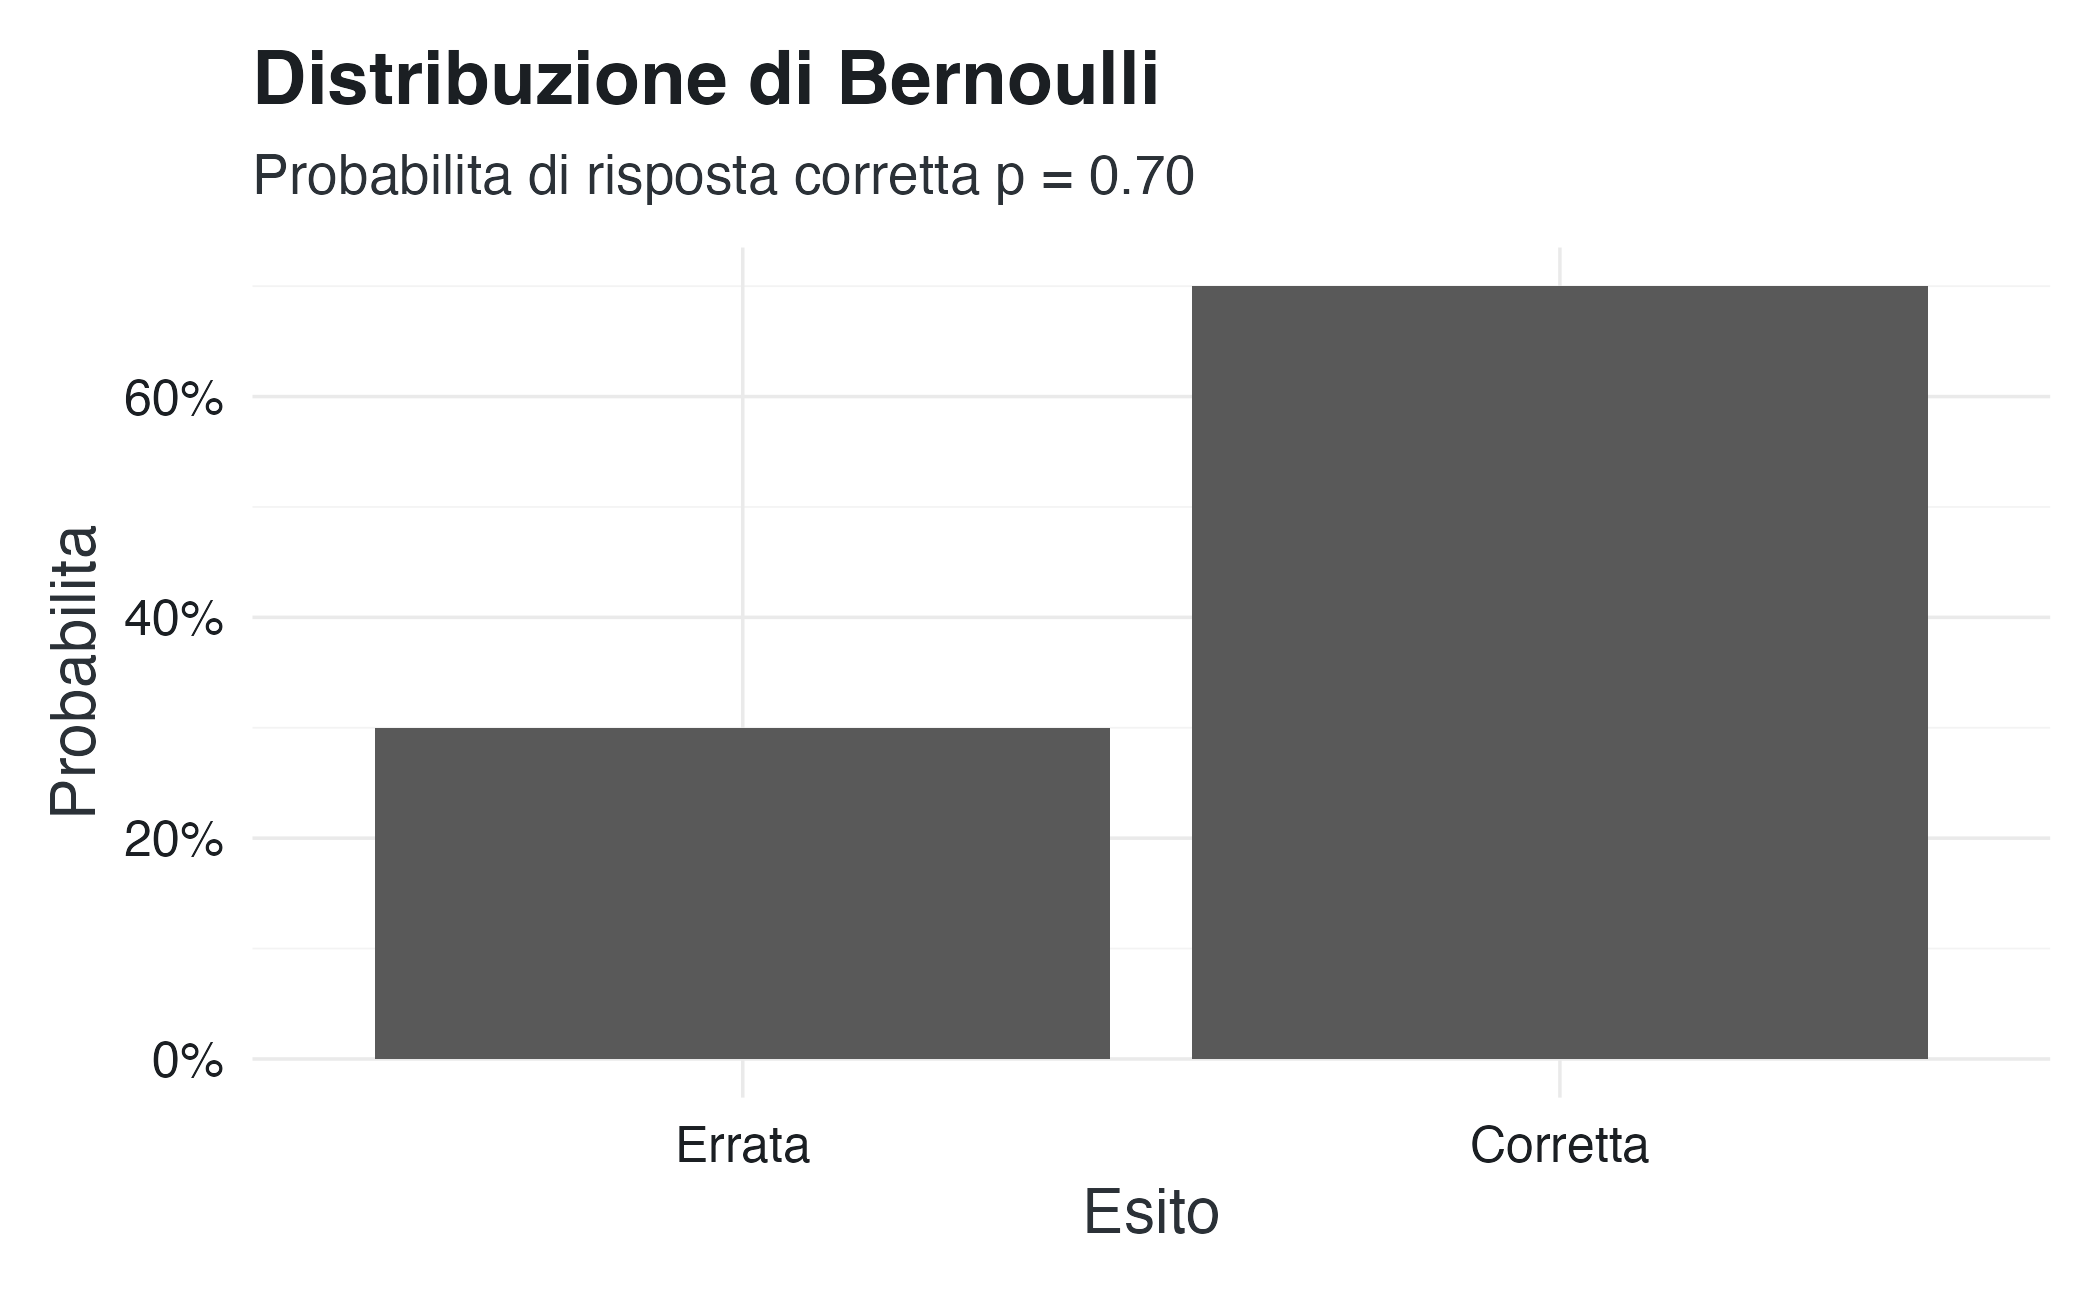
\includegraphics[width=0.85\linewidth,height=\textheight,keepaspectratio]{chapters/probability/11_discr_rv_distr_files/figure-pdf/unnamed-chunk-4-1.png}
\end{center}

\begin{Shaded}
\begin{Highlighting}[]
\FunctionTok{set.seed}\NormalTok{(}\DecValTok{123}\NormalTok{)}
\NormalTok{risposte }\OtherTok{\textless{}{-}} \FunctionTok{rbinom}\NormalTok{(}\DecValTok{20}\NormalTok{, }\AttributeTok{size =} \DecValTok{1}\NormalTok{, }\AttributeTok{prob =}\NormalTok{ p)}
\NormalTok{risposte}
\CommentTok{\#\textgreater{}  [1] 1 0 1 0 0 1 1 0 1 1 0 1 1 1 1 0 1 1 1 0}
\FunctionTok{mean}\NormalTok{(risposte)}
\CommentTok{\#\textgreater{} [1] 0.65}
\end{Highlighting}
\end{Shaded}

Anche se il parametro usato nella simulazione è \(p = 0.70\), in un
campione piccolo la proporzione osservata può discostarsi sensibilmente
da 0.70. Questo è il punto che verrà ripreso nel
Capitolo~\ref{sec-prob-inference-uncertainty}: i dati osservati sono
informativi, ma sono anche soggetti a variabilità campionaria.

\subsection{Bernoulli come modello
generativo}\label{bernoulli-come-modello-generativo}

Per una sequenza di risposte binarie \(X_1,\ldots,X_n\), spesso
assumiamo:

\[
X_i \mid p \sim \mathrm{Bernoulli}(p),
\qquad i=1,\ldots,n.
\]

Questa notazione indica che ogni osservazione è generata dallo stesso
meccanismo probabilistico. L'assunzione è semplice, ma forte: implica
che le osservazioni siano indipendenti e che la probabilità di ottenere
un esito 1 sia la stessa per tutte le osservazioni.

\begin{tcolorbox}[enhanced jigsaw, arc=.35mm, bottomrule=.15mm, bottomtitle=1mm, breakable, colback=white, colbacktitle=quarto-callout-warning-color!10!white, colframe=quarto-callout-warning-color-frame, coltitle=black, left=2mm, leftrule=.75mm, opacityback=0, opacitybacktitle=0.6, rightrule=.15mm, title=\textcolor{quarto-callout-warning-color}{\faExclamationTriangle}\hspace{0.5em}{Quando la Bernoulli e troppo semplice}, titlerule=0mm, toprule=.15mm, toptitle=1mm]

Nei dati psicologici reali, l'assunzione di un unico valore di \(p\) può
essere irrealistica. Ad esempio, gli item diversi possono avere
difficoltà diverse, i partecipanti possono avere abilità diverse, e le
risposte successive possono non essere indipendenti.

La distribuzione di Bernoulli rimane comunque il punto di partenza: i
modelli più ricchi spesso nascono proprio dal rilassamento di una o più
delle sue assunzioni.

\end{tcolorbox}

\section{Distribuzione binomiale}\label{sec-binomial-distribution}

\subsection{Dalla Bernoulli alla
binomiale}\label{dalla-bernoulli-alla-binomiale}

La distribuzione binomiale descrive il numero di successi in \(n\) prove
di Bernoulli indipendenti, tutte con la stessa probabilità di successo
\(p\).

Se

\[
X_1,\ldots,X_n \mid p \sim \mathrm{Bernoulli}(p),
\] e definiamo

\[
Y = \sum_{i=1}^n X_i,
\] allora \(Y\) rappresenta il numero totale di successi. In questo
caso:

\[
Y \mid p \sim \mathrm{Binomiale}(n,p).
\]

\subsection{Perche compare il coefficiente
binomiale?}\label{perche-compare-il-coefficiente-binomiale}

Se osserviamo esattamente \(k\) successi e \(n-k\) insuccessi, la
probabilità di una sequenza specifica è:

\[
p^k(1-p)^{n-k}.
\]

Tuttavia, lo stesso numero di successi può comparire in molti ordini
diversi. Il numero di sequenze con \(k\) successi in \(n\) prove è:

\[
\binom{n}{k}.
\] Quindi, la probabilità complessiva di osservare \(k\) successi è:

\[
P(Y=k \mid p,n) = \binom{n}{k}p^k(1-p)^{n-k}.
\]

\subsection{Definizione}\label{definizione-2}

\begin{definition}[]\protect\hypertarget{def-binomial}{}\label{def-binomial}

Una variabile casuale \(Y\) segue una distribuzione binomiale con
parametri \(n\) e \(p\) se:

\[
Y \sim \mathrm{Binomiale}(n,p),
\qquad
P(Y=k)=\binom{n}{k}p^k(1-p)^{n-k},
\quad k=0,1,\ldots,n.
\]

I suoi momenti principali sono:

\[
\mathbb{E}(Y)=np,
\qquad
\mathbb{V}(Y)=np(1-p).
\]

\end{definition}

\subsection{Esempio: punteggio a un
test}\label{esempio-punteggio-a-un-test}

Un test contiene 20 item dicotomici. Se la probabilità di risposta
corretta a ciascun item è \(p=0.75\), il numero totale di risposte
corrette può essere modellato come:

\[
Y \mid p=0.75 \sim \mathrm{Binomiale}(20,0.75).
\]

\begin{Shaded}
\begin{Highlighting}[]
\NormalTok{n\_item }\OtherTok{\textless{}{-}} \DecValTok{20}
\NormalTok{p\_corretto }\OtherTok{\textless{}{-}} \FloatTok{0.75}
\NormalTok{k }\OtherTok{\textless{}{-}} \DecValTok{0}\SpecialCharTok{:}\NormalTok{n\_item}

\NormalTok{binom\_df }\OtherTok{\textless{}{-}} \FunctionTok{data.frame}\NormalTok{(}
  \AttributeTok{k =}\NormalTok{ k,}
  \AttributeTok{probabilita =} \FunctionTok{dbinom}\NormalTok{(k, }\AttributeTok{size =}\NormalTok{ n\_item, }\AttributeTok{prob =}\NormalTok{ p\_corretto)}
\NormalTok{)}

\FunctionTok{ggplot}\NormalTok{(binom\_df, }\FunctionTok{aes}\NormalTok{(}\AttributeTok{x =}\NormalTok{ k, }\AttributeTok{y =}\NormalTok{ probabilita)) }\SpecialCharTok{+}
  \FunctionTok{geom\_col}\NormalTok{() }\SpecialCharTok{+}
  \FunctionTok{scale\_x\_continuous}\NormalTok{(}\AttributeTok{breaks =} \DecValTok{0}\SpecialCharTok{:}\NormalTok{n\_item) }\SpecialCharTok{+}
  \FunctionTok{labs}\NormalTok{(}
    \AttributeTok{title =} \StringTok{"Distribuzione binomiale"}\NormalTok{,}
    \AttributeTok{subtitle =} \StringTok{"Numero di risposte corrette su 20 item, p = 0.75"}\NormalTok{,}
    \AttributeTok{x =} \StringTok{"Risposte corrette"}\NormalTok{,}
    \AttributeTok{y =} \StringTok{"Probabilita"}
\NormalTok{  )}
\end{Highlighting}
\end{Shaded}

\begin{center}
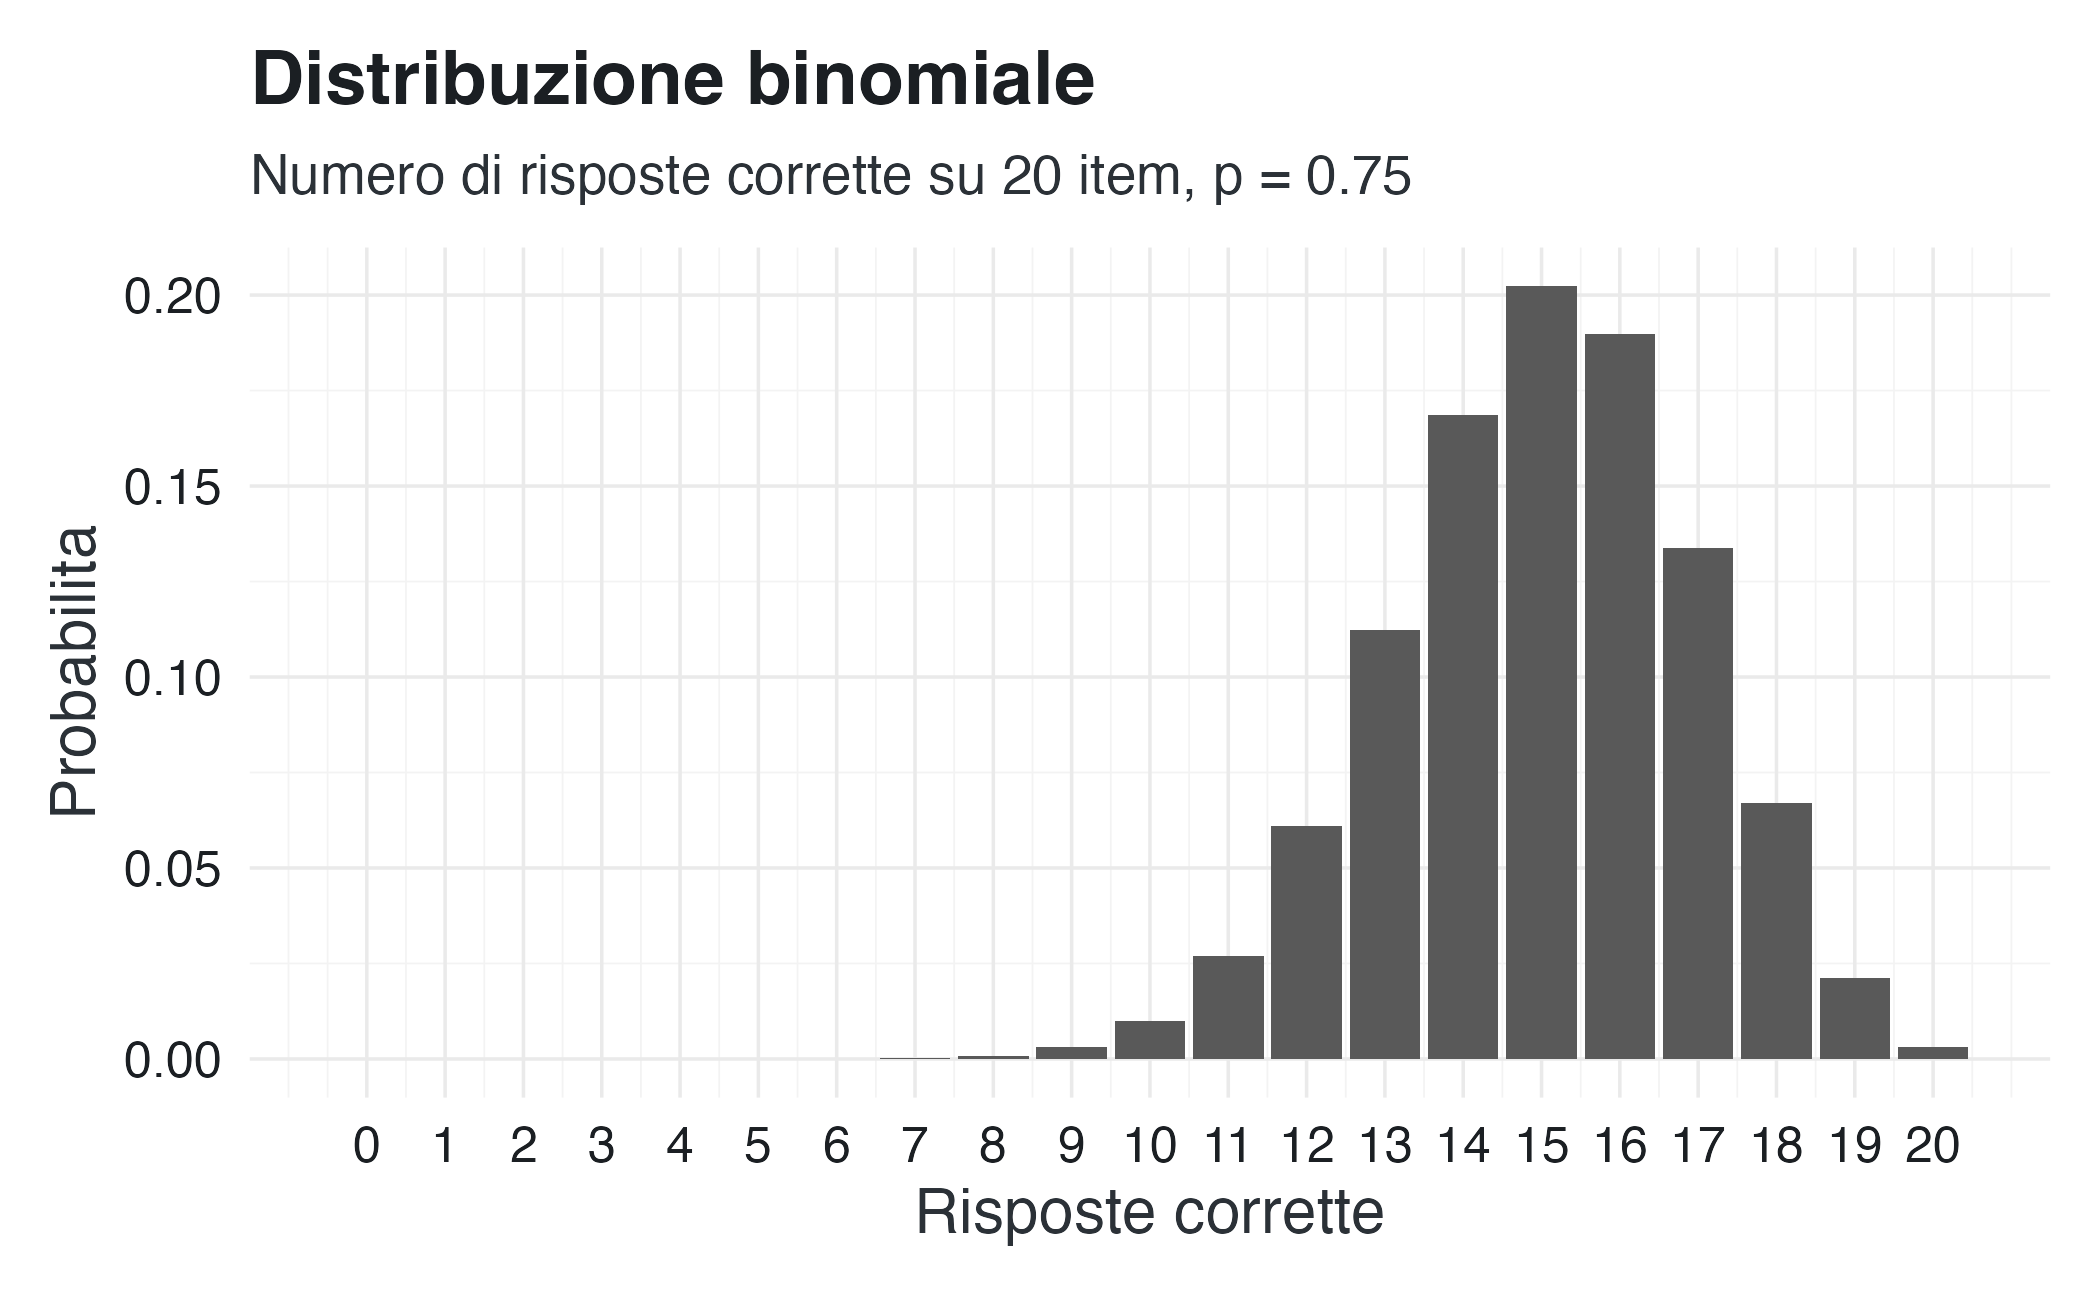
\includegraphics[width=0.85\linewidth,height=\textheight,keepaspectratio]{chapters/probability/11_discr_rv_distr_files/figure-pdf/unnamed-chunk-6-1.png}
\end{center}

\begin{Shaded}
\begin{Highlighting}[]
\NormalTok{media\_teorica }\OtherTok{\textless{}{-}}\NormalTok{ n\_item }\SpecialCharTok{*}\NormalTok{ p\_corretto}
\NormalTok{var\_teorica }\OtherTok{\textless{}{-}}\NormalTok{ n\_item }\SpecialCharTok{*}\NormalTok{ p\_corretto }\SpecialCharTok{*}\NormalTok{ (}\DecValTok{1} \SpecialCharTok{{-}}\NormalTok{ p\_corretto)}

\FunctionTok{cat}\NormalTok{(}\StringTok{"Media teorica:"}\NormalTok{, media\_teorica, }\StringTok{"}\SpecialCharTok{\textbackslash{}n}\StringTok{"}\NormalTok{)}
\CommentTok{\#\textgreater{} Media teorica: 15}
\FunctionTok{cat}\NormalTok{(}\StringTok{"Varianza teorica:"}\NormalTok{, var\_teorica, }\StringTok{"}\SpecialCharTok{\textbackslash{}n}\StringTok{"}\NormalTok{)}
\CommentTok{\#\textgreater{} Varianza teorica: 3.75}
\end{Highlighting}
\end{Shaded}

\subsection{La proporzione
campionaria}\label{la-proporzione-campionaria}

Spesso non ci interessa solo il numero totale di successi \(Y\), ma
anche la proporzione:

\[
\hat p = \frac{Y}{n}.
\]

Poiché \(Y \sim \mathrm{Binomiale}(n,p)\), otteniamo:

\[
\mathbb{E}(\hat p)=p,
\qquad
\mathbb{V}(\hat p)=\frac{p(1-p)}{n}.
\]

Questa relazione sarà centrale nel
Capitolo~\ref{sec-prob-inference-uncertainty}: mostra perché campioni
più grandi producono proporzioni più stabili.

\begin{Shaded}
\begin{Highlighting}[]
\FunctionTok{set.seed}\NormalTok{(}\DecValTok{42}\NormalTok{)}
\NormalTok{n\_values }\OtherTok{\textless{}{-}} \FunctionTok{c}\NormalTok{(}\DecValTok{10}\NormalTok{, }\DecValTok{50}\NormalTok{, }\DecValTok{200}\NormalTok{)}
\NormalTok{p\_vero }\OtherTok{\textless{}{-}} \FloatTok{0.40}
\NormalTok{n\_rep }\OtherTok{\textless{}{-}} \DecValTok{5000}

\NormalTok{sim\_list }\OtherTok{\textless{}{-}} \FunctionTok{lapply}\NormalTok{(n\_values, }\ControlFlowTok{function}\NormalTok{(n) \{}
\NormalTok{  phat }\OtherTok{\textless{}{-}} \FunctionTok{rbinom}\NormalTok{(n\_rep, }\AttributeTok{size =}\NormalTok{ n, }\AttributeTok{prob =}\NormalTok{ p\_vero) }\SpecialCharTok{/}\NormalTok{ n}
  \FunctionTok{data.frame}\NormalTok{(}\AttributeTok{n =} \FunctionTok{factor}\NormalTok{(n), }\AttributeTok{phat =}\NormalTok{ phat)}
\NormalTok{\})}

\NormalTok{sim\_df }\OtherTok{\textless{}{-}} \FunctionTok{do.call}\NormalTok{(rbind, sim\_list)}

\FunctionTok{ggplot}\NormalTok{(sim\_df, }\FunctionTok{aes}\NormalTok{(}\AttributeTok{x =}\NormalTok{ phat)) }\SpecialCharTok{+}
  \FunctionTok{geom\_histogram}\NormalTok{(}\AttributeTok{bins =} \DecValTok{30}\NormalTok{) }\SpecialCharTok{+}
  \FunctionTok{facet\_wrap}\NormalTok{(}\SpecialCharTok{\textasciitilde{}}\NormalTok{ n, }\AttributeTok{ncol =} \DecValTok{1}\NormalTok{) }\SpecialCharTok{+}
  \FunctionTok{labs}\NormalTok{(}
    \AttributeTok{title =} \StringTok{"Distribuzione simulata della proporzione campionaria"}\NormalTok{,}
    \AttributeTok{subtitle =} \StringTok{"La variabilita diminuisce al crescere di n"}\NormalTok{,}
    \AttributeTok{x =} \StringTok{"Proporzione osservata"}\NormalTok{,}
    \AttributeTok{y =} \StringTok{"Frequenza"}
\NormalTok{  )}
\end{Highlighting}
\end{Shaded}

\begin{center}
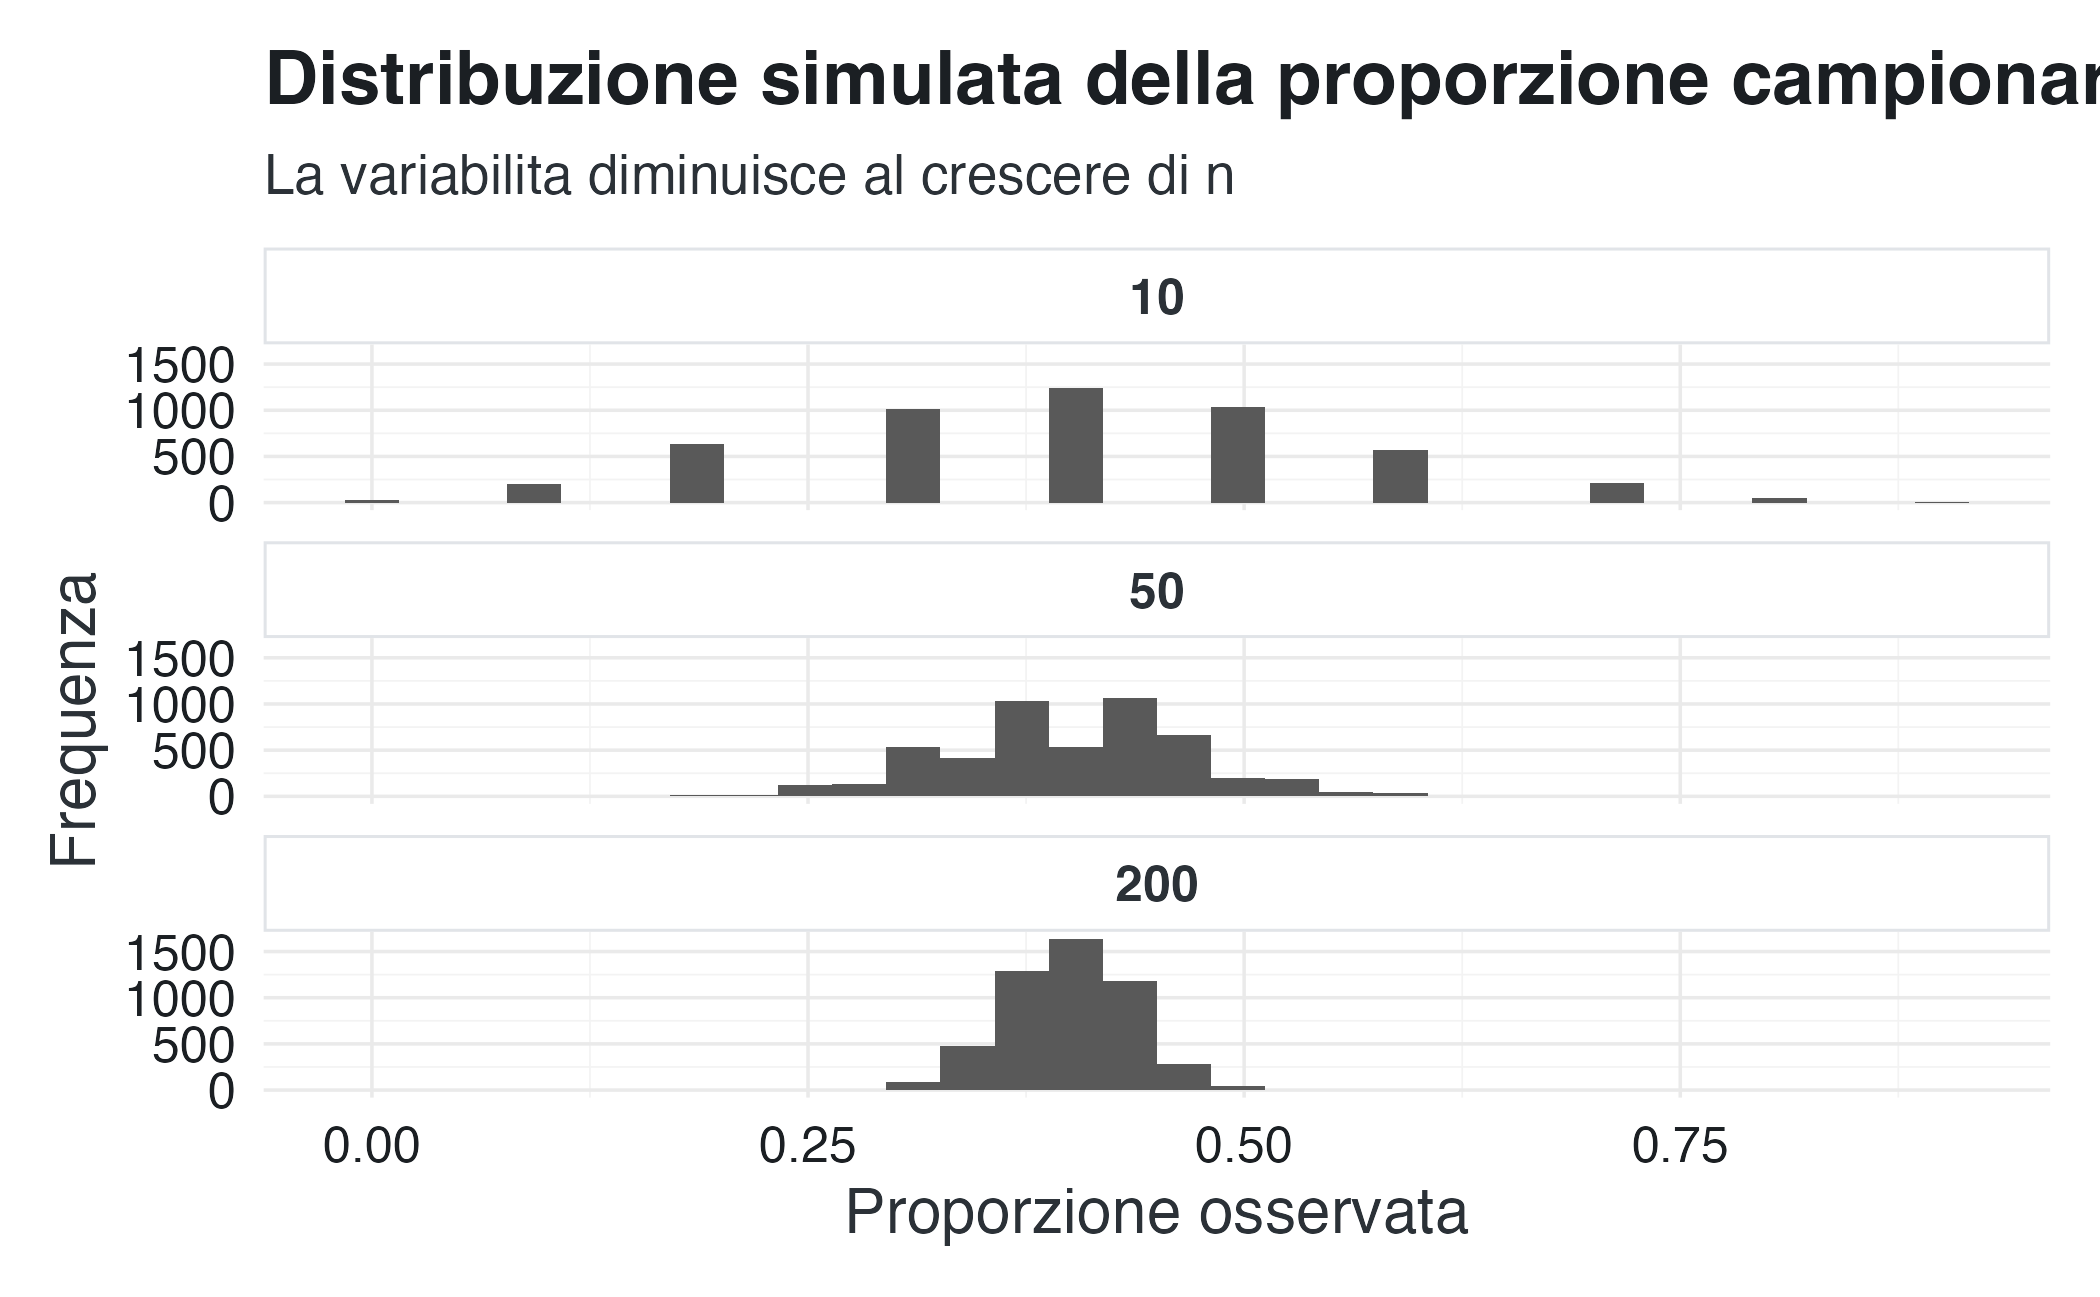
\includegraphics[width=0.85\linewidth,height=\textheight,keepaspectratio]{chapters/probability/11_discr_rv_distr_files/figure-pdf/unnamed-chunk-8-1.png}
\end{center}

\subsection{Ruolo bayesiano: la binomiale come
verosimiglianza}\label{ruolo-bayesiano-la-binomiale-come-verosimiglianza}

Se osserviamo \(y\) successi su \(n\) prove, la distribuzione binomiale
può essere riletta come funzione di \(p\):

\[
L(p \mid y,n) \propto p^y(1-p)^{n-y}.
\]

Questa espressione non è ancora una distribuzione a posteriori. È la
\textbf{verosimiglianza}: descrive quanto i dati osservati siano
compatibili con ciascun valore possibile di \(p\).

\begin{tcolorbox}[enhanced jigsaw, arc=.35mm, bottomrule=.15mm, bottomtitle=1mm, breakable, colback=white, colbacktitle=quarto-callout-note-color!10!white, colframe=quarto-callout-note-color-frame, coltitle=black, left=2mm, leftrule=.75mm, opacityback=0, opacitybacktitle=0.6, rightrule=.15mm, title=\textcolor{quarto-callout-note-color}{\faInfo}\hspace{0.5em}{Anticipazione: prior Beta e aggiornamento}, titlerule=0mm, toprule=.15mm, toptitle=1mm]

Nei capitoli successivi introdurremo la distribuzione Beta, una
distribuzione continua su \([0,1]\) molto utile per rappresentare
l'incertezza su una probabilità \(p\).

Se

\[
p \sim \mathrm{Beta}(\alpha,\beta)
\] e osserviamo \(y\) successi su \(n\) prove, allora la posterior è:

\[
p \mid y,n \sim \mathrm{Beta}(\alpha+y,\beta+n-y).
\]

Per ora non è necessario padroneggiare questa formula. È sufficiente
riconoscere che i dati binomiali aggiornano le credenze su una
probabilità.

\end{tcolorbox}

\section{Distribuzione di Poisson}\label{sec-poisson-distribution}

\subsection{Quando usarla}\label{quando-usarla}

La distribuzione di Poisson descrive il numero di eventi in un
intervallo di tempo, spazio o esposizione. È valida quando:

\begin{itemize}
\tightlist
\item
  gli eventi sono conteggiabili;
\item
  l'intervallo di osservazione è ben definito;
\item
  il tasso medio di occorrenza è pressoché costante;
\item
  gli eventi sono tra loro approssimativamente indipendenti;
\item
  la coincidenza di due eventi è improbabile, specie per intervalli
  brevi.
\end{itemize}

In psicologia, esempi comuni sono:

\begin{itemize}
\tightlist
\item
  attacchi di panico in un mese;
\item
  errori di omissione in un compito attentivo;
\item
  risvegli notturni;
\item
  comportamenti target osservati in una sessione.
\end{itemize}

\subsection{Definizione}\label{definizione-3}

\begin{definition}[]\protect\hypertarget{def-poisson}{}\label{def-poisson}

Una variabile casuale \(Y\) segue una distribuzione di Poisson con
parametro \(\lambda > 0\) se:

\[
Y \sim \mathrm{Poisson}(\lambda),
\qquad
P(Y=y)=\frac{\lambda^y e^{-\lambda}}{y!},
\quad y=0,1,2,\ldots.
\]

La sua proprieta caratteristica è:

\[
\mathbb{E}(Y)=\mathbb{V}(Y)=\lambda.
\]

\end{definition}

Il parametro \(\lambda\) rappresenta il numero medio atteso di eventi
nell'intervallo considerato. Se \(\lambda=2.5\), ci aspettiamo in media
2.5 eventi per intervallo, ma il numero osservato potra essere 0, 1, 2,
3, e così via.

\begin{Shaded}
\begin{Highlighting}[]
\NormalTok{lambda }\OtherTok{\textless{}{-}} \FloatTok{2.5}
\NormalTok{y }\OtherTok{\textless{}{-}} \DecValTok{0}\SpecialCharTok{:}\DecValTok{12}
\NormalTok{pois\_df }\OtherTok{\textless{}{-}} \FunctionTok{data.frame}\NormalTok{(}
  \AttributeTok{y =}\NormalTok{ y,}
  \AttributeTok{probabilita =} \FunctionTok{dpois}\NormalTok{(y, }\AttributeTok{lambda =}\NormalTok{ lambda)}
\NormalTok{)}

\FunctionTok{ggplot}\NormalTok{(pois\_df, }\FunctionTok{aes}\NormalTok{(}\AttributeTok{x =}\NormalTok{ y, }\AttributeTok{y =}\NormalTok{ probabilita)) }\SpecialCharTok{+}
  \FunctionTok{geom\_col}\NormalTok{() }\SpecialCharTok{+}
  \FunctionTok{scale\_x\_continuous}\NormalTok{(}\AttributeTok{breaks =}\NormalTok{ y) }\SpecialCharTok{+}
  \FunctionTok{labs}\NormalTok{(}
    \AttributeTok{title =} \StringTok{"Distribuzione di Poisson"}\NormalTok{,}
    \AttributeTok{subtitle =} \StringTok{"Conteggi attesi con lambda = 2.5"}\NormalTok{,}
    \AttributeTok{x =} \StringTok{"Numero di eventi"}\NormalTok{,}
    \AttributeTok{y =} \StringTok{"Probabilita"}
\NormalTok{  )}
\end{Highlighting}
\end{Shaded}

\begin{center}
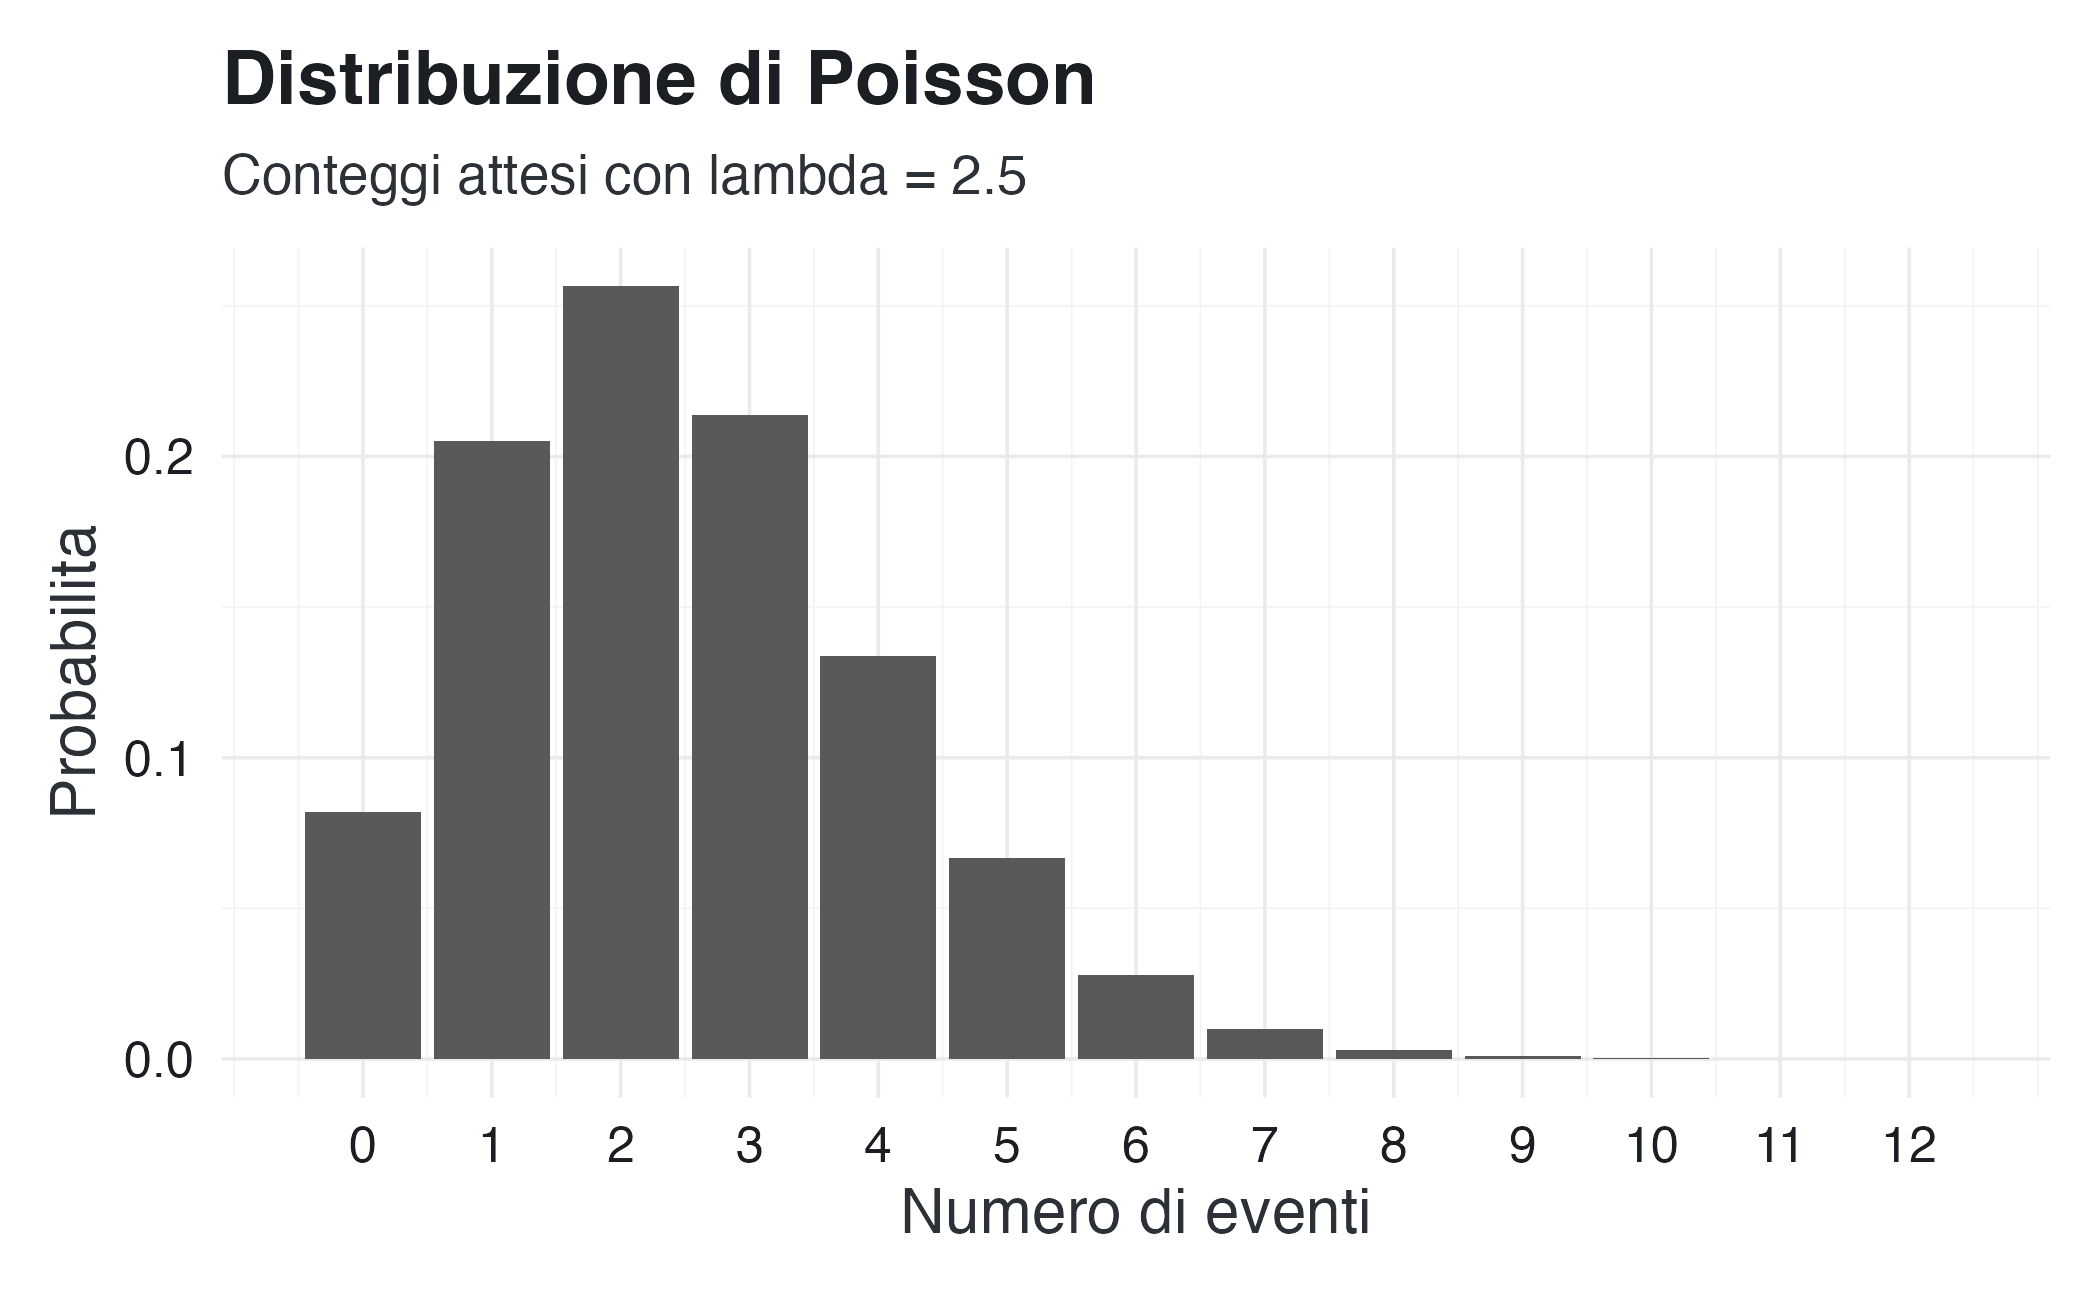
\includegraphics[width=0.85\linewidth,height=\textheight,keepaspectratio]{chapters/probability/11_discr_rv_distr_files/figure-pdf/unnamed-chunk-9-1.png}
\end{center}

\subsection{Esempio clinico}\label{esempio-clinico}

Un clinico sta monitorando il numero di attacchi di panico riportati da
un paziente in un mese. Se il tasso medio atteso è \(\lambda = 2.5\)
attacchi al mese, allora:

\[
Y \mid \lambda = 2.5 \sim \mathrm{Poisson}(2.5).
\]

\begin{Shaded}
\begin{Highlighting}[]
\FunctionTok{set.seed}\NormalTok{(}\DecValTok{123}\NormalTok{)}
\NormalTok{mesi }\OtherTok{\textless{}{-}} \DecValTok{24}
\NormalTok{attacchi }\OtherTok{\textless{}{-}} \FunctionTok{rpois}\NormalTok{(mesi, }\AttributeTok{lambda =} \FloatTok{2.5}\NormalTok{)}

\FunctionTok{data.frame}\NormalTok{(}
  \AttributeTok{mese =} \DecValTok{1}\SpecialCharTok{:}\NormalTok{mesi,}
  \AttributeTok{attacchi =}\NormalTok{ attacchi}
\NormalTok{)}
\CommentTok{\#\textgreater{}    mese attacchi}
\CommentTok{\#\textgreater{} 1     1        2}
\CommentTok{\#\textgreater{} 2     2        4}
\CommentTok{\#\textgreater{} 3     3        2}
\CommentTok{\#\textgreater{} 4     4        4}
\CommentTok{\#\textgreater{} 5     5        5}
\CommentTok{\#\textgreater{} 6     6        0}
\CommentTok{\#\textgreater{} 7     7        2}
\CommentTok{\#\textgreater{} 8     8        5}
\CommentTok{\#\textgreater{} 9     9        3}
\CommentTok{\#\textgreater{} 10   10        2}
\CommentTok{\#\textgreater{} 11   11        5}
\CommentTok{\#\textgreater{} 12   12        2}
\CommentTok{\#\textgreater{} 13   13        3}
\CommentTok{\#\textgreater{} 14   14        3}
\CommentTok{\#\textgreater{} 15   15        1}
\CommentTok{\#\textgreater{} 16   16        5}
\CommentTok{\#\textgreater{} 17   17        1}
\CommentTok{\#\textgreater{} 18   18        0}
\CommentTok{\#\textgreater{} 19   19        2}
\CommentTok{\#\textgreater{} 20   20        5}
\CommentTok{\#\textgreater{} 21   21        4}
\CommentTok{\#\textgreater{} 22   22        3}
\CommentTok{\#\textgreater{} 23   23        3}
\CommentTok{\#\textgreater{} 24   24        7}
\end{Highlighting}
\end{Shaded}

\begin{Shaded}
\begin{Highlighting}[]
\FunctionTok{cat}\NormalTok{(}\StringTok{"Media osservata:"}\NormalTok{, }\FunctionTok{round}\NormalTok{(}\FunctionTok{mean}\NormalTok{(attacchi), }\DecValTok{2}\NormalTok{), }\StringTok{"}\SpecialCharTok{\textbackslash{}n}\StringTok{"}\NormalTok{)}
\CommentTok{\#\textgreater{} Media osservata: 3.04}
\FunctionTok{cat}\NormalTok{(}\StringTok{"Varianza osservata:"}\NormalTok{, }\FunctionTok{round}\NormalTok{(}\FunctionTok{var}\NormalTok{(attacchi), }\DecValTok{2}\NormalTok{), }\StringTok{"}\SpecialCharTok{\textbackslash{}n}\StringTok{"}\NormalTok{)}
\CommentTok{\#\textgreater{} Varianza osservata: 3.09}
\end{Highlighting}
\end{Shaded}

Con pochi mesi di osservazione, media e varianza empiriche possono
differire. Tuttavia, se la Poisson è un modello adeguato, su campioni
grandi ci aspettiamo che media e varianza siano simili.

\subsection{Tassi ed esposizione}\label{tassi-ed-esposizione}

Spesso gli intervalli di osservazione non hanno la stessa durata. In
questo caso non e sufficiente confrontare i conteggi grezzi: ma bisogna
tenere conto dell'\textbf{esposizione}.

Se \(t_i\) è la durata dell'osservazione per l'unità \(i\), possiamo
scrivere:

\[
Y_i \mid \lambda,t_i \sim \mathrm{Poisson}(\lambda t_i),
\] dove \(\lambda\) è il tasso per unità di esposizione.

\begin{tcolorbox}[enhanced jigsaw, arc=.35mm, bottomrule=.15mm, bottomtitle=1mm, breakable, colback=white, colbacktitle=quarto-callout-note-color!10!white, colframe=quarto-callout-note-color-frame, coltitle=black, left=2mm, leftrule=.75mm, opacityback=0, opacitybacktitle=0.6, rightrule=.15mm, title=\textcolor{quarto-callout-note-color}{\faInfo}\hspace{0.5em}{Esempio}, titlerule=0mm, toprule=.15mm, toptitle=1mm]

Osservare 4 comportamenti problema in 2 ore non ha lo stesso significato
di osservarli in 20 minuti. Il conteggio è lo stesso, ma il tasso è
diverso.

\end{tcolorbox}

\subsection{Ruolo bayesiano: prior Gamma per un
tasso}\label{ruolo-bayesiano-prior-gamma-per-un-tasso}

Nel framework bayesiano, \(\lambda\) è una quantità incerta. Una scelta
frequente per rappresentare credenze su un tasso positivo e la
distribuzione Gamma, che verrà introdotta nel capitolo sulle
distribuzioni continue.

Se

\[
\lambda \sim \mathrm{Gamma}(\alpha,\beta),
\] e osserviamo conteggi indipendenti \(y_1,\ldots,y_n\) su intervalli
di uguale esposizione, allora:

\[
\lambda \mid \mathbf{y}
\sim
\mathrm{Gamma}\left(\alpha + \sum_{i=1}^n y_i,\; \beta+n\right),
\]

nella parametrizzazione in cui \(\beta\) e il tasso della Gamma.

Per ora, il punto fondamentale è il seguente: la distribuzione di
Poisson fornisce il modello dei conteggi, mentre la distribuzione di
Gamma rappresenta l'incertezza sul tasso che genera tali conteggi.

\section{Quando i modelli discreti semplici non
bastano}\label{sec-discrete-model-checks}

Le distribuzioni introdotte finora sono utili perché semplici e
interpretabili. Proprio per questo, però, incorporano assunzioni forti.

\subsection{Binomiale: indipendenza e probabilita
costante}\label{binomiale-indipendenza-e-probabilita-costante}

La distribuzione binomiale presuppone che tutte le prove abbiano la
stessa probabilità \(p\) e siano indipendenti. Questa assunzione può
essere problematica quando:

\begin{itemize}
\tightlist
\item
  gli item hanno difficoltà diverse;
\item
  i partecipanti sono molto differsi tra loro;
\item
  le prove successive sono influenzate dall'apprendimento, dala fatica o
  dalla memoria;
\item
  i dati provengono da gruppi o contesti differenti.
\end{itemize}

In questi casi, la variabilità osservata può essere maggiore di quella
prevista dalla distribuzione binomiale. In questo caso si parla di
\textbf{sovradispersione}.

\subsection{Poisson: equidispersione}\label{poisson-equidispersione}

La distribuzione di Poisson assume che media e varianza coincidano:

\[
\mathbb{E}(Y)=\mathbb{V}(Y)=\lambda.
\]

Nei dati psicologici, questa proprietà è spesso violata. Se la varianza
è molto maggiore della media, una distribuzione di Poisson semplice può
sottostimare l'incertezza.

\begin{Shaded}
\begin{Highlighting}[]
\CommentTok{\# Piccolo controllo descrittivo per dati di conteggio}
\NormalTok{media\_attacchi }\OtherTok{\textless{}{-}} \FunctionTok{mean}\NormalTok{(attacchi)}
\NormalTok{var\_attacchi }\OtherTok{\textless{}{-}} \FunctionTok{var}\NormalTok{(attacchi)}
\NormalTok{rapporto\_dispersione }\OtherTok{\textless{}{-}}\NormalTok{ var\_attacchi }\SpecialCharTok{/}\NormalTok{ media\_attacchi}

\FunctionTok{cat}\NormalTok{(}\StringTok{"Media:"}\NormalTok{, }\FunctionTok{round}\NormalTok{(media\_attacchi, }\DecValTok{2}\NormalTok{), }\StringTok{"}\SpecialCharTok{\textbackslash{}n}\StringTok{"}\NormalTok{)}
\CommentTok{\#\textgreater{} Media: 3.04}
\FunctionTok{cat}\NormalTok{(}\StringTok{"Varianza:"}\NormalTok{, }\FunctionTok{round}\NormalTok{(var\_attacchi, }\DecValTok{2}\NormalTok{), }\StringTok{"}\SpecialCharTok{\textbackslash{}n}\StringTok{"}\NormalTok{)}
\CommentTok{\#\textgreater{} Varianza: 3.09}
\FunctionTok{cat}\NormalTok{(}\StringTok{"Varianza / media:"}\NormalTok{, }\FunctionTok{round}\NormalTok{(rapporto\_dispersione, }\DecValTok{2}\NormalTok{), }\StringTok{"}\SpecialCharTok{\textbackslash{}n}\StringTok{"}\NormalTok{)}
\CommentTok{\#\textgreater{} Varianza / media: 1.01}
\end{Highlighting}
\end{Shaded}

\begin{tcolorbox}[enhanced jigsaw, arc=.35mm, bottomrule=.15mm, bottomtitle=1mm, breakable, colback=white, colbacktitle=quarto-callout-warning-color!10!white, colframe=quarto-callout-warning-color-frame, coltitle=black, left=2mm, leftrule=.75mm, opacityback=0, opacitybacktitle=0.6, rightrule=.15mm, title=\textcolor{quarto-callout-warning-color}{\faExclamationTriangle}\hspace{0.5em}{Il modello non e il fenomeno}, titlerule=0mm, toprule=.15mm, toptitle=1mm]

Una distribuzione discreta è una rappresentazione semplificata del
processo che potrebbe aver generato i dati. Non basta scegliere una
distribuzione perché il dominio sembra corretto: bisogna chiedersi se le
assunzioni del modello siano plausibili per il disegno di ricerca e per
il fenomeno psicologico studiato.

\end{tcolorbox}

\subsection{Anticipazione: distribuzioni predittive e
sovradispersione}\label{anticipazione-distribuzioni-predittive-e-sovradispersione}

Quando introduciamo l'incertezza sui parametri, le distribuzioni
predittive diventano più disperse rispetto ai modelli condizionali
semplici.

Ad esempio, se \(Y \mid p \sim \mathrm{Binomiale}(n,p)\) ma \(p\) non è
noto e viene modellato con una distribuzione Beta, la distribuzione
predittiva di \(Y\) diventa una \textbf{beta-binomiale}. Questa
distribuzione tiene conto sia della variabilità campionaria sia
dell'incertezza sul parametro \(p\).

Non è necessario approfondire ora i dettagli matematici: la
beta-binomiale sarà più chiara dopo aver studiato la distribuzione beta
nel capitolo sulle distribuzioni continue.

\begin{tcolorbox}[enhanced jigsaw, arc=.35mm, bottomrule=.15mm, bottomtitle=1mm, breakable, colback=white, colbacktitle=quarto-callout-note-color!10!white, colframe=quarto-callout-note-color-frame, coltitle=black, left=2mm, leftrule=.75mm, opacityback=0, opacitybacktitle=0.6, rightrule=.15mm, title=\textcolor{quarto-callout-note-color}{\faInfo}\hspace{0.5em}{Anteprima opzionale: beta-binomiale senza pacchetti esterni}, titlerule=0mm, toprule=.15mm, toptitle=1mm]

La funzione seguente calcola la massa di probabilità beta-binomiale
usando solo le funzioni base di R.

\begin{Shaded}
\begin{Highlighting}[]
\NormalTok{dbetabinom\_base }\OtherTok{\textless{}{-}} \ControlFlowTok{function}\NormalTok{(k, size, alpha, beta) \{}
  \FunctionTok{exp}\NormalTok{(}\FunctionTok{lchoose}\NormalTok{(size, k) }\SpecialCharTok{+} \FunctionTok{lbeta}\NormalTok{(k }\SpecialCharTok{+}\NormalTok{ alpha, size }\SpecialCharTok{{-}}\NormalTok{ k }\SpecialCharTok{+}\NormalTok{ beta) }\SpecialCharTok{{-}} \FunctionTok{lbeta}\NormalTok{(alpha, beta))}
\NormalTok{\}}

\NormalTok{n }\OtherTok{\textless{}{-}} \DecValTok{20}
\NormalTok{k }\OtherTok{\textless{}{-}} \DecValTok{0}\SpecialCharTok{:}\NormalTok{n}
\NormalTok{p\_fisso }\OtherTok{\textless{}{-}} \FloatTok{0.30}
\NormalTok{alpha }\OtherTok{\textless{}{-}} \DecValTok{3}
\NormalTok{beta }\OtherTok{\textless{}{-}} \DecValTok{7}

\NormalTok{confronto }\OtherTok{\textless{}{-}} \FunctionTok{rbind}\NormalTok{(}
  \FunctionTok{data.frame}\NormalTok{(}
    \AttributeTok{k =}\NormalTok{ k,}
    \AttributeTok{probabilita =} \FunctionTok{dbinom}\NormalTok{(k, }\AttributeTok{size =}\NormalTok{ n, }\AttributeTok{prob =}\NormalTok{ p\_fisso),}
    \AttributeTok{modello =} \StringTok{"Binomiale: p fissato"}
\NormalTok{  ),}
  \FunctionTok{data.frame}\NormalTok{(}
    \AttributeTok{k =}\NormalTok{ k,}
    \AttributeTok{probabilita =} \FunctionTok{dbetabinom\_base}\NormalTok{(k, }\AttributeTok{size =}\NormalTok{ n, }\AttributeTok{alpha =}\NormalTok{ alpha, }\AttributeTok{beta =}\NormalTok{ beta),}
    \AttributeTok{modello =} \StringTok{"Beta{-}binomiale: p incerto"}
\NormalTok{  )}
\NormalTok{)}

\FunctionTok{ggplot}\NormalTok{(confronto, }\FunctionTok{aes}\NormalTok{(}\AttributeTok{x =}\NormalTok{ k, }\AttributeTok{y =}\NormalTok{ probabilita, }\AttributeTok{fill =}\NormalTok{ modello)) }\SpecialCharTok{+}
  \FunctionTok{geom\_col}\NormalTok{(}\AttributeTok{position =} \StringTok{"dodge"}\NormalTok{) }\SpecialCharTok{+}
  \FunctionTok{labs}\NormalTok{(}
    \AttributeTok{title =} \StringTok{"Binomiale e beta{-}binomiale"}\NormalTok{,}
    \AttributeTok{subtitle =} \StringTok{"La beta{-}binomiale incorpora incertezza sul parametro p"}\NormalTok{,}
    \AttributeTok{x =} \StringTok{"Numero di successi"}\NormalTok{,}
    \AttributeTok{y =} \StringTok{"Probabilita"}\NormalTok{,}
    \AttributeTok{fill =} \StringTok{"Modello"}
\NormalTok{  )}
\end{Highlighting}
\end{Shaded}

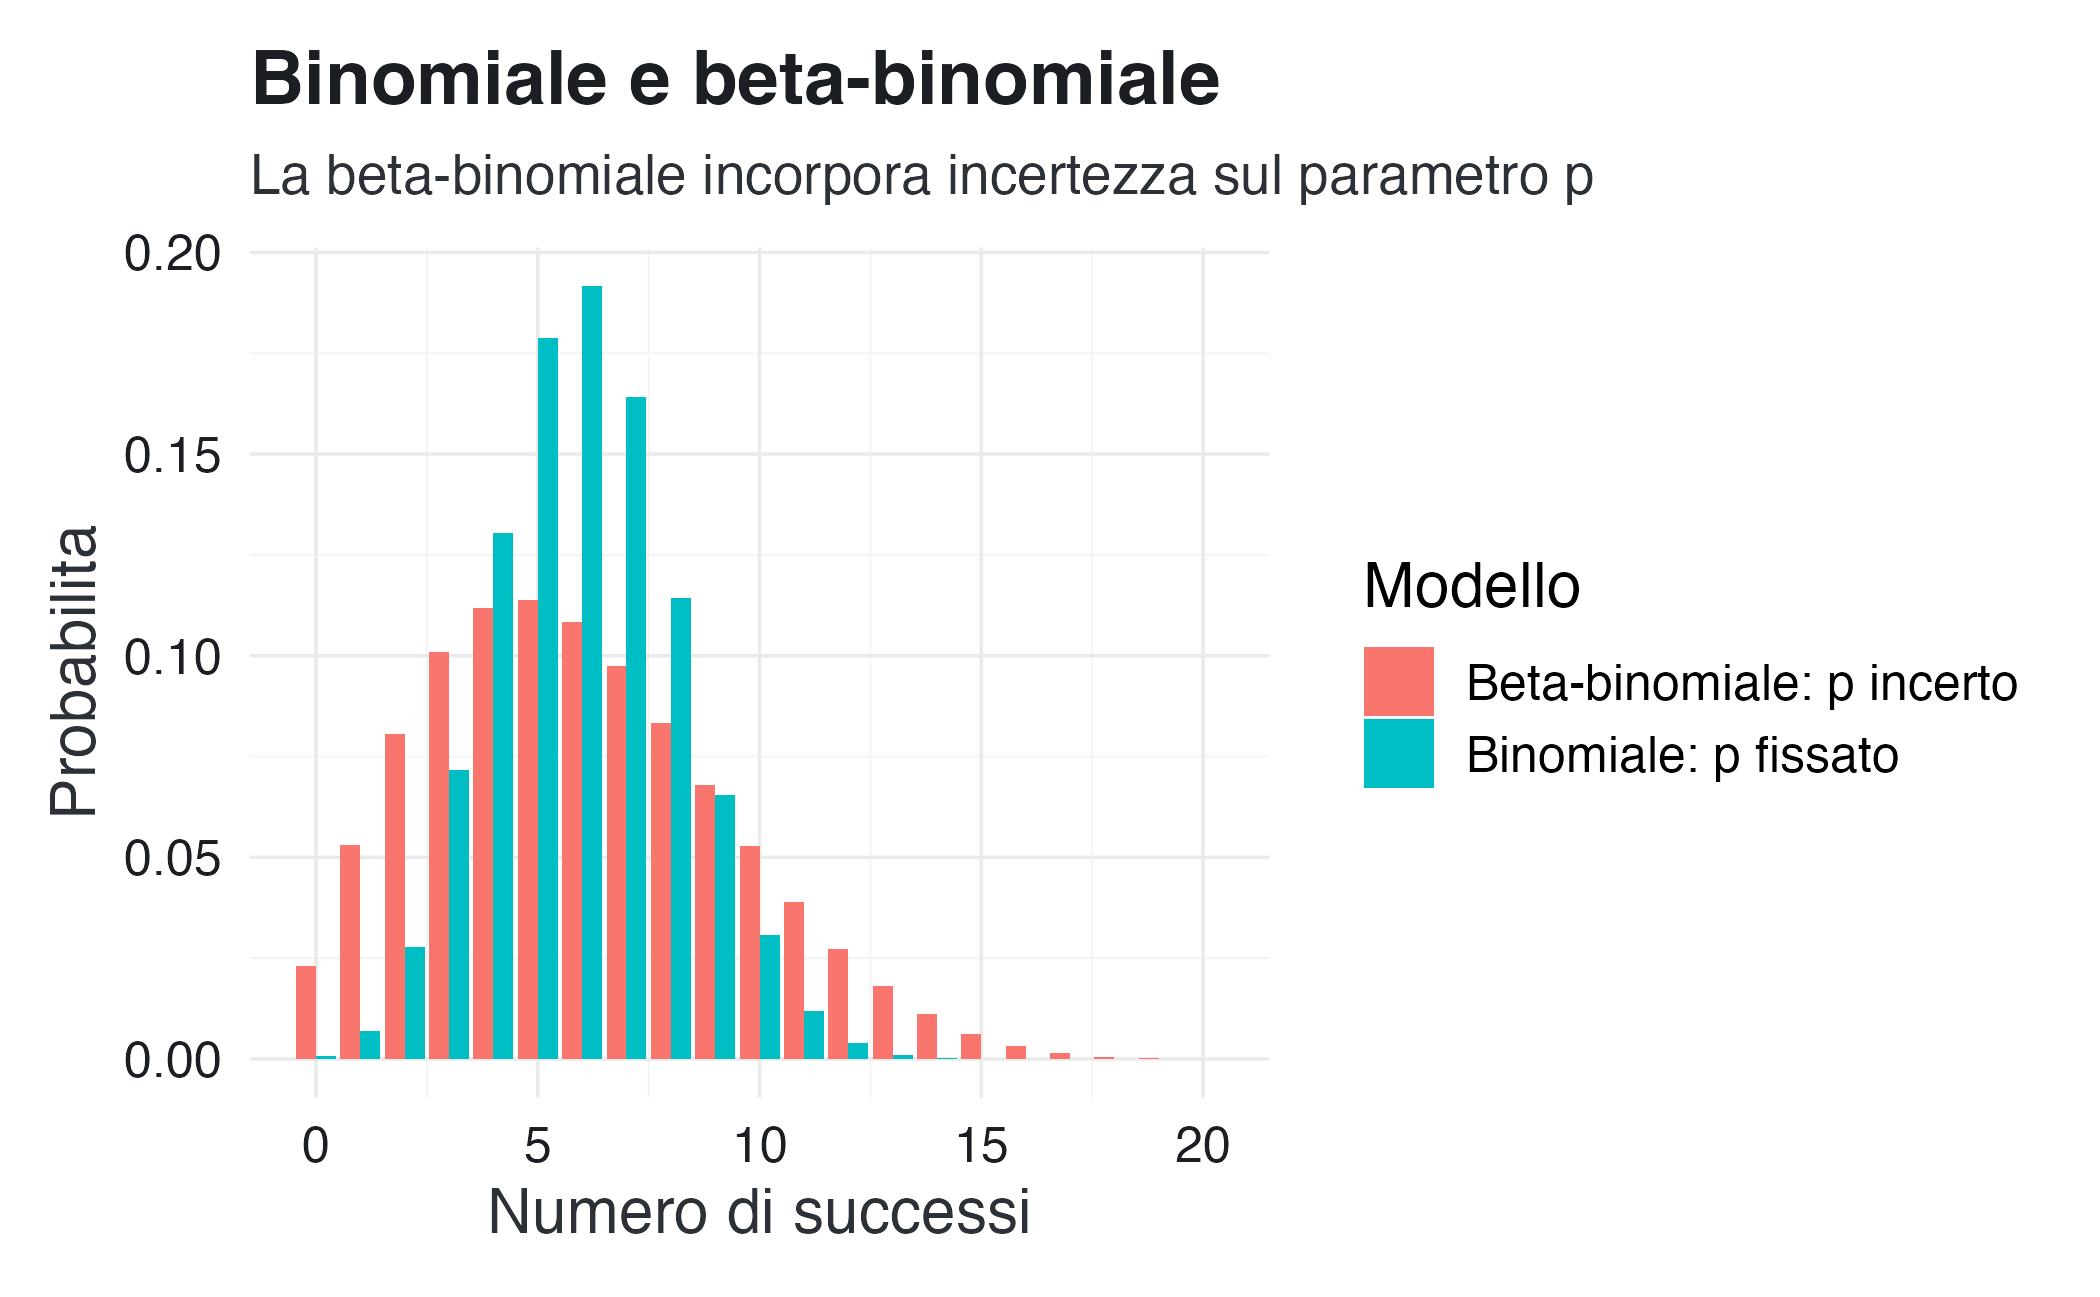
\includegraphics[width=0.85\linewidth,height=\textheight,keepaspectratio]{chapters/probability/11_discr_rv_distr_files/figure-pdf/unnamed-chunk-13-1.png}

Il modello predittivo è più disperso perché non si basa su un unico
valore di \(p\), ma integra diversi valori possibili, ponderati dalla
distribuzione Beta.

\end{tcolorbox}

\section*{Riflessioni conclusive}\label{riflessioni-conclusive-10}

\markright{Riflessioni conclusive}

Le distribuzioni discrete introdotte in questo capitolo costituiscono il
primo vocabolario dei modelli probabilistici per i dati psicologici. La
distribuzione uniforme discreta rappresenta scelte simmetriche tra
alternative finite, la distribuzione di Bernoulli modella un singolo
esito binario, la distribuzione binomiale modella il numero di successi
in un insieme di prove e la distribuzione di Poisson modella il
conteggio degli eventi in un intervallo.

In prospettiva bayesiana, questi modelli non sono semplici formule per
calcolare probabilità. Sono, piuttosto, dei modi per esplicitare le
assunzioni sul processo di generazione dei dati. Una volta osservati i
dati, le stesse distribuzioni potranno essere lette come
verosimiglianze, ovvero come funzioni che indicano quali valori dei
parametri rendono più o meno plausibili le osservazioni.

Il passo successivo sarà lo studio delle distribuzioni continue. Queste
distribuzioni saranno importanti sia per modellare variabili osservabili
continue, sia per rappresentare l'incertezza sui parametri dei modelli
discreti: la distribuzione Beta per probabilità come \(p\), la
distribuzione Gamma per i tassi come \(\lambda\), la distribuzione
Normale per le medie e le differenze.

\subsection*{Guida rapida: quale distribuzione
usare?}\label{guida-rapida-quale-distribuzione-usare}

{\def\LTcaptype{none} % do not increment counter
\begin{longtable}[]{@{}
  >{\raggedright\arraybackslash}p{(\linewidth - 8\tabcolsep) * \real{0.2000}}
  >{\raggedright\arraybackslash}p{(\linewidth - 8\tabcolsep) * \real{0.2000}}
  >{\raggedright\arraybackslash}p{(\linewidth - 8\tabcolsep) * \real{0.2000}}
  >{\raggedright\arraybackslash}p{(\linewidth - 8\tabcolsep) * \real{0.2000}}
  >{\raggedright\arraybackslash}p{(\linewidth - 8\tabcolsep) * \real{0.2000}}@{}}
\toprule\noalign{}
\begin{minipage}[b]{\linewidth}\raggedright
Distribuzione
\end{minipage} & \begin{minipage}[b]{\linewidth}\raggedright
Supporto
\end{minipage} & \begin{minipage}[b]{\linewidth}\raggedright
Domanda modellata
\end{minipage} & \begin{minipage}[b]{\linewidth}\raggedright
Esempio psicologico
\end{minipage} & \begin{minipage}[b]{\linewidth}\raggedright
Parametro principale
\end{minipage} \\
\midrule\noalign{}
\endhead
\bottomrule\noalign{}
\endlastfoot
Uniforme discreta & \(\{1,\ldots,N\}\) & Quale alternativa viene scelta,
se tutte sono simmetriche? & Assegnazione casuale a condizioni &
\(N\) \\
Bernoulli & \(\{0,1\}\) & L'evento si verifica oppure no? & Risposta
corretta a un item & \(p\) \\
Binomiale & \(\{0,\ldots,n\}\) & Quanti successi su \(n\) prove? &
Numero di item corretti & \(n,p\) \\
Poisson & \(\{0,1,2,\ldots\}\) & Quanti eventi in un intervallo? &
Attacchi di panico in un mese & \(\lambda\) \\
\end{longtable}
}

\section*{Punti chiave da ricordare}\label{punti-chiave-da-ricordare-10}
\addcontentsline{toc}{section}{Punti chiave da ricordare}

\markright{Punti chiave da ricordare}

\begin{tcolorbox}[enhanced jigsaw, arc=.35mm, bottomrule=.15mm, bottomtitle=1mm, breakable, colback=white, colbacktitle=quarto-callout-important-color!10!white, colframe=quarto-callout-important-color-frame, coltitle=black, left=2mm, leftrule=.75mm, opacityback=0, opacitybacktitle=0.6, rightrule=.15mm, title=\textcolor{quarto-callout-important-color}{\faExclamation}\hspace{0.5em}{Importante}, titlerule=0mm, toprule=.15mm, toptitle=1mm]

\begin{enumerate}
\def\labelenumi{\arabic{enumi}.}
\item
  \textbf{Una distribuzione discreta assegna probabilita a valori
  numerabili.} La somma delle probabilita su tutti i valori possibili
  deve essere uguale a 1.
\item
  \textbf{La Bernoulli modella un singolo esito binario.}

  \[
  P(X=x)=p^x(1-p)^{1-x}, \quad x\in\{0,1\}.
  \]
\item
  \textbf{La binomiale modella il numero di successi in \(n\) prove
  Bernoulli indipendenti.}

  \[
  P(Y=k)=\binom{n}{k}p^k(1-p)^{n-k}.
  \]
\item
  \textbf{La Poisson modella conteggi di eventi in un intervallo.}

  \[
  P(Y=y)=\frac{\lambda^y e^{-\lambda}}{y!}.
  \]
\item
  \textbf{Ogni distribuzione contiene assunzioni.} Bernoulli e binomiale
  assumono probabilita costante e indipendenza; la Poisson assume tasso
  costante ed equidispersione.
\item
  \textbf{Nel percorso bayesiano, il modello dei dati e condizionale al
  parametro.} Scrivere \(Y \mid \theta \sim p(y\mid\theta)\) non
  significa che \(\theta\) sia noto; significa che stiamo specificando
  cosa ci aspetteremmo di osservare per ciascun valore possibile di
  \(\theta\).
\end{enumerate}

\textbf{Per il prossimo capitolo:} nel
Capitolo~\ref{sec-prob-cont-distr} studieremo le distribuzioni continue,
fondamentali per rappresentare parametri incerti come probabilita,
tassi, medie e varianze.

\end{tcolorbox}

\section*{Esercizi}\label{esercizi-2}
\addcontentsline{toc}{section}{Esercizi}

\markright{Esercizi}

\begin{tcolorbox}[enhanced jigsaw, arc=.35mm, bottomrule=.15mm, bottomtitle=1mm, breakable, colback=white, colbacktitle=quarto-callout-important-color!10!white, colframe=quarto-callout-important-color-frame, coltitle=black, left=2mm, leftrule=.75mm, opacityback=0, opacitybacktitle=0.6, rightrule=.15mm, title=\textcolor{quarto-callout-important-color}{\faExclamation}\hspace{0.5em}{Esercizi di base}, titlerule=0mm, toprule=.15mm, toptitle=1mm]

\begin{enumerate}
\def\labelenumi{\arabic{enumi}.}
\tightlist
\item
  Scegli un esempio psicologico per ciascuna distribuzione: Bernoulli,
  binomiale e Poisson.
\item
  Per ogni esempio, identifica il supporto della variabile casuale.
\item
  Simula 1000 osservazioni da ciascun modello e confronta media e
  varianza empiriche con quelle teoriche.
\item
  Spiega quali assunzioni sarebbero necessarie per usare una binomiale
  in un test di 20 item.
\item
  Trova un caso in cui una Poisson potrebbe essere inadeguata perche la
  varianza e maggiore della media.
\end{enumerate}

\end{tcolorbox}

\begin{tcolorbox}[enhanced jigsaw, arc=.35mm, bottomrule=.15mm, bottomtitle=1mm, breakable, colback=white, colbacktitle=quarto-callout-caution-color!10!white, colframe=quarto-callout-caution-color-frame, coltitle=black, left=2mm, leftrule=.75mm, opacityback=0, opacitybacktitle=0.6, rightrule=.15mm, title=\textcolor{quarto-callout-caution-color}{\faFire}\hspace{0.5em}{Informazioni sull'ambiente di sviluppo}, titlerule=0mm, toprule=.15mm, toptitle=1mm]

\begin{Shaded}
\begin{Highlighting}[]
\FunctionTok{sessionInfo}\NormalTok{()}
\CommentTok{\#\textgreater{} R version 4.6.1 (2026{-}06{-}24)}
\CommentTok{\#\textgreater{} Platform: aarch64{-}apple{-}darwin23}
\CommentTok{\#\textgreater{} Running under: macOS Tahoe 26.5.2}
\CommentTok{\#\textgreater{} }
\CommentTok{\#\textgreater{} Matrix products: default}
\CommentTok{\#\textgreater{} BLAS:   /Library/Frameworks/R.framework/Versions/4.6/Resources/lib/libRblas.0.dylib }
\CommentTok{\#\textgreater{} LAPACK: /Library/Frameworks/R.framework/Versions/4.6/Resources/lib/libRlapack.dylib;  LAPACK version 3.12.1}
\CommentTok{\#\textgreater{} }
\CommentTok{\#\textgreater{} locale:}
\CommentTok{\#\textgreater{} [1] C.UTF{-}8/UTF{-}8/C.UTF{-}8/C/C.UTF{-}8/C.UTF{-}8}
\CommentTok{\#\textgreater{} }
\CommentTok{\#\textgreater{} time zone: Europe/Rome}
\CommentTok{\#\textgreater{} tzcode source: internal}
\CommentTok{\#\textgreater{} }
\CommentTok{\#\textgreater{} attached base packages:}
\CommentTok{\#\textgreater{} [1] stats     graphics  grDevices utils     datasets  methods   base     }
\CommentTok{\#\textgreater{} }
\CommentTok{\#\textgreater{} other attached packages:}
\CommentTok{\#\textgreater{}  [1] ragg\_1.5.2            tinytable\_0.17.0      withr\_3.0.3          }
\CommentTok{\#\textgreater{}  [4] systemfonts\_1.3.2     patchwork\_1.3.2       ggdist\_3.3.3         }
\CommentTok{\#\textgreater{}  [7] tidybayes\_3.0.7       bayesplot\_1.15.0      ggplot2\_4.0.3        }
\CommentTok{\#\textgreater{} [10] reliabilitydiag\_0.2.1 priorsense\_1.2.0      posterior\_1.7.0      }
\CommentTok{\#\textgreater{} [13] loo\_2.10.0            rstan\_2.32.7          StanHeaders\_2.32.10  }
\CommentTok{\#\textgreater{} [16] brms\_2.23.0           Rcpp\_1.1.2            sessioninfo\_1.2.4    }
\CommentTok{\#\textgreater{} [19] conflicted\_1.2.0      janitor\_2.2.1         matrixStats\_1.5.0    }
\CommentTok{\#\textgreater{} [22] modelr\_0.1.11         tibble\_3.3.1          dplyr\_1.2.1          }
\CommentTok{\#\textgreater{} [25] tidyr\_1.3.2           rio\_1.3.0             here\_1.0.2           }
\CommentTok{\#\textgreater{} }
\CommentTok{\#\textgreater{} loaded via a namespace (and not attached):}
\CommentTok{\#\textgreater{}  [1] svUnit\_1.0.8          tidyselect\_1.2.1      farver\_2.1.2         }
\CommentTok{\#\textgreater{}  [4] S7\_0.2.2              fastmap\_1.2.0         tensorA\_0.36.2.1     }
\CommentTok{\#\textgreater{}  [7] digest\_0.6.39         timechange\_0.4.0      estimability\_2.0.0   }
\CommentTok{\#\textgreater{} [10] lifecycle\_1.0.5       magrittr\_2.0.5        compiler\_4.6.1       }
\CommentTok{\#\textgreater{} [13] rlang\_1.3.0           tools\_4.6.1           knitr\_1.51           }
\CommentTok{\#\textgreater{} [16] labeling\_0.4.3        bridgesampling\_1.2{-}1  pkgbuild\_1.4.8       }
\CommentTok{\#\textgreater{} [19] curl\_7.1.0            RColorBrewer\_1.1{-}3    abind\_1.4{-}8          }
\CommentTok{\#\textgreater{} [22] purrr\_1.2.2           grid\_4.6.1            stats4\_4.6.1         }
\CommentTok{\#\textgreater{} [25] xtable\_1.8{-}8          inline\_0.3.21         emmeans\_2.0.3        }
\CommentTok{\#\textgreater{} [28] scales\_1.4.0          cli\_3.6.6             mvtnorm\_1.4{-}1        }
\CommentTok{\#\textgreater{} [31] rmarkdown\_2.31        generics\_0.1.4        otel\_0.2.0           }
\CommentTok{\#\textgreater{} [34] RcppParallel\_5.1.11{-}2 cachem\_1.1.0          stringr\_1.6.0        }
\CommentTok{\#\textgreater{} [37] parallel\_4.6.1        vctrs\_0.7.3           V8\_8.2.0             }
\CommentTok{\#\textgreater{} [40] Matrix\_1.7{-}5          jsonlite\_2.0.0        arrayhelpers\_1.1{-}1   }
\CommentTok{\#\textgreater{} [43] glue\_1.8.1            codetools\_0.2{-}20      distributional\_0.8.1 }
\CommentTok{\#\textgreater{} [46] lubridate\_1.9.5       stringi\_1.8.7         gtable\_0.3.6         }
\CommentTok{\#\textgreater{} [49] QuickJSR\_1.10.0       pillar\_1.11.1         htmltools\_0.5.9      }
\CommentTok{\#\textgreater{} [52] Brobdingnag\_1.2{-}9     R6\_2.6.1              textshaping\_1.0.5    }
\CommentTok{\#\textgreater{} [55] rprojroot\_2.1.1       evaluate\_1.0.5        lattice\_0.22{-}9       }
\CommentTok{\#\textgreater{} [58] backports\_1.5.1       memoise\_2.0.1         broom\_1.0.13         }
\CommentTok{\#\textgreater{} [61] snakecase\_0.11.1      rstantools\_2.6.0      coda\_0.19{-}4.1        }
\CommentTok{\#\textgreater{} [64] gridExtra\_2.3.1       nlme\_3.1{-}169          checkmate\_2.3.4      }
\CommentTok{\#\textgreater{} [67] xfun\_0.60             pkgconfig\_2.0.3}
\end{Highlighting}
\end{Shaded}

\end{tcolorbox}

\section*{Bibliografia}\label{bibliografia-5}

\markright{Bibliografia}

\chapter{Distribuzioni di variabili casuali
continue}\label{sec-prob-cont-distr}

\section*{Introduzione}\label{introduzione-11}

\markright{Introduzione}

Nel 2 abbiamo considerato variabili con valori numerabili: risposte
corrette/errate, numero di successi, conteggi. Qui passiamo alle
\textbf{variabili casuali continue}, che si muovono su una scala
numerica: punteggi psicometrici, tempi di risposta, durate, tassi,
proporzioni, effetti medi e differenze fra gruppi.

La differenza chiave è che nel continuo la probabilità non si assegna ai
singoli valori, ma agli \textbf{intervalli}. Per \(X\) è continua,

\[
P(X = x) = 0,
\] ha senso, invece,

\[
P(a \leq X \leq b).
\] data dall'\textbf{area sotto la curva di densità} tra \(a\) e \(b\).

Restiamo qui in un'ottica bayesiana, ma senza svolgere ancora
l'inferenza completa. Come nel capitolo precedente, l'obiettivo è
riconoscere le principali famiglie di modelli generativi continui e il
loro ruolo nel ragionamento probabilistico.

Una distribuzione continua può svolgere almeno tre ruoli:

\begin{enumerate}
\def\labelenumi{\arabic{enumi}.}
\tightlist
\item
  \begin{itemize}
  \tightlist
  \item
    modello dei dati osservabili: per esempio, normale per gli errori di
    misura, gamma per i tempi positivi e asimmetrici;\\
  \end{itemize}
\item
  \begin{itemize}
  \tightlist
  \item
    prior per parametri continui: per esempio, beta per una probabilità,
    gamma per un tasso, normale per un effetto;\\
  \end{itemize}
\item
  \begin{itemize}
  \tightlist
  \item
    componente di verosimiglianza: quando, dopo l'osservazione, lo
    stesso modello serve a individuare quali valori del parametro
    rendano i dati più plausibili.
  \end{itemize}
\end{enumerate}

In questo capitolo ci concentreremo soprattutto sui primi due; il terzo
sarà formalizzato nel Capitolo~\ref{sec-prob-likelihood}, dopo il
capitolo-ponte Capitolo~\ref{sec-prob-inference-uncertainty}.

In questo capitolo:

\begin{enumerate}
\def\labelenumi{\arabic{enumi}.}
\tightlist
\item
  \textbf{chiariremo} il significato di densita, supporto e probabilita
  come area;
\item
  \textbf{richiameremo} le funzioni R per lavorare con distribuzioni
  continue;
\item
  \textbf{studieremo} le distribuzioni uniforme, normale, esponenziale e
  gamma;
\item
  \textbf{introdurremo} la distribuzione beta come modello naturale per
  probabilita e proporzioni;
\item
  \textbf{discuteremo} le distribuzioni chi-quadrato, \(t\) di Student e
  Cauchy come distribuzioni derivate o robuste;
\item
  \textbf{collegheremo} ogni distribuzione al suo ruolo nel percorso
  bayesiano complessivo.
\end{enumerate}

\begin{tcolorbox}[enhanced jigsaw, arc=.35mm, bottomrule=.15mm, bottomtitle=1mm, breakable, colback=white, colbacktitle=quarto-callout-tip-color!10!white, colframe=quarto-callout-tip-color-frame, coltitle=black, left=2mm, leftrule=.75mm, opacityback=0, opacitybacktitle=0.6, rightrule=.15mm, title=\textcolor{quarto-callout-tip-color}{\faLightbulb}\hspace{0.5em}{Prerequisiti}, titlerule=0mm, toprule=.15mm, toptitle=1mm]

Per seguire questo capitolo e utile aver letto:

\begin{itemize}
\tightlist
\item
  Capitolo~\ref{sec-prob-random-var};
\item
  Capitolo~\ref{sec-prob-distr};
\item
  Capitolo~\ref{sec-prob-random-var-properties};
\item
  1;
\item
  \begin{enumerate}
  \def\labelenumi{\arabic{enumi}.}
  \setcounter{enumi}{1}
  \tightlist
  \item
  \end{enumerate}
\end{itemize}

Il richiamo più importante è il concetto di \textbf{funzione di
densita}: nel caso continuo, la probabilità di un intervallo è un'area
sotto la curva.

\end{tcolorbox}

\begin{tcolorbox}[enhanced jigsaw, arc=.35mm, bottomrule=.15mm, bottomtitle=1mm, breakable, colback=white, colbacktitle=quarto-callout-caution-color!10!white, colframe=quarto-callout-caution-color-frame, coltitle=black, left=2mm, leftrule=.75mm, opacityback=0, opacitybacktitle=0.6, rightrule=.15mm, title=\textcolor{quarto-callout-caution-color}{\faFire}\hspace{0.5em}{Preparazione del Notebook}, titlerule=0mm, toprule=.15mm, toptitle=1mm]

\begin{Shaded}
\begin{Highlighting}[]
\NormalTok{here}\SpecialCharTok{::}\FunctionTok{here}\NormalTok{(}\StringTok{"code"}\NormalTok{, }\StringTok{"\_common.R"}\NormalTok{) }\SpecialCharTok{|\textgreater{}}
  \FunctionTok{source}\NormalTok{()}

\CommentTok{\# Riapplica il tema per sicurezza, se definito nel progetto.}
\FunctionTok{apply\_visual\_theme}\NormalTok{()}
\end{Highlighting}
\end{Shaded}

\end{tcolorbox}

\section{Che cosa descrive una distribuzione
continua?}\label{sec-continuous-distribution-meaning}

Una distribuzione continua descrive una variabile casuale che può
assumere valori in un intervallo della retta reale. La distribuzione è
rappresentata da una \textbf{funzione di densità} \(f(x)\).

La densità deve soddisfare due condizioni:

\[
f(x) \geq 0,
\qquad
\int_{-\infty}^{+\infty} f(x)\,dx = 1.
\]

La probabilità che \(X\) cada in un intervallo \([a,b]\) è:

\[
P(a \leq X \leq b) = \int_a^b f(x)\,dx.
\]

\begin{tcolorbox}[enhanced jigsaw, arc=.35mm, bottomrule=.15mm, bottomtitle=1mm, breakable, colback=white, colbacktitle=quarto-callout-important-color!10!white, colframe=quarto-callout-important-color-frame, coltitle=black, left=2mm, leftrule=.75mm, opacityback=0, opacitybacktitle=0.6, rightrule=.15mm, title=\textcolor{quarto-callout-important-color}{\faExclamation}\hspace{0.5em}{Densita non significa probabilita puntuale}, titlerule=0mm, toprule=.15mm, toptitle=1mm]

Per una variabile continua, il valore \(f(x)\) non è una probabilità.
Può anche essere maggiore di 1. La probabilità è sempre un'area sotto la
curva, cioè l'integrale della densità su un intervallo.

Questa distinzione sarà importante nel capitolo sulla verosimiglianza:
una densità può essere usata per confrontare valori del parametro, ma
non deve essere confusa con una probabilità assegnata a un singolo
punto.

\end{tcolorbox}

\subsection{Supporto della
distribuzione}\label{supporto-della-distribuzione}

Il \textbf{supporto} è l'insieme dei valori che una variabile può
assumere. Alcuni esempi:

{\def\LTcaptype{none} % do not increment counter
\begin{longtable}[]{@{}
  >{\raggedright\arraybackslash}p{(\linewidth - 4\tabcolsep) * \real{0.3000}}
  >{\raggedleft\arraybackslash}p{(\linewidth - 4\tabcolsep) * \real{0.4000}}
  >{\raggedright\arraybackslash}p{(\linewidth - 4\tabcolsep) * \real{0.3000}}@{}}
\toprule\noalign{}
\begin{minipage}[b]{\linewidth}\raggedright
Distribuzione
\end{minipage} & \begin{minipage}[b]{\linewidth}\raggedleft
Supporto
\end{minipage} & \begin{minipage}[b]{\linewidth}\raggedright
Uso tipico
\end{minipage} \\
\midrule\noalign{}
\endhead
\bottomrule\noalign{}
\endlastfoot
Uniforme\((a,b)\) & \([a,b]\) & parametro limitato a un intervallo \\
Normale\((\mu,\sigma^2)\) & \(\mathbb{R}\) & misure simmetriche, errori
additivi, effetti \\
Esponenziale\((\lambda)\) & \((0,\infty)\) & tempi di attesa con tasso
costante \\
Gamma\((\alpha,\beta)\) & \((0,\infty)\) & tempi, tassi, precisioni \\
Beta\((\alpha,\beta)\) & \((0,1)\) & probabilita e proporzioni \\
\(t_\nu\) & \(\mathbb{R}\) & effetti continui con code pesanti \\
Cauchy\((x_0,s)\) & \(\mathbb{R}\) & prior robuste molto deboli \\
\end{longtable}
}

La prima domanda pratica, quando scegliamo una distribuzione, è quindi:
\textbf{Quali valori sono possibili per la variabile o per il
parametro?}

\section{Le funzioni R per le distribuzioni
continue}\label{sec-r-continuous-functions}

R usa la stessa convenzione vista per le distribuzioni discrete. Ogni
famiglia ha quattro funzioni principali:

{\def\LTcaptype{none} % do not increment counter
\begin{longtable}[]{@{}lll@{}}
\toprule\noalign{}
Prefisso & Significato & Esempio con la normale \\
\midrule\noalign{}
\endhead
\bottomrule\noalign{}
\endlastfoot
\texttt{d} & densita & \texttt{dnorm(x,\ mean,\ sd)} \\
\texttt{p} & probabilita cumulata & \texttt{pnorm(x,\ mean,\ sd)} \\
\texttt{q} & quantile & \texttt{qnorm(p,\ mean,\ sd)} \\
\texttt{r} & generazione casuale & \texttt{rnorm(n,\ mean,\ sd)} \\
\end{longtable}
}

Esempio: consideriamo punteggi standardizzati approssimativamente
distribuiti come

\[
X \sim \mathcal{N}(100, 15^2).
\]

\begin{Shaded}
\begin{Highlighting}[]
\NormalTok{mu }\OtherTok{\textless{}{-}} \DecValTok{100}
\NormalTok{sigma }\OtherTok{\textless{}{-}} \DecValTok{15}

\CommentTok{\# Densita nel punto 100: non e una probabilita puntuale.}
\NormalTok{densita\_100 }\OtherTok{\textless{}{-}} \FunctionTok{dnorm}\NormalTok{(}\DecValTok{100}\NormalTok{, }\AttributeTok{mean =}\NormalTok{ mu, }\AttributeTok{sd =}\NormalTok{ sigma)}

\CommentTok{\# Probabilita di osservare un punteggio tra 85 e 115.}
\NormalTok{prob\_85\_115 }\OtherTok{\textless{}{-}} \FunctionTok{pnorm}\NormalTok{(}\DecValTok{115}\NormalTok{, }\AttributeTok{mean =}\NormalTok{ mu, }\AttributeTok{sd =}\NormalTok{ sigma) }\SpecialCharTok{{-}}
  \FunctionTok{pnorm}\NormalTok{(}\DecValTok{85}\NormalTok{, }\AttributeTok{mean =}\NormalTok{ mu, }\AttributeTok{sd =}\NormalTok{ sigma)}

\CommentTok{\# Quantile che lascia sotto di se il 95\% della distribuzione.}
\NormalTok{q\_95 }\OtherTok{\textless{}{-}} \FunctionTok{qnorm}\NormalTok{(}\FloatTok{0.95}\NormalTok{, }\AttributeTok{mean =}\NormalTok{ mu, }\AttributeTok{sd =}\NormalTok{ sigma)}

\CommentTok{\# Cinque valori simulati.}
\NormalTok{simulazioni }\OtherTok{\textless{}{-}} \FunctionTok{rnorm}\NormalTok{(}\DecValTok{5}\NormalTok{, }\AttributeTok{mean =}\NormalTok{ mu, }\AttributeTok{sd =}\NormalTok{ sigma)}

\NormalTok{densita\_100}
\CommentTok{\#\textgreater{} [1] 0.0266}
\NormalTok{prob\_85\_115}
\CommentTok{\#\textgreater{} [1] 0.683}
\NormalTok{q\_95}
\CommentTok{\#\textgreater{} [1] 125}
\NormalTok{simulazioni}
\CommentTok{\#\textgreater{} [1]  76.7  94.6 107.4 111.8 110.2}
\end{Highlighting}
\end{Shaded}

\begin{tcolorbox}[enhanced jigsaw, arc=.35mm, bottomrule=.15mm, bottomtitle=1mm, breakable, colback=white, colbacktitle=quarto-callout-note-color!10!white, colframe=quarto-callout-note-color-frame, coltitle=black, left=2mm, leftrule=.75mm, opacityback=0, opacitybacktitle=0.6, rightrule=.15mm, title=\textcolor{quarto-callout-note-color}{\faInfo}\hspace{0.5em}{Una lettura bayesiana delle simulazioni}, titlerule=0mm, toprule=.15mm, toptitle=1mm]

Quando usiamo funzioni come \texttt{rnorm()} o \texttt{rgamma()}, non
stiamo solo producendo numeri casuali. Stiamo simulando dati o parametri
\textbf{sotto un modello}. Questa abitudine sarà utile nei capitoli
successivi: simulare da una prior, da una distribuzione predittiva o da
una posterior permette di rendere visibile l'incertezza.

\end{tcolorbox}

\section{Distribuzione uniforme continua}\label{sec-cont-uniform}

\subsection{Definizione}\label{definizione-4}

La distribuzione uniforme continua assegna la stessa densità a tutti i
valori di un intervallo finito \([a,b]\).

\begin{definition}[]\protect\hypertarget{def-uniform-cont}{}\label{def-uniform-cont}

Una variabile casuale \(X\) segue una distribuzione uniforme continua su
\([a,b]\) se

\[
X \sim \mathrm{Uniforme}(a,b),
\qquad
f(x) = \frac{1}{b-a}, \quad a \leq x \leq b,
\] mentre \(f(x)=0\) fuori dall'intervallo.

Le proprietà principali sono:

\[
\mathbb{E}(X) = \frac{a+b}{2},
\qquad
\mathbb{V}(X) = \frac{(b-a)^2}{12}.
\]

\end{definition}

\subsection{Interpretazione}\label{interpretazione}

La distribuzione uniforme rappresenta una forma di \textbf{indifferenza
locale}: dato un intervallo, nessun sottointervallo di uguale lunghezza
è ritenuto più plausibile di un altro.

Ad esempio, se prima di osservare dati riteniamo plausibile che una
probabilità possa assumere qualunque valore tra 0 e 1, possiamo usare

\[
\theta \sim \mathrm{Uniforme}(0,1).
\]

Questa scelta coincide con una distribuzione \(\mathrm{Beta}(1,1)\).

\begin{tcolorbox}[enhanced jigsaw, arc=.35mm, bottomrule=.15mm, bottomtitle=1mm, breakable, colback=white, colbacktitle=quarto-callout-warning-color!10!white, colframe=quarto-callout-warning-color-frame, coltitle=black, left=2mm, leftrule=.75mm, opacityback=0, opacitybacktitle=0.6, rightrule=.15mm, title=\textcolor{quarto-callout-warning-color}{\faExclamationTriangle}\hspace{0.5em}{La prior uniforme non e sempre neutrale}, titlerule=0mm, toprule=.15mm, toptitle=1mm]

Una prior uniforme può sembrare non informativa, ma non è
automaticamente neutrale. La sua forma dipende dalla scala scelta. Una
prior uniforme su \(\theta\) non corrisponde a una prior uniforme su una
trasformazione non lineare, come \(\log(\theta)\) o \(\theta^2\).

Inoltre, una distribuzione uniforme su un intervallo finito esclude a
priori tutti i valori fuori da quell'intervallo. Questa puo essere una
scelta ragionevole solo se il vincolo è davvero parte del problema.

\end{tcolorbox}

\subsection{Probabilita come lunghezza
relativa}\label{probabilita-come-lunghezza-relativa}

Per \(X \sim \mathrm{Uniforme}(a,b)\),

\[
P(c \leq X \leq d) = \frac{d-c}{b-a},
\qquad a \leq c < d \leq b.
\]

\begin{Shaded}
\begin{Highlighting}[]
\CommentTok{\# Esempio: uno spinner su un intervallo da 0 a 360 gradi.}
\NormalTok{prob }\OtherTok{\textless{}{-}} \FunctionTok{punif}\NormalTok{(}\DecValTok{250}\NormalTok{, }\AttributeTok{min =} \DecValTok{0}\NormalTok{, }\AttributeTok{max =} \DecValTok{360}\NormalTok{) }\SpecialCharTok{{-}}
  \FunctionTok{punif}\NormalTok{(}\DecValTok{150}\NormalTok{, }\AttributeTok{min =} \DecValTok{0}\NormalTok{, }\AttributeTok{max =} \DecValTok{360}\NormalTok{)}

\NormalTok{prob}
\CommentTok{\#\textgreater{} [1] 0.278}
\end{Highlighting}
\end{Shaded}

\begin{Shaded}
\begin{Highlighting}[]
\NormalTok{x }\OtherTok{\textless{}{-}} \FunctionTok{seq}\NormalTok{(}\DecValTok{0}\NormalTok{, }\DecValTok{360}\NormalTok{, }\AttributeTok{length.out =} \DecValTok{500}\NormalTok{)}
\NormalTok{df\_unif }\OtherTok{\textless{}{-}} \FunctionTok{data.frame}\NormalTok{(}
  \AttributeTok{x =}\NormalTok{ x,}
  \AttributeTok{densita =} \FunctionTok{dunif}\NormalTok{(x, }\AttributeTok{min =} \DecValTok{0}\NormalTok{, }\AttributeTok{max =} \DecValTok{360}\NormalTok{),}
  \AttributeTok{area =}\NormalTok{ x }\SpecialCharTok{\textgreater{}=} \DecValTok{150} \SpecialCharTok{\&}\NormalTok{ x }\SpecialCharTok{\textless{}=} \DecValTok{250}
\NormalTok{)}

\FunctionTok{ggplot}\NormalTok{(df\_unif, }\FunctionTok{aes}\NormalTok{(}\AttributeTok{x =}\NormalTok{ x, }\AttributeTok{y =}\NormalTok{ densita)) }\SpecialCharTok{+}
  \FunctionTok{geom\_line}\NormalTok{(}\AttributeTok{linewidth =} \DecValTok{1}\NormalTok{) }\SpecialCharTok{+}
  \FunctionTok{geom\_area}\NormalTok{(}
    \AttributeTok{data =} \FunctionTok{subset}\NormalTok{(df\_unif, area),}
    \AttributeTok{alpha =} \FloatTok{0.4}
\NormalTok{  ) }\SpecialCharTok{+}
  \FunctionTok{labs}\NormalTok{(}
    \AttributeTok{title =} \StringTok{"Distribuzione uniforme continua"}\NormalTok{,}
    \AttributeTok{subtitle =} \StringTok{"Area evidenziata: P(150 \textless{}= X \textless{}= 250)"}\NormalTok{,}
    \AttributeTok{x =} \StringTok{"Valore"}\NormalTok{,}
    \AttributeTok{y =} \StringTok{"Densita"}
\NormalTok{  )}
\end{Highlighting}
\end{Shaded}

\begin{center}
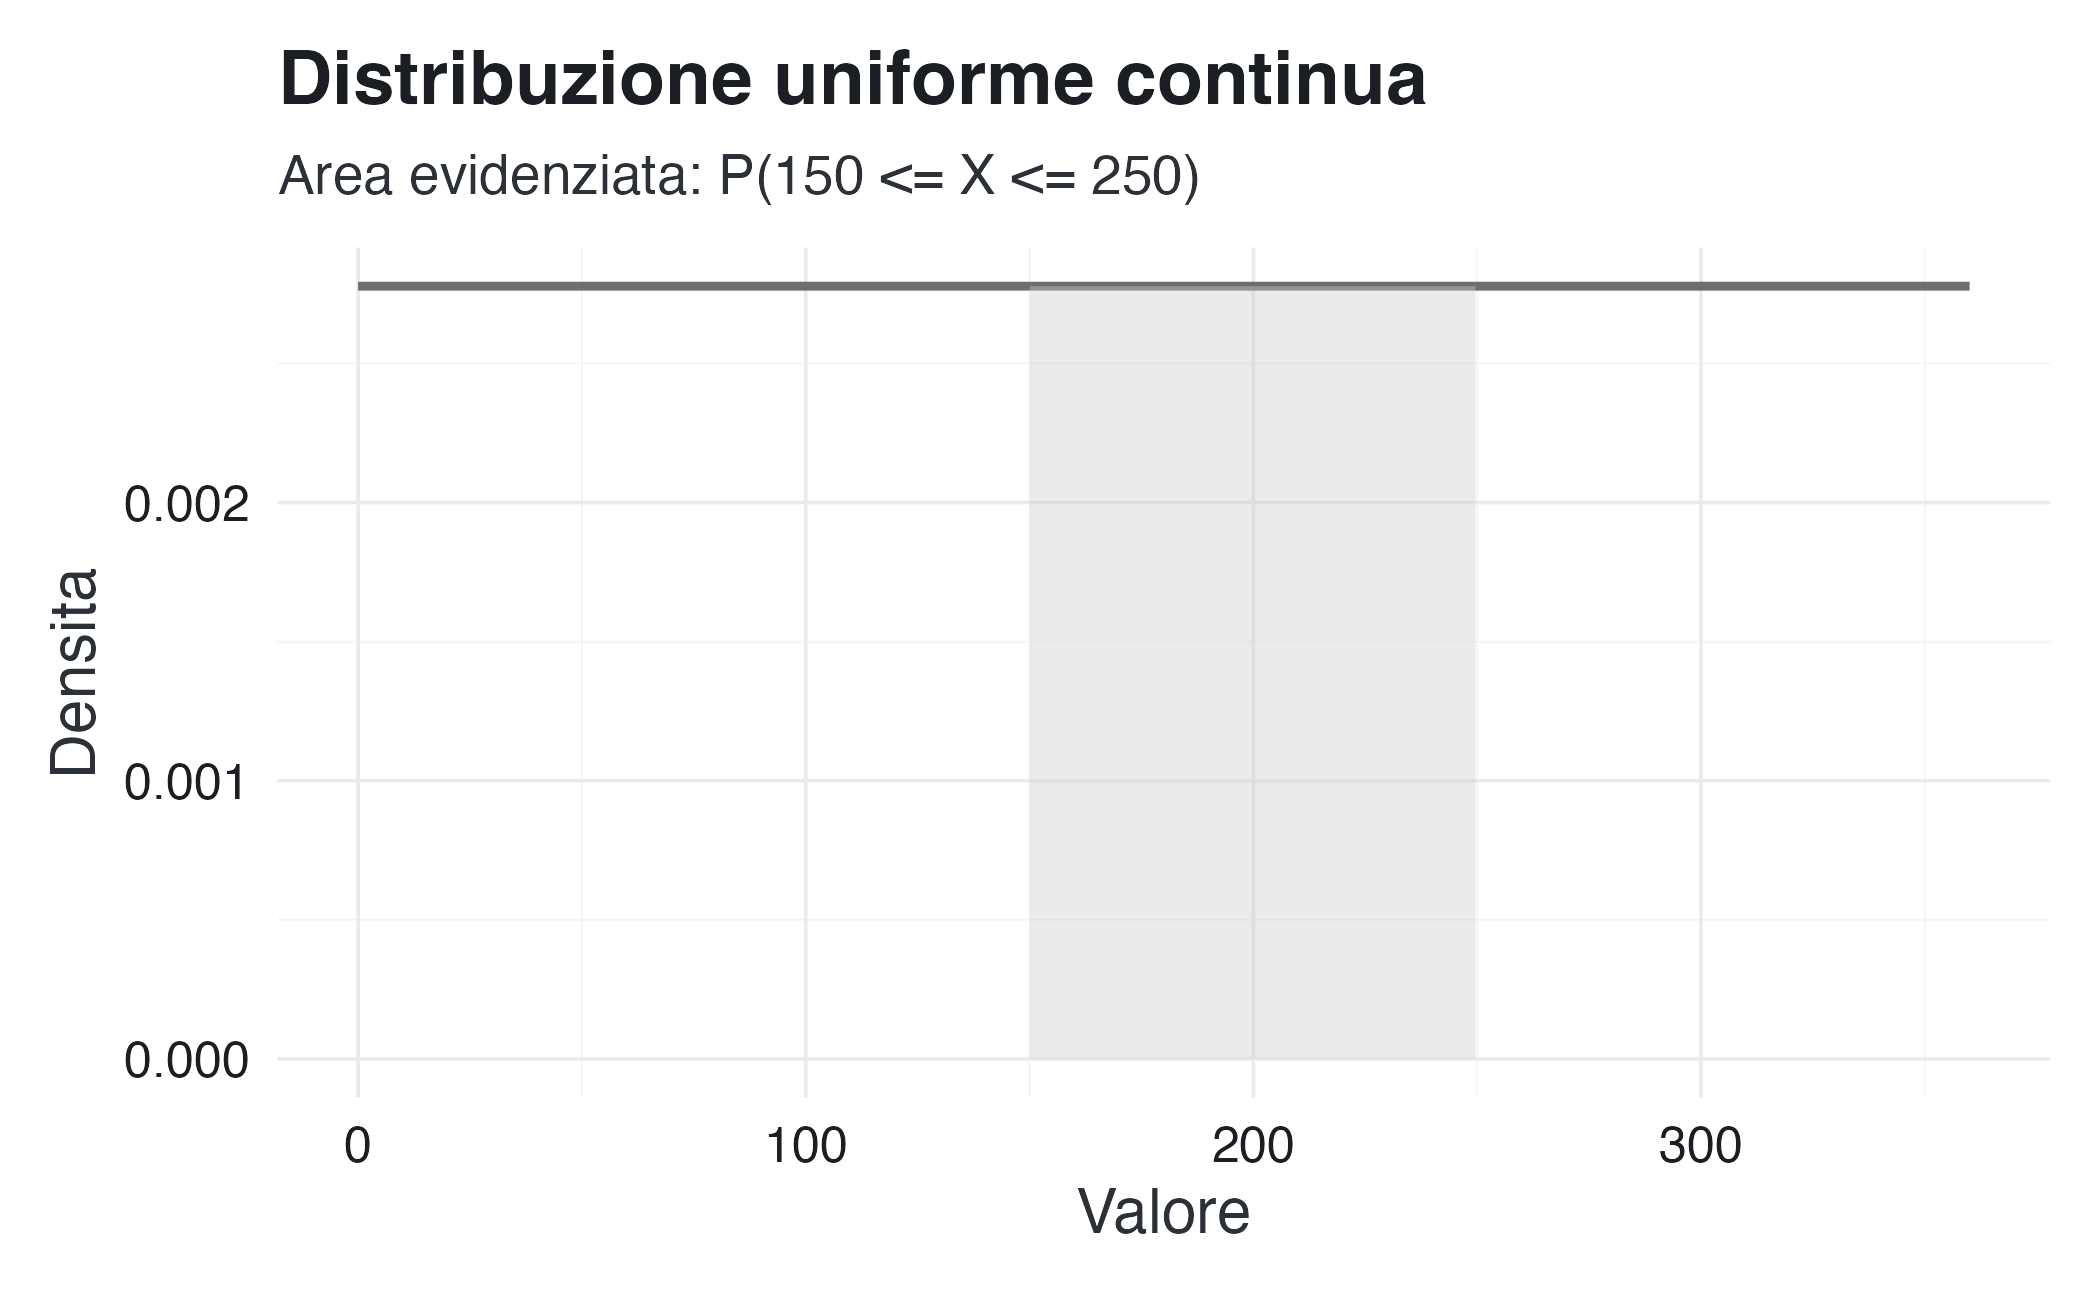
\includegraphics[width=0.85\linewidth,height=\textheight,keepaspectratio]{chapters/probability/12_cont_rv_distr_files/figure-pdf/unnamed-chunk-4-1.png}
\end{center}

\section{Distribuzione normale}\label{sec-cont-normal}

\subsection{Definizione}\label{definizione-5}

La distribuzione normale, o gaussiana, è una delle distribuzioni
continue più importanti. È adatta a rappresentare misure che variano
attorno a un centro e che hanno deviazioni approssimativamente
simmetriche.

\begin{definition}[]\protect\hypertarget{def-normal}{}\label{def-normal}

Una variabile casuale \(Y\) segue una distribuzione normale con media
\(\mu\) e deviazione standard \(\sigma > 0\) se

\[
Y \sim \mathcal{N}(\mu,\sigma^2),
\] con densità

\[
f(y) = \frac{1}{\sigma\sqrt{2\pi}}
\exp\left[-\frac{(y-\mu)^2}{2\sigma^2}\right].
\]

Le proprietà principali sono:

\[
\mathbb{E}(Y)=\mu,
\qquad
\mathbb{V}(Y)=\sigma^2.
\]

\end{definition}

\subsection{Interpretazione dei
parametri}\label{interpretazione-dei-parametri}

\begin{itemize}
\tightlist
\item
  \(\mu\) è il centro della distribuzione: valori maggiori di \(\mu\)
  spostano la curva verso destra, valori minori verso sinistra.
\item
  \(\sigma\) è la scala della variabilita: valori maggiori producono
  curve piu larghe e meno concentrate.
\end{itemize}

In psicologia, la normale è spesso un modello utile per punteggi
standardizzati, errori di misura, effetti continui e medie campionarie.
Va però usata come \textbf{approssimazione}, non come descrizione
automatica di qualunque fenomeno psicologico.

\begin{tcolorbox}[enhanced jigsaw, arc=.35mm, bottomrule=.15mm, bottomtitle=1mm, breakable, colback=white, colbacktitle=quarto-callout-note-color!10!white, colframe=quarto-callout-note-color-frame, coltitle=black, left=2mm, leftrule=.75mm, opacityback=0, opacitybacktitle=0.6, rightrule=.15mm, title=\textcolor{quarto-callout-note-color}{\faInfo}\hspace{0.5em}{Perche la normale e cosi importante?}, titlerule=0mm, toprule=.15mm, toptitle=1mm]

La normale compare spesso per due ragioni diverse:

\begin{enumerate}
\def\labelenumi{\arabic{enumi}.}
\tightlist
\item
  può essere un modello ragionevole per dati continui generati dalla
  somma di molte piccole influenze indipendenti;
\item
  nel Capitolo~\ref{sec-prob-inference-uncertainty} vedremo che, sotto
  condizioni generali, la media campionaria tende ad avere una
  distribuzione approssimativamente normale.
\end{enumerate}

La seconda ragione è legata al Teorema del Limite Centrale e sarà
discussa nel capitolo successivo.

\end{tcolorbox}

\subsection{Regola 68-95-99.7}\label{regola-68-95-99.7}

Per una distribuzione normale:

\begin{itemize}
\tightlist
\item
  circa il 68\% della massa si trova entro \(\mu \pm 1\sigma\);
\item
  circa il 95\% entro \(\mu \pm 1.96\sigma\);
\item
  circa il 99.7\% entro \(\mu \pm 3\sigma\).
\end{itemize}

\begin{Shaded}
\begin{Highlighting}[]
\NormalTok{mu }\OtherTok{\textless{}{-}} \DecValTok{100}
\NormalTok{sigma }\OtherTok{\textless{}{-}} \DecValTok{15}

\NormalTok{x }\OtherTok{\textless{}{-}} \FunctionTok{seq}\NormalTok{(mu }\SpecialCharTok{{-}} \DecValTok{4} \SpecialCharTok{*}\NormalTok{ sigma, mu }\SpecialCharTok{+} \DecValTok{4} \SpecialCharTok{*}\NormalTok{ sigma, }\AttributeTok{length.out =} \DecValTok{1000}\NormalTok{)}
\NormalTok{df\_norm }\OtherTok{\textless{}{-}} \FunctionTok{data.frame}\NormalTok{(}
  \AttributeTok{x =}\NormalTok{ x,}
  \AttributeTok{densita =} \FunctionTok{dnorm}\NormalTok{(x, }\AttributeTok{mean =}\NormalTok{ mu, }\AttributeTok{sd =}\NormalTok{ sigma),}
  \AttributeTok{centrale\_95 =}\NormalTok{ x }\SpecialCharTok{\textgreater{}=}\NormalTok{ mu }\SpecialCharTok{{-}} \FloatTok{1.96} \SpecialCharTok{*}\NormalTok{ sigma }\SpecialCharTok{\&}\NormalTok{ x }\SpecialCharTok{\textless{}=}\NormalTok{ mu }\SpecialCharTok{+} \FloatTok{1.96} \SpecialCharTok{*}\NormalTok{ sigma}
\NormalTok{)}

\FunctionTok{ggplot}\NormalTok{(df\_norm, }\FunctionTok{aes}\NormalTok{(}\AttributeTok{x =}\NormalTok{ x, }\AttributeTok{y =}\NormalTok{ densita)) }\SpecialCharTok{+}
  \FunctionTok{geom\_line}\NormalTok{(}\AttributeTok{linewidth =} \DecValTok{1}\NormalTok{) }\SpecialCharTok{+}
  \FunctionTok{geom\_area}\NormalTok{(}
    \AttributeTok{data =} \FunctionTok{subset}\NormalTok{(df\_norm, centrale\_95),}
    \AttributeTok{alpha =} \FloatTok{0.4}
\NormalTok{  ) }\SpecialCharTok{+}
  \FunctionTok{geom\_vline}\NormalTok{(}\AttributeTok{xintercept =}\NormalTok{ mu }\SpecialCharTok{{-}} \FloatTok{1.96} \SpecialCharTok{*}\NormalTok{ sigma, }\AttributeTok{linetype =} \StringTok{"dashed"}\NormalTok{) }\SpecialCharTok{+}
  \FunctionTok{geom\_vline}\NormalTok{(}\AttributeTok{xintercept =}\NormalTok{ mu }\SpecialCharTok{+} \FloatTok{1.96} \SpecialCharTok{*}\NormalTok{ sigma, }\AttributeTok{linetype =} \StringTok{"dashed"}\NormalTok{) }\SpecialCharTok{+}
  \FunctionTok{labs}\NormalTok{(}
    \AttributeTok{title =} \StringTok{"Distribuzione normale e intervallo centrale al 95\%"}\NormalTok{,}
    \AttributeTok{subtitle =} \StringTok{"Esempio: N(100, 15\^{}2)"}\NormalTok{,}
    \AttributeTok{x =} \StringTok{"Valore"}\NormalTok{,}
    \AttributeTok{y =} \StringTok{"Densita"}
\NormalTok{  )}
\end{Highlighting}
\end{Shaded}

\begin{center}
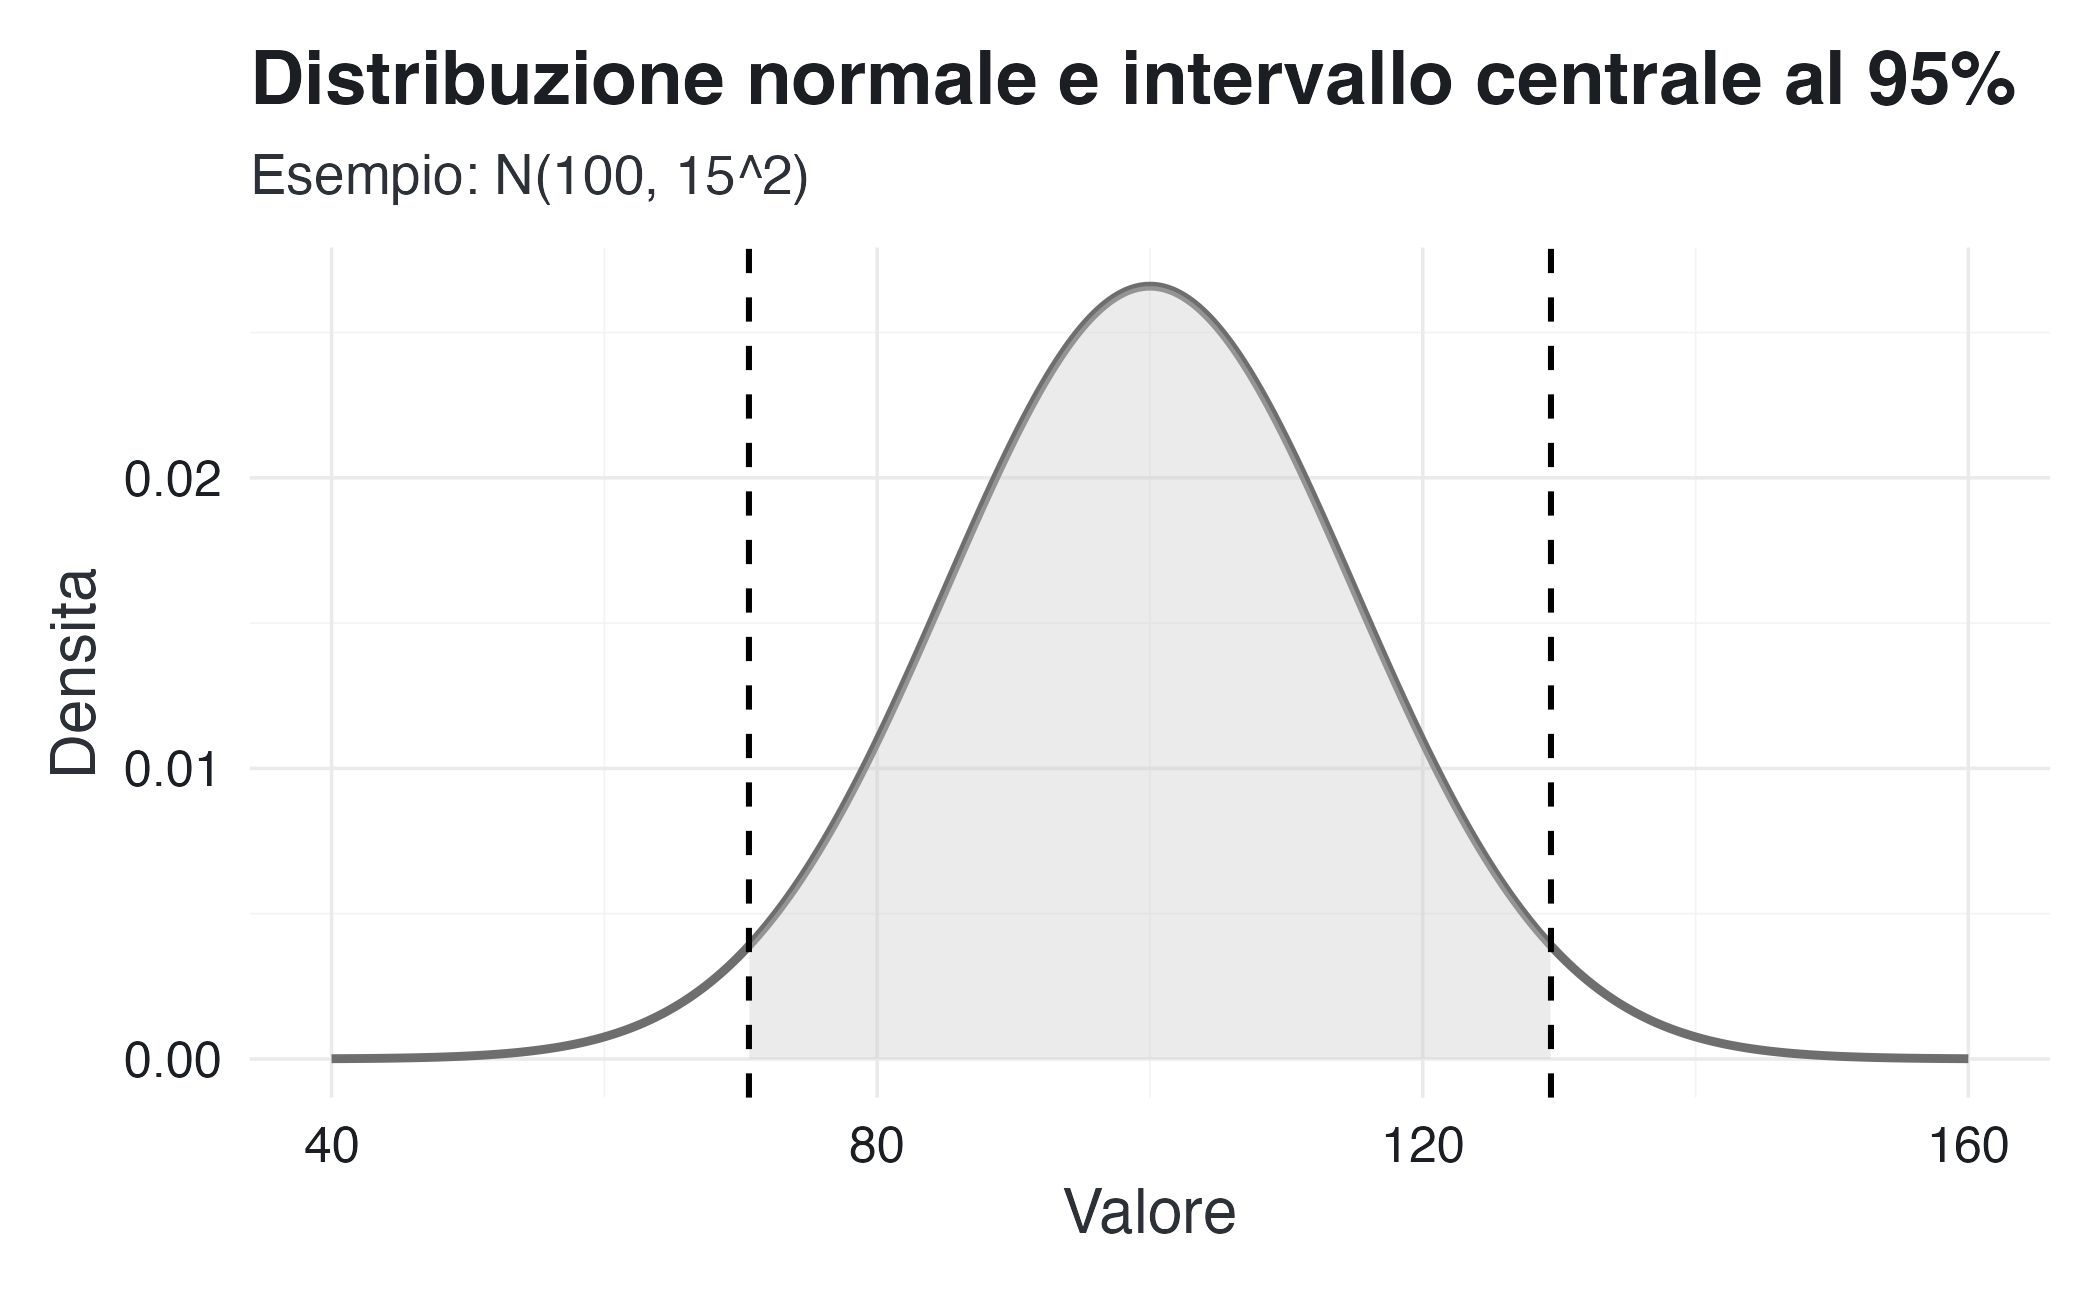
\includegraphics[width=0.85\linewidth,height=\textheight,keepaspectratio]{chapters/probability/12_cont_rv_distr_files/figure-pdf/unnamed-chunk-5-1.png}
\end{center}

\subsection{Quando la normale non e
appropriata}\label{quando-la-normale-non-e-appropriata}

La normale ha supporto su tutta la retta reale. Questo può essere
problematico per variabili che sono vincolate:

\begin{itemize}
\tightlist
\item
  tempi di risposta e durate, che sono sempre positivi e spesso
  asimmetrici;
\item
  conteggi di errori o sintomi, che sono discreti;
\item
  proporzioni, che sono limitate tra 0 e 1;
\item
  scale Likert con pochi livelli, che sono ordinali e limitate.
\end{itemize}

\begin{tcolorbox}[enhanced jigsaw, arc=.35mm, bottomrule=.15mm, bottomtitle=1mm, breakable, colback=white, colbacktitle=quarto-callout-warning-color!10!white, colframe=quarto-callout-warning-color-frame, coltitle=black, left=2mm, leftrule=.75mm, opacityback=0, opacitybacktitle=0.6, rightrule=.15mm, title=\textcolor{quarto-callout-warning-color}{\faExclamationTriangle}\hspace{0.5em}{Non normalizzare tutto}, titlerule=0mm, toprule=.15mm, toptitle=1mm]

La normale è comoda, ma non deve diventare una scelta automatica. Una
buona modellazione parte dalla natura del dato: supporto, simmetria,
presenza di code pesanti, vincoli inferiori o superiori, e significato
psicologico della variabile.

\end{tcolorbox}

\section{Distribuzione esponenziale}\label{sec-cont-exponential}

\subsection{Definizione}\label{definizione-6}

La distribuzione esponenziale modella il tempo di attesa fino al
verificarsi di un evento quando il tasso di occorrenza è costante nel
tempo.

\begin{definition}[]\protect\hypertarget{def-exponential}{}\label{def-exponential}

Una variabile casuale \(T\) segue una distribuzione esponenziale con
tasso \(\lambda > 0\) se

\[
T \sim \mathrm{Exp}(\lambda),
\qquad
f(t) = \lambda e^{-\lambda t}, \quad t \geq 0.
\]

Le proprietà principali sono:

\[
\mathbb{E}(T)=\frac{1}{\lambda},
\qquad
\mathbb{V}(T)=\frac{1}{\lambda^2}.
\]

\end{definition}

Il parametro \(\lambda\) è un \textbf{tasso}: eventi attesi per unità di
tempo. Il suo inverso, \(1/\lambda\), è il tempo medio di attesa.

\subsection{Assenza di memoria}\label{assenza-di-memoria}

La caratteristica distintiva della distribuzione esponenziale è la
proprieta di \textbf{assenza di memoria}:

\[
P(T > s+t \mid T > s) = P(T > t).
\]

In altre parole: aver già atteso fino a \(s\) non modifica la
distribuzione dell'attesa residua. È una proprietà molto restrittiva;
l'esponenziale è dunque appropriata solo quando il tasso costante è
un'assunzione plausibile.

\subsection{Esempio: tempo di attesa}\label{esempio-tempo-di-attesa}

Supponiamo che il tempo medio di attesa per un evento sia 4 giorni.
Allora \(\lambda = 1/4 = 0.25\).

\begin{Shaded}
\begin{Highlighting}[]
\NormalTok{lambda }\OtherTok{\textless{}{-}} \FloatTok{0.25}

\CommentTok{\# Probabilita di attendere al massimo 1.5 giorni.}
\FunctionTok{pexp}\NormalTok{(}\FloatTok{1.5}\NormalTok{, }\AttributeTok{rate =}\NormalTok{ lambda)}
\CommentTok{\#\textgreater{} [1] 0.313}

\CommentTok{\# Probabilita di attendere tra 1 e 6 giorni.}
\FunctionTok{pexp}\NormalTok{(}\DecValTok{6}\NormalTok{, }\AttributeTok{rate =}\NormalTok{ lambda) }\SpecialCharTok{{-}} \FunctionTok{pexp}\NormalTok{(}\DecValTok{1}\NormalTok{, }\AttributeTok{rate =}\NormalTok{ lambda)}
\CommentTok{\#\textgreater{} [1] 0.556}
\end{Highlighting}
\end{Shaded}

\begin{Shaded}
\begin{Highlighting}[]
\NormalTok{x }\OtherTok{\textless{}{-}} \FunctionTok{seq}\NormalTok{(}\DecValTok{0}\NormalTok{, }\DecValTok{20}\NormalTok{, }\AttributeTok{length.out =} \DecValTok{500}\NormalTok{)}
\NormalTok{df\_exp }\OtherTok{\textless{}{-}} \FunctionTok{data.frame}\NormalTok{(}
  \AttributeTok{x =}\NormalTok{ x,}
  \AttributeTok{densita =} \FunctionTok{dexp}\NormalTok{(x, }\AttributeTok{rate =}\NormalTok{ lambda),}
  \AttributeTok{area =}\NormalTok{ x }\SpecialCharTok{\textgreater{}=} \DecValTok{1} \SpecialCharTok{\&}\NormalTok{ x }\SpecialCharTok{\textless{}=} \DecValTok{6}
\NormalTok{)}

\FunctionTok{ggplot}\NormalTok{(df\_exp, }\FunctionTok{aes}\NormalTok{(}\AttributeTok{x =}\NormalTok{ x, }\AttributeTok{y =}\NormalTok{ densita)) }\SpecialCharTok{+}
  \FunctionTok{geom\_line}\NormalTok{(}\AttributeTok{linewidth =} \DecValTok{1}\NormalTok{) }\SpecialCharTok{+}
  \FunctionTok{geom\_area}\NormalTok{(}\AttributeTok{data =} \FunctionTok{subset}\NormalTok{(df\_exp, area), }\AttributeTok{alpha =} \FloatTok{0.4}\NormalTok{) }\SpecialCharTok{+}
  \FunctionTok{labs}\NormalTok{(}
    \AttributeTok{title =} \StringTok{"Distribuzione esponenziale"}\NormalTok{,}
    \AttributeTok{subtitle =} \StringTok{"Area evidenziata: P(1 \textless{}= T \textless{}= 6)"}\NormalTok{,}
    \AttributeTok{x =} \StringTok{"Tempo di attesa"}\NormalTok{,}
    \AttributeTok{y =} \StringTok{"Densita"}
\NormalTok{  )}
\end{Highlighting}
\end{Shaded}

\begin{center}
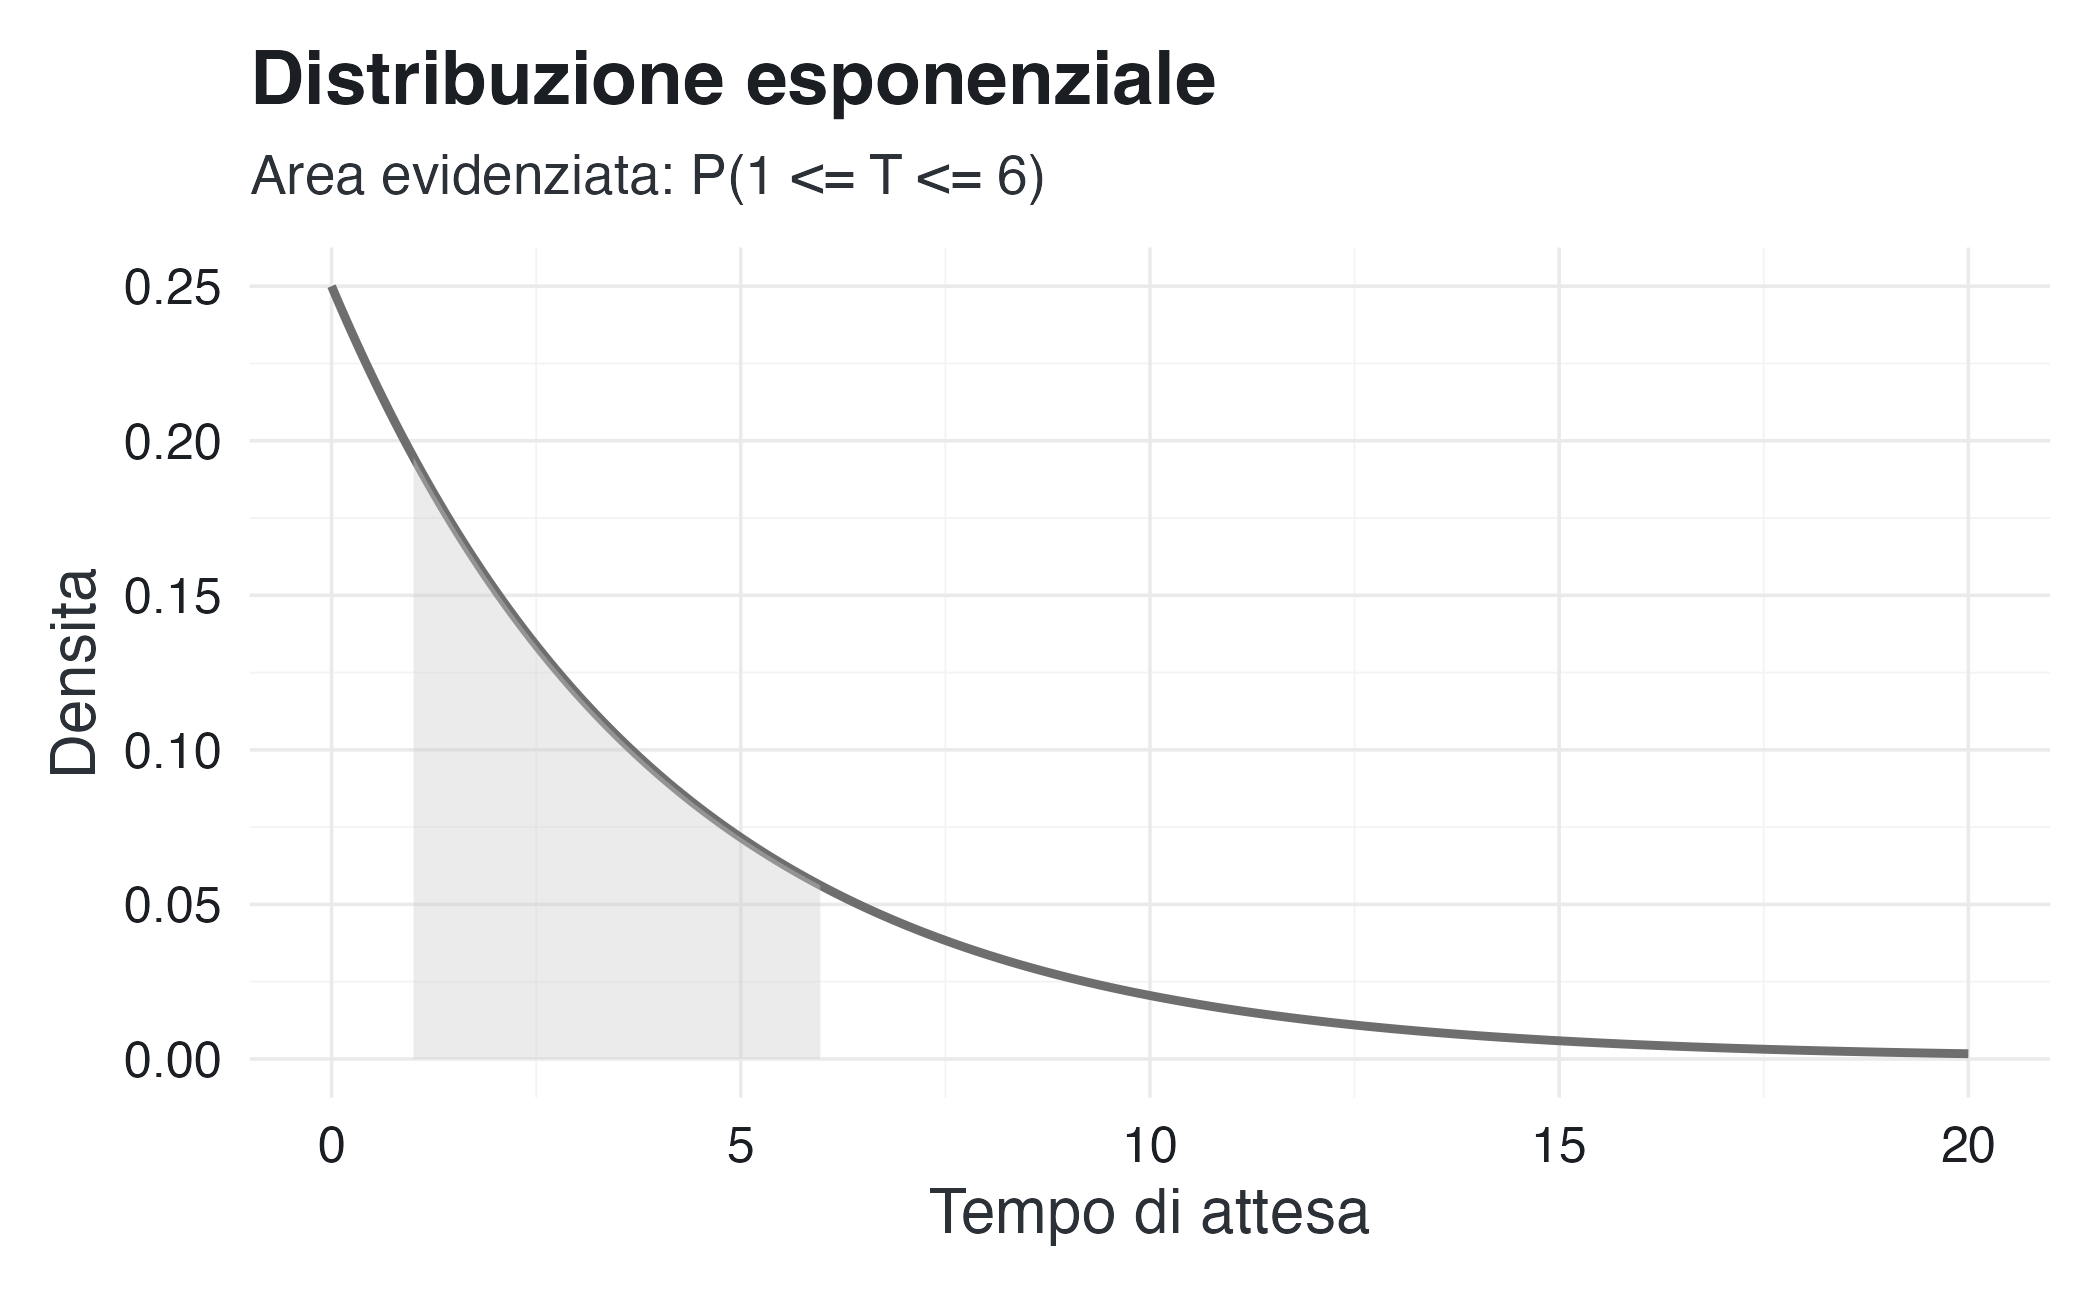
\includegraphics[width=0.85\linewidth,height=\textheight,keepaspectratio]{chapters/probability/12_cont_rv_distr_files/figure-pdf/unnamed-chunk-7-1.png}
\end{center}

\begin{tcolorbox}[enhanced jigsaw, arc=.35mm, bottomrule=.15mm, bottomtitle=1mm, breakable, colback=white, colbacktitle=quarto-callout-note-color!10!white, colframe=quarto-callout-note-color-frame, coltitle=black, left=2mm, leftrule=.75mm, opacityback=0, opacitybacktitle=0.6, rightrule=.15mm, title=\textcolor{quarto-callout-note-color}{\faInfo}\hspace{0.5em}{Applicazioni psicologiche}, titlerule=0mm, toprule=.15mm, toptitle=1mm]

L'esponenziale può essere utile per modellare le durate o i tempi tra
gli eventi quando il rischio istantaneo è approssimativamente costante,
ad esempio il tempo necessario per distrarsi, l'intervallo tra i
comportamenti osservabili o il tempo necessario perché si verifichi un
evento in un compito sperimentale.

Per i tempi di reazione, tuttavia, l'esponenziale è spesso troppo
semplice: distribuzioni come la log-normale, la gamma o l'ex-Gaussiana
possono essere più realistiche.

\end{tcolorbox}

\section{Distribuzione gamma}\label{sec-cont-gamma}

\subsection{Definizione}\label{definizione-7}

La distribuzione gamma è una famiglia flessibile per le variabili
positive. Può essere utilizzata per modellare tempi, durate, quantità
strettamente positive, tassi e precisioni.

In R useremo la parametrizzazione \textbf{shape-rate}.

\begin{definition}[]\protect\hypertarget{def-gamma}{}\label{def-gamma}

Una variabile casuale \(X\) segue una distribuzione gamma con parametri
\(\alpha > 0\) e \(\beta > 0\) se

\[
X \sim \mathrm{Gamma}(\alpha,\beta),
\] con densità

\[
f(x) = \frac{\beta^\alpha}{\Gamma(\alpha)} x^{\alpha-1} e^{-\beta x},
\qquad x > 0.
\]

Le sue proprietà principali sono:

\[
\mathbb{E}(X)=\frac{\alpha}{\beta},
\qquad
\mathbb{V}(X)=\frac{\alpha}{\beta^2}.
\]

\end{definition}

Il parametro \(\alpha\) controlla la forma della distribuzione, mentre
il parametro \(\beta\) controlla il tasso di decadimento. In R si usa
\texttt{dgamma(x,\ shape\ =\ alpha,\ rate\ =\ beta)}.

\begin{tcolorbox}[enhanced jigsaw, arc=.35mm, bottomrule=.15mm, bottomtitle=1mm, breakable, colback=white, colbacktitle=quarto-callout-warning-color!10!white, colframe=quarto-callout-warning-color-frame, coltitle=black, left=2mm, leftrule=.75mm, opacityback=0, opacitybacktitle=0.6, rightrule=.15mm, title=\textcolor{quarto-callout-warning-color}{\faExclamationTriangle}\hspace{0.5em}{Rate e scale}, titlerule=0mm, toprule=.15mm, toptitle=1mm]

Spesso, la gamma è parametrizzata anche con un parametro di scala
\(\theta = 1/\beta\). In R, l'argomento \texttt{rate} usa \(\beta\),
mentre l'argomento \texttt{scale} usa \(1/\beta\). Prima di utilizzare R
è necessario verificare la parametrizzazione.

\end{tcolorbox}

\subsection{Relazione con
l'esponenziale}\label{relazione-con-lesponenziale}

L'esponenziale è un caso particolare della gamma:

\[
\mathrm{Exp}(\lambda) = \mathrm{Gamma}(1,\lambda).
\]

In un processo a tasso costante, la gamma esprime il tempo necessario ad
accumulare più eventi. Se \(\alpha\) è intero, la gamma con parametro di
forma \(\alpha\) descrive l'attesa fino al verificarsi di \(\alpha\)
eventi.

\subsection{Ruolo bayesiano}\label{ruolo-bayesiano}

Nel percorso bayesiano, la gamma è importante per parametri positivi:

\begin{itemize}
\tightlist
\item
  come prior per un tasso \(\lambda > 0\);
\item
  come prior per una precisione \(\tau = 1/\sigma^2\);
\item
  come modello per durate positive e asimmetriche.
\end{itemize}

La distribuzione gamma è la coniugata naturale del tasso (\lambda) della
Poisson. Se nel capitolo precedente abbiamo scritto

\[
Y_i \mid \lambda \sim \mathrm{Poisson}(\lambda),
\]

allora una prior gamma su \(\lambda\) genera una posterior ancora gamma.
Tornerà utile quando affronteremo più esplicitamente l'aggiornamento
bayesiano.

\subsection{Flessibilità della forma}\label{flessibilituxe0-della-forma}

\begin{Shaded}
\begin{Highlighting}[]
\NormalTok{x }\OtherTok{\textless{}{-}} \FunctionTok{seq}\NormalTok{(}\DecValTok{0}\NormalTok{, }\DecValTok{10}\NormalTok{, }\AttributeTok{length.out =} \DecValTok{500}\NormalTok{)}
\NormalTok{params\_gamma }\OtherTok{\textless{}{-}} \FunctionTok{data.frame}\NormalTok{(}
  \AttributeTok{alpha =} \FunctionTok{c}\NormalTok{(}\DecValTok{1}\NormalTok{, }\DecValTok{2}\NormalTok{, }\DecValTok{4}\NormalTok{, }\DecValTok{9}\NormalTok{),}
  \AttributeTok{beta =} \FunctionTok{c}\NormalTok{(}\DecValTok{1}\NormalTok{, }\DecValTok{1}\NormalTok{, }\DecValTok{1}\NormalTok{, }\DecValTok{2}\NormalTok{)}
\NormalTok{)}

\NormalTok{df\_gamma }\OtherTok{\textless{}{-}} \FunctionTok{do.call}\NormalTok{(rbind, }\FunctionTok{lapply}\NormalTok{(}\FunctionTok{seq\_len}\NormalTok{(}\FunctionTok{nrow}\NormalTok{(params\_gamma)), }\ControlFlowTok{function}\NormalTok{(i) \{}
\NormalTok{  alpha }\OtherTok{\textless{}{-}}\NormalTok{ params\_gamma}\SpecialCharTok{$}\NormalTok{alpha[i]}
\NormalTok{  beta }\OtherTok{\textless{}{-}}\NormalTok{ params\_gamma}\SpecialCharTok{$}\NormalTok{beta[i]}
  \FunctionTok{data.frame}\NormalTok{(}
    \AttributeTok{x =}\NormalTok{ x,}
    \AttributeTok{densita =} \FunctionTok{dgamma}\NormalTok{(x, }\AttributeTok{shape =}\NormalTok{ alpha, }\AttributeTok{rate =}\NormalTok{ beta),}
    \AttributeTok{distribuzione =} \FunctionTok{paste0}\NormalTok{(}\StringTok{"Gamma("}\NormalTok{, alpha, }\StringTok{", "}\NormalTok{, beta, }\StringTok{")"}\NormalTok{)}
\NormalTok{  )}
\NormalTok{\}))}

\FunctionTok{ggplot}\NormalTok{(df\_gamma, }\FunctionTok{aes}\NormalTok{(}\AttributeTok{x =}\NormalTok{ x, }\AttributeTok{y =}\NormalTok{ densita, }\AttributeTok{color =}\NormalTok{ distribuzione)) }\SpecialCharTok{+}
  \FunctionTok{geom\_line}\NormalTok{(}\AttributeTok{linewidth =} \DecValTok{1}\NormalTok{) }\SpecialCharTok{+}
  \FunctionTok{labs}\NormalTok{(}
    \AttributeTok{title =} \StringTok{"Flessibilita della distribuzione gamma"}\NormalTok{,}
    \AttributeTok{x =} \StringTok{"x"}\NormalTok{,}
    \AttributeTok{y =} \StringTok{"Densita"}\NormalTok{,}
    \AttributeTok{color =} \StringTok{"Distribuzione"}
\NormalTok{  )}
\end{Highlighting}
\end{Shaded}

\begin{center}
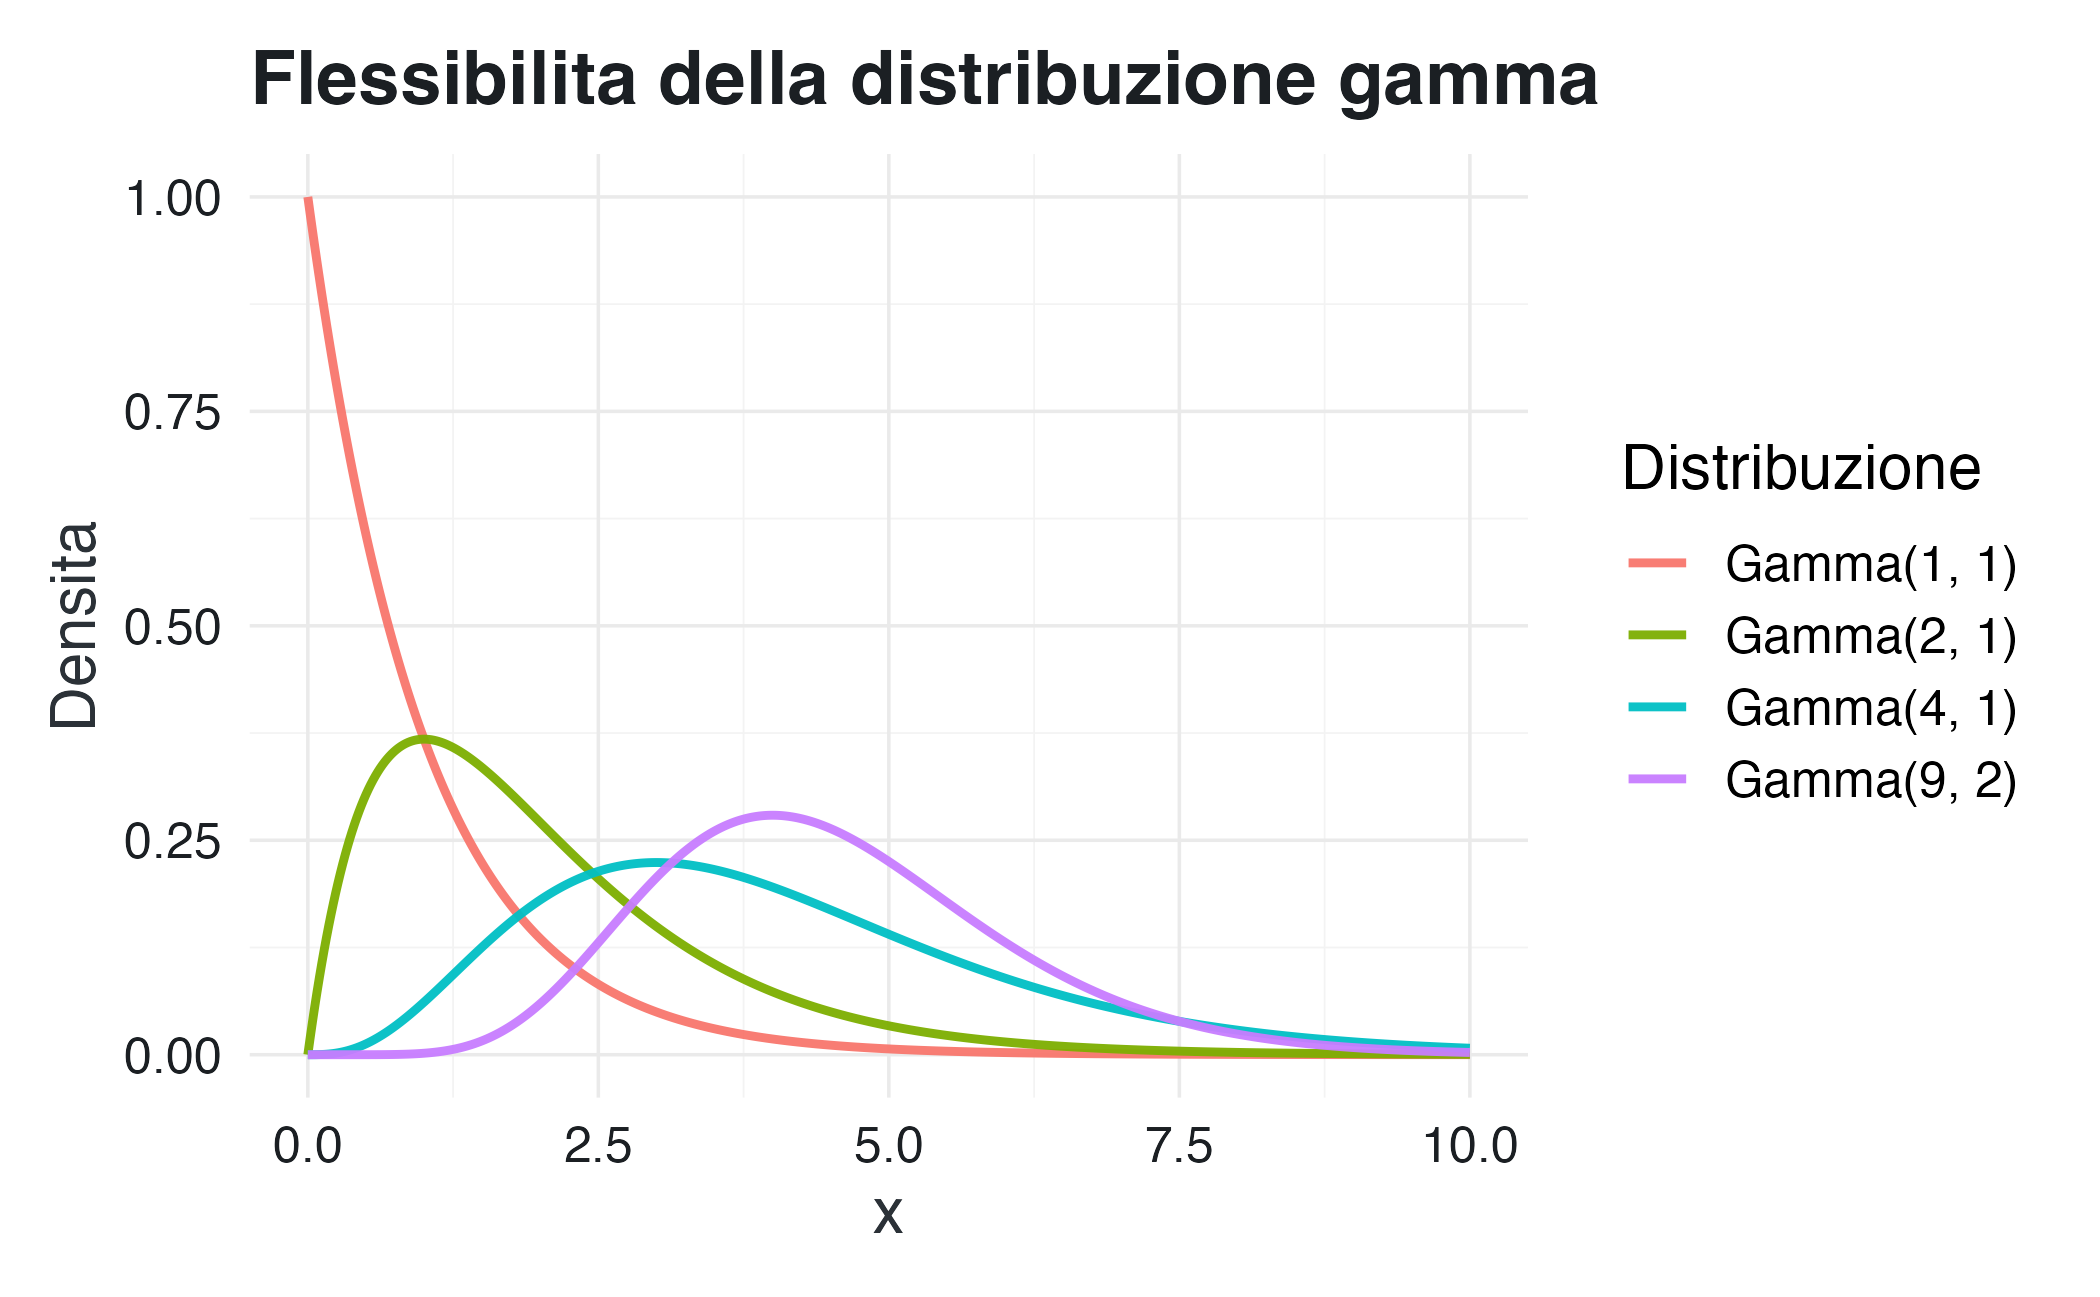
\includegraphics[width=0.85\linewidth,height=\textheight,keepaspectratio]{chapters/probability/12_cont_rv_distr_files/figure-pdf/unnamed-chunk-8-1.png}
\end{center}

\begin{tcolorbox}[enhanced jigsaw, arc=.35mm, bottomrule=.15mm, bottomtitle=1mm, breakable, colback=white, colbacktitle=quarto-callout-tip-color!10!white, colframe=quarto-callout-tip-color-frame, coltitle=black, left=2mm, leftrule=.75mm, opacityback=0, opacitybacktitle=0.6, rightrule=.15mm, title=\textcolor{quarto-callout-tip-color}{\faLightbulb}\hspace{0.5em}{Anticipazione: aggiornamento Gamma-Poisson}, titlerule=0mm, toprule=.15mm, toptitle=1mm]

Se \(\lambda \sim \mathrm{Gamma}(\alpha_0,\beta_0)\) e osserviamo
conteggi Poisson indipendenti \(y_1,\ldots,y_n\), allora

\[
\lambda \mid y \sim
\mathrm{Gamma}\left(\alpha_0 + \sum_{i=1}^n y_i,\; \beta_0+n\right).
\]

Questa formula non è ancora il tema centrale del capitolo, ma serve solo
a mostrare perché la gamma è una distribuzione così utile nel
vocabolario bayesiano.

\end{tcolorbox}

\section{Distribuzione beta}\label{sec-cont-beta}

\subsection{Definizione}\label{definizione-8}

La distribuzione beta è definita sull'intervallo \((0,1)\). Per questo
motivo, è la scelta naturale per rappresentare l'incertezza su
probabilità, proporzioni e parametri vincolati tra 0 e 1.

\begin{definition}[]\protect\hypertarget{def-beta}{}\label{def-beta}

Una variabile casuale \(\theta\) segue una distribuzione beta con
parametri \(\alpha > 0\) e \(\beta > 0\) se

\[
\theta \sim \mathrm{Beta}(\alpha,\beta),
\] con densità

\[
f(\theta) = \frac{\theta^{\alpha-1}(1-\theta)^{\beta-1}}{B(\alpha,\beta)},
\qquad 0 < \theta < 1.
\]

Le proprietà principali sono:

\[
\mathbb{E}(\theta)=\frac{\alpha}{\alpha+\beta},
\]

\[
\mathbb{V}(\theta)=
\frac{\alpha\beta}{(\alpha+\beta)^2(\alpha+\beta+1)}.
\]

\end{definition}

\subsection{Interpretazione dei
parametri}\label{interpretazione-dei-parametri-1}

La beta è particolarmente intuitiva in un contesto bayesiano. I
parametri possono essere letti come una forma di informazione
preliminare:

\begin{itemize}
\tightlist
\item
  \(\alpha\) è collegato alla quantità di evidenza a favore dell'evento;
\item
  \(\beta\) è collegato alla quantità di evidenza contro l'evento;
\item
  \(\alpha + \beta\) rappresenta la forza complessiva della
  distribuzione.
\end{itemize}

Una distribuzione \(\mathrm{Beta}(1,1)\) è uniforme su \((0,1)\). Una
\(\mathrm{Beta}(20,10)\) concentra la massa attorno a valori più alti,
come se l'informazione preliminare suggerisse più successi che
insuccessi.

\begin{tcolorbox}[enhanced jigsaw, arc=.35mm, bottomrule=.15mm, bottomtitle=1mm, breakable, colback=white, colbacktitle=quarto-callout-note-color!10!white, colframe=quarto-callout-note-color-frame, coltitle=black, left=2mm, leftrule=.75mm, opacityback=0, opacitybacktitle=0.6, rightrule=.15mm, title=\textcolor{quarto-callout-note-color}{\faInfo}\hspace{0.5em}{Pseudo-osservazioni: una convenzione utile}, titlerule=0mm, toprule=.15mm, toptitle=1mm]

Spesso, si interpreta \(\alpha-1\) come il numero di pseudo-successi e
\(\beta-1\) come il numero di pseudo-insuccessi. In altri contesti,
invece, si usano \(\alpha\) e \(\beta\) come conteggi effettivi.
L'importante è non confondere la metafora con una regola universale: la
distribuzione beta rappresenta una distribuzione di credenze, non
necessariamente un vero campione precedente.

\end{tcolorbox}

\subsection{Ruolo bayesiano}\label{ruolo-bayesiano-1}

La distribuzione beta è la prior coniugata naturale per il parametro di
una distribuzione di Bernoulli o binomiale:

\[
Y \mid \theta \sim \mathrm{Binomiale}(n,\theta),
\qquad
\theta \sim \mathrm{Beta}(\alpha,\beta).
\]

Dopo aver osservato \(y\) successi su \(n\) prove, la distribuzione a
posteriori è:

\[
\theta \mid y \sim \mathrm{Beta}(\alpha+y,\beta+n-y).
\]

Nel capitolo 13 useremo proprio questo tipo di modello per collegare la
proporzione campionaria, l'errore standard e l'informazione nei dati.

\subsection{Forme possibili}\label{forme-possibili}

\begin{Shaded}
\begin{Highlighting}[]
\NormalTok{x }\OtherTok{\textless{}{-}} \FunctionTok{seq}\NormalTok{(}\FloatTok{0.001}\NormalTok{, }\FloatTok{0.999}\NormalTok{, }\AttributeTok{length.out =} \DecValTok{500}\NormalTok{)}
\NormalTok{params\_beta }\OtherTok{\textless{}{-}} \FunctionTok{data.frame}\NormalTok{(}
  \AttributeTok{alpha =} \FunctionTok{c}\NormalTok{(}\FloatTok{0.5}\NormalTok{, }\DecValTok{1}\NormalTok{, }\DecValTok{2}\NormalTok{, }\DecValTok{2}\NormalTok{, }\DecValTok{5}\NormalTok{, }\DecValTok{20}\NormalTok{),}
  \AttributeTok{beta =} \FunctionTok{c}\NormalTok{(}\FloatTok{0.5}\NormalTok{, }\DecValTok{1}\NormalTok{, }\DecValTok{2}\NormalTok{, }\DecValTok{5}\NormalTok{, }\DecValTok{2}\NormalTok{, }\DecValTok{10}\NormalTok{)}
\NormalTok{)}

\NormalTok{df\_beta }\OtherTok{\textless{}{-}} \FunctionTok{do.call}\NormalTok{(rbind, }\FunctionTok{lapply}\NormalTok{(}\FunctionTok{seq\_len}\NormalTok{(}\FunctionTok{nrow}\NormalTok{(params\_beta)), }\ControlFlowTok{function}\NormalTok{(i) \{}
\NormalTok{  alpha }\OtherTok{\textless{}{-}}\NormalTok{ params\_beta}\SpecialCharTok{$}\NormalTok{alpha[i]}
\NormalTok{  beta }\OtherTok{\textless{}{-}}\NormalTok{ params\_beta}\SpecialCharTok{$}\NormalTok{beta[i]}
  \FunctionTok{data.frame}\NormalTok{(}
    \AttributeTok{x =}\NormalTok{ x,}
    \AttributeTok{densita =} \FunctionTok{dbeta}\NormalTok{(x, }\AttributeTok{shape1 =}\NormalTok{ alpha, }\AttributeTok{shape2 =}\NormalTok{ beta),}
    \AttributeTok{distribuzione =} \FunctionTok{paste0}\NormalTok{(}\StringTok{"Beta("}\NormalTok{, alpha, }\StringTok{", "}\NormalTok{, beta, }\StringTok{")"}\NormalTok{)}
\NormalTok{  )}
\NormalTok{\}))}

\FunctionTok{ggplot}\NormalTok{(df\_beta, }\FunctionTok{aes}\NormalTok{(}\AttributeTok{x =}\NormalTok{ x, }\AttributeTok{y =}\NormalTok{ densita, }\AttributeTok{color =}\NormalTok{ distribuzione)) }\SpecialCharTok{+}
  \FunctionTok{geom\_line}\NormalTok{(}\AttributeTok{linewidth =} \DecValTok{1}\NormalTok{) }\SpecialCharTok{+}
  \FunctionTok{labs}\NormalTok{(}
    \AttributeTok{title =} \StringTok{"Flessibilita della distribuzione beta"}\NormalTok{,}
    \AttributeTok{subtitle =} \StringTok{"La beta puo rappresentare ignoranza, preferenze moderate o credenze concentrate"}\NormalTok{,}
    \AttributeTok{x =} \FunctionTok{expression}\NormalTok{(theta),}
    \AttributeTok{y =} \StringTok{"Densita"}\NormalTok{,}
    \AttributeTok{color =} \StringTok{"Distribuzione"}
\NormalTok{  )}
\end{Highlighting}
\end{Shaded}

\begin{center}
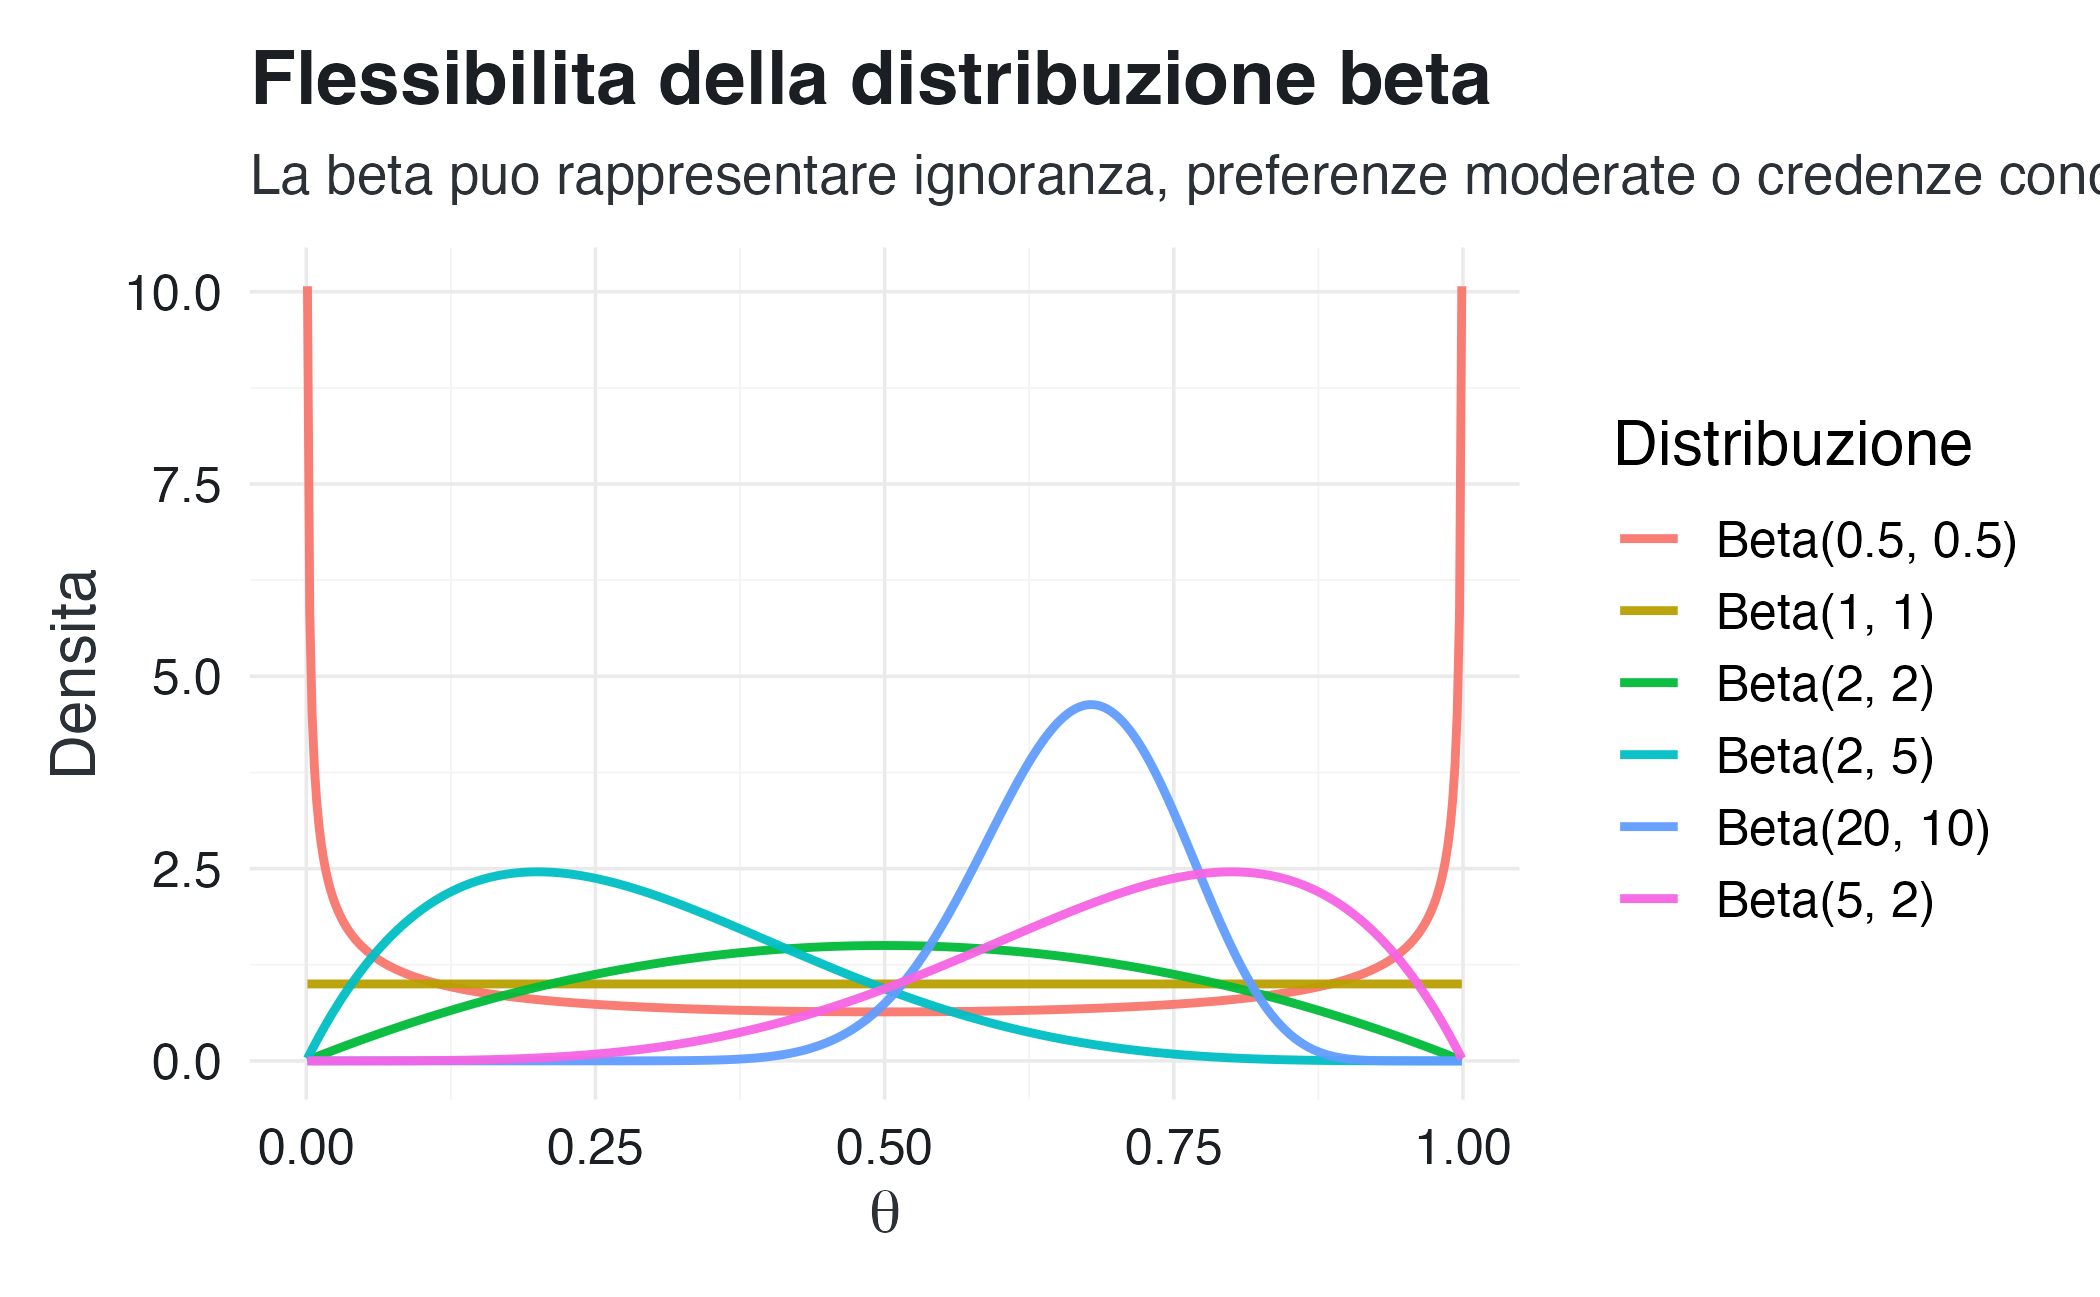
\includegraphics[width=0.85\linewidth,height=\textheight,keepaspectratio]{chapters/probability/12_cont_rv_distr_files/figure-pdf/unnamed-chunk-9-1.png}
\end{center}

\section{Distribuzione chi-quadrato}\label{sec-cont-chisq}

\subsection{Definizione}\label{definizione-9}

La distribuzione chi-quadrato nasce dalla somma di quadrati di variabili
normali standard indipendenti.

\begin{definition}[]\protect\hypertarget{def-chisq}{}\label{def-chisq}

Se

\[
Z_1,\ldots,Z_k \stackrel{iid}{\sim} \mathcal{N}(0,1),
\] allora \[
X = Z_1^2 + \cdots + Z_k^2 \sim \chi^2_k.
\]

Il parametro \(k\) è il numero di gradi di libertà. Le proprietà
principali sono:

\[
\mathbb{E}(X)=k,
\qquad
\mathbb{V}(X)=2k.
\]

\end{definition}

\subsection{Interpretazione}\label{interpretazione-1}

La chi-quadrato misura una dispersione quadratica: somma le deviazioni
standardizzate, le eleva al quadrato e quindi considera la grandezza
complessiva dello scostamento, a prescindere dal segno.

Si tratta di un caso particolare della funzione gamma:

\[
\chi^2_k = \mathrm{Gamma}\left(\frac{k}{2},\frac{1}{2}\right)
\] nella parametrizzazione shape-rate.

\subsection{Ruolo bayesiano}\label{ruolo-bayesiano-2}

La chi-quadrato è importante perché compare nella teoria della varianza
campionaria e, indirettamente, nei modelli normali con varianza
sconosciuta. Nelle formulazioni bayesiane moderne si lavora spesso con
distribuzioni gamma o inverse-gamma per varianze e precisioni, ma la
chi-quadrato rimane un ponte concettuale utile.

\begin{Shaded}
\begin{Highlighting}[]
\NormalTok{x }\OtherTok{\textless{}{-}} \FunctionTok{seq}\NormalTok{(}\DecValTok{0}\NormalTok{, }\DecValTok{40}\NormalTok{, }\AttributeTok{length.out =} \DecValTok{500}\NormalTok{)}
\NormalTok{df\_chisq }\OtherTok{\textless{}{-}} \FunctionTok{data.frame}\NormalTok{(}
  \AttributeTok{x =} \FunctionTok{rep}\NormalTok{(x, }\DecValTok{4}\NormalTok{),}
  \AttributeTok{densita =} \FunctionTok{c}\NormalTok{(}\FunctionTok{dchisq}\NormalTok{(x, }\AttributeTok{df =} \DecValTok{2}\NormalTok{), }\FunctionTok{dchisq}\NormalTok{(x, }\AttributeTok{df =} \DecValTok{4}\NormalTok{),}
              \FunctionTok{dchisq}\NormalTok{(x, }\AttributeTok{df =} \DecValTok{8}\NormalTok{), }\FunctionTok{dchisq}\NormalTok{(x, }\AttributeTok{df =} \DecValTok{16}\NormalTok{)),}
  \AttributeTok{df =} \FunctionTok{rep}\NormalTok{(}\FunctionTok{c}\NormalTok{(}\StringTok{"2"}\NormalTok{, }\StringTok{"4"}\NormalTok{, }\StringTok{"8"}\NormalTok{, }\StringTok{"16"}\NormalTok{), }\AttributeTok{each =} \FunctionTok{length}\NormalTok{(x))}
\NormalTok{)}

\FunctionTok{ggplot}\NormalTok{(df\_chisq, }\FunctionTok{aes}\NormalTok{(}\AttributeTok{x =}\NormalTok{ x, }\AttributeTok{y =}\NormalTok{ densita, }\AttributeTok{color =}\NormalTok{ df)) }\SpecialCharTok{+}
  \FunctionTok{geom\_line}\NormalTok{(}\AttributeTok{linewidth =} \DecValTok{1}\NormalTok{) }\SpecialCharTok{+}
  \FunctionTok{labs}\NormalTok{(}
    \AttributeTok{title =} \StringTok{"Distribuzione chi{-}quadrato"}\NormalTok{,}
    \AttributeTok{subtitle =} \StringTok{"All\textquotesingle{}aumentare dei gradi di liberta la distribuzione diventa meno asimmetrica"}\NormalTok{,}
    \AttributeTok{x =} \StringTok{"x"}\NormalTok{,}
    \AttributeTok{y =} \StringTok{"Densita"}\NormalTok{,}
    \AttributeTok{color =} \StringTok{"Gradi di liberta"}
\NormalTok{  )}
\end{Highlighting}
\end{Shaded}

\begin{center}
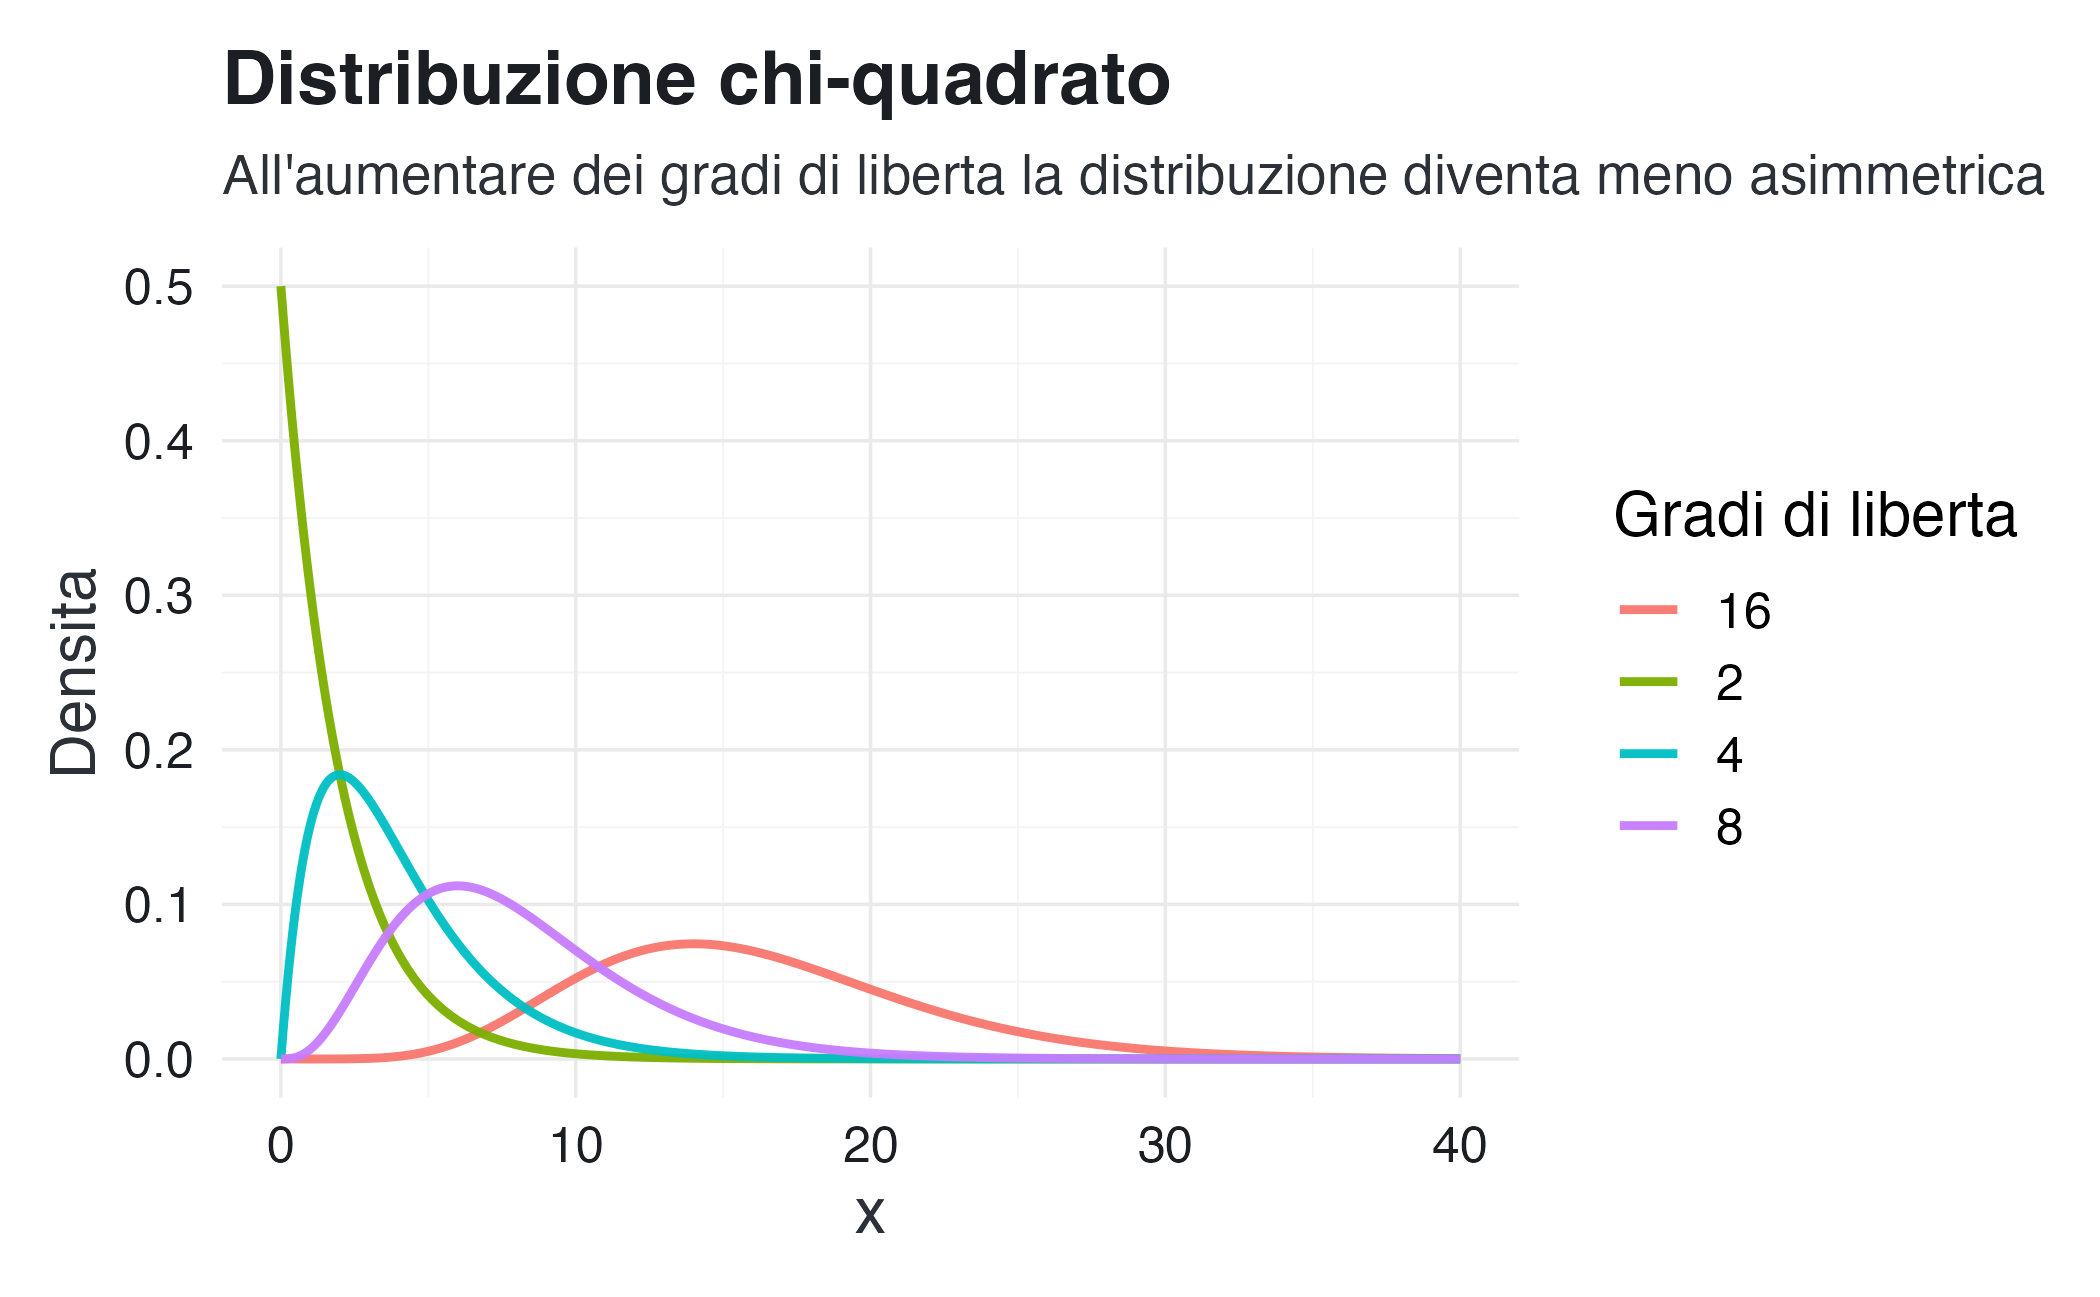
\includegraphics[width=0.85\linewidth,height=\textheight,keepaspectratio]{chapters/probability/12_cont_rv_distr_files/figure-pdf/unnamed-chunk-10-1.png}
\end{center}

\section{Distribuzione t di Student}\label{sec-cont-student-t}

\subsection{Definizione}\label{definizione-10}

La distribuzione \(t\) di Student emerge quando una variabile normale
viene standardizzata utilizzando una stima incerta della sua varianza.

\begin{definition}[]\protect\hypertarget{def-student-t}{}\label{def-student-t}

Se \(Z \sim \mathcal{N}(0,1)\), \(W \sim \chi^2_\nu\) e \(Z\) e \(W\)
sono indipendenti, allora

\[
T = \frac{Z}{\sqrt{W/\nu}} \sim t_\nu.
\]

Il parametro \(\nu\) rappresenta i gradi di libertà.

\end{definition}

\subsection{Interpretazione}\label{interpretazione-2}

La \(t\) assomiglia alla normale, ma ha \textbf{code più pesanti},
soprattutto quando \(\nu\) e piccolo. Ciò significa che assegna maggiore
plausibilità a valori lontani dal centro.

Quando \(\nu\) aumenta, la \(t\) tende alla distribuzione normale
standard.

\subsection{Ruolo bayesiano}\label{ruolo-bayesiano-3}

La \(t\) è utile in due modi:

\begin{enumerate}
\def\labelenumi{\arabic{enumi}.}
\tightlist
\item
  come modello o distribuzione predittiva quando la scala è incerta;
\item
  come prior debolmente informativa e robusta per parametri continui.
\end{enumerate}

Nel lavoro applicato, l'uso di una distribuzione \(t\) al posto di una
normale può ridurre la sensibilità del modello ai valori estremi.

\begin{Shaded}
\begin{Highlighting}[]
\NormalTok{x }\OtherTok{\textless{}{-}} \FunctionTok{seq}\NormalTok{(}\SpecialCharTok{{-}}\DecValTok{5}\NormalTok{, }\DecValTok{5}\NormalTok{, }\AttributeTok{length.out =} \DecValTok{500}\NormalTok{)}
\NormalTok{df\_t }\OtherTok{\textless{}{-}} \FunctionTok{data.frame}\NormalTok{(}
  \AttributeTok{x =} \FunctionTok{rep}\NormalTok{(x, }\DecValTok{4}\NormalTok{),}
  \AttributeTok{densita =} \FunctionTok{c}\NormalTok{(}\FunctionTok{dnorm}\NormalTok{(x), }\FunctionTok{dt}\NormalTok{(x, }\AttributeTok{df =} \DecValTok{1}\NormalTok{), }\FunctionTok{dt}\NormalTok{(x, }\AttributeTok{df =} \DecValTok{3}\NormalTok{), }\FunctionTok{dt}\NormalTok{(x, }\AttributeTok{df =} \DecValTok{10}\NormalTok{)),}
  \AttributeTok{distribuzione =} \FunctionTok{rep}\NormalTok{(}\FunctionTok{c}\NormalTok{(}\StringTok{"Normale"}\NormalTok{, }\StringTok{"t(1)"}\NormalTok{, }\StringTok{"t(3)"}\NormalTok{, }\StringTok{"t(10)"}\NormalTok{), }\AttributeTok{each =} \FunctionTok{length}\NormalTok{(x))}
\NormalTok{)}

\FunctionTok{ggplot}\NormalTok{(df\_t, }\FunctionTok{aes}\NormalTok{(}\AttributeTok{x =}\NormalTok{ x, }\AttributeTok{y =}\NormalTok{ densita, }\AttributeTok{color =}\NormalTok{ distribuzione)) }\SpecialCharTok{+}
  \FunctionTok{geom\_line}\NormalTok{(}\AttributeTok{linewidth =} \DecValTok{1}\NormalTok{) }\SpecialCharTok{+}
  \FunctionTok{labs}\NormalTok{(}
    \AttributeTok{title =} \StringTok{"Confronto tra normale e t di Student"}\NormalTok{,}
    \AttributeTok{subtitle =} \StringTok{"Con pochi gradi di liberta, la t ha code piu pesanti"}\NormalTok{,}
    \AttributeTok{x =} \StringTok{"x"}\NormalTok{,}
    \AttributeTok{y =} \StringTok{"Densita"}\NormalTok{,}
    \AttributeTok{color =} \StringTok{"Distribuzione"}
\NormalTok{  )}
\end{Highlighting}
\end{Shaded}

\begin{center}
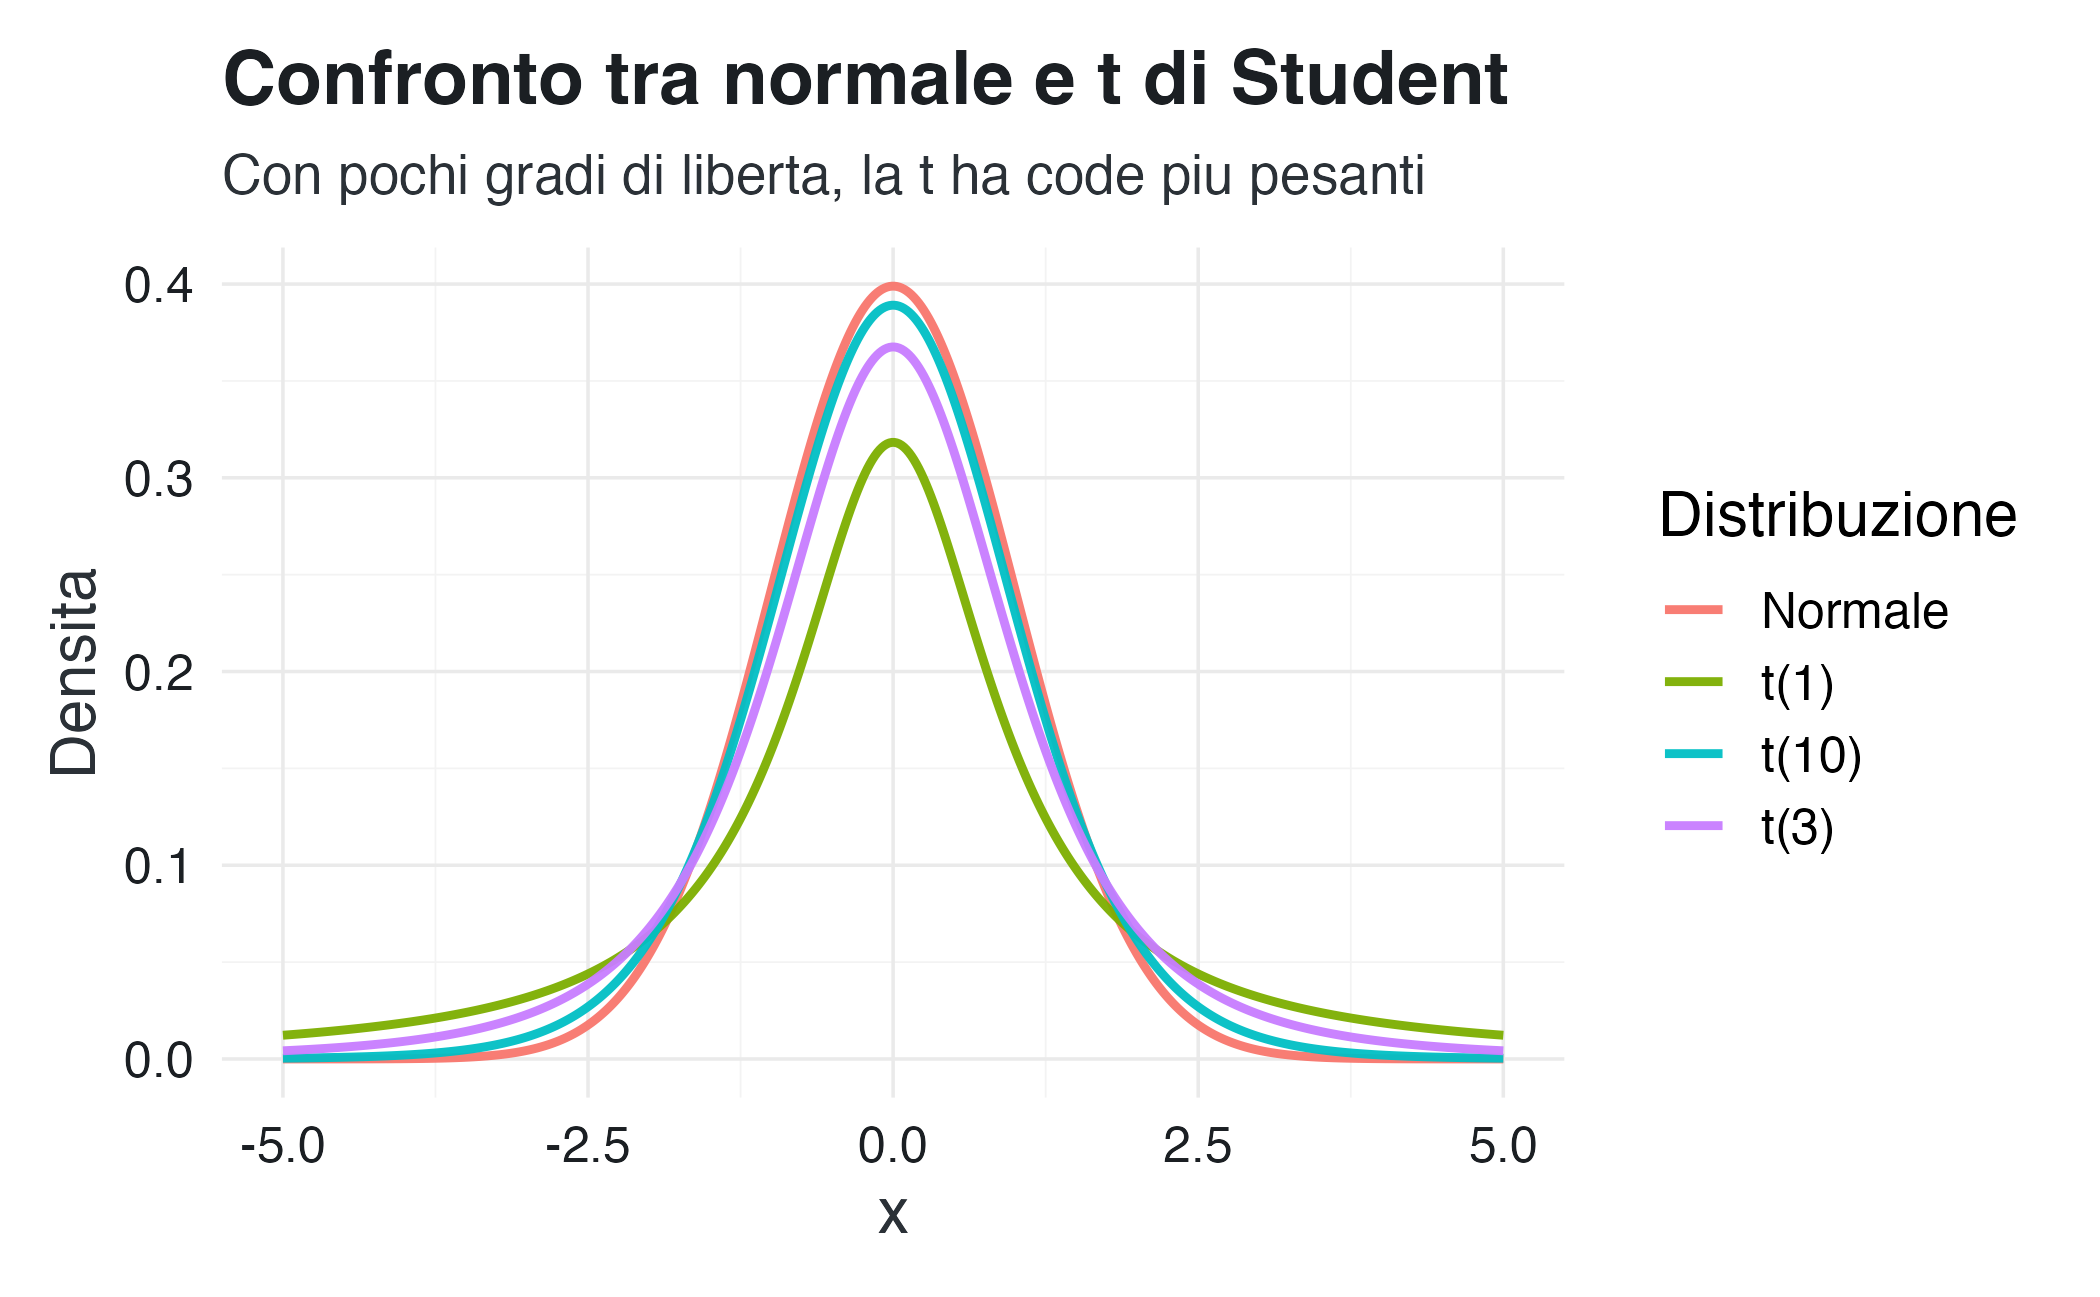
\includegraphics[width=0.85\linewidth,height=\textheight,keepaspectratio]{chapters/probability/12_cont_rv_distr_files/figure-pdf/unnamed-chunk-11-1.png}
\end{center}

\section{Distribuzione di Cauchy}\label{sec-cont-cauchy}

\subsection{Definizione}\label{definizione-11}

La distribuzione di Cauchy è un caso particolare della distribuzione
\(t\) con un solo grado di libertà.

\begin{definition}[]\protect\hypertarget{def-cauchy}{}\label{def-cauchy}

Una variabile casuale \(X\) segue una distribuzione di Cauchy con
parametro di posizione \(x_0\) e parametro di scala \(s>0\) se

\[
X \sim \mathrm{Cauchy}(x_0,s),
\] con densità \[
f(x)=\frac{1}{\pi s\left[1+\left(\frac{x-x_0}{s}\right)^2\right]}.
\]

\end{definition}

La distribuzione di Cauchy ha code molto pesanti e non possiede media e
varianza finite. Il parametro \(x_0\) indica una posizione centrale, ma
non è una media nel senso usuale.

\subsection{Ruolo bayesiano}\label{ruolo-bayesiano-4}

La distribuzione di Cauchy è spesso utilizzata come prior robusta e
debolmente informativa per i parametri di posizione o i coefficienti di
regressione. La sua versione troncata ai valori positivi, detta
\emph{half-Cauchy}, è usata come prior per i parametri di scala, ad
esempio le deviazioni standard nei modelli gerarchici.

\begin{tcolorbox}[enhanced jigsaw, arc=.35mm, bottomrule=.15mm, bottomtitle=1mm, breakable, colback=white, colbacktitle=quarto-callout-warning-color!10!white, colframe=quarto-callout-warning-color-frame, coltitle=black, left=2mm, leftrule=.75mm, opacityback=0, opacitybacktitle=0.6, rightrule=.15mm, title=\textcolor{quarto-callout-warning-color}{\faExclamationTriangle}\hspace{0.5em}{Code pesanti non significa assenza di assunzioni}, titlerule=0mm, toprule=.15mm, toptitle=1mm]

Una prior Cauchy lascia molto spazio ai valori estremi. Questo può
essere utile per la robustezza, ma può anche rendere l'inferenza
instabile se i dati sono pochi o il modello è debole. Una prior robusta
non sostituisce il ragionamento sostanziale sulla scala plausibile degli
effetti.

\end{tcolorbox}

\begin{Shaded}
\begin{Highlighting}[]
\NormalTok{x }\OtherTok{\textless{}{-}} \FunctionTok{seq}\NormalTok{(}\SpecialCharTok{{-}}\DecValTok{10}\NormalTok{, }\DecValTok{10}\NormalTok{, }\AttributeTok{length.out =} \DecValTok{800}\NormalTok{)}
\NormalTok{df\_cauchy }\OtherTok{\textless{}{-}} \FunctionTok{data.frame}\NormalTok{(}
  \AttributeTok{x =} \FunctionTok{rep}\NormalTok{(x, }\DecValTok{3}\NormalTok{),}
  \AttributeTok{densita =} \FunctionTok{c}\NormalTok{(}\FunctionTok{dnorm}\NormalTok{(x), }\FunctionTok{dt}\NormalTok{(x, }\AttributeTok{df =} \DecValTok{3}\NormalTok{), }\FunctionTok{dcauchy}\NormalTok{(x)),}
  \AttributeTok{distribuzione =} \FunctionTok{rep}\NormalTok{(}\FunctionTok{c}\NormalTok{(}\StringTok{"Normale(0,1)"}\NormalTok{, }\StringTok{"t(3)"}\NormalTok{, }\StringTok{"Cauchy(0,1)"}\NormalTok{), }\AttributeTok{each =} \FunctionTok{length}\NormalTok{(x))}
\NormalTok{)}

\FunctionTok{ggplot}\NormalTok{(df\_cauchy, }\FunctionTok{aes}\NormalTok{(}\AttributeTok{x =}\NormalTok{ x, }\AttributeTok{y =}\NormalTok{ densita, }\AttributeTok{color =}\NormalTok{ distribuzione)) }\SpecialCharTok{+}
  \FunctionTok{geom\_line}\NormalTok{(}\AttributeTok{linewidth =} \DecValTok{1}\NormalTok{) }\SpecialCharTok{+}
  \FunctionTok{labs}\NormalTok{(}
    \AttributeTok{title =} \StringTok{"Normale, t e Cauchy"}\NormalTok{,}
    \AttributeTok{subtitle =} \StringTok{"La Cauchy assegna molta piu massa alle code"}\NormalTok{,}
    \AttributeTok{x =} \StringTok{"x"}\NormalTok{,}
    \AttributeTok{y =} \StringTok{"Densita"}\NormalTok{,}
    \AttributeTok{color =} \StringTok{"Distribuzione"}
\NormalTok{  )}
\end{Highlighting}
\end{Shaded}

\begin{center}
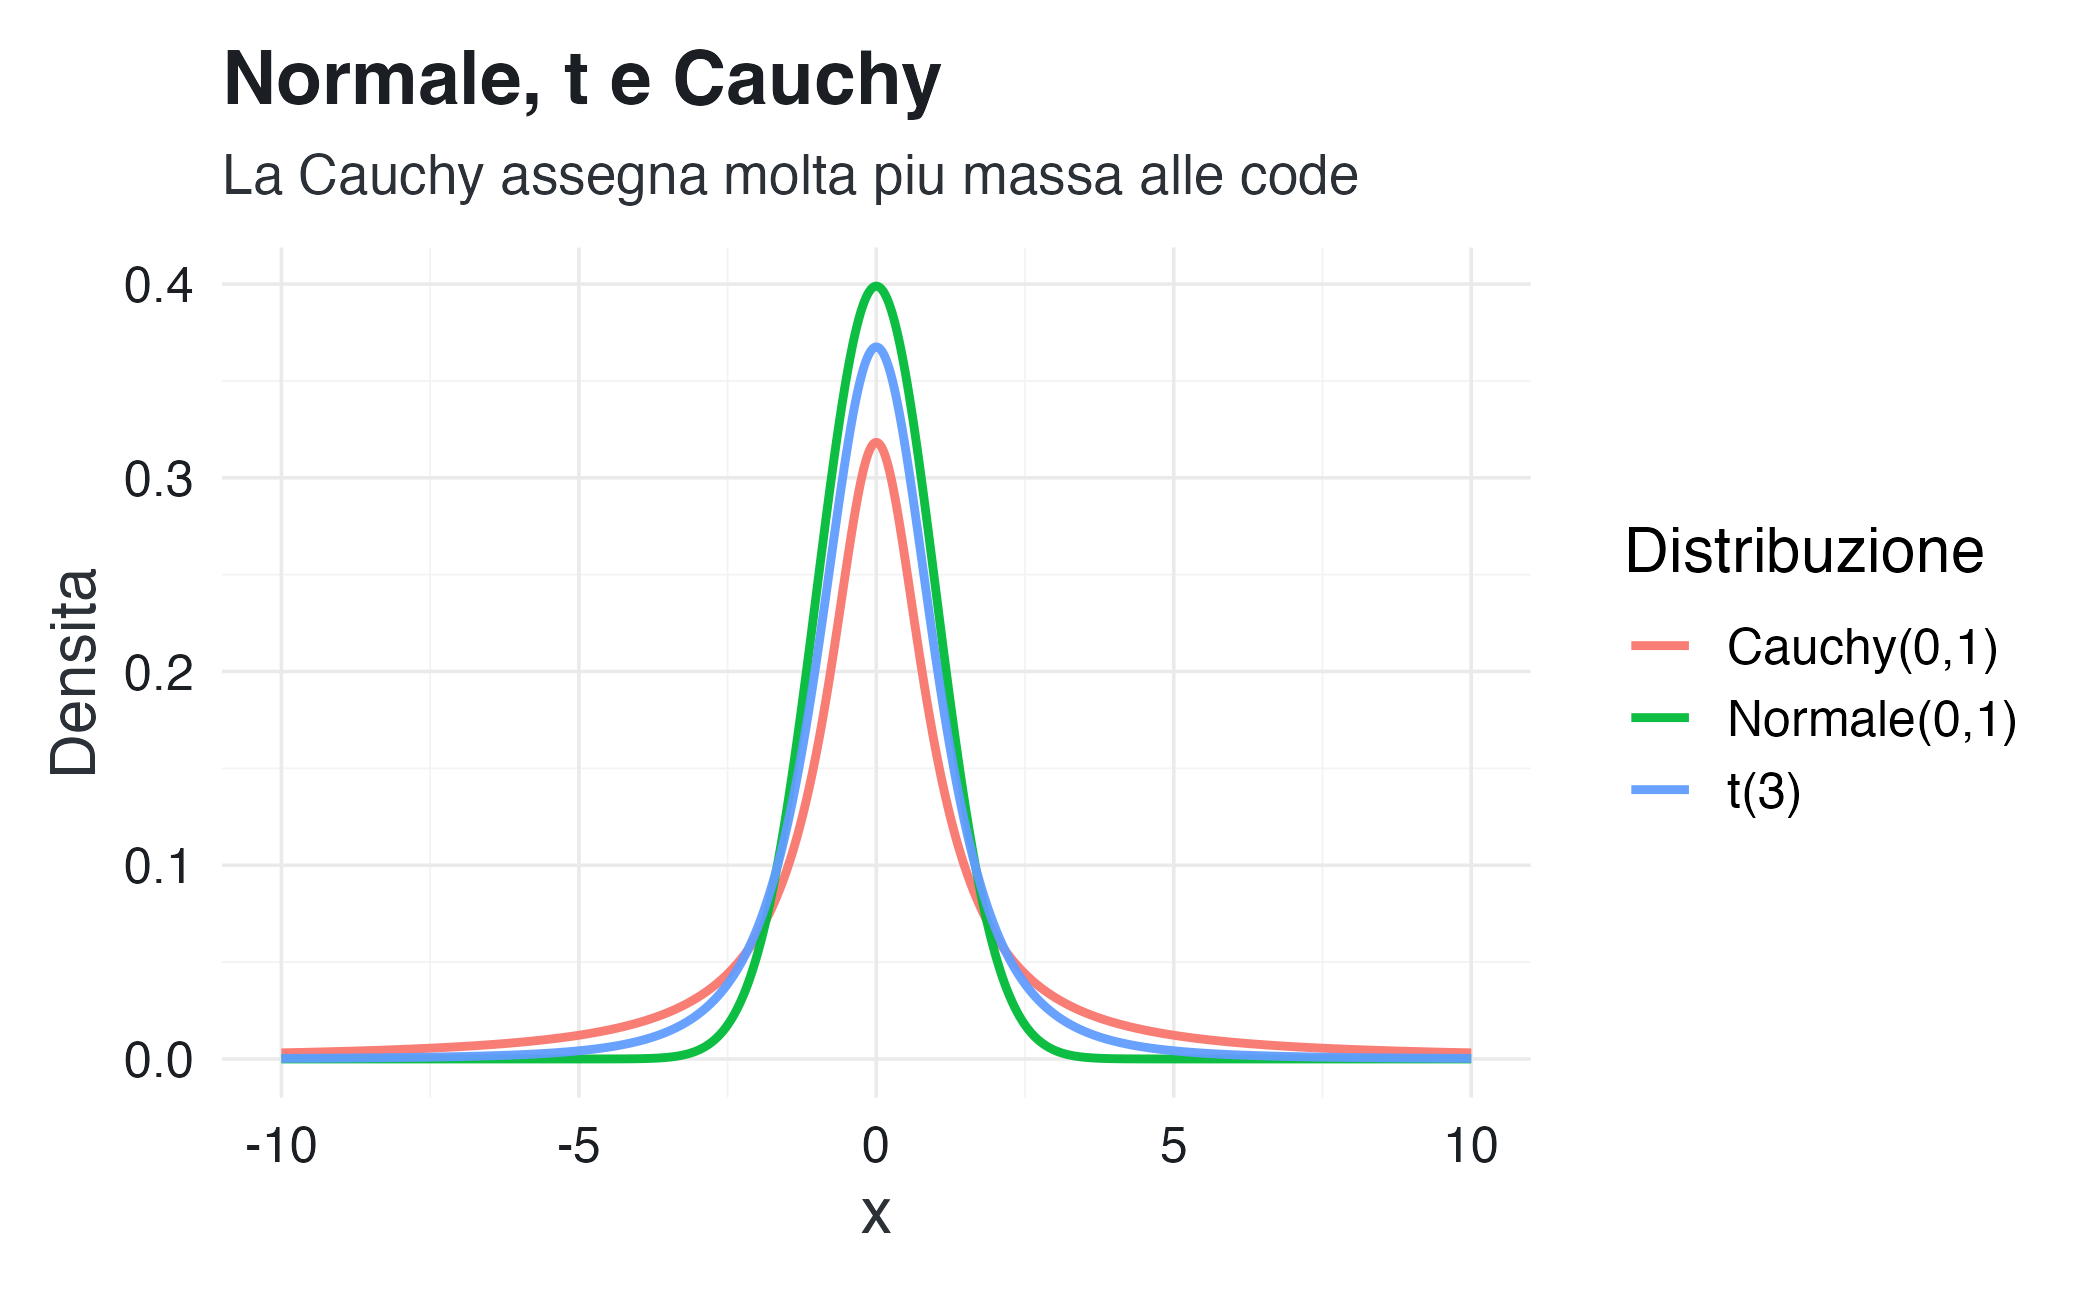
\includegraphics[width=0.85\linewidth,height=\textheight,keepaspectratio]{chapters/probability/12_cont_rv_distr_files/figure-pdf/unnamed-chunk-12-1.png}
\end{center}

\section{Come scegliere una distribuzione
continua?}\label{sec-cont-distribution-choice}

La scelta di una distribuzione non dovrebbe basarsi sulla convenienza
matematica, ma sulla struttura del problema. Tre domande aiutano a
orientarsi:

\subsection{1. Qual è il supporto?}\label{qual-uxe8-il-supporto}

\begin{itemize}
\tightlist
\item
  Se la quantità può assumere qualsiasi valore reale, le candidate sono
  la normale, la \(t\) o la Cauchy.
\item
  Se è positiva, si considerano l'esponenziale, la gamma o la
  log-normale.
\item
  Se è vincolata tra 0 e 1, la beta è spesso la scelta naturale.
\item
  Se invece è un conteggio, non siamo nel caso continuo: si torna alla
  Poisson, alla binomiale o ad altre distribuzioni discrete.
\end{itemize}

\subsection{2. Che forma ci aspettiamo?}\label{che-forma-ci-aspettiamo}

\begin{itemize}
\tightlist
\item
  Simmetria attorno a un centro: normale o \(t\).
\item
  Asimmetria positiva: gamma o log-normale.
\item
  Probabilità/proporzioni vincolate: beta.
\item
  Code molto pesanti: \(t\) con pochi gradi di libertà.
\end{itemize}

\subsection{3. Che ruolo ha la
distribuzione?}\label{che-ruolo-ha-la-distribuzione}

La stessa famiglia può avere ruoli diversi, ad esempio:

\begin{itemize}
\tightlist
\item
  la normale può essere un modello per dati continui o una prior per un
  effetto;
\item
  la beta è spesso una prior per una probabilità, ma può anche modellare
  dati continui proporzionali;
\item
  la gamma può modellare tempi positivi oppure essere una prior per un
  tasso;
\item
  la \(t\) può essere un modello robusto per dati o una prior robusta
  per parametri.
\end{itemize}

\begin{tcolorbox}[enhanced jigsaw, arc=.35mm, bottomrule=.15mm, bottomtitle=1mm, breakable, colback=white, colbacktitle=quarto-callout-important-color!10!white, colframe=quarto-callout-important-color-frame, coltitle=black, left=2mm, leftrule=.75mm, opacityback=0, opacitybacktitle=0.6, rightrule=.15mm, title=\textcolor{quarto-callout-important-color}{\faExclamation}\hspace{0.5em}{Modello generativo prima dell'inferenza}, titlerule=0mm, toprule=.15mm, toptitle=1mm]

Prima di chiedersi come aggiornare una credenza, occorre chiarire quale
modello collega il parametro ai dati osservabili. Questo capitolo
fornisce il vocabolario delle distribuzioni continue; il
Capitolo~\ref{sec-prob-inference-uncertainty} mostrerà come un campione
generato da questi modelli risulti più o meno informativo.

\end{tcolorbox}

\section*{Riflessioni conclusive}\label{riflessioni-conclusive-11}

\markright{Riflessioni conclusive}

Le distribuzioni continue completano il vocabolario avviato con quelle
discrete, consentendo di descrivere dati e parametri che si collocano su
scale continue: punteggi, durate, tassi, probabilità, effetti e
grandezze positive.

La prospettiva bayesiana aiuta a mantenere distinti i ruoli:

\begin{itemize}
\tightlist
\item
  una distribuzione può descrivere \textbf{dati osservabili
  condizionatamente a un parametro};
\item
  una distribuzione può rappresentare \textbf{incertezza epistemica su
  un parametro};
\item
  una volta osservati i dati, lo stesso modello può diventare una
  \textbf{funzione di verosimiglianza}.
\end{itemize}

Questa distinzione previene una confusione comune: la beta, ad esempio,
non è di solito un modello per una sequenza di risposte corrette/errate,
bensì una distribuzione su una probabilità. La binomiale descrive i
conteggi osservati; la beta, l'incertezza sul parametro che li genera.

Nel prossimo capitolo useremo questo vocabolario per affrontare una
nuova domanda: \textbf{quanto è informativo un campione?} Vedremo che
media campionaria, errore standard, precisione, Legge dei Grandi Numeri
e Teorema del Limite Centrale spiegano perché i dati possono
stabilizzare o modificare le nostre credenze.

\section*{Punti chiave da ricordare}\label{punti-chiave-da-ricordare-11}
\addcontentsline{toc}{section}{Punti chiave da ricordare}

\markright{Punti chiave da ricordare}

\begin{tcolorbox}[enhanced jigsaw, arc=.35mm, bottomrule=.15mm, bottomtitle=1mm, breakable, colback=white, colbacktitle=quarto-callout-important-color!10!white, colframe=quarto-callout-important-color-frame, coltitle=black, left=2mm, leftrule=.75mm, opacityback=0, opacitybacktitle=0.6, rightrule=.15mm, title=\textcolor{quarto-callout-important-color}{\faExclamation}\hspace{0.5em}{Importante}, titlerule=0mm, toprule=.15mm, toptitle=1mm]

\begin{enumerate}
\def\labelenumi{\arabic{enumi}.}
\tightlist
\item
  \textbf{Nel caso continuo, le probabilita sono aree}

  \begin{itemize}
  \tightlist
  \item
    Per una variabile continua, in genere \(P(X=x)=0\).
  \item
    La densita \(f(x)\) non e una probabilita puntuale.
  \item
    \(P(a \leq X \leq b)=\int_a^b f(x)\,dx\).
  \end{itemize}
\item
  \textbf{Il supporto guida la scelta del modello}

  \begin{itemize}
  \tightlist
  \item
    \(\mathbb{R}\): normale, \(t\), Cauchy.
  \item
    \((0,\infty)\): esponenziale, gamma.
  \item
    \((0,1)\): beta.
  \end{itemize}
\item
  \textbf{La normale e centrale, ma non universale}

  \begin{itemize}
  \tightlist
  \item
    Utile per errori additivi, punteggi standardizzati, effetti
    continui.
  \item
    Non adatta automaticamente a tempi, conteggi, proporzioni o scale
    ordinali.
  \end{itemize}
\item
  \textbf{La gamma e utile per quantita positive}

  \begin{itemize}
  \tightlist
  \item
    Include l'esponenziale come caso particolare.
  \item
    E naturale per tassi, durate, precisioni e processi positivi.
  \end{itemize}
\item
  \textbf{La beta rappresenta incertezza su probabilita}

  \begin{itemize}
  \tightlist
  \item
    Supporto \((0,1)\).
  \item
    Coniugata con Bernoulli e binomiale.
  \item
    Essenziale per inferenza bayesiana su proporzioni.
  \end{itemize}
\item
  \textbf{Le distribuzioni a code pesanti aumentano la robustezza}

  \begin{itemize}
  \tightlist
  \item
    La \(t\) e piu robusta della normale.
  \item
    La Cauchy e ancora piu permissiva nelle code.
  \item
    Robustezza non significa assenza di assunzioni.
  \end{itemize}
\item
  \textbf{Le distribuzioni sono strumenti modellistici}

  \begin{itemize}
  \tightlist
  \item
    Non sono fotografie della realta.
  \item
    Sono modi espliciti per rappresentare assunzioni su dati, parametri
    e incertezza.
  \end{itemize}
\end{enumerate}

\textbf{Formule da ricordare}

Normale:

\[
X \sim \mathcal{N}(\mu,\sigma^2),
\qquad
\mathbb{E}(X)=\mu,
\qquad
\mathbb{V}(X)=\sigma^2.
\]

Gamma, parametrizzazione shape-rate:

\[
X \sim \mathrm{Gamma}(\alpha,\beta),
\qquad
\mathbb{E}(X)=\frac{\alpha}{\beta},
\qquad
\mathbb{V}(X)=\frac{\alpha}{\beta^2}.
\]

Beta:

\[
\theta \sim \mathrm{Beta}(\alpha,\beta),
\qquad
\mathbb{E}(\theta)=\frac{\alpha}{\alpha+\beta}.
\]

Esponenziale:

\[
T \sim \mathrm{Exp}(\lambda),
\qquad
\mathbb{E}(T)=\frac{1}{\lambda}.
\]

\textbf{Per il prossimo capitolo}

Nel Capitolo~\ref{sec-prob-inference-uncertainty} useremo le
distribuzioni appena studiate per capire come un campione produce
evidenza: perché le medie campionarie fluttuano, in che modo l'errore
standard misura la precisione e in che senso i campioni più grandi
rendono l'evidenza più stabile.

\end{tcolorbox}

\begin{tcolorbox}[enhanced jigsaw, arc=.35mm, bottomrule=.15mm, bottomtitle=1mm, breakable, colback=white, colbacktitle=quarto-callout-note-color!10!white, colframe=quarto-callout-note-color-frame, coltitle=black, left=2mm, leftrule=.75mm, opacityback=0, opacitybacktitle=0.6, rightrule=.15mm, title=\textcolor{quarto-callout-note-color}{\faInfo}\hspace{0.5em}{Informazioni sull'ambiente di sviluppo}, titlerule=0mm, toprule=.15mm, toptitle=1mm]

\begin{Shaded}
\begin{Highlighting}[]
\FunctionTok{sessionInfo}\NormalTok{()}
\CommentTok{\#\textgreater{} R version 4.6.1 (2026{-}06{-}24)}
\CommentTok{\#\textgreater{} Platform: aarch64{-}apple{-}darwin23}
\CommentTok{\#\textgreater{} Running under: macOS Tahoe 26.5.2}
\CommentTok{\#\textgreater{} }
\CommentTok{\#\textgreater{} Matrix products: default}
\CommentTok{\#\textgreater{} BLAS:   /Library/Frameworks/R.framework/Versions/4.6/Resources/lib/libRblas.0.dylib }
\CommentTok{\#\textgreater{} LAPACK: /Library/Frameworks/R.framework/Versions/4.6/Resources/lib/libRlapack.dylib;  LAPACK version 3.12.1}
\CommentTok{\#\textgreater{} }
\CommentTok{\#\textgreater{} locale:}
\CommentTok{\#\textgreater{} [1] C.UTF{-}8/UTF{-}8/C.UTF{-}8/C/C.UTF{-}8/C.UTF{-}8}
\CommentTok{\#\textgreater{} }
\CommentTok{\#\textgreater{} time zone: Europe/Rome}
\CommentTok{\#\textgreater{} tzcode source: internal}
\CommentTok{\#\textgreater{} }
\CommentTok{\#\textgreater{} attached base packages:}
\CommentTok{\#\textgreater{} [1] stats     graphics  grDevices utils     datasets  methods   base     }
\CommentTok{\#\textgreater{} }
\CommentTok{\#\textgreater{} other attached packages:}
\CommentTok{\#\textgreater{}  [1] ragg\_1.5.2            tinytable\_0.17.0      withr\_3.0.3          }
\CommentTok{\#\textgreater{}  [4] systemfonts\_1.3.2     patchwork\_1.3.2       ggdist\_3.3.3         }
\CommentTok{\#\textgreater{}  [7] tidybayes\_3.0.7       bayesplot\_1.15.0      ggplot2\_4.0.3        }
\CommentTok{\#\textgreater{} [10] reliabilitydiag\_0.2.1 priorsense\_1.2.0      posterior\_1.7.0      }
\CommentTok{\#\textgreater{} [13] loo\_2.10.0            rstan\_2.32.7          StanHeaders\_2.32.10  }
\CommentTok{\#\textgreater{} [16] brms\_2.23.0           Rcpp\_1.1.2            sessioninfo\_1.2.4    }
\CommentTok{\#\textgreater{} [19] conflicted\_1.2.0      janitor\_2.2.1         matrixStats\_1.5.0    }
\CommentTok{\#\textgreater{} [22] modelr\_0.1.11         tibble\_3.3.1          dplyr\_1.2.1          }
\CommentTok{\#\textgreater{} [25] tidyr\_1.3.2           rio\_1.3.0             here\_1.0.2           }
\CommentTok{\#\textgreater{} }
\CommentTok{\#\textgreater{} loaded via a namespace (and not attached):}
\CommentTok{\#\textgreater{}  [1] svUnit\_1.0.8          tidyselect\_1.2.1      farver\_2.1.2         }
\CommentTok{\#\textgreater{}  [4] S7\_0.2.2              fastmap\_1.2.0         tensorA\_0.36.2.1     }
\CommentTok{\#\textgreater{}  [7] digest\_0.6.39         timechange\_0.4.0      estimability\_2.0.0   }
\CommentTok{\#\textgreater{} [10] lifecycle\_1.0.5       magrittr\_2.0.5        compiler\_4.6.1       }
\CommentTok{\#\textgreater{} [13] rlang\_1.3.0           tools\_4.6.1           knitr\_1.51           }
\CommentTok{\#\textgreater{} [16] labeling\_0.4.3        bridgesampling\_1.2{-}1  pkgbuild\_1.4.8       }
\CommentTok{\#\textgreater{} [19] curl\_7.1.0            RColorBrewer\_1.1{-}3    abind\_1.4{-}8          }
\CommentTok{\#\textgreater{} [22] purrr\_1.2.2           grid\_4.6.1            stats4\_4.6.1         }
\CommentTok{\#\textgreater{} [25] xtable\_1.8{-}8          inline\_0.3.21         emmeans\_2.0.3        }
\CommentTok{\#\textgreater{} [28] scales\_1.4.0          cli\_3.6.6             mvtnorm\_1.4{-}1        }
\CommentTok{\#\textgreater{} [31] rmarkdown\_2.31        generics\_0.1.4        otel\_0.2.0           }
\CommentTok{\#\textgreater{} [34] RcppParallel\_5.1.11{-}2 cachem\_1.1.0          stringr\_1.6.0        }
\CommentTok{\#\textgreater{} [37] parallel\_4.6.1        vctrs\_0.7.3           V8\_8.2.0             }
\CommentTok{\#\textgreater{} [40] Matrix\_1.7{-}5          jsonlite\_2.0.0        arrayhelpers\_1.1{-}1   }
\CommentTok{\#\textgreater{} [43] glue\_1.8.1            codetools\_0.2{-}20      distributional\_0.8.1 }
\CommentTok{\#\textgreater{} [46] lubridate\_1.9.5       stringi\_1.8.7         gtable\_0.3.6         }
\CommentTok{\#\textgreater{} [49] QuickJSR\_1.10.0       pillar\_1.11.1         htmltools\_0.5.9      }
\CommentTok{\#\textgreater{} [52] Brobdingnag\_1.2{-}9     R6\_2.6.1              textshaping\_1.0.5    }
\CommentTok{\#\textgreater{} [55] rprojroot\_2.1.1       evaluate\_1.0.5        lattice\_0.22{-}9       }
\CommentTok{\#\textgreater{} [58] backports\_1.5.1       memoise\_2.0.1         broom\_1.0.13         }
\CommentTok{\#\textgreater{} [61] snakecase\_0.11.1      rstantools\_2.6.0      coda\_0.19{-}4.1        }
\CommentTok{\#\textgreater{} [64] gridExtra\_2.3.1       nlme\_3.1{-}169          checkmate\_2.3.4      }
\CommentTok{\#\textgreater{} [67] xfun\_0.60             pkgconfig\_2.0.3}
\end{Highlighting}
\end{Shaded}

\end{tcolorbox}

\section*{Bibliografia}\label{bibliografia-6}

\markright{Bibliografia}

\part{PARTE 4: Verso l'inferenza}

\chapter{Dal campione all'evidenza: informazione, precisione e
incertezza}\label{sec-prob-inference-uncertainty}

\section*{Introduzione}\label{introduzione-12}

\markright{Introduzione}

Uno psicologo clinico sta valutando se adottare un nuovo protocollo per
la depressione. In uno studio pilota, il 36\% dei pazienti trattati ha
raggiunto la remissione completa dei sintomi. Il numero è incoraggiante,
ma da solo non basta per decidere: quanto potrebbe cambiare se lo studio
fosse ripetuto? Quanto è compatibile con un'efficacia reale del 30\%,
del 40\% o del 50\%? E quali aspetti dell'incertezza dipendono dal
campione, e quali invece dal modo in cui lo studio è stato progettato?

Questo capitolo affronta il passaggio dai dati osservati all'evidenza
statistica. Non introdurremo ancora in modo formale la funzione di
verosimiglianza: questo sarà il compito del capitolo successivo. Qui
prepariamo il terreno. L'obiettivo è capire \textbf{quanto informativo
sia un campione} e perché, al crescere della quantità di dati, alcune
ipotesi diventino più plausibili di altre.

La prospettiva rimane bayesiana. Le quantità ignote, ovvero le
proporzioni, le medie, le varianze o gli effetti, vengono trattate come
oggetti sui quali abbiamo incertezza epistemica. I dati non ``parlano da
soli'': diventano informativi solo all'interno di un modello
probabilistico che collega ciò che osserviamo ai parametri che vogliamo
conoscere.

La domanda guida del capitolo è quindi:

\begin{quote}
Che cosa rende un campione più o meno informativo rispetto a un
parametro ignoto?
\end{quote}

In questo capitolo:

\begin{enumerate}
\def\labelenumi{\arabic{enumi}.}
\tightlist
\item
  \textbf{collegheremo} dati osservati, parametri ignoti e modello
  generativo;
\item
  \textbf{rileggeremo} media e proporzione campionaria come riassunti
  dell'evidenza;
\item
  \textbf{introdurremo} la distribuzione campionaria come descrizione
  delle fluttuazioni attese dei dati;
\item
  \textbf{interpreteremo} errore standard e precisione come misure di
  informatività;
\item
  \textbf{useremo} la Legge dei Grandi Numeri e il Teorema del Limite
  Centrale per capire perché l'evidenza si stabilizza;
\item
  \textbf{discuteremo} il ruolo delle credenze a priori, dell'analisi di
  sensibilità e dei bias sistematici;
\item
  \textbf{chiuderemo} mostrando perché il passo successivo naturale è la
  funzione di verosimiglianza.
\end{enumerate}

\begin{tcolorbox}[enhanced jigsaw, arc=.35mm, bottomrule=.15mm, bottomtitle=1mm, breakable, colback=white, colbacktitle=quarto-callout-tip-color!10!white, colframe=quarto-callout-tip-color-frame, coltitle=black, left=2mm, leftrule=.75mm, opacityback=0, opacitybacktitle=0.6, rightrule=.15mm, title=\textcolor{quarto-callout-tip-color}{\faLightbulb}\hspace{0.5em}{Prerequisiti}, titlerule=0mm, toprule=.15mm, toptitle=1mm]

Per seguire questo capitolo è utile aver letto:

\begin{itemize}
\tightlist
\item
  Capitolo~\ref{sec-prob-bayes-theorem} --- per il meccanismo generale
  dell'aggiornamento bayesiano;
\item
  Capitolo~\ref{sec-prob-random-var} --- per il concetto di variabile
  casuale;
\item
  Capitolo~\ref{sec-prob-random-var-properties} --- per valore atteso,
  varianza ed errore standard;
\item
  1, 2 e Capitolo~\ref{sec-prob-cont-distr} --- per le principali
  famiglie di distribuzioni.
\end{itemize}

Questo capitolo funge da \textbf{ponte} tra lo studio delle
distribuzioni di probabilità e l'introduzione della verosimiglianza.

\end{tcolorbox}

\begin{tcolorbox}[enhanced jigsaw, arc=.35mm, bottomrule=.15mm, bottomtitle=1mm, breakable, colback=white, colbacktitle=quarto-callout-caution-color!10!white, colframe=quarto-callout-caution-color-frame, coltitle=black, left=2mm, leftrule=.75mm, opacityback=0, opacitybacktitle=0.6, rightrule=.15mm, title=\textcolor{quarto-callout-caution-color}{\faFire}\hspace{0.5em}{Preparazione del Notebook}, titlerule=0mm, toprule=.15mm, toptitle=1mm]

\begin{Shaded}
\begin{Highlighting}[]
\NormalTok{here}\SpecialCharTok{::}\FunctionTok{here}\NormalTok{(}\StringTok{"code"}\NormalTok{, }\StringTok{"\_common.R"}\NormalTok{) }\SpecialCharTok{|\textgreater{}} 
  \FunctionTok{source}\NormalTok{()}

\CommentTok{\# Riapplica il tema per sicurezza}
\FunctionTok{apply\_visual\_theme}\NormalTok{()}
\end{Highlighting}
\end{Shaded}

\end{tcolorbox}

\section{Dati, parametri e modello
generativo}\label{sec-data-parameters-generative-model}

\subsection{Il problema inferenziale}\label{il-problema-inferenziale}

Supponiamo di voler stimare la prevalenza \(\theta\) di studenti
universitari con sintomi depressivi clinicamente rilevanti. Se
selezioniamo un campione di \(n\) studenti e registriamo per ciascuno la
presenza o assenza del sintomo, otteniamo osservazioni binarie:

\[
X_i =
\begin{cases}
1 & \text{se lo studente } i \text{ presenta sintomi clinicamente rilevanti}, \\
0 & \text{altrimenti}.
\end{cases}
\]

Il parametro \(\theta\) rappresenta la proporzione del fenomeno nella
popolazione di riferimento. Non lo osserviamo direttamente: possiamo
solo raccogliere dati che, sotto opportune assunzioni, sono informativi
su di esso.

\subsection{Il modello generativo}\label{il-modello-generativo}

Un modello probabilistico semplice assume che, dato \(\theta\), ogni
osservazione segua una distribuzione di Bernoulli:

\[
X_i \mid \theta \sim \text{Bernoulli}(\theta), \qquad i = 1, \dots, n.
\]

Questa notazione va letta nel modo seguente: \textbf{se} il valore di
\(\theta\) fosse noto, potremmo descrivere probabilisticamente i dati
che ci aspettiamo di osservare. Ad esempio, se \(\theta = 0.30\), ogni
studente avrebbe una probabilità dello 0.30 di presentare il sintomo.

Dal punto di vista bayesiano, prima di osservare il campione possiamo
rappresentare la nostra incertezza su \(\theta\) con una distribuzione a
priori:

\[
\theta \sim p(\theta).
\]

Il modello completo ha quindi due componenti:

\[
\theta \sim p(\theta), \qquad X_i \mid \theta \sim p(x_i \mid \theta).
\]

La prima rappresenta ciò che sappiamo o assumiamo prima dei dati; la
seconda rappresenta il meccanismo che genera le osservazioni,
condizionatamente al parametro.

\begin{tcolorbox}[enhanced jigsaw, arc=.35mm, bottomrule=.15mm, bottomtitle=1mm, breakable, colback=white, colbacktitle=quarto-callout-note-color!10!white, colframe=quarto-callout-note-color-frame, coltitle=black, left=2mm, leftrule=.75mm, opacityback=0, opacitybacktitle=0.6, rightrule=.15mm, title=\textcolor{quarto-callout-note-color}{\faInfo}\hspace{0.5em}{Idea chiave}, titlerule=0mm, toprule=.15mm, toptitle=1mm]

Nel ragionamento bayesiano, i dati aggiornano le credenze solo
attraverso un modello. Non basta osservare una proporzione campionaria:
dobbiamo specificare quale processo probabilistico rende quella
proporzione più o meno attesa per diversi valori del parametro.

\end{tcolorbox}

\subsection{Il riassunto campionario}\label{il-riassunto-campionario}

Nel caso Bernoulliano, un riassunto naturale dei dati è la proporzione
campionaria:

\[
\bar{X} = \frac{1}{n}\sum_{i=1}^{n} X_i.
\]

Se osserviamo \(72\) studenti con sintomi su \(200\), allora:

\[
\bar{X} = \frac{72}{200} = 0.36.
\]

La proporzione osservata è una descrizione compatta del campione, ma non
è ancora una conclusione inferenziale. Per trasformarla in evidenza
dobbiamo chiederci: \textbf{quanto avrebbe potuto variare da un campione
all'altro?}

\section{Che cosa varia da un campione
all'altro}\label{sec-what-varies-across-samples}

\subsection{Media campionaria e valore
atteso}\label{media-campionaria-e-valore-atteso}

Siano \(X_1, X_2, \ldots, X_n\) variabili casuali indipendenti e
identicamente distribuite, con valore atteso
\(\mathbb{E}(X_i \mid \theta) = \theta\). La media campionaria è:

\[
\bar{X} = \frac{1}{n}\sum_{i=1}^{n} X_i.
\]

Per la linearità del valore atteso:

\[
\mathbb{E}(\bar{X} \mid \theta) = \theta.
\]

\textbf{Interpretazione.} Se potessimo ripetere molte volte lo stesso
studio, sempre con campioni della stessa dimensione e provenienti dallo
stesso processo generativo, la media delle proporzioni osservate sarebbe
centrata su \(\theta\). In questo senso, la proporzione campionaria non
tende sistematicamente a sovrastimare o sottostimare il parametro, a
condizione che il modello sia corretto e che il campionamento non
introduca bias.

\begin{tcolorbox}[enhanced jigsaw, arc=.35mm, bottomrule=.15mm, bottomtitle=1mm, breakable, colback=white, colbacktitle=quarto-callout-note-color!10!white, colframe=quarto-callout-note-color-frame, coltitle=black, left=2mm, leftrule=.75mm, opacityback=0, opacitybacktitle=0.6, rightrule=.15mm, title=\textcolor{quarto-callout-note-color}{\faInfo}\hspace{0.5em}{Dimostrazione}, titlerule=0mm, toprule=.15mm, toptitle=1mm]

\[
\mathbb{E}(\bar{X} \mid \theta)
= \mathbb{E}\left(\frac{1}{n}\sum_{i=1}^{n}X_i \mid \theta\right)
= \frac{1}{n}\sum_{i=1}^{n}\mathbb{E}(X_i \mid \theta)
= \frac{1}{n}\sum_{i=1}^{n}\theta
= \theta.
\]

\end{tcolorbox}

\subsection{Variabilità della media
campionaria}\label{variabilituxe0-della-media-campionaria}

Se le osservazioni \(X_1, \dots, X_n\) sono indipendenti e provengono da
una popolazione con varianza \(\sigma^2\), allora la varianza della loro
media è:

\[
\text{Var}(\bar{X} \mid \theta) = \frac{\sigma^2}{n}.
\]

Questa relazione ha una conseguenza pratica fondamentale: la precisione
della stima cresce con la \textbf{radice quadrata} della dimensione
campionaria. Per quantificare questa incertezza nella scala originale
dei dati, si utilizza l'\textbf{errore standard} (SE):

\[
\text{SE}(\bar{X}) = \sqrt{\text{Var}(\bar{X})} = \frac{\sigma}{\sqrt{n}}.
\]

L'errore standard misura quanto ci si può attendere che la media
campionaria oscilli da un campione all'altro. La sua espressione
\(\sigma/\sqrt{n}\) evidenzia una proprietà controintuitiva ma cruciale:
\textbf{l'incertezza non si riduce in proporzione diretta al numero di
osservazioni}. Per dimezzare l'errore standard non è sufficiente
raddoppiare il campione: occorre \textbf{quadruplicarlo}.

\begin{tcolorbox}[enhanced jigsaw, arc=.35mm, bottomrule=.15mm, bottomtitle=1mm, breakable, colback=white, colbacktitle=quarto-callout-note-color!10!white, colframe=quarto-callout-note-color-frame, coltitle=black, left=2mm, leftrule=.75mm, opacityback=0, opacitybacktitle=0.6, rightrule=.15mm, title=\textcolor{quarto-callout-note-color}{\faInfo}\hspace{0.5em}{Dimostrazione}, titlerule=0mm, toprule=.15mm, toptitle=1mm]

Per la proprietà di indipendenza delle osservazioni e la linearità della
varianza rispetto a costanti moltiplicative:

\[
\begin{aligned}
\text{Var}(\bar{X} \mid \theta)
&= \text{Var}\left(\frac{1}{n}\sum_{i=1}^{n}X_i \,\middle|\, \theta\right) \\
&= \frac{1}{n^2}\sum_{i=1}^{n}\text{Var}(X_i \mid \theta) \\
&= \frac{1}{n^2} \cdot n\sigma^2 = \frac{\sigma^2}{n}.
\end{aligned}
\]

\end{tcolorbox}

\subsection{Il caso Bernoulliano}\label{il-caso-bernoulliano}

Per una variabile Bernoulliana:

\[
\text{Var}(X_i \mid \theta) = \theta(1-\theta).
\]

Quindi:

\[
\text{Var}(\bar{X} \mid \theta) = \frac{\theta(1-\theta)}{n},
\qquad
\text{SE}(\bar{X}) = \sqrt{\frac{\theta(1-\theta)}{n}}.
\]

Poiché \(\theta\) è ignoto, nella pratica si usa spesso una stima
sostitutiva, per esempio \(\bar{X}\):

\[
\widehat{\text{SE}}(\bar{X}) = \sqrt{\frac{\bar{X}(1-\bar{X})}{n}}.
\]

Nel caso \(\bar{X}=0.36\) e \(n=200\):

\begin{Shaded}
\begin{Highlighting}[]
\NormalTok{p\_hat }\OtherTok{\textless{}{-}} \FloatTok{0.36}
\NormalTok{n }\OtherTok{\textless{}{-}} \DecValTok{200}
\NormalTok{se\_hat }\OtherTok{\textless{}{-}} \FunctionTok{sqrt}\NormalTok{(p\_hat }\SpecialCharTok{*}\NormalTok{ (}\DecValTok{1} \SpecialCharTok{{-}}\NormalTok{ p\_hat) }\SpecialCharTok{/}\NormalTok{ n)}
\NormalTok{se\_hat}
\CommentTok{\#\textgreater{} [1] 0.0339}
\end{Highlighting}
\end{Shaded}

L'ordine di grandezza dell'incertezza campionaria è quindi di circa
0.034. Questo non significa che l'efficacia reale sia certamente entro
\(0.36 \pm 0.034\), ma che campioni di quella dimensione producono
fluttuazioni tipiche di quell'ordine.

\section{La distribuzione
campionaria}\label{sec-sampling-distribution-evidence}

\subsection{Che cos'è una distribuzione
campionaria}\label{che-cosuxe8-una-distribuzione-campionaria}

Prima di raccogliere i dati, la media campionaria \(\bar{X}\) è una
variabile casuale: il suo valore è incerto e dipende da quale campione,
tra quelli possibili, verrà effettivamente osservato. Se fosse possibile
ripetere lo stesso studio un numero molto elevato di volte, otterremmo
una sequenza di valori \(\bar{X}_1, \bar{X}_2, \dots\), ciascuno
leggermente diverso dall'altro. La \textbf{distribuzione campionaria}
descrive esattamente questa variabilità: è la distribuzione di tutti i
possibili valori che \(\bar{X}\) potrebbe assumere in replicate ideali
del medesimo disegno di ricerca.

Questa idea è cruciale per l'inferenza statistica: \textbf{un dato
osservato è tanto più informativo quanto minore è la variabilità che ci
si aspetterebbe in caso di replicazione}. Se, in studi ripetuti, la
media campionaria tende a fluttuare poco attorno al valore vero, allora
l'osservazione che abbiamo effettuato restringe drasticamente l'insieme
dei valori plausibili del parametro. Se invece la distribuzione
campionaria è ampia, lo stesso dato potrebbe essere compatibile con
molti valori diversi del parametro, e la nostra conclusione sarà
inevitabilmente più incerta.

In questo senso, la distribuzione campionaria è ciò che trasforma un
numero osservato, ovvero una proporzione, una differenza tra medie o un
coefficiente di regressione, in una \textbf{misura di evidenza}: ci dice
quanto quel numero, da solo, possa vincolare le nostre credenze sul
mondo.

\subsection{Un esempio finito: risposte a un item
Likert}\label{un-esempio-finito-risposte-a-un-item-likert}

Consideriamo una piccola popolazione di quattro partecipanti con
risposte a un item di soddisfazione di vita:

\begin{Shaded}
\begin{Highlighting}[]
\NormalTok{risposte }\OtherTok{\textless{}{-}} \FunctionTok{c}\NormalTok{(}\DecValTok{2}\NormalTok{, }\DecValTok{4}\NormalTok{, }\DecValTok{4}\NormalTok{, }\DecValTok{5}\NormalTok{)}
\NormalTok{media\_pop }\OtherTok{\textless{}{-}} \FunctionTok{mean}\NormalTok{(risposte)}
\NormalTok{var\_pop }\OtherTok{\textless{}{-}} \FunctionTok{var}\NormalTok{(risposte) }\SpecialCharTok{*}\NormalTok{ ((}\FunctionTok{length}\NormalTok{(risposte) }\SpecialCharTok{{-}} \DecValTok{1}\NormalTok{) }\SpecialCharTok{/} \FunctionTok{length}\NormalTok{(risposte))}

\FunctionTok{cat}\NormalTok{(}\StringTok{"Media della popolazione:"}\NormalTok{, media\_pop, }\StringTok{"}\SpecialCharTok{\textbackslash{}n}\StringTok{"}\NormalTok{)}
\CommentTok{\#\textgreater{} Media della popolazione: 3.75}
\FunctionTok{cat}\NormalTok{(}\StringTok{"Varianza della popolazione:"}\NormalTok{, }\FunctionTok{round}\NormalTok{(var\_pop, }\DecValTok{3}\NormalTok{), }\StringTok{"}\SpecialCharTok{\textbackslash{}n}\StringTok{"}\NormalTok{)}
\CommentTok{\#\textgreater{} Varianza della popolazione: 1.19}
\end{Highlighting}
\end{Shaded}

Per comprendere la distribuzione campionaria, estraiamo tutti i
possibili campioni di dimensione \(n = 2\) \textbf{con reinserimento}
(campionamento con rimessa), generando \(4^2 = 16\) coppie ordinate. Per
ciascuna di esse calcoliamo la media \(\bar{X}\). L'elenco esaustivo è
il seguente:

\begin{Shaded}
\begin{Highlighting}[]
\NormalTok{campioni }\OtherTok{\textless{}{-}} \FunctionTok{expand.grid}\NormalTok{(risposte, risposte)}
\FunctionTok{colnames}\NormalTok{(campioni) }\OtherTok{\textless{}{-}} \FunctionTok{c}\NormalTok{(}\StringTok{"Partecipante\_1"}\NormalTok{, }\StringTok{"Partecipante\_2"}\NormalTok{)}
\NormalTok{medie\_campionarie }\OtherTok{\textless{}{-}} \FunctionTok{rowMeans}\NormalTok{(campioni)}

\NormalTok{df\_campioni }\OtherTok{\textless{}{-}} \FunctionTok{data.frame}\NormalTok{(}
  \AttributeTok{Campione =} \FunctionTok{paste0}\NormalTok{(}\StringTok{"("}\NormalTok{, campioni[,}\DecValTok{1}\NormalTok{], }\StringTok{", "}\NormalTok{, campioni[,}\DecValTok{2}\NormalTok{], }\StringTok{")"}\NormalTok{),}
  \AttributeTok{Media =} \FunctionTok{round}\NormalTok{(medie\_campionarie, }\DecValTok{1}\NormalTok{)}
\NormalTok{)}

\NormalTok{knitr}\SpecialCharTok{::}\FunctionTok{kable}\NormalTok{(df\_campioni, }
             \AttributeTok{caption =} \StringTok{"Tutti i 16 campioni di dimensione 2 (con reinserimento) e le relative medie"}\NormalTok{,}
             \AttributeTok{align =} \FunctionTok{c}\NormalTok{(}\StringTok{"c"}\NormalTok{, }\StringTok{"c"}\NormalTok{))}
\end{Highlighting}
\end{Shaded}

\begin{longtable}[]{@{}cc@{}}
\caption{Tutti i 16 campioni di dimensione 2 (con reinserimento) e le
relative medie}\tabularnewline
\toprule\noalign{}
Campione & Media \\
\midrule\noalign{}
\endfirsthead
\toprule\noalign{}
Campione & Media \\
\midrule\noalign{}
\endhead
\bottomrule\noalign{}
\endlastfoot
(2, 2) & 2.0 \\
(4, 2) & 3.0 \\
(4, 2) & 3.0 \\
(5, 2) & 3.5 \\
(2, 4) & 3.0 \\
(4, 4) & 4.0 \\
(4, 4) & 4.0 \\
(5, 4) & 4.5 \\
(2, 4) & 3.0 \\
(4, 4) & 4.0 \\
(4, 4) & 4.0 \\
(5, 4) & 4.5 \\
(2, 5) & 3.5 \\
(4, 5) & 4.5 \\
(4, 5) & 4.5 \\
(5, 5) & 5.0 \\
\end{longtable}

Ora rappresentiamo graficamente la distribuzione di queste 16 medie:

\begin{Shaded}
\begin{Highlighting}[]
\FunctionTok{ggplot}\NormalTok{(}\FunctionTok{data.frame}\NormalTok{(}\AttributeTok{media =}\NormalTok{ medie\_campionarie), }\FunctionTok{aes}\NormalTok{(}\AttributeTok{x =}\NormalTok{ media)) }\SpecialCharTok{+}
  \FunctionTok{geom\_histogram}\NormalTok{(}\FunctionTok{aes}\NormalTok{(}\AttributeTok{y =} \FunctionTok{after\_stat}\NormalTok{(density)), }\AttributeTok{binwidth =} \FloatTok{0.5}\NormalTok{, }\AttributeTok{boundary =} \DecValTok{0}\NormalTok{) }\SpecialCharTok{+}
  \FunctionTok{geom\_vline}\NormalTok{(}\AttributeTok{xintercept =}\NormalTok{ media\_pop, }\AttributeTok{linetype =} \StringTok{"dashed"}\NormalTok{, }\AttributeTok{linewidth =} \FloatTok{1.2}\NormalTok{, }\AttributeTok{color =} \StringTok{"red"}\NormalTok{) }\SpecialCharTok{+}
  \FunctionTok{labs}\NormalTok{(}
    \AttributeTok{title =} \StringTok{"Distribuzione campionaria della media (n = 2)"}\NormalTok{,}
    \AttributeTok{subtitle =} \StringTok{"La linea rossa tratteggiata indica la media della popolazione"}\NormalTok{,}
    \AttributeTok{x =} \StringTok{"Media campionaria"}\NormalTok{,}
    \AttributeTok{y =} \StringTok{"Densità"}
\NormalTok{  )}
\end{Highlighting}
\end{Shaded}

\begin{figure}[H]

{\centering 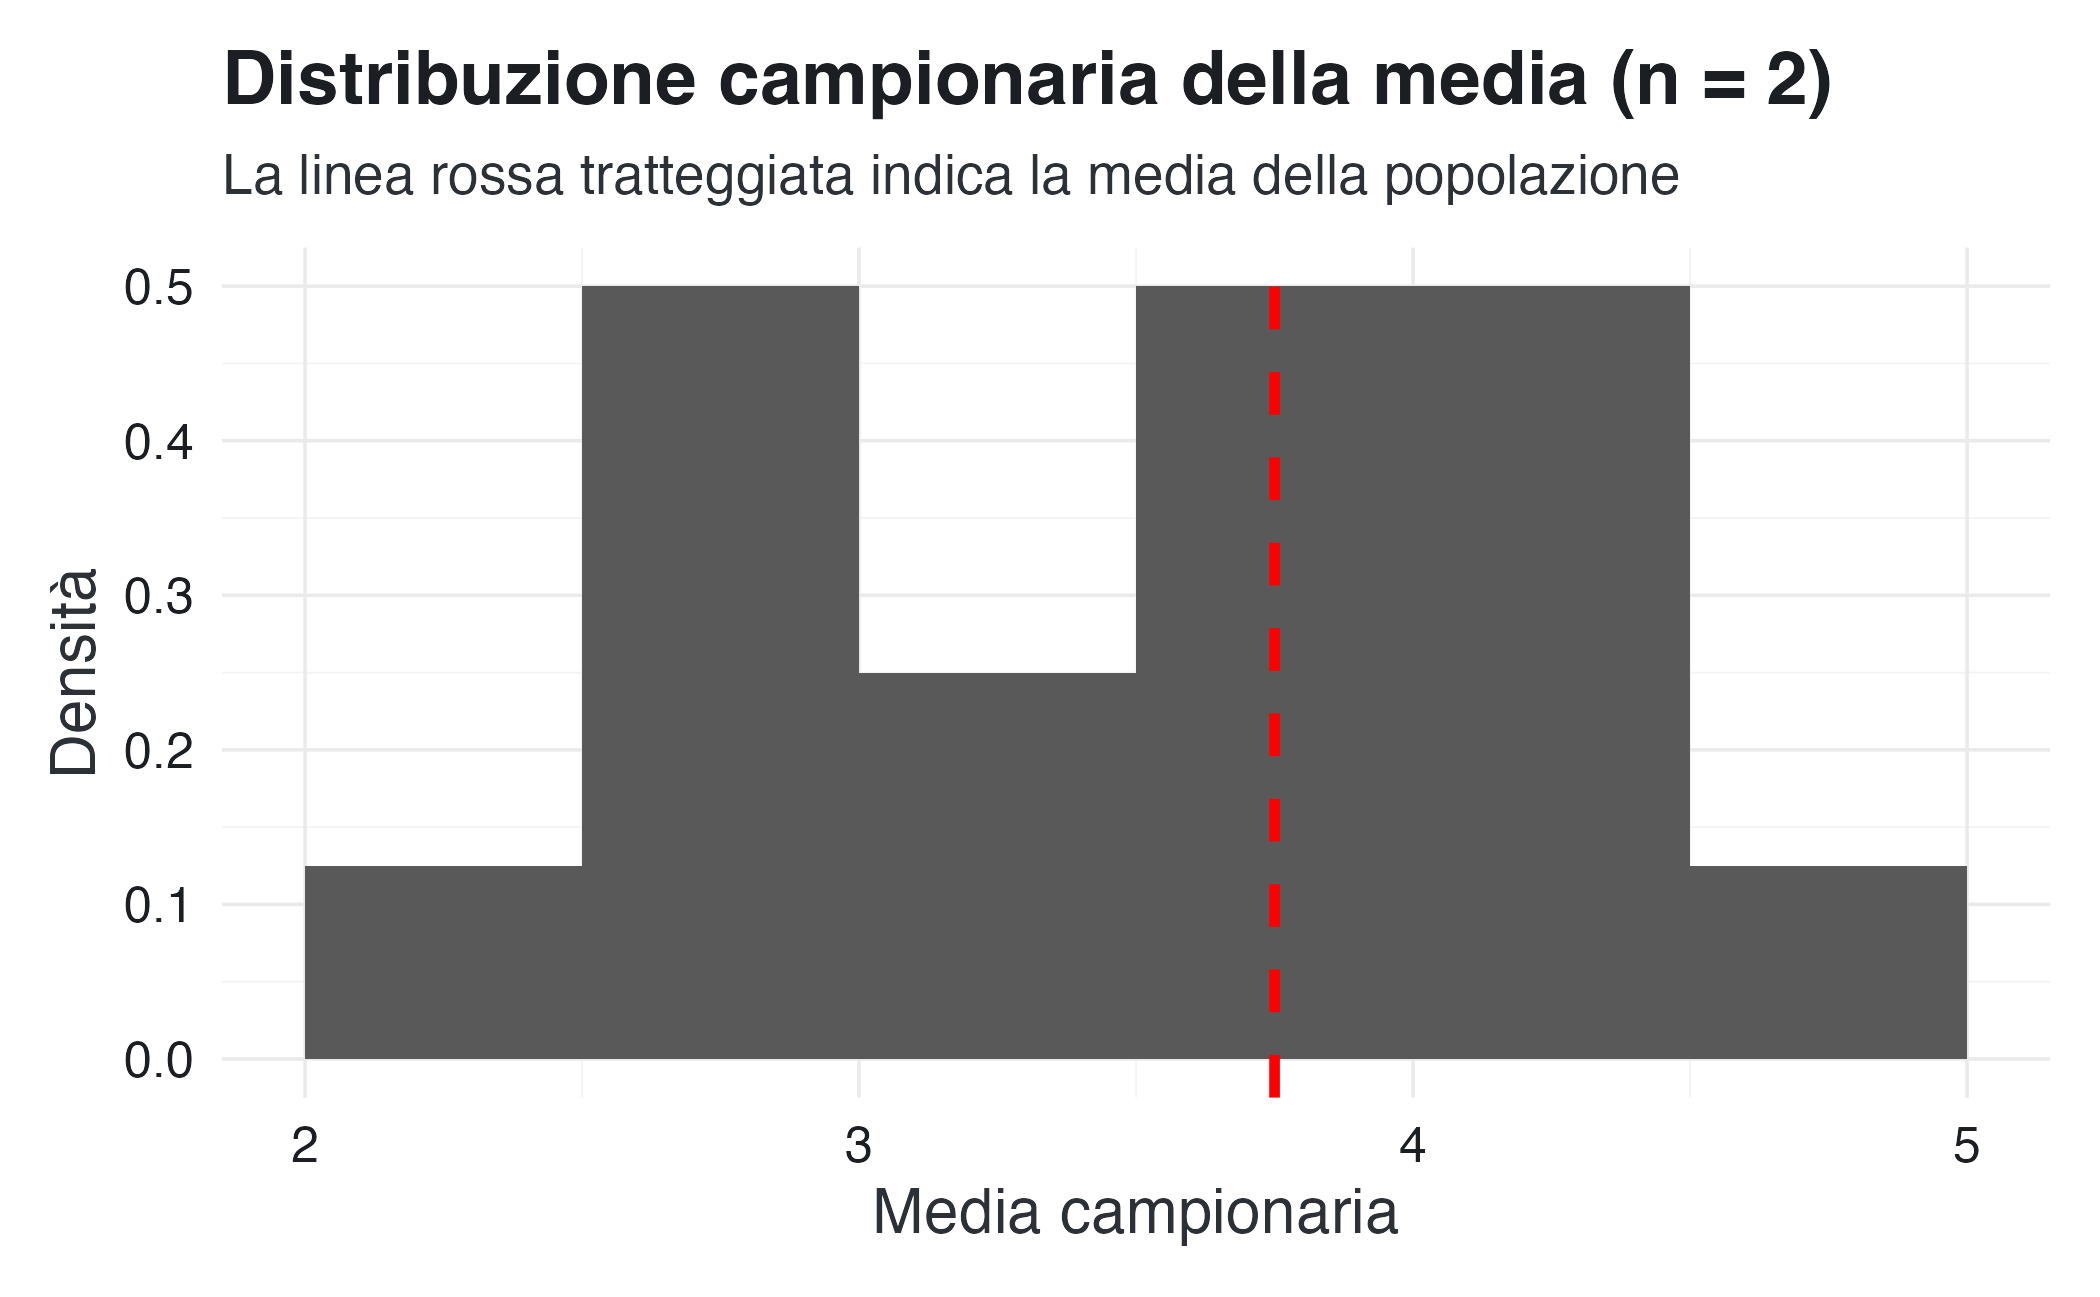
\includegraphics[width=0.85\linewidth,height=\textheight,keepaspectratio]{chapters/probability/13_from_sample_to_evidence_files/figure-pdf/sampling-distribution-likert-1.png}

}

\caption{Distribuzione campionaria della media per tutti i campioni di
dimensione 2 con reinserimento.}

\end{figure}%

Infine, verifichiamo numericamente le proprietà teoriche della
distribuzione campionaria:

\begin{Shaded}
\begin{Highlighting}[]
\FunctionTok{cat}\NormalTok{(}\StringTok{"Media delle medie campionarie:"}\NormalTok{, }\FunctionTok{mean}\NormalTok{(medie\_campionarie), }\StringTok{"}\SpecialCharTok{\textbackslash{}n}\StringTok{"}\NormalTok{)}
\CommentTok{\#\textgreater{} Media delle medie campionarie: 3.75}
\FunctionTok{cat}\NormalTok{(}\StringTok{"Media della popolazione:"}\NormalTok{, media\_pop, }\StringTok{"}\SpecialCharTok{\textbackslash{}n}\StringTok{"}\NormalTok{)}
\CommentTok{\#\textgreater{} Media della popolazione: 3.75}
\FunctionTok{cat}\NormalTok{(}\StringTok{"}\SpecialCharTok{\textbackslash{}n}\StringTok{"}\NormalTok{)}
\FunctionTok{cat}\NormalTok{(}\StringTok{"Varianza delle medie campionarie:"}\NormalTok{, }\FunctionTok{round}\NormalTok{(}\FunctionTok{var}\NormalTok{(medie\_campionarie) }\SpecialCharTok{*} \DecValTok{15} \SpecialCharTok{/} \DecValTok{16}\NormalTok{, }\DecValTok{3}\NormalTok{), }\StringTok{"}\SpecialCharTok{\textbackslash{}n}\StringTok{"}\NormalTok{)}
\CommentTok{\#\textgreater{} Varianza delle medie campionarie: 0.594}
\FunctionTok{cat}\NormalTok{(}\StringTok{"Varianza teorica (sigma\^{}2 / n):"}\NormalTok{, }\FunctionTok{round}\NormalTok{(var\_pop }\SpecialCharTok{/} \DecValTok{2}\NormalTok{, }\DecValTok{3}\NormalTok{), }\StringTok{"}\SpecialCharTok{\textbackslash{}n}\StringTok{"}\NormalTok{)}
\CommentTok{\#\textgreater{} Varianza teorica (sigma\^{}2 / n): 0.594}
\end{Highlighting}
\end{Shaded}

L'esempio mostra in modo concreto due fatti essenziali:

\begin{enumerate}
\def\labelenumi{\arabic{enumi}.}
\tightlist
\item
  \textbf{Le medie campionarie variano} da un campione all'altro,
  riflettendo l'incertezza intrinseca del campionamento.
\item
  \textbf{La distribuzione di queste medie è centrata sulla media della
  popolazione} e la sua variabilità è minore di quella delle singole
  osservazioni (la varianza delle medie è la metà della varianza della
  popolazione, poiché \(n = 2\)).
\end{enumerate}

\begin{tcolorbox}[enhanced jigsaw, arc=.35mm, bottomrule=.15mm, bottomtitle=1mm, breakable, colback=white, colbacktitle=quarto-callout-important-color!10!white, colframe=quarto-callout-important-color-frame, coltitle=black, left=2mm, leftrule=.75mm, opacityback=0, opacitybacktitle=0.6, rightrule=.15mm, title=\textcolor{quarto-callout-important-color}{\faExclamation}\hspace{0.5em}{Dal campione all'evidenza}, titlerule=0mm, toprule=.15mm, toptitle=1mm]

La distribuzione campionaria non è una parentesi frequentista estranea
alla prospettiva bayesiana. È il modo in cui il modello descrive quali
dati potremmo aspettarci prima di osservarli. Proprio questa descrizione
renderà possibile, nel capitolo successivo, valutare quali valori del
parametro rendono più plausibili i dati osservati.

\end{tcolorbox}

\section{Errore standard, precisione e
informazione}\label{sec-standard-error-precision-information}

\subsection{Errore standard come misura di incertezza
campionaria}\label{errore-standard-come-misura-di-incertezza-campionaria}

L'errore standard è la deviazione standard della distribuzione
campionaria di una statistica. Per la media:

\[
\text{SE}(\bar{X}) = \frac{\sigma}{\sqrt{n}}.
\]

Un errore standard piccolo indica che la media campionaria tende a
essere stabile da un campione all'altro. In termini inferenziali, il
dato è più informativo perché i valori lontani dal risultato osservato
diventano meno compatibili con il processo generativo.

Un errore standard grande indica invece che campioni diversi avrebbero
potuto produrre risultati molto diversi. In questo caso il dato
osservato è meno selettivo: molte ipotesi parametriche rimangono
compatibili con l'evidenza.

\subsection{Precisione come inverso della
varianza}\label{precisione-come-inverso-della-varianza}

Nell'inferenza bayesiana è spesso utile ragionare in termini di
\textbf{precisione}, definita come l'inverso della varianza:

\[
\tau = \frac{1}{\sigma^2}.
\]

Per la media campionaria:

\[
\text{Precisione}(\bar{X}) = \frac{1}{\text{Var}(\bar{X})} = \frac{n}{\sigma^2}.
\]

Quindi la precisione cresce linearmente con \(n\): ogni osservazione
aggiuntiva contribuisce informazione, anche se i guadagni in termini di
errore standard diventano progressivamente meno visibili.

\begin{tcolorbox}[enhanced jigsaw, arc=.35mm, bottomrule=.15mm, bottomtitle=1mm, breakable, colback=white, colbacktitle=quarto-callout-tip-color!10!white, colframe=quarto-callout-tip-color-frame, coltitle=black, left=2mm, leftrule=.75mm, opacityback=0, opacitybacktitle=0.6, rightrule=.15mm, title=\textcolor{quarto-callout-tip-color}{\faLightbulb}\hspace{0.5em}{Regola pratica}, titlerule=0mm, toprule=.15mm, toptitle=1mm]

Se l'errore standard è proporzionale a \(1/\sqrt{n}\), allora:

\begin{itemize}
\tightlist
\item
  per dimezzare l'errore standard occorre moltiplicare \(n\) per 4;
\item
  per ridurlo a un terzo occorre moltiplicare \(n\) per 9;
\item
  aumentare molto la precisione richiede spesso campioni molto più
  grandi di quanto l'intuizione suggerisca.
\end{itemize}

\end{tcolorbox}

\subsection{Combinare evidenze
indipendenti}\label{combinare-evidenze-indipendenti}

La precisione fornisce anche un'intuizione utile per la sintesi di più
studi. Supponiamo di avere due studi indipendenti sulla stessa quantità:

\begin{itemize}
\tightlist
\item
  Studio A: \(\hat{p}_A = 0.42\), \(\text{SE}_A = 0.07\);
\item
  Studio B: \(\hat{p}_B = 0.38\), \(\text{SE}_B = 0.035\).
\end{itemize}

Una combinazione approssimata, valida quando le stime sono trattabili
come gaussiane, pesa ciascuna stima in base alla sua precisione:

\[
\hat{p}_{\text{comb}} =
\frac{\tau_A \hat{p}_A + \tau_B \hat{p}_B}{\tau_A + \tau_B},
\qquad
\tau_j = \frac{1}{\text{SE}_j^2}.
\]

\begin{Shaded}
\begin{Highlighting}[]
\NormalTok{p\_hat\_A }\OtherTok{\textless{}{-}} \FloatTok{0.42}
\NormalTok{se\_A }\OtherTok{\textless{}{-}} \FloatTok{0.07}
\NormalTok{p\_hat\_B }\OtherTok{\textless{}{-}} \FloatTok{0.38}
\NormalTok{se\_B }\OtherTok{\textless{}{-}} \FloatTok{0.035}

\NormalTok{precisione\_A }\OtherTok{\textless{}{-}} \DecValTok{1} \SpecialCharTok{/}\NormalTok{ se\_A}\SpecialCharTok{\^{}}\DecValTok{2}
\NormalTok{precisione\_B }\OtherTok{\textless{}{-}} \DecValTok{1} \SpecialCharTok{/}\NormalTok{ se\_B}\SpecialCharTok{\^{}}\DecValTok{2}
\NormalTok{precisione\_combinata }\OtherTok{\textless{}{-}}\NormalTok{ precisione\_A }\SpecialCharTok{+}\NormalTok{ precisione\_B}
\NormalTok{p\_comb }\OtherTok{\textless{}{-}}\NormalTok{ (precisione\_A }\SpecialCharTok{*}\NormalTok{ p\_hat\_A }\SpecialCharTok{+}\NormalTok{ precisione\_B }\SpecialCharTok{*}\NormalTok{ p\_hat\_B) }\SpecialCharTok{/}\NormalTok{ precisione\_combinata}
\NormalTok{se\_comb }\OtherTok{\textless{}{-}} \FunctionTok{sqrt}\NormalTok{(}\DecValTok{1} \SpecialCharTok{/}\NormalTok{ precisione\_combinata)}

\FunctionTok{cat}\NormalTok{(}\StringTok{"Precisione A:"}\NormalTok{, }\FunctionTok{round}\NormalTok{(precisione\_A, }\DecValTok{1}\NormalTok{), }\StringTok{"}\SpecialCharTok{\textbackslash{}n}\StringTok{"}\NormalTok{)}
\CommentTok{\#\textgreater{} Precisione A: 204}
\FunctionTok{cat}\NormalTok{(}\StringTok{"Precisione B:"}\NormalTok{, }\FunctionTok{round}\NormalTok{(precisione\_B, }\DecValTok{1}\NormalTok{), }\StringTok{"}\SpecialCharTok{\textbackslash{}n}\StringTok{"}\NormalTok{)}
\CommentTok{\#\textgreater{} Precisione B: 816}
\FunctionTok{cat}\NormalTok{(}\StringTok{"Stima combinata:"}\NormalTok{, }\FunctionTok{round}\NormalTok{(p\_comb, }\DecValTok{3}\NormalTok{), }\StringTok{"}\SpecialCharTok{\textbackslash{}n}\StringTok{"}\NormalTok{)}
\CommentTok{\#\textgreater{} Stima combinata: 0.388}
\FunctionTok{cat}\NormalTok{(}\StringTok{"Errore standard combinato:"}\NormalTok{, }\FunctionTok{round}\NormalTok{(se\_comb, }\DecValTok{4}\NormalTok{), }\StringTok{"}\SpecialCharTok{\textbackslash{}n}\StringTok{"}\NormalTok{)}
\CommentTok{\#\textgreater{} Errore standard combinato: 0.0313}
\end{Highlighting}
\end{Shaded}

Lo Studio B pesa di più perché è più preciso. Questa stessa intuizione
tornerà nell'aggiornamento bayesiano: quando prior e dati sono
rappresentabili come distribuzioni gaussiane, la media a posteriori è
una media ponderata dalle rispettive precisioni.

\section{La Legge dei Grandi Numeri}\label{sec-lln-evidence}

\subsection{Enunciato intuitivo}\label{enunciato-intuitivo}

La \textbf{Legge dei Grandi Numeri} afferma che, all'aumentare del
numero di osservazioni, la media campionaria tende ad avvicinarsi al
valore atteso della distribuzione generativa:

\[
\bar{X}_n \longrightarrow \mu.
\]

Nel caso Bernoulliano, \(\mu=\theta\), quindi:

\[
\bar{X}_n \longrightarrow \theta.
\]

Il punto non è che ogni campione grande produca esattamente il valore
vero, ma che deviazioni grandi diventano progressivamente meno
probabili.

\subsection{Simulazione della
convergenza}\label{simulazione-della-convergenza}

\begin{Shaded}
\begin{Highlighting}[]
\FunctionTok{set.seed}\NormalTok{(}\DecValTok{42}\NormalTok{)}
\NormalTok{theta\_true }\OtherTok{\textless{}{-}} \FloatTok{0.45}
\NormalTok{n\_max }\OtherTok{\textless{}{-}} \DecValTok{1000}

\NormalTok{osservazioni }\OtherTok{\textless{}{-}} \FunctionTok{rbinom}\NormalTok{(n\_max, }\AttributeTok{size =} \DecValTok{1}\NormalTok{, }\AttributeTok{prob =}\NormalTok{ theta\_true)}
\NormalTok{medie\_cumulative }\OtherTok{\textless{}{-}} \FunctionTok{cumsum}\NormalTok{(osservazioni) }\SpecialCharTok{/} \FunctionTok{seq\_along}\NormalTok{(osservazioni)}

\NormalTok{data\_plot }\OtherTok{\textless{}{-}} \FunctionTok{data.frame}\NormalTok{(}
  \AttributeTok{n =} \DecValTok{1}\SpecialCharTok{:}\NormalTok{n\_max,}
  \AttributeTok{media =}\NormalTok{ medie\_cumulative}
\NormalTok{)}

\FunctionTok{ggplot}\NormalTok{(data\_plot, }\FunctionTok{aes}\NormalTok{(}\AttributeTok{x =}\NormalTok{ n, }\AttributeTok{y =}\NormalTok{ media)) }\SpecialCharTok{+}
  \FunctionTok{geom\_line}\NormalTok{(}\AttributeTok{linewidth =} \FloatTok{0.8}\NormalTok{, }\AttributeTok{alpha =} \FloatTok{0.8}\NormalTok{) }\SpecialCharTok{+}
  \FunctionTok{geom\_hline}\NormalTok{(}\AttributeTok{yintercept =}\NormalTok{ theta\_true, }\AttributeTok{linetype =} \StringTok{"dashed"}\NormalTok{, }\AttributeTok{linewidth =} \FloatTok{1.2}\NormalTok{) }\SpecialCharTok{+}
  \FunctionTok{labs}\NormalTok{(}
    \AttributeTok{title =} \StringTok{"Convergenza della proporzione campionaria"}\NormalTok{,}
    \AttributeTok{subtitle =} \StringTok{"La linea tratteggiata indica il valore generativo theta = 0.45"}\NormalTok{,}
    \AttributeTok{x =} \StringTok{"Numero di osservazioni"}\NormalTok{,}
    \AttributeTok{y =} \StringTok{"Proporzione cumulativa"}
\NormalTok{  )}
\end{Highlighting}
\end{Shaded}

\begin{figure}[H]

{\centering 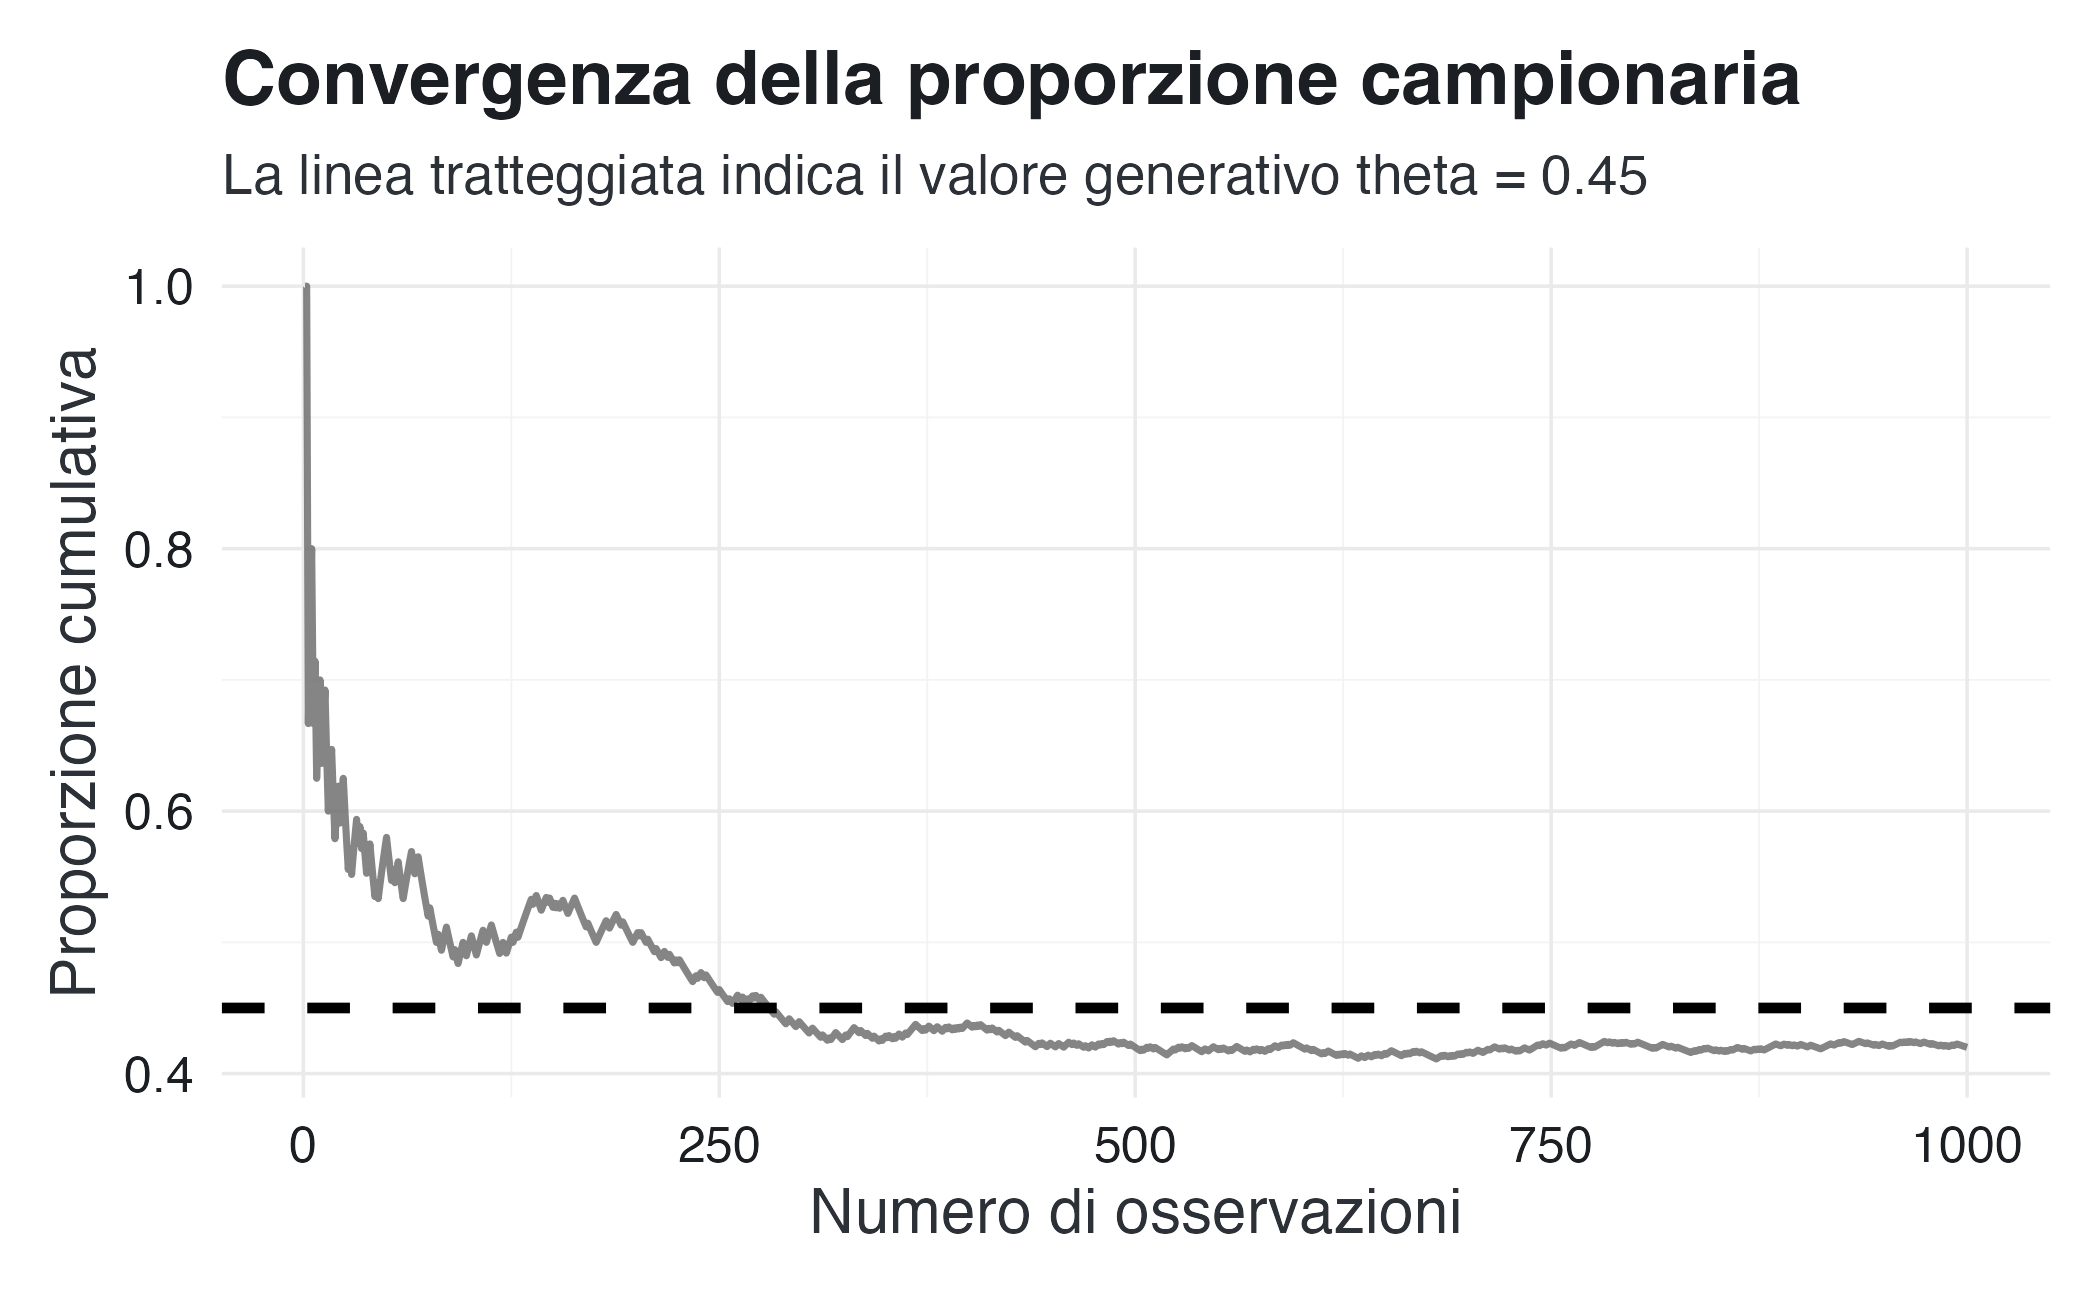
\includegraphics[width=0.85\linewidth,height=\textheight,keepaspectratio]{chapters/probability/13_from_sample_to_evidence_files/figure-pdf/lln-simulation-1.png}

}

\caption{Convergenza della proporzione campionaria al valore
generativo.}

\end{figure}%

Nelle prime osservazioni, la proporzione cumulativa oscilla molto. Con
l'aumentare di \(n\), le oscillazioni non scompaiono del tutto, ma
diventano più piccole rispetto alla scala complessiva del problema.

\subsection{Lettura bayesiana}\label{lettura-bayesiana}

Dal punto di vista bayesiano, la Legge dei Grandi Numeri spiega perché
l'evidenza empirica diventa progressivamente più vincolante. Se i dati
sono generati stabilmente da un modello con parametro \(\theta\),
campioni più grandi tenderanno a produrre riassunti campionari vicini a
quel valore. Di conseguenza, i valori parametrici incompatibili con quei
riassunti riceveranno sempre meno supporto dai dati.

Questa è l'intuizione alla base della \textbf{convergenza bayesiana}:
quando il modello è adeguato e la prior non esclude il valore vero,
l'accumularsi dei dati tende a far convergere osservatori con prior
diverse verso conclusioni simili.

\section{Il Teorema del Limite Centrale}\label{sec-clt-evidence}

\subsection{Enunciato intuitivo}\label{enunciato-intuitivo-1}

Il \textbf{Teorema del Limite Centrale} afferma che, per osservazioni
indipendenti e identicamente distribuite con valore atteso \(\mu\) e
varianza finita \(\sigma^2\), la distribuzione della media campionaria
diventa approssimativamente normale quando \(n\) è grande:

\[
\bar{X}_n \dot\sim \mathcal{N}\left(\mu, \frac{\sigma^2}{n}\right).
\]

Il risultato è sorprendente perché non richiede che la distribuzione
originaria sia normale. È la media campionaria a diventare
approssimativamente normale.

\subsection{Visualizzazione del
risultato}\label{visualizzazione-del-risultato}

\begin{Shaded}
\begin{Highlighting}[]
\FunctionTok{set.seed}\NormalTok{(}\DecValTok{42}\NormalTok{)}
\NormalTok{popolazione }\OtherTok{\textless{}{-}} \FunctionTok{runif}\NormalTok{(}\DecValTok{20000}\NormalTok{, }\AttributeTok{min =} \DecValTok{0}\NormalTok{, }\AttributeTok{max =} \DecValTok{1}\NormalTok{)}

\FunctionTok{ggplot}\NormalTok{(}\FunctionTok{data.frame}\NormalTok{(}\AttributeTok{x =}\NormalTok{ popolazione), }\FunctionTok{aes}\NormalTok{(}\AttributeTok{x =}\NormalTok{ x)) }\SpecialCharTok{+}
  \FunctionTok{geom\_histogram}\NormalTok{(}\FunctionTok{aes}\NormalTok{(}\AttributeTok{y =} \FunctionTok{after\_stat}\NormalTok{(density)), }\AttributeTok{bins =} \DecValTok{30}\NormalTok{) }\SpecialCharTok{+}
  \FunctionTok{labs}\NormalTok{(}
    \AttributeTok{title =} \StringTok{"Distribuzione della popolazione"}\NormalTok{,}
    \AttributeTok{subtitle =} \StringTok{"Popolazione uniforme: non normale"}\NormalTok{,}
    \AttributeTok{x =} \StringTok{"Valore"}\NormalTok{,}
    \AttributeTok{y =} \StringTok{"Densità"}
\NormalTok{  )}
\end{Highlighting}
\end{Shaded}

\begin{figure}[H]

{\centering 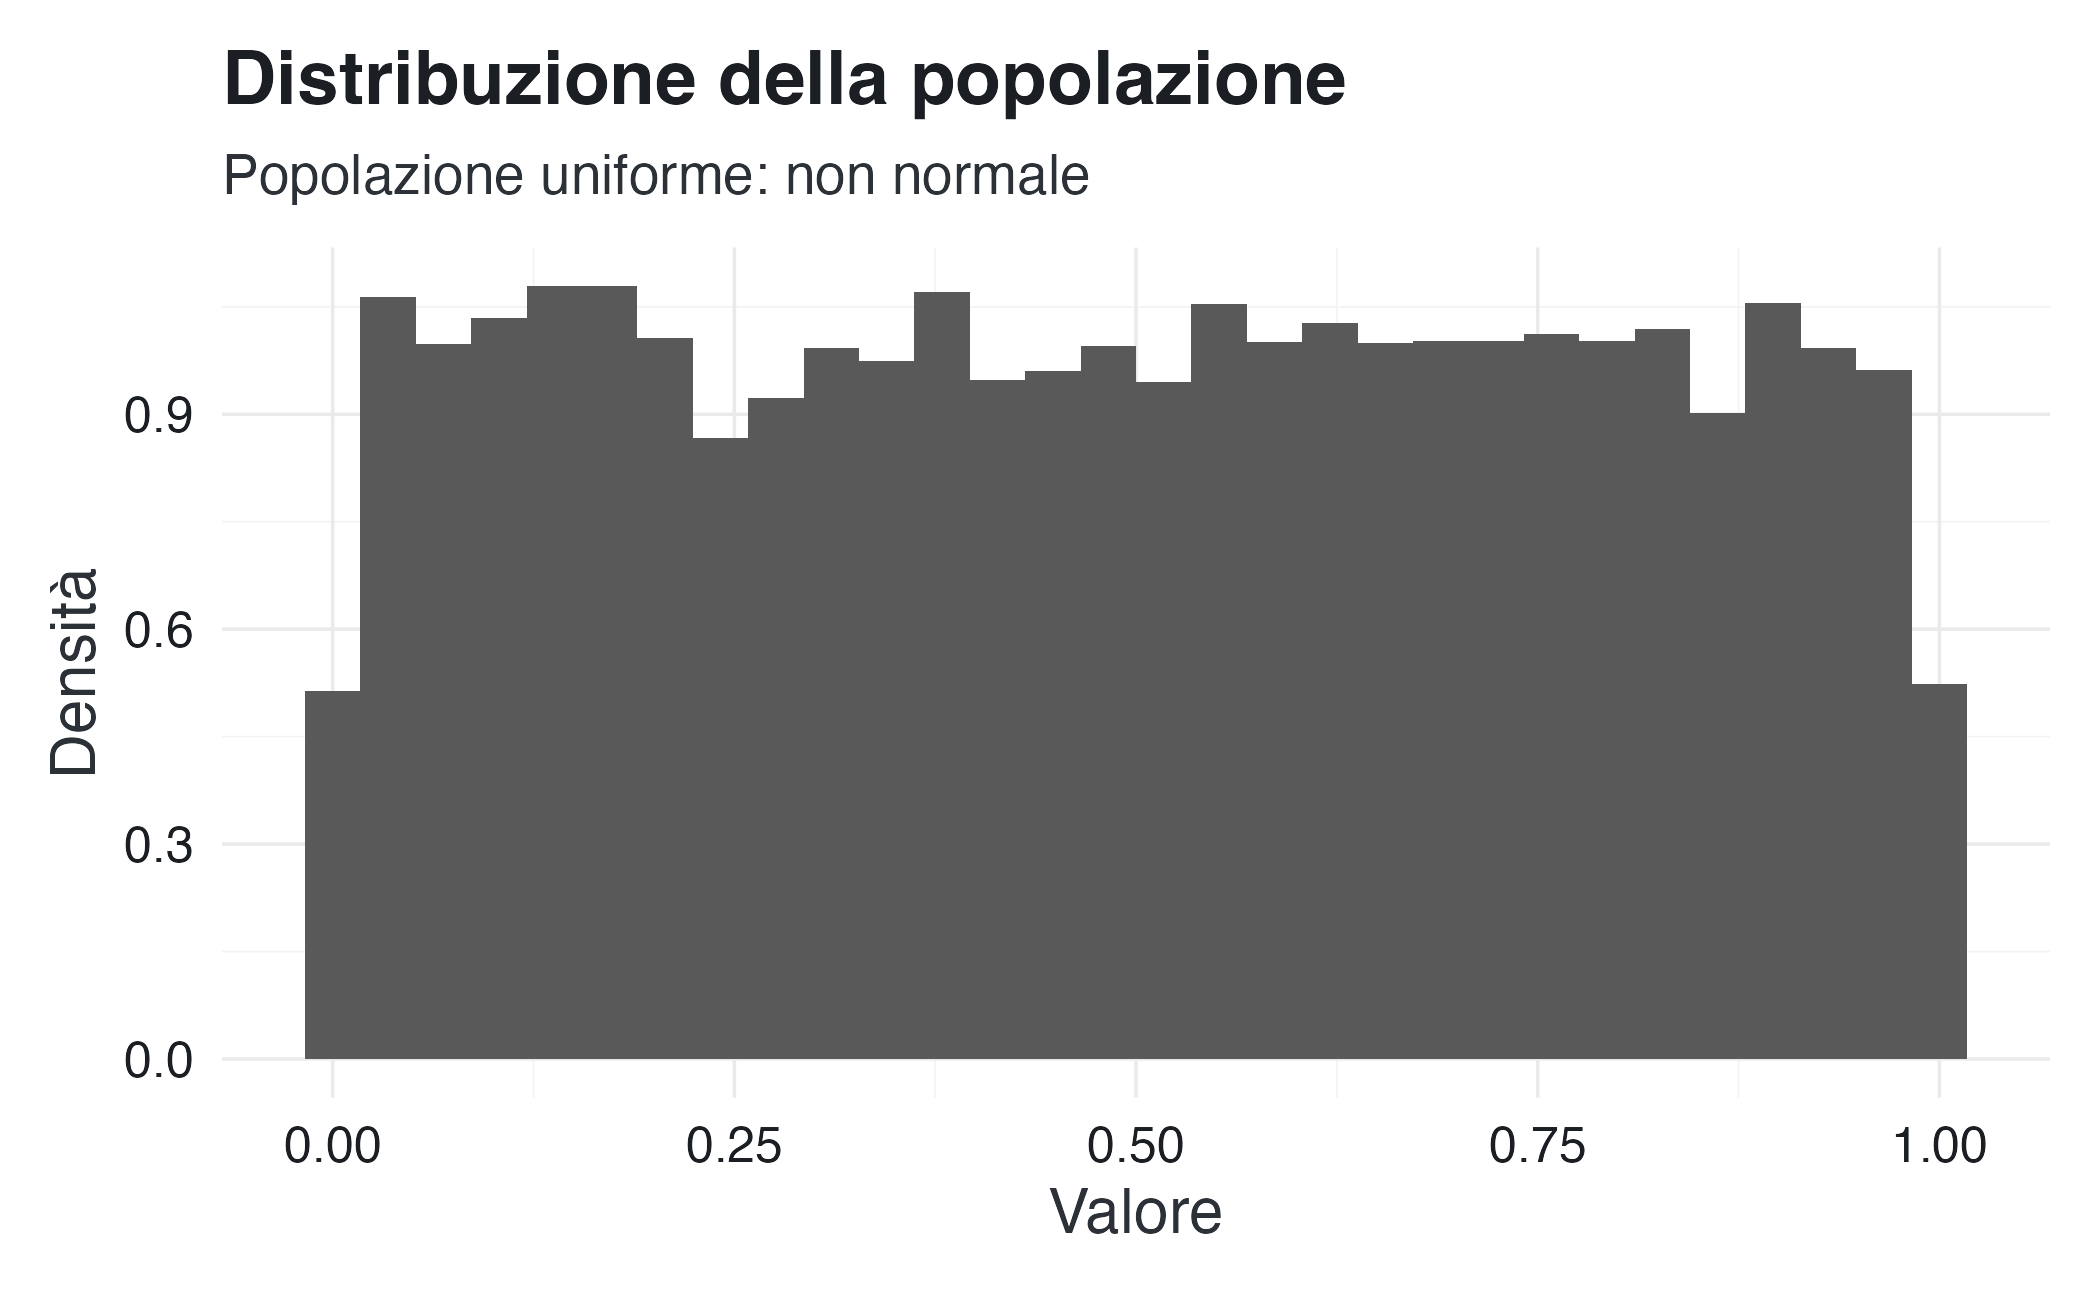
\includegraphics[width=0.85\linewidth,height=\textheight,keepaspectratio]{chapters/probability/13_from_sample_to_evidence_files/figure-pdf/clt-population-1.png}

}

\caption{Distribuzione originaria uniforme da cui vengono estratti i
campioni.}

\end{figure}%

\begin{Shaded}
\begin{Highlighting}[]
\NormalTok{n\_campione }\OtherTok{\textless{}{-}} \DecValTok{30}
\NormalTok{n\_ripetizioni }\OtherTok{\textless{}{-}} \DecValTok{1000}

\NormalTok{medie }\OtherTok{\textless{}{-}} \FunctionTok{replicate}\NormalTok{(n\_ripetizioni, \{}
\NormalTok{  campione }\OtherTok{\textless{}{-}} \FunctionTok{sample}\NormalTok{(popolazione, }\AttributeTok{size =}\NormalTok{ n\_campione, }\AttributeTok{replace =} \ConstantTok{TRUE}\NormalTok{)}
  \FunctionTok{mean}\NormalTok{(campione)}
\NormalTok{\})}

\NormalTok{x\_bar }\OtherTok{\textless{}{-}} \FunctionTok{mean}\NormalTok{(medie)}
\NormalTok{std }\OtherTok{\textless{}{-}} \FunctionTok{sd}\NormalTok{(medie)}

\FunctionTok{ggplot}\NormalTok{(}\FunctionTok{data.frame}\NormalTok{(}\AttributeTok{media =}\NormalTok{ medie), }\FunctionTok{aes}\NormalTok{(}\AttributeTok{x =}\NormalTok{ media)) }\SpecialCharTok{+}
  \FunctionTok{geom\_histogram}\NormalTok{(}\FunctionTok{aes}\NormalTok{(}\AttributeTok{y =} \FunctionTok{after\_stat}\NormalTok{(density)), }\AttributeTok{bins =} \DecValTok{30}\NormalTok{) }\SpecialCharTok{+}
  \FunctionTok{stat\_function}\NormalTok{(}\AttributeTok{fun =}\NormalTok{ dnorm, }\AttributeTok{args =} \FunctionTok{list}\NormalTok{(}\AttributeTok{mean =}\NormalTok{ x\_bar, }\AttributeTok{sd =}\NormalTok{ std), }\AttributeTok{linewidth =} \FloatTok{1.2}\NormalTok{) }\SpecialCharTok{+}
  \FunctionTok{labs}\NormalTok{(}
    \AttributeTok{title =} \StringTok{"Distribuzione delle medie campionarie"}\NormalTok{,}
    \AttributeTok{subtitle =} \StringTok{"La curva sovrapposta è una normale con media e deviazione standard empiriche"}\NormalTok{,}
    \AttributeTok{x =} \StringTok{"Media campionaria"}\NormalTok{,}
    \AttributeTok{y =} \StringTok{"Densità"}
\NormalTok{  )}
\end{Highlighting}
\end{Shaded}

\begin{figure}[H]

{\centering 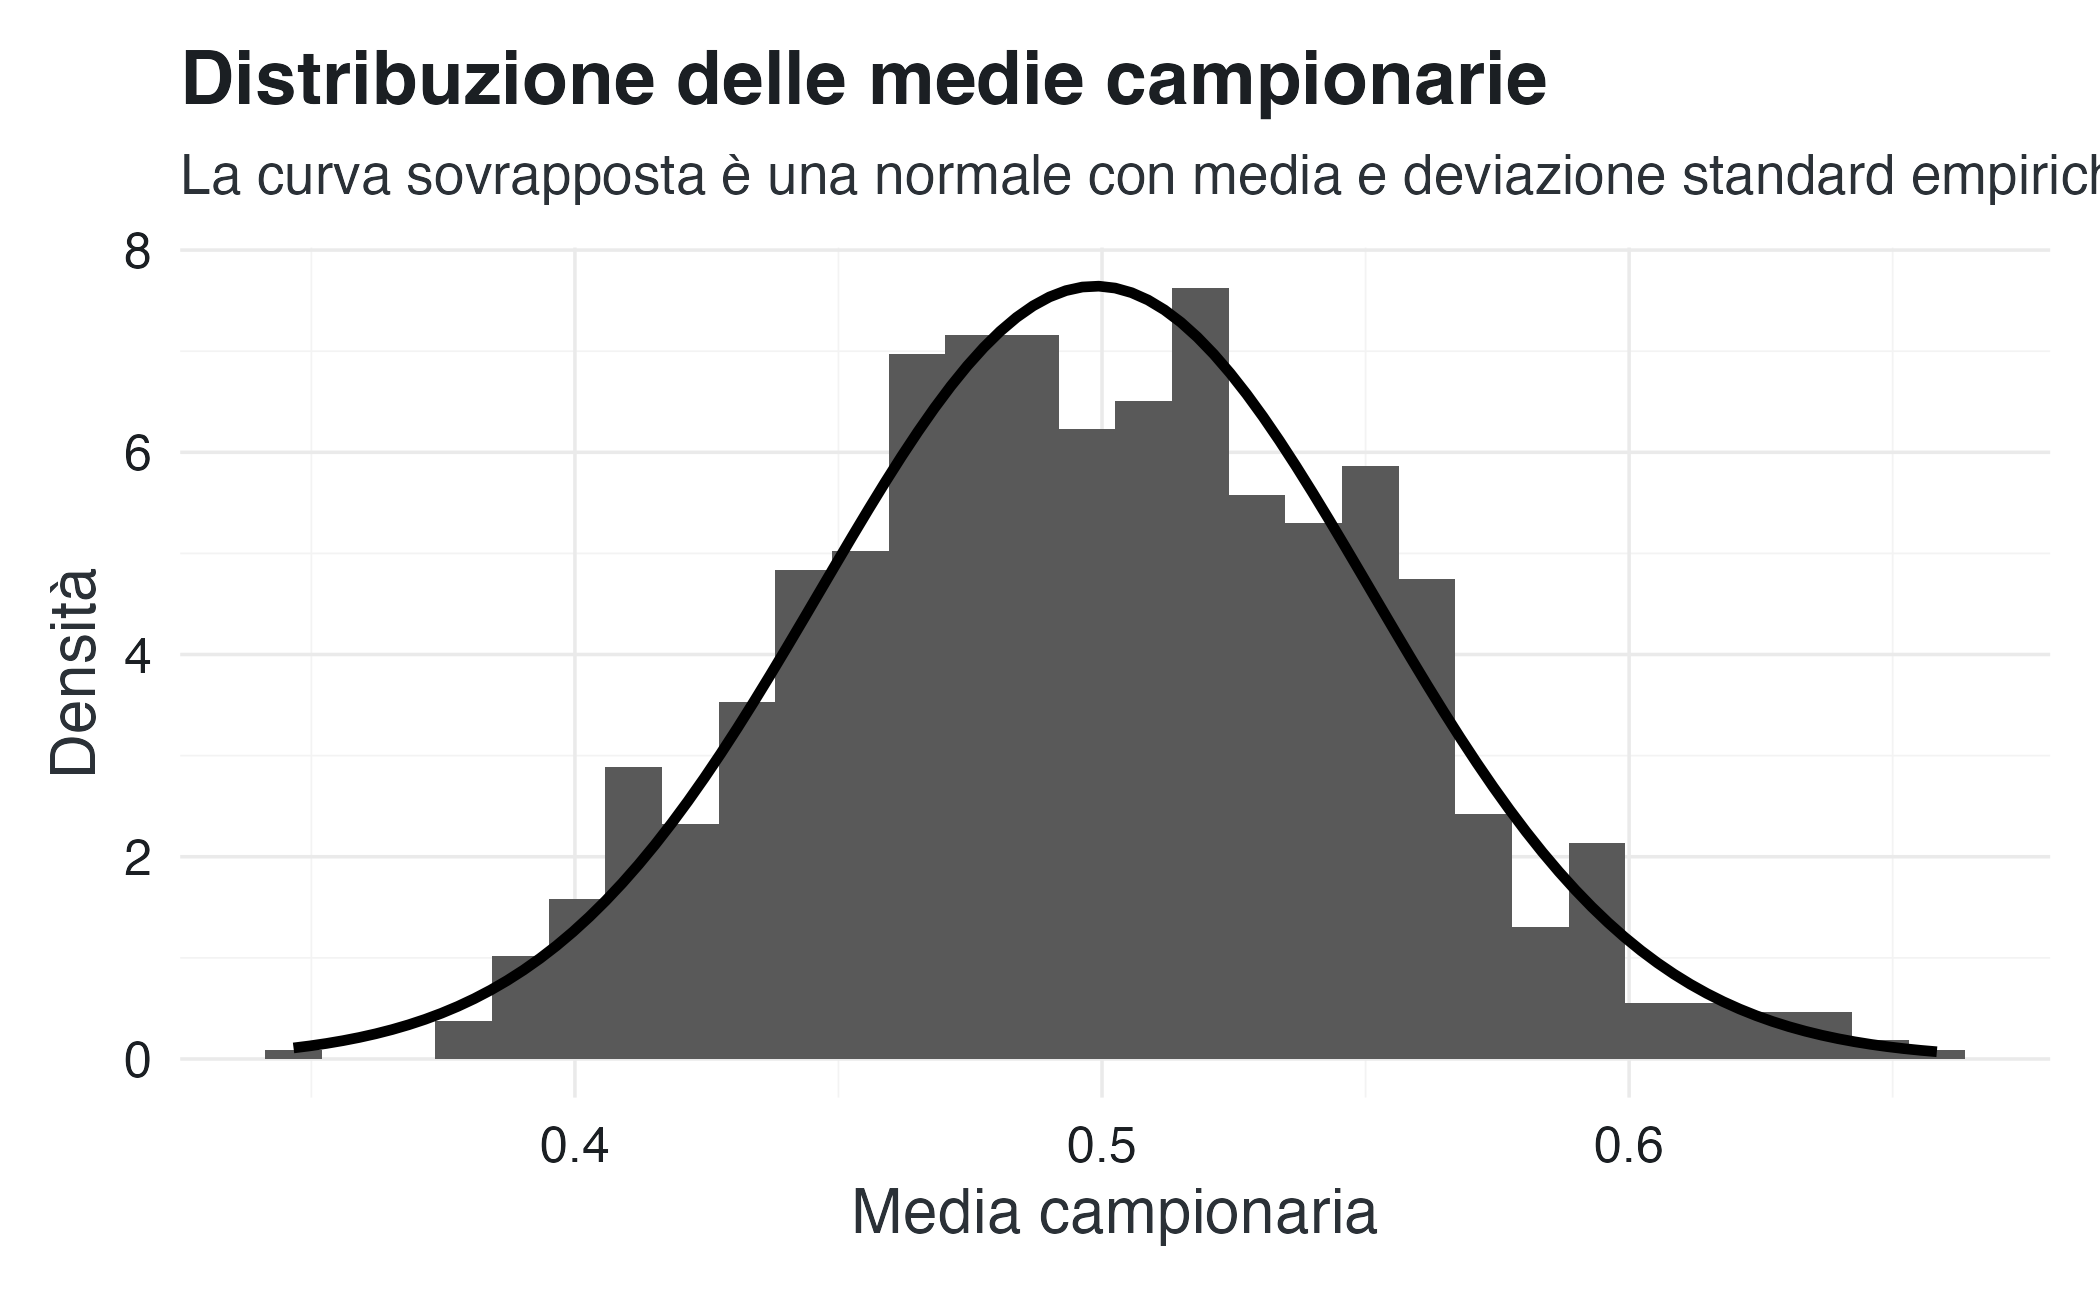
\includegraphics[width=0.85\linewidth,height=\textheight,keepaspectratio]{chapters/probability/13_from_sample_to_evidence_files/figure-pdf/clt-sampling-means-1.png}

}

\caption{Distribuzione delle medie campionarie: nonostante la
popolazione uniforme, le medie assumono una forma approssimativamente
normale.}

\end{figure}%

\subsection{Perché è importante per
l'inferenza}\label{perchuxe9-uxe8-importante-per-linferenza}

Il Teorema del Limite Centrale aiuta a capire perché molte procedure
inferenziali, anche bayesiane, assumono forme gaussiane quando i
campioni sono grandi. Se una statistica campionaria rilevante è
approssimativamente normale, allora anche l'evidenza prodotta dai dati
tende ad avere una forma regolare, concentrata e simmetrica attorno ai
valori più compatibili con le osservazioni.

Non si tratta di una licenza a usare sempre la normale, ma di una
spiegazione del perché l'approssimazione normale compaia così spesso
nella pratica.

\section{Prior, dati e sensibilità}\label{sec-prior-data-sensitivity}

\subsection{Il ruolo della prior in questa fase del
percorso}\label{il-ruolo-della-prior-in-questa-fase-del-percorso}

In questo capitolo non stiamo ancora calcolando posterior in modo
sistematico. Tuttavia, è utile ricordare la struttura generale
dell'aggiornamento bayesiano:

\[
p(\theta \mid D) \propto p(D \mid \theta) p(\theta).
\]

Il termine \(p(\theta)\) rappresenta le credenze prima dei dati; il
termine \(p(D \mid \theta)\) rappresenta quanto i dati sono compatibili
con ciascun valore del parametro. Il capitolo successivo sarà dedicato
proprio a formalizzare questo secondo termine come
\textbf{verosimiglianza}.

Qui ci interessa soprattutto l'intuizione: quando i dati sono pochi o
rumorosi, prior diverse possono produrre conclusioni diverse; quando i
dati sono molti e informativi, l'influenza della prior tende ad
attenuarsi, purché la prior non escluda in anticipo i valori compatibili
con i dati.

\subsection{Convergenza con prior
diverse}\label{convergenza-con-prior-diverse}

Consideriamo tre ricercatori con credenze iniziali diverse sulla
prevalenza \(\theta\):

\begin{itemize}
\tightlist
\item
  Ricercatore A: prior Beta(2, 8), centrata su valori bassi;
\item
  Ricercatore B: prior Beta(8, 2), centrata su valori alti;
\item
  Ricercatore C: prior Beta(1, 1), uniforme.
\end{itemize}

Supponiamo che i dati siano generati con \(\theta = 0.45\). Per diversi
valori di \(n\), osserviamo come cambiano le posterior Beta-Binomiale.

\begin{Shaded}
\begin{Highlighting}[]
\FunctionTok{set.seed}\NormalTok{(}\DecValTok{42}\NormalTok{)}
\NormalTok{theta\_true }\OtherTok{\textless{}{-}} \FloatTok{0.45}
\NormalTok{n\_osservazioni }\OtherTok{\textless{}{-}} \FunctionTok{c}\NormalTok{(}\DecValTok{10}\NormalTok{, }\DecValTok{50}\NormalTok{, }\DecValTok{200}\NormalTok{, }\DecValTok{1000}\NormalTok{)}

\NormalTok{definisci\_posterior }\OtherTok{\textless{}{-}} \ControlFlowTok{function}\NormalTok{(prior, n, theta) \{}
\NormalTok{  y }\OtherTok{\textless{}{-}} \FunctionTok{rbinom}\NormalTok{(}\DecValTok{1}\NormalTok{, n, theta)}
  \FunctionTok{c}\NormalTok{(}\AttributeTok{alpha =}\NormalTok{ prior[}\DecValTok{1}\NormalTok{] }\SpecialCharTok{+}\NormalTok{ y, }\AttributeTok{beta =}\NormalTok{ prior[}\DecValTok{2}\NormalTok{] }\SpecialCharTok{+}\NormalTok{ n }\SpecialCharTok{{-}}\NormalTok{ y)}
\NormalTok{\}}

\NormalTok{priors }\OtherTok{\textless{}{-}} \FunctionTok{list}\NormalTok{(}
  \StringTok{"A: prior bassa"} \OtherTok{=} \FunctionTok{c}\NormalTok{(}\DecValTok{2}\NormalTok{, }\DecValTok{8}\NormalTok{),}
  \StringTok{"B: prior alta"} \OtherTok{=} \FunctionTok{c}\NormalTok{(}\DecValTok{8}\NormalTok{, }\DecValTok{2}\NormalTok{),}
  \StringTok{"C: prior uniforme"} \OtherTok{=} \FunctionTok{c}\NormalTok{(}\DecValTok{1}\NormalTok{, }\DecValTok{1}\NormalTok{)}
\NormalTok{)}

\NormalTok{theta\_grid }\OtherTok{\textless{}{-}} \FunctionTok{seq}\NormalTok{(}\FloatTok{0.05}\NormalTok{, }\FloatTok{0.95}\NormalTok{, }\AttributeTok{length.out =} \DecValTok{500}\NormalTok{)}
\NormalTok{posterior\_plot }\OtherTok{\textless{}{-}} \FunctionTok{do.call}\NormalTok{(rbind, }\FunctionTok{lapply}\NormalTok{(n\_osservazioni, }\ControlFlowTok{function}\NormalTok{(n) \{}
  \FunctionTok{do.call}\NormalTok{(rbind, }\FunctionTok{lapply}\NormalTok{(}\FunctionTok{names}\NormalTok{(priors), }\ControlFlowTok{function}\NormalTok{(nome) \{}
\NormalTok{    post }\OtherTok{\textless{}{-}} \FunctionTok{definisci\_posterior}\NormalTok{(priors[[nome]], n, theta\_true)}
    \FunctionTok{data.frame}\NormalTok{(}
      \AttributeTok{theta =}\NormalTok{ theta\_grid,}
      \AttributeTok{density =} \FunctionTok{dbeta}\NormalTok{(theta\_grid, post[}\StringTok{"alpha"}\NormalTok{], post[}\StringTok{"beta"}\NormalTok{]),}
      \AttributeTok{prior =}\NormalTok{ nome,}
      \AttributeTok{n =} \FunctionTok{paste}\NormalTok{(}\StringTok{"n ="}\NormalTok{, n)}
\NormalTok{    )}
\NormalTok{  \}))}
\NormalTok{\}))}

\NormalTok{posterior\_plot}\SpecialCharTok{$}\NormalTok{n }\OtherTok{\textless{}{-}} \FunctionTok{factor}\NormalTok{(posterior\_plot}\SpecialCharTok{$}\NormalTok{n, }\AttributeTok{levels =} \FunctionTok{paste}\NormalTok{(}\StringTok{"n ="}\NormalTok{, n\_osservazioni))}

\FunctionTok{ggplot}\NormalTok{(posterior\_plot, }\FunctionTok{aes}\NormalTok{(}\AttributeTok{x =}\NormalTok{ theta, }\AttributeTok{y =}\NormalTok{ density, }\AttributeTok{linetype =}\NormalTok{ prior)) }\SpecialCharTok{+}
  \FunctionTok{geom\_line}\NormalTok{(}\AttributeTok{linewidth =} \FloatTok{1.1}\NormalTok{) }\SpecialCharTok{+}
  \FunctionTok{geom\_vline}\NormalTok{(}\AttributeTok{xintercept =}\NormalTok{ theta\_true, }\AttributeTok{linetype =} \StringTok{"dashed"}\NormalTok{, }\AttributeTok{linewidth =} \FloatTok{1.0}\NormalTok{) }\SpecialCharTok{+}
  \FunctionTok{facet\_wrap}\NormalTok{(}\SpecialCharTok{\textasciitilde{}}\NormalTok{ n, }\AttributeTok{ncol =} \DecValTok{2}\NormalTok{, }\AttributeTok{scales =} \StringTok{"free\_y"}\NormalTok{) }\SpecialCharTok{+}
  \FunctionTok{labs}\NormalTok{(}
    \AttributeTok{title =} \StringTok{"Da credenze diverse a conclusioni più simili"}\NormalTok{,}
    \AttributeTok{subtitle =} \StringTok{"La linea verticale indica il valore generativo theta = 0.45"}\NormalTok{,}
    \AttributeTok{x =} \StringTok{"Parametro theta"}\NormalTok{,}
    \AttributeTok{y =} \StringTok{"Densità a posteriori"}\NormalTok{,}
    \AttributeTok{linetype =} \StringTok{"Prior"}
\NormalTok{  ) }\SpecialCharTok{+}
  \FunctionTok{theme}\NormalTok{(}\AttributeTok{legend.position =} \StringTok{"bottom"}\NormalTok{)}
\end{Highlighting}
\end{Shaded}

\begin{figure}[H]

{\centering 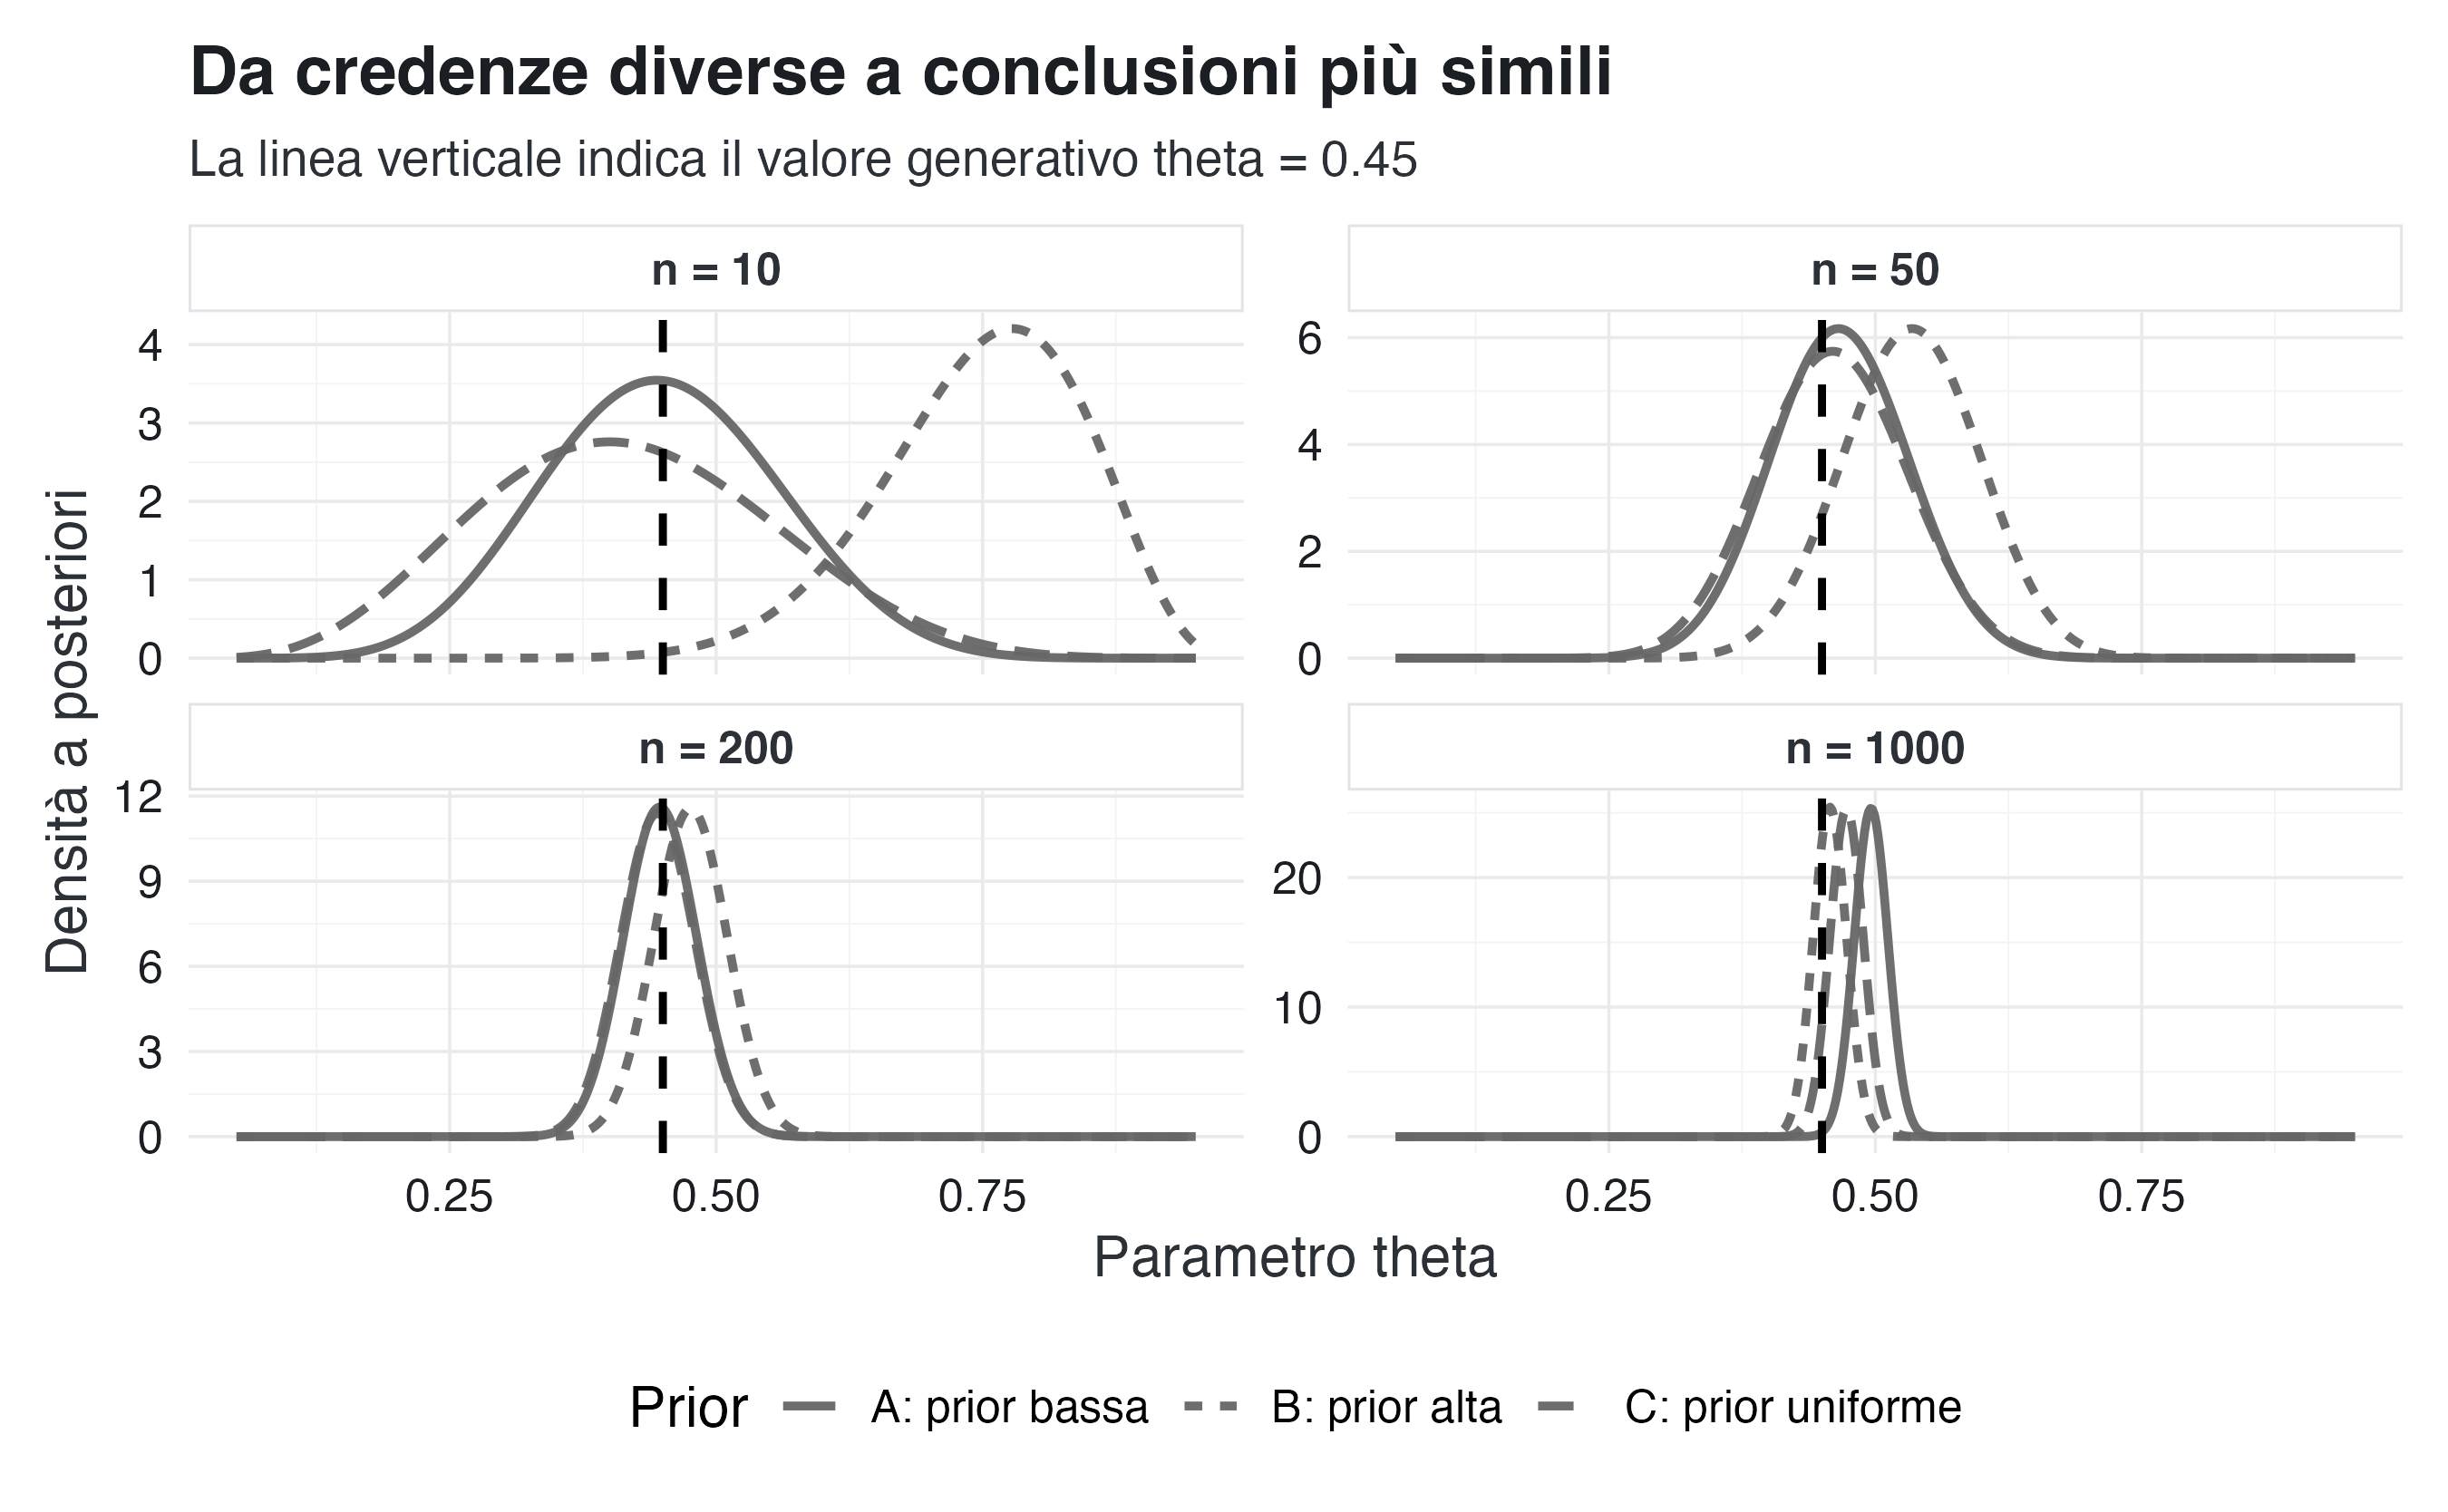
\includegraphics[width=1\linewidth,height=\textheight,keepaspectratio]{chapters/probability/13_from_sample_to_evidence_files/figure-pdf/bayesian-convergence-priors-1.png}

}

\caption{Convergenza delle distribuzioni posteriori con prior diverse al
crescere della dimensione campionaria.}

\end{figure}%

La simulazione mostra un messaggio importante: con pochi dati, le prior
contano molto; con molti dati, le differenze si riducono. Questo non
rende la prior irrilevante, ma chiarisce il suo ruolo: la prior è più
influente quando l'evidenza empirica è debole.

\subsection{Analisi di sensibilità}\label{analisi-di-sensibilituxe0}

L'\textbf{analisi di sensibilità} consiste nel verificare quanto le
conclusioni cambino al variare di assunzioni ragionevoli sulla prior. È
una pratica particolarmente importante nei contesti psicologici e
clinici, dove le conoscenze pregresse possono essere informative ma non
definitive.

\begin{Shaded}
\begin{Highlighting}[]
\NormalTok{n }\OtherTok{\textless{}{-}} \DecValTok{200}
\NormalTok{y }\OtherTok{\textless{}{-}} \DecValTok{90}

\NormalTok{priors\_sens }\OtherTok{\textless{}{-}} \FunctionTok{list}\NormalTok{(}
  \StringTok{"Informativa bassa"} \OtherTok{=} \FunctionTok{c}\NormalTok{(}\DecValTok{2}\NormalTok{, }\DecValTok{8}\NormalTok{),}
  \StringTok{"Uniforme"} \OtherTok{=} \FunctionTok{c}\NormalTok{(}\DecValTok{1}\NormalTok{, }\DecValTok{1}\NormalTok{),}
  \StringTok{"Informativa alta"} \OtherTok{=} \FunctionTok{c}\NormalTok{(}\DecValTok{8}\NormalTok{, }\DecValTok{2}\NormalTok{)}
\NormalTok{)}

\NormalTok{sens }\OtherTok{\textless{}{-}} \FunctionTok{do.call}\NormalTok{(rbind, }\FunctionTok{lapply}\NormalTok{(}\FunctionTok{names}\NormalTok{(priors\_sens), }\ControlFlowTok{function}\NormalTok{(nome) \{}
\NormalTok{  prior }\OtherTok{\textless{}{-}}\NormalTok{ priors\_sens[[nome]]}
\NormalTok{  post\_alpha }\OtherTok{\textless{}{-}}\NormalTok{ prior[}\DecValTok{1}\NormalTok{] }\SpecialCharTok{+}\NormalTok{ y}
\NormalTok{  post\_beta }\OtherTok{\textless{}{-}}\NormalTok{ prior[}\DecValTok{2}\NormalTok{] }\SpecialCharTok{+}\NormalTok{ n }\SpecialCharTok{{-}}\NormalTok{ y}
  \FunctionTok{data.frame}\NormalTok{(}
    \AttributeTok{prior =}\NormalTok{ nome,}
    \AttributeTok{media\_post =}\NormalTok{ post\_alpha }\SpecialCharTok{/}\NormalTok{ (post\_alpha }\SpecialCharTok{+}\NormalTok{ post\_beta),}
    \AttributeTok{q025 =} \FunctionTok{qbeta}\NormalTok{(}\FloatTok{0.025}\NormalTok{, post\_alpha, post\_beta),}
    \AttributeTok{q975 =} \FunctionTok{qbeta}\NormalTok{(}\FloatTok{0.975}\NormalTok{, post\_alpha, post\_beta)}
\NormalTok{  )}
\NormalTok{\}))}

\NormalTok{sens}
\CommentTok{\#\textgreater{}               prior media\_post  q025  q975}
\CommentTok{\#\textgreater{} 1 Informativa bassa      0.438 0.372 0.506}
\CommentTok{\#\textgreater{} 2          Uniforme      0.450 0.383 0.519}
\CommentTok{\#\textgreater{} 3  Informativa alta      0.467 0.400 0.534}
\end{Highlighting}
\end{Shaded}

Se le conclusioni sostantive sono simili per prior diverse, l'inferenza
è robusta. Se cambiano molto, il risultato non va nascosto: segnala che
i dati disponibili non sono ancora abbastanza informativi per superare
le differenze tra assunzioni iniziali plausibili.

\begin{tcolorbox}[enhanced jigsaw, arc=.35mm, bottomrule=.15mm, bottomtitle=1mm, breakable, colback=white, colbacktitle=quarto-callout-important-color!10!white, colframe=quarto-callout-important-color-frame, coltitle=black, left=2mm, leftrule=.75mm, opacityback=0, opacitybacktitle=0.6, rightrule=.15mm, title=\textcolor{quarto-callout-important-color}{\faExclamation}\hspace{0.5em}{Una buona pratica bayesiana}, titlerule=0mm, toprule=.15mm, toptitle=1mm]

La prior non è un fastidio da eliminare. È una parte esplicita del
modello. Proprio perché è esplicita, possiamo studiarne l'influenza con
analisi di sensibilità e comunicare quanto le conclusioni dipendano
dalle assunzioni iniziali.

\end{tcolorbox}

\section{Incertezza campionaria, bias e falsa
precisione}\label{sec-bias-false-precision}

\subsection{L'errore standard non misura
tutto}\label{lerrore-standard-non-misura-tutto}

L'errore standard quantifica la \textbf{variabilità campionaria}, ovvero
quanto una stima può fluttuare da un campione casuale all'altro sotto il
modello assunto. In termini bayesiani, misura l'incertezza epistemica
derivante dall'aver osservato solo una parte della popolazione.

Tuttavia, l'errore standard \textbf{non misura} gli errori sistematici
(\emph{bias}). Un campione molto ampio può produrre un errore standard
estremamente piccolo e, al tempo stesso, fornire una stima gravemente
distorta del parametro di interesse. La precisione statistica, ovvero un
intervallo di credibilità stretto, non garantisce l'accuratezza
scientifica.

Prendiamo un esempio concreto. Un'indagine online sul benessere
psicologico può raccogliere decine di migliaia di risposte, producendo
un errore standard dell'ordine di 0.005 (ovvero mezzo punto
percentuale). Se, però, il campione sovrarappresenta persone con accesso
a Internet, interesse per il tema o determinate caratteristiche
socio-demografiche, la stima può discostarsi dal valore vero nella
popolazione generale di 10 o 15 punti percentuali, un errore che non ha
nulla a che vedere con la variabilità campionaria.

\begin{tcolorbox}[enhanced jigsaw, arc=.35mm, bottomrule=.15mm, bottomtitle=1mm, breakable, colback=white, colbacktitle=quarto-callout-warning-color!10!white, colframe=quarto-callout-warning-color-frame, coltitle=black, left=2mm, leftrule=.75mm, opacityback=0, opacitybacktitle=0.6, rightrule=.15mm, title=\textcolor{quarto-callout-warning-color}{\faExclamationTriangle}\hspace{0.5em}{Il pericolo della falsa precisione}, titlerule=0mm, toprule=.15mm, toptitle=1mm]

La combinazione di un \textbf{errore standard piccolo} e un \textbf{bias
sostanziale} è la situazione più insidiosa: produce stime precise ma
sistematicamente errate, creando l'illusione di una conoscenza
affidabile.

Perciò, la qualità dell'inferenza non dipende solo dal numero di
osservazioni, ma anche dalla \textbf{validità del disegno di ricerca}:
rappresentatività del campione, accuratezza degli strumenti e assenza di
fonti di distorsione sistematica. Questi aspetti devono essere valutati
prima ancora di considerare l'errore standard.

\end{tcolorbox}

\subsection{Fonti comuni di bias nella ricerca
psicologica}\label{fonti-comuni-di-bias-nella-ricerca-psicologica}

Alcune fonti di distorsione particolarmente rilevanti sono:

\begin{itemize}
\tightlist
\item
  \textbf{bias di selezione}: il campione non rappresenta la popolazione
  di interesse;
\item
  \textbf{bias di risposta}: desiderabilità sociale, acquiescenza,
  stanchezza o motivazione differenziale;
\item
  \textbf{errore di misurazione}: lo strumento non misura adeguatamente
  il costrutto teorico;
\item
  \textbf{attrition selettiva}: abbandonano lo studio soprattutto alcuni
  tipi di partecipanti;
\item
  \textbf{specificazione incompleta del modello}: il modello ignora
  variabili o dipendenze rilevanti.
\end{itemize}

Questi problemi non scompaiono aumentando \(n\). Anzi, campioni molto
grandi possono rendere il problema più pericoloso, producendo intervalli
stretti attorno a un valore sbagliato.

\subsection{Precisione e accuratezza}\label{precisione-e-accuratezza}

\begin{figure}[H]

{\centering 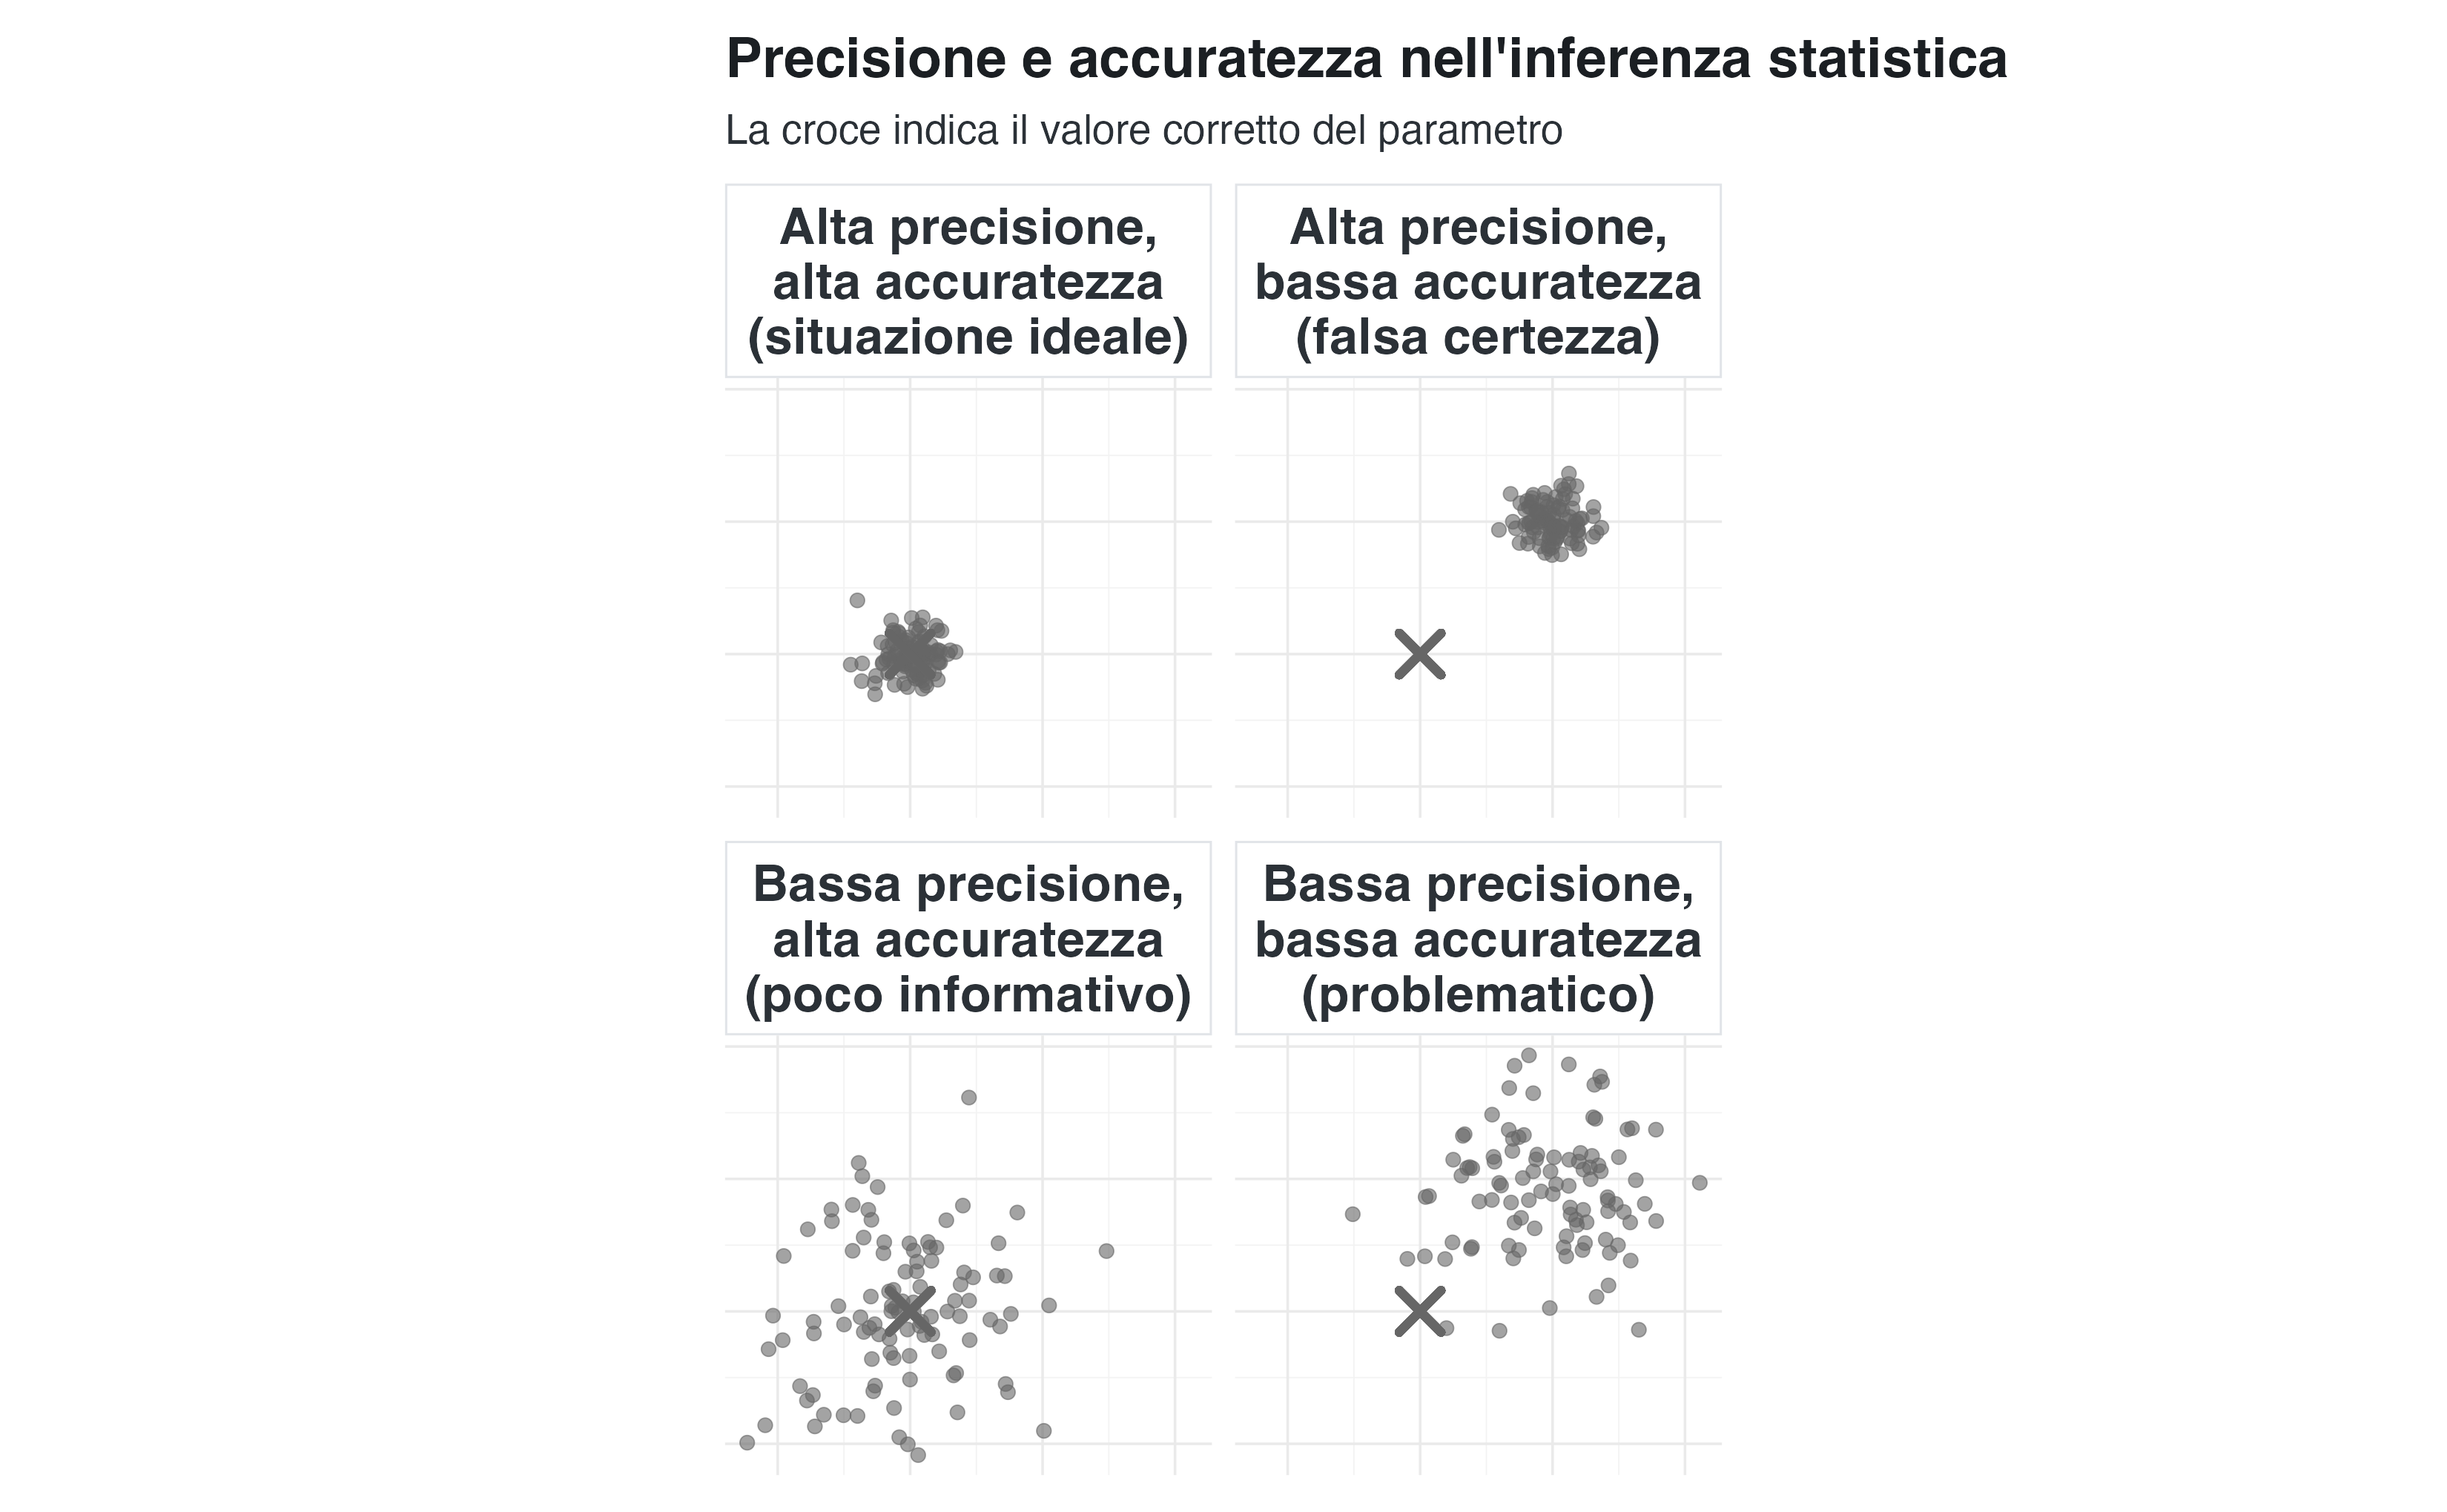
\includegraphics[width=1\linewidth,height=\textheight,keepaspectratio]{chapters/probability/13_from_sample_to_evidence_files/figure-pdf/precision-accuracy-plot-1.png}

}

\caption{Quattro combinazioni di precisione e accuratezza. Il centro
rappresenta il valore corretto del parametro.}

\end{figure}%

\begin{tcolorbox}[enhanced jigsaw, arc=.35mm, bottomrule=.15mm, bottomtitle=1mm, breakable, colback=white, colbacktitle=quarto-callout-warning-color!10!white, colframe=quarto-callout-warning-color-frame, coltitle=black, left=2mm, leftrule=.75mm, opacityback=0, opacitybacktitle=0.6, rightrule=.15mm, title=\textcolor{quarto-callout-warning-color}{\faExclamationTriangle}\hspace{0.5em}{Il pericolo della falsa precisione}, titlerule=0mm, toprule=.15mm, toptitle=1mm]

Un intervallo di credibilità stretto non garantisce che la conclusione
sia scientificamente valida. Garantisce solo che, date le assunzioni del
modello e i dati osservati, l'incertezza campionaria è ridotta.

Se il campione è distorto, la misura è inadeguata o il modello è mal
specificato, l'inferenza può essere molto precisa, ma anche molto
errata.

\end{tcolorbox}

\subsection{Come mitigare il problema}\label{come-mitigare-il-problema}

L'approccio bayesiano, se ben applicato, non elimina automaticamente le
distorsioni sistematiche, ma offre un vantaggio cruciale:
\textbf{costringe a renderle esplicite}. La trasparenza delle assunzioni
rappresenta già di per sé un argine contro l'illusione di oggettività. A
questa consapevolezza, si aggiungono alcune strategie operative:

\begin{enumerate}
\def\labelenumi{\arabic{enumi}.}
\item
  \textbf{Progettare lo studio con rigore prima ancora di raccogliere i
  dati}: la qualità dell'inferenza si gioca in larga parte nella fase di
  disegno, non in quella di analisi.
\item
  \textbf{Utilizzare strumenti di misura validati} e teoricamente
  coerenti con il costrutto di interesse, riducendo gli errori di
  misurazione sistematici.
\item
  \textbf{Modellare esplicitamente le fonti note di eterogeneità o
  distorsione}, quando possibile, includendole nel modello statistico
  piuttosto che ignorarle.
\item
  \textbf{Confrontare modelli alternativi} per valutare quanto le
  conclusioni dipendano dalla struttura specifica del modello adottato.
\item
  \textbf{Condurre analisi di sensibilità} sui prior e sulle assunzioni
  strutturali, verificando se le conclusioni cambiano sostanzialmente al
  variare di ipotesi ragionevoli.
\item
  \textbf{Distinguere sempre tra precisione statistica e validità
  sostantiva}: un intervallo di credibilità stretto non equivale a una
  stima corretta.
\end{enumerate}

In sintesi, l'inferenza bayesiana non rende i dati immuni dai bias, ma
rende il processo inferenziale più trasparente e, quindi, più facilmente
verificabile.

\section{Verso la verosimiglianza}\label{sec-towards-likelihood}

Abbiamo visto che un campione può essere più o meno informativo a
seconda della sua variabilità attesa. La media campionaria è centrata
sul valore generativo, la sua varianza diminuisce come \(\sigma^2/n\),
l'errore standard diminuisce come \(1/\sqrt{n}\) e, per molti problemi,
la sua distribuzione diventa approssimativamente normale.

Queste proprietà preparano la domanda centrale del prossimo capitolo:

\begin{quote}
Una volta osservati i dati, quali valori del parametro li rendono più
plausibili?
\end{quote}

La risposta è la \textbf{funzione di verosimiglianza}. Essa fissa i dati
osservati e valuta, per ogni valore possibile di \(\theta\), quanto quei
dati sarebbero attesi sotto il modello. In simboli, se il modello
specifica \(p(D \mid \theta)\), la verosimiglianza è la stessa
espressione letta come funzione di \(\theta\):

\[
L(\theta; D) = p(D \mid \theta).
\]

Nel Capitolo~\ref{sec-prob-likelihood} formalizzeremo questo cambio di
prospettiva: passeremo dalla domanda predittiva ``Quali dati potrei
osservare se \(\theta\) fosse noto?'' alla domanda inferenziale ``Quali
valori di \(\theta\) sono più compatibili con i dati osservati?''.

\section*{Riflessioni conclusive}\label{riflessioni-conclusive-12}

\markright{Riflessioni conclusive}

Questo capitolo ha chiarito il ruolo del campione come fonte di
evidenza. I dati non sono tutti ugualmente informativi: la loro forza
dipende dal modello, dalla dimensione campionaria, dalla variabilità
attesa e dalla qualità del disegno di ricerca.

Tre idee sono centrali:

\begin{enumerate}
\def\labelenumi{\arabic{enumi}.}
\tightlist
\item
  \textbf{La variabilità campionaria è quantificabile.} L'errore
  standard descrive quanto una statistica può fluttuare da un campione
  all'altro.
\item
  \textbf{L'informazione cresce con i dati, ma non magicamente.}
  Campioni più grandi aumentano la precisione, ma non correggono bias
  sistematici.
\item
  \textbf{L'inferenza bayesiana integra evidenza e credenze pregresse.}
  Quando i dati sono deboli, la prior conta di più; quando sono forti,
  l'evidenza tende a dominare, purché il modello sia adeguato.
\end{enumerate}

Il prossimo passo è formalizzare il modo in cui i dati discriminano tra
valori parametrici alternativi. Questo è il compito della
verosimiglianza.

\section*{Punti chiave da ricordare}\label{punti-chiave-da-ricordare-12}
\addcontentsline{toc}{section}{Punti chiave da ricordare}

\markright{Punti chiave da ricordare}

\begin{tcolorbox}[enhanced jigsaw, arc=.35mm, bottomrule=.15mm, bottomtitle=1mm, breakable, colback=white, colbacktitle=quarto-callout-important-color!10!white, colframe=quarto-callout-important-color-frame, coltitle=black, left=2mm, leftrule=.75mm, opacityback=0, opacitybacktitle=0.6, rightrule=.15mm, title=\textcolor{quarto-callout-important-color}{\faExclamation}\hspace{0.5em}{Importante}, titlerule=0mm, toprule=.15mm, toptitle=1mm]

\begin{enumerate}
\def\labelenumi{\arabic{enumi}.}
\tightlist
\item
  \textbf{Modello generativo}

  \begin{itemize}
  \tightlist
  \item
    Un modello collega parametri ignoti e dati osservabili.
  \item
    Nel caso Bernoulliano:
    \(X_i \mid \theta \sim \text{Bernoulli}(\theta)\).
  \end{itemize}
\item
  \textbf{Media o proporzione campionaria}

  \begin{itemize}
  \tightlist
  \item
    \(\mathbb{E}(\bar{X} \mid \theta)=\theta\).
  \item
    \(\text{Var}(\bar{X} \mid \theta)=\sigma^2/n\).
  \item
    Nel caso Bernoulliano:
    \(\text{SE}(\bar{X})=\sqrt{\theta(1-\theta)/n}\).
  \end{itemize}
\item
  \textbf{Distribuzione campionaria}

  \begin{itemize}
  \tightlist
  \item
    Descrive come una statistica varia da un campione all'altro.
  \item
    Aiuta a capire quanto il dato osservato sia informativo.
  \end{itemize}
\item
  \textbf{Precisione}

  \begin{itemize}
  \tightlist
  \item
    La precisione è l'inverso della varianza.
  \item
    Per la media campionaria cresce linearmente con \(n\).
  \item
    Le evidenze indipendenti si combinano naturalmente tramite le
    precisioni.
  \end{itemize}
\item
  \textbf{Legge dei Grandi Numeri}

  \begin{itemize}
  \tightlist
  \item
    La media campionaria converge al valore atteso.
  \item
    Spiega perché l'evidenza empirica si stabilizza con molti dati.
  \end{itemize}
\item
  \textbf{Teorema del Limite Centrale}

  \begin{itemize}
  \tightlist
  \item
    La media campionaria è spesso approssimativamente normale per \(n\)
    grande.
  \item
    Questo giustifica molte approssimazioni gaussiane nell'inferenza.
  \end{itemize}
\item
  \textbf{Sensibilità e bias}

  \begin{itemize}
  \tightlist
  \item
    Le prior diverse contano soprattutto quando i dati sono pochi.
  \item
    L'errore standard misura l'incertezza campionaria, non i bias
    sistematici.
  \item
    Precisione e accuratezza sono concetti distinti.
  \end{itemize}
\end{enumerate}

\textbf{Formule essenziali:}

\[
\mathbb{E}(\bar{X}) = \mu, \qquad
\text{Var}(\bar{X}) = \frac{\sigma^2}{n}, \qquad
\text{SE}(\bar{X}) = \frac{\sigma}{\sqrt{n}}.
\]

\[
\tau = \frac{1}{\text{Var}}, \qquad
\text{Precisione}(\bar{X}) = \frac{n}{\sigma^2}.
\]

\[
p(\theta \mid D) \propto p(D \mid \theta)p(\theta).
\]

\textbf{Per il prossimo capitolo:}

Nel Capitolo~\ref{sec-prob-likelihood} introdurremo la funzione di
verosimiglianza, cioè lo strumento che formalizza il modo in cui i dati
osservati rendono più o meno plausibili i diversi valori del parametro.

\end{tcolorbox}

\begin{tcolorbox}[enhanced jigsaw, arc=.35mm, bottomrule=.15mm, bottomtitle=1mm, breakable, colback=white, colbacktitle=quarto-callout-note-color!10!white, colframe=quarto-callout-note-color-frame, coltitle=black, left=2mm, leftrule=.75mm, opacityback=0, opacitybacktitle=0.6, rightrule=.15mm, title=\textcolor{quarto-callout-note-color}{\faInfo}\hspace{0.5em}{Informazioni sull'ambiente di sviluppo}, titlerule=0mm, toprule=.15mm, toptitle=1mm]

\begin{Shaded}
\begin{Highlighting}[]
\FunctionTok{sessionInfo}\NormalTok{()}
\CommentTok{\#\textgreater{} R version 4.6.1 (2026{-}06{-}24)}
\CommentTok{\#\textgreater{} Platform: aarch64{-}apple{-}darwin23}
\CommentTok{\#\textgreater{} Running under: macOS Tahoe 26.5.2}
\CommentTok{\#\textgreater{} }
\CommentTok{\#\textgreater{} Matrix products: default}
\CommentTok{\#\textgreater{} BLAS:   /Library/Frameworks/R.framework/Versions/4.6/Resources/lib/libRblas.0.dylib }
\CommentTok{\#\textgreater{} LAPACK: /Library/Frameworks/R.framework/Versions/4.6/Resources/lib/libRlapack.dylib;  LAPACK version 3.12.1}
\CommentTok{\#\textgreater{} }
\CommentTok{\#\textgreater{} locale:}
\CommentTok{\#\textgreater{} [1] C.UTF{-}8/UTF{-}8/C.UTF{-}8/C/C.UTF{-}8/C.UTF{-}8}
\CommentTok{\#\textgreater{} }
\CommentTok{\#\textgreater{} time zone: Europe/Rome}
\CommentTok{\#\textgreater{} tzcode source: internal}
\CommentTok{\#\textgreater{} }
\CommentTok{\#\textgreater{} attached base packages:}
\CommentTok{\#\textgreater{} [1] stats     graphics  grDevices utils     datasets  methods   base     }
\CommentTok{\#\textgreater{} }
\CommentTok{\#\textgreater{} other attached packages:}
\CommentTok{\#\textgreater{}  [1] ragg\_1.5.2            tinytable\_0.17.0      withr\_3.0.3          }
\CommentTok{\#\textgreater{}  [4] systemfonts\_1.3.2     patchwork\_1.3.2       ggdist\_3.3.3         }
\CommentTok{\#\textgreater{}  [7] tidybayes\_3.0.7       bayesplot\_1.15.0      ggplot2\_4.0.3        }
\CommentTok{\#\textgreater{} [10] reliabilitydiag\_0.2.1 priorsense\_1.2.0      posterior\_1.7.0      }
\CommentTok{\#\textgreater{} [13] loo\_2.10.0            rstan\_2.32.7          StanHeaders\_2.32.10  }
\CommentTok{\#\textgreater{} [16] brms\_2.23.0           Rcpp\_1.1.2            sessioninfo\_1.2.4    }
\CommentTok{\#\textgreater{} [19] conflicted\_1.2.0      janitor\_2.2.1         matrixStats\_1.5.0    }
\CommentTok{\#\textgreater{} [22] modelr\_0.1.11         tibble\_3.3.1          dplyr\_1.2.1          }
\CommentTok{\#\textgreater{} [25] tidyr\_1.3.2           rio\_1.3.0             here\_1.0.2           }
\CommentTok{\#\textgreater{} }
\CommentTok{\#\textgreater{} loaded via a namespace (and not attached):}
\CommentTok{\#\textgreater{}  [1] svUnit\_1.0.8          tidyselect\_1.2.1      farver\_2.1.2         }
\CommentTok{\#\textgreater{}  [4] S7\_0.2.2              fastmap\_1.2.0         tensorA\_0.36.2.1     }
\CommentTok{\#\textgreater{}  [7] digest\_0.6.39         timechange\_0.4.0      estimability\_2.0.0   }
\CommentTok{\#\textgreater{} [10] lifecycle\_1.0.5       magrittr\_2.0.5        compiler\_4.6.1       }
\CommentTok{\#\textgreater{} [13] rlang\_1.3.0           tools\_4.6.1           yaml\_2.3.12          }
\CommentTok{\#\textgreater{} [16] knitr\_1.51            labeling\_0.4.3        bridgesampling\_1.2{-}1 }
\CommentTok{\#\textgreater{} [19] pkgbuild\_1.4.8        curl\_7.1.0            RColorBrewer\_1.1{-}3   }
\CommentTok{\#\textgreater{} [22] abind\_1.4{-}8           purrr\_1.2.2           grid\_4.6.1           }
\CommentTok{\#\textgreater{} [25] stats4\_4.6.1          xtable\_1.8{-}8          inline\_0.3.21        }
\CommentTok{\#\textgreater{} [28] emmeans\_2.0.3         scales\_1.4.0          cli\_3.6.6            }
\CommentTok{\#\textgreater{} [31] mvtnorm\_1.4{-}1         rmarkdown\_2.31        generics\_0.1.4       }
\CommentTok{\#\textgreater{} [34] otel\_0.2.0            RcppParallel\_5.1.11{-}2 cachem\_1.1.0         }
\CommentTok{\#\textgreater{} [37] stringr\_1.6.0         parallel\_4.6.1        vctrs\_0.7.3          }
\CommentTok{\#\textgreater{} [40] V8\_8.2.0              Matrix\_1.7{-}5          jsonlite\_2.0.0       }
\CommentTok{\#\textgreater{} [43] arrayhelpers\_1.1{-}1    glue\_1.8.1            codetools\_0.2{-}20     }
\CommentTok{\#\textgreater{} [46] distributional\_0.8.1  lubridate\_1.9.5       stringi\_1.8.7        }
\CommentTok{\#\textgreater{} [49] gtable\_0.3.6          QuickJSR\_1.10.0       pillar\_1.11.1        }
\CommentTok{\#\textgreater{} [52] htmltools\_0.5.9       Brobdingnag\_1.2{-}9     R6\_2.6.1             }
\CommentTok{\#\textgreater{} [55] textshaping\_1.0.5     rprojroot\_2.1.1       evaluate\_1.0.5       }
\CommentTok{\#\textgreater{} [58] lattice\_0.22{-}9        backports\_1.5.1       memoise\_2.0.1        }
\CommentTok{\#\textgreater{} [61] broom\_1.0.13          snakecase\_0.11.1      rstantools\_2.6.0     }
\CommentTok{\#\textgreater{} [64] coda\_0.19{-}4.1         gridExtra\_2.3.1       nlme\_3.1{-}169         }
\CommentTok{\#\textgreater{} [67] checkmate\_2.3.4       xfun\_0.60             pkgconfig\_2.0.3}
\end{Highlighting}
\end{Shaded}

\end{tcolorbox}

\section*{Bibliografia}\label{bibliografia-7}

\markright{Bibliografia}

\chapter{La verosimiglianza}\label{sec-prob-likelihood}

\section*{Introduzione}\label{introduzione-13}

\markright{Introduzione}

Nel capitolo precedente abbiamo studiato il campione come fonte di
evidenza. Abbiamo visto che una proporzione osservata, una media
campionaria o un'altra statistica non sono informative di per sé:
diventano informative solo in relazione di un modello probabilistico che
collega i dati osservabili ai parametri sconosciuti.

Ora facciamo il passo successivo. Supponiamo, per esempio, di osservare
che in uno studio pilota il 36\% dei pazienti trattati raggiunge la
remissione completa: possiamo chiederci quali valori dell'efficacia
reale del trattamento rendono più plausibile un risultato di questo
tipo. Un'efficacia del 20\% è compatibile con i dati? E una del 40\%? E
una del 60\%?

La \textbf{funzione di verosimiglianza} serve proprio a questo:
trasforma i dati osservati in una mappa di compatibilità per i valori
possibili del parametro. La funzione di verosimiglianza non assegna
ancora probabilità ai parametri, questo compito spetta alla
distribuzione a posteriori, ma ci dice quanto i dati siano plausibili
sotto ciascun valore del parametro.

La domanda guida del capitolo è quindi:

\begin{quote}
Avendo osservato questi dati, quali valori del parametro li rendono più
o meno plausibili?
\end{quote}

In questo capitolo:

\begin{enumerate}
\def\labelenumi{\arabic{enumi}.}
\tightlist
\item
  \textbf{distingueremo} chiaramente probabilità predittiva e
  verosimiglianza;
\item
  \textbf{definiremo} formalmente la funzione di verosimiglianza;
\item
  \textbf{mostreremo} perché la verosimiglianza non è una distribuzione
  di probabilità sui parametri;
\item
  \textbf{useremo} il modello Bernoulli--binomiale per costruire e
  interpretare una verosimiglianza;
\item
  \textbf{introdurremo} la log-verosimiglianza come strumento
  computazionale e concettuale;
\item
  \textbf{discuteremo} la verosimiglianza congiunta per osservazioni
  multiple e per studi indipendenti;
\item
  \textbf{esamineremo} il caso gaussiano, collegandolo alla precisione
  discussa nel capitolo precedente;
\item
  \textbf{chiariremo} il ruolo, utile ma limitato, della massima
  verosimiglianza;
\item
  \textbf{chiuderemo} collegando la verosimiglianza all'aggiornamento
  bayesiano del capitolo successivo.
\end{enumerate}

\begin{tcolorbox}[enhanced jigsaw, arc=.35mm, bottomrule=.15mm, bottomtitle=1mm, breakable, colback=white, colbacktitle=quarto-callout-tip-color!10!white, colframe=quarto-callout-tip-color-frame, coltitle=black, left=2mm, leftrule=.75mm, opacityback=0, opacitybacktitle=0.6, rightrule=.15mm, title=\textcolor{quarto-callout-tip-color}{\faLightbulb}\hspace{0.5em}{Prerequisiti}, titlerule=0mm, toprule=.15mm, toptitle=1mm]

Per seguire questo capitolo è utile aver letto:

\begin{itemize}
\tightlist
\item
  Capitolo~\ref{sec-prob-bayes-theorem} --- per la struttura generale
  dell'aggiornamento bayesiano;
\item
  Capitolo~\ref{sec-prob-inference-uncertainty} --- per il ruolo
  dell'evidenza, dell'errore standard e della precisione;
\item
  1 --- per il linguaggio delle distribuzioni parametriche;
\item
  2 --- per Bernoulli e Binomiale;
\item
  Capitolo~\ref{sec-prob-cont-distr} --- per la distribuzione Normale.
\end{itemize}

Questo capitolo formalizza il collegamento tra dati e parametri: la
verosimiglianza è il modo in cui i dati entrano nel teorema di Bayes.

\end{tcolorbox}

\begin{tcolorbox}[enhanced jigsaw, arc=.35mm, bottomrule=.15mm, bottomtitle=1mm, breakable, colback=white, colbacktitle=quarto-callout-caution-color!10!white, colframe=quarto-callout-caution-color-frame, coltitle=black, left=2mm, leftrule=.75mm, opacityback=0, opacitybacktitle=0.6, rightrule=.15mm, title=\textcolor{quarto-callout-caution-color}{\faFire}\hspace{0.5em}{Preparazione del Notebook}, titlerule=0mm, toprule=.15mm, toptitle=1mm]

\begin{Shaded}
\begin{Highlighting}[]
\NormalTok{here}\SpecialCharTok{::}\FunctionTok{here}\NormalTok{(}\StringTok{"code"}\NormalTok{, }\StringTok{"\_common.R"}\NormalTok{) }\SpecialCharTok{|\textgreater{}} 
  \FunctionTok{source}\NormalTok{()}

\CommentTok{\# Riapplica il tema per sicurezza}
\FunctionTok{apply\_visual\_theme}\NormalTok{()}
\end{Highlighting}
\end{Shaded}

\end{tcolorbox}

\section{Dal modello generativo alla domanda
inversa}\label{sec-likelihood-inverse-question}

\subsection{La direzione predittiva}\label{la-direzione-predittiva}

Un modello probabilistico specifica come potrebbero essere generati i
dati se il valore del parametro fosse noto. Nel caso di osservazioni
binarie, possiamo scrivere:

\[
Y_i \mid \theta \sim \text{Bernoulli}(\theta), \qquad i = 1, \ldots, n.
\]

Se \(\theta = 0.36\), il modello dice che ogni osservazione ha
probabilità 0.36 di essere un successo. Questa è la direzione
\textbf{predittiva} del modello:

\[
\theta \quad \longrightarrow \quad \text{dati possibili}.
\]

In questa direzione, il parametro è fissato e i dati sono incerti.
Possiamo quindi calcolare probabilità del tipo:

\[
p(y \mid \theta).
\]

Questa quantità risponde alla domanda:

\begin{quote}
Se il parametro avesse valore \(\theta\), quali dati potremmo osservare
e con quale probabilità?
\end{quote}

\subsection{La direzione inferenziale}\label{la-direzione-inferenziale}

Nella ricerca empirica, però, di solito ci troviamo nella situazione
opposta: i dati sono già stati osservati, mentre il parametro è ignoto.
Se osserviamo \(y = 72\) remissioni su \(n = 200\) pazienti, la domanda
non è più ``quali dati potremmo osservare?'', ma:

\begin{quote}
Quali valori di \(\theta\) rendono plausibile osservare 72 remissioni su
200 pazienti?
\end{quote}

Questa è la direzione \textbf{inferenziale}:

\[
\text{dati osservati} \quad \longrightarrow \quad \text{valori plausibili del parametro}.
\]

La verosimiglianza nasce da questo cambio di prospettiva.

\begin{tcolorbox}[enhanced jigsaw, arc=.35mm, bottomrule=.15mm, bottomtitle=1mm, breakable, colback=white, colbacktitle=quarto-callout-note-color!10!white, colframe=quarto-callout-note-color-frame, coltitle=black, left=2mm, leftrule=.75mm, opacityback=0, opacitybacktitle=0.6, rightrule=.15mm, title=\textcolor{quarto-callout-note-color}{\faInfo}\hspace{0.5em}{Idea chiave}, titlerule=0mm, toprule=.15mm, toptitle=1mm]

La funzione matematica \(p(y \mid \theta)\) è la stessa, ma cambia ciò
che consideriamo fisso e ciò che consideriamo variabile. Come
probabilità, varia \(y\) e \(\theta\) è fissato. Come verosimiglianza,
\(y\) è fissato e varia \(\theta\).

\end{tcolorbox}

\section{Definizione di funzione di
verosimiglianza}\label{sec-likelihood-definition}

\begin{definition}[Funzione di
verosimiglianza]\protect\hypertarget{def-likelihood}{}\label{def-likelihood}

Sia \(Y\) una variabile casuale, o un vettore di variabili casuali, la
cui distribuzione dipende da un parametro ignoto \(\theta \in \Theta\).
Indichiamo con \(f(y \mid \theta)\) la funzione di massa di probabilità,
nel caso discreto, o la funzione di densità, nel caso continuo.

Una volta osservati i dati \(y_{obs}\), la \textbf{funzione di
verosimiglianza} è:

\[
L(\theta; y_{obs}) = f(y_{obs} \mid \theta), \qquad \theta \in \Theta.
\]

Nella verosimiglianza:

\begin{itemize}
\tightlist
\item
  \(y_{obs}\) è fissato: rappresenta ciò che abbiamo osservato;
\item
  \(\theta\) varia: rappresenta i valori parametrici che vogliamo
  confrontare.
\end{itemize}

\end{definition}

La verosimiglianza misura quanto i dati osservati siano compatibili con
ciascun valore del parametro. Valori di \(\theta\) che assegnano
maggiore probabilità o densità ai dati osservati hanno verosimiglianza
maggiore.

Questa frase richiede attenzione: \textbf{la verosimiglianza non è la
probabilità che \(\theta\) sia vero}. Essa dice invece quanto sarebbero
plausibili i dati se \(\theta\) avesse un certo valore.

\subsection{Probabilità e verosimiglianza a
confronto}\label{probabilituxe0-e-verosimiglianza-a-confronto}

{\def\LTcaptype{none} % do not increment counter
\begin{longtable}[]{@{}
  >{\raggedright\arraybackslash}p{(\linewidth - 4\tabcolsep) * \real{0.3333}}
  >{\raggedright\arraybackslash}p{(\linewidth - 4\tabcolsep) * \real{0.3333}}
  >{\raggedright\arraybackslash}p{(\linewidth - 4\tabcolsep) * \real{0.3333}}@{}}
\toprule\noalign{}
\begin{minipage}[b]{\linewidth}\raggedright
Aspetto
\end{minipage} & \begin{minipage}[b]{\linewidth}\raggedright
Probabilità / densità
\end{minipage} & \begin{minipage}[b]{\linewidth}\raggedright
Verosimiglianza
\end{minipage} \\
\midrule\noalign{}
\endhead
\bottomrule\noalign{}
\endlastfoot
Espressione & \(f(y \mid \theta)\) &
\(L(\theta; y_{obs}) = f(y_{obs} \mid \theta)\) \\
Quantità fissata & \(\theta\) & \(y_{obs}\) \\
Quantità variabile & \(y\) & \(\theta\) \\
Domanda & Quali dati posso osservare se conosco \(\theta\)? & Quali
valori di \(\theta\) rendono plausibili i dati osservati? \\
Uso principale & Predizione & Inferenza \\
Normalizzazione & Somma/integra a 1 rispetto a \(y\) & In generale non
somma/integra a 1 rispetto a \(\theta\) \\
\end{longtable}
}

\subsection{Perché non è una distribuzione sui
parametri}\label{perchuxe9-non-uxe8-una-distribuzione-sui-parametri}

La verosimiglianza è una funzione di \(\theta\), ma non è
automaticamente una distribuzione di probabilità su \(\theta\). In
generale:

\[
\int_\Theta L(\theta; y_{obs})\,d\theta \neq 1.
\]

Nel caso discreto, analogamente:

\[
\sum_{\theta \in \Theta} L(\theta; y_{obs}) \neq 1.
\]

Questo è un punto essenziale per la prospettiva bayesiana. Per ottenere
una distribuzione sui parametri occorre combinare la verosimiglianza con
una distribuzione a priori e poi normalizzare:

\[
p(\theta \mid y_{obs})
= \frac{L(\theta; y_{obs})p(\theta)}{\int L(\theta'; y_{obs})p(\theta')\,d\theta'}.
\]

Il capitolo successivo sarà dedicato proprio a questo passaggio.

\begin{tcolorbox}[enhanced jigsaw, arc=.35mm, bottomrule=.15mm, bottomtitle=1mm, breakable, colback=white, colbacktitle=quarto-callout-important-color!10!white, colframe=quarto-callout-important-color-frame, coltitle=black, left=2mm, leftrule=.75mm, opacityback=0, opacitybacktitle=0.6, rightrule=.15mm, title=\textcolor{quarto-callout-important-color}{\faExclamation}\hspace{0.5em}{Da ricordare}, titlerule=0mm, toprule=.15mm, toptitle=1mm]

La verosimiglianza è il contributo dei dati all'aggiornamento bayesiano.
Non è ancora una credenza aggiornata: diventa parte della distribuzione
a posteriori solo quando viene combinata con la prior.

\end{tcolorbox}

\section{Scala arbitraria e verosimiglianza
relativa}\label{sec-relative-likelihood}

La scala assoluta della verosimiglianza spesso non è importante. Per
confrontare valori diversi dello stesso parametro, ciò che conta sono i
\textbf{rapporti} tra verosimiglianze.

Se due funzioni differiscono solo per una costante positiva che non
dipende da \(\theta\),

\[
L_1(\theta) = c L_2(\theta), \qquad c > 0,
\]

allora forniscono la stessa informazione sui valori relativi di
\(\theta\). Infatti:

\[
\frac{L_1(\theta_a)}{L_1(\theta_b)}
= \frac{cL_2(\theta_a)}{cL_2(\theta_b)}
= \frac{L_2(\theta_a)}{L_2(\theta_b)}.
\]

Per questo motivo, quando lavoriamo con la verosimiglianza scriviamo
spesso:

\[
L(\theta; y) \propto f(y \mid \theta),
\]

intendendo che abbiamo eliminato costanti che non dipendono da
\(\theta\).

\subsection{La verosimiglianza
relativa}\label{la-verosimiglianza-relativa}

Per rendere più interpretabile una curva di verosimiglianza, possiamo
dividerla per il suo valore massimo:

\[
R(\theta) = \frac{L(\theta)}{\max_{\theta'} L(\theta')}.
\]

La funzione \(R(\theta)\) prende valori tra 0 e 1. Il valore 1
corrisponde al parametro più supportato dai dati, mentre valori più
bassi indicano supporto relativo minore.

\begin{tcolorbox}[enhanced jigsaw, arc=.35mm, bottomrule=.15mm, bottomtitle=1mm, breakable, colback=white, colbacktitle=quarto-callout-note-color!10!white, colframe=quarto-callout-note-color-frame, coltitle=black, left=2mm, leftrule=.75mm, opacityback=0, opacitybacktitle=0.6, rightrule=.15mm, title=\textcolor{quarto-callout-note-color}{\faInfo}\hspace{0.5em}{Interpretazione prudente}, titlerule=0mm, toprule=.15mm, toptitle=1mm]

Dire che \(R(\theta)=0.5\) non significa che \(\theta\) abbia
probabilità 50\%. Significa che quel valore rende i dati plausibili la
metà rispetto al valore che massimizza la verosimiglianza.

\end{tcolorbox}

\section{Verosimiglianza
Bernoulli--binomiale}\label{sec-binomial-likelihood}

\subsection{Dati individuali
Bernoulliani}\label{dati-individuali-bernoulliani}

Supponiamo di osservare \(n\) risposte binarie:

\[
y_i =
\begin{cases}
1 & \text{se il paziente raggiunge la remissione}, \\
0 & \text{altrimenti}.
\end{cases}
\]

Assumiamo:

\[
Y_i \mid \theta \sim \text{Bernoulli}(\theta),
\]

dove \(\theta\) è la probabilità di remissione.

Per una singola osservazione, la probabilità del dato osservato è:

\[
p(y_i \mid \theta) = \theta^{y_i}(1-\theta)^{1-y_i}.
\]

Se le osservazioni sono indipendenti, la verosimiglianza congiunta è:

\[
L(\theta; y_1, \ldots, y_n)
= \prod_{i=1}^{n} \theta^{y_i}(1-\theta)^{1-y_i}.
\]

Raccogliendo i termini, otteniamo:

\[
L(\theta; y_1, \ldots, y_n)
= \theta^{\sum_i y_i}(1-\theta)^{n-\sum_i y_i}.
\]

Se indichiamo con

\[
y = \sum_{i=1}^{n} y_i
\]

il numero totale di successi, allora:

\[
L(\theta; y, n) \propto \theta^y(1-\theta)^{n-y}.
\]

Questo risultato mostra che, nel modello Bernoulli indipendente,
l'ordine delle osservazioni non aggiunge informazione su \(\theta\):
conta il numero totale di successi.

\subsection{La forma binomiale}\label{la-forma-binomiale}

Se osserviamo direttamente il numero totale di successi \(Y=y\) su \(n\)
prove, allora:

\[
Y \mid \theta \sim \text{Binomiale}(n, \theta),
\]

e quindi:

\[
p(y \mid \theta) = {n \choose y}\theta^y(1-\theta)^{n-y}.
\]

Vista come funzione di \(\theta\), questa diventa:

\[
L(\theta; y,n) = {n \choose y}\theta^y(1-\theta)^{n-y}.
\]

Il coefficiente combinatorio \({n \choose y}\) non dipende da
\(\theta\), quindi per confrontare valori di \(\theta\) possiamo usare
la forma proporzionale:

\[
L(\theta; y,n) \propto \theta^y(1-\theta)^{n-y}.
\]

\begin{tcolorbox}[enhanced jigsaw, arc=.35mm, bottomrule=.15mm, bottomtitle=1mm, breakable, colback=white, colbacktitle=quarto-callout-note-color!10!white, colframe=quarto-callout-note-color-frame, coltitle=black, left=2mm, leftrule=.75mm, opacityback=0, opacitybacktitle=0.6, rightrule=.15mm, title=\textcolor{quarto-callout-note-color}{\faInfo}\hspace{0.5em}{Una costante può essere ignorata?}, titlerule=0mm, toprule=.15mm, toptitle=1mm]

Se l'obiettivo è confrontare valori diversi dello stesso parametro nello
stesso modello, le costanti che non dipendono da \(\theta\) possono
essere ignorate. Se invece si confrontano modelli diversi tramite
probabilità marginali, le costanti devono essere gestite con maggiore
attenzione.

\end{tcolorbox}

\section{Un esempio psicologico: remissione in uno studio
pilota}\label{sec-likelihood-remission-example}

Riprendiamo l'esempio del trattamento clinico. Supponiamo di osservare
\(y=72\) remissioni su \(n=200\) pazienti. La proporzione campionaria è:

\[
\hat{\theta} = \frac{72}{200} = 0.36.
\]

La verosimiglianza binomiale è:

\[
L(\theta; y=72,n=200) \propto \theta^{72}(1-\theta)^{128}.
\]

Questa funzione assegna il supporto massimo a \(\theta=0.36\), ma non
esclude in modo assoluto valori vicini, come 0.34 o 0.39. Li rende solo
meno supportati in base alla loro capacità di rendere plausibile il dato
osservato.

\begin{Shaded}
\begin{Highlighting}[]
\NormalTok{n }\OtherTok{\textless{}{-}} \DecValTok{200}
\NormalTok{y }\OtherTok{\textless{}{-}} \DecValTok{72}
\NormalTok{theta\_grid }\OtherTok{\textless{}{-}} \FunctionTok{seq}\NormalTok{(}\FloatTok{0.001}\NormalTok{, }\FloatTok{0.999}\NormalTok{, }\AttributeTok{length.out =} \DecValTok{1000}\NormalTok{)}
\NormalTok{log\_lik }\OtherTok{\textless{}{-}} \FunctionTok{dbinom}\NormalTok{(y, }\AttributeTok{size =}\NormalTok{ n, }\AttributeTok{prob =}\NormalTok{ theta\_grid, }\AttributeTok{log =} \ConstantTok{TRUE}\NormalTok{)}
\NormalTok{rel\_lik }\OtherTok{\textless{}{-}} \FunctionTok{exp}\NormalTok{(log\_lik }\SpecialCharTok{{-}} \FunctionTok{max}\NormalTok{(log\_lik))}

\NormalTok{df\_lik }\OtherTok{\textless{}{-}} \FunctionTok{data.frame}\NormalTok{(}
  \AttributeTok{theta =}\NormalTok{ theta\_grid,}
  \AttributeTok{relative\_likelihood =}\NormalTok{ rel\_lik}
\NormalTok{)}

\FunctionTok{ggplot}\NormalTok{(df\_lik, }\FunctionTok{aes}\NormalTok{(}\AttributeTok{x =}\NormalTok{ theta, }\AttributeTok{y =}\NormalTok{ relative\_likelihood)) }\SpecialCharTok{+}
  \FunctionTok{geom\_line}\NormalTok{(}\AttributeTok{linewidth =} \FloatTok{1.2}\NormalTok{) }\SpecialCharTok{+}
  \FunctionTok{geom\_vline}\NormalTok{(}\AttributeTok{xintercept =}\NormalTok{ y }\SpecialCharTok{/}\NormalTok{ n, }\AttributeTok{linetype =} \StringTok{"dashed"}\NormalTok{) }\SpecialCharTok{+}
  \FunctionTok{labs}\NormalTok{(}
    \AttributeTok{x =} \FunctionTok{expression}\NormalTok{(theta),}
    \AttributeTok{y =} \StringTok{"Verosimiglianza relativa"}
\NormalTok{  )}
\end{Highlighting}
\end{Shaded}

\begin{figure}[H]

\centering{

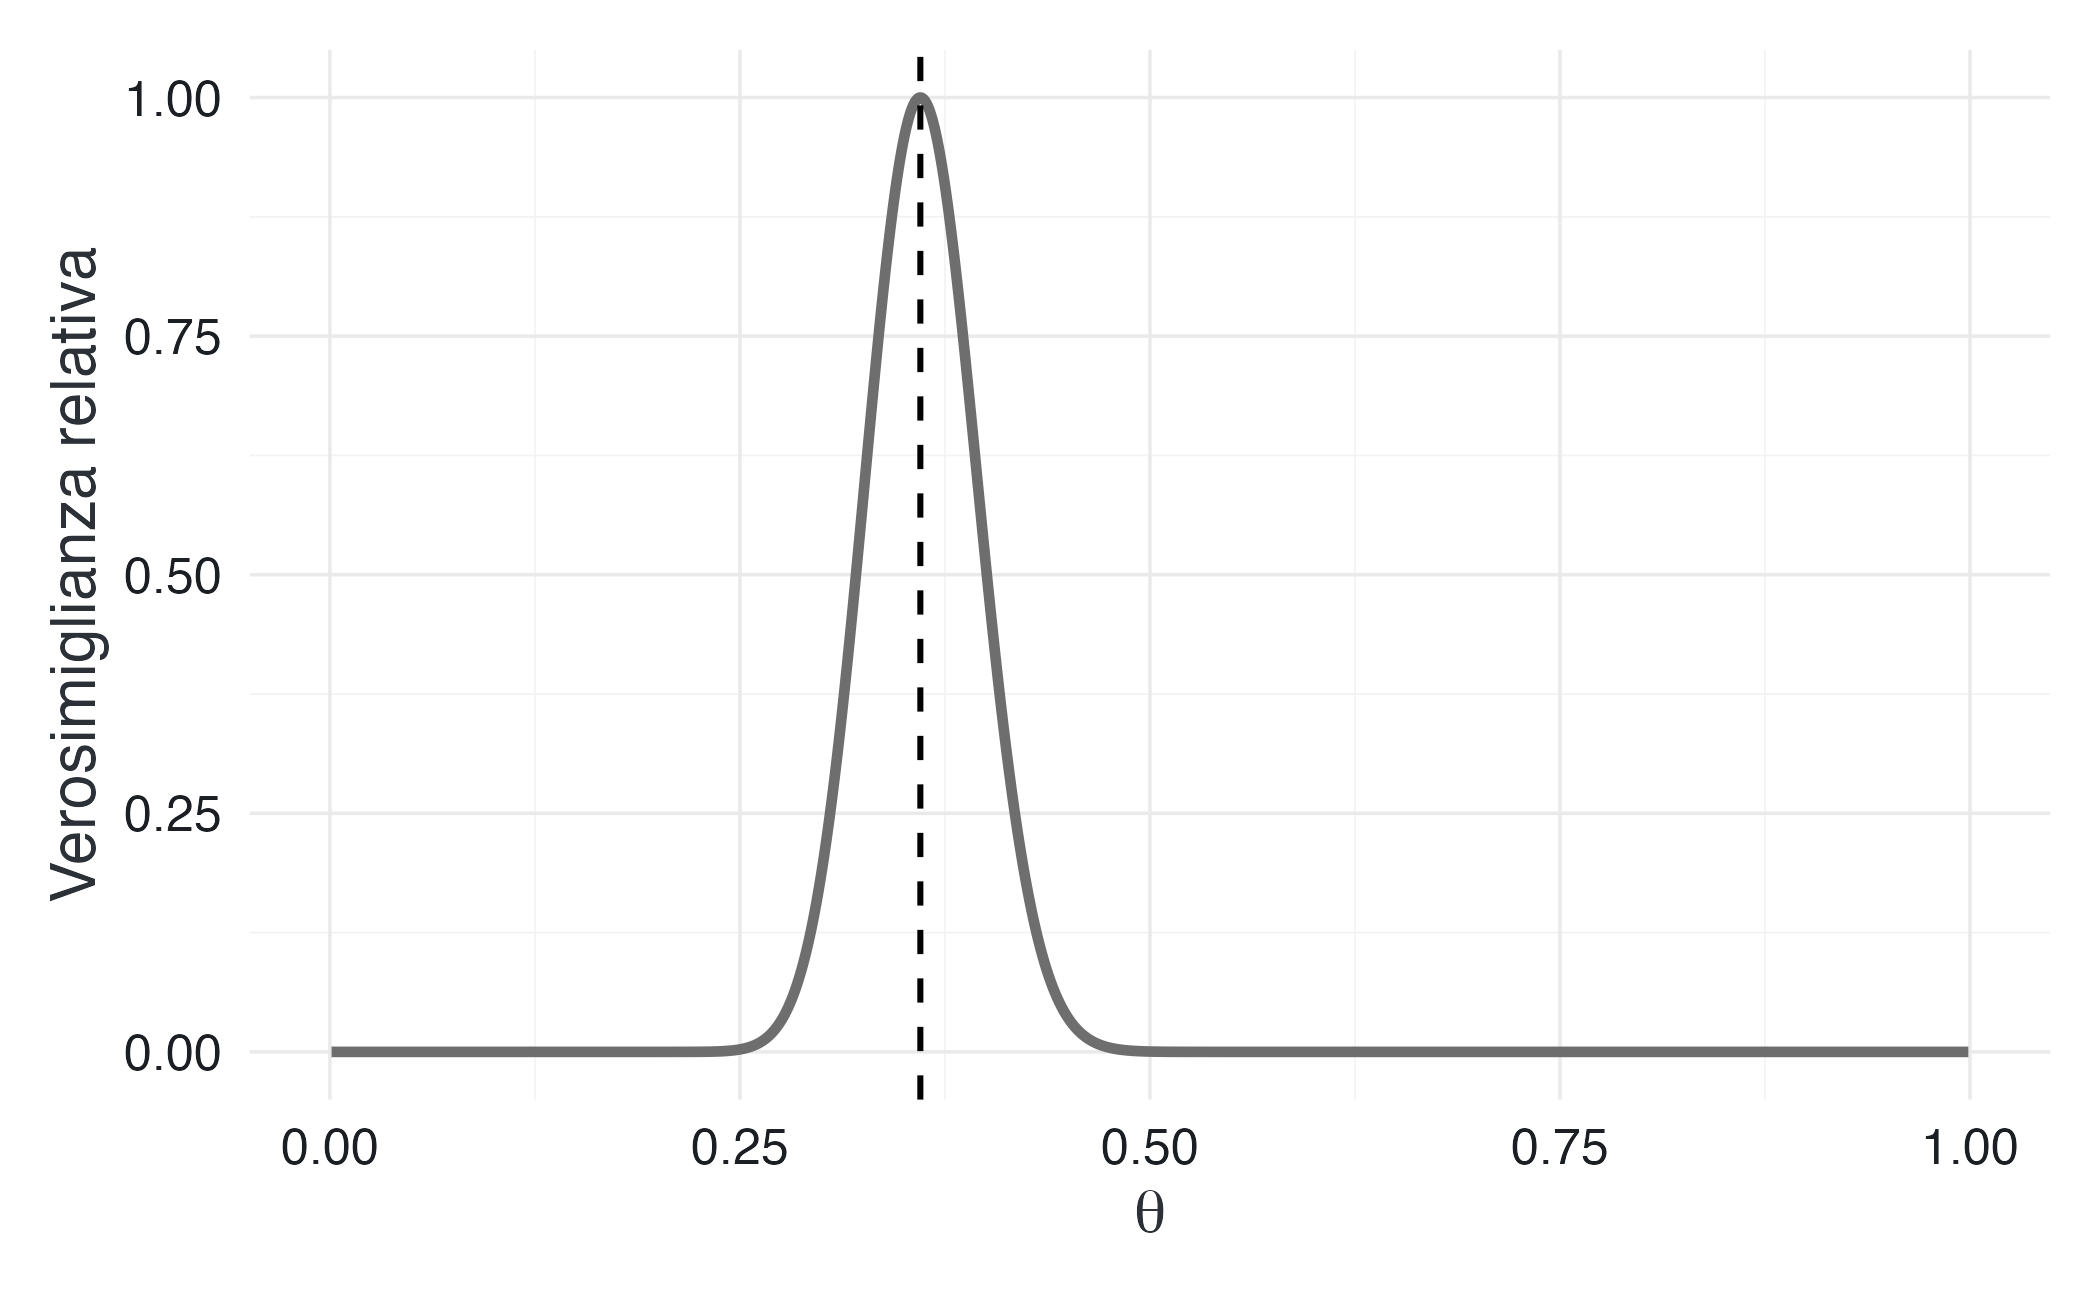
\includegraphics[width=0.85\linewidth,height=\textheight,keepaspectratio]{chapters/probability/14_likelihood_files/figure-pdf/fig-likelihood-remission-1.png}

}

\caption{\label{fig-likelihood-remission}Verosimiglianza relativa per 72
remissioni su 200 pazienti. Il massimo coincide con la proporzione
osservata.}

\end{figure}%

La curva è centrata sul valore osservato, ma la sua larghezza comunica
quanto il campione sia informativo. Una curva larga indica che molti
valori di \(\theta\) restano compatibili con i dati; una curva stretta
indica che i dati discriminano più nettamente tra valori alternativi.

\subsection{Stessa proporzione, diversa quantità di
informazione}\label{stessa-proporzione-diversa-quantituxe0-di-informazione}

Per collegare la verosimiglianza al capitolo precedente, confrontiamo
due studi con la stessa proporzione osservata, ma con dimensioni
campionarie diverse:

\begin{itemize}
\tightlist
\item
  studio piccolo: 9 remissioni su 25 pazienti, \(\hat{\theta}=0.36\);
\item
  studio grande: 72 remissioni su 200 pazienti, \(\hat{\theta}=0.36\).
\end{itemize}

La proporzione osservata è identica, ma la quantità di informazione non
lo è.

\begin{Shaded}
\begin{Highlighting}[]
\NormalTok{theta\_grid }\OtherTok{\textless{}{-}} \FunctionTok{seq}\NormalTok{(}\FloatTok{0.001}\NormalTok{, }\FloatTok{0.999}\NormalTok{, }\AttributeTok{length.out =} \DecValTok{1000}\NormalTok{)}

\NormalTok{lik\_small\_log }\OtherTok{\textless{}{-}} \FunctionTok{dbinom}\NormalTok{(}\DecValTok{9}\NormalTok{, }\AttributeTok{size =} \DecValTok{25}\NormalTok{, }\AttributeTok{prob =}\NormalTok{ theta\_grid, }\AttributeTok{log =} \ConstantTok{TRUE}\NormalTok{)}
\NormalTok{lik\_large\_log }\OtherTok{\textless{}{-}} \FunctionTok{dbinom}\NormalTok{(}\DecValTok{72}\NormalTok{, }\AttributeTok{size =} \DecValTok{200}\NormalTok{, }\AttributeTok{prob =}\NormalTok{ theta\_grid, }\AttributeTok{log =} \ConstantTok{TRUE}\NormalTok{)}

\NormalTok{df\_compare }\OtherTok{\textless{}{-}} \FunctionTok{rbind}\NormalTok{(}
  \FunctionTok{data.frame}\NormalTok{(}
    \AttributeTok{theta =}\NormalTok{ theta\_grid,}
    \AttributeTok{relative\_likelihood =} \FunctionTok{exp}\NormalTok{(lik\_small\_log }\SpecialCharTok{{-}} \FunctionTok{max}\NormalTok{(lik\_small\_log)),}
    \AttributeTok{studio =} \StringTok{"9/25"}
\NormalTok{  ),}
  \FunctionTok{data.frame}\NormalTok{(}
    \AttributeTok{theta =}\NormalTok{ theta\_grid,}
    \AttributeTok{relative\_likelihood =} \FunctionTok{exp}\NormalTok{(lik\_large\_log }\SpecialCharTok{{-}} \FunctionTok{max}\NormalTok{(lik\_large\_log)),}
    \AttributeTok{studio =} \StringTok{"72/200"}
\NormalTok{  )}
\NormalTok{)}

\FunctionTok{ggplot}\NormalTok{(df\_compare, }\FunctionTok{aes}\NormalTok{(}\AttributeTok{x =}\NormalTok{ theta, }\AttributeTok{y =}\NormalTok{ relative\_likelihood, }\AttributeTok{linetype =}\NormalTok{ studio)) }\SpecialCharTok{+}
  \FunctionTok{geom\_line}\NormalTok{(}\AttributeTok{linewidth =} \FloatTok{1.2}\NormalTok{) }\SpecialCharTok{+}
  \FunctionTok{geom\_vline}\NormalTok{(}\AttributeTok{xintercept =} \FloatTok{0.36}\NormalTok{, }\AttributeTok{linetype =} \StringTok{"dashed"}\NormalTok{) }\SpecialCharTok{+}
  \FunctionTok{labs}\NormalTok{(}
    \AttributeTok{x =} \FunctionTok{expression}\NormalTok{(theta),}
    \AttributeTok{y =} \StringTok{"Verosimiglianza relativa"}\NormalTok{,}
    \AttributeTok{linetype =} \StringTok{"Dati osservati"}
\NormalTok{  )}
\end{Highlighting}
\end{Shaded}

\begin{figure}[H]

\centering{

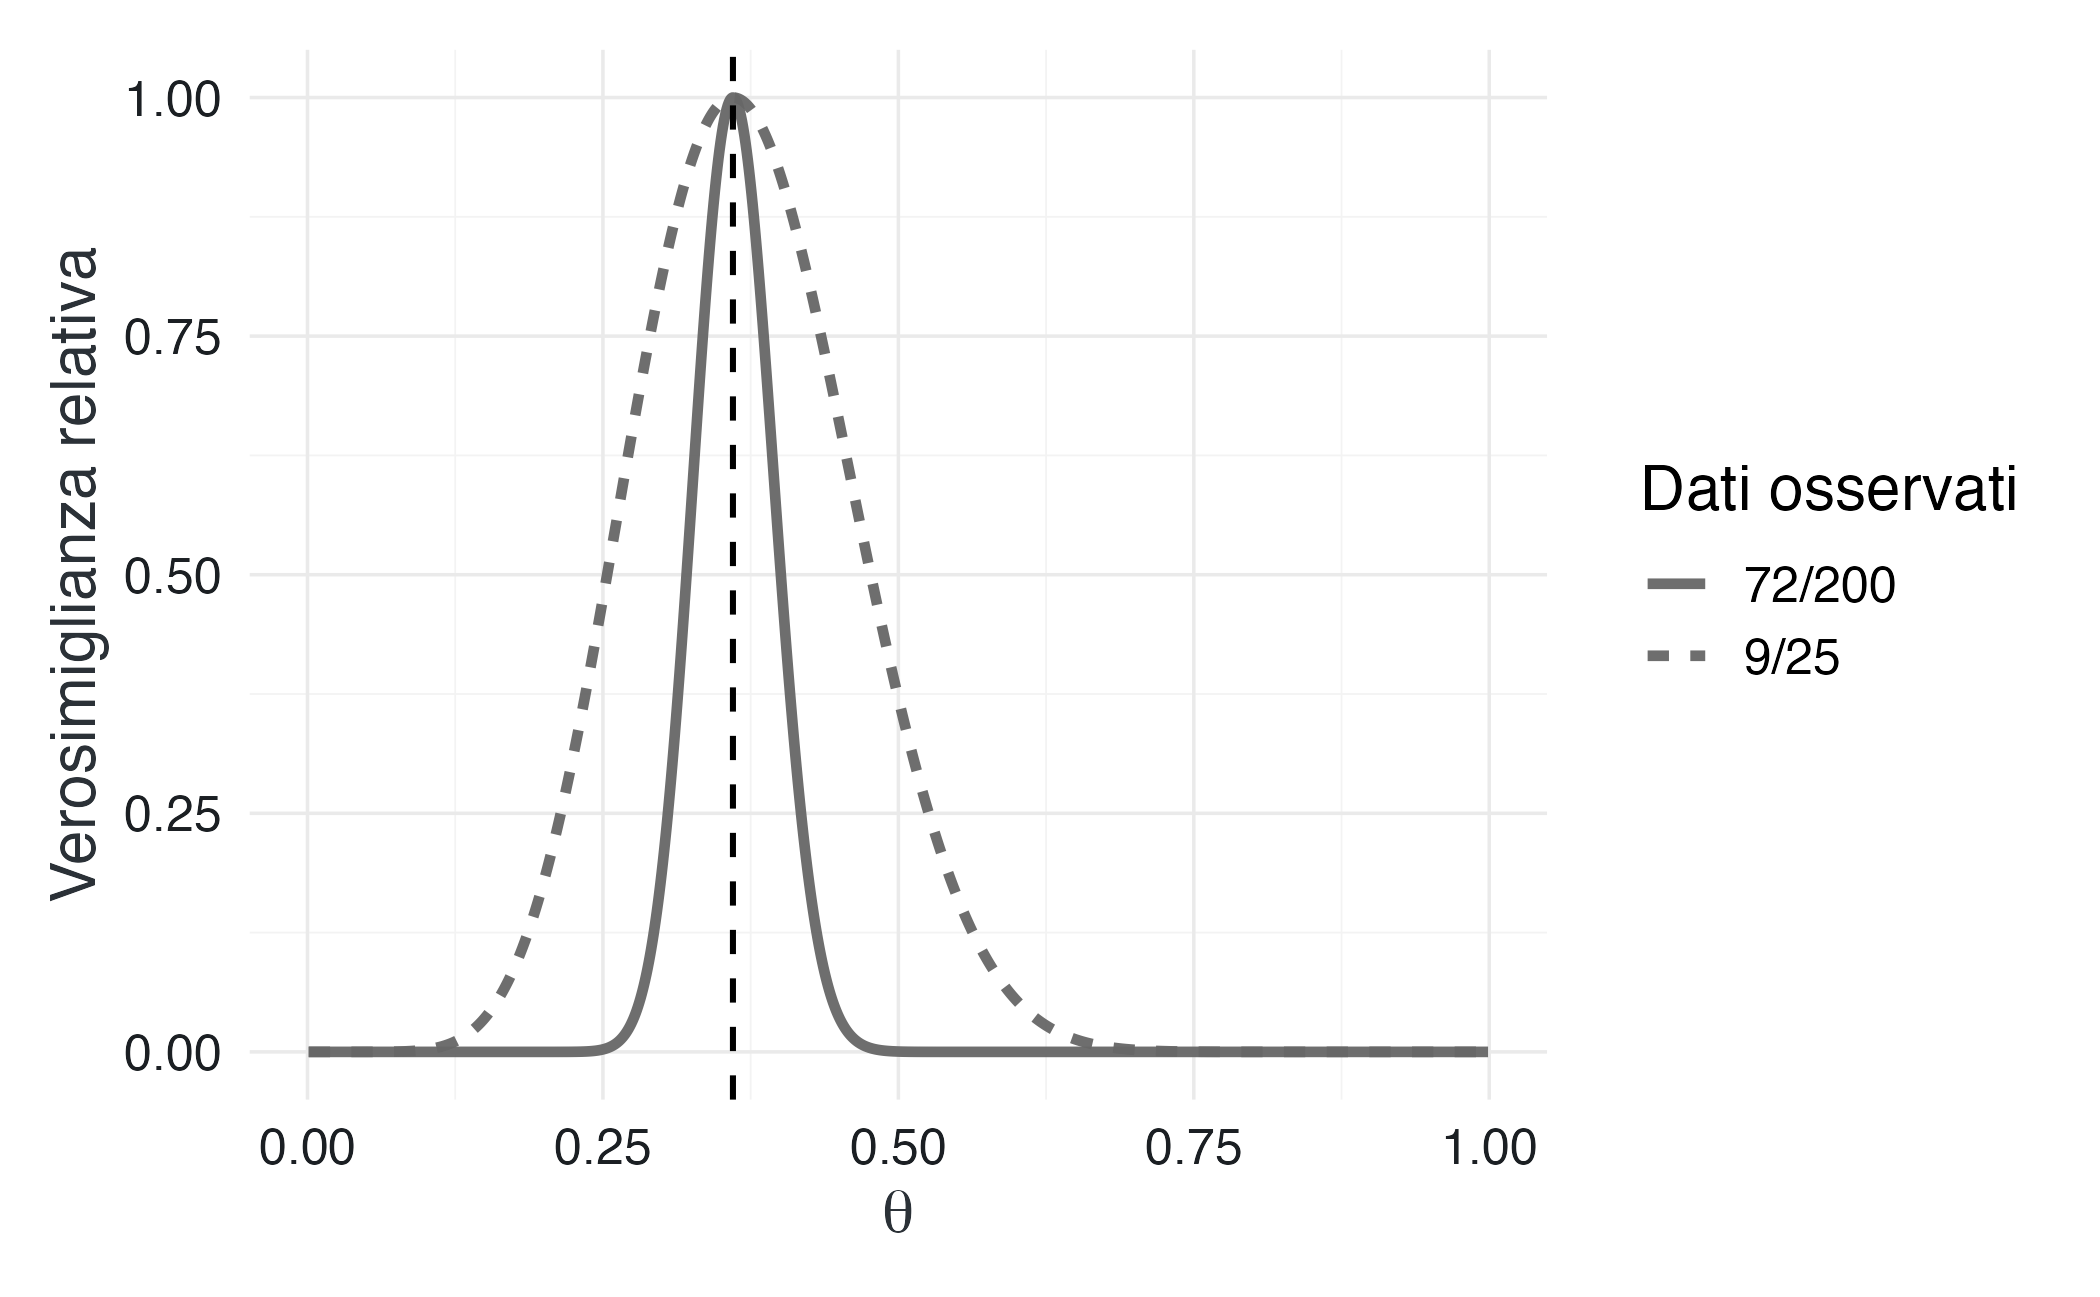
\includegraphics[width=0.85\linewidth,height=\textheight,keepaspectratio]{chapters/probability/14_likelihood_files/figure-pdf/fig-likelihood-same-proportion-1.png}

}

\caption{\label{fig-likelihood-same-proportion}Due studi con la stessa
proporzione osservata ma diversa dimensione campionaria. Il campione più
grande produce una verosimiglianza più concentrata.}

\end{figure}%

Il massimo è lo stesso, perché la proporzione osservata è la stessa.
Tuttavia, la curva basata su 200 pazienti è molto più stretta: i dati
sono più informativi. Questo è il corrispettivo, sulla scala della
verosimiglianza, dell'idea di precisione discussa nel capitolo
precedente.

\begin{tcolorbox}[enhanced jigsaw, arc=.35mm, bottomrule=.15mm, bottomtitle=1mm, breakable, colback=white, colbacktitle=quarto-callout-important-color!10!white, colframe=quarto-callout-important-color-frame, coltitle=black, left=2mm, leftrule=.75mm, opacityback=0, opacitybacktitle=0.6, rightrule=.15mm, title=\textcolor{quarto-callout-important-color}{\faExclamation}\hspace{0.5em}{Collegamento con l'errore standard}, titlerule=0mm, toprule=.15mm, toptitle=1mm]

Nel capitolo precedente abbiamo visto che l'errore standard della
proporzione decresce come \(1/\sqrt{n}\). Qui vediamo la stessa idea da
un'altra prospettiva: al crescere di \(n\), la verosimiglianza tende a
concentrarsi attorno ai valori del parametro più compatibili con i dati.

\end{tcolorbox}

\section{Log-verosimiglianza}\label{sec-log-likelihood}

\subsection{Perché usare il
logaritmo}\label{perchuxe9-usare-il-logaritmo}

Con molti dati, la verosimiglianza è spesso il prodotto di molte
probabilità o densità. Poiché molte di queste quantità sono minori di 1,
il prodotto può diventare estremamente piccolo. Dal punto di vista
computazionale, questo può causare \emph{underflow numerico}: il
computer rappresenta il prodotto come zero anche quando matematicamente
non lo è.

Per evitare questo problema si lavora con la
\textbf{log-verosimiglianza}:

\[
\ell(\theta; y) = \log L(\theta; y).
\]

Nel caso di osservazioni indipendenti:

\[
L(\theta; y_1, \ldots, y_n) = \prod_{i=1}^{n} f(y_i \mid \theta),
\]

quindi:

\[
\ell(\theta; y_1, \ldots, y_n)
= \sum_{i=1}^{n} \log f(y_i \mid \theta).
\]

Il logaritmo trasforma prodotti in somme, che sono più stabili
numericamente e più semplici da analizzare.

\subsection{Massimi equivalenti}\label{massimi-equivalenti}

Il logaritmo naturale è una funzione monotona crescente. Di conseguenza,
il valore di \(\theta\) che massimizza \(L(\theta)\) massimizza anche
\(\ell(\theta)\):

\[
\arg\max_\theta L(\theta) = \arg\max_\theta \ell(\theta).
\]

Quindi lavorare con la log-verosimiglianza non cambia il contenuto
inferenziale della funzione: cambia solo la scala su cui la
rappresentiamo.

\begin{tcolorbox}[enhanced jigsaw, arc=.35mm, bottomrule=.15mm, bottomtitle=1mm, breakable, colback=white, colbacktitle=quarto-callout-caution-color!10!white, colframe=quarto-callout-caution-color-frame, coltitle=black, left=2mm, leftrule=.75mm, opacityback=0, opacitybacktitle=0.6, rightrule=.15mm, title=\textcolor{quarto-callout-caution-color}{\faFire}\hspace{0.5em}{Esempio pratico: underflow e log-verosimiglianza}, titlerule=0mm, toprule=.15mm, toptitle=1mm]

\begin{Shaded}
\begin{Highlighting}[]
\FunctionTok{set.seed}\NormalTok{(}\DecValTok{42}\NormalTok{)}
\NormalTok{n }\OtherTok{\textless{}{-}} \DecValTok{2000}
\NormalTok{theta }\OtherTok{\textless{}{-}} \FloatTok{0.35}
\NormalTok{dati }\OtherTok{\textless{}{-}} \FunctionTok{rbinom}\NormalTok{(n, }\AttributeTok{size =} \DecValTok{1}\NormalTok{, }\AttributeTok{prob =}\NormalTok{ theta)}

\CommentTok{\# Prodotto diretto delle probabilità: può collassare numericamente a zero}
\NormalTok{lik\_diretta }\OtherTok{\textless{}{-}} \FunctionTok{prod}\NormalTok{(}\FunctionTok{dbinom}\NormalTok{(dati, }\AttributeTok{size =} \DecValTok{1}\NormalTok{, }\AttributeTok{prob =}\NormalTok{ theta))}

\CommentTok{\# Somma dei log: stabile}
\NormalTok{log\_lik }\OtherTok{\textless{}{-}} \FunctionTok{sum}\NormalTok{(}\FunctionTok{dbinom}\NormalTok{(dati, }\AttributeTok{size =} \DecValTok{1}\NormalTok{, }\AttributeTok{prob =}\NormalTok{ theta, }\AttributeTok{log =} \ConstantTok{TRUE}\NormalTok{))}

\FunctionTok{cat}\NormalTok{(}\StringTok{"Verosimiglianza diretta:"}\NormalTok{, lik\_diretta, }\StringTok{"}\SpecialCharTok{\textbackslash{}n}\StringTok{"}\NormalTok{)}
\CommentTok{\#\textgreater{} Verosimiglianza diretta: 0}
\FunctionTok{cat}\NormalTok{(}\StringTok{"Log{-}verosimiglianza:"}\NormalTok{, log\_lik, }\StringTok{"}\SpecialCharTok{\textbackslash{}n}\StringTok{"}\NormalTok{)}
\CommentTok{\#\textgreater{} Log{-}verosimiglianza: {-}1294}
\end{Highlighting}
\end{Shaded}

\end{tcolorbox}

\subsection{Log-verosimiglianza
binomiale}\label{log-verosimiglianza-binomiale}

Per il modello binomiale:

\[
L(\theta; y,n) \propto \theta^y(1-\theta)^{n-y}.
\]

La log-verosimiglianza, trascurando la costante che non dipende da
\(\theta\), è:

\[
\ell(\theta; y,n)
= y\log\theta + (n-y)\log(1-\theta).
\]

Questa forma rende evidente come il dato osservato contribuisca
all'evidenza:

\begin{itemize}
\tightlist
\item
  i successi aumentano il supporto per valori alti di \(\theta\);
\item
  gli insuccessi aumentano il supporto per valori bassi di \(\theta\);
\item
  il bilanciamento tra successi e insuccessi determina il punto di
  massimo;
\item
  la dimensione del campione determina quanto la curva sia concentrata.
\end{itemize}

\section{Verosimiglianza congiunta e accumulo
dell'evidenza}\label{sec-joint-likelihood}

\subsection{Osservazioni indipendenti}\label{osservazioni-indipendenti}

Se i dati sono indipendenti condizionatamente a \(\theta\), la
verosimiglianza congiunta è il prodotto delle verosimiglianze
individuali:

\[
L(\theta; y_1, \ldots, y_n)
= \prod_{i=1}^{n} f(y_i \mid \theta).
\]

Sulla scala logaritmica:

\[
\ell(\theta; y_1, \ldots, y_n)
= \sum_{i=1}^{n}\log f(y_i \mid \theta).
\]

Questa formula esprime in modo molto semplice l'accumulo dell'evidenza:
ogni osservazione aggiunge un contributo alla log-verosimiglianza
complessiva.

\subsection{Combinare studi
indipendenti}\label{combinare-studi-indipendenti}

La stessa idea vale quando combiniamo studi indipendenti. Supponiamo che
quattro studi misurino lo stesso parametro \(\theta\), per esempio la
probabilità di successo di un intervento:

{\def\LTcaptype{none} % do not increment counter
\begin{longtable}[]{@{}rrr@{}}
\toprule\noalign{}
Studio & Successi & Totale \\
\midrule\noalign{}
\endhead
\bottomrule\noalign{}
\endlastfoot
1 & 23 & 30 \\
2 & 20 & 28 \\
3 & 29 & 40 \\
4 & 29 & 36 \\
\end{longtable}
}

Se assumiamo che tutti gli studi condividano lo stesso valore di
\(\theta\) e siano indipendenti, la log-verosimiglianza complessiva è:

\[
\ell(\theta)
= \sum_{j=1}^{4}\left[y_j\log\theta + (n_j-y_j)\log(1-\theta)\right].
\]

\begin{Shaded}
\begin{Highlighting}[]
\NormalTok{studi }\OtherTok{\textless{}{-}} \FunctionTok{data.frame}\NormalTok{(}
  \AttributeTok{successi =} \FunctionTok{c}\NormalTok{(}\DecValTok{23}\NormalTok{, }\DecValTok{20}\NormalTok{, }\DecValTok{29}\NormalTok{, }\DecValTok{29}\NormalTok{),}
  \AttributeTok{prove    =} \FunctionTok{c}\NormalTok{(}\DecValTok{30}\NormalTok{, }\DecValTok{28}\NormalTok{, }\DecValTok{40}\NormalTok{, }\DecValTok{36}\NormalTok{)}
\NormalTok{)}

\NormalTok{log\_lik\_congiunta }\OtherTok{\textless{}{-}} \ControlFlowTok{function}\NormalTok{(theta) \{}
  \FunctionTok{sum}\NormalTok{(studi}\SpecialCharTok{$}\NormalTok{successi }\SpecialCharTok{*} \FunctionTok{log}\NormalTok{(theta) }\SpecialCharTok{+}
\NormalTok{        (studi}\SpecialCharTok{$}\NormalTok{prove }\SpecialCharTok{{-}}\NormalTok{ studi}\SpecialCharTok{$}\NormalTok{successi) }\SpecialCharTok{*} \FunctionTok{log}\NormalTok{(}\DecValTok{1} \SpecialCharTok{{-}}\NormalTok{ theta))}
\NormalTok{\}}

\NormalTok{theta\_seq }\OtherTok{\textless{}{-}} \FunctionTok{seq}\NormalTok{(}\FloatTok{0.5}\NormalTok{, }\FloatTok{0.9}\NormalTok{, }\AttributeTok{length.out =} \DecValTok{400}\NormalTok{)}
\NormalTok{log\_lik\_vals }\OtherTok{\textless{}{-}} \FunctionTok{sapply}\NormalTok{(theta\_seq, log\_lik\_congiunta)}
\NormalTok{rel\_lik\_vals }\OtherTok{\textless{}{-}} \FunctionTok{exp}\NormalTok{(log\_lik\_vals }\SpecialCharTok{{-}} \FunctionTok{max}\NormalTok{(log\_lik\_vals))}

\FunctionTok{ggplot}\NormalTok{(}\FunctionTok{data.frame}\NormalTok{(}\AttributeTok{theta =}\NormalTok{ theta\_seq, }\AttributeTok{rel\_lik =}\NormalTok{ rel\_lik\_vals),}
       \FunctionTok{aes}\NormalTok{(}\AttributeTok{x =}\NormalTok{ theta, }\AttributeTok{y =}\NormalTok{ rel\_lik)) }\SpecialCharTok{+}
  \FunctionTok{geom\_line}\NormalTok{(}\AttributeTok{linewidth =} \FloatTok{1.2}\NormalTok{) }\SpecialCharTok{+}
  \FunctionTok{geom\_vline}\NormalTok{(}\AttributeTok{xintercept =} \FunctionTok{sum}\NormalTok{(studi}\SpecialCharTok{$}\NormalTok{successi) }\SpecialCharTok{/} \FunctionTok{sum}\NormalTok{(studi}\SpecialCharTok{$}\NormalTok{prove),}
             \AttributeTok{linetype =} \StringTok{"dashed"}\NormalTok{) }\SpecialCharTok{+}
  \FunctionTok{labs}\NormalTok{(}
    \AttributeTok{x =} \FunctionTok{expression}\NormalTok{(theta),}
    \AttributeTok{y =} \StringTok{"Verosimiglianza relativa"}
\NormalTok{  )}
\end{Highlighting}
\end{Shaded}

\begin{figure}[H]

\centering{

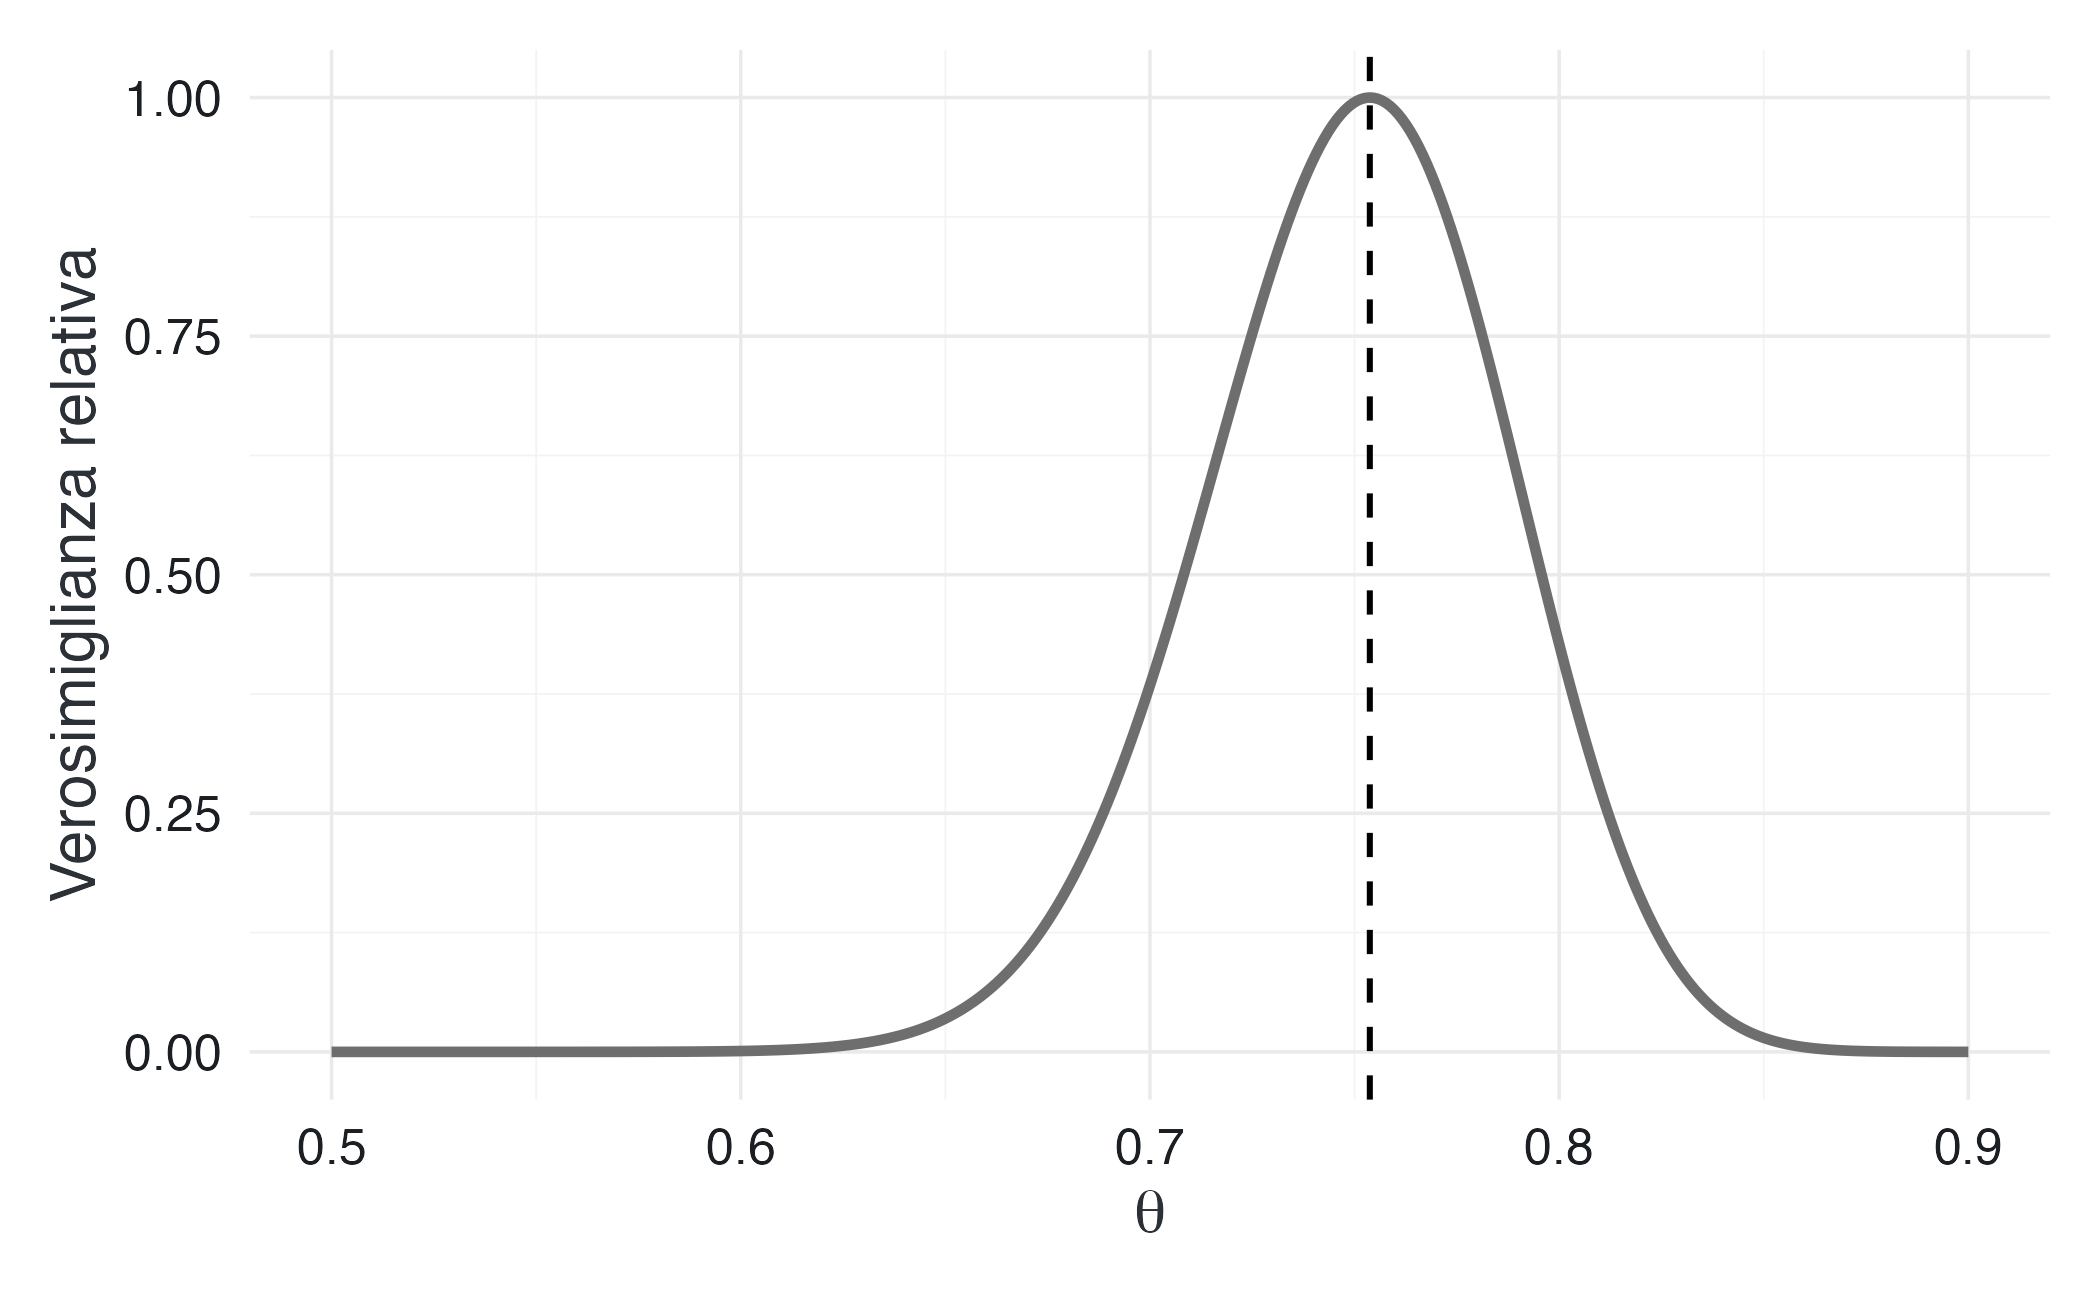
\includegraphics[width=0.85\linewidth,height=\textheight,keepaspectratio]{chapters/probability/14_likelihood_files/figure-pdf/fig-joint-likelihood-studies-1.png}

}

\caption{\label{fig-joint-likelihood-studies}Log-verosimiglianza
congiunta ottenuta combinando quattro studi indipendenti.}

\end{figure}%

La curva risultante riassume l'evidenza complessiva. Non abbiamo fatto
una media semplice delle proporzioni: abbiamo combinato le
verosimiglianze, cioè l'informazione che ciascuno studio fornisce su
\(\theta\).

\begin{tcolorbox}[enhanced jigsaw, arc=.35mm, bottomrule=.15mm, bottomtitle=1mm, breakable, colback=white, colbacktitle=quarto-callout-note-color!10!white, colframe=quarto-callout-note-color-frame, coltitle=black, left=2mm, leftrule=.75mm, opacityback=0, opacitybacktitle=0.6, rightrule=.15mm, title=\textcolor{quarto-callout-note-color}{\faInfo}\hspace{0.5em}{Connessione con la meta-analisi}, titlerule=0mm, toprule=.15mm, toptitle=1mm]

Nel capitolo precedente abbiamo introdotto l'idea che evidenze
indipendenti si combinano sommando le precisioni. La verosimiglianza
fornisce la formulazione generale di questa idea: nel caso indipendente,
le verosimiglianze si moltiplicano e le log-verosimiglianze si sommano.

\end{tcolorbox}

\section{Verosimiglianza gaussiana}\label{sec-normal-likelihood}

La distribuzione Normale è particolarmente importante perché permette di
collegare in modo chiaro verosimiglianza, media campionaria, errore
standard e precisione.

Supponiamo di osservare misure continue, per esempio punteggi a una
scala psicologica, tempi di reazione o indici psicofisiologici.
Assumiamo che:

\[
Y_i \mid \mu \sim \mathcal{N}(\mu, \sigma^2),
\]

dove la media \(\mu\) è ignota e la deviazione standard \(\sigma\) è
nota.

\subsection{Una singola osservazione}\label{una-singola-osservazione}

Se osserviamo un solo valore \(y\), la verosimiglianza per \(\mu\) è:

\[
L(\mu; y)
= \frac{1}{\sigma\sqrt{2\pi}}
\exp\left[-\frac{(y-\mu)^2}{2\sigma^2}\right].
\]

Come funzione di \(\mu\), questa curva è centrata sul dato osservato
\(y\). I valori di \(\mu\) vicini a \(y\) rendono il dato più
plausibile; quelli lontani lo rendono meno plausibile.

\begin{Shaded}
\begin{Highlighting}[]
\NormalTok{y\_obs }\OtherTok{\textless{}{-}} \DecValTok{114}
\NormalTok{sigma }\OtherTok{\textless{}{-}} \DecValTok{15}
\NormalTok{mu\_grid }\OtherTok{\textless{}{-}} \FunctionTok{seq}\NormalTok{(}\DecValTok{70}\NormalTok{, }\DecValTok{160}\NormalTok{, }\AttributeTok{length.out =} \DecValTok{500}\NormalTok{)}
\NormalTok{log\_lik }\OtherTok{\textless{}{-}} \FunctionTok{dnorm}\NormalTok{(y\_obs, }\AttributeTok{mean =}\NormalTok{ mu\_grid, }\AttributeTok{sd =}\NormalTok{ sigma, }\AttributeTok{log =} \ConstantTok{TRUE}\NormalTok{)}
\NormalTok{rel\_lik }\OtherTok{\textless{}{-}} \FunctionTok{exp}\NormalTok{(log\_lik }\SpecialCharTok{{-}} \FunctionTok{max}\NormalTok{(log\_lik))}

\FunctionTok{ggplot}\NormalTok{(}\FunctionTok{data.frame}\NormalTok{(}\AttributeTok{mu =}\NormalTok{ mu\_grid, }\AttributeTok{rel\_lik =}\NormalTok{ rel\_lik),}
       \FunctionTok{aes}\NormalTok{(}\AttributeTok{x =}\NormalTok{ mu, }\AttributeTok{y =}\NormalTok{ rel\_lik)) }\SpecialCharTok{+}
  \FunctionTok{geom\_line}\NormalTok{(}\AttributeTok{linewidth =} \FloatTok{1.2}\NormalTok{) }\SpecialCharTok{+}
  \FunctionTok{geom\_vline}\NormalTok{(}\AttributeTok{xintercept =}\NormalTok{ y\_obs, }\AttributeTok{linetype =} \StringTok{"dashed"}\NormalTok{) }\SpecialCharTok{+}
  \FunctionTok{labs}\NormalTok{(}
    \AttributeTok{x =} \FunctionTok{expression}\NormalTok{(mu),}
    \AttributeTok{y =} \StringTok{"Verosimiglianza relativa"}
\NormalTok{  )}
\end{Highlighting}
\end{Shaded}

\begin{figure}[H]

\centering{

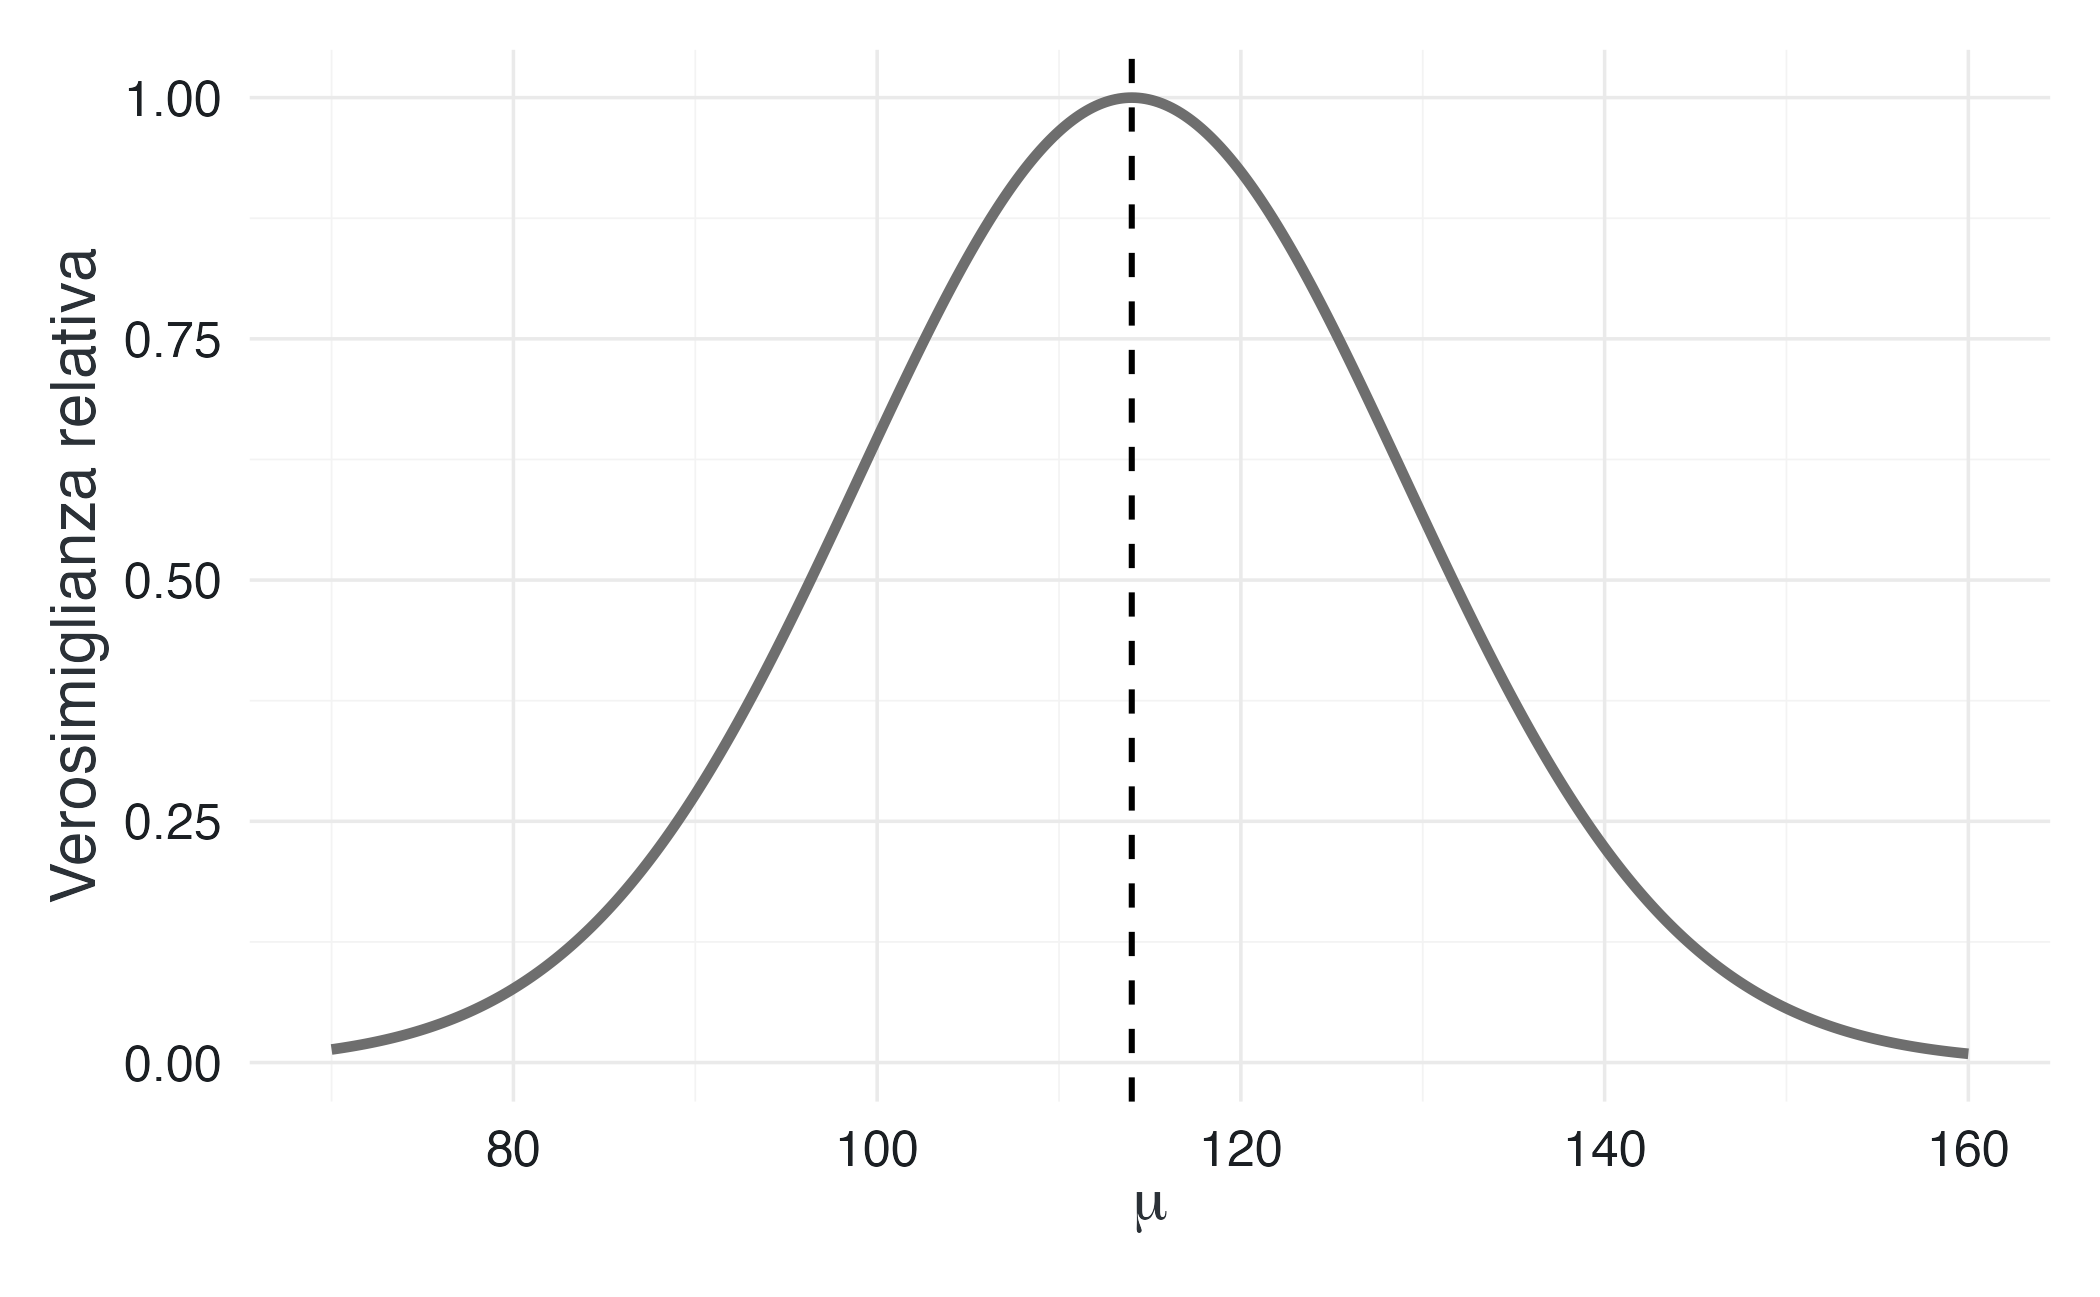
\includegraphics[width=0.85\linewidth,height=\textheight,keepaspectratio]{chapters/probability/14_likelihood_files/figure-pdf/fig-normal-likelihood-single-1.png}

}

\caption{\label{fig-normal-likelihood-single}Verosimiglianza gaussiana
per una singola osservazione.}

\end{figure}%

Una singola osservazione fornisce informazione, ma la curva è ancora
ampia. Molti valori di \(\mu\) restano compatibili con il dato.

\subsection{Un campione gaussiano}\label{un-campione-gaussiano}

Con un campione indipendente \(y_1,\ldots,y_n\), la verosimiglianza
congiunta è:

\[
L(\mu; y_1,\ldots,y_n)
= \prod_{i=1}^{n}
\frac{1}{\sigma\sqrt{2\pi}}
\exp\left[-\frac{(y_i-\mu)^2}{2\sigma^2}\right].
\]

La log-verosimiglianza è:

\[
\ell(\mu)
= -\frac{n}{2}\log(2\pi\sigma^2)
- \frac{1}{2\sigma^2}\sum_{i=1}^{n}(y_i-\mu)^2.
\]

L'unico termine che dipende da \(\mu\) è la somma dei quadrati degli
scarti. La verosimiglianza è massima quando questa somma è minima, cioè
quando:

\[
\mu = \bar{y}.
\]

Più importante ancora, la forma della verosimiglianza può essere
riscritta come:

\[
L(\mu; y_1,\ldots,y_n)
\propto
\exp\left[-\frac{n}{2\sigma^2}(\mu-\bar{y})^2\right].
\]

Questa è la forma di una curva normale in \(\mu\), centrata su
\(\bar{y}\) e con varianza:

\[
\frac{\sigma^2}{n}.
\]

Dunque, la precisione della verosimiglianza per \(\mu\) è:

\[
\tau_{\text{dati}} = \frac{n}{\sigma^2}.
\]

Questo è lo stesso risultato visto nel capitolo precedente dal punto di
vista dell'errore standard della media campionaria.

\begin{Shaded}
\begin{Highlighting}[]
\NormalTok{y }\OtherTok{\textless{}{-}} \FunctionTok{c}\NormalTok{(}\DecValTok{26}\NormalTok{, }\DecValTok{35}\NormalTok{, }\DecValTok{30}\NormalTok{, }\DecValTok{25}\NormalTok{, }\DecValTok{44}\NormalTok{, }\DecValTok{30}\NormalTok{, }\DecValTok{33}\NormalTok{, }\DecValTok{43}\NormalTok{, }\DecValTok{22}\NormalTok{, }\DecValTok{43}\NormalTok{, }\DecValTok{24}\NormalTok{, }\DecValTok{19}\NormalTok{, }\DecValTok{39}\NormalTok{, }\DecValTok{31}\NormalTok{, }\DecValTok{25}\NormalTok{,}
       \DecValTok{28}\NormalTok{, }\DecValTok{35}\NormalTok{, }\DecValTok{30}\NormalTok{, }\DecValTok{26}\NormalTok{, }\DecValTok{31}\NormalTok{, }\DecValTok{41}\NormalTok{, }\DecValTok{36}\NormalTok{, }\DecValTok{26}\NormalTok{, }\DecValTok{35}\NormalTok{, }\DecValTok{33}\NormalTok{, }\DecValTok{28}\NormalTok{, }\DecValTok{27}\NormalTok{, }\DecValTok{34}\NormalTok{, }\DecValTok{27}\NormalTok{, }\DecValTok{22}\NormalTok{)}
\NormalTok{sigma }\OtherTok{\textless{}{-}} \FloatTok{6.5}
\NormalTok{mu\_grid }\OtherTok{\textless{}{-}} \FunctionTok{seq}\NormalTok{(}\DecValTok{25}\NormalTok{, }\DecValTok{40}\NormalTok{, }\AttributeTok{length.out =} \DecValTok{500}\NormalTok{)}

\NormalTok{log\_lik }\OtherTok{\textless{}{-}} \FunctionTok{sapply}\NormalTok{(mu\_grid, }\ControlFlowTok{function}\NormalTok{(mu) \{}
  \FunctionTok{sum}\NormalTok{(}\FunctionTok{dnorm}\NormalTok{(y, }\AttributeTok{mean =}\NormalTok{ mu, }\AttributeTok{sd =}\NormalTok{ sigma, }\AttributeTok{log =} \ConstantTok{TRUE}\NormalTok{))}
\NormalTok{\})}

\NormalTok{rel\_lik }\OtherTok{\textless{}{-}} \FunctionTok{exp}\NormalTok{(log\_lik }\SpecialCharTok{{-}} \FunctionTok{max}\NormalTok{(log\_lik))}

\FunctionTok{ggplot}\NormalTok{(}\FunctionTok{data.frame}\NormalTok{(}\AttributeTok{mu =}\NormalTok{ mu\_grid, }\AttributeTok{rel\_lik =}\NormalTok{ rel\_lik),}
       \FunctionTok{aes}\NormalTok{(}\AttributeTok{x =}\NormalTok{ mu, }\AttributeTok{y =}\NormalTok{ rel\_lik)) }\SpecialCharTok{+}
  \FunctionTok{geom\_line}\NormalTok{(}\AttributeTok{linewidth =} \FloatTok{1.2}\NormalTok{) }\SpecialCharTok{+}
  \FunctionTok{geom\_vline}\NormalTok{(}\AttributeTok{xintercept =} \FunctionTok{mean}\NormalTok{(y), }\AttributeTok{linetype =} \StringTok{"dashed"}\NormalTok{) }\SpecialCharTok{+}
  \FunctionTok{labs}\NormalTok{(}
    \AttributeTok{x =} \FunctionTok{expression}\NormalTok{(mu),}
    \AttributeTok{y =} \StringTok{"Verosimiglianza relativa"}
\NormalTok{  )}
\end{Highlighting}
\end{Shaded}

\begin{figure}[H]

\centering{

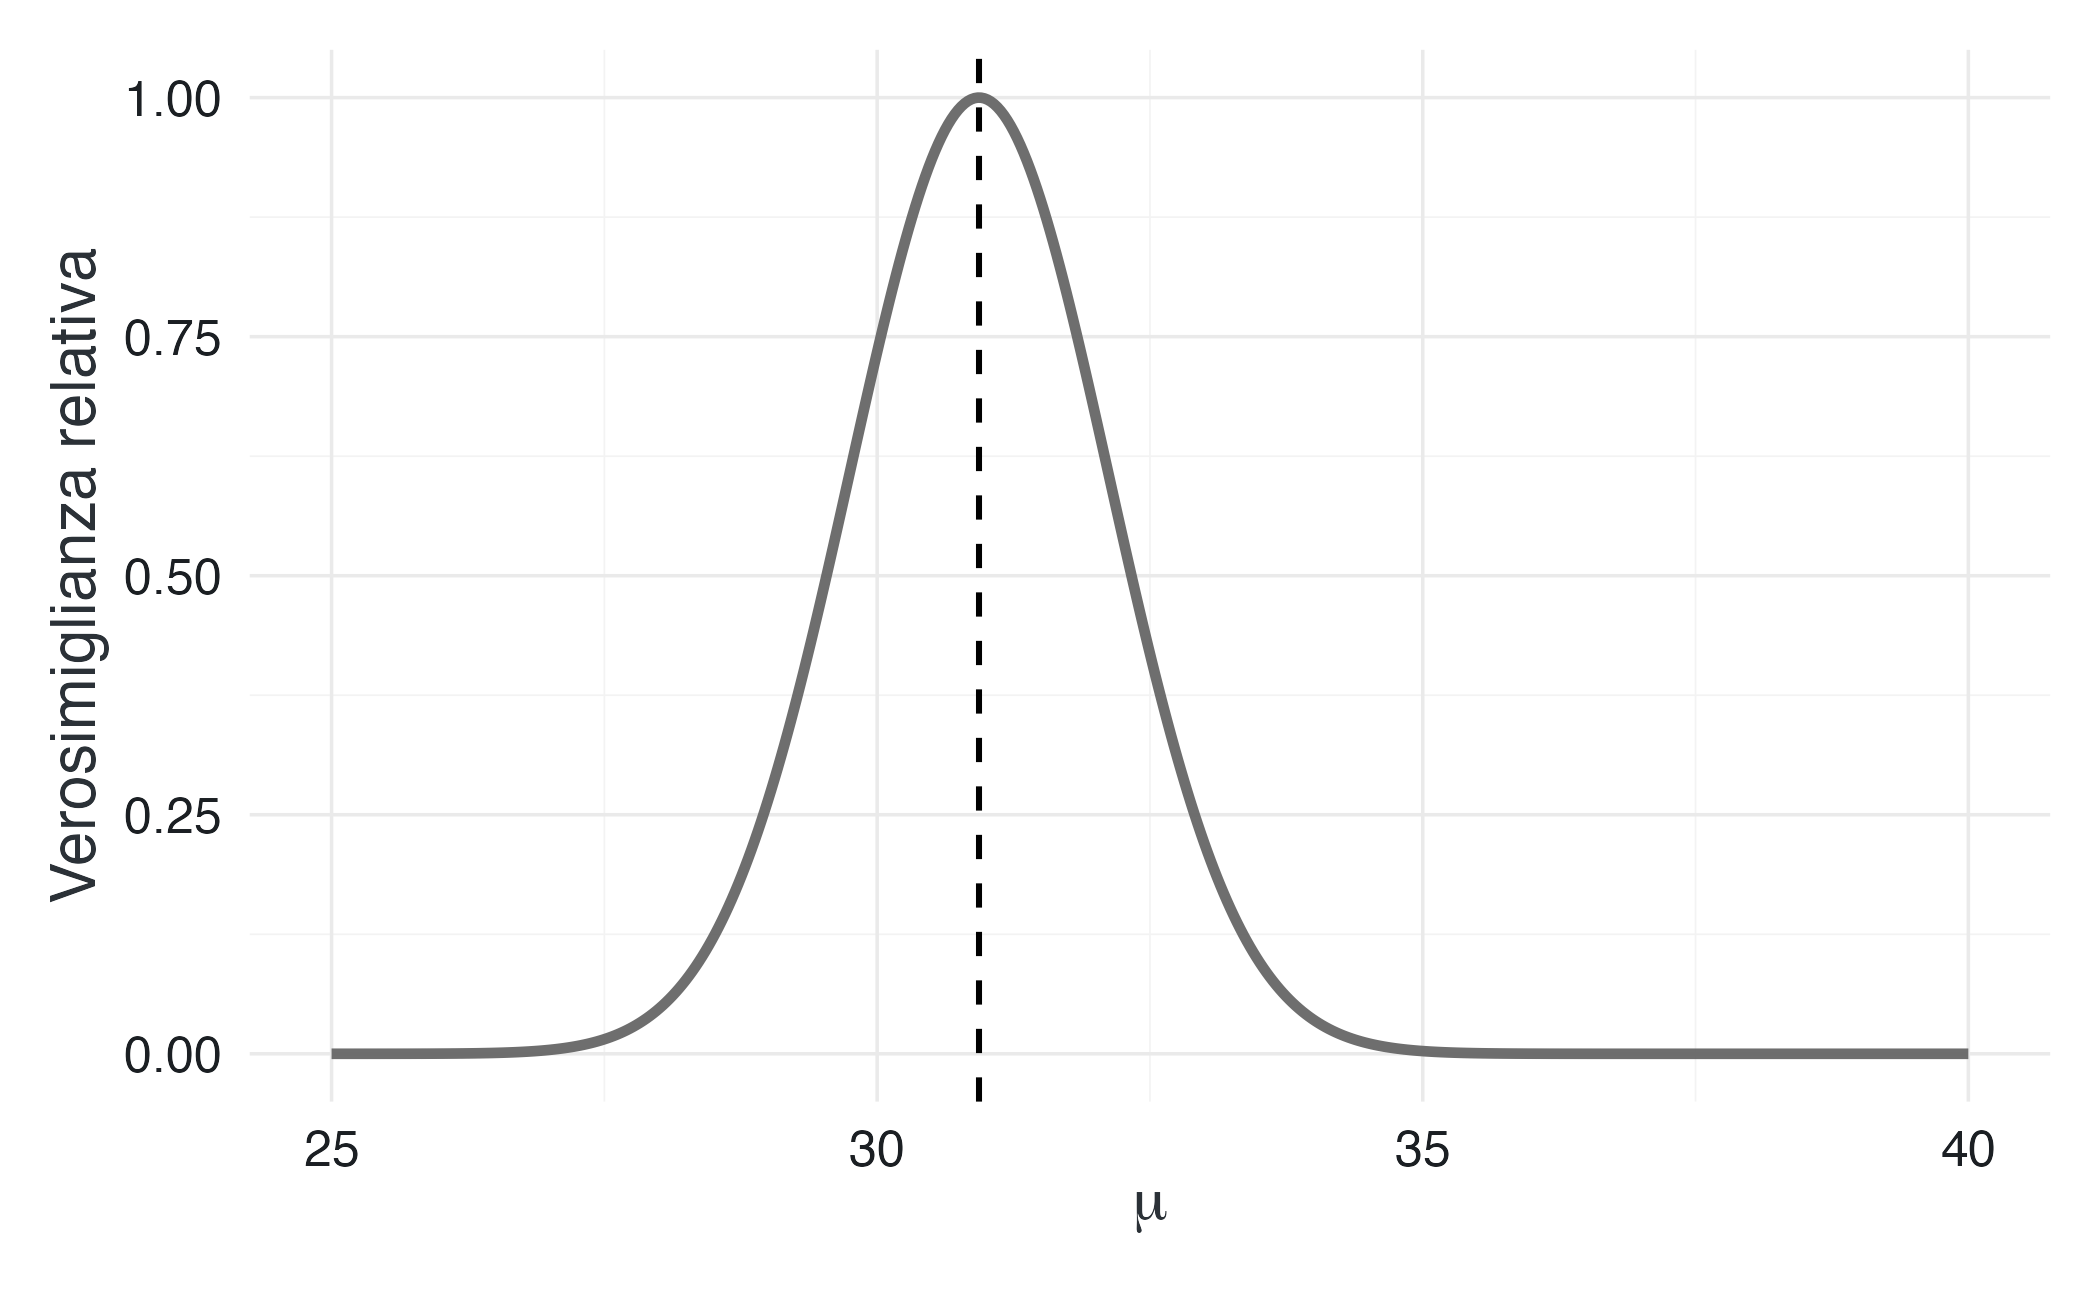
\includegraphics[width=0.85\linewidth,height=\textheight,keepaspectratio]{chapters/probability/14_likelihood_files/figure-pdf/fig-normal-likelihood-sample-1.png}

}

\caption{\label{fig-normal-likelihood-sample}Verosimiglianza gaussiana
relativa per la media di un campione.}

\end{figure}%

\begin{tcolorbox}[enhanced jigsaw, arc=.35mm, bottomrule=.15mm, bottomtitle=1mm, breakable, colback=white, colbacktitle=quarto-callout-important-color!10!white, colframe=quarto-callout-important-color-frame, coltitle=black, left=2mm, leftrule=.75mm, opacityback=0, opacitybacktitle=0.6, rightrule=.15mm, title=\textcolor{quarto-callout-important-color}{\faExclamation}\hspace{0.5em}{Risultato centrale}, titlerule=0mm, toprule=.15mm, toptitle=1mm]

Nel modello gaussiano con varianza nota, la verosimiglianza per la media
ha precisione \(n/\sigma^2\). Questo spiega perché, nell'aggiornamento
bayesiano normale--normale, la posterior può essere vista come una media
pesata tra prior e dati, con pesi proporzionali alle rispettive
precisioni.

\end{tcolorbox}

\section{Il ruolo della massima verosimiglianza}\label{sec-mle-role}

La verosimiglianza può essere usata per ottenere una stima puntuale: il
valore del parametro che massimizza la funzione.

\[
\hat{\theta}_{\text{MLE}}
= \arg\max_{\theta} L(\theta; y).
\]

Questa è la \textbf{stima di massima verosimiglianza} (\emph{maximum
likelihood estimate}, MLE). Nel modello binomiale:

\[
\hat{\theta}_{\text{MLE}} = \frac{y}{n}.
\]

Nel modello gaussiano con varianza nota:

\[
\hat{\mu}_{\text{MLE}} = \bar{y}.
\]

\subsection{Perché parlarne in un manuale
bayesiano?}\label{perchuxe9-parlarne-in-un-manuale-bayesiano}

La MLE è un concetto frequentista, ma è utile anche qui per tre ragioni:

\begin{enumerate}
\def\labelenumi{\arabic{enumi}.}
\tightlist
\item
  identifica il punto in cui la verosimiglianza raggiunge il massimo;
\item
  aiuta a leggere graficamente le curve di verosimiglianza;
\item
  fornisce un confronto con la moda della posterior bayesiana.
\end{enumerate}

Tuttavia, la MLE non è l'obiettivo dell'inferenza bayesiana. Dal punto
di vista bayesiano, l'intera forma della verosimiglianza è più
importante del solo punto di massimo.

\begin{tcolorbox}[enhanced jigsaw, arc=.35mm, bottomrule=.15mm, bottomtitle=1mm, breakable, colback=white, colbacktitle=quarto-callout-note-color!10!white, colframe=quarto-callout-note-color-frame, coltitle=black, left=2mm, leftrule=.75mm, opacityback=0, opacitybacktitle=0.6, rightrule=.15mm, title=\textcolor{quarto-callout-note-color}{\faInfo}\hspace{0.5em}{MLE, MAP e posterior}, titlerule=0mm, toprule=.15mm, toptitle=1mm]

Se la prior è uniforme sullo spazio dei parametri, la moda della
distribuzione a posteriori coincide spesso con la MLE. Con prior
informative, invece, la moda a posteriori (\emph{maximum a posteriori},
MAP) può essere diversa dalla MLE, perché incorpora anche le credenze a
priori.

\end{tcolorbox}

\begin{tcolorbox}[enhanced jigsaw, arc=.35mm, bottomrule=.15mm, bottomtitle=1mm, breakable, colback=white, colbacktitle=quarto-callout-note-color!10!white, colframe=quarto-callout-note-color-frame, coltitle=black, left=2mm, leftrule=.75mm, opacityback=0, opacitybacktitle=0.6, rightrule=.15mm, title=\textcolor{quarto-callout-note-color}{\faInfo}\hspace{0.5em}{Derivazione opzionale: MLE binomiale}, titlerule=0mm, toprule=.15mm, toptitle=1mm]

Per il modello binomiale, trascurando costanti che non dipendono da
\(\theta\):

\[
\ell(\theta) = y\log\theta + (n-y)\log(1-\theta).
\]

Derivando:

\[
\frac{d\ell}{d\theta}
= \frac{y}{\theta} - \frac{n-y}{1-\theta}.
\]

Ponendo la derivata uguale a zero:

\[
\frac{y}{\theta} = \frac{n-y}{1-\theta}.
\]

Da cui:

\[
y(1-\theta) = (n-y)\theta,
\]

\[
y = n\theta,
\]

e quindi:

\[
\hat{\theta}_{\text{MLE}} = \frac{y}{n}.
\]

\end{tcolorbox}

\section{Confrontare valori parametrici con rapporti di
verosimiglianza}\label{sec-likelihood-ratios}

Poiché la scala assoluta della verosimiglianza è arbitraria, spesso è
più utile confrontare due valori parametrici tramite il loro rapporto:

\[
\frac{L(\theta_1; y)}{L(\theta_0; y)}.
\]

Se il rapporto è 5, i dati osservati sono 5 volte più plausibili sotto
\(\theta_1\) che sotto \(\theta_0\). Se il rapporto è 1, i due valori
spiegano i dati altrettanto bene. Se è inferiore a 1, i dati supportano
maggiormente \(\theta_0\).

\subsection{Esempio: moneta equilibrata o
sbilanciata}\label{esempio-moneta-equilibrata-o-sbilanciata}

Supponiamo di osservare 7 successi su 10 prove. Confrontiamo:

\begin{itemize}
\tightlist
\item
  \(\theta_0 = 0.50\);
\item
  \(\theta_1 = 0.70\).
\end{itemize}

\begin{Shaded}
\begin{Highlighting}[]
\NormalTok{n }\OtherTok{\textless{}{-}} \DecValTok{10}
\NormalTok{y }\OtherTok{\textless{}{-}} \DecValTok{7}

\NormalTok{L\_0 }\OtherTok{\textless{}{-}} \FunctionTok{dbinom}\NormalTok{(y, }\AttributeTok{size =}\NormalTok{ n, }\AttributeTok{prob =} \FloatTok{0.50}\NormalTok{)}
\NormalTok{L\_1 }\OtherTok{\textless{}{-}} \FunctionTok{dbinom}\NormalTok{(y, }\AttributeTok{size =}\NormalTok{ n, }\AttributeTok{prob =} \FloatTok{0.70}\NormalTok{)}
\NormalTok{LR }\OtherTok{\textless{}{-}}\NormalTok{ L\_1 }\SpecialCharTok{/}\NormalTok{ L\_0}

\FunctionTok{cat}\NormalTok{(}\StringTok{"L(theta = 0.50):"}\NormalTok{, }\FunctionTok{round}\NormalTok{(L\_0, }\DecValTok{4}\NormalTok{), }\StringTok{"}\SpecialCharTok{\textbackslash{}n}\StringTok{"}\NormalTok{)}
\CommentTok{\#\textgreater{} L(theta = 0.50): 0.117}
\FunctionTok{cat}\NormalTok{(}\StringTok{"L(theta = 0.70):"}\NormalTok{, }\FunctionTok{round}\NormalTok{(L\_1, }\DecValTok{4}\NormalTok{), }\StringTok{"}\SpecialCharTok{\textbackslash{}n}\StringTok{"}\NormalTok{)}
\CommentTok{\#\textgreater{} L(theta = 0.70): 0.267}
\FunctionTok{cat}\NormalTok{(}\StringTok{"Rapporto L(0.70) / L(0.50):"}\NormalTok{, }\FunctionTok{round}\NormalTok{(LR, }\DecValTok{2}\NormalTok{), }\StringTok{"}\SpecialCharTok{\textbackslash{}n}\StringTok{"}\NormalTok{)}
\CommentTok{\#\textgreater{} Rapporto L(0.70) / L(0.50): 2.28}
\end{Highlighting}
\end{Shaded}

I dati sono più plausibili sotto \(\theta=0.70\) che sotto
\(\theta=0.50\), ma questo rapporto non è una probabilità posteriore.
Per trasformarlo in un aggiornamento di credenze servono anche le
probabilità a priori dei valori o dei modelli considerati.

\begin{Shaded}
\begin{Highlighting}[]
\NormalTok{theta\_seq }\OtherTok{\textless{}{-}} \FunctionTok{seq}\NormalTok{(}\FloatTok{0.001}\NormalTok{, }\FloatTok{0.999}\NormalTok{, }\AttributeTok{length.out =} \DecValTok{500}\NormalTok{)}
\NormalTok{lik\_vals }\OtherTok{\textless{}{-}} \FunctionTok{dbinom}\NormalTok{(y, }\AttributeTok{size =}\NormalTok{ n, }\AttributeTok{prob =}\NormalTok{ theta\_seq)}
\NormalTok{rel\_lik }\OtherTok{\textless{}{-}}\NormalTok{ lik\_vals }\SpecialCharTok{/} \FunctionTok{max}\NormalTok{(lik\_vals)}

\NormalTok{point\_df }\OtherTok{\textless{}{-}} \FunctionTok{data.frame}\NormalTok{(}
  \AttributeTok{theta =} \FunctionTok{c}\NormalTok{(}\FloatTok{0.50}\NormalTok{, }\FloatTok{0.70}\NormalTok{),}
  \AttributeTok{rel\_lik =} \FunctionTok{c}\NormalTok{(}
    \FunctionTok{dbinom}\NormalTok{(y, }\AttributeTok{size =}\NormalTok{ n, }\AttributeTok{prob =} \FloatTok{0.50}\NormalTok{),}
    \FunctionTok{dbinom}\NormalTok{(y, }\AttributeTok{size =}\NormalTok{ n, }\AttributeTok{prob =} \FloatTok{0.70}\NormalTok{)}
\NormalTok{  ) }\SpecialCharTok{/} \FunctionTok{max}\NormalTok{(lik\_vals),}
  \AttributeTok{ipotesi =} \FunctionTok{c}\NormalTok{(}\StringTok{"theta = 0.50"}\NormalTok{, }\StringTok{"theta = 0.70"}\NormalTok{)}
\NormalTok{)}

\FunctionTok{ggplot}\NormalTok{(}\FunctionTok{data.frame}\NormalTok{(}\AttributeTok{theta =}\NormalTok{ theta\_seq, }\AttributeTok{rel\_lik =}\NormalTok{ rel\_lik),}
       \FunctionTok{aes}\NormalTok{(}\AttributeTok{x =}\NormalTok{ theta, }\AttributeTok{y =}\NormalTok{ rel\_lik)) }\SpecialCharTok{+}
  \FunctionTok{geom\_line}\NormalTok{(}\AttributeTok{linewidth =} \FloatTok{1.2}\NormalTok{) }\SpecialCharTok{+}
  \FunctionTok{geom\_point}\NormalTok{(}\AttributeTok{data =}\NormalTok{ point\_df, }\FunctionTok{aes}\NormalTok{(}\AttributeTok{x =}\NormalTok{ theta, }\AttributeTok{y =}\NormalTok{ rel\_lik), }\AttributeTok{size =} \DecValTok{3}\NormalTok{) }\SpecialCharTok{+}
  \FunctionTok{geom\_segment}\NormalTok{(}\AttributeTok{data =}\NormalTok{ point\_df,}
               \FunctionTok{aes}\NormalTok{(}\AttributeTok{x =}\NormalTok{ theta, }\AttributeTok{xend =}\NormalTok{ theta, }\AttributeTok{y =} \DecValTok{0}\NormalTok{, }\AttributeTok{yend =}\NormalTok{ rel\_lik),}
               \AttributeTok{linetype =} \StringTok{"dashed"}\NormalTok{) }\SpecialCharTok{+}
  \FunctionTok{labs}\NormalTok{(}
    \AttributeTok{x =} \FunctionTok{expression}\NormalTok{(theta),}
    \AttributeTok{y =} \StringTok{"Verosimiglianza relativa"}
\NormalTok{  )}
\end{Highlighting}
\end{Shaded}

\begin{figure}[H]

\centering{

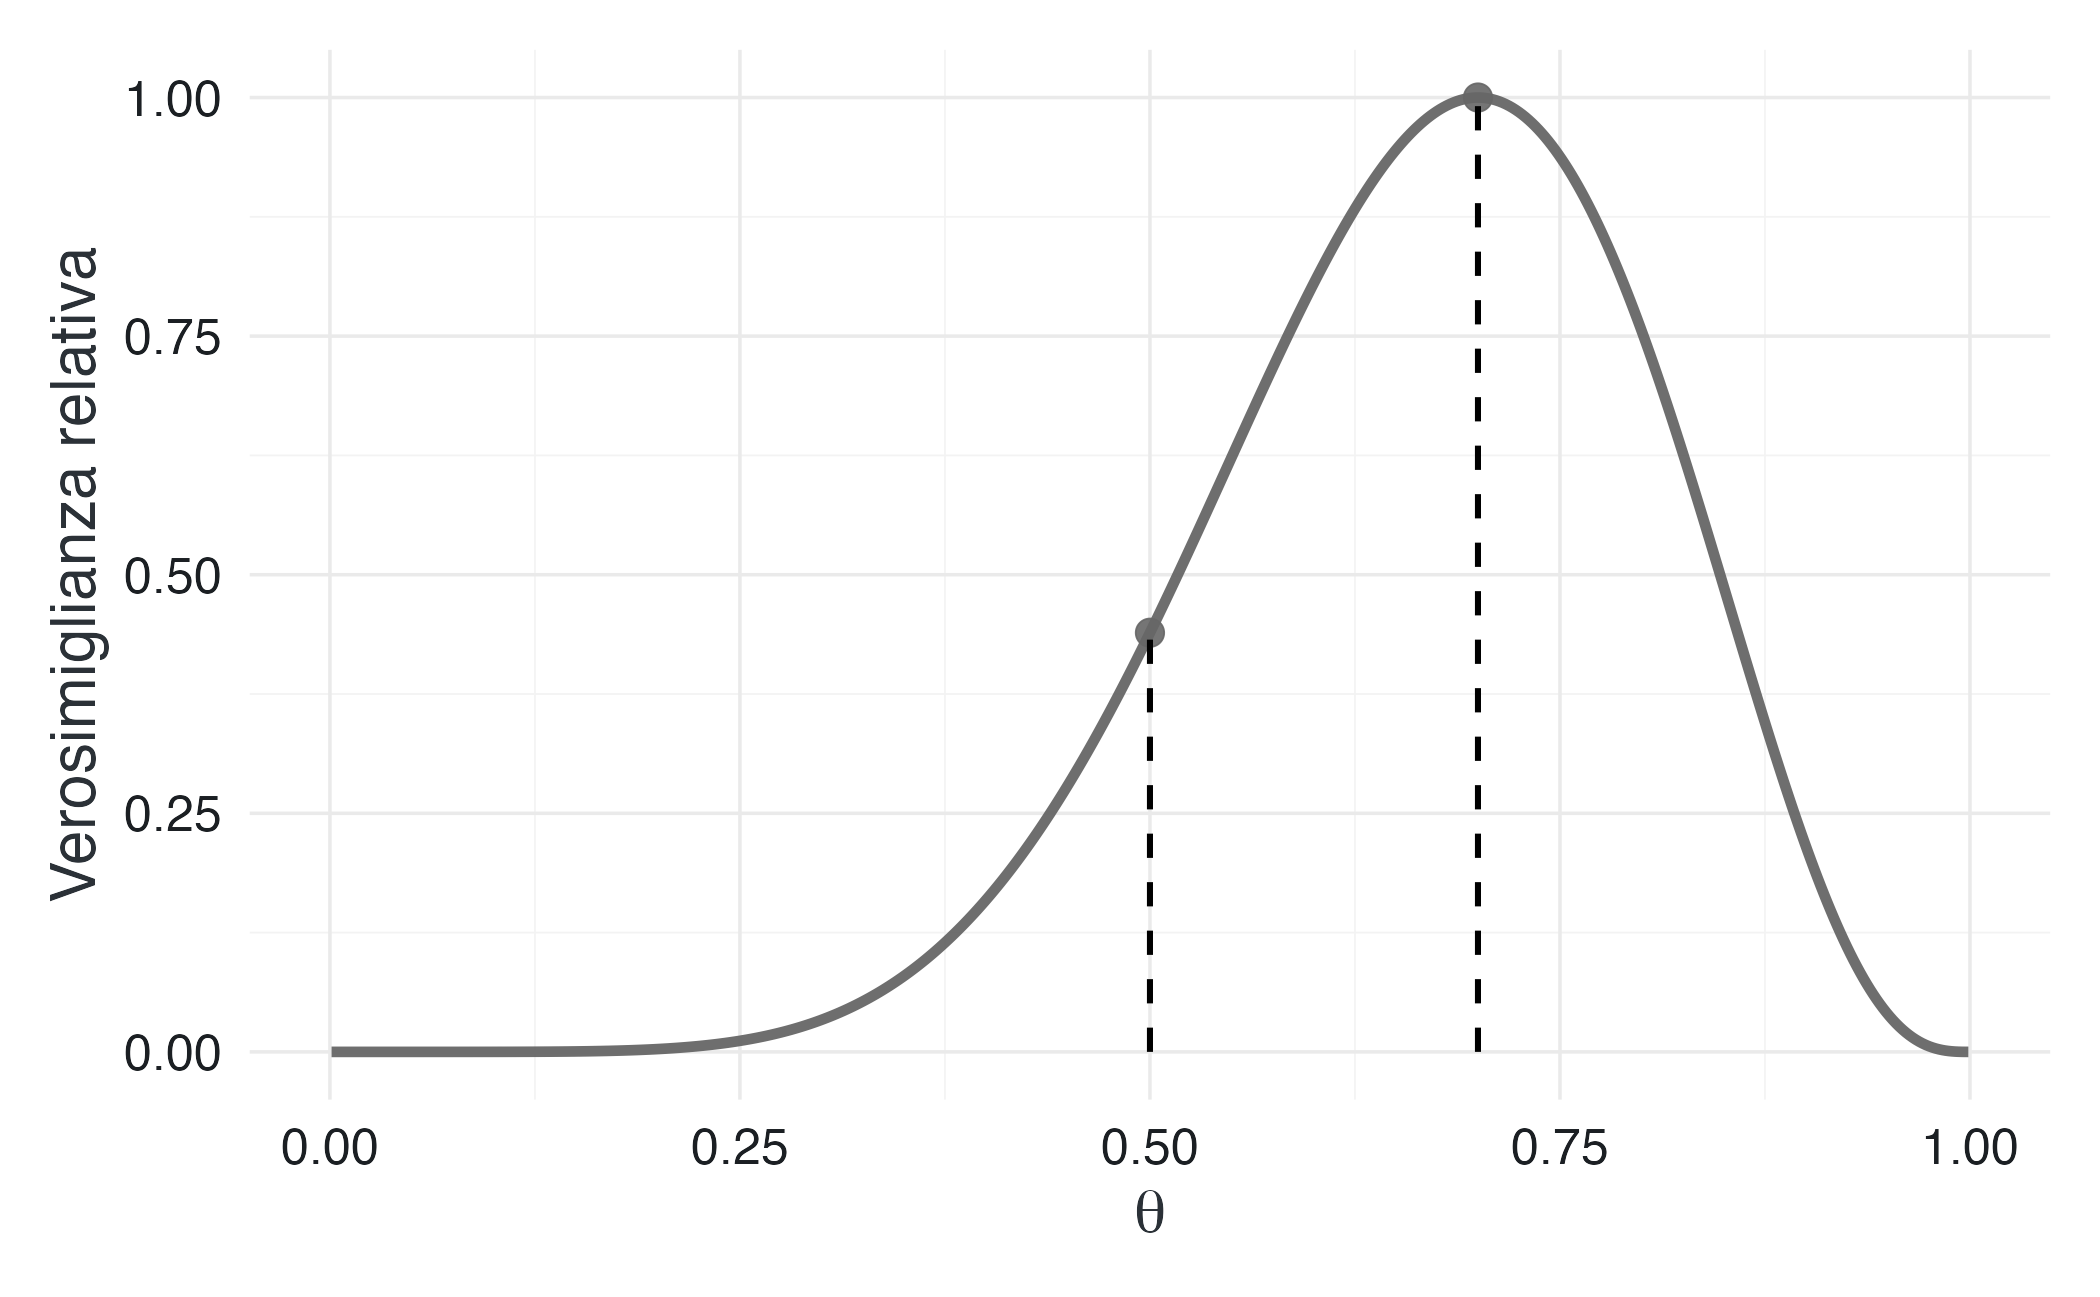
\includegraphics[width=0.85\linewidth,height=\textheight,keepaspectratio]{chapters/probability/14_likelihood_files/figure-pdf/fig-likelihood-ratio-1.png}

}

\caption{\label{fig-likelihood-ratio}Rapporto di verosimiglianza tra due
valori parametrici.}

\end{figure}%

\begin{tcolorbox}[enhanced jigsaw, arc=.35mm, bottomrule=.15mm, bottomtitle=1mm, breakable, colback=white, colbacktitle=quarto-callout-note-color!10!white, colframe=quarto-callout-note-color-frame, coltitle=black, left=2mm, leftrule=.75mm, opacityback=0, opacitybacktitle=0.6, rightrule=.15mm, title=\textcolor{quarto-callout-note-color}{\faInfo}\hspace{0.5em}{Connessione con il fattore di Bayes}, titlerule=0mm, toprule=.15mm, toptitle=1mm]

Nel confronto tra due ipotesi puntuali, se assegniamo uguali probabilità
a priori alle due ipotesi, il rapporto di verosimiglianza coincide con
il rapporto delle probabilità posteriori. Nei problemi più generali, il
confronto bayesiano tra modelli richiede la probabilità marginale dei
dati e conduce al fattore di Bayes.

\end{tcolorbox}

\section{Errori comuni nell'interpretazione della
verosimiglianza}\label{sec-likelihood-misinterpretations}

\subsection{Errore 1: scambiarla per la probabilità del
parametro}\label{errore-1-scambiarla-per-la-probabilituxe0-del-parametro}

La verosimiglianza non dice:

\[
P(\theta \mid y).
\]

Dice invece:

\[
p(y \mid \theta)
\]

vista come funzione di \(\theta\). La probabilità del parametro, nella
prospettiva bayesiana, è la posterior e richiede anche la prior.

\subsection{Errore 2: interpretare l'area sotto la curva come
probabilità}\label{errore-2-interpretare-larea-sotto-la-curva-come-probabilituxe0}

Una curva di verosimiglianza può assomigliare a una distribuzione, ma
l'area sotto la curva non ha automaticamente interpretazione
probabilistica. Prima bisogna moltiplicare per una prior e normalizzare.

\subsection{Errore 3: dimenticare il
modello}\label{errore-3-dimenticare-il-modello}

La verosimiglianza dipende dal modello scelto. Scrivere una
verosimiglianza binomiale significa assumere prove indipendenti, stessa
probabilità di successo per tutte le osservazioni e corretta definizione
di successo e insuccesso.

Se queste assunzioni sono sbagliate, la verosimiglianza può essere
precisa ma fuorviante. Questo riprende il tema del capitolo precedente:
la precisione statistica non garantisce accuratezza scientifica.

\subsection{Errore 4: trattare la MLE come conclusione
bayesiana}\label{errore-4-trattare-la-mle-come-conclusione-bayesiana}

La MLE è il valore che massimizza la verosimiglianza. Non incorpora
credenze pregresse, incertezza completa o distribuzioni a posteriori.
Può essere utile, ma non sostituisce l'aggiornamento bayesiano.

\begin{tcolorbox}[enhanced jigsaw, arc=.35mm, bottomrule=.15mm, bottomtitle=1mm, breakable, colback=white, colbacktitle=quarto-callout-warning-color!10!white, colframe=quarto-callout-warning-color-frame, coltitle=black, left=2mm, leftrule=.75mm, opacityback=0, opacitybacktitle=0.6, rightrule=.15mm, title=\textcolor{quarto-callout-warning-color}{\faExclamationTriangle}\hspace{0.5em}{Sintesi}, titlerule=0mm, toprule=.15mm, toptitle=1mm]

La verosimiglianza è indispensabile, ma non basta. Nell'inferenza
bayesiana completa, essa deve essere combinata con la prior e
normalizzata per ottenere la posterior.

\end{tcolorbox}

\section{Verso l'aggiornamento
bayesiano}\label{sec-likelihood-to-posterior}

A questo punto abbiamo tre elementi:

\begin{enumerate}
\def\labelenumi{\arabic{enumi}.}
\tightlist
\item
  un parametro ignoto \(\theta\);
\item
  una prior \(p(\theta)\) che rappresenta le credenze prima dei dati;
\item
  una verosimiglianza \(L(\theta; y)\) che rappresenta il supporto
  fornito dai dati.
\end{enumerate}

Il teorema di Bayes combina questi elementi:

\[
p(\theta \mid y)
= \frac{L(\theta; y)p(\theta)}{\int L(\theta'; y)p(\theta')\,d\theta'}.
\]

In forma proporzionale:

\[
p(\theta \mid y) \propto L(\theta; y)p(\theta).
\]

Questa formula esprime il ruolo della verosimiglianza nell'inferenza
bayesiana: essa \textbf{ribilancia} la prior, aumentando il peso dei
valori parametrici che rendono plausibili i dati e riducendo il peso di
quelli incompatibili con l'evidenza osservata.

Il prossimo capitolo approfondirà questo passaggio, mostrando come prior
e verosimiglianza si combinano in casi concreti e perché, con molti
dati, la posterior tende spesso a concentrarsi attorno ai valori meglio
supportati dall'evidenza.

\section*{Riflessioni conclusive}\label{riflessioni-conclusive-13}

\markright{Riflessioni conclusive}

La verosimiglianza formalizza il passaggio dal dato osservato
all'evidenza inferenziale. Essa risponde alla domanda: dato ciò che
abbiamo osservato, quali valori del parametro rendono quei dati più o
meno plausibili?

Il punto più importante è il cambio di prospettiva. Nel modello
generativo usiamo \(p(y \mid \theta)\) per descrivere i dati possibili
assumendo un parametro. Nella verosimiglianza fissiamo invece i dati
osservati e leggiamo la stessa quantità come funzione del parametro.
Questo cambio permette di confrontare valori alternativi di \(\theta\)
sulla base della loro compatibilità con l'evidenza.

Abbiamo visto che la verosimiglianza può essere costruita per dati
binomiali, per campioni indipendenti, per studi multipli e per dati
gaussiani. In tutti i casi, essa rende visibile quanta informazione i
dati portano: curve larghe indicano evidenza debole o imprecisa; curve
strette indicano evidenza più discriminante.

Dal punto di vista bayesiano, però, la verosimiglianza non è il punto di
arrivo. Non assegna probabilità ai parametri e non incorpora conoscenze
pregresse. Il suo ruolo è quello di collegare dati e credenze: nel
teorema di Bayes, la prior viene trasformata dalla verosimiglianza e
normalizzata nella posterior.

\section*{Punti chiave da ricordare}\label{punti-chiave-da-ricordare-13}
\addcontentsline{toc}{section}{Punti chiave da ricordare}

\markright{Punti chiave da ricordare}

\begin{tcolorbox}[enhanced jigsaw, arc=.35mm, bottomrule=.15mm, bottomtitle=1mm, breakable, colback=white, colbacktitle=quarto-callout-important-color!10!white, colframe=quarto-callout-important-color-frame, coltitle=black, left=2mm, leftrule=.75mm, opacityback=0, opacitybacktitle=0.6, rightrule=.15mm, title=\textcolor{quarto-callout-important-color}{\faExclamation}\hspace{0.5em}{Importante}, titlerule=0mm, toprule=.15mm, toptitle=1mm]

\begin{enumerate}
\def\labelenumi{\arabic{enumi}.}
\tightlist
\item
  \textbf{Cambio di prospettiva}

  \begin{itemize}
  \tightlist
  \item
    Probabilità: \(y\) varia, \(\theta\) è fissato.
  \item
    Verosimiglianza: \(y\) è fissato, \(\theta\) varia.
  \end{itemize}
\item
  \textbf{Definizione}

  \begin{itemize}
  \tightlist
  \item
    \(L(\theta; y_{obs}) = f(y_{obs}\mid\theta)\).
  \item
    Misura la compatibilità dei dati osservati con ciascun valore del
    parametro.
  \end{itemize}
\item
  \textbf{Non è una distribuzione sui parametri}

  \begin{itemize}
  \tightlist
  \item
    In generale non integra o somma a 1 rispetto a \(\theta\).
  \item
    Non va interpretata come \(p(\theta \mid y)\).
  \end{itemize}
\item
  \textbf{Scala relativa}

  \begin{itemize}
  \tightlist
  \item
    Costanti che non dipendono da \(\theta\) possono spesso essere
    ignorate.
  \item
    I rapporti di verosimiglianza sono più interpretabili dei valori
    assoluti.
  \end{itemize}
\item
  \textbf{Dati indipendenti}

  \begin{itemize}
  \tightlist
  \item
    Le verosimiglianze si moltiplicano.
  \item
    Le log-verosimiglianze si sommano.
  \end{itemize}
\item
  \textbf{Modello binomiale}

  \begin{itemize}
  \tightlist
  \item
    \(L(\theta; y,n) \propto \theta^y(1-\theta)^{n-y}\).
  \item
    Il massimo è in \(\hat{\theta}=y/n\).
  \item
    Campioni più grandi producono curve più concentrate.
  \end{itemize}
\item
  \textbf{Modello gaussiano}

  \begin{itemize}
  \tightlist
  \item
    Con varianza nota, la verosimiglianza per \(\mu\) è centrata su
    \(\bar{y}\).
  \item
    La sua varianza è \(\sigma^2/n\).
  \item
    La precisione dei dati è \(n/\sigma^2\).
  \end{itemize}
\item
  \textbf{Ruolo bayesiano}

  \begin{itemize}
  \tightlist
  \item
    La verosimiglianza è il contributo dei dati.
  \item
    La posterior nasce da prior \(\times\) verosimiglianza, seguita da
    normalizzazione.
  \end{itemize}
\end{enumerate}

\textbf{Formule essenziali:}

\[
L(\theta; y_{obs}) = f(y_{obs}\mid\theta).
\]

\[
L(\theta; y_1,\ldots,y_n)
= \prod_{i=1}^{n} f(y_i\mid\theta),
\qquad
\ell(\theta)=\sum_{i=1}^{n}\log f(y_i\mid\theta).
\]

\[
L(\theta; y,n) \propto \theta^y(1-\theta)^{n-y}
\qquad \text{(binomiale)}.
\]

\[
L(\mu; y_1,\ldots,y_n)
\propto
\exp\left[-\frac{n}{2\sigma^2}(\mu-\bar{y})^2\right]
\qquad \text{(normale con }\sigma\text{ nota)}.
\]

\[
p(\theta\mid y) \propto L(\theta; y)p(\theta).
\]

\textbf{Per il prossimo capitolo:}

Nel \textbf{?@sec-likelihood-properties} studieremo come la
verosimiglianza si combina con distribuzioni a priori specifiche, come
cambia la posterior al variare della forza dei dati e perché prior e
dati possono essere interpretati in termini di informazione e
precisione.

\end{tcolorbox}

\begin{tcolorbox}[enhanced jigsaw, arc=.35mm, bottomrule=.15mm, bottomtitle=1mm, breakable, colback=white, colbacktitle=quarto-callout-note-color!10!white, colframe=quarto-callout-note-color-frame, coltitle=black, left=2mm, leftrule=.75mm, opacityback=0, opacitybacktitle=0.6, rightrule=.15mm, title=\textcolor{quarto-callout-note-color}{\faInfo}\hspace{0.5em}{Informazioni sull'ambiente di sviluppo}, titlerule=0mm, toprule=.15mm, toptitle=1mm]

\begin{Shaded}
\begin{Highlighting}[]
\FunctionTok{sessionInfo}\NormalTok{()}
\CommentTok{\#\textgreater{} R version 4.6.1 (2026{-}06{-}24)}
\CommentTok{\#\textgreater{} Platform: aarch64{-}apple{-}darwin23}
\CommentTok{\#\textgreater{} Running under: macOS Tahoe 26.5.2}
\CommentTok{\#\textgreater{} }
\CommentTok{\#\textgreater{} Matrix products: default}
\CommentTok{\#\textgreater{} BLAS:   /Library/Frameworks/R.framework/Versions/4.6/Resources/lib/libRblas.0.dylib }
\CommentTok{\#\textgreater{} LAPACK: /Library/Frameworks/R.framework/Versions/4.6/Resources/lib/libRlapack.dylib;  LAPACK version 3.12.1}
\CommentTok{\#\textgreater{} }
\CommentTok{\#\textgreater{} locale:}
\CommentTok{\#\textgreater{} [1] C.UTF{-}8/UTF{-}8/C.UTF{-}8/C/C.UTF{-}8/C.UTF{-}8}
\CommentTok{\#\textgreater{} }
\CommentTok{\#\textgreater{} time zone: Europe/Rome}
\CommentTok{\#\textgreater{} tzcode source: internal}
\CommentTok{\#\textgreater{} }
\CommentTok{\#\textgreater{} attached base packages:}
\CommentTok{\#\textgreater{} [1] stats     graphics  grDevices utils     datasets  methods   base     }
\CommentTok{\#\textgreater{} }
\CommentTok{\#\textgreater{} other attached packages:}
\CommentTok{\#\textgreater{}  [1] ragg\_1.5.2            tinytable\_0.17.0      withr\_3.0.3          }
\CommentTok{\#\textgreater{}  [4] systemfonts\_1.3.2     patchwork\_1.3.2       ggdist\_3.3.3         }
\CommentTok{\#\textgreater{}  [7] tidybayes\_3.0.7       bayesplot\_1.15.0      ggplot2\_4.0.3        }
\CommentTok{\#\textgreater{} [10] reliabilitydiag\_0.2.1 priorsense\_1.2.0      posterior\_1.7.0      }
\CommentTok{\#\textgreater{} [13] loo\_2.10.0            rstan\_2.32.7          StanHeaders\_2.32.10  }
\CommentTok{\#\textgreater{} [16] brms\_2.23.0           Rcpp\_1.1.2            sessioninfo\_1.2.4    }
\CommentTok{\#\textgreater{} [19] conflicted\_1.2.0      janitor\_2.2.1         matrixStats\_1.5.0    }
\CommentTok{\#\textgreater{} [22] modelr\_0.1.11         tibble\_3.3.1          dplyr\_1.2.1          }
\CommentTok{\#\textgreater{} [25] tidyr\_1.3.2           rio\_1.3.0             here\_1.0.2           }
\CommentTok{\#\textgreater{} }
\CommentTok{\#\textgreater{} loaded via a namespace (and not attached):}
\CommentTok{\#\textgreater{}  [1] svUnit\_1.0.8          tidyselect\_1.2.1      farver\_2.1.2         }
\CommentTok{\#\textgreater{}  [4] S7\_0.2.2              fastmap\_1.2.0         tensorA\_0.36.2.1     }
\CommentTok{\#\textgreater{}  [7] digest\_0.6.39         timechange\_0.4.0      estimability\_2.0.0   }
\CommentTok{\#\textgreater{} [10] lifecycle\_1.0.5       magrittr\_2.0.5        compiler\_4.6.1       }
\CommentTok{\#\textgreater{} [13] rlang\_1.3.0           tools\_4.6.1           yaml\_2.3.12          }
\CommentTok{\#\textgreater{} [16] knitr\_1.51            labeling\_0.4.3        bridgesampling\_1.2{-}1 }
\CommentTok{\#\textgreater{} [19] pkgbuild\_1.4.8        curl\_7.1.0            RColorBrewer\_1.1{-}3   }
\CommentTok{\#\textgreater{} [22] abind\_1.4{-}8           purrr\_1.2.2           grid\_4.6.1           }
\CommentTok{\#\textgreater{} [25] stats4\_4.6.1          xtable\_1.8{-}8          inline\_0.3.21        }
\CommentTok{\#\textgreater{} [28] emmeans\_2.0.3         scales\_1.4.0          cli\_3.6.6            }
\CommentTok{\#\textgreater{} [31] mvtnorm\_1.4{-}1         rmarkdown\_2.31        generics\_0.1.4       }
\CommentTok{\#\textgreater{} [34] otel\_0.2.0            RcppParallel\_5.1.11{-}2 cachem\_1.1.0         }
\CommentTok{\#\textgreater{} [37] stringr\_1.6.0         parallel\_4.6.1        vctrs\_0.7.3          }
\CommentTok{\#\textgreater{} [40] V8\_8.2.0              Matrix\_1.7{-}5          jsonlite\_2.0.0       }
\CommentTok{\#\textgreater{} [43] arrayhelpers\_1.1{-}1    glue\_1.8.1            codetools\_0.2{-}20     }
\CommentTok{\#\textgreater{} [46] distributional\_0.8.1  lubridate\_1.9.5       stringi\_1.8.7        }
\CommentTok{\#\textgreater{} [49] gtable\_0.3.6          QuickJSR\_1.10.0       pillar\_1.11.1        }
\CommentTok{\#\textgreater{} [52] htmltools\_0.5.9       Brobdingnag\_1.2{-}9     R6\_2.6.1             }
\CommentTok{\#\textgreater{} [55] textshaping\_1.0.5     rprojroot\_2.1.1       evaluate\_1.0.5       }
\CommentTok{\#\textgreater{} [58] lattice\_0.22{-}9        backports\_1.5.1       memoise\_2.0.1        }
\CommentTok{\#\textgreater{} [61] broom\_1.0.13          snakecase\_0.11.1      rstantools\_2.6.0     }
\CommentTok{\#\textgreater{} [64] coda\_0.19{-}4.1         gridExtra\_2.3.1       nlme\_3.1{-}169         }
\CommentTok{\#\textgreater{} [67] checkmate\_2.3.4       xfun\_0.60             pkgconfig\_2.0.3}
\end{Highlighting}
\end{Shaded}

\end{tcolorbox}

\section*{Bibliografia}\label{bibliografia-8}

\markright{Bibliografia}

\chapter{Dalla verosimiglianza alla posterior: l'aggiornamento
bayesiano}\label{sec-bayesian-updating}

\section*{Introduzione}\label{introduzione-14}

\markright{Introduzione}

Nel Capitolo~\ref{sec-prob-inference-uncertainty} abbiamo discusso come
un campione possa essere più o meno informativo: i campioni piccoli
producono evidenze instabili, mentre i campioni più grandi tendono a
fornire stime più precise. È importante distinguere l'incertezza
campionaria dalle eventuali distorsioni sistematiche. Nel
Capitolo~\ref{sec-prob-likelihood} abbiamo poi introdotto la
\textbf{verosimiglianza}, ovvero la funzione che misura quanto i dati
osservati siano compatibili con i possibili valori del parametro.

Resta ora il passaggio propriamente bayesiano: \textbf{come usiamo la
verosimiglianza per aggiornare una credenza a priori?}

A questa domanda risponde il presente capitolo. La sua funzione non è
quella di ripetere le proprietà della media campionaria, della Legge dei
Grandi Numeri o del Teorema del Limite Centrale. Quei concetti hanno già
preparato il terreno. Qui ci concentriamo invece sulla trasformazione
fondamentale dell'inferenza bayesiana:

\[
\text{prior} \times \text{verosimiglianza} \longrightarrow \text{posterior}.
\]

L'idea centrale è semplice: prima di osservare i dati, rappresentiamo la
nostra incertezza su un parametro tramite una distribuzione \emph{a
priori}. I dati producono una funzione di verosimiglianza. Il prodotto
tra queste due componenti, opportunamente normalizzato, produce una
nuova distribuzione: la distribuzione \emph{a posteriori}.

In questo capitolo:

\begin{enumerate}
\def\labelenumi{\arabic{enumi}.}
\tightlist
\item
  \textbf{chiariremo} il ruolo di prior, verosimiglianza, evidenza
  marginale e posterior;
\item
  \textbf{studieremo} l'esempio Beta-Binomiale, adatto a proporzioni e
  prevalenze;
\item
  \textbf{useremo} l'analisi di sensibilità per valutare quanto le
  conclusioni dipendano dalla prior;
\item
  \textbf{esamineremo} il caso Normale-Normale, in cui l'aggiornamento
  assume la forma di una media pesata dalle precisioni;
\item
  \textbf{mostreremo} l'aggiornamento sequenziale, in cui la posterior
  di oggi diventa la prior di domani;
\item
  \textbf{discuteremo} brevemente cosa la posterior può e non può dirci.
\end{enumerate}

\begin{tcolorbox}[enhanced jigsaw, arc=.35mm, bottomrule=.15mm, bottomtitle=1mm, breakable, colback=white, colbacktitle=quarto-callout-tip-color!10!white, colframe=quarto-callout-tip-color-frame, coltitle=black, left=2mm, leftrule=.75mm, opacityback=0, opacitybacktitle=0.6, rightrule=.15mm, title=\textcolor{quarto-callout-tip-color}{\faLightbulb}\hspace{0.5em}{Prerequisiti}, titlerule=0mm, toprule=.15mm, toptitle=1mm]

Per seguire questo capitolo è utile aver letto:

\begin{itemize}
\tightlist
\item
  Capitolo~\ref{sec-prob-bayes-theorem} -- per il teorema di Bayes;
\item
  Capitolo~\ref{sec-prob-inference-uncertainty} -- per informazione,
  precisione e incertezza campionaria;
\item
  2 -- per Bernoulli, Binomiale e Beta;
\item
  Capitolo~\ref{sec-prob-cont-distr} -- per la distribuzione Normale;
\item
  Capitolo~\ref{sec-prob-likelihood} -- fondamentale per il concetto di
  verosimiglianza.
\end{itemize}

Questo capitolo conclude il passaggio dalla probabilità alla logica
dell'inferenza bayesiana parametrica.

\end{tcolorbox}

\begin{tcolorbox}[enhanced jigsaw, arc=.35mm, bottomrule=.15mm, bottomtitle=1mm, breakable, colback=white, colbacktitle=quarto-callout-caution-color!10!white, colframe=quarto-callout-caution-color-frame, coltitle=black, left=2mm, leftrule=.75mm, opacityback=0, opacitybacktitle=0.6, rightrule=.15mm, title=\textcolor{quarto-callout-caution-color}{\faFire}\hspace{0.5em}{Preparazione del Notebook}, titlerule=0mm, toprule=.15mm, toptitle=1mm]

\begin{Shaded}
\begin{Highlighting}[]
\ControlFlowTok{if}\NormalTok{ (}\FunctionTok{requireNamespace}\NormalTok{(}\StringTok{"here"}\NormalTok{, }\AttributeTok{quietly =} \ConstantTok{TRUE}\NormalTok{) }\SpecialCharTok{\&\&}
    \FunctionTok{file.exists}\NormalTok{(here}\SpecialCharTok{::}\FunctionTok{here}\NormalTok{(}\StringTok{"code"}\NormalTok{, }\StringTok{"\_common.R"}\NormalTok{))) \{}
  \FunctionTok{source}\NormalTok{(here}\SpecialCharTok{::}\FunctionTok{here}\NormalTok{(}\StringTok{"code"}\NormalTok{, }\StringTok{"\_common.R"}\NormalTok{))}
\NormalTok{\}}

\ControlFlowTok{if}\NormalTok{ (}\FunctionTok{exists}\NormalTok{(}\StringTok{"apply\_visual\_theme"}\NormalTok{)) \{}
  \FunctionTok{apply\_visual\_theme}\NormalTok{()}
\NormalTok{\}}
\end{Highlighting}
\end{Shaded}

\end{tcolorbox}

\section{Perchè serve ancora un capitolo dopo la
verosimiglianza?}\label{sec-why-posterior-after-likelihood}

La verosimiglianza risponde a una domanda precisa:

\begin{quote}
Dati i valori osservati, quali valori del parametro rendono questi dati
più o meno plausibili?
\end{quote}

Questa domanda è essenziale, ma non esaurisce l'inferenza bayesiana. La
verosimiglianza, da sola, non costituisce ancora una distribuzione di
probabilità sul parametro. Non risponde direttamente alla domanda:
``Qual è la probabilità che il parametro sia in un certo intervallo?''.
Per rispondere a questa domanda, è necessario combinare la
verosimiglianza con una distribuzione a priori.

In termini bayesiani, il parametro non è trattato come una quantità
casuale perché cambia da un esperimento all'altro, ma perché è
\textbf{ignoto}. La probabilità rappresenta il nostro stato di
informazione su quel parametro.

Prima dei dati:

\[
\theta \sim p(\theta).
\]

Dopo i dati:

\[
\theta \mid y \sim p(\theta \mid y).
\]

Il compito del presente capitolo è spiegare come si passa dalla prima
distribuzione alla seconda.

\begin{tcolorbox}[enhanced jigsaw, arc=.35mm, bottomrule=.15mm, bottomtitle=1mm, breakable, colback=white, colbacktitle=quarto-callout-note-color!10!white, colframe=quarto-callout-note-color-frame, coltitle=black, left=2mm, leftrule=.75mm, opacityback=0, opacitybacktitle=0.6, rightrule=.15mm, title=\textcolor{quarto-callout-note-color}{\faInfo}\hspace{0.5em}{Tre ruoli distinti}, titlerule=0mm, toprule=.15mm, toptitle=1mm]

Nel percorso del manuale, i tre capitoli hanno funzioni diverse:

\begin{itemize}
\tightlist
\item
  il Capitolo~\ref{sec-prob-inference-uncertainty} spiega \textbf{quanto
  sono informativi i dati};
\item
  il Capitolo~\ref{sec-prob-likelihood} spiega \textbf{come
  rappresentiamo l'informazione dei dati};
\item
  questo capitolo spiega \textbf{come l'informazione dei dati aggiorna
  le credenze}.
\end{itemize}

\end{tcolorbox}

\section{La regola di aggiornamento
bayesiano}\label{sec-bayes-update-rule}

\subsection{Forma generale}\label{forma-generale}

Sia \(\theta\) il parametro di interesse e siano \(y\) i dati osservati.
La regola di Bayes si scrive:

\[
p(\theta \mid y) =
\frac{p(y \mid \theta)p(\theta)}{p(y)}.
\]

I quattro termini hanno ruoli diversi:

\begin{itemize}
\tightlist
\item
  \(p(\theta)\) è la \textbf{prior}, cioè la distribuzione che
  rappresenta l'incertezza prima dei dati;
\item
  \(p(y \mid \theta)\) è la \textbf{verosimiglianza}, cioè la
  compatibilità dei dati con ciascun valore del parametro;
\item
  \(p(y)\) è l'\textbf{evidenza marginale}, cioè la costante che rende
  la posterior una vera distribuzione di probabilità;
\item
  \(p(\theta \mid y)\) è la \textbf{posterior}, cioè la distribuzione
  aggiornata dopo aver osservato i dati.
\end{itemize}

Poichè \(p(y)\) non dipende da \(\theta\), spesso scriviamo:

\[
p(\theta \mid y) \propto p(y \mid \theta)p(\theta).
\]

Questa forma proporzionale è la più importante da ricordare.

\begin{tcolorbox}[enhanced jigsaw, arc=.35mm, bottomrule=.15mm, bottomtitle=1mm, breakable, colback=white, colbacktitle=quarto-callout-important-color!10!white, colframe=quarto-callout-important-color-frame, coltitle=black, left=2mm, leftrule=.75mm, opacityback=0, opacitybacktitle=0.6, rightrule=.15mm, title=\textcolor{quarto-callout-important-color}{\faExclamation}\hspace{0.5em}{Importante}, titlerule=0mm, toprule=.15mm, toptitle=1mm]

La posterior non è semplicemente la verosimiglianza. È la
verosimiglianza \textbf{ponderata} dalla prior e poi normalizzata
affinché l'area totale sia uguale a 1.

\end{tcolorbox}

\subsection{Il ruolo della costante di
normalizzazione}\label{il-ruolo-della-costante-di-normalizzazione}

Nel caso continuo, l'evidenza marginale è un integrale:

\[
p(y) = \int p(y \mid \theta)p(\theta)\,d\theta.
\]

Nel caso discreto, è una somma:

\[
p(y) = \sum_{\theta} p(y \mid \theta)p(\theta).
\]

Questo termine ha una funzione tecnica ma fondamentale: trasforma il
prodotto \(p(y \mid \theta)p(\theta)\) in una distribuzione di
probabilità valida. Senza questa normalizzazione, otterremmo una curva
proporzionale alla posterior, ma non una distribuzione con area totale
pari a 1.

\section{Esempio Beta-Binomiale: prevalenza di sintomi
depressivi}\label{sec-beta-binomial-update}

\subsection{Il problema}\label{il-problema-1}

Supponiamo di voler stimare la proporzione di studenti universitari con
sintomi depressivi clinicamente rilevanti, indicata con il simbolo
\(\theta\). In uno studio osserviamo:

\[
y = 72
\qquad \text{studenti con sintomi su} \qquad
n = 200.
\]

La proporzione osservata è:

\[
\hat{p} = \frac{72}{200} = 0.36.
\]

Nel capitolo sulla verosimiglianza abbiamo visto che, per dati binari,
il modello naturale è:

\[
Y \mid \theta \sim \text{Binomiale}(n, \theta).
\]

La verosimiglianza è:

\[
p(y \mid \theta) = \binom{n}{y}\theta^y(1-\theta)^{n-y}.
\]

Ora aggiungiamo l'elemento bayesiano: una prior su \(\theta\).

\subsection{La prior Beta}\label{la-prior-beta}

Per una proporzione, la distribuzione Beta è una scelta naturale per la
prior, perché è definita sull'intervallo \([0,1]\):

\[
\theta \sim \text{Beta}(\alpha, \beta).
\]

La densità della prior è proporzionale a:

\[
p(\theta) \propto \theta^{\alpha - 1}(1-\theta)^{\beta - 1}.
\]

I parametri \(\alpha\) e \(\beta\) controllano la forma della
distribuzione. Una lettura utile, anche se solo intuitiva, è considerare
\(\alpha\) e \(\beta\) come a una sorta di informazione precedente sui
successi e gli insuccessi.

Per esempio:

\begin{itemize}
\tightlist
\item
  \(\text{Beta}(1,1)\) è uniforme: tutti i valori di \(\theta\) sono
  ugualmente plausibili prima dei dati;
\item
  \(\text{Beta}(2,8)\) assegna più massa a valori bassi della
  proporzione;
\item
  \(\text{Beta}(8,2)\) assegna più massa a valori alti della
  proporzione.
\end{itemize}

\subsection{Prior, verosimiglianza e
posterior}\label{prior-verosimiglianza-e-posterior}

Se la prior è Beta e la verosimiglianza è Binomiale, la posterior è
ancora Beta:

\[
\theta \mid y \sim \text{Beta}(\alpha + y,\; \beta + n - y).
\]

Questa è una relazione particolarmente trasparente. I dati aggiornano i
parametri della prior aggiungendo:

\begin{itemize}
\tightlist
\item
  \(y\) successi al parametro \(\alpha\);
\item
  \(n-y\) insuccessi al parametro \(\beta\).
\end{itemize}

\begin{tcolorbox}[enhanced jigsaw, arc=.35mm, bottomrule=.15mm, bottomtitle=1mm, breakable, colback=white, colbacktitle=quarto-callout-note-color!10!white, colframe=quarto-callout-note-color-frame, coltitle=black, left=2mm, leftrule=.75mm, opacityback=0, opacitybacktitle=0.6, rightrule=.15mm, title=\textcolor{quarto-callout-note-color}{\faInfo}\hspace{0.5em}{Coniugazione}, titlerule=0mm, toprule=.15mm, toptitle=1mm]

Quando la prior e la verosimiglianza producono una posterior della
stessa famiglia della prior, si parla di \textbf{prior coniugato}. Nel
caso Beta-Binomiale, la prior Beta è coniugata alla verosimiglianza
Binomiale.

\end{tcolorbox}

\subsection{Esempio numerico}\label{esempio-numerico-1}

Usiamo una prior debolmente informativa:

\[
\theta \sim \text{Beta}(2,2).
\]

Dopo aver osservato \(y=72\) studenti con sintomi su \(n=200\), la
posterior è:

\[
\theta \mid y \sim \text{Beta}(2+72,\; 2+128)
= \text{Beta}(74,130).
\]

\begin{Shaded}
\begin{Highlighting}[]
\NormalTok{alpha\_prior }\OtherTok{\textless{}{-}} \DecValTok{2}
\NormalTok{beta\_prior }\OtherTok{\textless{}{-}} \DecValTok{2}
\NormalTok{n }\OtherTok{\textless{}{-}} \DecValTok{200}
\NormalTok{y }\OtherTok{\textless{}{-}} \DecValTok{72}

\NormalTok{alpha\_post }\OtherTok{\textless{}{-}}\NormalTok{ alpha\_prior }\SpecialCharTok{+}\NormalTok{ y}
\NormalTok{beta\_post }\OtherTok{\textless{}{-}}\NormalTok{ beta\_prior }\SpecialCharTok{+}\NormalTok{ n }\SpecialCharTok{{-}}\NormalTok{ y}

\NormalTok{theta\_grid }\OtherTok{\textless{}{-}} \FunctionTok{seq}\NormalTok{(}\FloatTok{0.001}\NormalTok{, }\FloatTok{0.999}\NormalTok{, }\AttributeTok{length.out =} \DecValTok{1000}\NormalTok{)}
\NormalTok{prior\_density }\OtherTok{\textless{}{-}} \FunctionTok{dbeta}\NormalTok{(theta\_grid, alpha\_prior, beta\_prior)}
\NormalTok{likelihood }\OtherTok{\textless{}{-}} \FunctionTok{dbinom}\NormalTok{(y, }\AttributeTok{size =}\NormalTok{ n, }\AttributeTok{prob =}\NormalTok{ theta\_grid)}
\NormalTok{posterior\_density }\OtherTok{\textless{}{-}} \FunctionTok{dbeta}\NormalTok{(theta\_grid, alpha\_post, beta\_post)}

\CommentTok{\# La verosimiglianza viene riscalata solo per confronto grafico.}
\NormalTok{likelihood\_scaled }\OtherTok{\textless{}{-}}\NormalTok{ likelihood }\SpecialCharTok{*} \FunctionTok{max}\NormalTok{(prior\_density) }\SpecialCharTok{/} \FunctionTok{max}\NormalTok{(likelihood)}

\NormalTok{plot\_data }\OtherTok{\textless{}{-}} \FunctionTok{data.frame}\NormalTok{(}
  \AttributeTok{theta =} \FunctionTok{rep}\NormalTok{(theta\_grid, }\DecValTok{3}\NormalTok{),}
  \AttributeTok{density =} \FunctionTok{c}\NormalTok{(prior\_density, likelihood\_scaled, posterior\_density),}
  \AttributeTok{componente =} \FunctionTok{factor}\NormalTok{(}
    \FunctionTok{rep}\NormalTok{(}\FunctionTok{c}\NormalTok{(}\StringTok{"Prior"}\NormalTok{, }\StringTok{"Verosimiglianza (riscalata)"}\NormalTok{, }\StringTok{"Posterior"}\NormalTok{),}
        \AttributeTok{each =} \FunctionTok{length}\NormalTok{(theta\_grid)),}
    \AttributeTok{levels =} \FunctionTok{c}\NormalTok{(}\StringTok{"Prior"}\NormalTok{, }\StringTok{"Verosimiglianza (riscalata)"}\NormalTok{, }\StringTok{"Posterior"}\NormalTok{)}
\NormalTok{  )}
\NormalTok{)}

\FunctionTok{ggplot}\NormalTok{(plot\_data, }\FunctionTok{aes}\NormalTok{(}\AttributeTok{x =}\NormalTok{ theta, }\AttributeTok{y =}\NormalTok{ density,}
                      \AttributeTok{color =}\NormalTok{ componente, }\AttributeTok{linetype =}\NormalTok{ componente)) }\SpecialCharTok{+}
  \FunctionTok{geom\_line}\NormalTok{(}\AttributeTok{linewidth =} \FloatTok{1.1}\NormalTok{) }\SpecialCharTok{+}
  \FunctionTok{geom\_vline}\NormalTok{(}\AttributeTok{xintercept =}\NormalTok{ y }\SpecialCharTok{/}\NormalTok{ n, }\AttributeTok{linetype =} \StringTok{"dashed"}\NormalTok{) }\SpecialCharTok{+}
  \FunctionTok{labs}\NormalTok{(}
    \AttributeTok{x =} \FunctionTok{expression}\NormalTok{(theta),}
    \AttributeTok{y =} \StringTok{"Densità / scala relativa"}\NormalTok{,}
    \AttributeTok{color =} \StringTok{""}\NormalTok{,}
    \AttributeTok{linetype =} \StringTok{""}
\NormalTok{  ) }\SpecialCharTok{+}
  \FunctionTok{theme}\NormalTok{(}\AttributeTok{legend.position =} \StringTok{"bottom"}\NormalTok{)}
\end{Highlighting}
\end{Shaded}

\begin{figure}[H]

\centering{

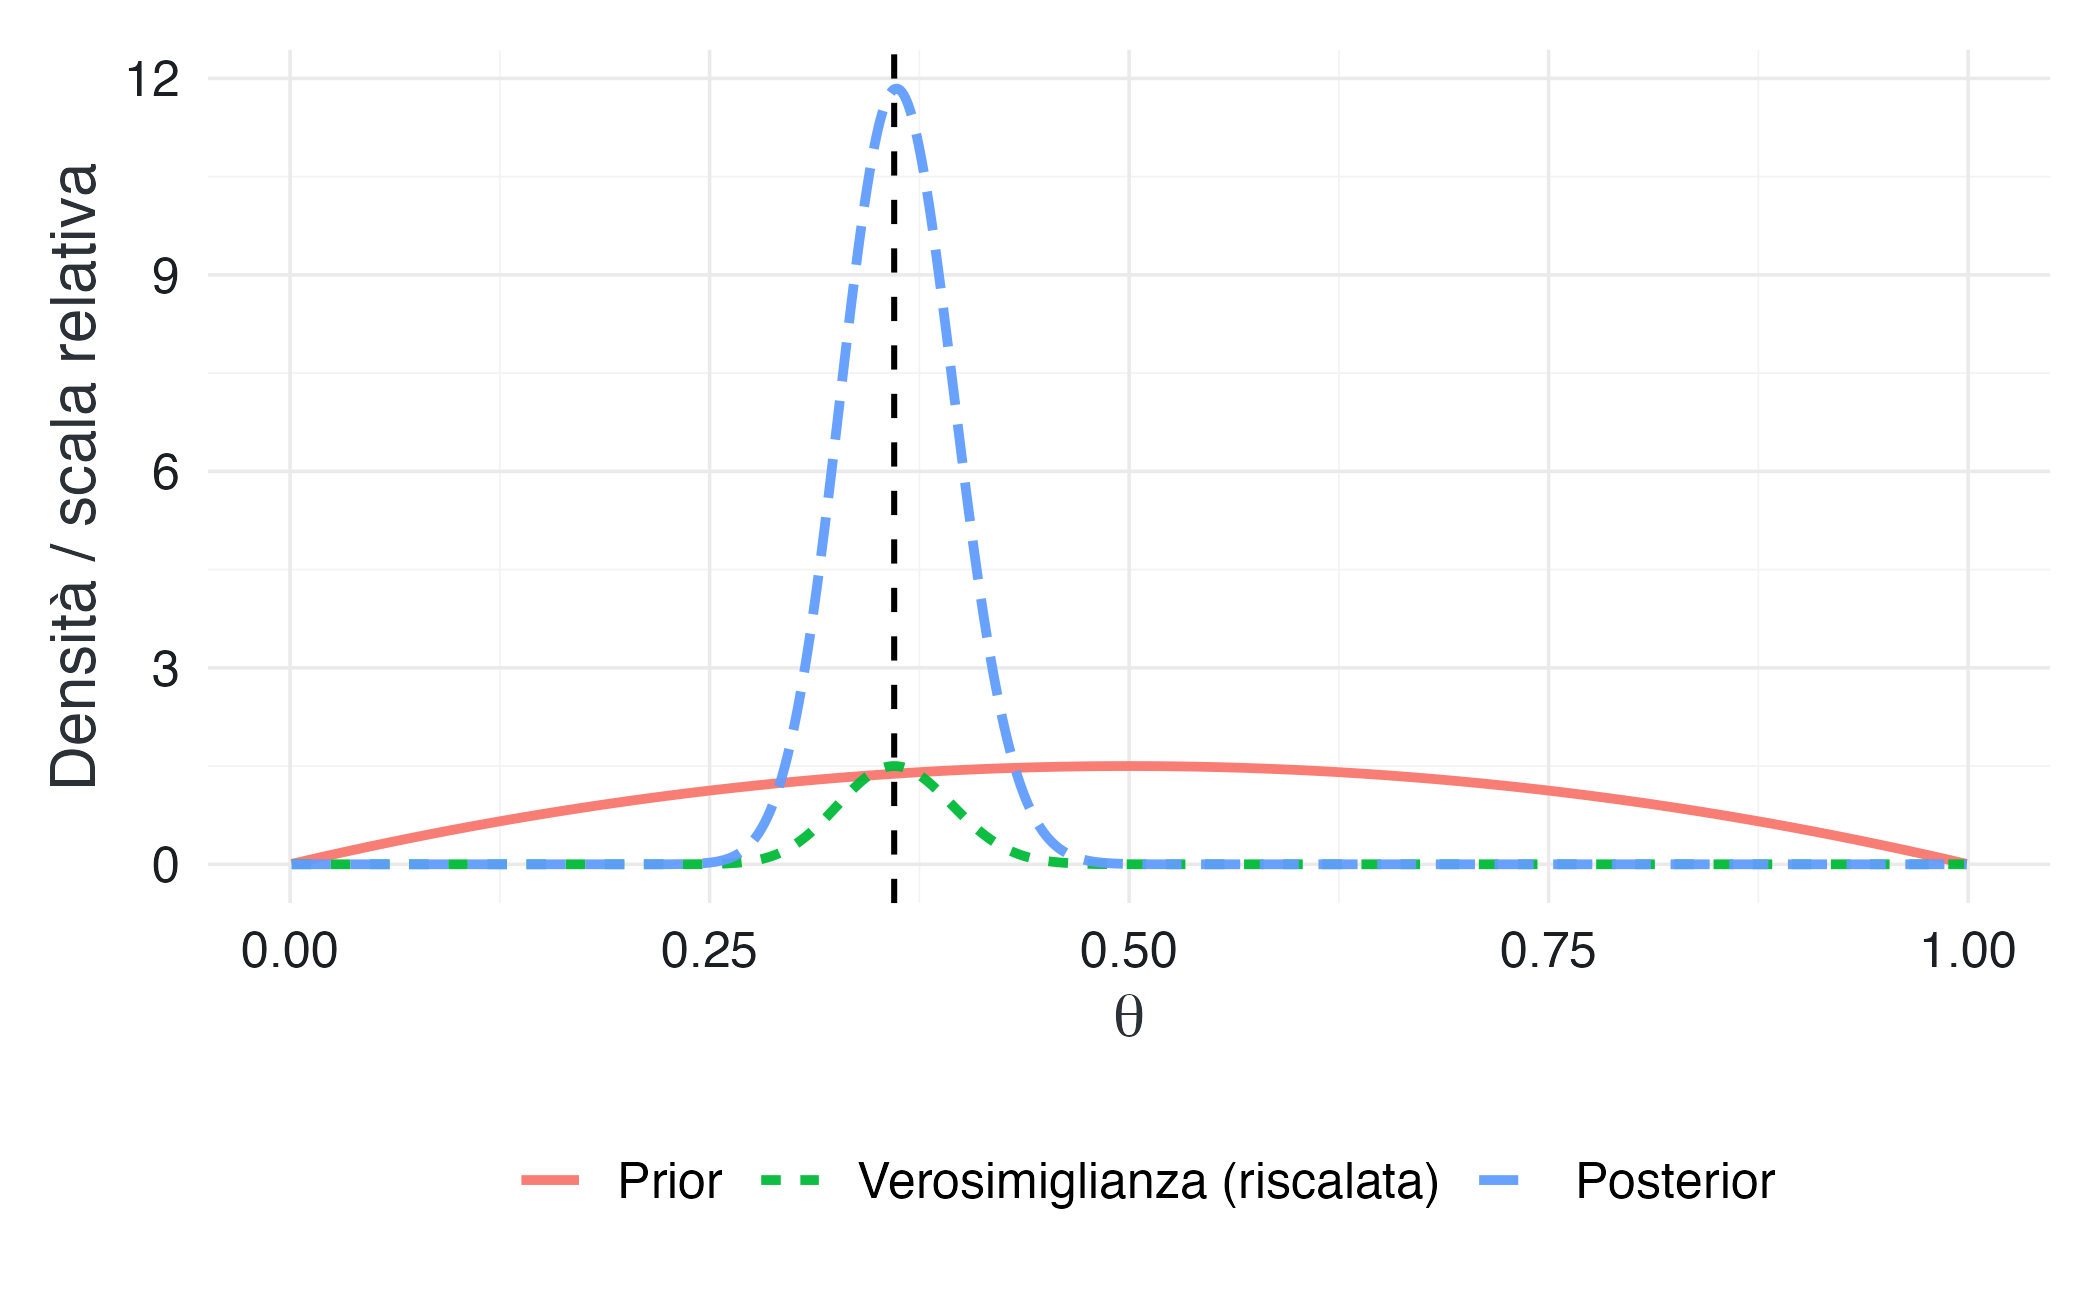
\includegraphics[width=0.85\linewidth,height=\textheight,keepaspectratio]{chapters/probability/15_aggiornamento_bayesiano_files/figure-pdf/fig-beta-binomial-update-1.png}

}

\caption{\label{fig-beta-binomial-update}Aggiornamento Beta-Binomiale:
prior, verosimiglianza normalizzata e posterior. La posterior combina
l'informazione iniziale con l'evidenza osservata.}

\end{figure}%

\begin{Shaded}
\begin{Highlighting}[]
\NormalTok{post\_mean }\OtherTok{\textless{}{-}}\NormalTok{ alpha\_post }\SpecialCharTok{/}\NormalTok{ (alpha\_post }\SpecialCharTok{+}\NormalTok{ beta\_post)}
\NormalTok{post\_ci }\OtherTok{\textless{}{-}} \FunctionTok{qbeta}\NormalTok{(}\FunctionTok{c}\NormalTok{(}\FloatTok{0.025}\NormalTok{, }\FloatTok{0.975}\NormalTok{), alpha\_post, beta\_post)}

\FunctionTok{cat}\NormalTok{(}\StringTok{"Prior: Beta("}\NormalTok{, alpha\_prior, }\StringTok{", "}\NormalTok{, beta\_prior, }\StringTok{")}\SpecialCharTok{\textbackslash{}n}\StringTok{"}\NormalTok{, }\AttributeTok{sep =} \StringTok{""}\NormalTok{)}
\CommentTok{\#\textgreater{} Prior: Beta(2, 2)}
\FunctionTok{cat}\NormalTok{(}\StringTok{"Dati: y ="}\NormalTok{, y, }\StringTok{"su n ="}\NormalTok{, n, }\StringTok{"}\SpecialCharTok{\textbackslash{}n}\StringTok{"}\NormalTok{)}
\CommentTok{\#\textgreater{} Dati: y = 72 su n = 200}
\FunctionTok{cat}\NormalTok{(}\StringTok{"Posterior: Beta("}\NormalTok{, alpha\_post, }\StringTok{", "}\NormalTok{, beta\_post, }\StringTok{")}\SpecialCharTok{\textbackslash{}n}\StringTok{"}\NormalTok{, }\AttributeTok{sep =} \StringTok{""}\NormalTok{)}
\CommentTok{\#\textgreater{} Posterior: Beta(74, 130)}
\FunctionTok{cat}\NormalTok{(}\StringTok{"Media posterior:"}\NormalTok{, }\FunctionTok{round}\NormalTok{(post\_mean, }\DecValTok{3}\NormalTok{), }\StringTok{"}\SpecialCharTok{\textbackslash{}n}\StringTok{"}\NormalTok{)}
\CommentTok{\#\textgreater{} Media posterior: 0.363}
\FunctionTok{cat}\NormalTok{(}\StringTok{"Intervallo di credibilità 95\%: ["}\NormalTok{,}
    \FunctionTok{round}\NormalTok{(post\_ci[}\DecValTok{1}\NormalTok{], }\DecValTok{3}\NormalTok{), }\StringTok{", "}\NormalTok{, }\FunctionTok{round}\NormalTok{(post\_ci[}\DecValTok{2}\NormalTok{], }\DecValTok{3}\NormalTok{), }\StringTok{"]}\SpecialCharTok{\textbackslash{}n}\StringTok{"}\NormalTok{, }\AttributeTok{sep =} \StringTok{""}\NormalTok{)}
\CommentTok{\#\textgreater{} Intervallo di credibilità 95\%: [0.298, 0.43]}
\end{Highlighting}
\end{Shaded}

\subsection{Come interpretare la
posterior}\label{come-interpretare-la-posterior}

La posterior è una distribuzione di probabilità su \(\theta\) dopo aver
osservato i dati. Possiamo quindi fare affermazioni del tipo:

\[
P(\theta > 0.40 \mid y).
\]

Questa è una probabilità bayesiana diretta: condizionatamente al
modello, alla prior e ai dati osservati, quantifica quanto sia
plausibile che la prevalenza superi il 40\%.

\begin{Shaded}
\begin{Highlighting}[]
\NormalTok{prob\_greater\_40 }\OtherTok{\textless{}{-}} \DecValTok{1} \SpecialCharTok{{-}} \FunctionTok{pbeta}\NormalTok{(}\FloatTok{0.40}\NormalTok{, alpha\_post, beta\_post)}
\FunctionTok{cat}\NormalTok{(}\StringTok{"P(theta \textgreater{} 0.40 | dati) ="}\NormalTok{, }\FunctionTok{round}\NormalTok{(prob\_greater\_40, }\DecValTok{3}\NormalTok{), }\StringTok{"}\SpecialCharTok{\textbackslash{}n}\StringTok{"}\NormalTok{)}
\CommentTok{\#\textgreater{} P(theta \textgreater{} 0.40 | dati) = 0.135}
\end{Highlighting}
\end{Shaded}

\begin{tcolorbox}[enhanced jigsaw, arc=.35mm, bottomrule=.15mm, bottomtitle=1mm, breakable, colback=white, colbacktitle=quarto-callout-important-color!10!white, colframe=quarto-callout-important-color-frame, coltitle=black, left=2mm, leftrule=.75mm, opacityback=0, opacitybacktitle=0.6, rightrule=.15mm, title=\textcolor{quarto-callout-important-color}{\faExclamation}\hspace{0.5em}{Importante}, titlerule=0mm, toprule=.15mm, toptitle=1mm]

Un intervallo di credibilità non ha la stessa interpretazione di un
intervallo di confidenza frequentista. Un intervallo di credibilità al
95\% contiene il 95\% della massa della distribuzione a posteriori, dato
il modello, la prior e i dati osservati.

\end{tcolorbox}

\section{Analisi di sensibilità al prior}\label{sec-prior-sensitivity}

La prior è parte del modello. Per questo motivo è buona pratica
chiedersi se le conclusioni cambiano in modo sostanziale quando si
scelgono prior ragionevoli ma diverse.

Questa verifica prende il nome di \textbf{analisi di sensibilità}.

La domanda non è:

\begin{quote}
Quale prior è l'unica corretta?
\end{quote}

La domanda è:

\begin{quote}
Le conclusioni principali dipendono in modo fragile da una particolare
scelta della prior?
\end{quote}

\subsection{Confronto tra prior
diverse}\label{confronto-tra-prior-diverse}

Consideriamo gli stessi dati:

\[
y = 72, \qquad n = 200.
\]

Confrontiamo quattro prior:

\begin{itemize}
\tightlist
\item
  \(\text{Beta}(1,1)\): uniforme;
\item
  \(\text{Beta}(2,2)\): debolmente centrata;
\item
  \(\text{Beta}(2,8)\): scettica rispetto a prevalenze alte;
\item
  \(\text{Beta}(8,2)\): ottimistica rispetto a prevalenze alte.
\end{itemize}

\begin{Shaded}
\begin{Highlighting}[]
\NormalTok{priors }\OtherTok{\textless{}{-}} \FunctionTok{data.frame}\NormalTok{(}
  \AttributeTok{nome =} \FunctionTok{c}\NormalTok{(}\StringTok{"Uniforme Beta(1,1)"}\NormalTok{,}
           \StringTok{"Debole Beta(2,2)"}\NormalTok{,}
           \StringTok{"Scettica Beta(2,8)"}\NormalTok{,}
           \StringTok{"Ottimistica Beta(8,2)"}\NormalTok{),}
  \AttributeTok{alpha =} \FunctionTok{c}\NormalTok{(}\DecValTok{1}\NormalTok{, }\DecValTok{2}\NormalTok{, }\DecValTok{2}\NormalTok{, }\DecValTok{8}\NormalTok{),}
  \AttributeTok{beta =} \FunctionTok{c}\NormalTok{(}\DecValTok{1}\NormalTok{, }\DecValTok{2}\NormalTok{, }\DecValTok{8}\NormalTok{, }\DecValTok{2}\NormalTok{)}
\NormalTok{)}

\NormalTok{posterior\_list }\OtherTok{\textless{}{-}} \FunctionTok{lapply}\NormalTok{(}\FunctionTok{seq\_len}\NormalTok{(}\FunctionTok{nrow}\NormalTok{(priors)), }\ControlFlowTok{function}\NormalTok{(i) \{}
\NormalTok{  a\_post }\OtherTok{\textless{}{-}}\NormalTok{ priors}\SpecialCharTok{$}\NormalTok{alpha[i] }\SpecialCharTok{+}\NormalTok{ y}
\NormalTok{  b\_post }\OtherTok{\textless{}{-}}\NormalTok{ priors}\SpecialCharTok{$}\NormalTok{beta[i] }\SpecialCharTok{+}\NormalTok{ n }\SpecialCharTok{{-}}\NormalTok{ y}
  \FunctionTok{data.frame}\NormalTok{(}
    \AttributeTok{theta =}\NormalTok{ theta\_grid,}
    \AttributeTok{density =} \FunctionTok{dbeta}\NormalTok{(theta\_grid, a\_post, b\_post),}
    \AttributeTok{prior =}\NormalTok{ priors}\SpecialCharTok{$}\NormalTok{nome[i]}
\NormalTok{  )}
\NormalTok{\})}

\NormalTok{posterior\_data }\OtherTok{\textless{}{-}} \FunctionTok{do.call}\NormalTok{(rbind, posterior\_list)}
\NormalTok{posterior\_data}\SpecialCharTok{$}\NormalTok{prior }\OtherTok{\textless{}{-}} \FunctionTok{factor}\NormalTok{(posterior\_data}\SpecialCharTok{$}\NormalTok{prior, }\AttributeTok{levels =}\NormalTok{ priors}\SpecialCharTok{$}\NormalTok{nome)}

\FunctionTok{ggplot}\NormalTok{(posterior\_data, }\FunctionTok{aes}\NormalTok{(}\AttributeTok{x =}\NormalTok{ theta, }\AttributeTok{y =}\NormalTok{ density,}
                           \AttributeTok{color =}\NormalTok{ prior, }\AttributeTok{linetype =}\NormalTok{ prior)) }\SpecialCharTok{+}
  \FunctionTok{geom\_line}\NormalTok{(}\AttributeTok{linewidth =} \FloatTok{1.1}\NormalTok{) }\SpecialCharTok{+}
  \FunctionTok{geom\_vline}\NormalTok{(}\AttributeTok{xintercept =}\NormalTok{ y }\SpecialCharTok{/}\NormalTok{ n, }\AttributeTok{linetype =} \StringTok{"dashed"}\NormalTok{) }\SpecialCharTok{+}
  \FunctionTok{labs}\NormalTok{(}
    \AttributeTok{x =} \FunctionTok{expression}\NormalTok{(theta),}
    \AttributeTok{y =} \StringTok{"Densità a posteriori"}\NormalTok{,}
    \AttributeTok{color =} \StringTok{"Prior"}\NormalTok{,}
    \AttributeTok{linetype =} \StringTok{"Prior"}
\NormalTok{  ) }\SpecialCharTok{+}
  \FunctionTok{theme}\NormalTok{(}\AttributeTok{legend.position =} \StringTok{"bottom"}\NormalTok{)}
\end{Highlighting}
\end{Shaded}

\begin{figure}[H]

\centering{

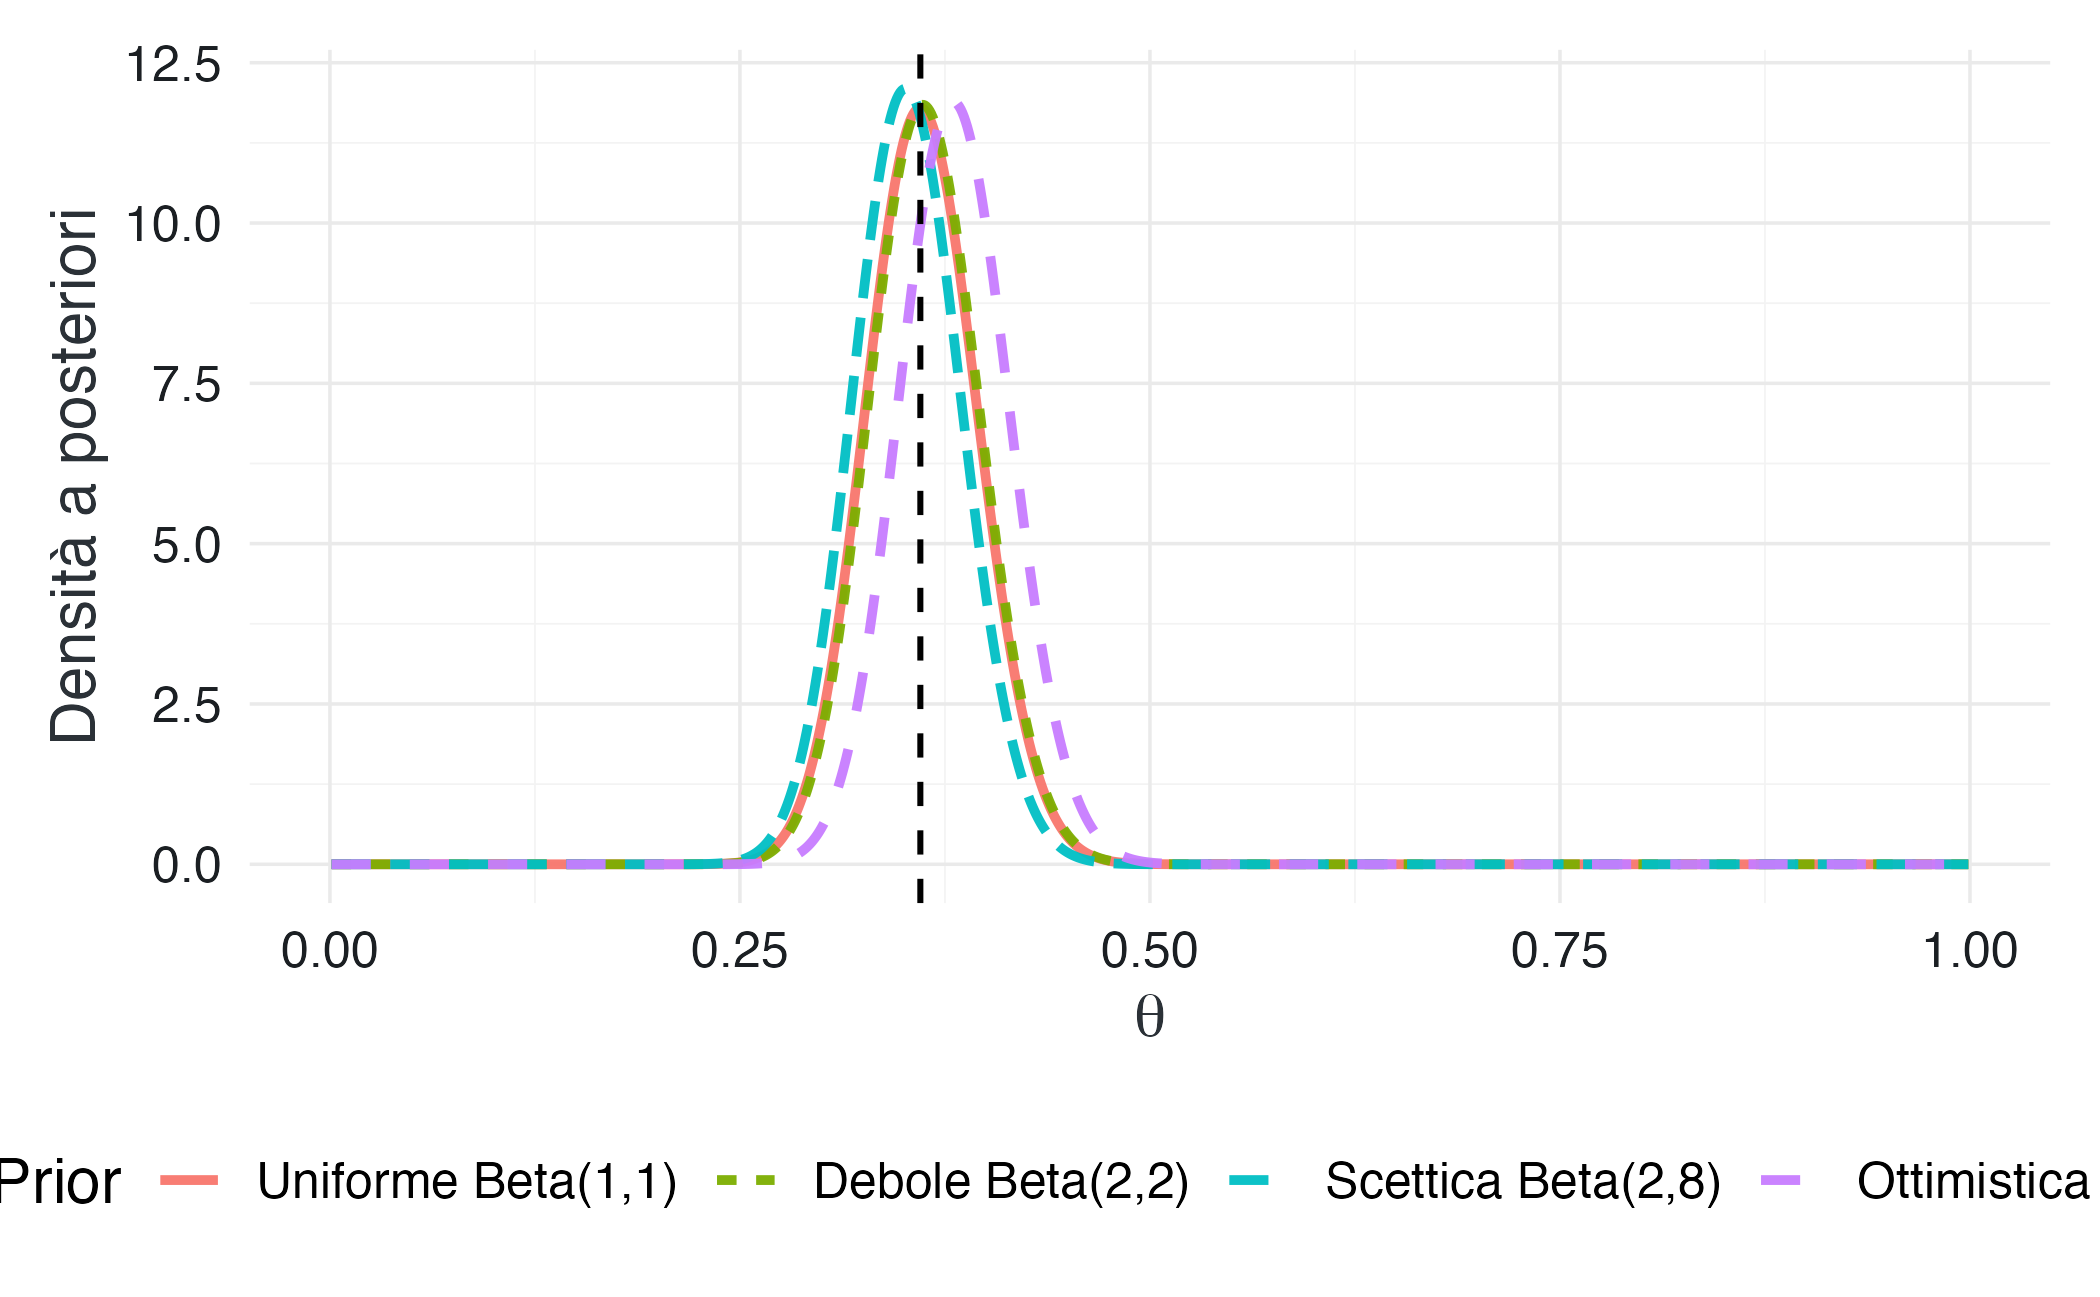
\includegraphics[width=0.85\linewidth,height=\textheight,keepaspectratio]{chapters/probability/15_aggiornamento_bayesiano_files/figure-pdf/fig-sensitivity-priors-1.png}

}

\caption{\label{fig-sensitivity-priors}Analisi di sensibilità: posterior
ottenute con prior diverse ma ragionevoli. Le conclusioni sono robuste
se le posterior risultano simili rispetto alle domande sostantive.}

\end{figure}%

\begin{Shaded}
\begin{Highlighting}[]
\NormalTok{summary\_sensitivity }\OtherTok{\textless{}{-}} \FunctionTok{data.frame}\NormalTok{(}
  \AttributeTok{Prior =}\NormalTok{ priors}\SpecialCharTok{$}\NormalTok{nome,}
  \AttributeTok{Alpha\_post =}\NormalTok{ priors}\SpecialCharTok{$}\NormalTok{alpha }\SpecialCharTok{+}\NormalTok{ y,}
  \AttributeTok{Beta\_post =}\NormalTok{ priors}\SpecialCharTok{$}\NormalTok{beta }\SpecialCharTok{+}\NormalTok{ n }\SpecialCharTok{{-}}\NormalTok{ y}
\NormalTok{)}

\NormalTok{summary\_sensitivity}\SpecialCharTok{$}\NormalTok{Media\_post }\OtherTok{\textless{}{-}} \FunctionTok{with}\NormalTok{(}
\NormalTok{  summary\_sensitivity,}
\NormalTok{  Alpha\_post }\SpecialCharTok{/}\NormalTok{ (Alpha\_post }\SpecialCharTok{+}\NormalTok{ Beta\_post)}
\NormalTok{)}
\NormalTok{summary\_sensitivity}\SpecialCharTok{$}\NormalTok{CI\_2}\FloatTok{.5} \OtherTok{\textless{}{-}} \FunctionTok{qbeta}\NormalTok{(}
  \FloatTok{0.025}\NormalTok{,}
\NormalTok{  summary\_sensitivity}\SpecialCharTok{$}\NormalTok{Alpha\_post,}
\NormalTok{  summary\_sensitivity}\SpecialCharTok{$}\NormalTok{Beta\_post}
\NormalTok{)}
\NormalTok{summary\_sensitivity}\SpecialCharTok{$}\NormalTok{CI\_97}\FloatTok{.5} \OtherTok{\textless{}{-}} \FunctionTok{qbeta}\NormalTok{(}
  \FloatTok{0.975}\NormalTok{,}
\NormalTok{  summary\_sensitivity}\SpecialCharTok{$}\NormalTok{Alpha\_post,}
\NormalTok{  summary\_sensitivity}\SpecialCharTok{$}\NormalTok{Beta\_post}
\NormalTok{)}
\NormalTok{summary\_sensitivity}\SpecialCharTok{$}\NormalTok{P\_theta\_gt\_0}\FloatTok{.40} \OtherTok{\textless{}{-}} \DecValTok{1} \SpecialCharTok{{-}} \FunctionTok{pbeta}\NormalTok{(}
  \FloatTok{0.40}\NormalTok{,}
\NormalTok{  summary\_sensitivity}\SpecialCharTok{$}\NormalTok{Alpha\_post,}
\NormalTok{  summary\_sensitivity}\SpecialCharTok{$}\NormalTok{Beta\_post}
\NormalTok{)}

\FunctionTok{round}\NormalTok{(summary\_sensitivity[, }\FunctionTok{c}\NormalTok{(}\StringTok{"Media\_post"}\NormalTok{, }\StringTok{"CI\_2.5"}\NormalTok{, }\StringTok{"CI\_97.5"}\NormalTok{, }\StringTok{"P\_theta\_gt\_0.40"}\NormalTok{)], }\DecValTok{3}\NormalTok{)}
\CommentTok{\#\textgreater{}   Media\_post CI\_2.5 CI\_97.5 P\_theta\_gt\_0.40}
\CommentTok{\#\textgreater{} 1      0.361  0.297   0.429           0.127}
\CommentTok{\#\textgreater{} 2      0.363  0.298   0.430           0.135}
\CommentTok{\#\textgreater{} 3      0.352  0.289   0.418           0.076}
\CommentTok{\#\textgreater{} 4      0.381  0.317   0.447           0.282}
\end{Highlighting}
\end{Shaded}

\subsection{Come leggere l'analisi di
sensibilità}\label{come-leggere-lanalisi-di-sensibilituxe0}

Se prior ragionevoli producono conclusioni molto diverse, i dati non
sono sufficienti a risolvere la questione e l'inferenza dipende in modo
rilevante dalle assunzioni iniziali. Ciò non è necessariamente un
problema, ma è un'informazione importante da comunicare.

Se invece prior ragionevoli producono posterior simili rispetto alla
domanda sostantiva, possiamo dire che le conclusioni sono relativamente
robuste.

\begin{tcolorbox}[enhanced jigsaw, arc=.35mm, bottomrule=.15mm, bottomtitle=1mm, breakable, colback=white, colbacktitle=quarto-callout-note-color!10!white, colframe=quarto-callout-note-color-frame, coltitle=black, left=2mm, leftrule=.75mm, opacityback=0, opacitybacktitle=0.6, rightrule=.15mm, title=\textcolor{quarto-callout-note-color}{\faInfo}\hspace{0.5em}{Nota}, titlerule=0mm, toprule=.15mm, toptitle=1mm]

L'analisi di sensibilità non serve a nascondere la prior. Al contrario,
serve a renderne visibile il ruolo.

\end{tcolorbox}

\section{Il caso Normale-Normale: aggiornare una
media}\label{sec-normal-normal-update}

Il caso Beta-Binomiale è utile per le proporzioni. Un secondo caso
fondamentale riguarda la stima di una media.

Supponiamo di voler stimare il punteggio medio \(\mu\) di una scala
psicologica. Supponiamo che le osservazioni siano approssimativamente
normali con varianza nota \(\sigma^2\):

\[
X_i \mid \mu \sim \mathcal{N}(\mu, \sigma^2).
\]

Poniamo una prior normale sulla media:

\[
\mu \sim \mathcal{N}(\mu_0, \sigma_0^2).
\]

In questo caso, la posterior è ancora normale:

\[
\mu \mid x \sim \mathcal{N}(\mu_{\text{post}}, \sigma^2_{\text{post}}).
\]

\subsection{La media posterior come media
pesata}\label{la-media-posterior-come-media-pesata}

Definiamo le precisioni:

\[
\tau_0 = \frac{1}{\sigma_0^2},
\qquad
\tau_{\text{dati}} = \frac{n}{\sigma^2}.
\]

La media a posteriori è:

\[
\mu_{\text{post}} =
\frac{\tau_0\mu_0 + \tau_{\text{dati}}\bar{x}}
{\tau_0 + \tau_{\text{dati}}}.
\]

La precisione a posteriori è:

\[
\tau_{\text{post}} = \tau_0 + \tau_{\text{dati}}.
\]

Quindi:

\[
\sigma^2_{\text{post}} = \frac{1}{\tau_{\text{post}}}.
\]

\begin{tcolorbox}[enhanced jigsaw, arc=.35mm, bottomrule=.15mm, bottomtitle=1mm, breakable, colback=white, colbacktitle=quarto-callout-important-color!10!white, colframe=quarto-callout-important-color-frame, coltitle=black, left=2mm, leftrule=.75mm, opacityback=0, opacitybacktitle=0.6, rightrule=.15mm, title=\textcolor{quarto-callout-important-color}{\faExclamation}\hspace{0.5em}{Importante}, titlerule=0mm, toprule=.15mm, toptitle=1mm]

Nel caso Normale-Normale, l'aggiornamento bayesiano è una media
ponderata tra il prior e i dati. I pesi sono le precisioni: la fonte più
precisa pesa di più.

\end{tcolorbox}

\subsection{Esempio numerico}\label{esempio-numerico-2}

Uno psicologo ha una credenza iniziale secondo cui il punteggio medio di
una scala di ansia sia circa 50, con una deviazione standard a priori
pari a 10:

\[
\mu \sim \mathcal{N}(50, 10^2).
\]

Successivamente, raccoglie dati da \(n=30\) studenti. La media osservata
è \(\bar{x}=56\) e la deviazione standard nota o assunta è
\(\sigma=15\).

\begin{Shaded}
\begin{Highlighting}[]
\NormalTok{mu0 }\OtherTok{\textless{}{-}} \DecValTok{50}
\NormalTok{sigma0 }\OtherTok{\textless{}{-}} \DecValTok{10}
\NormalTok{n\_norm }\OtherTok{\textless{}{-}} \DecValTok{30}
\NormalTok{xbar }\OtherTok{\textless{}{-}} \DecValTok{56}
\NormalTok{sigma }\OtherTok{\textless{}{-}} \DecValTok{15}

\NormalTok{tau0 }\OtherTok{\textless{}{-}} \DecValTok{1} \SpecialCharTok{/}\NormalTok{ sigma0}\SpecialCharTok{\^{}}\DecValTok{2}
\NormalTok{tau\_data }\OtherTok{\textless{}{-}}\NormalTok{ n\_norm }\SpecialCharTok{/}\NormalTok{ sigma}\SpecialCharTok{\^{}}\DecValTok{2}
\NormalTok{tau\_post }\OtherTok{\textless{}{-}}\NormalTok{ tau0 }\SpecialCharTok{+}\NormalTok{ tau\_data}
\NormalTok{sigma\_post }\OtherTok{\textless{}{-}} \FunctionTok{sqrt}\NormalTok{(}\DecValTok{1} \SpecialCharTok{/}\NormalTok{ tau\_post)}
\NormalTok{mu\_post }\OtherTok{\textless{}{-}}\NormalTok{ (tau0 }\SpecialCharTok{*}\NormalTok{ mu0 }\SpecialCharTok{+}\NormalTok{ tau\_data }\SpecialCharTok{*}\NormalTok{ xbar) }\SpecialCharTok{/}\NormalTok{ tau\_post}

\NormalTok{theta\_grid\_norm }\OtherTok{\textless{}{-}} \FunctionTok{seq}\NormalTok{(}\DecValTok{25}\NormalTok{, }\DecValTok{80}\NormalTok{, }\AttributeTok{length.out =} \DecValTok{1000}\NormalTok{)}
\NormalTok{prior\_norm }\OtherTok{\textless{}{-}} \FunctionTok{dnorm}\NormalTok{(theta\_grid\_norm, mu0, sigma0)}
\NormalTok{lik\_norm }\OtherTok{\textless{}{-}} \FunctionTok{dnorm}\NormalTok{(theta\_grid\_norm, xbar, sigma }\SpecialCharTok{/} \FunctionTok{sqrt}\NormalTok{(n\_norm))}
\NormalTok{post\_norm }\OtherTok{\textless{}{-}} \FunctionTok{dnorm}\NormalTok{(theta\_grid\_norm, mu\_post, sigma\_post)}

\NormalTok{lik\_norm\_scaled }\OtherTok{\textless{}{-}}\NormalTok{ lik\_norm }\SpecialCharTok{*} \FunctionTok{max}\NormalTok{(prior\_norm) }\SpecialCharTok{/} \FunctionTok{max}\NormalTok{(lik\_norm)}

\NormalTok{normal\_plot\_data }\OtherTok{\textless{}{-}} \FunctionTok{data.frame}\NormalTok{(}
  \AttributeTok{mu =} \FunctionTok{rep}\NormalTok{(theta\_grid\_norm, }\DecValTok{3}\NormalTok{),}
  \AttributeTok{density =} \FunctionTok{c}\NormalTok{(prior\_norm, lik\_norm\_scaled, post\_norm),}
  \AttributeTok{componente =} \FunctionTok{factor}\NormalTok{(}
    \FunctionTok{rep}\NormalTok{(}\FunctionTok{c}\NormalTok{(}\StringTok{"Prior"}\NormalTok{, }\StringTok{"Verosimiglianza (riscalata)"}\NormalTok{, }\StringTok{"Posterior"}\NormalTok{),}
        \AttributeTok{each =} \FunctionTok{length}\NormalTok{(theta\_grid\_norm)),}
    \AttributeTok{levels =} \FunctionTok{c}\NormalTok{(}\StringTok{"Prior"}\NormalTok{, }\StringTok{"Verosimiglianza (riscalata)"}\NormalTok{, }\StringTok{"Posterior"}\NormalTok{)}
\NormalTok{  )}
\NormalTok{)}

\FunctionTok{ggplot}\NormalTok{(normal\_plot\_data, }\FunctionTok{aes}\NormalTok{(}\AttributeTok{x =}\NormalTok{ mu, }\AttributeTok{y =}\NormalTok{ density,}
                             \AttributeTok{color =}\NormalTok{ componente, }\AttributeTok{linetype =}\NormalTok{ componente)) }\SpecialCharTok{+}
  \FunctionTok{geom\_line}\NormalTok{(}\AttributeTok{linewidth =} \FloatTok{1.1}\NormalTok{) }\SpecialCharTok{+}
  \FunctionTok{labs}\NormalTok{(}
    \AttributeTok{x =} \FunctionTok{expression}\NormalTok{(mu),}
    \AttributeTok{y =} \StringTok{"Densità / scala relativa"}\NormalTok{,}
    \AttributeTok{color =} \StringTok{""}\NormalTok{,}
    \AttributeTok{linetype =} \StringTok{""}
\NormalTok{  ) }\SpecialCharTok{+}
  \FunctionTok{theme}\NormalTok{(}\AttributeTok{legend.position =} \StringTok{"bottom"}\NormalTok{)}
\end{Highlighting}
\end{Shaded}

\begin{figure}[H]

\centering{

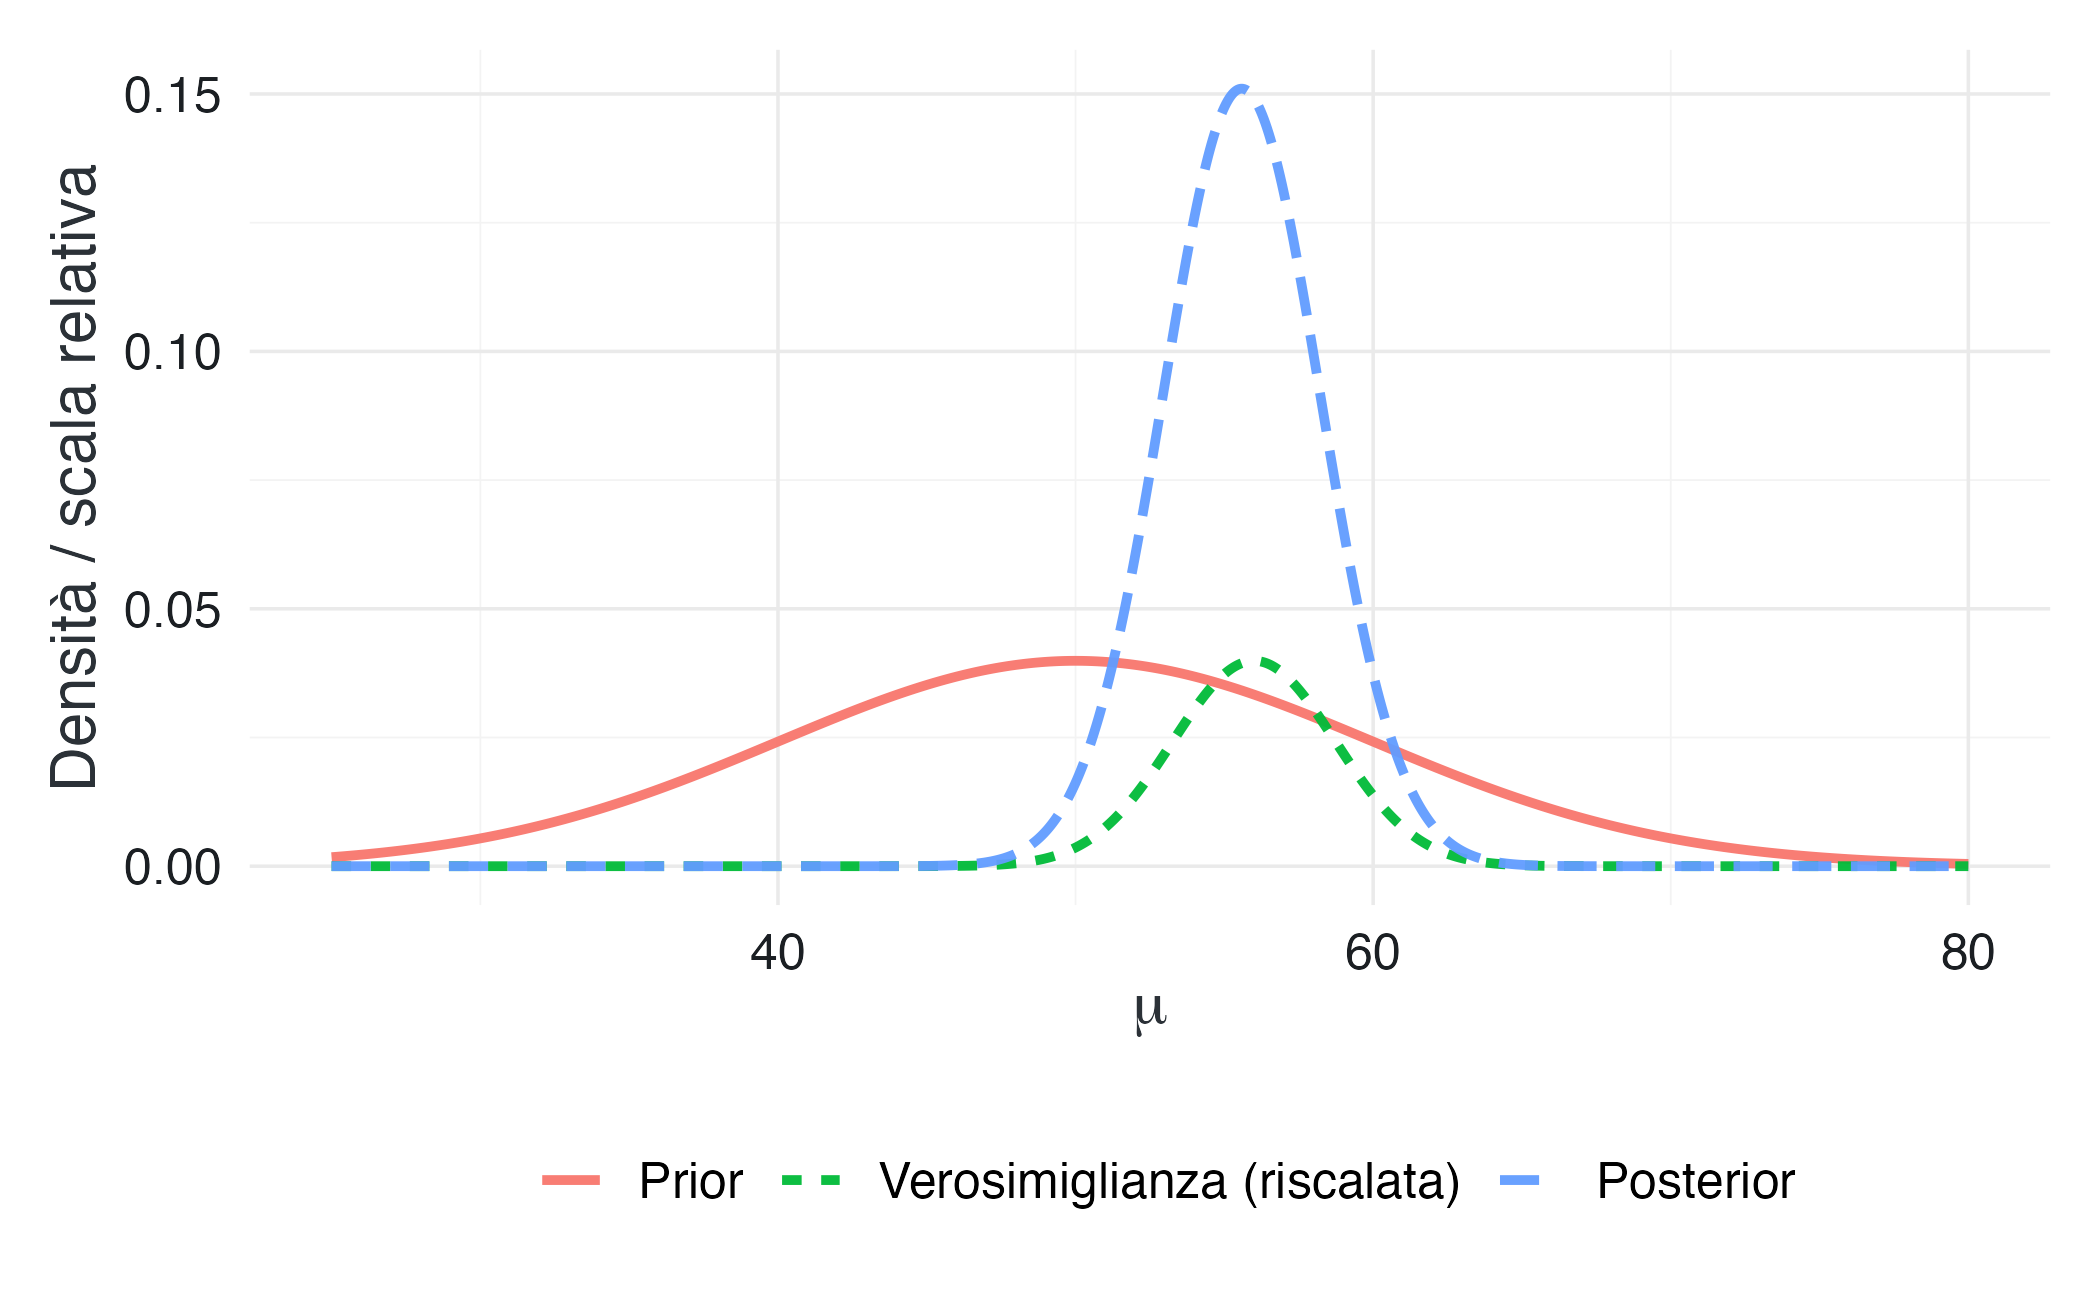
\includegraphics[width=0.85\linewidth,height=\textheight,keepaspectratio]{chapters/probability/15_aggiornamento_bayesiano_files/figure-pdf/fig-normal-normal-update-1.png}

}

\caption{\label{fig-normal-normal-update}Aggiornamento Normale-Normale:
la posterior è una media pesata tra prior e verosimiglianza, con pesi
proporzionali alle precisioni.}

\end{figure}%

\begin{Shaded}
\begin{Highlighting}[]
\FunctionTok{cat}\NormalTok{(}\StringTok{"Media prior:"}\NormalTok{, mu0, }\StringTok{"}\SpecialCharTok{\textbackslash{}n}\StringTok{"}\NormalTok{)}
\CommentTok{\#\textgreater{} Media prior: 50}
\FunctionTok{cat}\NormalTok{(}\StringTok{"Media dati:"}\NormalTok{, xbar, }\StringTok{"}\SpecialCharTok{\textbackslash{}n}\StringTok{"}\NormalTok{)}
\CommentTok{\#\textgreater{} Media dati: 56}
\FunctionTok{cat}\NormalTok{(}\StringTok{"Media posterior:"}\NormalTok{, }\FunctionTok{round}\NormalTok{(mu\_post, }\DecValTok{2}\NormalTok{), }\StringTok{"}\SpecialCharTok{\textbackslash{}n}\StringTok{"}\NormalTok{)}
\CommentTok{\#\textgreater{} Media posterior: 55.6}
\FunctionTok{cat}\NormalTok{(}\StringTok{"Deviazione standard posterior:"}\NormalTok{, }\FunctionTok{round}\NormalTok{(sigma\_post, }\DecValTok{2}\NormalTok{), }\StringTok{"}\SpecialCharTok{\textbackslash{}n}\StringTok{"}\NormalTok{)}
\CommentTok{\#\textgreater{} Deviazione standard posterior: 2.64}
\FunctionTok{cat}\NormalTok{(}\StringTok{"Precisione prior:"}\NormalTok{, }\FunctionTok{round}\NormalTok{(tau0, }\DecValTok{4}\NormalTok{), }\StringTok{"}\SpecialCharTok{\textbackslash{}n}\StringTok{"}\NormalTok{)}
\CommentTok{\#\textgreater{} Precisione prior: 0.01}
\FunctionTok{cat}\NormalTok{(}\StringTok{"Precisione dati:"}\NormalTok{, }\FunctionTok{round}\NormalTok{(tau\_data, }\DecValTok{4}\NormalTok{), }\StringTok{"}\SpecialCharTok{\textbackslash{}n}\StringTok{"}\NormalTok{)}
\CommentTok{\#\textgreater{} Precisione dati: 0.133}
\FunctionTok{cat}\NormalTok{(}\StringTok{"Precisione posterior:"}\NormalTok{, }\FunctionTok{round}\NormalTok{(tau\_post, }\DecValTok{4}\NormalTok{), }\StringTok{"}\SpecialCharTok{\textbackslash{}n}\StringTok{"}\NormalTok{)}
\CommentTok{\#\textgreater{} Precisione posterior: 0.143}
\end{Highlighting}
\end{Shaded}

\subsection{Interpretazione}\label{interpretazione-3}

La media a posteriori si colloca tra la media prior e la media
campionaria. Se la prior è molto incerta, la posterior si avvicina ai
dati. Se i dati sono pochi o rumorosi, la posterior rimane più vicina
alla prior.

Questo esempio illustra una proprietà generale dell'approccio bayesiano:
l'inferenza non sceglie tra la conoscenza precedente e i dati, ma li
combina in modo proporzionale alla loro informatività.

\section{Aggiornamento sequenziale}\label{sec-sequential-updating}

Uno dei vantaggi concettuali dell'inferenza bayesiana è che
l'aggiornamento può avvenire in modo sequenziale.

Supponiamo di osservare due insiemi di dati indipendenti, \(y_1\) e
\(y_2\). Dopo il primo studio otteniamo:

\[
p(\theta \mid y_1) \propto p(y_1 \mid \theta)p(\theta).
\]

Quando arriva il secondo studio, possiamo usare la posterior del primo
studio come prior per il secondo:

\[
p(\theta \mid y_1, y_2)
\propto p(y_2 \mid \theta)p(\theta \mid y_1).
\]

Sostituendo la prima equazione nella seconda, otteniamo:

\[
p(\theta \mid y_1, y_2)
\propto p(\theta)p(y_1 \mid \theta)p(y_2 \mid \theta).
\]

Quindi, se gli studi sono indipendenti condizionatamente al parametro,
aggiornare in sequenza o aggiornare tutto insieme porta allo stesso
risultato.

\subsection{Esempio Beta-Binomiale
sequenziale}\label{esempio-beta-binomiale-sequenziale}

Riprendiamo i dati complessivi \(y=72\) su \(n=200\), ma immaginiamo che
siano arrivati in due fasi:

\begin{itemize}
\tightlist
\item
  primo studio: \(y_1 = 18\) su \(n_1 = 50\);
\item
  secondo studio: \(y_2 = 54\) su \(n_2 = 150\).
\end{itemize}

\begin{Shaded}
\begin{Highlighting}[]
\NormalTok{alpha0 }\OtherTok{\textless{}{-}} \DecValTok{2}
\NormalTok{beta0 }\OtherTok{\textless{}{-}} \DecValTok{2}

\NormalTok{n1 }\OtherTok{\textless{}{-}} \DecValTok{50}
\NormalTok{y1 }\OtherTok{\textless{}{-}} \DecValTok{18}
\NormalTok{n2 }\OtherTok{\textless{}{-}} \DecValTok{150}
\NormalTok{y2 }\OtherTok{\textless{}{-}} \DecValTok{54}

\CommentTok{\# Aggiornamento sequenziale}
\NormalTok{alpha\_after\_1 }\OtherTok{\textless{}{-}}\NormalTok{ alpha0 }\SpecialCharTok{+}\NormalTok{ y1}
\NormalTok{beta\_after\_1 }\OtherTok{\textless{}{-}}\NormalTok{ beta0 }\SpecialCharTok{+}\NormalTok{ n1 }\SpecialCharTok{{-}}\NormalTok{ y1}

\NormalTok{alpha\_after\_2 }\OtherTok{\textless{}{-}}\NormalTok{ alpha\_after\_1 }\SpecialCharTok{+}\NormalTok{ y2}
\NormalTok{beta\_after\_2 }\OtherTok{\textless{}{-}}\NormalTok{ beta\_after\_1 }\SpecialCharTok{+}\NormalTok{ n2 }\SpecialCharTok{{-}}\NormalTok{ y2}

\CommentTok{\# Aggiornamento in un solo passo}
\NormalTok{alpha\_batch }\OtherTok{\textless{}{-}}\NormalTok{ alpha0 }\SpecialCharTok{+}\NormalTok{ y1 }\SpecialCharTok{+}\NormalTok{ y2}
\NormalTok{beta\_batch }\OtherTok{\textless{}{-}}\NormalTok{ beta0 }\SpecialCharTok{+}\NormalTok{ (n1 }\SpecialCharTok{+}\NormalTok{ n2) }\SpecialCharTok{{-}}\NormalTok{ (y1 }\SpecialCharTok{+}\NormalTok{ y2)}

\FunctionTok{cat}\NormalTok{(}\StringTok{"Posterior sequenziale: Beta("}\NormalTok{, alpha\_after\_2, }\StringTok{", "}\NormalTok{, beta\_after\_2, }\StringTok{")}\SpecialCharTok{\textbackslash{}n}\StringTok{"}\NormalTok{, }\AttributeTok{sep =} \StringTok{""}\NormalTok{)}
\CommentTok{\#\textgreater{} Posterior sequenziale: Beta(74, 130)}
\FunctionTok{cat}\NormalTok{(}\StringTok{"Posterior in un solo passo: Beta("}\NormalTok{, alpha\_batch, }\StringTok{", "}\NormalTok{, beta\_batch, }\StringTok{")}\SpecialCharTok{\textbackslash{}n}\StringTok{"}\NormalTok{, }\AttributeTok{sep =} \StringTok{""}\NormalTok{)}
\CommentTok{\#\textgreater{} Posterior in un solo passo: Beta(74, 130)}
\end{Highlighting}
\end{Shaded}

\begin{Shaded}
\begin{Highlighting}[]
\NormalTok{seq\_plot\_data }\OtherTok{\textless{}{-}} \FunctionTok{data.frame}\NormalTok{(}
  \AttributeTok{theta =} \FunctionTok{rep}\NormalTok{(theta\_grid, }\DecValTok{4}\NormalTok{),}
  \AttributeTok{density =} \FunctionTok{c}\NormalTok{(}
    \FunctionTok{dbeta}\NormalTok{(theta\_grid, alpha0, beta0),}
    \FunctionTok{dbeta}\NormalTok{(theta\_grid, alpha\_after\_1, beta\_after\_1),}
    \FunctionTok{dbeta}\NormalTok{(theta\_grid, alpha\_after\_2, beta\_after\_2),}
    \FunctionTok{dbeta}\NormalTok{(theta\_grid, alpha\_batch, beta\_batch)}
\NormalTok{  ),}
  \AttributeTok{fase =} \FunctionTok{factor}\NormalTok{(}
    \FunctionTok{rep}\NormalTok{(}\FunctionTok{c}\NormalTok{(}\StringTok{"Prior iniziale"}\NormalTok{,}
          \StringTok{"Posterior dopo studio 1"}\NormalTok{,}
          \StringTok{"Posterior sequenziale finale"}\NormalTok{,}
          \StringTok{"Posterior con tutti i dati"}\NormalTok{),}
        \AttributeTok{each =} \FunctionTok{length}\NormalTok{(theta\_grid)),}
    \AttributeTok{levels =} \FunctionTok{c}\NormalTok{(}\StringTok{"Prior iniziale"}\NormalTok{,}
               \StringTok{"Posterior dopo studio 1"}\NormalTok{,}
               \StringTok{"Posterior sequenziale finale"}\NormalTok{,}
               \StringTok{"Posterior con tutti i dati"}\NormalTok{)}
\NormalTok{  )}
\NormalTok{)}

\FunctionTok{ggplot}\NormalTok{(seq\_plot\_data, }\FunctionTok{aes}\NormalTok{(}\AttributeTok{x =}\NormalTok{ theta, }\AttributeTok{y =}\NormalTok{ density,}
                          \AttributeTok{color =}\NormalTok{ fase, }\AttributeTok{linetype =}\NormalTok{ fase)) }\SpecialCharTok{+}
  \FunctionTok{geom\_line}\NormalTok{(}\AttributeTok{linewidth =} \FloatTok{1.1}\NormalTok{) }\SpecialCharTok{+}
  \FunctionTok{labs}\NormalTok{(}
    \AttributeTok{x =} \FunctionTok{expression}\NormalTok{(theta),}
    \AttributeTok{y =} \StringTok{"Densità"}\NormalTok{,}
    \AttributeTok{color =} \StringTok{""}\NormalTok{,}
    \AttributeTok{linetype =} \StringTok{""}
\NormalTok{  ) }\SpecialCharTok{+}
  \FunctionTok{theme}\NormalTok{(}\AttributeTok{legend.position =} \StringTok{"bottom"}\NormalTok{)}
\end{Highlighting}
\end{Shaded}

\begin{figure}[H]

\centering{

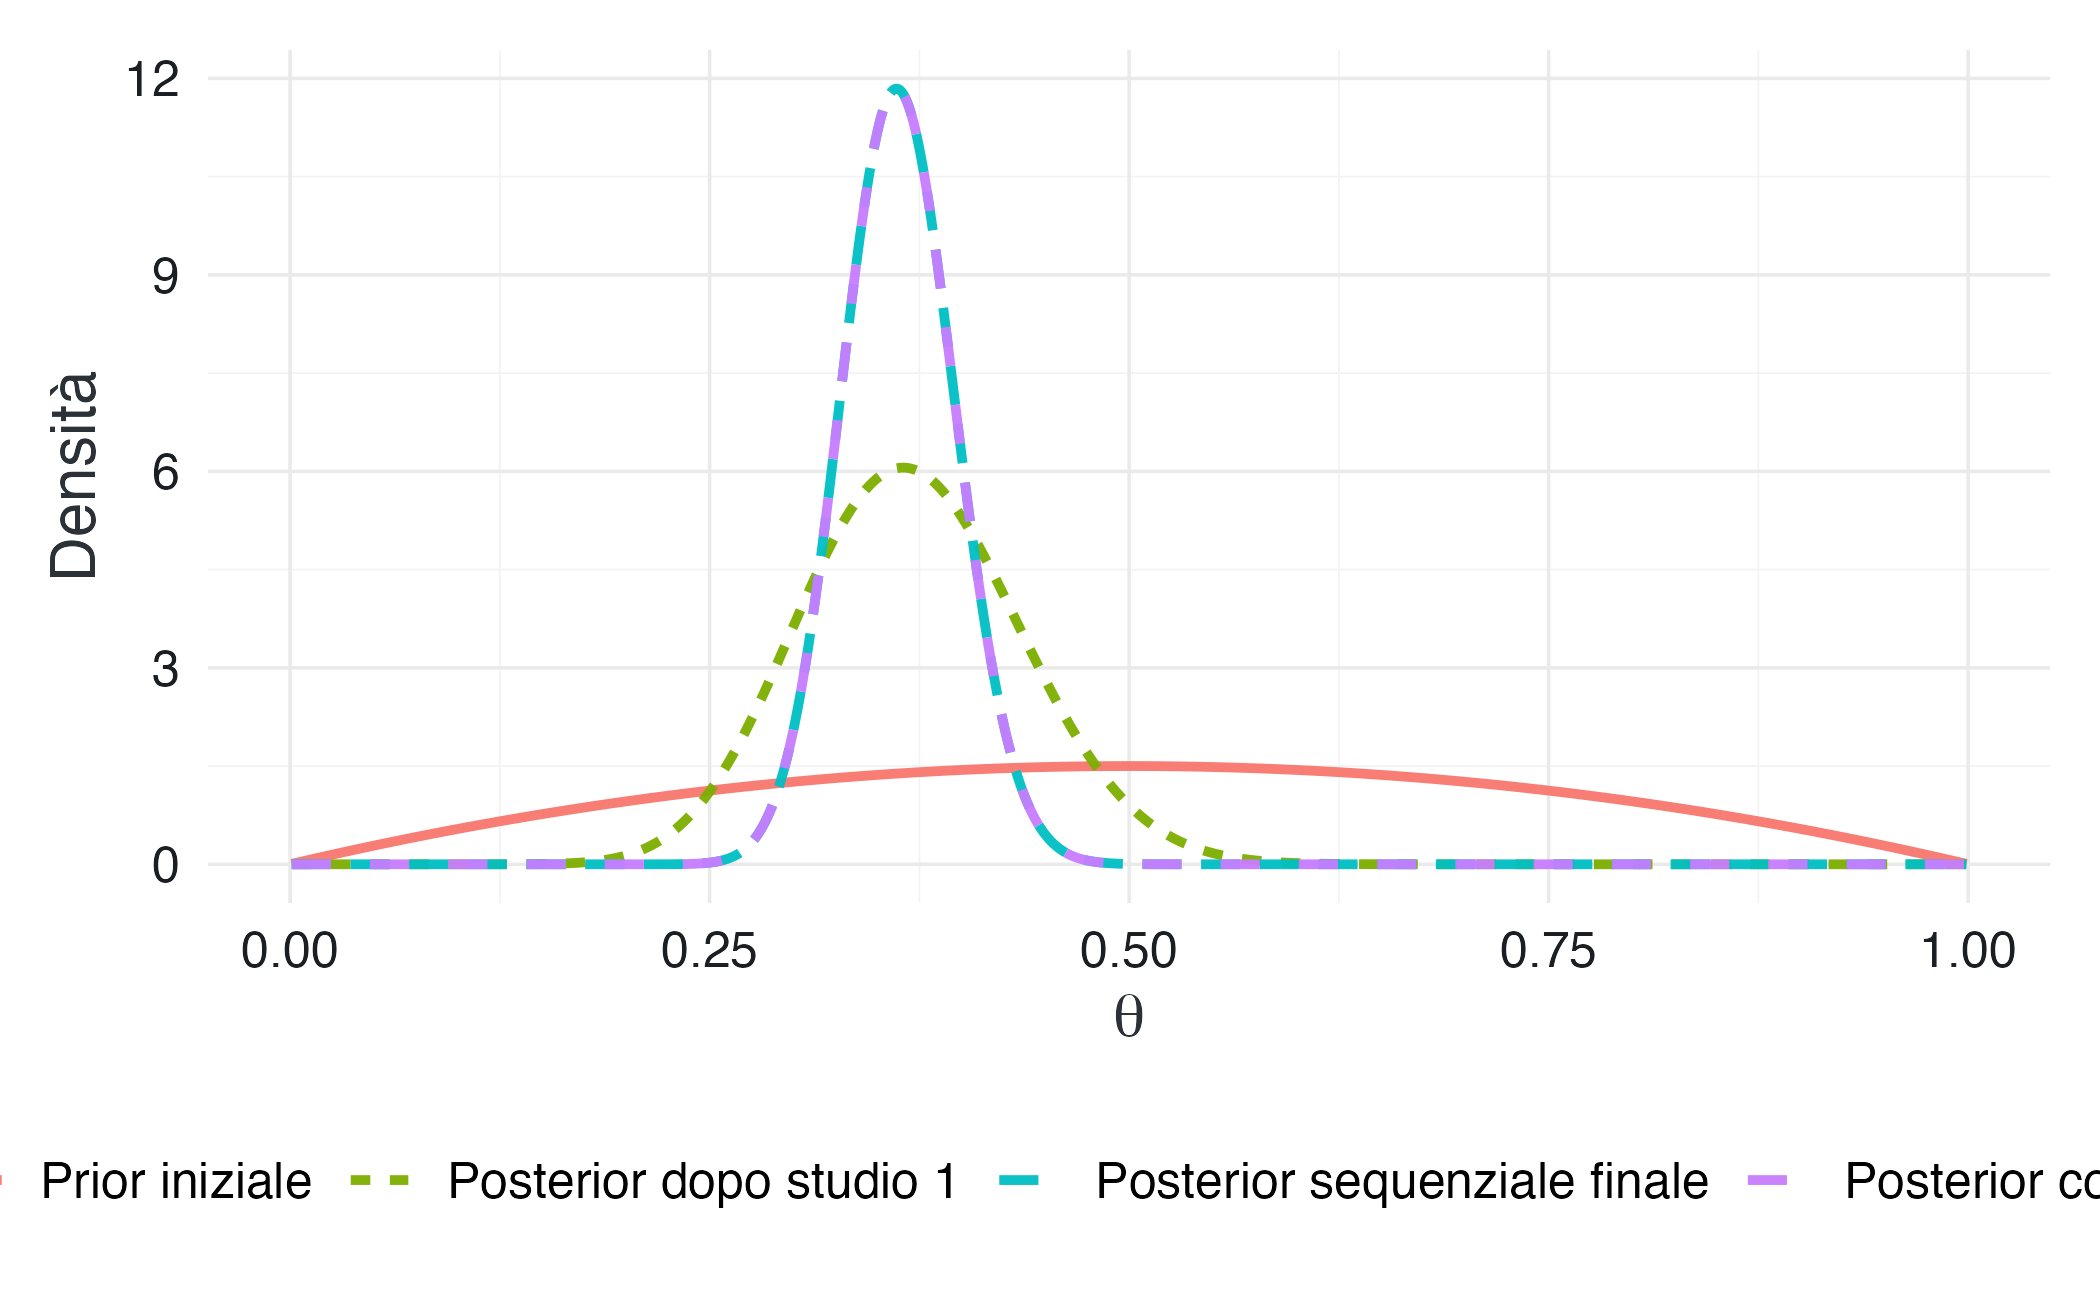
\includegraphics[width=0.85\linewidth,height=\textheight,keepaspectratio]{chapters/probability/15_aggiornamento_bayesiano_files/figure-pdf/fig-sequential-updating-1.png}

}

\caption{\label{fig-sequential-updating}Aggiornamento sequenziale: la
posterior dopo il primo studio diventa la prior per il secondo.
L'aggiornamento finale coincide con quello ottenuto usando tutti i dati
insieme.}

\end{figure}%

La posterior sequenziale finale e la posterior ottenuta utilizzando
tutti i dati insieme coincidono. Questo risultato esprime la
\textbf{coerenza temporale} dell'aggiornamento bayesiano: ciò che
impariamo oggi può diventare la base razionale per imparare domani.

\begin{tcolorbox}[enhanced jigsaw, arc=.35mm, bottomrule=.15mm, bottomtitle=1mm, breakable, colback=white, colbacktitle=quarto-callout-note-color!10!white, colframe=quarto-callout-note-color-frame, coltitle=black, left=2mm, leftrule=.75mm, opacityback=0, opacitybacktitle=0.6, rightrule=.15mm, title=\textcolor{quarto-callout-note-color}{\faInfo}\hspace{0.5em}{Collegamento con la combinazione di evidenze}, titlerule=0mm, toprule=.15mm, toptitle=1mm]

Nel Capitolo~\ref{sec-prob-inference-uncertainty} abbiamo discusso
l'idea che le evidenze indipendenti possano essere combinate. Qui, la
stessa idea si presenta nella sua forma più propriamente bayesiana: le
verosimiglianze degli studi indipendenti si moltiplicano e la posterior
risultante riassume tutte le informazioni disponibili.

\end{tcolorbox}

\section{Cosa la posterior può e non può
dirci}\label{sec-what-posterior-can-say}

La posterior è uno strumento potente per rappresentare l'incertezza
epistemica. Permette di rispondere direttamente a domande come:

\begin{itemize}
\tightlist
\item
  Qual è il valore più plausibile del parametro dopo aver osservato i
  dati?
\item
  Quali valori restano credibili?
\item
  Qual è la probabilità che il parametro superi una soglia clinicamente
  rilevante?
\item
  Quanto cambiano le conclusioni se si usa una prior diversa?
\end{itemize}

Tuttavia, la posterior non elimina i limiti del modello e dei dati.

\subsection{Condizionamento sul
modello}\label{condizionamento-sul-modello}

La posterior è sempre condizionata a un modello:

\[
p(\theta \mid y, M).
\]

Ciò significa che le probabilità posteriori sono valide \textbf{solo se
si considera il modello adottato}. Se il modello è inadeguato, anche la
posterior può risultare fuorviante.

\subsection{Qualità dei dati}\label{qualituxe0-dei-dati}

L'aggiornamento bayesiano non corregge automaticamente dati distorti. Se
il campione è selezionato in modo errato, se lo strumento misura il
costrutto sbagliato o se le risposte sono sistematicamente alterate
dalla desiderabilità sociale, la posteriori può diventare molto precisa
attorno a un valore errato.

Questo punto è stato discusso nel
Capitolo~\ref{sec-prob-inference-uncertainty}. Lo richiamiamo qui perché
è una condizione essenziale dell'interpretazione bayesiana:

\begin{quote}
la posterior quantifica l'incertezza \textbf{condizionatamente} ai dati,
al modello e alla prior, ma non garantisce da sola la validità
scientifica dello studio.
\end{quote}

\subsection{Prior inappropriate}\label{prior-inappropriate}

Una prior estremamente forte e incompatibile con il fenomeno può
dominare l'inferenza, soprattutto quando i dati a disposizione sono
pochi. Per questo motivo è importante:

\begin{itemize}
\tightlist
\item
  dichiarare la prior;
\item
  motivarla sostantivamente;
\item
  valutarne l'impatto tramite un'analisi di sensibilità.
\end{itemize}

\begin{tcolorbox}[enhanced jigsaw, arc=.35mm, bottomrule=.15mm, bottomtitle=1mm, breakable, colback=white, colbacktitle=quarto-callout-warning-color!10!white, colframe=quarto-callout-warning-color-frame, coltitle=black, left=2mm, leftrule=.75mm, opacityback=0, opacitybacktitle=0.6, rightrule=.15mm, title=\textcolor{quarto-callout-warning-color}{\faExclamationTriangle}\hspace{0.5em}{Una posterior precisa non basta}, titlerule=0mm, toprule=.15mm, toptitle=1mm]

Una posterior stretta indica una bassa incertezza condizionata al
modello. Tuttavia, non dimostra che il modello sia corretto, che il
campione sia rappresentativo o che la misura sia valida.

\end{tcolorbox}

\section{Cosa lasciamo ai capitoli
successivi}\label{sec-advanced-topics-not-here}

Alcuni argomenti sono importanti, ma non sono necessari per il primo
incontro con l'aggiornamento bayesiano. Per mantenere il capitolo
introduttivo e coerente, non li sviluppiamo qui:

\begin{itemize}
\tightlist
\item
  la score function e l'informazione di Fisher;
\item
  l'approssimazione di Laplace;
\item
  il teorema di Bernstein-von Mises;
\item
  i metodi computazionali come MCMC, HMC e inferenza variazionale;
\item
  la comparazione di modelli tramite evidenza marginale o fattori di
  Bayes.
\end{itemize}

Questi temi saranno ripresi in seguito, quando il lettore avrà acquisito
una comprensione operativa di prior, verosimiglianza e posterior.

\section*{Riflessioni conclusive}\label{riflessioni-conclusive-14}

\markright{Riflessioni conclusive}

Questo capitolo completa il passaggio dalla verosimiglianza
all'inferenza bayesiana vera e propria.

La verosimiglianza riassume ciò che i dati dicono sui possibili valori
del parametro. La prior riassume ciò che era plausibile prima di
osservare quei dati. La posterior combina queste due fonti di
informazione in una nuova distribuzione di probabilità.

Nel caso Beta-Binomiale, l'aggiornamento è particolarmente trasparente:
i successi e gli insuccessi osservati modificano direttamente i
parametri della distribuzione Beta. Nel caso Normale-Normale, la
posterior è una media pesata tra prior e dati, con pesi proporzionali
alle rispettive precisioni. Nel caso di aggiornamento sequenziale, la
posterior ottenuta dopo la prima osservazione diventa la prior per la
successiva.

Il messaggio concettuale è unico:

\begin{quote}
l'inferenza bayesiana è una procedura coerente per aggiornare le
credenze alla luce dell'evidenza.
\end{quote}

Tale coerenza non esime però il ricercatore dalla responsabilità
scientifica. La posterior deve sempre essere interpretata alla luce del
modello, della prior, della qualità dei dati e del disegno della
ricerca.

\section*{Punti chiave da ricordare}\label{punti-chiave-da-ricordare-14}
\addcontentsline{toc}{section}{Punti chiave da ricordare}

\markright{Punti chiave da ricordare}

\begin{tcolorbox}[enhanced jigsaw, arc=.35mm, bottomrule=.15mm, bottomtitle=1mm, breakable, colback=white, colbacktitle=quarto-callout-important-color!10!white, colframe=quarto-callout-important-color-frame, coltitle=black, left=2mm, leftrule=.75mm, opacityback=0, opacitybacktitle=0.6, rightrule=.15mm, title=\textcolor{quarto-callout-important-color}{\faExclamation}\hspace{0.5em}{Importante}, titlerule=0mm, toprule=.15mm, toptitle=1mm]

\begin{enumerate}
\def\labelenumi{\arabic{enumi}.}
\item
  \textbf{Regola di Bayes}

  \[
  p(\theta \mid y) =
  \frac{p(y \mid \theta)p(\theta)}{p(y)}.
  \]
\item
  \textbf{Forma proporzionale}

  \[
  p(\theta \mid y) \propto p(y \mid \theta)p(\theta).
  \]
\item
  \textbf{Beta-Binomiale}

  Se

  \[
  \theta \sim \text{Beta}(\alpha,\beta),
  \qquad
  Y \mid \theta \sim \text{Binomiale}(n,\theta),
  \]

  allora

  \[
  \theta \mid Y=y \sim
  \text{Beta}(\alpha+y,\beta+n-y).
  \]
\item
  \textbf{Normale-Normale}

  La media posterior è una media pesata:

  \[
  \mu_{\text{post}} =
  \frac{\tau_0\mu_0 + \tau_{\text{dati}}\bar{x}}
  {\tau_0 + \tau_{\text{dati}}}.
  \]

  La precisione posterior è la somma delle precisioni:

  \[
  \tau_{\text{post}} = \tau_0 + \tau_{\text{dati}}.
  \]
\item
  \textbf{Aggiornamento sequenziale}

  \[
  p(\theta \mid y_1,y_2)
  \propto
  p(y_2 \mid \theta)p(\theta \mid y_1).
  \]
\item
  \textbf{Analisi di sensibilità}

  Confrontare posterior ottenute con prior diverse aiuta a capire se le
  conclusioni dipendono fortemente dalle assunzioni iniziali.
\item
  \textbf{Interpretazione condizionata}

  La posterior quantifica l'incertezza dato il modello, la prior e i
  dati. Non corregge automaticamente bias, errori di misura o modelli
  inadeguati.
\end{enumerate}

\end{tcolorbox}

\begin{tcolorbox}[enhanced jigsaw, arc=.35mm, bottomrule=.15mm, bottomtitle=1mm, breakable, colback=white, colbacktitle=quarto-callout-important-color!10!white, colframe=quarto-callout-important-color-frame, coltitle=black, left=2mm, leftrule=.75mm, opacityback=0, opacitybacktitle=0.6, rightrule=.15mm, title=\textcolor{quarto-callout-important-color}{\faExclamation}\hspace{0.5em}{Esercizi}, titlerule=0mm, toprule=.15mm, toptitle=1mm]

\begin{enumerate}
\def\labelenumi{\arabic{enumi}.}
\item
  Ripetere l'aggiornamento Beta-Binomiale con una prior
  \(\text{Beta}(1,1)\) e confrontare media posterior e intervallo di
  credibilità con quelli ottenuti usando \(\text{Beta}(2,2)\).
\item
  Calcolare \(P(\theta > 0.35 \mid y)\) e \(P(\theta > 0.45 \mid y)\)
  per l'esempio della prevalenza di sintomi depressivi.
\item
  Nel caso Normale-Normale, modificare la deviazione standard della
  prior da 10 a 30. Come cambia la posterior? Perchè?
\item
  Dividere i dati binomiali in tre blocchi e verificare che
  l'aggiornamento sequenziale produca la stessa posterior
  dell'aggiornamento in un solo passo.
\item
  Proporre una prior informativa motivata sostantivamente per un
  problema psicologico a scelta e discutere come valutarne la
  sensibilità.
\end{enumerate}

\end{tcolorbox}

\begin{tcolorbox}[enhanced jigsaw, arc=.35mm, bottomrule=.15mm, bottomtitle=1mm, breakable, colback=white, colbacktitle=quarto-callout-note-color!10!white, colframe=quarto-callout-note-color-frame, coltitle=black, left=2mm, leftrule=.75mm, opacityback=0, opacitybacktitle=0.6, rightrule=.15mm, title=\textcolor{quarto-callout-note-color}{\faInfo}\hspace{0.5em}{Informazioni sull'ambiente di sviluppo}, titlerule=0mm, toprule=.15mm, toptitle=1mm]

\begin{Shaded}
\begin{Highlighting}[]
\FunctionTok{sessionInfo}\NormalTok{()}
\CommentTok{\#\textgreater{} R version 4.6.1 (2026{-}06{-}24)}
\CommentTok{\#\textgreater{} Platform: aarch64{-}apple{-}darwin23}
\CommentTok{\#\textgreater{} Running under: macOS Tahoe 26.5.2}
\CommentTok{\#\textgreater{} }
\CommentTok{\#\textgreater{} Matrix products: default}
\CommentTok{\#\textgreater{} BLAS:   /Library/Frameworks/R.framework/Versions/4.6/Resources/lib/libRblas.0.dylib }
\CommentTok{\#\textgreater{} LAPACK: /Library/Frameworks/R.framework/Versions/4.6/Resources/lib/libRlapack.dylib;  LAPACK version 3.12.1}
\CommentTok{\#\textgreater{} }
\CommentTok{\#\textgreater{} locale:}
\CommentTok{\#\textgreater{} [1] C.UTF{-}8/UTF{-}8/C.UTF{-}8/C/C.UTF{-}8/C.UTF{-}8}
\CommentTok{\#\textgreater{} }
\CommentTok{\#\textgreater{} time zone: Europe/Rome}
\CommentTok{\#\textgreater{} tzcode source: internal}
\CommentTok{\#\textgreater{} }
\CommentTok{\#\textgreater{} attached base packages:}
\CommentTok{\#\textgreater{} [1] stats     graphics  grDevices utils     datasets  methods   base     }
\CommentTok{\#\textgreater{} }
\CommentTok{\#\textgreater{} other attached packages:}
\CommentTok{\#\textgreater{}  [1] ragg\_1.5.2            tinytable\_0.17.0      withr\_3.0.3          }
\CommentTok{\#\textgreater{}  [4] systemfonts\_1.3.2     patchwork\_1.3.2       ggdist\_3.3.3         }
\CommentTok{\#\textgreater{}  [7] tidybayes\_3.0.7       bayesplot\_1.15.0      ggplot2\_4.0.3        }
\CommentTok{\#\textgreater{} [10] reliabilitydiag\_0.2.1 priorsense\_1.2.0      posterior\_1.7.0      }
\CommentTok{\#\textgreater{} [13] loo\_2.10.0            rstan\_2.32.7          StanHeaders\_2.32.10  }
\CommentTok{\#\textgreater{} [16] brms\_2.23.0           Rcpp\_1.1.2            sessioninfo\_1.2.4    }
\CommentTok{\#\textgreater{} [19] conflicted\_1.2.0      janitor\_2.2.1         matrixStats\_1.5.0    }
\CommentTok{\#\textgreater{} [22] modelr\_0.1.11         tibble\_3.3.1          dplyr\_1.2.1          }
\CommentTok{\#\textgreater{} [25] tidyr\_1.3.2           rio\_1.3.0             here\_1.0.2           }
\CommentTok{\#\textgreater{} }
\CommentTok{\#\textgreater{} loaded via a namespace (and not attached):}
\CommentTok{\#\textgreater{}  [1] svUnit\_1.0.8          tidyselect\_1.2.1      farver\_2.1.2         }
\CommentTok{\#\textgreater{}  [4] S7\_0.2.2              fastmap\_1.2.0         tensorA\_0.36.2.1     }
\CommentTok{\#\textgreater{}  [7] digest\_0.6.39         timechange\_0.4.0      estimability\_2.0.0   }
\CommentTok{\#\textgreater{} [10] lifecycle\_1.0.5       magrittr\_2.0.5        compiler\_4.6.1       }
\CommentTok{\#\textgreater{} [13] rlang\_1.3.0           tools\_4.6.1           yaml\_2.3.12          }
\CommentTok{\#\textgreater{} [16] knitr\_1.51            labeling\_0.4.3        bridgesampling\_1.2{-}1 }
\CommentTok{\#\textgreater{} [19] pkgbuild\_1.4.8        curl\_7.1.0            RColorBrewer\_1.1{-}3   }
\CommentTok{\#\textgreater{} [22] abind\_1.4{-}8           purrr\_1.2.2           grid\_4.6.1           }
\CommentTok{\#\textgreater{} [25] stats4\_4.6.1          xtable\_1.8{-}8          inline\_0.3.21        }
\CommentTok{\#\textgreater{} [28] emmeans\_2.0.3         scales\_1.4.0          cli\_3.6.6            }
\CommentTok{\#\textgreater{} [31] mvtnorm\_1.4{-}1         rmarkdown\_2.31        generics\_0.1.4       }
\CommentTok{\#\textgreater{} [34] otel\_0.2.0            RcppParallel\_5.1.11{-}2 cachem\_1.1.0         }
\CommentTok{\#\textgreater{} [37] stringr\_1.6.0         parallel\_4.6.1        vctrs\_0.7.3          }
\CommentTok{\#\textgreater{} [40] V8\_8.2.0              Matrix\_1.7{-}5          jsonlite\_2.0.0       }
\CommentTok{\#\textgreater{} [43] arrayhelpers\_1.1{-}1    glue\_1.8.1            codetools\_0.2{-}20     }
\CommentTok{\#\textgreater{} [46] distributional\_0.8.1  lubridate\_1.9.5       stringi\_1.8.7        }
\CommentTok{\#\textgreater{} [49] gtable\_0.3.6          QuickJSR\_1.10.0       pillar\_1.11.1        }
\CommentTok{\#\textgreater{} [52] htmltools\_0.5.9       Brobdingnag\_1.2{-}9     R6\_2.6.1             }
\CommentTok{\#\textgreater{} [55] textshaping\_1.0.5     rprojroot\_2.1.1       evaluate\_1.0.5       }
\CommentTok{\#\textgreater{} [58] lattice\_0.22{-}9        backports\_1.5.1       memoise\_2.0.1        }
\CommentTok{\#\textgreater{} [61] broom\_1.0.13          snakecase\_0.11.1      rstantools\_2.6.0     }
\CommentTok{\#\textgreater{} [64] coda\_0.19{-}4.1         gridExtra\_2.3.1       nlme\_3.1{-}169         }
\CommentTok{\#\textgreater{} [67] checkmate\_2.3.4       xfun\_0.60             pkgconfig\_2.0.3}
\end{Highlighting}
\end{Shaded}

\end{tcolorbox}

\section*{Bibliografia}\label{bibliografia-9}

\markright{Bibliografia}

\chapter{Conclusioni: probabilità, evidenza e aggiornamento
bayesiano}\label{sec-conclusioni}

\section*{Perché questo modulo era
necessario}\label{perchuxe9-questo-modulo-era-necessario}

\markright{Perché questo modulo era necessario}

Questo modulo ha costruito le basi concettuali e formali per affrontare
l'inferenza bayesiana in psicologia. Il suo obiettivo non era soltanto
introdurre alcune distribuzioni di probabilità, ma mostrare perché la
probabilità sia il linguaggio naturale per ragionare quando le
informazioni sono incomplete, i dati sono variabili e le conclusioni
devono rimanere esplicitamente incerte.

La domanda che ha guidato il percorso è stata questa:

\begin{quote}
Come possiamo rappresentare ciò che sappiamo, osservare nuovi dati e
aggiornare in modo coerente le nostre credenze?
\end{quote}

La risposta bayesiana si fonda su un'idea semplice ma profonda: le
credenze incerte possono essere rappresentate mediante distribuzioni di
probabilità e aggiornate alla luce dei dati attraverso il teorema di
Bayes. Questa idea richiede però un vocabolario preciso. Per questo il
modulo ha proceduto gradualmente: prima la probabilità, poi le variabili
casuali, quindi le distribuzioni, il campionamento, la verosimiglianza e
infine l'aggiornamento bayesiano.

\begin{tcolorbox}[enhanced jigsaw, arc=.35mm, bottomrule=.15mm, bottomtitle=1mm, breakable, colback=white, colbacktitle=quarto-callout-note-color!10!white, colframe=quarto-callout-note-color-frame, coltitle=black, left=2mm, leftrule=.75mm, opacityback=0, opacitybacktitle=0.6, rightrule=.15mm, title=\textcolor{quarto-callout-note-color}{\faInfo}\hspace{0.5em}{Il filo conduttore del modulo}, titlerule=0mm, toprule=.15mm, toptitle=1mm]

L'intero percorso può essere letto come una progressiva costruzione
della formula bayesiana:

\[
p(\theta \mid y, M) = \frac{p(y \mid \theta, M)\,p(\theta \mid M)}{p(y \mid M)}.
\]

Qui \(\theta\) indica il parametro ignoto, \(y\) i dati osservati e
\(M\) il modello assunto. Il termine \(p(\theta \mid y, M)\) non è una
proprietà astratta dei dati: è ciò che possiamo dire sul parametro
\textbf{dato un modello}, \textbf{date le nostre assunzioni iniziali} e
\textbf{dati i risultati osservati}.

\end{tcolorbox}

\section*{Il percorso compiuto}\label{il-percorso-compiuto}

\markright{Il percorso compiuto}

\subsection*{Probabilità come linguaggio
dell'incertezza}\label{probabilituxe0-come-linguaggio-dellincertezza}

All'inizio del modulo abbiamo introdotto la probabilità come strumento
per esprimere gradi di plausibilità in modo coerente. Gli assiomi della
probabilità non sono semplici regole tecniche: stabiliscono le
condizioni minime perché le nostre credenze non entrino in
contraddizione.

In una prospettiva bayesiana, assegnare una probabilità significa
dichiarare quanto riteniamo plausibile un evento, un valore o
un'ipotesi, alla luce delle informazioni disponibili. Questo non elimina
l'interpretazione frequentista quando si parla di processi ripetibili;
piuttosto, la colloca entro una cornice più ampia, nella quale anche
parametri, ipotesi e modelli possono essere oggetto di incertezza.

\subsection*{Variabili casuali e
distribuzioni}\label{variabili-casuali-e-distribuzioni}

Abbiamo poi introdotto le variabili casuali come modo per rappresentare
quantità incerte: risposte corrette o errate, punteggi a un test, tempi
di reazione, conteggi di eventi, proporzioni, medie e differenze tra
gruppi.

Le distribuzioni di probabilità hanno dato forma a questa incertezza.
Attraverso funzioni di massa, funzioni di densità, funzioni di
ripartizione, quantili, valore atteso e varianza, abbiamo imparato a
descrivere non solo quale valore ci aspettiamo, ma anche quanta
variabilità è plausibile attorno a quel valore.

\subsection*{Distribuzioni discrete e continue come modelli
generativi}\label{distribuzioni-discrete-e-continue-come-modelli-generativi}

Nei capitoli sulle distribuzioni discrete e continue, le famiglie
parametriche non sono state presentate come un elenco di formule da
memorizzare, ma come \textbf{modelli generativi}. Una distribuzione
descrive il modo in cui potremmo osservare i dati se certi parametri
avessero determinati valori.

Le distribuzioni discrete hanno fornito modelli per eventi binari,
conteggi e frequenze: Bernoulli, binomiale e Poisson. Le distribuzioni
continue hanno esteso il linguaggio a punteggi, tempi, effetti, tassi e
parametri: normale, beta, gamma, esponenziale, t di Student,
chi-quadrato e Cauchy.

Queste distribuzioni svolgono ruoli diversi nel ragionamento bayesiano.
Possono descrivere dati osservabili, credenze a priori sui parametri,
distribuzioni a posteriori oppure distribuzioni predittive. La stessa
famiglia matematica può quindi comparire in punti diversi del modello,
con significati inferenziali differenti.

\subsection*{Dal campione all'evidenza}\label{dal-campione-allevidenza}

Il nuovo capitolo sul passaggio dal campione all'evidenza ha chiarito un
punto essenziale: una stima osservata non parla mai da sola. Una
proporzione, una media o una differenza tra gruppi sono sempre affette
da variabilità campionaria.

Per questo abbiamo introdotto la distribuzione campionaria, l'errore
standard, la precisione, la Legge dei Grandi Numeri e il Teorema del
Limite Centrale. Questi strumenti spiegano perché campioni più grandi
tendano a fornire evidenze più stabili e perché l'informazione contenuta
nei dati cresca con la numerosità campionaria.

La lezione più importante, però, è stata anche una lezione di cautela:
l'incertezza campionaria non è l'unica forma di incertezza. Bias di
selezione, errori di misurazione, strumenti non validi o assunzioni
modellistiche inappropriate possono produrre conclusioni molto precise
ma sbagliate. In psicologia, questa distinzione è fondamentale.

\subsection*{Verosimiglianza come ponte tra dati e
parametri}\label{verosimiglianza-come-ponte-tra-dati-e-parametri}

La verosimiglianza ha formalizzato il passaggio decisivo: una volta
osservati i dati, non chiediamo più soltanto quali dati sarebbero
plausibili sotto un certo parametro; chiediamo quali valori del
parametro rendano plausibili i dati che abbiamo effettivamente
osservato.

Per questo la verosimiglianza è il ponte tra modello generativo e
inferenza. Essa non è una distribuzione di probabilità sui parametri e
non ci dice, da sola, quanto sia probabile un valore di \(\theta\). Ci
dice però come i dati modificano il peso relativo dei diversi valori
parametrici.

Questa distinzione è centrale per l'impianto del modulo: la
verosimiglianza rappresenta l'informazione portata dai dati, mentre la
distribuzione a priori rappresenta l'informazione disponibile prima dei
dati. L'inferenza bayesiana nasce dalla loro combinazione.

\subsection*{Aggiornamento bayesiano}\label{aggiornamento-bayesiano}

Il capitolo sull'aggiornamento bayesiano ha ricomposto tutti gli
elementi:

\[
p(\theta \mid y) \propto p(y \mid \theta)\,p(\theta).
\]

La distribuzione a priori esprime ciò che sappiamo, o siamo disposti ad
assumere, prima di osservare i dati. La verosimiglianza esprime quanto i
dati siano compatibili con ciascun valore del parametro. La
distribuzione a posteriori sintetizza l'incertezza aggiornata dopo
l'osservazione.

Questa formula non è solo un risultato matematico. È una descrizione del
ragionamento scientifico: partiamo da conoscenze precedenti, osserviamo
nuove evidenze e rivediamo le nostre conclusioni in modo esplicito,
controllabile e coerente.

\section*{Che cosa significa ``capire'' un'analisi
bayesiana}\label{che-cosa-significa-capire-unanalisi-bayesiana}

\markright{Che cosa significa ``capire'' un'analisi bayesiana}

Dopo questo modulo, comprendere un'analisi bayesiana significa saper
riconoscere almeno quattro componenti.

\textbf{Primo}, bisogna sapere qual è il modello generativo: quali
osservazioni ci aspettiamo di vedere e quali parametri controllano il
processo che le produce.

\textbf{Secondo}, bisogna capire quali distribuzioni sono usate e con
quale ruolo: una distribuzione può descrivere i dati, una prior, una
posterior o una previsione futura.

\textbf{Terzo}, bisogna distinguere l'informazione proveniente dai dati
dall'informazione introdotta dalle assunzioni iniziali. La
verosimiglianza e la prior svolgono funzioni diverse, e confonderle
porta a interpretazioni sbagliate.

\textbf{Quarto}, bisogna interpretare la posterior come rappresentazione
dell'incertezza residua. Una posterior stretta indica maggiore
precisione, ma non garantisce automaticamente validità scientifica. La
qualità dei dati, la plausibilità del modello e la solidità del disegno
di ricerca restano condizioni essenziali.

\section*{Una mappa concettuale del
modulo}\label{una-mappa-concettuale-del-modulo}

\markright{Una mappa concettuale del modulo}

Il percorso può essere sintetizzato come segue:

\begin{enumerate}
\def\labelenumi{\arabic{enumi}.}
\tightlist
\item
  \textbf{Probabilità}: linguaggio coerente per rappresentare
  l'incertezza.
\item
  \textbf{Variabili casuali}: quantità incerte descritte
  probabilisticamente.
\item
  \textbf{Distribuzioni}: forme matematiche dell'incertezza.
\item
  \textbf{Modelli generativi}: descrizioni probabilistiche del processo
  che produce i dati.
\item
  \textbf{Campionamento}: variabilità inevitabile delle statistiche
  osservate.
\item
  \textbf{Precisione}: quantità di informazione contenuta nei dati.
\item
  \textbf{Verosimiglianza}: compatibilità dei dati osservati con i
  possibili valori del parametro.
\item
  \textbf{Prior}: credenze iniziali espresse in forma probabilistica.
\item
  \textbf{Posterior}: credenze aggiornate dopo l'osservazione dei dati.
\item
  \textbf{Sensibilità e validità}: controllo della robustezza e dei
  limiti dell'inferenza.
\end{enumerate}

\begin{tcolorbox}[enhanced jigsaw, arc=.35mm, bottomrule=.15mm, bottomtitle=1mm, breakable, colback=white, colbacktitle=quarto-callout-important-color!10!white, colframe=quarto-callout-important-color-frame, coltitle=black, left=2mm, leftrule=.75mm, opacityback=0, opacitybacktitle=0.6, rightrule=.15mm, title=\textcolor{quarto-callout-important-color}{\faExclamation}\hspace{0.5em}{L'idea da portare con sé}, titlerule=0mm, toprule=.15mm, toptitle=1mm]

Un'analisi bayesiana non consiste nel sostituire un valore \(p\) con una
distribuzione a posteriori. Consiste nel costruire un modello
probabilistico esplicito che colleghi teoria, dati e incertezza.

La domanda non è soltanto:

\begin{quote}
Il risultato è significativo?
\end{quote}

ma piuttosto:

\begin{quote}
Quali valori del parametro sono plausibili, dati il modello, le
assunzioni iniziali e le osservazioni raccolte?
\end{quote}

\end{tcolorbox}

\section*{Verso il manuale
principale}\label{verso-il-manuale-principale}

\markright{Verso il manuale principale}

Il manuale principale potrà ora costruire su queste fondamenta. I
modelli che incontrerete saranno più articolati, ma la logica resterà la
stessa.

Nei \textbf{modelli di regressione bayesiana}, i parametri descriveranno
relazioni tra variabili psicologiche: l'associazione tra ansia e
prestazione, l'effetto di un trattamento, la relazione tra tratti di
personalità e comportamenti osservati.

Nei \textbf{modelli per dati categoriali}, le distribuzioni discrete
diventeranno strumenti per analizzare risposte corrette o errate,
categorie diagnostiche, scelte comportamentali e conteggi di eventi.

Nei \textbf{modelli gerarchici}, i parametri individuali saranno
collegati a distribuzioni di popolazione. Questa struttura è
particolarmente adatta alla psicologia, dove i dati sono spesso
organizzati in livelli: prove entro soggetti, soggetti entro gruppi,
item entro scale, studi entro meta-analisi.

Nei \textbf{modelli computazionali}, metodi come MCMC e HMC
permetteranno di approssimare posterior complesse che non possono essere
calcolate in forma chiusa. Anche in questi casi, tuttavia, il principio
rimarrà invariato: specificare un modello, combinarlo con i dati e
interpretare la distribuzione a posteriori.

Nel \textbf{controllo del modello}, le distribuzioni predittive e le
analisi di sensibilità serviranno a chiedersi se il modello sia
adeguato, se le conclusioni dipendano troppo dalla prior e se i dati
simulati dal modello assomiglino ai dati osservati.

\section*{Un messaggio finale}\label{un-messaggio-finale}

\markright{Un messaggio finale}

La statistica bayesiana non è semplicemente una collezione di tecniche
alternative. È un modo disciplinato di ragionare con l'incertezza.

Questa prospettiva è particolarmente utile in psicologia, dove raramente
osserviamo direttamente i costrutti che ci interessano. Misuriamo
risposte, tempi, scelte, punteggi, sintomi e comportamenti; da questi
dati cerchiamo di inferire processi cognitivi, emotivi, clinici e
sociali. Il passaggio dai dati ai costrutti richiede sempre un modello e
comporta sempre incertezza.

L'approccio bayesiano rende questa incertezza esplicita. Non promette
certezze automatiche, non elimina i problemi di misura e non sostituisce
il giudizio teorico. Offre però una struttura coerente per integrare
conoscenze precedenti, nuove evidenze e assunzioni modellistiche.

Il punto di arrivo di questo modulo è quindi anche il punto di partenza
del lavoro successivo: imparare a costruire, valutare e interpretare
modelli bayesiani applicati ai problemi concreti della ricerca
psicologica.

\section*{Punti chiave da ricordare}\label{punti-chiave-da-ricordare-15}

\markright{Punti chiave da ricordare}

\begin{tcolorbox}[enhanced jigsaw, arc=.35mm, bottomrule=.15mm, bottomtitle=1mm, breakable, colback=white, colbacktitle=quarto-callout-important-color!10!white, colframe=quarto-callout-important-color-frame, coltitle=black, left=2mm, leftrule=.75mm, opacityback=0, opacitybacktitle=0.6, rightrule=.15mm, title=\textcolor{quarto-callout-important-color}{\faExclamation}\hspace{0.5em}{Importante}, titlerule=0mm, toprule=.15mm, toptitle=1mm]

\begin{enumerate}
\def\labelenumi{\arabic{enumi}.}
\item
  \textbf{La probabilità è il linguaggio dell'incertezza.} In una
  prospettiva bayesiana, consente di rappresentare gradi di plausibilità
  in modo coerente.
\item
  \textbf{Le distribuzioni sono modelli dell'incertezza.} Possono
  descrivere dati osservabili, parametri ignoti, credenze a priori,
  distribuzioni a posteriori o previsioni future.
\item
  \textbf{I dati sono generati da un modello.} Prima di inferire un
  parametro, dobbiamo specificare come quel parametro rende plausibili
  determinate osservazioni.
\item
  \textbf{La variabilità campionaria limita ciò che possiamo
  concludere.} Errore standard, precisione, Legge dei Grandi Numeri e
  Teorema del Limite Centrale spiegano come l'informazione cresce con i
  dati.
\item
  \textbf{La verosimiglianza non è una posterior.} Essa misura la
  compatibilità dei dati con i valori parametrici, ma deve essere
  combinata con una prior per produrre una distribuzione a posteriori.
\item
  \textbf{La posterior è l'oggetto centrale dell'inferenza bayesiana.}
  Essa rappresenta ciò che sappiamo sul parametro dopo aver osservato i
  dati, dato il modello assunto.
\item
  \textbf{Precisione non significa validità.} Un risultato può essere
  molto preciso e tuttavia distorto, se il campionamento, la misura o il
  modello sono inadeguati.
\item
  \textbf{Ogni analisi bayesiana è condizionata alle assunzioni del
  modello.} Per questo sono essenziali controllo del modello, analisi di
  sensibilità e trasparenza sulle scelte effettuate.
\end{enumerate}

\textbf{Formula guida del modulo:}

\[
p(\theta \mid y) \propto p(y \mid \theta)\,p(\theta).
\]

\textbf{Interpretazione:}

\begin{quote}
credenze aggiornate = evidenza fornita dai dati × credenze iniziali.
\end{quote}

\end{tcolorbox}

\section*{Bibliografia}\label{bibliografia-10}

\markright{Bibliografia}

\cleardoublepage
\phantomsection
\addcontentsline{toc}{part}{Appendici}
\appendix

\chapter{Simbologia di base}\label{sec-apx-math-symbols}

Per una scrittura più sintetica possono essere utilizzati alcuni simboli
matematici. Questa appendice organizza i simboli più frequenti per
categoria tematica, facilitando la consultazione rapida.

\section{Logica e quantificatori}\label{logica-e-quantificatori}

Simboli utilizzati per esprimere relazioni logiche e condizioni di
esistenza.

\begin{itemize}
\tightlist
\item
  L'operatore logico booleano \(\land\) significa ``e'' (congiunzione
  forte) mentre il connettivo di disgiunzione \(\lor\) significa ``o''
  (oppure) (congiunzione debole).
\item
  L'implicazione logica ``\(\Rightarrow\)'' significa ``implica'' (se
  \ldots allora). \(P \Rightarrow Q\) vuol dire che \(P\) è condizione
  sufficiente per la verità di \(Q\) e che \(Q\) è condizione necessaria
  per la verità di \(P\).
\item
  L'equivalenza matematica ``\(\iff\)'' significa ``se e solo se'' e
  indica una condizione necessaria e sufficiente, o corrispondenza
  biunivoca.
\item
  Il quantificatore esistenziale \(\exists\) vuol dire ``esiste almeno
  un'' e indica l'esistenza di almeno una istanza del concetto/oggetto
  indicato.
\item
  Il quantificatore esistenziale di unicità \(\exists!\) (``esiste
  soltanto un'') indica l'esistenza di esattamente una istanza del
  concetto/oggetto indicato.
\item
  Il quantificatore esistenziale \(\nexists\) nega l'esistenza del
  concetto/oggetto indicato.
\item
  Il quantificatore universale \(\forall\) vuol dire ``per ogni.''
\item
  Il simbolo \(\vert\) si legge ``tale che.''
\end{itemize}

\section{Teoria degli insiemi}\label{teoria-degli-insiemi}

Simboli per descrivere insiemi, appartenenza, relazioni e operazioni.

\begin{itemize}
\tightlist
\item
  \(\mathcal{A, S}\): insiemi.
\item
  \(x \in A\): \(x\) è un elemento dell'insieme \(A\). Il simbolo
  \(\notin\) vuol dire ``non appartiene.''
\item
  \(\subseteq\) si legge ``è un sottoinsieme di'' (può coincidere con
  l'insieme stesso). Il simbolo \(\subset\) si legge ``è un sottoinsieme
  proprio di.''
\item
  \(\#\) indica la cardinalità di un insieme (numero di elementi).
\item
  \(\cap\) indica l'intersezione di due insiemi. Il simbolo \(\cup\)
  indica l'unione di due insiemi.
\item
  \(\emptyset\) indica l'insieme vuoto o evento impossibile.
\end{itemize}

\section{Notazione matematica
generale}\label{notazione-matematica-generale}

Simboli e convenzioni per operazioni e relazioni matematiche comuni.

\begin{itemize}
\tightlist
\item
  \(\log(x)\): il logaritmo naturale di \(x\).
\item
  \(\triangleq\) (o \(:=\)) si legge ``uguale per definizione.''
\item
  \(\Delta\) indica la differenza fra due valori della variabile scritta
  a destra del simbolo.
\item
  \(\propto\) si legge ``proporzionale a.''
\item
  \(\approx\) si legge ``circa.''
\item
  In matematica, \(\mbox{argmax}\) identifica l'insieme dei punti per i
  quali una data funzione raggiunge il suo massimo. In altre parole,
  \(\mbox{argmax}_x f(x)\) è l'insieme dei valori di \(x\) per i quali
  \(f(x)\) raggiunge il valore più alto.
\end{itemize}

\section{Algebra lineare}\label{algebra-lineare}

Convenzioni per rappresentare oggetti matematici di diversa dimensione.

\begin{itemize}
\tightlist
\item
  \(a, c, \alpha, \gamma\): scalari.
\item
  \(\boldsymbol{x}, \boldsymbol{y}\): vettori (in grassetto).
\item
  \(\boldsymbol{X}, \boldsymbol{Y}\): matrici (maiuscole in grassetto).
\end{itemize}

\section{Probabilità e statistica}\label{probabilituxe0-e-statistica}

Notazione per variabili casuali, distribuzioni e funzioni
probabilistiche.

\subsection{Notazione generale}\label{notazione-generale}

\begin{itemize}
\tightlist
\item
  \(X \sim p\): la variabile casuale \(X\) si distribuisce come \(p\).
\item
  \(p(\cdot)\): distribuzione di massa o di densità di probabilità.
\item
  \(p(y \mid \boldsymbol{x})\): la probabilità o densità di \(y\) dato
  \(\boldsymbol{x}\), ovvero
  \(p(y = \boldsymbol{Y} \mid x = \boldsymbol{X})\).
\item
  \(f(x)\): una funzione arbitraria di \(x\).
\item
  \(f(\boldsymbol{X}; \theta, \gamma)\): \(f\) è una funzione di
  \(\boldsymbol{X}\) con parametri \(\theta, \gamma\). Questa notazione
  indica che \(\boldsymbol{X}\) sono i dati che vengono passati ad un
  modello di parametri \(\theta, \gamma\).
\end{itemize}

\subsection{Distribuzioni di probabilità
comuni}\label{distribuzioni-di-probabilituxe0-comuni}

\begin{itemize}
\tightlist
\item
  \(\mathcal{B}(p)\): distribuzione di Bernoulli di parametro \(p\)
  (probabilità di successo).
\item
  \(\mbox{Bin}(n, p)\): distribuzione binomiale di parametri \(n\)
  (numero di prove) e \(p\) (probabilità di successo).
\item
  \(\mbox{Poisson}(\lambda)\): distribuzione di Poisson di parametro
  \(\lambda\) (tasso medio).
\item
  \(\mathcal{N}(\mu, \sigma^2)\): distribuzione gaussiana di media
  \(\mu\) e varianza \(\sigma^2\).
\item
  \(\mathcal{U}(a, b)\): distribuzione uniforme con limite inferiore
  \(a\) e limite superiore \(b\).
\item
  \(\mbox{Beta}(\alpha, \beta)\): distribuzione Beta di parametri
  \(\alpha\) e \(\beta\).
\item
  \(\mbox{Cauchy}(\alpha, \beta)\): distribuzione di Cauchy di parametri
  \(\alpha\) (posizione: media) e \(\beta\) (scala: radice quadrata
  della varianza).
\end{itemize}

\subsection{Altre misure statistiche}\label{altre-misure-statistiche}

\begin{itemize}
\tightlist
\item
  \(\mathbb{KL} (p \mid\mid q)\): la divergenza di Kullback-Leibler da
  \(p\) a \(q\).
\end{itemize}

\chapter{Numeri e intervalli}\label{sec-apx-numbers}

\begin{tcolorbox}[enhanced jigsaw, arc=.35mm, bottomrule=.15mm, bottomtitle=1mm, breakable, colback=white, colbacktitle=quarto-callout-note-color!10!white, colframe=quarto-callout-note-color-frame, coltitle=black, left=2mm, leftrule=.75mm, opacityback=0, opacitybacktitle=0.6, rightrule=.15mm, title=\textcolor{quarto-callout-note-color}{\faInfo}\hspace{0.5em}{Perché questa appendice è importante}, titlerule=0mm, toprule=.15mm, toptitle=1mm]

La teoria della probabilità richiede diversi tipi di numeri: interi per
contare eventi, razionali per esprimere proporzioni, reali per
rappresentare misure continue. Comprendere queste distinzioni è
fondamentale per interpretare correttamente variabili casuali discrete e
continue.

\end{tcolorbox}

\section{Numeri binari}\label{numeri-binari}

I numeri binari rappresentano il sistema numerico più elementare
utilizzato in informatica, poiché sono composti unicamente da due
simboli: 0 e 1. Questa caratteristica li rende particolarmente adatti
alla rappresentazione di situazioni dicotomiche (vero/falso,
presente/assente) e consente ai computer di operare rapidamente ed
efficacemente sui dati.

Un esempio semplice d'impiego dei valori logici binari si ottiene quando
raccogliamo risposte a una domanda chiusa. Immaginiamo, ad esempio, di
porre la domanda ``Ritieni che l'apprendimento della statistica sia
utile per la tua formazione?'' a 10 studenti di psicologia. Se le
risposte vengono memorizzate in R come valori logici (\texttt{TRUE} per
``Sì'' e \texttt{FALSE} per ``No''), potremmo avere:

\begin{Shaded}
\begin{Highlighting}[]
\NormalTok{opinion }\OtherTok{\textless{}{-}} \FunctionTok{c}\NormalTok{(}\ConstantTok{TRUE}\NormalTok{, }\ConstantTok{FALSE}\NormalTok{, }\ConstantTok{TRUE}\NormalTok{, }\ConstantTok{TRUE}\NormalTok{, }\ConstantTok{TRUE}\NormalTok{, }\ConstantTok{FALSE}\NormalTok{, }\ConstantTok{TRUE}\NormalTok{, }\ConstantTok{TRUE}\NormalTok{, }\ConstantTok{TRUE}\NormalTok{, }\ConstantTok{FALSE}\NormalTok{)}
\NormalTok{opinion}
\end{Highlighting}
\end{Shaded}

\begin{verbatim}
 [1]  TRUE FALSE  TRUE  TRUE  TRUE FALSE  TRUE  TRUE  TRUE FALSE
\end{verbatim}

In questo caso, \texttt{TRUE} e \texttt{FALSE} corrispondono a 1 e 0
rispettivamente quando utilizzati in operazioni numeriche. Lo stesso
avviene in Python, dove \texttt{True} è interpretato come 1 e
\texttt{False} come 0. Questa rappresentazione binaria permette di
ottenere facilmente statistiche sintetiche. Per esempio, per calcolare
la proporzione di risposte positive rispetto al totale, è sufficiente
sommare i valori (contando così il numero di \texttt{TRUE}) e dividere
per la lunghezza del vettore:

\begin{Shaded}
\begin{Highlighting}[]
\FunctionTok{sum}\NormalTok{(opinion) }\SpecialCharTok{/} \FunctionTok{length}\NormalTok{(opinion)}
\end{Highlighting}
\end{Shaded}

\begin{verbatim}
[1] 0.7
\end{verbatim}

Questo fornisce immediatamente la percentuale di studenti che hanno
risposto ``Sì'' alla domanda.

\begin{center}\rule{0.5\linewidth}{0.5pt}\end{center}

\section{Numeri interi}\label{numeri-interi}

I numeri interi sono caratterizzati dall'assenza di componenti decimali.
Essi includono sia i numeri naturali (1, 2, 3, \ldots), tradizionalmente
utilizzati per il conteggio, sia i loro opposti negativi. L'insieme dei
numeri naturali è indicato con \(\mathbb{N}\), mentre l'insieme dei
numeri interi (che include i numeri naturali, i loro negativi e lo zero)
si denota con \(\mathbb{Z}\):

\[
\mathbb{Z} = \{0, \pm 1, \pm 2, \pm 3, \dots\}
\]

\textbf{Applicazione in psicologia}: I numeri interi sono utilizzati per
contare eventi discreti, come il numero di risposte corrette in un test,
il numero di partecipanti in uno studio, o il numero di volte che un
comportamento si manifesta.

\begin{center}\rule{0.5\linewidth}{0.5pt}\end{center}

\section{Numeri razionali}\label{numeri-razionali}

I numeri razionali sono quei numeri che possono essere espressi come il
rapporto tra due numeri interi, con il denominatore diverso da zero.
Essi formano l'insieme:

\[
\mathbb{Q} = \left\{\frac{m}{n} \mid m,n \in \mathbb{Z}, n \neq 0\right\}.
\]

Poiché ogni numero naturale è anche un intero, e ogni intero può essere
rappresentato come razionale (ad esempio \(5 = \frac{5}{1}\)), si ha una
catena d'inclusioni tra i diversi insiemi di numeri:

\[
\mathbb{N} \subseteq \mathbb{Z} \subseteq \mathbb{Q}.
\]

Se si desidera considerare solo i numeri razionali non negativi, si
utilizza la notazione:

\[
\mathbb{Q}^+ = \{q \in \mathbb{Q} \mid q \geq 0\}.
\]

\textbf{Applicazione in psicologia}: Le proporzioni e le percentuali
(es. 0.75 = 75\% di risposte corrette) sono numeri razionali. Anche i
punteggi standardizzati come i rapporti sono razionali.

\begin{center}\rule{0.5\linewidth}{0.5pt}\end{center}

\section{Numeri irrazionali}\label{numeri-irrazionali}

Non tutti i numeri possono essere espressi come rapporto di due interi.
I numeri che non hanno questa proprietà sono detti irrazionali. Essi non
possono essere scritti in forma frazionaria e la loro espansione
decimale è infinita e non periodica. Esempi tipici di numeri irrazionali
sono:

\begin{itemize}
\tightlist
\item
  \(\sqrt{2}\)
\item
  \(\sqrt{3}\)
\item
  \(\pi = 3.141592...\)
\item
  \(e = 2.718281...\) (base del logaritmo naturale)
\end{itemize}

\textbf{Nota}: Sebbene i numeri irrazionali possano sembrare astratti,
essi compaiono naturalmente nei calcoli statistici. Ad esempio, la
costante \(e\) appare nella distribuzione normale, mentre \(\pi\)
compare nella formula della densità gaussiana.

\begin{center}\rule{0.5\linewidth}{0.5pt}\end{center}

\section{Numeri reali}\label{numeri-reali}

I numeri razionali non coprono tutti i possibili punti sulla retta
reale. Per rappresentare ogni possibile misura, grandezza o punto su una
linea continua, si considerano i numeri reali, denotati con
\(\mathbb{R}\). L'insieme dei numeri reali comprende sia i razionali sia
gli irrazionali:

\[
\mathbb{N} \subseteq \mathbb{Z} \subseteq \mathbb{Q} \subseteq \mathbb{R}.
\]

In statistica, la precisione con cui si esprime una misura è spesso
legata al numero di cifre decimali utilizzate, sfruttando così appieno
la ``continuità'' offerta dai numeri reali.

\textbf{Applicazione in psicologia}: Variabili continue come il tempo di
reazione (in millisecondi), l'intensità di un'emozione misurata su scala
continua, o il punteggio in un test psicometrico sono rappresentate come
numeri reali.

\begin{center}\rule{0.5\linewidth}{0.5pt}\end{center}

\section{Intervalli numerici}\label{intervalli-numerici}

\textbf{Definizione:} Un \textbf{intervallo numerico} è un sottoinsieme
connesso della retta reale. Intuitivamente, rappresenta tutti i numeri
reali compresi tra due estremi, che possono o meno essere inclusi
nell'intervallo stesso.

\textbf{Classificazione degli intervalli:} Gli intervalli vengono
classificati in base all'inclusione o meno degli estremi:

\begin{itemize}
\tightlist
\item
  \textbf{Intervallo chiuso:} Include entrambi gli estremi. Si indica
  con \([a, b]\) e rappresenta l'insieme dei numeri reali \(x\) tali che
  \(a \leq x \leq b\).
\item
  \textbf{Intervallo aperto:} Non include alcun estremo. Si indica con
  \((a, b)\) e rappresenta l'insieme dei numeri reali \(x\) tali che
  \(a < x < b\).
\item
  \textbf{Intervalli semiaperti:}

  \begin{itemize}
  \tightlist
  \item
    \textbf{Chiuso a sinistra e aperto a destra:} Include l'estremo
    sinistro ma non quello destro. Si indica con \([a, b)\) e
    rappresenta l'insieme dei numeri reali \(x\) tali che
    \(a \leq x < b\).
  \item
    \textbf{Aperto a sinistra e chiuso a destra:} Include l'estremo
    destro ma non quello sinistro. Si indica con \((a, b]\) e
    rappresenta l'insieme dei numeri reali \(x\) tali che
    \(a < x \leq b\).
  \end{itemize}
\end{itemize}

\textbf{Tabella riassuntiva:}

{\def\LTcaptype{none} % do not increment counter
\begin{longtable}[]{@{}
  >{\raggedright\arraybackslash}p{(\linewidth - 6\tabcolsep) * \real{0.2500}}
  >{\raggedright\arraybackslash}p{(\linewidth - 6\tabcolsep) * \real{0.2500}}
  >{\raggedright\arraybackslash}p{(\linewidth - 6\tabcolsep) * \real{0.2500}}
  >{\raggedright\arraybackslash}p{(\linewidth - 6\tabcolsep) * \real{0.2500}}@{}}
\toprule\noalign{}
\begin{minipage}[b]{\linewidth}\raggedright
Intervallo
\end{minipage} & \begin{minipage}[b]{\linewidth}\raggedright
Notazione
\end{minipage} & \begin{minipage}[b]{\linewidth}\raggedright
Condizione
\end{minipage} & \begin{minipage}[b]{\linewidth}\raggedright
Esempio
\end{minipage} \\
\midrule\noalign{}
\endhead
\bottomrule\noalign{}
\endlastfoot
Chiuso & \([a, b]\) & \(a \leq x \leq b\) & \([0, 1]\) include 0 e 1 \\
Aperto & \((a, b)\) & \(a < x < b\) & \((0, 1)\) esclude 0 e 1 \\
Chiuso a sinistra, aperto a destra & \([a, b)\) & \(a \leq x < b\) &
\([0, 1)\) include 0, esclude 1 \\
Aperto a sinistra, chiuso a destra & \((a, b]\) & \(a < x \leq b\) &
\((0, 1]\) esclude 0, include 1 \\
\end{longtable}
}

\textbf{Osservazioni:} * La scelta della notazione con parentesi quadre
o tonde indica rispettivamente l'inclusione o l'esclusione degli
estremi. * Gli intervalli infiniti sono indicati con i simboli
\(-\infty\) e \(+\infty\). Ad esempio, \([0, +\infty)\) rappresenta
tutti i numeri reali non negativi.

\begin{tcolorbox}[enhanced jigsaw, arc=.35mm, bottomrule=.15mm, bottomtitle=1mm, breakable, colback=white, colbacktitle=quarto-callout-important-color!10!white, colframe=quarto-callout-important-color-frame, coltitle=black, left=2mm, leftrule=.75mm, opacityback=0, opacitybacktitle=0.6, rightrule=.15mm, title=\textcolor{quarto-callout-important-color}{\faExclamation}\hspace{0.5em}{Perché gli intervalli sono fondamentali per la probabilità}, titlerule=0mm, toprule=.15mm, toptitle=1mm]

Gli intervalli sono essenziali per definire e calcolare probabilità con
variabili casuali continue:

\begin{enumerate}
\def\labelenumi{\arabic{enumi}.}
\item
  \textbf{Supporto delle distribuzioni}: Il supporto di una variabile
  casuale continua è spesso un intervallo. Ad esempio:

  \begin{itemize}
  \tightlist
  \item
    La distribuzione uniforme è definita su \([a, b]\)
  \item
    La distribuzione normale ha supporto \((-\infty, +\infty)\)
  \item
    La distribuzione Beta ha supporto \([0, 1]\)
  \end{itemize}
\item
  \textbf{Calcolo di probabilità}: Per una variabile casuale continua
  \(X\), la probabilità che \(X\) cada in un intervallo \([a, b]\) è: \[
  P(a \leq X \leq b) = \int_a^b f(x) \, dx
  \] dove \(f(x)\) è la funzione di densità di probabilità.
\item
  \textbf{Intervalli di credibilità}: Nell'inferenza bayesiana, gli
  intervalli di credibilità al 95\% indicano un intervallo \([L, U]\)
  tale che: \[
  P(L \leq \theta \leq U \mid \text{dati}) = 0.95
  \]
\item
  \textbf{Distinzione cruciale}: Notare che per variabili continue,
  \(P(X = a) = 0\) per qualsiasi valore specifico \(a\). Solo gli
  intervalli hanno probabilità non nulla, da cui l'importanza di questa
  notazione.
\end{enumerate}

\end{tcolorbox}

\chapter{Sommatorie}\label{sec-apx-sums}

Le somme sono uno strumento fondamentale in molti contesti matematici e
statistici, e per gestirle in modo efficace è essenziale disporre di una
notazione chiara e precisa. Consideriamo, ad esempio, la somma dei primi
\(n\) numeri interi, che può essere espressa come
\(1 + 2 + \dots + (n-1) + n\), dove i puntini di sospensione (\(\dots\))
indicano che la sequenza deve essere completata seguendo il pattern
definito dai termini precedenti e successivi. Tuttavia, una notazione
come \(1 + 7 + \dots + 73.6\) risulterebbe ambigua senza ulteriori
specifiche. In generale, ci troveremo di fronte a somme della forma

\[
x_1 + x_2 + \dots + x_n,
\]

dove \(x_n\) rappresenta un numero definito altrove. Sebbene questa
notazione con i puntini di sospensione sia utile in alcuni contesti, può
risultare poco chiara in altri. Per questo motivo, si preferisce
utilizzare la notazione di sommatoria:

\[
\sum_{i=1}^n x_i,
\]

che si legge ``sommatoria per \(i\) che va da \(1\) a \(n\) di
\(x_i\)''. Il simbolo \(\sum\) (la lettera sigma maiuscola dell'alfabeto
greco) rappresenta l'operazione di somma, \(x_i\) è il generico addendo,
mentre \(1\) e \(n\) sono gli \emph{estremi della sommatoria}, che
definiscono l'intervallo di variazione dell'indice \(i\). Solitamente,
l'estremo inferiore è \(1\), ma potrebbe essere qualsiasi altro numero
\(m < n\). Pertanto, possiamo scrivere:

\[
\sum_{i=1}^n x_i = x_1 + x_2 + \dots + x_n.
\]

Ad esempio, se i valori di \(x\) sono \(\{3, 11, 4, 7\}\), avremo:

\[
\sum_{i=1}^4 x_i = 3 + 11 + 4 + 7 = 25,
\]

dove \(x_1 = 3\), \(x_2 = 11\), e così via. La quantità \(x_i\) è detta
\emph{argomento} della sommatoria, mentre la variabile \(i\), che assume
valori interi successivi, è chiamata \emph{indice} della sommatoria.

La notazione di sommatoria può anche essere espressa nella forma:

\[
\sum_{P(i)} x_i,
\]

dove \(P(i)\) è una proposizione logica riguardante \(i\) che può essere
vera o falsa. Quando è evidente che si vogliono sommare tutte le \(n\)
osservazioni, la notazione può essere semplificata in \(\sum_{i} x_i\) o
addirittura \(\sum x_i\). L'indice \(i\) può essere sostituito da altre
lettere, come \(k, j, l, \dots\), a seconda del contesto.

\section{Manipolazione di somme}\label{manipolazione-di-somme}

Per semplificare i calcoli che coinvolgono le sommatorie, è utile
conoscere alcune proprietà fondamentali.

\subsection{Proprietà 1 (Somma di una
costante)}\label{proprietuxe0-1-somma-di-una-costante}

La sommatoria di \(n\) valori tutti uguali a una costante \(a\) è pari a
\(n\) volte la costante stessa:

\[
\sum_{i=1}^{n} a = \underbrace{a + a + \dots + a}_{n \text{ volte}} = n a.
\]

\subsection{Proprietà 2 (Proprietà
distributiva)}\label{proprietuxe0-2-proprietuxe0-distributiva}

Se l'argomento della sommatoria contiene una costante, è possibile
fattorizzarla. Ad esempio:

\[
\sum_{i=1}^{n} a x_i = a x_1 + a x_2 + \dots + a x_n = a (x_1 + x_2 + \dots + x_n) = a \sum_{i=1}^{n} x_i.
\]

\subsection{Proprietà 3 (Proprietà
associativa)}\label{proprietuxe0-3-proprietuxe0-associativa}

Se l'argomento della sommatoria è una somma, possiamo separare i
termini:

\[
\sum_{i=1}^{n} (a + x_i) = (a + x_1) + (a + x_2) + \dots + (a + x_n) = n a + \sum_{i=1}^{n} x_i.
\]

In generale, possiamo scrivere:

\[
\sum_{i=1}^{n} (x_i + y_i) = \sum_{i=1}^{n} x_i + \sum_{i=1}^{n} y_i.
\]

\subsection{Proprietà 4 (Operazioni
algebriche)}\label{proprietuxe0-4-operazioni-algebriche}

Se è necessario eseguire un'operazione algebrica (come l'elevamento a
potenza o il logaritmo) sull'argomento della sommatoria, questa
operazione deve essere eseguita prima della somma. Ad esempio:

\[
\sum_{i=1}^{n} x_i^2 = x_1^2 + x_2^2 + \dots + x_n^2 \neq \left( \sum_{i=1}^{n} x_i \right)^2.
\]

\subsection{Proprietà 5 (Prodotto di
termini)}\label{proprietuxe0-5-prodotto-di-termini}

Nel caso di un prodotto tra termini, il prodotto deve essere eseguito
prima della somma:

\[
\sum_{i=1}^{n} x_i y_i = x_1 y_1 + x_2 y_2 + \dots + x_n y_n.
\]

Infatti, \(a_1 b_1 + a_2 b_2 \neq (a_1 + a_2)(b_1 + b_2)\).

\section{Doppia sommatoria}\label{doppia-sommatoria}

In alcuni contesti, si incontrano espressioni con una doppia sommatoria
e un doppio indice:

\[
\sum_{i=1}^{n} \sum_{j=1}^{m} x_{ij}.
\]

Questa notazione implica che, per ogni valore dell'indice esterno \(i\)
(da \(1\) a \(n\)), si deve sviluppare la sommatoria interna per \(j\)
(da \(1\) a \(m\)). Ad esempio:

\[
\sum_{i=1}^{3} \sum_{j=4}^{6} x_{ij} = (x_{1,4} + x_{1,5} + x_{1,6}) + (x_{2,4} + x_{2,5} + x_{2,6}) + (x_{3,4} + x_{3,5} + x_{3,6}).
\]

Un caso particolare interessante è la doppia sommatoria del prodotto di
due variabili:

\[
\sum_{i=1}^{n} \sum_{j=1}^{n} x_i y_j.
\]

In questo caso, poiché \(x_i\) non dipende dall'indice \(j\), possiamo
estrarre \(x_i\) dalla sommatoria interna:

\[
\sum_{i=1}^{n} \left( x_i \sum_{j=1}^{n} y_j \right).
\]

Allo stesso modo, la sommatoria interna \(\sum_{j=1}^{n} y_j\) non
dipende da \(i\), quindi può essere estratta dalla sommatoria esterna:

\[
\sum_{i=1}^{n} \sum_{j=1}^{n} x_i y_j = \left( \sum_{i=1}^{n} x_i \right) \left( \sum_{j=1}^{n} y_j \right).
\]

\subsection{Esempio pratico}\label{esempio-pratico}

Consideriamo i vettori \(x = \{2, 3, 1\}\) e \(y = \{1, 4, 9\}\).
Calcoliamo la doppia sommatoria:

\[
\begin{aligned}
\sum_{i=1}^3 \sum_{j=1}^3 x_i y_j &= x_1 y_1 + x_1 y_2 + x_1 y_3 + x_2 y_1 + x_2 y_2 + x_2 y_3 + x_3 y_1 + x_3 y_2 + x_3 y_3 \\
&= 2 \times (1 + 4 + 9) + 3 \times (1 + 4 + 9) + 1 \times (1 + 4 + 9) \\
&= 2 \times 14 + 3 \times 14 + 1 \times 14 = 84.
\end{aligned}
\]

D'altra parte, il prodotto delle due sommatorie è:

\[
\left( \sum_{i=1}^3 x_i \right) \left( \sum_{j=1}^3 y_j \right) = (2 + 3 + 1) \times (1 + 4 + 9) = 6 \times 14 = 84.
\]

I due risultati coincidono, confermando la validità della proprietà.

Per ulteriori approfondimenti, si consiglia la consultazione del testo
\emph{Concrete Mathematics: A Foundation for Computer Science}
(\citeproc{ref-graham_concrete_1994}{Graham et al., 1994}).

Esercizi pratici sono disponibili sulla seguente
\href{https://math.libretexts.org/Courses/Cosumnes_River_College/Math_370\%3A_Precalculus/07\%3A_Sequences_and_the_Binomial_Theorem/7.02\%3A_Summation_Notation/7.2E\%3A_Exercises}{pagina
web}.

\section*{Bibliografia}\label{bibliografia-11}
\addcontentsline{toc}{section}{Bibliografia}

\markright{Bibliografia}

\chapter{Insiemi}\label{sec-apx-sets}

Un insieme (o collezione, classe, gruppo, \ldots) è stato definito da
Georg Cantor nel modo seguente:

\begin{quote}
un insieme è una collezione di oggetti, determinati e distinti, della
nostra percezione o del nostro pensiero, concepiti come un tutto unico;
tali oggetti si dicono elementi dell'insieme.
\end{quote}

Mentre non è rilevante la natura degli oggetti che costituiscono
l'insieme, ciò che importa è distinguere se un dato oggetto appartenga o
meno ad un insieme. Deve essere vera una delle due possibilità: il dato
oggetto è un elemento dell'insieme considerato oppure non è elemento
dell'insieme considerato. Due insiemi \(A\) e \(B\) si dicono uguali se
sono formati dagli stessi elementi, anche se disposti in ordine diverso:
\(A=B\). Due insiemi \(A\) e \(B\) si dicono diversi se non contengono
gli stessi elementi: \(A \neq B\). Ad esempio, i seguenti insiemi sono
uguali:

\[
\{1, 2, 3\} = \{3, 1, 2\} = \{1, 3, 2\}= \{1, 1, 1, 2, 3, 3, 3\}.
\]

Gli insiemi sono denotati da una lettera maiuscola, mentre le lettere
minuscole, di solito, designano gli elementi di un insieme. Per esempio,
un generico insieme \(A\) si indica con

\[
A = \{a_1, a_2, \dots, a_n\}, \quad \text{con } n > 0.
\]

La scrittura \(a \in A\) dice che \(a\) è un elemento di \(A\). Per dire
che \(b\) non è un elemento di \(A\) si scrive \(b \notin A.\)

Per quegli insiemi i cui elementi soddisfano una certa proprietà che li
caratterizza, tale proprietà può essere usata per descrivere più
sinteticamente l'insieme:

\[
A = \{x ~\vert~ \text{proprietà posseduta da } x\},
\]

che si legge come ``\(A\) è l'insieme degli elementi \(x\) per cui è
vera la proprietà indicata.'' Per esempio, per indicare l'insieme \(A\)
delle coppie di numeri reali \((x,y)\) che appartengono alla parabola
\(y = x^2 + 1\) si può scrivere:

\[
A = \{(x,y) ~\vert~ y = x^2 + 1\}.
\]

Dati due insiemi \(A\) e \(B\), diremo che \(A\) è un
\emph{sottoinsieme} di \(B\) se e solo se tutti gli elementi di \(A\)
sono anche elementi di \(B\):

\[
A \subseteq B \iff (\forall x \in A \Rightarrow x \in B).
\]

Se esiste almeno un elemento di \(B\) che non appartiene ad \(A\) allora
diremo che \(A\) è un \emph{sottoinsieme proprio} di \(B\):

\[
A \subset B \iff (A \subseteq B, \exists~ x \in B ~\vert~ x \notin A).
\]

Un altro insieme, detto \emph{insieme delle parti}, o insieme potenza,
che si associa all'insieme \(A\) è l'insieme di tutti i sottoinsiemi di
\(A\), inclusi l'insieme vuoto e \(A\) stesso. Per esempio, per
l'insieme \(A = \{a, b, c\}\), l'insieme delle parti è:

\[
\mathcal{P}(A) = \{
\emptyset, \{a\}, \{b\}, \{c\},
 \{a, b\}, \{a, c\}, \{c, b\},
 \{a, b, c\}
\}.
\]

\section{Diagrammi di Eulero-Venn}\label{diagrammi-di-eulero-venn}

I diagrammi di Venn sono uno strumento grafico molto utile per
rappresentare gli insiemi e per verificare le proprietà delle operazioni
tra di essi. Questi diagrammi prendono il nome dal matematico inglese
del 19° secolo John Venn, anche se rappresentazioni simili erano già
state utilizzate in precedenza da Leibniz e Eulero.

I diagrammi di Venn rappresentano gli insiemi come regioni del piano
delimitate da una curva chiusa. Nel caso di insiemi finiti, è possibile
evidenziare alcuni elementi di un insieme tramite punti, e in alcuni
casi possono essere evidenziati tutti gli elementi degli insiemi
considerati.

In sostanza, questi diagrammi sono un modo visuale per rappresentare le
proprietà degli insiemi e delle operazioni tra di essi. Sono uno
strumento molto utile per visualizzare la relazione tra gli insiemi e
per capire meglio come si combinano gli elementi all'interno di essi.

\section{Operazioni tra insiemi}\label{operazioni-tra-insiemi}

Si definisce \emph{intersezione} di \(A\) e \(B\) l'insieme \(A \cap B\)
di tutti gli elementi \(x\) che appartengono ad \(A\) e
contemporaneamente a \(B\):

\[
A \cap B = \{x ~\vert~ x \in A \land x \in B\}.
\]

Si definisce \emph{unione} di \(A\) e \(B\) l'insieme \(A \cup B\) di
tutti gli elementi \(x\) che appartengono ad \(A\) o a \(B\), cioè

\[
A \cup B = \{x ~\vert~ x \in A \lor x \in B\}.
\]

\emph{Differenza}. Si indica con \(A \setminus B\) l'insieme degli
elementi di \(A\) che non appartengono a \(B\):

\[
A \setminus B = \{x ~\vert~ x \in A \land x \notin B\}.
\]

\emph{Insieme complementare}. Nel caso che sia \(B \subseteq A\),
l'insieme differenza \(A \setminus B\) è detto insieme complementare di
\(B\) in \(A\) e si indica con \(B^C\).

Dato un insieme \(S\), una \emph{partizione} di \(S\) è una collezione
di sottoinsiemi di \(S\), \(S_1, \dots, S_k\), tali che

\[
S = S_1 \cup S_2 \cup \dots S_k
\]

e

\[
S_i \cap S_j = \emptyset, \quad \text{con } i \neq j.
\]

La relazione tra unione, intersezione e insieme complementare è data
dalle leggi di DeMorgan:

\[
(A \cup B)^c = A^c \cap B^c,
\]

\[
(A \cap B)^c = A^c \cup B^c.
\]

In tutte le seguenti figure, \(S\) è la regione delimitata dal
rettangolo, \(L\) è la regione all'interno del cerchio di sinistra e
\(R\) è la regione all'interno del cerchio di destra. La regione
evidenziata mostra l'insieme indicato sotto ciascuna figura.

\begin{figure}[H]

{\centering \pandocbounded{\includegraphics[keepaspectratio]{chapters/appendix/../../figures/sets-venn-diagrams.png}}

}

\caption{Diagrammi di Venn}

\end{figure}%

I diagrammi di Eulero-Venn che illustrano le leggi di DeMorgan sono
forniti nella figura seguente.

\begin{figure}[H]

{\centering \pandocbounded{\includegraphics[keepaspectratio]{chapters/appendix/../../figures/demorgan.png}}

}

\caption{Leggi di DeMorgan}

\end{figure}%

\section{Implementazione in R}\label{implementazione-in-r}

Vediamo ora come implementare in R i concetti fondamentali della teoria
degli insiemi. Gli esempi sono volutamente concisi per servire come
riferimento rapido.

\subsection{Appartenenza e relazioni
base}\label{appartenenza-e-relazioni-base}

\begin{Shaded}
\begin{Highlighting}[]
\CommentTok{\# Definire insiemi}
\NormalTok{my\_set }\OtherTok{\textless{}{-}} \FunctionTok{c}\NormalTok{(}\DecValTok{1}\NormalTok{, }\DecValTok{3}\NormalTok{, }\DecValTok{5}\NormalTok{)}
\NormalTok{Super }\OtherTok{\textless{}{-}} \FunctionTok{c}\NormalTok{(}\DecValTok{2}\NormalTok{, }\DecValTok{4}\NormalTok{, }\DecValTok{6}\NormalTok{, }\DecValTok{8}\NormalTok{)}
\NormalTok{Sub }\OtherTok{\textless{}{-}} \FunctionTok{c}\NormalTok{(}\DecValTok{4}\NormalTok{, }\DecValTok{6}\NormalTok{)}

\CommentTok{\# Verificare appartenenza}
\DecValTok{1} \SpecialCharTok{\%in\%}\NormalTok{ my\_set        }\CommentTok{\# TRUE}
\end{Highlighting}
\end{Shaded}

\begin{verbatim}
[1] TRUE
\end{verbatim}

\begin{Shaded}
\begin{Highlighting}[]
\DecValTok{2} \SpecialCharTok{\%in\%}\NormalTok{ my\_set        }\CommentTok{\# FALSE}
\end{Highlighting}
\end{Shaded}

\begin{verbatim}
[1] FALSE
\end{verbatim}

\begin{Shaded}
\begin{Highlighting}[]
\CommentTok{\# Verificare se Sub è sottoinsieme di Super}
\FunctionTok{all}\NormalTok{(Sub }\SpecialCharTok{\%in\%}\NormalTok{ Super)  }\CommentTok{\# TRUE}
\end{Highlighting}
\end{Shaded}

\begin{verbatim}
[1] TRUE
\end{verbatim}

\subsection{Operazioni tra insiemi}\label{operazioni-tra-insiemi-1}

\begin{Shaded}
\begin{Highlighting}[]
\NormalTok{S1 }\OtherTok{\textless{}{-}} \FunctionTok{c}\NormalTok{(}\DecValTok{1}\NormalTok{, }\DecValTok{2}\NormalTok{, }\DecValTok{3}\NormalTok{, }\DecValTok{4}\NormalTok{, }\DecValTok{5}\NormalTok{)}
\NormalTok{S2 }\OtherTok{\textless{}{-}} \FunctionTok{c}\NormalTok{(}\DecValTok{4}\NormalTok{, }\DecValTok{5}\NormalTok{, }\DecValTok{6}\NormalTok{, }\DecValTok{7}\NormalTok{, }\DecValTok{8}\NormalTok{)}

\CommentTok{\# Intersezione}
\FunctionTok{intersect}\NormalTok{(S1, S2)           }\CommentTok{\# \{4, 5\}}
\end{Highlighting}
\end{Shaded}

\begin{verbatim}
[1] 4 5
\end{verbatim}

\begin{Shaded}
\begin{Highlighting}[]
\CommentTok{\# Unione}
\FunctionTok{union}\NormalTok{(S1, S2)               }\CommentTok{\# \{1, 2, 3, 4, 5, 6, 7, 8\}}
\end{Highlighting}
\end{Shaded}

\begin{verbatim}
[1] 1 2 3 4 5 6 7 8
\end{verbatim}

\begin{Shaded}
\begin{Highlighting}[]
\CommentTok{\# Differenza}
\FunctionTok{setdiff}\NormalTok{(S1, S2)             }\CommentTok{\# \{1, 2, 3\}}
\end{Highlighting}
\end{Shaded}

\begin{verbatim}
[1] 1 2 3
\end{verbatim}

\begin{Shaded}
\begin{Highlighting}[]
\FunctionTok{setdiff}\NormalTok{(S2, S1)             }\CommentTok{\# \{6, 7, 8\}}
\end{Highlighting}
\end{Shaded}

\begin{verbatim}
[1] 6 7 8
\end{verbatim}

\begin{Shaded}
\begin{Highlighting}[]
\CommentTok{\# Complementare (rispetto a un universo)}
\NormalTok{universo }\OtherTok{\textless{}{-}} \DecValTok{1}\SpecialCharTok{:}\DecValTok{10}
\NormalTok{S }\OtherTok{\textless{}{-}} \FunctionTok{c}\NormalTok{(}\DecValTok{2}\NormalTok{, }\DecValTok{4}\NormalTok{, }\DecValTok{6}\NormalTok{, }\DecValTok{8}\NormalTok{, }\DecValTok{10}\NormalTok{)}
\FunctionTok{setdiff}\NormalTok{(universo, S)        }\CommentTok{\# \{1, 3, 5, 7, 9\}}
\end{Highlighting}
\end{Shaded}

\begin{verbatim}
[1] 1 3 5 7 9
\end{verbatim}

\section{Coppie ordinate e prodotto
cartesiano}\label{coppie-ordinate-e-prodotto-cartesiano}

Una coppia ordinata \((x,y)\) è l'insieme i cui elementi sono
\(x \in A\) e \(y \in B\) e nella quale \(x\) è la prima componente (o
prima coordinata) e \(y\) la seconda. L'insieme di tutte le coppie
ordinate costruite a partire dagli insiemi \(A\) e \(B\) viene detto
\textbf{prodotto cartesiano}:

\[
A \times B = \{(x, y) ~\vert~ x \in A \land y \in B\}.
\]

Ad esempio, sia \(A = \{1, 2, 3\}\) e \(B = \{a, b\}\). Allora,

\[
\{1, 2\} \times \{a, b, c\} = \{(1, a), (1, b), (1, c), (2, a), (2, b), (2, c)\}.
\]

Più in generale, un prodotto cartesiano di \(n\) insiemi può essere
rappresentato da un array di \(n\) dimensioni, dove ogni elemento è una
ennupla o tupla ordinata (ovvero, una collezione o un elenco ordinato di
\(n\) oggetti). Una n-pla ordinata si distingue da un insieme di \(n\)
elementi in quanto fra gli elementi di un insieme non è dato alcun
ordine. Inoltre gli elementi di una ennupla possono anche essere
ripetuti. Essendo la n-pla un elenco ordinato, in generale di ogni suo
elemento è possibile dire se sia il primo, il secondo, il terzo,
eccetera, fino all'n-esimo. Il prodotto cartesiano prende il nome da
René Descartes la cui formulazione della geometria analitica ha dato
origine al concetto.

\begin{Shaded}
\begin{Highlighting}[]
\NormalTok{A }\OtherTok{\textless{}{-}} \FunctionTok{c}\NormalTok{(}\StringTok{"a"}\NormalTok{, }\StringTok{"b"}\NormalTok{, }\StringTok{"c"}\NormalTok{)}
\NormalTok{S }\OtherTok{\textless{}{-}} \DecValTok{1}\SpecialCharTok{:}\DecValTok{3}

\CommentTok{\# Prodotto cartesiano}
\NormalTok{cartesian\_product }\OtherTok{\textless{}{-}} \FunctionTok{expand.grid}\NormalTok{(A, S)}
\FunctionTok{print}\NormalTok{(cartesian\_product)}
\end{Highlighting}
\end{Shaded}

\begin{verbatim}
  Var1 Var2
1    a    1
2    b    1
3    c    1
4    a    2
5    b    2
6    c    2
7    a    3
8    b    3
9    c    3
\end{verbatim}

\begin{Shaded}
\begin{Highlighting}[]
\CommentTok{\# Cardinalità del prodotto}
\FunctionTok{nrow}\NormalTok{(cartesian\_product)  }\CommentTok{\# 9 = 3 × 3}
\end{Highlighting}
\end{Shaded}

\begin{verbatim}
[1] 9
\end{verbatim}

Si definisce \emph{cardinalità} (o potenza) di un insieme finito il
numero degli elementi dell'insieme. Viene indicata con
\(\vert A\vert, \#(A)\) o \(\text{c}(A)\).

\textbf{Esempio: potenza del prodotto cartesiano}

\begin{Shaded}
\begin{Highlighting}[]
\NormalTok{A }\OtherTok{\textless{}{-}} \FunctionTok{c}\NormalTok{(}\StringTok{"Head"}\NormalTok{, }\StringTok{"Tail"}\NormalTok{)}

\CommentTok{\# A²: prodotto cartesiano di A con se stesso}
\NormalTok{p2 }\OtherTok{\textless{}{-}} \FunctionTok{expand.grid}\NormalTok{(A, A)}
\FunctionTok{nrow}\NormalTok{(p2)  }\CommentTok{\# 4 = 2²}
\end{Highlighting}
\end{Shaded}

\begin{verbatim}
[1] 4
\end{verbatim}

\begin{Shaded}
\begin{Highlighting}[]
\CommentTok{\# A³}
\NormalTok{p3 }\OtherTok{\textless{}{-}} \FunctionTok{expand.grid}\NormalTok{(A, A, A)}
\FunctionTok{nrow}\NormalTok{(p3)  }\CommentTok{\# 8 = 2³}
\end{Highlighting}
\end{Shaded}

\begin{verbatim}
[1] 8
\end{verbatim}

\begin{tcolorbox}[enhanced jigsaw, arc=.35mm, bottomrule=.15mm, bottomtitle=1mm, breakable, colback=white, colbacktitle=quarto-callout-note-color!10!white, colframe=quarto-callout-note-color-frame, coltitle=black, left=2mm, leftrule=.75mm, opacityback=0, opacitybacktitle=0.6, rightrule=.15mm, title=\textcolor{quarto-callout-note-color}{\faInfo}\hspace{0.5em}{Collegamento al calcolo delle probabilità}, titlerule=0mm, toprule=.15mm, toptitle=1mm]

Gli insiemi e il loro prodotto cartesiano sono fondamentali per definire
lo spazio campionario negli esperimenti casuali. Ad esempio, il lancio
di due monete ha spazio campionario
\(\Omega = \{\text{Testa}, \text{Croce}\} \times \{\text{Testa}, \text{Croce}\}\),
con cardinalità \(|\Omega| = 4\).

\end{tcolorbox}

\chapter{Calcolo combinatorio}\label{sec-apx-combinatorics}

\begin{Shaded}
\begin{Highlighting}[]
\NormalTok{here}\SpecialCharTok{::}\FunctionTok{here}\NormalTok{(}\StringTok{"code"}\NormalTok{, }\StringTok{"\_common.R"}\NormalTok{) }\SpecialCharTok{|\textgreater{}}
    \FunctionTok{source}\NormalTok{()}

\ControlFlowTok{if}\NormalTok{ (}\SpecialCharTok{!}\FunctionTok{requireNamespace}\NormalTok{(}\StringTok{"pacman"}\NormalTok{)) }\FunctionTok{install.packages}\NormalTok{(}\StringTok{"pacman"}\NormalTok{)}
\NormalTok{pacman}\SpecialCharTok{::}\FunctionTok{p\_load}\NormalTok{(gtools, combinat)}
\end{Highlighting}
\end{Shaded}

Il \textbf{calcolo combinatorio} studia il numero di modi in cui è
possibile combinare, ordinare o disporre elementi appartenenti a uno o
più insiemi, seguendo regole ben definite. Molti problemi di probabilità
richiedono strumenti combinatori per determinare la probabilità di
eventi complessi. In questo capitolo, esploreremo i concetti
fondamentali del calcolo combinatorio, illustrandoli attraverso il
modello del \textbf{campionamento dall'urna}. Tratteremo i principi
della somma e del prodotto, fondamentali per affrontare problemi più
avanzati, come permutazioni, disposizioni e combinazioni.

\section{Principio della somma}\label{principio-della-somma-1}

Il \textbf{principio della somma} si applica quando un insieme di
elementi può essere suddiviso in \textbf{sottoinsiemi disgiunti} (ossia
senza sovrapposizioni). In questo caso, il numero totale di elementi è
dato dalla somma delle cardinalità dei sottoinsiemi:

\[
n_{\text{tot}} = n_1 + n_2 + \dots + n_k .
\]

\textbf{Esempio}

Un distributore contiene tre scomparti di caramelle, ciascuno con un
diverso tipo di dolci:

\begin{itemize}
\tightlist
\item
  \textbf{Scomparto A}: 10 caramelle alla menta,\\
\item
  \textbf{Scomparto B}: 8 caramelle alla frutta,\\
\item
  \textbf{Scomparto C}: 12 caramelle al cioccolato.
\end{itemize}

Quante caramelle ci sono in totale nel distributore?

Secondo il \textbf{principio della somma}, il numero totale di caramelle
è:

\[
n_{\text{tot}} = n_A + n_B + n_C = 10 + 8 + 12 = 30.
\]

Calcolo in R:

\begin{Shaded}
\begin{Highlighting}[]
\NormalTok{A }\OtherTok{\textless{}{-}} \DecValTok{10}
\NormalTok{B }\OtherTok{\textless{}{-}} \DecValTok{8}
\NormalTok{C }\OtherTok{\textless{}{-}} \DecValTok{12}

\NormalTok{totale\_caramelle }\OtherTok{\textless{}{-}}\NormalTok{ A }\SpecialCharTok{+}\NormalTok{ B }\SpecialCharTok{+}\NormalTok{ C}
\NormalTok{totale\_caramelle}
\CommentTok{\#\textgreater{} [1] 30}
\end{Highlighting}
\end{Shaded}

\textbf{Risultato}: Nel distributore ci sono \textbf{30 caramelle} in
totale.

\section{Principio del prodotto}\label{principio-del-prodotto-1}

Il \textbf{principio del prodotto} si applica quando un'operazione può
essere suddivisa in più \textbf{fasi indipendenti}, ciascuna con un
numero specifico di possibilità. In tal caso, il numero totale di
combinazioni è dato dal \textbf{prodotto} delle possibilità offerte da
ciascuna fase:

\[
n_{\text{tot}} = n_1 \cdot n_2 \cdot \dots \cdot n_k .
\]

\textbf{Esempio}

Supponiamo di avere quattro urne contenenti palline di diverso colore:

\begin{itemize}
\tightlist
\item
  \textbf{Urna A}: 5 palline,\\
\item
  \textbf{Urna B}: 6 palline,\\
\item
  \textbf{Urna C}: 3 palline,\\
\item
  \textbf{Urna D}: 2 palline.
\end{itemize}

Vogliamo formare insiemi di due palline, ciascuna estratta da urne
differenti.

Secondo il \textbf{principio del prodotto}, per ogni coppia di urne, il
numero di combinazioni è dato dal prodotto del numero di palline
contenute nelle due urne. Utilizziamo poi il \textbf{principio della
somma} per ottenere il totale complessivo:

\[
n_{\text{tot}} = AB + AC + AD + BC + BD + CD.
\]

Calcolo in R:

\begin{Shaded}
\begin{Highlighting}[]
\NormalTok{AB }\OtherTok{\textless{}{-}} \DecValTok{5} \SpecialCharTok{*} \DecValTok{6}
\NormalTok{AC }\OtherTok{\textless{}{-}} \DecValTok{5} \SpecialCharTok{*} \DecValTok{3}
\NormalTok{AD }\OtherTok{\textless{}{-}} \DecValTok{5} \SpecialCharTok{*} \DecValTok{2}
\NormalTok{BC }\OtherTok{\textless{}{-}} \DecValTok{6} \SpecialCharTok{*} \DecValTok{3}
\NormalTok{BD }\OtherTok{\textless{}{-}} \DecValTok{6} \SpecialCharTok{*} \DecValTok{2}
\NormalTok{CD }\OtherTok{\textless{}{-}} \DecValTok{3} \SpecialCharTok{*} \DecValTok{2}

\NormalTok{totale\_insiemi }\OtherTok{\textless{}{-}}\NormalTok{ AB }\SpecialCharTok{+}\NormalTok{ AC }\SpecialCharTok{+}\NormalTok{ AD }\SpecialCharTok{+}\NormalTok{ BC }\SpecialCharTok{+}\NormalTok{ BD }\SpecialCharTok{+}\NormalTok{ CD}
\NormalTok{totale\_insiemi}
\CommentTok{\#\textgreater{} [1] 91}
\end{Highlighting}
\end{Shaded}

\textbf{Risultato}: È possibile formare \textbf{91 insiemi} di due
palline, ciascuna estratta da urne differenti.

\section{Il modello dell'urna e i metodi di
campionamento}\label{il-modello-dellurna-e-i-metodi-di-campionamento}

Molti problemi di calcolo combinatorio possono essere interpretati come
\textbf{estrazioni di palline da un'urna}. Esistono quattro modi
fondamentali di effettuare un campionamento, a seconda che:

\begin{enumerate}
\def\labelenumi{\arabic{enumi}.}
\tightlist
\item
  le estrazioni siano con o senza ripetizione,
\item
  l'ordine degli elementi conti o meno.
\end{enumerate}

Queste quattro combinazioni danno origine a quattro principali metodi di
campionamento:

\begin{enumerate}
\def\labelenumi{\arabic{enumi}.}
\tightlist
\item
  \textbf{Con ripetizione e con ordine}: Dopo ogni estrazione, la
  pallina viene rimessa nell'urna. (Es. formazione di codici numerici
  con ripetizioni)
\item
  \textbf{Senza ripetizione e con ordine}: Ogni estrazione rimuove
  definitivamente la pallina dall'urna. (Es. assegnare premi in una
  gara)
\item
  \textbf{Con ripetizione e senza ordine}: Si considerano i gruppi di
  elementi senza preoccuparsi dell'ordine. (Es. selezionare un certo
  numero di ingredienti da una dispensa)
\item
  \textbf{Senza ripetizione e senza ordine}: Si scelgono elementi
  distinti senza considerare l'ordine. (Es. formare squadre da un gruppo
  di persone)
\end{enumerate}

\begin{example}[]\protect\hypertarget{exm-}{}\label{exm-}

~

\begin{Shaded}
\begin{Highlighting}[]
\NormalTok{urna }\OtherTok{\textless{}{-}} \FunctionTok{c}\NormalTok{(}\StringTok{"a"}\NormalTok{, }\StringTok{"b"}\NormalTok{, }\StringTok{"c"}\NormalTok{)}

\CommentTok{\# Con ripetizione e ordine}
\NormalTok{campionamento1 }\OtherTok{\textless{}{-}} \FunctionTok{expand.grid}\NormalTok{(urna, urna) }\SpecialCharTok{|\textgreater{}}
    \FunctionTok{rename}\NormalTok{(}\AttributeTok{Elemento1 =}\NormalTok{ Var1, }\AttributeTok{Elemento2 =}\NormalTok{ Var2)}

\CommentTok{\# Senza ripetizione e con ordine}
\NormalTok{campionamento2 }\OtherTok{\textless{}{-}} \FunctionTok{permutations}\NormalTok{(}\AttributeTok{n =} \FunctionTok{length}\NormalTok{(urna), }\AttributeTok{r =} \DecValTok{2}\NormalTok{, }\AttributeTok{v =}\NormalTok{ urna) }\SpecialCharTok{|\textgreater{}}
    \FunctionTok{as.data.frame}\NormalTok{() }\SpecialCharTok{|\textgreater{}}
    \FunctionTok{rename}\NormalTok{(}\AttributeTok{Elemento1 =}\NormalTok{ V1, }\AttributeTok{Elemento2 =}\NormalTok{ V2)}

\CommentTok{\# Con ripetizione e senza ordine}
\NormalTok{campionamento3 }\OtherTok{\textless{}{-}} \FunctionTok{combinations}\NormalTok{(}
    \AttributeTok{n =} \FunctionTok{length}\NormalTok{(urna), }\AttributeTok{r =} \DecValTok{2}\NormalTok{, }\AttributeTok{v =}\NormalTok{ urna, }\AttributeTok{repeats.allowed =} \ConstantTok{TRUE}
\NormalTok{) }\SpecialCharTok{|\textgreater{}}
    \FunctionTok{as.data.frame}\NormalTok{() }\SpecialCharTok{|\textgreater{}}
    \FunctionTok{rename}\NormalTok{(}\AttributeTok{Elemento1 =}\NormalTok{ V1, }\AttributeTok{Elemento2 =}\NormalTok{ V2)}

\CommentTok{\# Senza ripetizione e senza ordine}
\NormalTok{campionamento4 }\OtherTok{\textless{}{-}} \FunctionTok{combinations}\NormalTok{(}\AttributeTok{n =} \FunctionTok{length}\NormalTok{(urna), }\AttributeTok{r =} \DecValTok{2}\NormalTok{, }\AttributeTok{v =}\NormalTok{ urna) }\SpecialCharTok{|\textgreater{}}
    \FunctionTok{as.data.frame}\NormalTok{() }\SpecialCharTok{|\textgreater{}}
    \FunctionTok{rename}\NormalTok{(}\AttributeTok{Elemento1 =}\NormalTok{ V1, }\AttributeTok{Elemento2 =}\NormalTok{ V2)}

\CommentTok{\# Risultati}
\FunctionTok{list}\NormalTok{(}
    \StringTok{\textasciigrave{}}\AttributeTok{Con ripetizione e ordine}\StringTok{\textasciigrave{}} \OtherTok{=}\NormalTok{ campionamento1,}
    \StringTok{\textasciigrave{}}\AttributeTok{Senza ripetizione e con ordine}\StringTok{\textasciigrave{}} \OtherTok{=}\NormalTok{ campionamento2,}
    \StringTok{\textasciigrave{}}\AttributeTok{Con ripetizione e senza ordine}\StringTok{\textasciigrave{}} \OtherTok{=}\NormalTok{ campionamento3,}
    \StringTok{\textasciigrave{}}\AttributeTok{Senza ripetizione e senza ordine}\StringTok{\textasciigrave{}} \OtherTok{=}\NormalTok{ campionamento4}
\NormalTok{)}
\CommentTok{\#\textgreater{} $\textasciigrave{}Con ripetizione e ordine\textasciigrave{}}
\CommentTok{\#\textgreater{}   Elemento1 Elemento2}
\CommentTok{\#\textgreater{} 1         a         a}
\CommentTok{\#\textgreater{} 2         b         a}
\CommentTok{\#\textgreater{} 3         c         a}
\CommentTok{\#\textgreater{} 4         a         b}
\CommentTok{\#\textgreater{} 5         b         b}
\CommentTok{\#\textgreater{} 6         c         b}
\CommentTok{\#\textgreater{} 7         a         c}
\CommentTok{\#\textgreater{} 8         b         c}
\CommentTok{\#\textgreater{} 9         c         c}
\CommentTok{\#\textgreater{} }
\CommentTok{\#\textgreater{} $\textasciigrave{}Senza ripetizione e con ordine\textasciigrave{}}
\CommentTok{\#\textgreater{}   Elemento1 Elemento2}
\CommentTok{\#\textgreater{} 1         a         b}
\CommentTok{\#\textgreater{} 2         a         c}
\CommentTok{\#\textgreater{} 3         b         a}
\CommentTok{\#\textgreater{} 4         b         c}
\CommentTok{\#\textgreater{} 5         c         a}
\CommentTok{\#\textgreater{} 6         c         b}
\CommentTok{\#\textgreater{} }
\CommentTok{\#\textgreater{} $\textasciigrave{}Con ripetizione e senza ordine\textasciigrave{}}
\CommentTok{\#\textgreater{}   Elemento1 Elemento2}
\CommentTok{\#\textgreater{} 1         a         a}
\CommentTok{\#\textgreater{} 2         a         b}
\CommentTok{\#\textgreater{} 3         a         c}
\CommentTok{\#\textgreater{} 4         b         b}
\CommentTok{\#\textgreater{} 5         b         c}
\CommentTok{\#\textgreater{} 6         c         c}
\CommentTok{\#\textgreater{} }
\CommentTok{\#\textgreater{} $\textasciigrave{}Senza ripetizione e senza ordine\textasciigrave{}}
\CommentTok{\#\textgreater{}   Elemento1 Elemento2}
\CommentTok{\#\textgreater{} 1         a         b}
\CommentTok{\#\textgreater{} 2         a         c}
\CommentTok{\#\textgreater{} 3         b         c}
\end{Highlighting}
\end{Shaded}

\end{example}

\section{Permutazioni: Disporre tutti gli elementi con
ordine}\label{permutazioni-disporre-tutti-gli-elementi-con-ordine}

Le \textbf{permutazioni} rappresentano tutti i modi in cui è possibile
ordinare \(n\) elementi distinti. Il numero di permutazioni è dato da:

\[
P_n = n!
\]

dove \(n!\) (n fattoriale) è il prodotto di tutti i numeri da 1 a \(n\):

\[
n! = n \cdot (n-1) \cdot (n-2) \cdot \dots \cdot 1.
\]

\subsection{Intuizione della formula}\label{intuizione-della-formula}

Immaginiamo di avere \textbf{\(n\) elementi distinti} e di doverli
disporre in una sequenza. Il primo elemento può essere scelto in
\textbf{\(n\) modi}. Una volta scelto il primo, rimangono
\textbf{\(n-1\) possibilità} per il secondo, poi \textbf{\(n-2\)} per il
terzo e così via, fino all'ultimo elemento, che avrà \textbf{1 sola
possibilità}. Applicando il \textbf{principio del prodotto}, otteniamo:

\[
P_n = n \times (n-1) \times (n-2) \times \dots \times 1 = n!
\]

\subsection{Metodo di campionamento
corrispondente}\label{metodo-di-campionamento-corrispondente}

\begin{itemize}
\tightlist
\item
  \textbf{Campionamento senza ripetizione e con ordine}: si estrae una
  pallina, la si esclude dall'urna e si continua fino a esaurire gli
  elementi.\\
\item
  \textbf{Esempio pratico}: Ordinare i partecipanti di una gara su un
  podio (primo, secondo e terzo classificato).
\end{itemize}

\subsection{Esempio in R: Permutazioni di tre
elementi}\label{esempio-in-r-permutazioni-di-tre-elementi}

Se abbiamo tre lettere \{a, b, c\}, le possibili permutazioni sono:

\[
P_3 = 3! = 3 \times 2 \times 1 = 6.
\]

\begin{Shaded}
\begin{Highlighting}[]
\NormalTok{A }\OtherTok{\textless{}{-}} \FunctionTok{c}\NormalTok{(}\StringTok{"a"}\NormalTok{, }\StringTok{"b"}\NormalTok{, }\StringTok{"c"}\NormalTok{)}
\NormalTok{perm }\OtherTok{\textless{}{-}} \FunctionTok{permutations}\NormalTok{(}\AttributeTok{n =} \FunctionTok{length}\NormalTok{(A), }\AttributeTok{r =} \FunctionTok{length}\NormalTok{(A), }\AttributeTok{v =}\NormalTok{ A)}
\FunctionTok{print}\NormalTok{(perm)}
\CommentTok{\#\textgreater{}      [,1] [,2] [,3]}
\CommentTok{\#\textgreater{} [1,] "a"  "b"  "c" }
\CommentTok{\#\textgreater{} [2,] "a"  "c"  "b" }
\CommentTok{\#\textgreater{} [3,] "b"  "a"  "c" }
\CommentTok{\#\textgreater{} [4,] "b"  "c"  "a" }
\CommentTok{\#\textgreater{} [5,] "c"  "a"  "b" }
\CommentTok{\#\textgreater{} [6,] "c"  "b"  "a"}
\FunctionTok{nrow}\NormalTok{(perm)  }\CommentTok{\# Verifica del numero di permutazioni}
\CommentTok{\#\textgreater{} [1] 6}
\end{Highlighting}
\end{Shaded}

\textbf{Risultato}:

\[
\{a, b, c\}, \{a, c, b\}, \{b, a, c\}, \{b, c, a\}, \{c, a, b\}, \{c, b, a\}.
\]

\section{Disposizioni: Selezionare alcuni elementi con
ordine}\label{disposizioni-selezionare-alcuni-elementi-con-ordine}

Le \textbf{disposizioni} si usano quando si scelgono \(k\) elementi da
un insieme di \(n\), rispettando l'ordine. Il numero totale di
disposizioni è:

\[
D_{n,k} = \frac{n!}{(n-k)!} .
\]

\subsection{Intuizione della formula}\label{intuizione-della-formula-1}

Supponiamo di avere \textbf{\(n\) elementi} e di voler scegliere solo
\textbf{\(k\) elementi}, mantenendo l'ordine.

\begin{itemize}
\tightlist
\item
  il primo elemento può essere scelto in \textbf{\(n\) modi};
\item
  il secondo elemento può essere scelto tra gli \textbf{\(n-1\) elementi
  rimanenti};\\
\item
  il terzo tra gli \textbf{\(n-2\)} rimanenti.
\end{itemize}

Si prosegue fino a quando si hanno scelto \textbf{\(k\) elementi},
fermandosi prima di esaurire tutti gli elementi.

\[
D_{n,k} = n \times (n-1) \times (n-2) \times \dots \times (n-k+1) .
\]

Questa espressione corrisponde alla divisione del fattoriale di \(n\)
per il fattoriale degli elementi che non vengono selezionati:

\[
D_{n,k} = \frac{n!}{(n-k)!} .
\]

\subsection{Metodo di campionamento
corrispondente}\label{metodo-di-campionamento-corrispondente-1}

\begin{itemize}
\tightlist
\item
  \textbf{Campionamento senza ripetizione e con ordine}: si estrae una
  pallina, la si esclude dall'urna e si continua fino a raggiungere il
  numero desiderato di elementi, fermandosi prima di esaurire tutti gli
  elementi.\\
\item
  \textbf{Esempio pratico}: Estrarre casualmente 2 studenti da una
  classe di 10 e assegnare loro i ruoli di rappresentante e
  vice-rappresentante (l'ordine conta).
\end{itemize}

\subsection{Esempio in R: Disposizioni di 2 elementi da \{a, b,
c\}}\label{esempio-in-r-disposizioni-di-2-elementi-da-a-b-c}

Se scegliamo 2 lettere su 3, il numero di disposizioni è:

\[
D_{3,2} = \frac{3!}{(3-2)!} = \frac{3 \times 2 \times 1}{1} = 6.
\]

\begin{Shaded}
\begin{Highlighting}[]
\NormalTok{disp }\OtherTok{\textless{}{-}} \FunctionTok{permutations}\NormalTok{(}\AttributeTok{n =} \FunctionTok{length}\NormalTok{(A), }\AttributeTok{r =} \DecValTok{2}\NormalTok{, }\AttributeTok{v =}\NormalTok{ A)}
\FunctionTok{print}\NormalTok{(disp)}
\CommentTok{\#\textgreater{}      [,1] [,2]}
\CommentTok{\#\textgreater{} [1,] "a"  "b" }
\CommentTok{\#\textgreater{} [2,] "a"  "c" }
\CommentTok{\#\textgreater{} [3,] "b"  "a" }
\CommentTok{\#\textgreater{} [4,] "b"  "c" }
\CommentTok{\#\textgreater{} [5,] "c"  "a" }
\CommentTok{\#\textgreater{} [6,] "c"  "b"}
\FunctionTok{nrow}\NormalTok{(disp)  }\CommentTok{\# Verifica del numero di disposizioni}
\CommentTok{\#\textgreater{} [1] 6}
\end{Highlighting}
\end{Shaded}

\textbf{Risultato}:

\[
\{a, b\}, \{a, c\}, \{b, a\}, \{b, c\}, \{c, a\}, \{c, b\}.
\]

Le disposizioni \textbf{considerano l'ordine}, quindi \(\{a, b\}\) è
diverso da \(\{b, a\}\).

\section{Combinazioni: Selezionare alcuni elementi senza
ordine}\label{combinazioni-selezionare-alcuni-elementi-senza-ordine}

Le \textbf{combinazioni} rappresentano il numero di modi per scegliere
\(k\) elementi da \(n\) \textbf{senza considerare l'ordine}. Il numero
di combinazioni è dato da:

\[
C_{n,k} = \binom{n}{k} = \frac{n!}{k!(n-k)!} .
\]

\subsection{Intuizione della formula}\label{intuizione-della-formula-2}

Supponiamo di avere \textbf{\(n\) elementi} e di voler selezionare
\textbf{\(k\) elementi} \textbf{senza considerare l'ordine}.\\
Come nel caso delle disposizioni, il primo elemento può essere scelto in
\textbf{\(n\) modi}, il secondo in \textbf{\(n-1\)}, e così via fino a
selezionare \textbf{\(k\) elementi}.

\[
D_{n,k} = n \times (n-1) \times \dots \times (n-k+1) .
\]

Tuttavia, in questo caso, l'ordine \textbf{non} conta, quindi ogni
selezione viene \textbf{duplicata} per il numero di modi in cui i \(k\)
elementi possono essere ordinati, ossia \textbf{\(k!\) permutazioni
interne}. Per correggere questa duplicazione, dobbiamo dividere per
\(k!\):

\[
C_{n,k} = \frac{D_{n,k}}{k!} = \frac{n!}{k!(n-k)!} .
\]

\subsection{Metodo di campionamento
corrispondente}\label{metodo-di-campionamento-corrispondente-2}

\begin{itemize}
\tightlist
\item
  \textbf{Campionamento senza ripetizione e senza ordine}: si estrae una
  pallina e la si esclude dall'urna, ma non importa l'ordine in cui le
  palline vengono estratte.\\
\item
  \textbf{Esempio pratico}: Formare una squadra di 2 studenti da un
  gruppo di 10 senza assegnare ruoli specifici (quindi \(\{a, b\}\) è
  uguale a \(\{b, a\}\)).
\end{itemize}

\subsection{Esempio in R: Combinazioni di 2 elementi da \{a, b,
c\}}\label{esempio-in-r-combinazioni-di-2-elementi-da-a-b-c}

Se scegliamo 2 lettere su 3 senza considerare l'ordine, otteniamo:

\[
C_{3,2} = \binom{3}{2} = \frac{3!}{2!(3-2)!} = \frac{3 \times 2 \times 1}{2 \times 1 \times 1} = 3.
\]

\begin{Shaded}
\begin{Highlighting}[]
\NormalTok{comb }\OtherTok{\textless{}{-}} \FunctionTok{combinations}\NormalTok{(}\AttributeTok{n =} \FunctionTok{length}\NormalTok{(A), }\AttributeTok{r =} \DecValTok{2}\NormalTok{, }\AttributeTok{v =}\NormalTok{ A)}
\FunctionTok{print}\NormalTok{(comb)}
\CommentTok{\#\textgreater{}      [,1] [,2]}
\CommentTok{\#\textgreater{} [1,] "a"  "b" }
\CommentTok{\#\textgreater{} [2,] "a"  "c" }
\CommentTok{\#\textgreater{} [3,] "b"  "c"}
\FunctionTok{nrow}\NormalTok{(comb)  }\CommentTok{\# Verifica del numero di combinazioni}
\CommentTok{\#\textgreater{} [1] 3}
\end{Highlighting}
\end{Shaded}

\textbf{Risultato}:

\[
\{a, b\}, \{a, c\}, \{b, c\}.
\]

Le combinazioni \textbf{non considerano l'ordine}, quindi \(\{a, b\}\) è
uguale a \(\{b, a\}\).

\section{Sintesi: Quando usare ciascun
metodo?}\label{sintesi-quando-usare-ciascun-metodo}

{\def\LTcaptype{none} % do not increment counter
\begin{longtable}[]{@{}
  >{\raggedright\arraybackslash}p{(\linewidth - 8\tabcolsep) * \real{0.1311}}
  >{\raggedright\arraybackslash}p{(\linewidth - 8\tabcolsep) * \real{0.2131}}
  >{\raggedright\arraybackslash}p{(\linewidth - 8\tabcolsep) * \real{0.1475}}
  >{\raggedright\arraybackslash}p{(\linewidth - 8\tabcolsep) * \real{0.1475}}
  >{\raggedright\arraybackslash}p{(\linewidth - 8\tabcolsep) * \real{0.3607}}@{}}
\toprule\noalign{}
\begin{minipage}[b]{\linewidth}\raggedright
Metodo
\end{minipage} & \begin{minipage}[b]{\linewidth}\raggedright
Ripetizione?
\end{minipage} & \begin{minipage}[b]{\linewidth}\raggedright
Ordine?
\end{minipage} & \begin{minipage}[b]{\linewidth}\raggedright
Formula
\end{minipage} & \begin{minipage}[b]{\linewidth}\raggedright
Metodo di campionamento
\end{minipage} \\
\midrule\noalign{}
\endhead
\bottomrule\noalign{}
\endlastfoot
\textbf{Permutazioni} & ❌ No & ✅ Sì & \(n!\) & Senza ripetizione e con
ordine \\
\textbf{Disposizioni} & ❌ No & ✅ Sì & \(\frac{n!}{(n-k)!}\) & Senza
ripetizione e con ordine \\
\textbf{Combinazioni} & ❌ No & ❌ No &
\(\binom{n}{k} = \frac{n!}{k!(n-k)!}\) & Senza ripetizione e senza
ordine \\
\end{longtable}
}

In conclusione, abbiamo visto come il \textbf{modello dell'urna} aiuti a
comprendere i problemi combinatori. Le differenze tra
\textbf{permutazioni, disposizioni e combinazioni} dipendono da due
fattori fondamentali: \textbf{ripetizione} e \textbf{ordine}.

Questa classificazione è essenziale per risolvere problemi di
probabilità e statistica in modo rigoroso. Gli esempi e il codice R
forniscono strumenti concreti per applicare questi concetti nella
pratica.

\begin{tcolorbox}[enhanced jigsaw, arc=.35mm, bottomrule=.15mm, bottomtitle=1mm, breakable, colback=white, colbacktitle=quarto-callout-important-color!10!white, colframe=quarto-callout-important-color-frame, coltitle=black, left=2mm, leftrule=.75mm, opacityback=0, opacitybacktitle=0.6, rightrule=.15mm, title=\textcolor{quarto-callout-important-color}{\faExclamation}\hspace{0.5em}{Importante}, titlerule=0mm, toprule=.15mm, toptitle=1mm]

Questi concetti sono fondamentali per comprendere la distribuzione
binomiale (2).

\end{tcolorbox}

\chapter{Per liberarvi dai terrori preliminari}\label{sec-apx-calculus}

In questo capitolo, traduciamo e adattiamo il capitolo \emph{Per
liberarvi dai terrori preliminari} tratto da
\href{https://calculusmadeeasy.org/1.html}{Calculus made easy}.

\begin{tcolorbox}[enhanced jigsaw, arc=.35mm, bottomrule=.15mm, bottomtitle=1mm, breakable, colback=white, colbacktitle=quarto-callout-important-color!10!white, colframe=quarto-callout-important-color-frame, coltitle=black, left=2mm, leftrule=.75mm, opacityback=0, opacitybacktitle=0.6, rightrule=.15mm, title=\textcolor{quarto-callout-important-color}{\faExclamation}\hspace{0.5em}{Superare i terrori preliminari}, titlerule=0mm, toprule=.15mm, toptitle=1mm]

Il terrore preliminare, che spesso impedisce agli studenti di
avvicinarsi all'analisi matematica, può essere superato comprendendo il
significato intuitivo dei due simboli principali utilizzati in questo
campo.

Questi simboli, che possono sembrare intimidatori, sono in realtà molto
semplici:

\begin{enumerate}
\def\labelenumi{\arabic{enumi}.}
\item
  \textbf{\(d\)}: Questo simbolo significa semplicemente ``un po' di''.
  Ad esempio, \(\operatorname{d}\!x\) indica un piccolo incremento di
  \(x\), mentre \(\operatorname{d}\!u\) rappresenta un piccolo
  incremento di \(u\). I matematici preferiscono dire ``un elemento di''
  invece di ``un po' di'', ma il concetto è lo stesso. Questi piccoli
  incrementi possono essere considerati infinitamente piccoli.
\item
  \textbf{\(\int\)}: Questo simbolo è una S allungata e rappresenta ``la
  somma di''. Quindi, \(\int \operatorname{d}\!x\) significa la somma di
  tutti i piccoli incrementi di \(x\), mentre
  \(\int \operatorname{d}\!t\) indica la somma di tutti i piccoli
  incrementi di \(t\). I matematici chiamano questo simbolo
  ``integrale''. Se consideri \(x\) come composto da tanti piccoli pezzi
  \(\operatorname{d}\!x\), sommandoli tutti otterrai l'intero valore di
  \(x\). La parola ``integrale'' significa semplicemente ``il tutto''.
  Ad esempio, se pensi a un'ora come composta da 3600 secondi, la somma
  di tutti questi secondi ti darà un'ora. Quando vedi un'espressione che
  inizia con \(\int\), significa che devi sommare tutti i piccoli pezzi
  indicati dai simboli che seguono.
\end{enumerate}

Ecco, il terrore è svanito!

\end{tcolorbox}

\section{Integrali}\label{integrali}

\subsection{Intuizione e verifica con simulazioni in
R}\label{intuizione-e-verifica-con-simulazioni-in-r}

Per calcolare e visualizzare l'integrale di una funzione di densità,
possiamo utilizzare il linguaggio di programmazione R. Consideriamo come
esempio la funzione di densità gaussiana, definita dalla seguente
formula:

\[
f(x; \mu, \sigma) = \frac{1}{\sigma \sqrt{2 \pi}} e^{-\frac{(x - \mu)^2}{2 \sigma^2}}.
\]

In R, possiamo definire questa funzione come segue:

\begin{Shaded}
\begin{Highlighting}[]
\NormalTok{gaussian }\OtherTok{\textless{}{-}} \ControlFlowTok{function}\NormalTok{(x, mu, sigma) \{}
  \DecValTok{1} \SpecialCharTok{/}\NormalTok{ (sigma }\SpecialCharTok{*} \FunctionTok{sqrt}\NormalTok{(}\DecValTok{2} \SpecialCharTok{*}\NormalTok{ pi)) }\SpecialCharTok{*} \FunctionTok{exp}\NormalTok{(}\SpecialCharTok{{-}}\NormalTok{((x }\SpecialCharTok{{-}}\NormalTok{ mu)}\SpecialCharTok{\^{}}\DecValTok{2}\NormalTok{) }\SpecialCharTok{/}\NormalTok{ (}\DecValTok{2} \SpecialCharTok{*}\NormalTok{ sigma}\SpecialCharTok{\^{}}\DecValTok{2}\NormalTok{))}
\NormalTok{\}}
\end{Highlighting}
\end{Shaded}

Definiamo i parametri e generiamo i valori per il calcolo della funzione
di densità su un intervallo:

\begin{Shaded}
\begin{Highlighting}[]
\NormalTok{mu }\OtherTok{\textless{}{-}} \DecValTok{0}      \CommentTok{\# Media}
\NormalTok{sigma }\OtherTok{\textless{}{-}} \DecValTok{1}   \CommentTok{\# Deviazione standard}
\NormalTok{a }\OtherTok{\textless{}{-}} \SpecialCharTok{{-}}\DecValTok{10}     \CommentTok{\# Limite inferiore}
\NormalTok{b }\OtherTok{\textless{}{-}} \DecValTok{10}      \CommentTok{\# Limite superiore}
\NormalTok{n }\OtherTok{\textless{}{-}} \DecValTok{10000}   \CommentTok{\# Numero di punti}

\NormalTok{x\_range }\OtherTok{\textless{}{-}} \FunctionTok{seq}\NormalTok{(a, b, }\AttributeTok{length.out =}\NormalTok{ n)  }\CommentTok{\# Valori x}
\NormalTok{fx }\OtherTok{\textless{}{-}} \FunctionTok{gaussian}\NormalTok{(x\_range, mu, sigma)   }\CommentTok{\# Ordinata della funzione}
\end{Highlighting}
\end{Shaded}

Visualizziamo la funzione utilizzando il pacchetto \texttt{ggplot2}:

\begin{Shaded}
\begin{Highlighting}[]
\FunctionTok{ggplot}\NormalTok{(}\FunctionTok{data.frame}\NormalTok{(}\AttributeTok{x =}\NormalTok{ x\_range, }\AttributeTok{fx =}\NormalTok{ fx), }\FunctionTok{aes}\NormalTok{(x, fx)) }\SpecialCharTok{+}
  \FunctionTok{geom\_line}\NormalTok{() }\SpecialCharTok{+}
  \FunctionTok{scale\_fill\_qualitative}\NormalTok{() }\SpecialCharTok{+}
  \FunctionTok{labs}\NormalTok{(}
    \AttributeTok{title =} \StringTok{"Funzione di densità gaussiana"}\NormalTok{, }
    \AttributeTok{x =} \StringTok{"x"}\NormalTok{, }
    \AttributeTok{y =} \StringTok{"f(x)"}
\NormalTok{  )}
\end{Highlighting}
\end{Shaded}

\begin{center}

\includegraphics[width=0.85\linewidth,height=\textheight,keepaspectratio]{chapters/appendix/a15_calculus_files/figure-pdf/unnamed-chunk-4-1.png}
\end{center}

\subsection{Approssimare l'integrale: il metodo dei
rettangoli}\label{approssimare-lintegrale-il-metodo-dei-rettangoli}

L'idea fondamentale è che l'integrale rappresenta l'area sotto la curva.
Possiamo approssimarla sommando i prodotti \(\Delta x \cdot f(x)\), dove
\(\Delta x\) è la larghezza di piccoli rettangoli:

\begin{Shaded}
\begin{Highlighting}[]
\NormalTok{integral\_approximation }\OtherTok{\textless{}{-}} \ControlFlowTok{function}\NormalTok{(f, a, b, n) \{}
\NormalTok{  delta }\OtherTok{\textless{}{-}}\NormalTok{ (b }\SpecialCharTok{{-}}\NormalTok{ a) }\SpecialCharTok{/}\NormalTok{ n}
  \FunctionTok{sum}\NormalTok{(delta }\SpecialCharTok{*}\NormalTok{ f)}
\NormalTok{\}}

\CommentTok{\# Calcolo dell\textquotesingle{}integrale approssimato sull\textquotesingle{}intero dominio}
\NormalTok{approx }\OtherTok{\textless{}{-}} \FunctionTok{integral\_approximation}\NormalTok{(fx, a, b, n)}
\NormalTok{approx}
\CommentTok{\#\textgreater{} [1] 1}
\end{Highlighting}
\end{Shaded}

Confrontiamo il risultato con il calcolo fornito dalla funzione
\texttt{integrate} di R:

\begin{Shaded}
\begin{Highlighting}[]
\FunctionTok{integrate}\NormalTok{(}
  \ControlFlowTok{function}\NormalTok{(x) }\FunctionTok{gaussian}\NormalTok{(x, mu, sigma),}
  \AttributeTok{lower =}\NormalTok{ a,}
  \AttributeTok{upper =}\NormalTok{ b}
\NormalTok{)}
\CommentTok{\#\textgreater{} 1 with absolute error \textless{} 0.000074}
\end{Highlighting}
\end{Shaded}

\subsection{Esempio applicato: intervallo di confidenza al
95\%}\label{esempio-applicato-intervallo-di-confidenza-al-95}

Calcoliamo l'area sotto la curva nell'intervallo \([-1.96, 1.96]\), che
corrisponde al 95\% dell'area nella distribuzione normale standard.
Questo è un calcolo fondamentale in statistica per gli intervalli di
confidenza.

\begin{Shaded}
\begin{Highlighting}[]
\NormalTok{a }\OtherTok{\textless{}{-}} \SpecialCharTok{{-}}\FloatTok{1.96}
\NormalTok{b }\OtherTok{\textless{}{-}} \FloatTok{1.96}
\NormalTok{x\_range }\OtherTok{\textless{}{-}} \FunctionTok{seq}\NormalTok{(a, b, }\AttributeTok{length.out =}\NormalTok{ n)}
\NormalTok{fx }\OtherTok{\textless{}{-}} \FunctionTok{gaussian}\NormalTok{(x\_range, mu, sigma)}

\CommentTok{\# Approssimazione}
\NormalTok{approx }\OtherTok{\textless{}{-}} \FunctionTok{integral\_approximation}\NormalTok{(fx, a, b, n)}
\FunctionTok{cat}\NormalTok{(}\StringTok{"Approssimazione numerica:"}\NormalTok{, approx, }\StringTok{"}\SpecialCharTok{\textbackslash{}n}\StringTok{"}\NormalTok{)}
\CommentTok{\#\textgreater{} Approssimazione numerica: 0.95}

\CommentTok{\# Valore esatto}
\NormalTok{exact }\OtherTok{\textless{}{-}} \FunctionTok{integrate}\NormalTok{(}
  \ControlFlowTok{function}\NormalTok{(x) }\FunctionTok{gaussian}\NormalTok{(x, mu, sigma),}
  \AttributeTok{lower =}\NormalTok{ a,}
  \AttributeTok{upper =}\NormalTok{ b}
\NormalTok{)}
\FunctionTok{cat}\NormalTok{(}\StringTok{"Integrale esatto:"}\NormalTok{, exact}\SpecialCharTok{$}\NormalTok{value, }\StringTok{"}\SpecialCharTok{\textbackslash{}n}\StringTok{"}\NormalTok{)}
\CommentTok{\#\textgreater{} Integrale esatto: 0.95}
\end{Highlighting}
\end{Shaded}

Come previsto, otteniamo circa 0.95 (95\%), confermando che l'integrale
calcola correttamente l'area sotto la curva.

\begin{tcolorbox}[enhanced jigsaw, arc=.35mm, bottomrule=.15mm, bottomtitle=1mm, breakable, colback=white, colbacktitle=quarto-callout-tip-color!10!white, colframe=quarto-callout-tip-color-frame, coltitle=black, left=2mm, leftrule=.75mm, opacityback=0, opacitybacktitle=0.6, rightrule=.15mm, title=\textcolor{quarto-callout-tip-color}{\faLightbulb}\hspace{0.5em}{Collegamento alla probabilità}, titlerule=0mm, toprule=.15mm, toptitle=1mm]

In statistica bayesiana, gli integrali sono fondamentali per calcolare:
- La costante di normalizzazione di una distribuzione di probabilità -
Distribuzioni marginali (integrando su parametri di disturbo) - Valori
attesi e varianze di distribuzioni continue

\end{tcolorbox}

\section{Potenze}\label{potenze}

Le potenze sono un'operazione matematica che rappresenta un prodotto
ripetuto. Si indicano generalmente come:

\[
a^n,
\]

dove:

\begin{itemize}
\tightlist
\item
  \(a\) è la \textbf{base},
\item
  \(n\) è l'\textbf{esponente}.
\end{itemize}

La potenza rappresenta il prodotto della base \(a\) ripetuto \(n\)
volte.

\subsection{Definizione di potenza}\label{definizione-di-potenza}

\[
a^n = \underbrace{a \cdot a \cdot \dots \cdot a}_{n \text{ fattori}} \quad \text{con } n \in \mathbb{N}.
\]

Ad esempio:

\begin{itemize}
\tightlist
\item
  \(2^3 = 2 \cdot 2 \cdot 2 = 8\),
\item
  \(3^4 = 3 \cdot 3 \cdot 3 \cdot 3 = 81\).
\end{itemize}

\begin{center}\rule{0.5\linewidth}{0.5pt}\end{center}

\subsection{Proprietà delle potenze}\label{proprietuxe0-delle-potenze}

\begin{enumerate}
\def\labelenumi{\arabic{enumi}.}
\item
  \textbf{Moltiplicazione di potenze con la stessa base}:

  \[
  a^m \cdot a^n = a^{m+n}
  \]

  \textbf{Esempio}: \(2^3 \cdot 2^2 = 2^{3+2} = 2^5 = 32\).
\item
  \textbf{Divisione di potenze con la stessa base}:

  \[
  \frac{a^m}{a^n} = a^{m-n}, \quad \text{con } m \geq n.
  \]

  \textbf{Esempio}: \(\frac{5^4}{5^2} = 5^{4-2} = 5^2 = 25\).
\item
  \textbf{Potenze di potenze}:

  \[
  (a^m)^n = a^{m \cdot n}.
  \]

  \textbf{Esempio}: \((3^2)^3 = 3^{2 \cdot 3} = 3^6 = 729\).
\item
  \textbf{Prodotto di potenze con basi diverse ma lo stesso esponente}:

  \[
  a^n \cdot b^n = (a \cdot b)^n.
  \]

  \textbf{Esempio}: \(2^3 \cdot 3^3 = (2 \cdot 3)^3 = 6^3 = 216\).
\item
  \textbf{Divisione di potenze con basi diverse ma lo stesso esponente}:

  \[
  \frac{a^n}{b^n} = \left(\frac{a}{b}\right)^n.
  \]

  \textbf{Esempio}:
  \(\frac{4^2}{2^2} = \left(\frac{4}{2}\right)^2 = 2^2 = 4\).
\item
  \textbf{Esponente zero}:

  \[
  a^0 = 1, \quad \text{con } a \neq 0.
  \]

  \textbf{Esempio}: \(5^0 = 1\).
\item
  \textbf{Esponente negativo}:

  \[
  a^{-n} = \frac{1}{a^n}.
  \]

  \textbf{Esempio}: \(2^{-3} = \frac{1}{2^3} = \frac{1}{8}\).
\item
  \textbf{Radice come potenza frazionaria}:

  \[
  a^{\frac{1}{n}} = \sqrt[n]{a}, \quad a^{\frac{m}{n}} = \sqrt[n]{a^m}.
  \]

  \textbf{Esempio}: \(8^{\frac{1}{3}} = \sqrt[3]{8} = 2\).
\end{enumerate}

\begin{center}\rule{0.5\linewidth}{0.5pt}\end{center}

\subsection{Esempi pratici}\label{esempi-pratici}

\begin{enumerate}
\def\labelenumi{\arabic{enumi}.}
\item
  \textbf{Calcolo semplice}:

  \[
  4^3 = 4 \cdot 4 \cdot 4 = 64.
  \]
\item
  \textbf{Utilizzo delle proprietà}:

  \[
  3^5 \cdot 3^2 = 3^{5+2} = 3^7 = 2187.
  \]
\item
  \textbf{Divisione}:

  \[
  \frac{6^4}{6^2} = 6^{4-2} = 6^2 = 36.
  \]
\item
  \textbf{Esponente negativo}:

  \[
  10^{-2} = \frac{1}{10^2} = \frac{1}{100} = 0.01.
  \]
\item
  \textbf{Radice come potenza}:

  \[
  16^{\frac{1}{2}} = \sqrt{16} = 4.
  \]
\end{enumerate}

\begin{center}\rule{0.5\linewidth}{0.5pt}\end{center}

\subsection{Nota sui numeri razionali e
reali}\label{nota-sui-numeri-razionali-e-reali}

\begin{itemize}
\tightlist
\item
  Le potenze con esponenti interi sono definite per ogni base.
\item
  Le potenze con esponenti frazionari o reali richiedono che la base sia
  positiva per evitare ambiguità.
\end{itemize}

\section{Logaritmi}\label{logaritmi}

Il logaritmo è una funzione matematica che risponde alla domanda:
``quante volte devo moltiplicare un certo numero (chiamato''base'') per
ottenere un altro numero?'' Matematicamente, questo è espresso come:

\[
\log_b(a) = x \iff b^x = a
\]

Ad esempio, \(\log_2(8) = 3\) perché \(2^3 = 8\).

Nel contesto dei logaritmi, i valori molto piccoli (compresi tra 0 e 1)
diventano più grandi (in termini assoluti) e negativi quando applichiamo
una funzione logaritmica. Questo è utile per stabilizzare i calcoli,
specialmente quando lavoriamo con prodotti di numeri molto piccoli che
potrebbero portare a problemi di underflow.

Per esempio:

\begin{itemize}
\tightlist
\item
  \(\log(1) = 0\)
\item
  \(\log(0.1) = -1\)
\item
  \(\log(0.01) = -2\)
\item
  \(\log(0.001) = -3\)
\end{itemize}

Come si può vedere, i valori assoluti dei logaritmi crescono man mano
che il numero originale si avvicina a zero.

\subsection{Proprietà fondamentali dei
logaritmi}\label{proprietuxe0-fondamentali-dei-logaritmi}

Una delle proprietà più utili dei logaritmi è che consentono di
trasformare un prodotto in una somma:

\[
\log_b(a \times c) = \log_b(a) + \log_b(c)
\]

Questa proprietà è estremamente utile in calcoli complessi, come nella
statistica bayesiana, dove il prodotto di molte probabilità potrebbe
diventare un numero molto piccolo e causare problemi numerici.

Un'altra proprietà utile dei logaritmi è che un rapporto tra due numeri
diventa la differenza dei loro logaritmi:

\[
\log_b\left(\frac{a}{c}\right) = \log_b(a) - \log_b(c)
\]

Anche questa proprietà è molto utilizzata in matematica, specialmente in
situazioni in cui è necessario normalizzare i dati.

\begin{tcolorbox}[enhanced jigsaw, arc=.35mm, bottomrule=.15mm, bottomtitle=1mm, breakable, colback=white, colbacktitle=quarto-callout-tip-color!10!white, colframe=quarto-callout-tip-color-frame, coltitle=black, left=2mm, leftrule=.75mm, opacityback=0, opacitybacktitle=0.6, rightrule=.15mm, title=\textcolor{quarto-callout-tip-color}{\faLightbulb}\hspace{0.5em}{Applicazione alla verosimiglianza bayesiana}, titlerule=0mm, toprule=.15mm, toptitle=1mm]

Nell'inferenza bayesiana, si lavora spesso con la
\textbf{log-verosimiglianza} invece della verosimiglianza:

\[
\log \mathcal{L}(\theta) = \sum_{i=1}^n \log p(y_i \mid \theta)
\]

Questo trasforma il prodotto di probabilità in una somma, rendendo i
calcoli numericamente stabili e computazionalmente efficienti.

\end{tcolorbox}

In sintesi, i logaritmi sono strumenti potenti per semplificare e
stabilizzare i calcoli matematici. Essi consentono di lavorare più
agevolmente con numeri molto grandi o molto piccoli e di trasformare
operazioni complesse come prodotti e divisioni in somme e differenze,
rendendo i calcoli più gestibili e meno inclini a errori numerici.

\protect\phantomsection\label{refs}
\begin{CSLReferences}{1}{0}
\bibitem[\citeproctext]{ref-blitzstein2019introduction}
Blitzstein, J. K., \& Hwang, J. (2019). \emph{Introduction to
probability}. CRC Press.

\bibitem[\citeproctext]{ref-chivers2024everything}
Chivers, T. (2024). \emph{Everything is Predictable: How Bayesian
Statistics Explain Our World}. Simon; Schuster.

\bibitem[\citeproctext]{ref-cohen1988statistical}
Cohen, J. (1988). \emph{Statistical power analysis for the behavior
science}. Lawrance Eribaum Association.

\bibitem[\citeproctext]{ref-eysenck2007anxiety}
Eysenck, M. W., Derakshan, N., Santos, R., \& Calvo, M. G. (2007).
Anxiety and cognitive performance: attentional control theory.
\emph{Emotion}, \emph{7}(2), 336--353.

\bibitem[\citeproctext]{ref-de2017theory}
Finetti, B. de. (1970). \emph{Teoria delle probabilità} (pp. VIII,
350--769). G. Einaudi.

\bibitem[\citeproctext]{ref-gelman1995bayesian}
Gelman, A., Carlin, J. B., Stern, H. S., Dunson, D. B., Vehtari, A., \&
Rubin, D. B. (2013). \emph{Bayesian Data Analysis} (3ª ed.). {Chapman
and Hall/CRC}.

\bibitem[\citeproctext]{ref-graham_concrete_1994}
Graham, R. L., Knuth, D. E., \& Patashnik, O. (1994). \emph{Concrete
Mathematics: A Foundation for Computer Science} (2nd ed.).
Addison-Wesley.

\bibitem[\citeproctext]{ref-griffiths2024bayesian}
Griffiths, T. L., Chater, N., \& Tenenbaum, J. B. (2024). \emph{Bayesian
models of cognition: reverse engineering the mind}. MIT Press.

\bibitem[\citeproctext]{ref-heard2021introduction}
Heard, N. (2021). \emph{An introduction to Bayesian inference, methods
and computation}. Springer.

\bibitem[\citeproctext]{ref-jackson2020relationship}
Jackson, E. G. (2020). The relationship between belief and credence.
\emph{Philosophy Compass}, \emph{15}(6), e12668.

\bibitem[\citeproctext]{ref-Johnson2022bayesrules}
Johnson, A. A., Ott, M., \& Dogucu, M. (2022). \emph{{Bayes Rules! An
Introduction to Bayesian Modeling with R}}. CRC Press.

\bibitem[\citeproctext]{ref-doing_bayesian_data_an}
Kruschke, J. (2014). \emph{Doing Bayesian data analysis: {A} tutorial
with {R}, JAGS, and {Stan}}. Academic Press.

\bibitem[\citeproctext]{ref-McElreath_rethinking}
McElreath, R. (2020). \emph{Statistical rethinking: {A} {Bayesian}
course with examples in {R} and {Stan}} (2nd Edition). CRC Press.

\bibitem[\citeproctext]{ref-segal2025embracing}
Segal, A., Tiego, J., Parkes, L., Holmes, A. J., Marquand, A. F., \&
Fornito, A. (2025). Embracing variability in the search for biological
mechanisms of psychiatric illness. \emph{Trends in Cognitive Sciences},
\emph{29}(1), 85--99.

\bibitem[\citeproctext]{ref-spiegelhalter2024probability}
Spiegelhalter, D. (2024). Why probability probably doesn't exist (but it
is useful to act like it does). \emph{Nature}, \emph{636}(8043),
560--563.

\end{CSLReferences}


\backmatter


\end{document}
